%%%%%%%%%%%%%%%%%%%%%%%%%%%%%%%%%%%%%%%%%%%%%%%%%%%%%%%%%%%%%%%%%%%%%%
%%  disstemplate.tex, to be compiled with latex.		     %
%%  08 April 2002	Version 4				     %
%%%%%%%%%%%%%%%%%%%%%%%%%%%%%%%%%%%%%%%%%%%%%%%%%%%%%%%%%%%%%%%%%%%%%%
%%								     %
%%  Writing a Doctoral Dissertation with LaTeX at		     %
%%	the University of Texas at Austin			     %
%%								     %
%%  (Modify this ``template'' for your own dissertation.)	     %
%%								     %
%%%%%%%%%%%%%%%%%%%%%%%%%%%%%%%%%%%%%%%%%%%%%%%%%%%%%%%%%%%%%%%%%%%%%%


\documentclass[12pt]{report}	% The documentclass must be ``report''.

\usepackage{utdiss2}  		% Dissertation package style file.


%%%%%%%%%%%%%%%%%%%%%%%%%%%%%%%%%%%%%%%%%%%%%%%%%%%%%%%%%%%%%%%%%%%%%%
% Optional packages used for this sample dissertation. If you don't  %
% need a capability in your dissertation, feel free to comment out   %
% the package usage command.					     %
%%%%%%%%%%%%%%%%%%%%%%%%%%%%%%%%%%%%%%%%%%%%%%%%%%%%%%%%%%%%%%%%%%%%%%
\newcommand{\todo}[1]{\textcolor{red}{\textbf{TODO:}} #1\\}
\newcommand{\comment}[1]{}
\def\rayna#1{{\textcolor{green}{\textbf{Rayna}: #1}}}
\def\bettina#1{{\textcolor{blue}{\textbf{Bettina}: #1}}}
\def\suda#1{{\textcolor{orange}{\textbf{Suda}: #1}}}

\DeclareMathOperator{\scope}{\mathbin{.}}

\newcommand{\design}{\mathcal{D}}
\newcommand{\proc}{\mathcal{P}}
\newcommand{\Proc}{\mathit{Agts}}
\newcommand{\shield}{\mathcal{S}}
\newcommand{\game}{\mathcal{G}}
\newcommand{\gstates}{G}
\newcommand{\ginit}{g_0}
\newcommand{\buchi}{B\"uchi\xspace}
\newcommand{\Traces}{\mathsf{Traces}}
\newcommand{\Win}{\mathsf{Win}}

\newcommand{\spec}{\varphi}
\newcommand{\lang}{L}
\newcommand{\langset}{\mathcal{L}}

\newcommand{\nats}{\mathbb{N}}
\newcommand{\natsII}{\mathbb{N}^{\infty}}
\newcommand{\enats}{\overline{\mathbb{N}}}
\newcommand{\bools}{\mathbb{B}}
\newcommand{\true}{\mathit{true}}
\newcommand{\false}{\mathit{false}}

\newcommand{\inp}{\textit{I}}
\newcommand{\out}{\textit{O}}
\newcommand{\states}{\textit{Q}}

\newcommand{\Acc}{\mathsf{Acc}}
\newcommand{\Val}{\mathsf{Val}}

\newcommand{\alphabet}{\Sigma}
\newcommand{\ialphabet}{\Sigma_\inp}
\newcommand{\oalphabet}{\Sigma_\out}
\newcommand{\ialphabeti}{\Sigma_{I,i}}
\newcommand{\oalphabeti}{\Sigma_{O,i}}
\newcommand{\ioalphabet}{\Sigma_{\inp \cup \out}}
\newcommand{\calphabet}{\Sigma_{\inp \cup \out \cup \out'}}

\newcommand{\fwords}[1]{#1^*}
\newcommand{\iwords}[1]{#1^\omega}
\newcommand{\awords}[1]{#1^\infty}

\newcommand{\symb}{\sigma}
\newcommand{\isymb}{\sigma_\inp}
\newcommand{\osymb}{\sigma_\out}

\newcommand{\trace}{\overline\sigma}
\newcommand{\itrace}{\overline\sigma_\inp}
\newcommand{\otrace}{\overline\sigma_\out}

\newcommand{\Deviations}{\mathit{Dev}}
\newcommand{\Blame}{\mathit{Blame}}
\newcommand{\Correct}{\mathit{Mcs}}
\newcommand{\Diff}{\mathit{Diff}}
\newcommand{\DevSet}{\mathit{Dev}}

\newcommand{\comp}{\circ}

\newcommand{\uavonein}{\mathit{uav}\_1\_\mathit{in}}
\newcommand{\uavtwoin}{\mathit{uav}\_2\_\mathit{in}}
\newcommand{\uaviin}{\mathit{uav}\_i\_\mathit{in}}

\newtheorem{definition}{Definition}
\newcommand{\semantics}[1]{\llbracket #1 \rrbracket}

\newcommand{\LTLX}{\mathsf{X}}
\newcommand{\LTLG}{\mathsf{G}}
\newcommand{\LTLF}{\mathsf{F}}
\newcommand{\LTLU}{\mathsf{U}}

\newcommand{\widx}{\mathsf{WIdx}}
\newcommand{\assump}{\mathsf{Assumption}}
\newcommand{\alterns}{\mathsf{Alt}}


\usepackage{pgfplots} 

\usepackage{amsmath,amsthm,amsfonts,amscd} 
				% Some packages to write mathematics.
\usepackage{eucal} 	 	% Euler fonts
\usepackage{verbatim}      	% Allows quoting source with commands.
\usepackage{makeidx}       	% Package to make an index.
\usepackage{epsfig}         	% Allows inclusion of eps files.
\usepackage{url}		% Allows good typesetting of web URLs.
\usepackage{draftcopy}		% Uncomment this line to have the
				% word, "DRAFT," as a background
				% "watermark" on all of the pages of
				% of your draft versions. When ready
				% to generate your final copy, re-comment
				% it out with a percent sign to remove
				% the word draft before you re-run
				% Makediss for the last time.
\usepackage{graphicx}
\usepackage{booktabs}
\usepackage{colortbl}

\usepackage{hyperref}
\usepackage{multirow}
\usepackage{ifthen}
%%%%%%%%%%%%%%%%%%%%%%%%%%%%%%%%%%%%%%%%%%%%%%%%%%%%%%%%%%%%%%%%%%%%%%%%%%%%%%%%%%%%%%%%%%
% Tikz stuff
\usepackage{tikz}
\usetikzlibrary{patterns,arrows,arrows.meta,calc,shapes,shadows,decorations.pathmorphing,decorations.pathreplacing,automata,shapes.multipart,positioning,shapes.geometric,fit,circuits,trees,shapes.gates.logic.US,fit}
\tikzstyle{round} = [thick,draw=black,circle]

\tikzset{cross/.style={cross out, draw=black, minimum size=2*(#1-\pgflinewidth), inner sep=0pt, outer sep=0pt},
	%default radius will be 1pt. 
	cross/.default={4pt}}
\hypersetup{
	colorlinks=true,
	linkcolor=blue,
	filecolor=magenta,      
	urlcolor=cyan,
}

\usetikzlibrary{intersections}
\usepackage{tkz-euclide}
\usetikzlibrary{backgrounds,scopes}
% \usetkzobj{all}

\tikzstyle{vert} = [thick,draw=blue,rectangle,fill=bodybl,rounded corners]
\tikzstyle{hub} = [thick,draw=red,and gate US,fill=red!20!white]
\tikzset{cross/.style={cross out, draw=black, minimum size=2*(#1-\pgflinewidth), inner sep=0pt, outer sep=0pt},
	%default radius will be 1pt. 
	cross/.default={4pt}}

\newcommand{\dashrule}[1][black]{%
	\color{#1}\rule[\dimexpr.5ex-.2pt]{4pt}{.4pt}\xleaders\hbox{\rule{4pt}{0pt}\rule[\dimexpr.5ex-.2pt]{4pt}{.4pt}}\hfill\kern0pt%
}

%%%%%%%%%%%%%%%%%%%%%%%%%%%%%%%%%%%%%%%%%%%%%%%%%%%%%%%%%%%%%%%%%%%%%%%%%%%%%%%%%%%%%%%%%%

\author{Craig William McCluskey}  	% Required

\address{9905 Chukar Circle\\ Austin, Texas 78758}  % Required

\title{Writing a Doctoral Dissertation with \LaTeX{} at
		the University of Texas at Austin}
                                                    % Required

%%%%%%%%%%%%%%%%%%%%%%%%%%%%%%%%%%%%%%%%%%%%%%%%%%%%%%%%%%%%%%%%%%%%%%
% NOTICE: The total number of supervisors and other members %%%%%%%%%%
%%%%%%%%%%%%%%% MUST be seven (7) or less! If you put in more, %%%%%%%
%%%%%%%%%%%%%%% they are put on the page after the Committee %%%%%%%%%
%%%%%%%%%%%%%%% Certification of Approved Version page. %%%%%%%%%%%%%%
%%%%%%%%%%%%%%%%%%%%%%%%%%%%%%%%%%%%%%%%%%%%%%%%%%%%%%%%%%%%%%%%%%%%%%

%%%%%%%%%%%%%%%%%%%%%%%%%%%%%%%%%%%%%%%%%%%%%%%%%%%%%%%%%%%%%%%%%%%%%%
%
% Enter names of the supervisor and co-supervisor(s), if any,
% of your dissertation committee. Put one name per line with
% the name in square brackets. The name on the last line, however,
% must be in curly braces.
%
% If you have only one supervisor, the entry below will read:
%
%	\supervisor
%		{Supervisor's Name}
%
% NOTE: Maximum three supervisors. Minimum one supervisor.
% NOTE: The Office of Graduate Studies will accept only two supervisors!
% 
%
\supervisor
	{Ufuk Topcu}

%%%%%%%%%%%%%%%%%%%%%%%%%%%%%%%%%%%%%%%%%%%%%%%%%%%%%%%%%%%%%%%%%%%%%%
%
% Enter names of the other (non-supervisor) members(s) of your
% dissertation committee. Put one name per line with the name
% in square brackets. The name on the last line, however, must
% be in curly braces.
%
% NOTE: Maximum six other members. Minimum zero other members.
% NOTE: The Office of Graduate Studies may restrict you to a total
%	of six committee members.
%
%
\committeemembers
	[Erwin Schr\"odinger]
	[Albert Einstein]
	[Charles Townes]
	{Arthur Schawlow}

%%%%%%%%%%%%%%%%%%%%%%%%%%%%%%%%%%%%%%%%%%%%%%%%%%%%%%%%%%%%%%%%%%%%%%

\previousdegrees{B.S.}
     % The abbreviated form of your previous degree(s).
     % E.g., \previousdegrees{B.S., MBA}.
     %
     % The default value is `B.S., M.S.'

%\graduationmonth{...}      
     % Graduation month, either May, August, or December, in the form
     % as `\graduationmonth{May}'. Do not abbreviate.
     %
     % The default value (either May, August, or December) is guessed
     % according to the time of running LaTeX.

%\graduationyear{...}   
     % Graduation year, in the form as `\graduationyear{2001}'.
     % Use a 4 digit (not a 2 digit) number.
     %
     % The default value is guessed according to the time of 
     % running LaTeX.

%\typist{...}       
     % The name(s) of typist(s), put `the author' if you do it yourself.
     % E.g., `\typist{Maryann Hersey and the author}'.
     %
     % The default value is `the author'.


%%%%%%%%%%%%%%%%%%%%%%%%%%%%%%%%%%%%%%%%%%%%%%%%%%%%%%%%%%%%%%%%%%%%%%
% Commands for master's theses and reports.			     %
%%%%%%%%%%%%%%%%%%%%%%%%%%%%%%%%%%%%%%%%%%%%%%%%%%%%%%%%%%%%%%%%%%%%%%
%
% If the degree you're seeking is NOT Doctor of Philosophy, uncomment
% (remove the % in front of) the following two command lines (the ones
% that have the \ as their second character).
%
%\degree{MASTER OF ARTS}
%\degreeabbr{M.A.}

% Uncomment the line below that corresponds to the type of master's
% document you are writing.
%
%\masterreport
%\masterthesis


%%%%%%%%%%%%%%%%%%%%%%%%%%%%%%%%%%%%%%%%%%%%%%%%%%%%%%%%%%%%%%%%%%%%%%
% Some optional commands to change the document's defaults.	     %
%%%%%%%%%%%%%%%%%%%%%%%%%%%%%%%%%%%%%%%%%%%%%%%%%%%%%%%%%%%%%%%%%%%%%%
%
%\singlespacing
%\oneandonehalfspacing

%\singlespacequote
\oneandonehalfspacequote

\topmargin 0.125in	% Adjust this value if the PostScript file output
			% of your dissertation has incorrect top and 
			% bottom margins. Print a copy of at least one
			% full page of your dissertation (not the first
			% page of a chapter) and measure the top and
			% bottom margins with a ruler. You must have
			% a top margin of 1.5" and a bottom margin of
			% at least 1.25". The page numbers must be at
			% least 1.00" from the bottom of the page.
			% If the margins are not correct, adjust this
			% value accordingly and re-compile and print again.
			%
			% The default value is 0.125"

		% If you want to adjust other margins, they are in the
		% utdiss2-nn.sty file near the top. If you are using
		% the shell script Makediss on a Unix/Linux system, make
		% your changes in the utdiss2-nn.sty file instead of
		% utdiss2.sty because Makediss will overwrite any changes
		% made to utdiss2.sty.

%%%%%%%%%%%%%%%%%%%%%%%%%%%%%%%%%%%%%%%%%%%%%%%%%%%%%%%%%%%%%%%%%%%%%%
% Some optional commands to be tested.				     %
%%%%%%%%%%%%%%%%%%%%%%%%%%%%%%%%%%%%%%%%%%%%%%%%%%%%%%%%%%%%%%%%%%%%%%

% If there are 10 or more sections, 10 or more subsections for a section,
% etc., you need to make an adjustment to the Table of Contents with the
% command \longtocentry.
%
%\longtocentry 



%%%%%%%%%%%%%%%%%%%%%%%%%%%%%%%%%%%%%%%%%%%%%%%%%%%%%%%%%%%%%%%%%%%%%%
%	Some math support.					     %
%%%%%%%%%%%%%%%%%%%%%%%%%%%%%%%%%%%%%%%%%%%%%%%%%%%%%%%%%%%%%%%%%%%%%%
%
%	Theorem environments (these need the amsthm package)
%
%% \theoremstyle{plain} %% This is the default

\newtheorem{thm}{Theorem}[section]
\newtheorem{cor}[thm]{Corollary}
\newtheorem{lemma}[thm]{Lemma}
\newtheorem{prop}[thm]{Proposition}
\newtheorem{eg}[thm]{Example}
\newtheorem{ax}{Axiom}

\theoremstyle{definition}
\newtheorem{defn}{Definition}[section]

\theoremstyle{remark}
\newtheorem{rem}{Remark}[section]
\newtheorem*{notation}{Notation}

%\numberwithin{equation}{section}


%%%%%%%%%%%%%%%%%%%%%%%%%%%%%%%%%%%%%%%%%%%%%%%%%%%%%%%%%%%%%%%%%%%%%%
%	Macros.							     %
%%%%%%%%%%%%%%%%%%%%%%%%%%%%%%%%%%%%%%%%%%%%%%%%%%%%%%%%%%%%%%%%%%%%%%
%
%	Here some macros that are needed in this document:


\newcommand{\latexe}{{\LaTeX\kern.125em2%
                      \lower.5ex\hbox{$\varepsilon$}}}

\newcommand{\amslatex}{\AmS-\LaTeX{}}

\chardef\bslash=`\\	% \bslash makes a backslash (in tt fonts)
			%	p. 424, TeXbook

\newcommand{\cn}[1]{\texttt{\bslash #1}}

\makeatletter		% Starts section where @ is considered a letter
			% and thus may be used in commands.
\def\square{\RIfM@\bgroup\else$\bgroup\aftergroup$\fi
  \vcenter{\hrule\hbox{\vrule\@height.6em\kern.6em\vrule}%
                                              \hrule}\egroup}
\makeatother		% Ends sections where @ is considered a letter.
			% Now @ cannot be used in commands.

\makeindex    % Make the index

%%%%%%%%%%%%%%%%%%%%%%%%%%%%%%%%%%%%%%%%%%%%%%%%%%%%%%%%%%%%%%%%%%%%%%
%		The document starts here.			     %
%%%%%%%%%%%%%%%%%%%%%%%%%%%%%%%%%%%%%%%%%%%%%%%%%%%%%%%%%%%%%%%%%%%%%%

\begin{document}

\copyrightpage          % Produces the copyright page.


%
% NOTE: In a doctoral dissertation, the Committee Certification page
%		(with signatures) is BEFORE the Title page.
%	In a masters thesis or report, the Signature page
%		(with signatures) is AFTER the Title page.
%
%	If you are writing a masters thesis or report, you MUST REVERSE
%	the order of the \commcertpage and \titlepage commands below.
%
\commcertpage           % Produces the Committee Certification
			%   of Approved Version page (doctoral)
			%   or Signature page (masters).
			%		20 Mar 2002	cwm

\titlepage              % Produces the title page.



%%%%%%%%%%%%%%%%%%%%%%%%%%%%%%%%%%%%%%%%%%%%%%%%%%%%%%%%%%%%%%%%%%%%%%
% Dedication and/or epigraph are optional, but must occur here.      %
%%%%%%%%%%%%%%%%%%%%%%%%%%%%%%%%%%%%%%%%%%%%%%%%%%%%%%%%%%%%%%%%%%%%%%
%
%\begin{dedication}
%\index{Dedication@\emph{Dedication}}%
%Dedicated to my wife Shirley.
%\end{dedication}


\begin{acknowledgments}		% Optional
\index{Acknowledgments@\emph{Acknowledgments}}%
I wish to thank the multitudes of people who helped me. Time would
fail me to tell of \ldots
\end{acknowledgments}


% The abstract is required. Note the use of ``utabstract'' instead of
% ``abstract''! This was necessary to fix a page numbering problem.
% The abstract heading is generated automatically.
% Do NOT use \begin{abstract} ... \end{abstract}.
%
\utabstract
\index{Abstract}%
\indent
This document has the form of a ``fake'' doctoral dissertation
in order to provide an example of such, but it is actually a
copy of Miguel Lerma's documentation for the Mathematics
Department Computer Seminar of 25 March 1998 updated in July 2001
and following by Craig McCluskey to meet the March 2001
requirements of the Graduate School.

This document and its source file show to write a Doctoral Dissertation using 
\LaTeX{} and the utdiss2 package. 



\tableofcontents   % Table of Contents will be automatically
                   % generated and placed here.

\listoftables      % List of Tables and List of Figures will be placed
\listoffigures     % here, if applicable.



%%%%%%%%%%%%%%%%%%%%%%%%%%%%%%%%%%%%%%%%%%%%%%%%%%%%%%%%%%%%%%%%%%%%%%
% Actual text starts here.					     %
%%%%%%%%%%%%%%%%%%%%%%%%%%%%%%%%%%%%%%%%%%%%%%%%%%%%%%%%%%%%%%%%%%%%%%
%
% Including external files for each chapter makes this document simpler,
% makes each chapter simpler, and allows for generating test documents
% with as few as zero chapters (by commenting out the include statements).
% This allows quicker processing by the Makediss command file in case you
% are not working on a specific, long and slow to compile chapter. You
% can even change the chapter order by merely interchanging the order
% of the include statements (something I found helpful in my own
% dissertation).
%

\chapter{Introduction}
\index{Introduction@\emph{Introduction}}%


This document deals with how to write a doctoral dissertation 
using \LaTeX{}, and how to use the \texttt{utdiss2} package. 
\index{utdiss2 package@{\texttt{utdiss2} package}}%

The latest version of this document/package can be obtained from
\url{http://www.ph.utexas.edu/~laser/craigs_stuff/LaTeX/}.\footnote{I
will be transferring this page to the Office of Graduate
Studies when I graduate. The new URL isn't defined yet, but I will
place a ``redirect'' at this URL to send your browser to the correct
location when the transition occurs.}
If your installation of LaTeX is missing any style files used in this
document (most likely with a \cn{usepackage\{package-name.sty\}}
command at the beginning of disstemplate.tex), take a look at the link
on this page to ``Frequently Requested Style Files'' or on the
Comprehensive TeX Archive Network, \url{http://www.ctan.org}.

In case of any confict between the requirements of the Office of Graduate
Studies and what this document says to do, the requirements of the Office
of Graduate Studies prevail.

\section{History of This Package}
\index{History of This Package@\emph{History of This Package}}%

In 1991 the \texttt{utdiss} package was written by Young U. Ryu 
\index{Young U. Ryu}%
in order to be used in the preamble of \LaTeX{} doctoral dissertation
files at the University of Texas at Austin. 
\index{University of Texas at Austin}%
Since then some changes have occured, the most important one
being the introduction of a new version of \LaTeX{} 
\index{LaTeX@{\LaTeX{}}}%
called \LaTeXe{}. 
\index{LaTeX2e@{\LaTeXe{}}}%

In order to partially adapt the utdiss package to this new version
of \LaTeX{}, Miguel Lerma introduced a few modifications in it,
and his document, \textit{How to Write a Doctoral Dissertation
with \LaTeX{}}, served as a test for it. His new package was
called \texttt{utdiss1}.
\index{utdiss1@\texttt{utdiss1}}%

With the significant changes in style introduced by the Graduate
School in the Spring of 2001, as well as  my need to write a
dissertation myself, I extended Miguel Lerma's package to meet
these new requirements. As in Miguel Lerma's case, this document
serves as a test for it, but it is, in addition, intended as a
template for others to use in writing their own dissertations.
The new package is called \texttt{utdiss2}.
\index{utdiss2@\texttt{utdiss2}}%

\section{Revised Philosophy for This Package}
\index{Revised Philosophy for This Package@\emph{Revised Philosophy
	for This Package}}%

Since the source file of this document is intended to be used by students
writing their own dissertations, this document does not display all of the
comments regarding usage of previous versions. It has, instead, transferred
these comments to their respective places in the source file so someone
editing their own copy of the source file to produce their own dissertation
will see the comments where they are needed. It may be helpful to print out
a copy of the source file along with the PostScript version of the document
so the two can be studied side-by-side.

\textbf{Note:} In spite of the effort to accommodate the package to
the requirements of the University, it is not possible to guarantee
that it will always work, and the author of the dissertation remains
responsible for checking that such requirements are actually fulfilled
by his/her final work. 

The standard caveat applies:

\begin{quote}
\index{guarantee}%
This template package is provided and licensed ``as is'' without warranty
of any kind, either expressed or implied, including, but not limited to,
the implied warranties of merchantability and fitness for a particular
purpose. Yadda, yadda, yadda, \ldots
\end{quote}

In case of any problem with the use of \texttt{utdiss2}, send me email
at \url{mccluskey@mail.utexas.edu}.


%%%%%%%%%%%%%%%%%%%%%%%%%%%%%%%%%%%%%%%%%%%%%%%%%%%%%%%%%%%%%%%%%%%%%%%%%%%%%%%%

\chapter{Surveillance}

%A framework is needed in which humans can easily specify desirable high-level qualitative behaviour for autonomous systems performing complex tasks.
In this chapter, we investigate these questions in the context of autonomous agents that perform \emph{surveillance} tasks, that is, tracking the location of a target. 


Performing autonomous surveillance has many applications. If the target is adversarial, these applications include patrolling and security, especially in combination with other objectives, such as providing certain services or accomplishing a mission. For example, unmanned aerial vehicles (UAVs) are increasingly being adopted for monitoring of illegal hunting and poaching \cite{poaching}. In countries such as Kenya, South Africa, and Zimbabwe \cite{drones}, drones have been deployed and tested in an attempt to reduce poaching by providing continuous surveillance \cite{poaching}. However, all of these solutions still require a pilot to remotely operate the UAV or manually provide it with waypoints to follow. Autonomous surveillance has the potential to help combat poaching by drastically reducing manpower requirements. 

Autonomous surveillance also has many applications where the targets are not adversarial, but are unpredictable. One such example involves mobile luggage carrying robots in airports that are required to follow a human despite unpredictable motion and possibly sporadically losing sight of the target \cite{GonBanos02}. 

When dealing with an adversarial and/or unpredictable moving target, a strategy for the surveying agent to achieve its objective can be seen as a strategy in a two-player game between the agent and the target. Since the agent may not always observe, or even know, the exact location of the target, surveillance is, by its very nature, a partial-information problem.
It is thus natural to reduce surveillance strategy synthesis to computing a winning strategy for the agent in a two-player partial-information game. Game-based models for related problems have been extensively studied in the literature. Notable examples include pursuit-evasion games~\cite{Chung2011}, patrolling games~\cite{Basilico12}, and graph-searching games~\cite{Kreutzer11}, where the problem is formulated as enforcing eventual detection, which is, in its essence a search problem -- once the target is detected, the game ends. For many applications, this formulation is too restrictive. Often, the goal is not to detect or capture the target, but to maintain certain level of knowledge about its location over an unbounded time duration, or, alternatively, be able to obtain sufficiently precise information over and over again. In other cases, the agent may have an additional objective, such as performing a certain task, which might prevent it from capturing the target, but allow for satisfying a more relaxed surveillance objective.

In this paper, we study the problem of synthesizing strategies for enforcing \emph{quantitative temporal surveillance objectives}, such as the requirement to never let the agent's uncertainty about the target's location exceed a given threshold, or recapturing the target every time it escapes. To this end, we consider surveillance objectives specified in linear temporal logic (LTL), equipped with basic surveillance predicates. This formulation also allows for a seamless combination with other task specifications.

We model the problem as a two-player game played on a finite graph, whose nodes represent the possible locations of the agent and the target, and whose edges model the possible (deterministic) moves between locations. The agent plays the game with partial information, as it can only observe the target when  it is in range of its sensors. The target, on the other hand, always has full information about the agent's location, even when the agent is not in sight. In that way, we consider a game with one-sided partial information, making the computed strategy for the agent robust against a potentially more powerful adversary. \looseness=-1

%We formulate surveillance strategy synthesis as the problem of computing a winning strategy for the agent in a partial-information game with a surveillance objective. 
There is a rich theory on partial-information games with LTL objectives~\cite{DoyenR11,Chatterjee2013}, and it is well known that, in general, the synthesis problem is EXPTIME-hard~\cite{Reif84,BerwangerD08}. Moreover, all the standard algorithmic solutions to the problem are based on some form of \emph{belief-set construction}, which transforms the \emph{imperfect}-information game into a \emph{perfect}-information game. However, the new set of states in the perfect-information game is the powerset of the original state space in the imperfect-information game. Thus, such approaches scale poorly in general, and are not applicable in most practical situations.

We address the state-space explosion problem from the belief-set construction by using \emph{abstraction}. We introduce an \emph{abstract belief-set construction}, which under-approximates the information-tracking abilities of the agent (or, alternatively, over-approximates its belief, i.e., the set of positions it knows the target could be in). Using this construction we reduce surveillance synthesis to a two-player perfect-information game with an LTL objective, which we then solve using off-the shelf reactive synthesis tools~\cite{EhlersR16}. The abstract belief-set construction guarantees that the abstraction is sound, that is, if a surveillance strategy is found in the abstract game, it corresponds to a surveillance strategy for the original game. If, on the other hand, such a strategy is not found, then the method automatically checks if this is due to the coarseness of the abstraction, in which case the abstract belief space is automatically refined. Thus, the method follows the general counterexample-guided abstraction refinement (CEGAR)~\cite{ClarkeGJLV00} scheme, which has successfully demonstrated its potential in formal verification and synthesis.

{\bf Contributions.}  This paper makes the following contributions:\\
(1) We present a novel framework for encoding \emph{quantitative surveillance} and other task requirements against adversarial agents and synthesising strategies that satisfy the given requirements.\\
(2) This framework is capable of handling \emph{uncertainty in sensor outputs} as well as \emph{multiple sensor modalities}, and it can hence incorporate realistic scenarios from surveillance applications.  \\
(3) We design a belief abstraction approach to solve the partial-information game and develop an algorithm that \emph{automatically refines a given abstraction} in order to improve its precision when no surveillance strategy exists due to coarseness of the approximation.\\
(4) We implement and execute the synthesized surveillance strategies in multiple \emph{high-fidelity simulation} environments and thus demonstrate the adaptability and practical viability of the approach in realistic robotics applications.



{\bf Related work.}
While closely related to the surveillance problem we consider, pursuit-evasion games with partial information~\cite{Chung2011, Chin2010, Antoniades2003} formulate the problem as eventual detection, and do not consider combinations with other mission specifications. Other work, such as \cite{Vidal2002} and \cite{Kim2001}, additionally incorporates map building during pursuit in an unknown environment, but again solely for target detection.

Synthesis from LTL specifications~\cite{Pnueli1989}, especially from formulae in the efficient GR(1) fragment~\cite{Piterman2006}, has been extensively used in robotic planning (e.g.~\cite{wong2012,Kress2007}), but surveillance-type objectives, such as the ones we study here, have not been considered so far. Epistemic logic specifications~\cite{MeydenV98} can model the knowledge of the agent on the truth-value of logical formulas, however, contrary to the surveillance specifications in this paper, they are not capable of expressing requirements on the size of the agent's uncertainty.

CEGAR has been developed for verification~\cite{ClarkeGJLV00}, and later for control~\cite{HenzingerJM03}, of LTL specifications. 
It has also been extended to infinite-state partial-information games~\cite{DimitrovaF08}, and used for sensor design~\cite{FuDT14}, both in the context of safety specifications. In addition to being focused on safety objectives, the refinement method in~\cite{DimitrovaF08} is designed to provide the agent with just enough information to achieve safety, and is thus not applicable to surveillance properties whose satisfaction depends on the size of the belief sets.

This paper generalizes the method presented in~\cite{bharadwaj2018synthesis} and ~\cite{bharadwaj2018distributed} to allow for uncertainty in sensor measurements and multiple sensor modalities. More precisely, we consider sensors that return sets of possible values (for example the set of possible positions of the target whose likelihood is above some given threshold), and include static sensors in addition to the mobile agent. Additionally, we present an automated counterexample-guided abstraction refinement algorithm, while previous work relied solely on user-provided abstractions. Finally, this paper presents simulations on ROS/Gazebo, and Unreal Engine 4 with agents reacting in real-time to a human-controlled adversary.

The rest of the paper is structured as follows. In section II we present a case study to motivate the work in this paper in the context of a real-world security application. In section III we provide definitions and notations for partial-observation games and the encoding of the surveillance requirement as safety and liveness objectives in LTL. In section IV, we present the belief set abstraction in reducing the partial information game to a full information game. In sections V and VI we detail the CEGAR process for the different types of surveillance objectives. In section VII, we demonstrate the framework on gridworld examples to illustrate how abstract belief states are constructed and refined. In section VIII, we implement the surveillance strategy synthesis procedure using Gazebo/ROS as well as unreal engine on robot platforms with simulated LiDAR sensors. Lastly, we conclude and outline future directions in section IX.  



%Performing surveillance on an adversarial target, by its very nature, is a partial information problem. The agent may not always know the position of the target. However, surveillance in conjunction with a mission specification can be crucial in applications such as defense where it is important to keep track of (potentially hostile) targets whilst trying to satisfy a particular objective. 

%Since we are dealing with an adversarial target, a natural setting for formulating the problem is a two-player game. There are several flavours of partial information games that have been studied in the literature \cite{Chatterjee2013}, and in this paper we focus on turn-based one-sided partial-observation deterministic games on which we perform reactive control synthesis. It is one-sided as we allow the adversary full information on the location of the agent even if it is not in sight. 

%Related work in dealing with surveillance type objectives are pursuit-evasion games. There are several methods in formulating the problem such as enforcing eventual detection (at which point the game ends) \cite{Chen2010} or not allowing the target to move more than a certain distance away (\cite{keylist}). Partial information version of these games have also been studied in \cite{Antoniades2003,keylist} where it is shown that there is no existence theory for optimal solutions. However, these approaches treat the surveillance requirement as a search problem - once the target is detected the game is over. Work done by \cite{Vidal2002} and \cite{Kim2001} also include map building during pursuit but again with the sole purpose of target detection. Additionally, we do not enforce the requirement that the target(s) be detected. It is sufficient if we are able to bound our belief of the location below a user specified threshold for an infinite execution which allows for more richer, and more complex, behaviour than standard pursuit-evasion. So while there is work in pursuit-evasion games with partial information \cite{Chen2010} and even unknown environments \cite{Vidal2002}, these do not deal with additional mission specifications and also do not allow for the target to 'escape' and be recaptured as will be necessary in a setting with objectives beyond only capture.

%Our aim is to then synthesize a reactive controller that satisfies both the LTL specification as well as the surveillance objective. While it has been shown that for a general LTL specification, the synthesis problem is doubly exponential in the length of the formula \cite{Pnueli1989}, the work in \cite{Piterman2006} lays out a class of formulae called GR(1) that is $\mathcal{O}(N^3)$. This framework has been used extensively in robotic planning, for example in \cite{wong2012,Kress2007} and we do so here as well. We explicitly encode the surveillance requirement into the GR(1) formula to allow us to exploit the fast nature of GR(1) synthesis to solve a pursuit-evasion game. 

%However, we still have the issue of partial obsno ervability in our setting. The controller will need to choose actions even when the state of the adversary is not known. The standard approach to deal with the partial observability is by using a \emph{belief set construction} to reduce the problem to a full observability game \cite{Bertoli2006}. However, the number of belief states will be exponential in the number of states \cite{Rintanen2004} as the belief set construction takes a powerset of the number of states. In general, this scales poorly and is not usable in most practical situations. \todo{literature on other partial information reduction heuristics}. In this paper, to deal with this problem, we introduce \emph{abstract belief set construction}. This is an underapproximation of the true belief space and hence, if a controller is found, then we know a controller will exist in the fully refined belief space. If a controller is not found, we use counterexample guided abstract refinement (CEGAR) to split a belief set and the process is repeated. While CEGAR has been extensively used on abstract models for GR(1) reactive synthesis \cite{Alur2015,keylist}, to our knowledge it has not been used on belief state refinement in reducing a partial information game to a full information game. 

%The focus of this paper is to solve a modified pursuit-evasion game with additional LTL objectives in a partial information setting using reactive control synthesis. We propose a novel encoding of the surveillance requirement into the GR(1) specification to allow for assume guarantee control synthesis as well as a CEGAR approach in belief set construction in solving the partial information game. Our contributions in this paper are as follows:
%\begin{itemize}
%\item We encode the surveillance task as a safety specification which forces the agent to more closely follow the adversary in order to ensure the uncertainty (size of the belief set) on the location of adversary does not grow above the constraint.
%\item We also encode surveillance task as a liveness objective. This allows for the agent to be more relaxed in monitoring the location of the agent if it can ensure that it can see it again sometime in the future.
%\item We analyse the qualitatively different behaviour produced based on the specification type which allows the user to tailor the specification based on the requirements of the mission.
%\item Avoiding the state space blow up by abstract belief set construction and using counter example guided belief refinement for both the safety and liveness specification cases.
%\end{itemize}

%The rest of the paper is structured as follows. In section II we provide definitions and notations for partial-observation games and the encoding of the pursuit-evasion requirement as safety and liveness objectives in LTL. In section III, we present our belief set abstraction in reducing the partial information game to a full information and also detail the CEGAR process for the different types of objectives. In section IV we provide experiments on gridworlds along with a simulation in ROS using our proposed algorithm, and we conclude and provide future direction in section V. 



%%%%%%%%%%%%%%%%%%%%%%%%%%%%%%%%%%%%%%%%%%%%%%%%%%%%%%%%%%%%%%%%%%%%%%%%%%%%%%%%

% \section{Motivating Scenario}
% In this section, we demonstrate the effectiveness of the proposed framework to a case study for an urban security application with high-fidelity simulated sensors and robots. 
%Physical security applications typically require the housing and protection of sensitive materials or locations. Often, such environments are large and it is difficult to have complete surveillance coverage at all times using only static sensors. In such situations, deploying an autonomous mobile agent with sensing capabilities can greatly reduce coverage requirements from static sensors. When utilizing autonomous agents it is necessary to provide quantitative guarantees on their belief of the location of an intruding target in order to direct security measures accurately. The method proposed in this paper generates strategies for fully autonomous surveillance with quantitative guarantees on the size of the belief of the target's location and hence is a natural fit for security applications. 
We provide the code for the implementation on Github\footnote{Github: \url{https://github.com/u-t-autonomous/Surveillance}} and the videos for all simulations at the corresponding Github page \footnote{Github page: \url{https://u-t-autonomous.github.io/Surveillance-Synthesis/}}.
%We will use the case study to demonstrate the versatility and applicability of our surveillance strategy and belief abstraction methods across multiple high-fidelity simulation environments.

% \subsection{Combating poaching}
% First, consider the problem of tracking poachers in Africa. 
% UAVs are increasingly being adopted for monitoring of illegal hunting and poaching \cite{poaching}. In countries such as Kenya \cite{poaching}, South Africa, and Zimbabwe \cite{drones}, drones have been deployed and tested in an attempt to reduce poaching by providing constant surveillance \cite{poaching}. However, all of these solutions still require a pilot to remotely operate the UAV or manually provide it waypoints. In this paper we propose a method to generate strategies that can allow for \emph{fully autonomous surveillance} with quantitative guarantees on the \emph{belief in the position of the target}. These quantitative guarantees allow a response to be effectively mobilized by relevant authorities. 

% We simulate a jungle environment using Unreal Engine 4 as shown in Figure \ref{fig:UE4JungleProto} and UAVs are simulated in the environment using an Airsim plugin \cite{airsim}. In Section VII we present simulations of an autonomous UAV performing surveillance mission in this environment. 

% \begin{figure}[h]
%     \centering
%     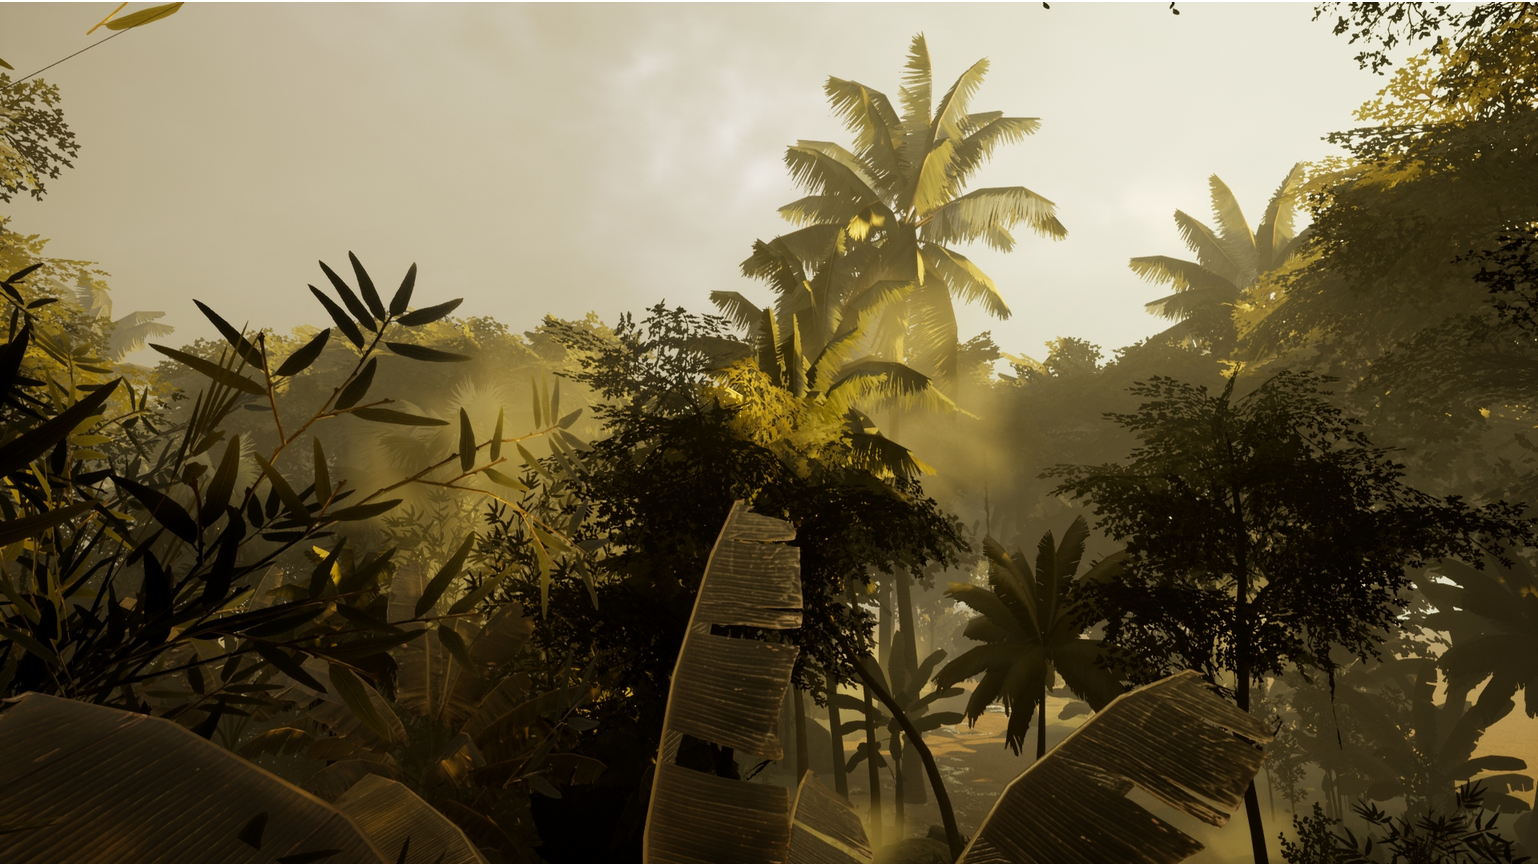
\includegraphics[width = 0.9\linewidth]{figs/UE4JungleProto.png}
%     \caption{Unreal Engine 4 Jungle Environment}
%     \label{fig:UE4JungleProto}
% \end{figure}
%\subsection{Security}



% \begin{figure}[h]
%     \centering
%     \includegraphics[width = 3 in]{figs/GazArena.png}
%     \caption{Gazebo Environment}
%     \label{fig:GazArena}
% \end{figure}

%andia National Labs considers examples where there is a compound that has a sensitive area that must be protected and is surrounded by land that contains wild life. Sometimes when an intruder is detected, the security system cannot determine if the threat is real or if there is simply an animal wandering around. A security officer must then go out and find the intruder to determine the state of the threat. In order to reduce wasted time, actively tracking that threat to provide the security personnel with a small region to search instead of a last known location saves resources. 

%and of security around a sensitive compound where tracking potential intruders is required for security personnel to make contact with and determine if the threat is real or false.




\subsection{Robot Platforms}

We use two robot simulation platforms to demonstrate the generality and applicability of the platform-agnostic methodology developed in this paper:
\begin{enumerate}
    \item An Iris quadcopter, which uses the PX4 flight stack and is capable of waypoint control.
    \item Stanley Innovations segway, which uses the ROS navigation stack for mapping, waypoint control, and autonomous obstacle avoidance. 
\end{enumerate}
To simulate the sensor output, we directly access the ground truth position of the moving target and add noise. We model the sensor and state estimation uncertainty as described in section \ref{sec:sensefunction} using a simulated 360 degree LiDAR with range of  $10$ meters, angular resolution of 1 degree, range accuracy of $\pm 3$ cm.


The function $vis$ is built directly from the sensor range parameter. To construct the function $sense$ we use a worst-case conservative Gaussian noise model. Given a sensor measurement, let $0 \leq p(l) \leq 1$ be the probability the target is in location $l$. We construct the uncertainty set $U$ of possible target states for each sensor measurement $sense(l_a,l_t)$ by including all states with a probability greater than $\delta$ where $0\leq \delta \leq 1$ can be set by the user. In the following simulations, we use $\delta = 0.95$. Informally, if a target is in sensor range, the agent's belief consists of \emph{all states} at which the target is with a probability greater than or equal to $5\%$. We note that, since the function $obs$ depends only on the sensors, the function needs to be constructed only once and can be used for all robots that use the same sensors. 
We test the synthesized surveillance strategies synthesized in two environments. One is an open urban-like setting modelled in Unreal Engine 4 depicted in Figure \ref{fig:UE4city}. A quadcopter acts as the surveilling agent and another acts as a potential intruder. In the second scenario, we consider an enclosed compound-like environment modelled in Gazebo as shown in Figure \ref{fig:GazArena}. The Iris quadcopter is tasked with tracking a hostile target (the Stanley Innovations segway) and maintaining sufficient knowledge of its location. We allow a human to directly control the rover and demonstrate the corresponding real-time response of the quadcopter to satisfy its surveillance task. We also perform the same experiment with the quadcopter controlled by a human and the Segway as the autonomous surveilling agent to emphasise that the framework is agnostic to the specific underlying hardware and can be easily applied. 
  
We contrast the surveillance needs and the qualitatively different resulting behaviours of the synthesized strategies for the agents in these two environments.

\begin{figure}
\centering


\subfloat[Urban environment modeled in Unreal Engine 4 \label{fig:UE4city}]{
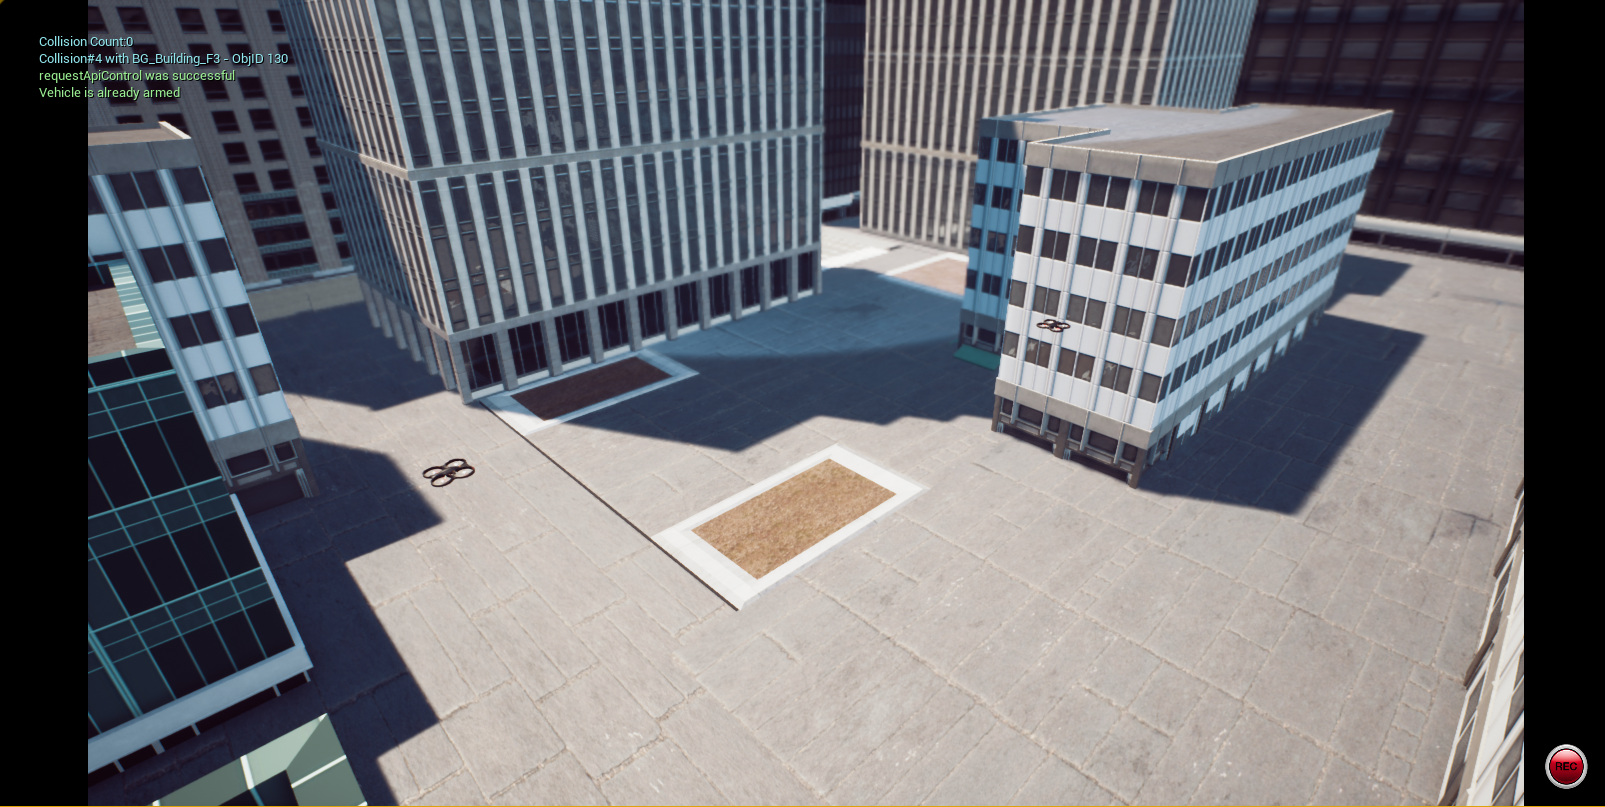
\includegraphics[width = 0.9\linewidth]{Surveillance/figs/unreal_city.png}}

\subfloat[Enclosed compound modelled in Gazebo \label{fig:GazArena}]{
\includegraphics[width = 0.9\linewidth]{Surveillance/figs/GazArena.png}}

\subfloat[Iris quadcopter used for autonomous surveillance \label{fig:sandiauav}]{
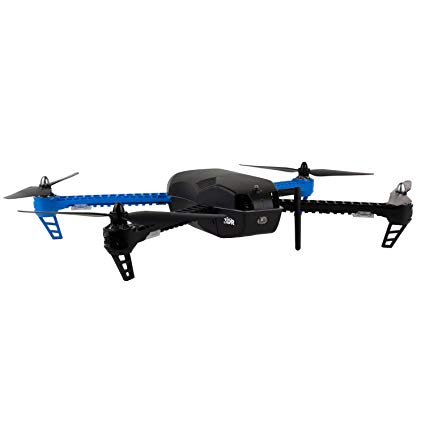
\includegraphics[width = 0.43\linewidth]{Surveillance/figs/quad.jpg}
} \hspace{0.05\linewidth}
\subfloat[Stanley innovations segway vehicle acting as a hostile target \label{fig:stanleyrobot}]{
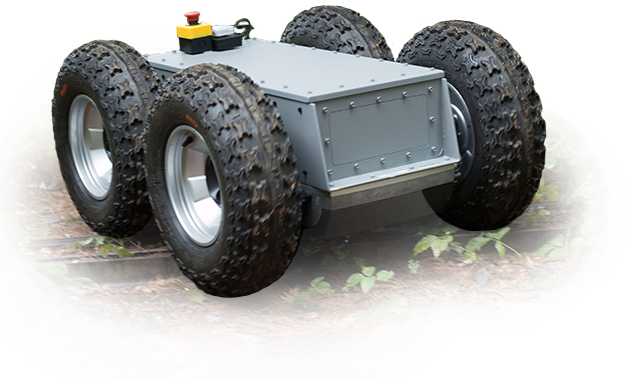
\includegraphics[width = 0.43\linewidth]{Surveillance/figs/Rugged-All-Terrain.png}
}

\caption{Case study for a security application. The vehicles are simulated in either Gazebo environment shown in \ref{fig:GazArena} or a UE4 environment shown in \ref{fig:GazArena}. A user can act as an `intruder' by controlling a target \ref{fig:stanleyrobot}. The UAV in \ref{fig:sandiauav} must autonomously react to guarantee the surveillance mission is satisfied. }
\label{fig:SandiaCaseSTudy}
\end{figure}

%%%%%%%%%%%%%%%%%%%%%%%%%%%%%%%%%%%%%%%%%%%%%%%%%%%%%%%%%%%%%%%%%%%%%%%%%%%%%%%%

\section{GAMES WITH SURVEILLANCE OBJECTIVES}\label{sec:gamedef}
%\subsection{Overview}\label{sec:problemoverview}
 Consider an environment consisting of an operating space and a network formed from a series of $k$ UAM vertiport hubs labeled $V_1,\cdots,V_k$. A UAM vertiport hub (henceforth referred to as a vertihub) consists of a grouping of multiple vertiports, each of which may have multiple takeoff/landing pads. A vertihub is responsible for managing requests by UAM vehicles (henceforth referred to as vehicles) to either \emph{land at} or \emph{take off from} a desired vertiport in its region or \emph{pass through} to a neighboring region. Each vertiport inside a vertihub is in charge of taking off and landing vehicles at its landing pads. An example of such an environment is illustrated in Figure~\ref{fig:RegionsOutline}. Note that vertihub control regions need not be circular. 
\begin{example}
The vertihub controller for region $V_6$ in Figure~\ref{fig:RegionsOutline} controls the operational area defined by $V_6 - (V_6 \cap V_5)$. The area of overlap $H_{56} = V_5 \cap V_6$ is the region where the handoff takes place, wherein the vertihub controller of the region the vehicle is about to enter takes responsibility for the vehicle.
Hence, $V_6$ can force vehicles incoming from $V_5$ to loiter in the handoff region $H_{56}$ until it is safe to allow them to enter.
\end{example}

The number of vehicles allowed inside each vertihub is upper bounded both by the separation standards between the vehicles as well as with the complexity of the airspace (e.g., intersection with general aviation traffic etc.).
Vertihubs cannot accept vehicles (i.e., accept a handoff) if the additional vehicle exceeds the maximum operational capacity or induces a conflict. Furthermore, vertiports cannot allow vehicles to take-off if it will violate the maximum operational capacity of the vertihub, and must force incoming vehicles to loiter if all of their pads are occupied. In order to avoid violating airspace requirements and to avoid build up of loitering vehicles (which can delay vehicles desiring to pass through or create safety issues), a vertiport must coordinate with its corresponding vertihub. We model the vertihub controller and vertiport controllers as \emph{reactive systems}.
%The hub can then act tactically by blocking a vehicle's entry to the region by making it loiter in a \emph{handoff region}.

\paragraph*{\textbf{Definition}}
We consider a finite set $\inp$ ($\out$) of Boolean \emph{inputs (outputs)}.
The input alphabet is
$\ialphabet=2^\inp$, the output alphabet is $\oalphabet=2^O$, and
$\alphabet=\ialphabet \times \oalphabet$. The set of finite (infinite) traces
over $\alphabet$ is denoted by $\alphabet^*$ ($\alphabet^\omega$), and
we define $\alphabet^{\infty} = \alphabet^* \cup \alphabet^\omega$.  A reactive system is a
tuple $\design = (\states,q_{0},\ialphabet,\oalphabet,\delta,\lambda)$,
where
$\states$ is a finite set of states,
$q_{0} \in \states$ is the initial state,
$\ialphabet$ is the input alphabet,
$\oalphabet$ is the output alphabet,
$\delta: \states \times \Sigma_{\inp} \to \states$ is the complete transition function, and $\lambda : \states \times \Sigma_{\inp} \to \Sigma_{\out}$ is the output function.
%
Given an input trace $\itrace = x_0 x_1 \ldots \in \ialphabet^\infty$, a reactive system $\mathcal{\design}$ produces an
output trace $\otrace = \mathcal{\design}(\itrace) = \lambda(q_0, x_0)
\lambda(q_1, x_1) \ldots \in \oalphabet^\infty$ with $q_{i+1} = \delta(q_i, x_i)$ for all $i \ge 0$.
The set of words produced by
$\mathcal{\design}$ is denoted $\lang(\mathcal{\design}) = \{\itrace \parallel \otrace \in
\alphabet^\infty \mid \mathcal{\design}(\itrace) = \otrace\}$.



\begin{figure}[h!]
	\centering

\newcommand{\OperatorSpace}[5]{
				%\draw[rounded corners = 15pt,dashed] (#1-#4,#2-#5) rectangle (#1+#4,#2+#5);
		\fill[fill=green,opacity=0.2] (#1,#2) circle (#3);
		\draw[draw = black,dashed](#1,#2) circle (#3);
		%\node at (#1,#2-#5+0.5) {$V_{#6}$};
	}

	

		\subfloat[ Example UAM operating environment \label{fig:RegionsOutline}]{
		\scalebox{1.75}{
		\begin{tikzpicture}[scale=0.3]
			\OperatorSpace{0}{0}{3}{5}{5}
			%\node at (-4.25,4.25){$S_1$};
			\node at (-1.5,1.5){$V_1$};
			\OperatorSpace{3}{-4}{3}{5}{5}
			%\node at (-1.25,-8.25){$S_2$};
			\node at (2.5,-4.5){$V_2$};
			\node[red] at (2.5,3) (H13) {$H_{13}$};
			\draw [->,red,line width = 0.75mm] (H13) -- (2.5,1.25);
			\OperatorSpace{5}{0}{3}{5}{6}
			%\node at (5-4.25,5.5){$S_3$};
			\node at (5-0.5,2){$V_3$};
			\node[red] at (6.5,3.5) (H35) {$H_{35}$};
			\draw [->,red,line width = 0.75mm] (H35) -- (6.75,0.65);
			\OperatorSpace{10}{0}{4}{6}{7}
			
			\node at (8.5-0.5,-5.5){$V_4$};
% 			\node[red] at (6.5,3.5) (H35) {$H_{35}$};
			\draw [->,red,line width = 0.75mm] (H35) -- (6.75,0.65);
			\OperatorSpace{6.5}{-4}{2.5}{0}{0}
			
			%\node at (10+5.25,-6.5){$S_5$};
			\node at (10+1.5,-1.5){$V_5$};
			\OperatorSpace{15}{2}{3}{5}{5}
			\fill[blue] (-1.5,-1.5) rectangle (-1,-1);
			%\node at (15-4.25,5+3.25){$S_6$};
			\node at (15,3.5){$V_6$};
			\node[red] at (11,4.5) (H56) {$H_{56}$};
			\draw [->,red,line width = 0.75mm] (H56) -- (12.5,2.75);
			\draw (17,3) node[cross,blue]{};
			\draw[blue,line width = 0.5mm] plot [smooth,tension=1] coordinates{(-1.5,-1.5) (3,0.5) (10,0) (17,3)};
			\draw (-0.5,2) node[cross,black]{};
			\fill[black] (7.5,-5.5) rectangle (7.0,-5.0);
			\draw[black,line width = 0.5mm] plot [smooth,tension=1] coordinates{(-0.5,2) (3,-0.5) (7,-5.0)};
			
		\end{tikzpicture}}}\\
\subfloat[Connectivity graph \label{fig:Environment_directed}]{
\scalebox{1.25}{
\begin{tikzpicture}[auto,node distance=8mm,>=latex,font=\small]
        \tikzstyle{round} = [thick,draw=black,circle]
\tikzstyle{action} = [circle, draw, fill=black,inner sep=0pt, minimum size=4pt]
\node[round] (s1) {$\design_{1}$};
\node[round, right=15mm of s1] (s3){$\design_{3}$};
\node[round, below right=15mm and 5mm of s1] (s2){$\design_{2}$};
\node[round, right=15mm of s3] (s5){$\design_{5}$};
\node[round, right=10mm of s2] (s4){$\design_{4}$};
\node[round, right= 10mm of s5] (s6){$\design_{6}$};

\draw[<->] (s1) -- node[left]{$e_{12}$} (s2);
\path[<->,draw] (s1) -- node{$e_{13}$} (s3);
\path[<->,draw] (s2) -- node{$e_{23}$} (s3);
\path[<->,draw] (s2) -- node{$e_{24}$} (s4);
\path[<->,draw] (s3) -- node{$e_{34}$} (s4);
\path[<->,draw] (s3) -- node{$e_{35}$} (s5);
\path[<->,draw] (s4) -- node[right]{$e_{45}$} (s5);
\path[<->,draw] (s5) -- node[below]{$e_{56}$} (s6);

% \path[->,draw] (s1) edge[loop above] node {$e_{1}$} (s1);
% \path[->,draw] (s2) edge[loop below] node {$e_{2}$} (s2);
% \path[->,draw] (s3) edge[loop above] node {$e_{3}$} (s3);
% \path[->,draw] (s4) edge[loop below] node {$e_{4}$} (s4);
% \path[->,draw] (s5) edge[loop above] node {$e_{5}$} (s5);
% \path[->,draw] (s6) edge[loop above] node {$e_{6}$} (s6);

\end{tikzpicture}}}

\caption{
(a) Green circles correspond to the region of a vertihub. UAM vehicles (blue and black) move between origin-destination vertiports in the environment.
(b)
The corresponding connectivity graph $G_\design$ of the vertihub controllers $\design$ modeling the sectors $V$. 
Each edge $e_{ij}$ corresponds to $\design_i$ and  $\design_j$ being connected, i.e., the outputs of $\design_i$ are inputs to $\design_j$ and vice versa.
}
%		\setlength{\belowcaptionskip}{-2pt}
	       %\label{fig:RegionsOutline}
    \end{figure}

Ensuring the safety of the takeoff and landing operations at vertiports that share the same airspace must be balanced with bounding the delays experienced by vehicles. Furthermore, vehicles cannot loiter indefinitely due to energy constraints.
Hence, vertihubs must additionally guarantee a finite upper bound on the delays experienced by vehicles.
All of these requirement guarantees (and others) can be expressed as \emph{temporal logic specifications} that controllers must satisfy. %In addition to satisfying their own specification, each controller must not cause other controllers to violate their specification. We formalize this notion in Section~\ref{sec:distshield}. 


\paragraph*{\textbf{Definition}}
%
A \emph{linear temporal logic (LTL) specification} $\varphi$ defines a set of allowed traces $L(\varphi) \subseteq \plays(\design)$ for the reactive system $\design$.  A reactive system $\design$ is \emph{winning} with respect to specification $\varphi$ iff $L(\design) \subseteq L(\varphi)$ and is denoted $\design \models \varphi$. Given a set of propositions \texttt{AP}, a formula in LTL describes a language in $(2^{\texttt{AP}})^\omega$. LTL extends Boolean logic by the introduction of temporal operators such as $\bigcirc$ (next time), $\LTLglobally$ (always), $\LTLfinally$ (eventually), and $\mathcal{U}$ (until). 


 Informally, the main problem addressed in this paper is designing \emph{controllers} for vertihubs and vertiports that guarantee all safety and progress requirements, assuming they have been correctly captured in the design process. More formally, the task of computing a satisfying controller in reactive systems involves constructing the function $\lambda$ and can be typically framed as computing the \emph{winning strategy of a game}. 



\paragraph*{\textbf{Definition}}
%
A \emph{game structure} is a tuple 
$\game = (\states, \state_0, \alphabet, \delta,\Acc)$,
where 
\begin{itemize}
\item $\states$ is a finite set of states, $\state_0 \in \states$ the initial state,
\item $\alphabet = (\ialphabet \times \oalphabet)$ is the alphabet of actions available to the environment and the controller respectively, 
\item $\delta: \states \times \alphabet \rightarrow \states$
is a complete transition function, that maps each state, input (environment action) and output (controller action) to a successor state.
\item $\Acc: \left(\states \times \alphabet \times \states\right)^\omega \rightarrow \mathbb{B}$ is the \emph{winning condition} of the game. 
% \item $\mathcal L:\gstates
% \rightarrow \ialphabet \times \oalphabet$ is the labeling
% function.
\end{itemize}


At every state $\state \in \states$ (starting with
$\state_0$), the environment chooses an input $\isymb \in
\ialphabet$, and then the controller chooses some output $\osymb
\in \oalphabet$. These choices define the next state $\state' =
\delta(\state,(\isymb, \osymb))$, and the process then continues from $\state'$. This order of moves
ensures that at each step the controller's action reacts to the \emph{current}
action of the environment. The resulting
(infinite) sequence $\pi = (\state_0,\symb_{\inp,0},
\symb_{\out,0}, \state_1) (\state_1,\symb_{\inp,1},
\symb_{\out,1}, \state_2) \ldots$ is
called a \emph{play}, where $\state_0$ is the initial state, and for every $i \geq 0$ we have that $\state_{i+1} = \delta(\state_i,\symb_{\inp,i},\symb_{\out,i})$.  A play $\pi$ is \emph{winning} if $\Acc(\pi) = \top$. 
%The set $L(\game)$ is the set of all plays in the game $\game$.


We consider winning conditions expressed from a fragment of LTL specifications called \emph{Generalized Reactivity 1} (GR(1)), which is common in a variety of practical applications~\cite{Moarref18,Alonso18,bh18,Maoz2015}.
A GR(1) winning condition is defined by sets of states $S_\inp, S_\out \subseteq \states$, $E_i \subseteq \states$ for $i=1,\ldots,m$ and $F_j \subseteq \states$ for $j=1,\ldots,n$, and consists of all plays $ \pi$ such that if $\pi \in \LTLglobally S_\inp \cap \LTLglobally\,\LTLfinally\, E_{i}$ for all $i=1,\ldots,m$, then $\pi \in \LTLglobally S_\out \cap \LTLglobally\,\LTLfinally\, F_{j}$ for all $j=1,\ldots,n$. Intuitively, for a play $ \pi$ to be winning, whenever the environment satisfies the assumptions $\LTLglobally\, S_\inp,\LTLglobally\,\LTLfinally\, E_{1},\ldots,\LTLglobally\,\LTLfinally\, E_{m}$, then the controller must satisfy all the guarantees $\LTLglobally\, S_\out,\LTLglobally\,\LTLfinally\, F_{j},\ldots,\LTLglobally\,\LTLfinally\, F_{n}$. By abuse of logical operators, we abbreviate GR(1)  conditions as
$$\left(\LTLglobally\, S_\inp \wedge \bigwedge_{i=1}^{m}  \LTLglobally\,\LTLfinally\, E_{i}\right) \implies
\left(\LTLglobally\, S_\out \wedge \bigwedge_{j=1}^{n} \LTLglobally\,\LTLfinally\,F_{j}\right).$$


\paragraph*{\textbf{Definition}}
%
% We seek to compute a strategy for the agent to enforce a given winning condition, or determine that it cannot ensure winning.

A \emph{strategy for the controller} is a function $\rho_\out:
\prefs(\game) \times \ialphabet \rightarrow
\oalphabet$ which maps a prefix of a run (the history of the play so far) and an action of the environment to an action of the controller. 
A \emph{strategy for the environment} is a function $\rho_\inp: \prefs(\game)\rightarrow \ialphabet$ that maps the prefix of the play so far to an action of the environment. We denote the sets of all strategies for the controller and for the environment by $\mathcal{M}_\out $ and $\mathcal{M}_\inp$ respectively.

Every pair of strategies $\rho_\out \in \mathcal{M}_\out$ for the controller and $\rho_\inp \in \mathcal{M}_\inp$ for the environment define a play, denoted by $\Pi(\rho_\out,\rho_\inp)$. More precisely,  
$\Pi(\rho_\out,\rho_\inp) = \pi = (\state_0,\symb_{\inp,0},\symb_{\out,0}, \state_1) 
(\state_1,\symb_{\inp,1}, \symb_{\out,1}, \state_2) \ldots \in \plays(\game)$
where
for every $i \geq 0$, $\symb_{\inp,i} = \rho_\inp(\pi[0,i])$ and $\symb_{\out,i} = \rho_\out(\pi[0,i],\symb_{\inp,i})$.
Similarly, we define the set of plays starting at a state $g$ that are consistent with $\rho_\out$, denoted $\plays(\design,\rho_\out,g)$.

Given a game structure $\design$ and a winning condition $\varphi$ for the agent, the synthesis problem is to generate a strategy $\rho_\out\in \mathcal{M}_\out$ for the controller such that for every strategy $\rho_\inp \in \mathcal{M}_\inp$ for the environment it holds that $\Pi(\rho_\inp,\rho_\out) \in \varphi$, i.e., all resulting plays satisfy $\varphi$.
In such cases we say that \emph{$\rho_\out$ satisfies $\spec$}, denoted $\rho_\out\models\spec$.




% \subsection{Basic notations}
% We consider reactive systems with a finite set $\inp$ ($\out$) of Boolean \emph{inputs (outputs)}.
% The input alphabet is
% $\ialphabet=2^\inp$, the output alphabet is $\oalphabet=2^O$, and
% $\alphabet=\ialphabet \times \oalphabet$. The set of finite (infinite) traces
% over $\alphabet$ is denoted by $\alphabet^*$ ($\alphabet^\omega$), and
% we define $\alphabet^{\infty} = \alphabet^* \cup \alphabet^\omega$.  

% \subsection{Reactive systems}

% A \emph{reactive system} is defined by a
% tuple $\design = (\states,q_{0},\ialphabet,\oalphabet,\delta,\lambda)$,
% where
% $\states$ is a finite set of states,
% $q_{0} \in \states$ is the initial state,
% $\ialphabet$ is the input alphabet,
% $\oalphabet$ is the output alphabet,
% $\delta: \states \times \Sigma_{\inp} \to \states$ is the complete transition function, and $\lambda : \states \times \Sigma_{\inp} \to \Sigma_{\out}$ is the output function.
% %
% Given an input trace $\itrace = x_0 x_1 \ldots \in \ialphabet^\infty$, a reactive system $\mathcal{\design}$ produces an
% output trace $\otrace = \mathcal{\design}(\itrace) = \lambda(q_0, x_0)
% \lambda(q_1, x_1) \ldots \in \oalphabet^\infty$ with $q_{i+1} = \delta(q_i, x_i)$ for all $i \ge 0$.
% The set of words produced by
% $\mathcal{\design}$ is denoted $\lang(\mathcal{\design}) = \{\itrace \parallel \otrace \in
% \alphabet^\infty \mid \mathcal{\design}(\itrace) = \otrace\}$.
% In reactive systems, the synthesis task involves constructing the function $\lambda$ and can be typically framed as computing the \emph{winning strategy of a game}. 




% \subsection{Specifications}
% %
% A \emph{linear temporal logic (LTL) specification} $\varphi$ defines a set of allowed traces $L(\varphi) \subseteq \plays(\design)$ for the reactive system $\design$.  A reactive system $\design$ is \emph{winning} with respect to specification $\varphi$ iff $L(\design) \subseteq L(\varphi)$ and is denoted $\design \models \varphi$. Given a set of propositions \texttt{AP}, a formula in linear temporal logic (LTL) describes a language in $(2^{\texttt{AP}})^\omega$. LTL extends Boolean logic by the introduction of temporal operators such as $\bigcirc$ (next time), $\LTLglobally$ (always), $\LTLfinally$ (eventually), and $\mathcal{U}$ (until). 





%In the following, we make use of LTL operators $\LTLglobally$ and $\LTLfinally$ which are operators for \emph{always} and \emph{eventually} respectively. For full details on LTL syntax, we refer the reader to~\cite{MCBook}.

% A \emph{safety} winning condition $\varphi$ is defined by a set of states $S \subseteq G$ and is such that for a play $\overline{\pi}\in \plays(\game)$ we have $\overline\pi\in\varphi$ if and only if $g_i \in S$ for all $i \in\mathbb{N}$.

% A \emph{\buchi} winning condition $\varphi$ is defined by a set of states $F \subseteq G$ and is such that for a play $\overline{\pi} \in \plays(\game)$ we have $\overline\pi\in\varphi$ iff $\inf(\overline{\pi})\cap F \neq \emptyset$,  where $\inf(\overline{\pi}) \subseteq G$ is the set of states that occur infinitely often in $\overline{\pi}$.
% We abbreviate the \buchi condition as $\varphi = \LTLglobally\,\LTLfinally\, F$.



%Note that if the agent has a winning condition $\varphi$, then all plays in $\plays(\game)\setminus\varphi$ are winning for the environment player.




\iffalse
\subsection{Serial composition}
Consider two reactive systems  $\design = (\states,q_{0},\ialphabet,\oalphabet,\delta,\lambda)$ and $\shield = (\states', q_{0}',\alphabet', \delta',\lambda')$.
The \emph{serial composition} of $\design$ and $\shield$ is obtained by feeding the output of $\design$ to $\shield$ and results in a new reactive system $\design \comp \shield=(\hat{\states}, \hat{q_{0}}, \ialphabet,\oalphabet, \hat{\delta},
\hat{\lambda})$, where
   $\hat{\states} = \states \times \states'$,
   $\hat{q_{0}} = (q_{0}, q_{0}')$,
   $\hat{\delta}((q,q'),\isymb) = (\delta(q,\isymb), \delta'(q',(\isymb,\lambda(q,\isymb))))$, and
   $\hat{\lambda}((q,q'),\isymb) = \lambda'(q',(\isymb,\lambda(q, \isymb)))$.
\fi
   
% \subsubsection{Multi-agent reactive systems}
% A \emph{multi-agent reactive system} $\design$ is a tuple $(\proc, \ialphabet,  \oalphabet)$, where $\proc = \{\proc_1,\ldots,\proc_n\}$ is a set of agents, where each $\proc_i = (\states_i, q_{0,i},\ialphabeti,\oalphabeti,\delta_i,\lambda_i)$ is a reactive system. For more details on the construction of multi-agent reactive system, we refer the reader to \cite{multiagentshield}. 

%Since we perform a localized synthesis procedure in this paper, the multi-agent reactive systems dealt with in \cite{multiagentshield} will instead be decentralized single-agent reactive systems.
%
% While multiple agents may be able to read the same input variables to indicate
% broadcast from the environment, the sets of outputs are pairwise disjoint: for $i \neq j$, we have $\out_i \cap \out_j = \emptyset$. Furthermore, agents cannot directly read each others outputs, that is, for all $i$ and $j$, we have $\out_i \cap \inp_j = \emptyset$. The outputs of the multiagent system  $\design$ are $\out = \bigcup_{i=1}^n \out_i$, and its inputs are $\inp  = \bigcup_{i=1}^n \inp_i$.
% %
% The joint behaviour of the multi-agent system is a reactive system 
% $\design=(\states, q_{0}, \ialphabet,\oalphabet, \delta,
% \lambda)$ defined as follows: the set $\states = \bigotimes_i \states_i$ of states is formed by the product of
% the states of all agents $\proc_i \in \proc$. The initial state $q_{0}$ is formed
% by the initial states $q_{0,i}$ of all $\proc_i \in \proc$. The transition function $\delta$ updates, for each agent $\proc_i \in \proc$, the $\states_i$ part of the state in accordance with the transition function $\delta_i$, using
% the projection $\symb(I_p)$ as input. The output function $\lambda$ labels each state with the
% union of the outputs of all $\proc_i \in \proc$ according to $\lambda_i$.



% \subsection{Specifications}

% A \emph{specification} $\spec$ defines a set $\lang(\spec) \subseteq \alphabet^\infty$ of allowed traces.
% %
% A reactive system $\design$ \emph{realizes} $\spec$, denoted by $\design \models \spec$, iff
% $\lang(\design) \subseteq \lang(\spec)$.
% Given a set of propositions $\mathsf{AP}$, a formula in \emph{linear temporal logic} (LTL) describes a language in $(2^\mathsf{AP})^\omega$. LTL extends Boolean logic by the introduction of temporal operators such as $\LTLX$ (next time), $\LTLG$ (globally), $\LTLF$ (eventually), and $\LTLU$ (until)~\cite{Pnueli77}.
% %
% $\varphi$ is called a \emph{safety specification} if every trace $\trace$ that is not in  $\lang(\spec)$  has a prefix $\tau$ such that all words starting with $\tau$ are also not in the language $\lang(\spec)$.
% We represent a safety specification $\varphi$ by a safety automaton
% $\varphi = (Q, q_0, \alphabet, \delta, F)$, where $F\subseteq Q$ is a set of safe states.

% \subsection{Games}
% %
% A game is a tuple $\game = (\gstates,
% \ginit, \alphabet, \delta, \Acc, \Val)$,
% where $\gstates$ is a finite set of states, $\ginit \in \gstates$ is the initial state,
% $\delta: \gstates \times \alphabet \rightarrow \gstates$
% is a complete transition function, $\Acc: (\gstates \times \alphabet \times \gstates)^\omega \rightarrow \bools$ is a winning condition
% and defines the qualitative objective of the game, and $\Val: (\gstates \times \alphabet \times \gstates)^\omega \rightarrow \mathbb{R} \cup \{-\infty, \infty \}$ is a value function defining the quantitative objective of the game. A game can have a winning condition, a value function, or both.
% %
% The game is played  by two players:  the system and the environment. In every state $g\in \gstates$
% (starting with $\ginit$), the environment chooses an input
% $\isymb \in \ialphabet$, and then the system chooses some output $\osymb \in \oalphabet$. These choices define the next state $g' = \delta(g,(\isymb, \osymb))$, and so on. The resulting (infinite)
% sequence $\overline{\pi} = (g_0,\isymb, \osymb, g_1) (g_1,\isymb, \osymb, g_2) \ldots$ is called a \emph{play}.
% A deterministic  \emph{strategy} for the environment is a function
% $\rho_e: \gstates^* \rightarrow \ialphabet$.
% A nondeterministic \emph{strategy} for the system is a relation $\rho_s:
% \gstates^* \times \ialphabet \rightarrow 2^{\oalphabet}$ and a
% deterministic  strategy for the system is a function $\rho_s:
% \gstates^* \times \ialphabet \rightarrow \oalphabet$.\looseness=-1

% A play $\overline{\pi}$ is \emph{won} by the system iff $\Acc(\overline{\pi})=\top$.
%  A strategy is \emph{winning} for the system if all plays $\overline{\pi}$ that can be
% constructed when defining the outputs using the strategy result in
% $\Acc(\overline{\pi})=\top$. The \emph{winning region} $\Win$ is the set of states
% from which a winning strategy exists.
% A \emph{permissive} winning strategy  $\rho_s:
% \gstates^* \times \ialphabet \rightarrow 2^{\oalphabet}$ is a strategy that is not only winning for the system, but also contains all deterministic winning strategies.

% A \emph{safety game} defines $\Acc$ via a set $F\subseteq \gstates$ of
% safe states: $\Acc(\overline{\pi})=\top$ iff $g_i \in F$ for all $i \geq 0$, i.e., if only safe states are visited in the play $\overline{\pi}$. Otherwise, $\Acc(\overline{\pi})=\bot$. The quantitative objective of the system is to minimize $\Val(\overline{\pi})$, while the environment
%  tries to maximize it.\looseness=-1
%If a safety game is won by the system player, then there exists a permissive strategy $\rho_s$ that is \emph{memoryless}, i.e., has the form $\rho_s:
%\gstates \times \ialphabet \rightarrow 2^{\oalphabet}$.
%
% The \emph{\buchi} winning condition is $\Acc(\overline{\pi})=\top$ iff $\inf(\overline{\pi})
% \cap F \neq \emptyset$, where $F \subseteq Q$ is
% the set of accepting states and $\inf(\overline{\pi})$ is the set of states that occur infinitely often in $\overline{\pi}$.
% We abbreviate the \buchi condition as $\mathcal{B}(F)$.
% A \emph{Generalized Reactivity 1} (GR(1))
% acceptance condition is a predicate $\bigwedge_{i=1}^{m} \mathcal{B}(E_{i}) \rightarrow \bigwedge_{i=1}^{n} \mathcal{B}(F_{i})$, with
% $E_i \subseteq Q$ and $F_i \subseteq Q$.
%  A \emph{Streett}
% acceptance condition 
% %with $k$ pairs 
% is 
%  $\bigwedge_{i=1}^{k} \mathcal{B}(E_{i}) \rightarrow \mathcal{B}(F_{i})$.


%
\iffalse MEAN-PAYOFF
A \emph{mean-payoff game} is a game where $\Val$ is defined via an edge labeling function $r :
\delta \rightarrow \{-W,\dots, W\}$, which assigns values between $-W$ and $W$ to edges. For a play $\pi =
e_0 e_1 e_2 \dots \in \delta^\omega, \Val(\overline{\pi}) = \lim \sup_{n\rightarrow\infty} \frac{1}{n+1} \sum_{i=0}^{n} r(e_i)$.
\fi


% \subsubsection{Properties of traces}
% A finite trace $\trace
% \in \alphabet^*$ is \emph{wrong} w.r.t. a specification $\varphi$, if the corresponding play cannot be won,
% i.e., if there is no way for the system to guarantee that any
% extension of $\trace$ satisfies $\spec$.
% An output $\osymb$
% is called \emph{wrong} for a trace $\trace$ and input $\isymb$, if it makes the trace wrong, i.e. when $\trace$ is not wrong, but $\trace \cdot (\isymb,\osymb)$ is. Given a sequence $(\itrace\parallel\otrace\parallel\otrace') \in (\ialphabet\times\oalphabet\times\oalphabet)^\infty$, we denote with $\widx(\itrace\parallel\otrace\parallel\otrace')$ the positions of occurrences of wrong outputs in $\otrace$. Formally, $i \in \widx(\itrace\parallel\otrace\parallel\otrace')$ iff  $\otrace[i]$ is wrong for the trace
% $(\itrace[0,i)\parallel\otrace'[0,i))$ and the input $\itrace[i]$.

% %
% We denote with $\Proc = \{1,\ldots,n\}$ the set of agent ids of a multi-agent system $\design$.
% %
% For a set $\Pi \subseteq \Proc$, we define $O_{\Pi} = \bigcup_{p \in \Pi} O_p$ and $\alphabet_{O_{\Pi}} = 2^{O_{\Pi}}$. For $\osymb \in \oalphabet$ and $p \in \Proc$, we denote with $\osymb(O_p)$ the projection of $\osymb$ on $O_p$. For $\Pi \subseteq \Proc$, we define $\osymb(O_{\Pi})$ similarly. 

% For  $\osymb,  \osymb' \in \oalphabet$, the set $\Diff(\osymb,\osymb') = \{p \in \Proc \mid \osymb(O_p) \neq \osymb'(O_p)\}$ gives the set of agents whose outputs in $\osymb$ differ from those in $\osymb'$.
% Let $(\otrace \parallel \otrace')\in (\oalphabet\times\oalphabet)^\infty$ be a sequence of output pairs.
% We call $(\otrace \parallel\otrace')$ a \emph{deviation period} if (1) $\otrace[i] \neq \otrace'[i ]$ for every $i < |\otrace|$  and (2) if $|\otrace| < \infty$, then $\otrace[|\otrace|] = \otrace'[|\otrace|]$.
% Thus, a deviation period is either a finite sequence $(\otrace\parallel\otrace')$  consisting of differing outputs followed by a last letter where the two outputs agree, or an infinite sequence $(\otrace\parallel\otrace')$ where the outputs always differ. \looseness=-1
%We denote with $\Deviations(\otrace||\otrace')$ the set of all deviation periods of $(\otrace||\otrace')$.




%
%%%%%%%%%%%%%%%%%%%%%%%%%%%%%%%%%%%%%%%%%%%%%%%%%%%%%%%%%%%%%%%%%%%%%%%%%%%%%%%%%
%
\section{BELIEF-SET ABSTRACTION}
%\subsection{Abstract Belief-Set Games}
%We used the belief-set game structure in order to state the surveillance objective of the agent. While in principle it is possible to solve the surveillance strategy synthesis problem on this game, this is in most cases computationally infeasible, since the size of this game is exponential in the size of the original game. To circumvent this construction we propose an abstraction-based method, that given a surveillance game structure and a partition of the set of the target's locations, yields an approximation that is sound with respect to surveillance objectives for the agent.

We will use a combination of two ways to approximate belief states. First, note that we can overapproximate the agent's current belief by considering the set of possible locations of the target returned by the sensors at that step, thus, essentially, losing some of the information about which of the locations in the returned set are actually reachable at that step. While these sets often provide a useful approximation, an abstraction based solely on the observations will in general not be able to precisely capture the agent's belief when necessary. To this end, we include a different type of approximation which allows for arbitrary precision. It is based on partitioning the set of locations into finitely many sets of locations, and using a combination of such sets to overapproximate the agent's belief. In the extreme case when each of these sets consists of a single location the abstraction is capable of precisely expressing every possible belief set. In practice, however, it is often the case that coarser partitions are sufficient for finding a winning strategy for the agent when one exists.

We begin by defining abstraction partitions and the associated abstraction and concretization functions, and then use them to define the abstract game associated with them.

\bigskip
An \emph{abstraction partition} is a family $\partition = \{Q_i\}_{i=1}^n$ of subsets of $L$, $Q_i \subseteq L$ such that the following hold:
\begin{itemize}
\item $\bigcup_{i=1}^n Q_i = L$ and $Q_i \cap Q_j = \emptyset$ for all $i \neq j$;
\item For each $p \in \AP$, $Q \in \partition$ and $l_a \in L$, it holds that $(l_a,l_t') \models p$ iff $(l_a,l_t'') \models p$ for every $l_t',l_t'' \in Q$.
\end{itemize}
Intuitively, these conditions mean that $\mathcal Q$ partitions the set of locations of the target, and the concrete locations in each of the sets in $\partition$ agree on the value of the  propositions in $\AP$.

If $\partition' =  \{Q_i'\}_{i=1}^m$ is a family of subsets of $L$ such that $\bigcup_{i=1}^m Q_i' = L$ and for each $Q_i' \in \partition'$ there exists $Q_j \in \partition$ such that $Q_i' \subseteq Q_j$, then $\partition'$ is also an abstraction partition, and we say that $\partition'$ \emph{refines} $\partition$, denoted $\partition' \preceq \partition$.

\bigskip

For $\partition = \{Q_i\}_{i=1}^n$,  we define a function $\alpha_\partition : L \to \partition$ by $\alpha(l_t) = Q$ that maps $l_t \in L$ to the unique $Q \in \partition$ with $l_t \in Q$. 

\smallskip 

We additionally define
\begin{itemize}
    \item the \emph{abstraction function}  $\alpha_{\partition} : \mathcal{P}(L) \to \mathcal{P}(\partition)$ by 
    \[\alpha_{\partition}(C) = \{\alpha_\partition(l)  \mid l \in C\},\]
    \item the \emph{concretization function} 
    $\gamma :  \mathcal{P}(\partition) \uplus \mathcal{P}(L) \to \mathcal{P}(L)$ by
\[\gamma(A) = \begin{cases}
\bigcup_{Q \in A} Q & \text{if } A \in \mathcal{P}(\partition)\\
A & \text{if } A \in \mathcal{P}(L). 
\end{cases}
\]
\end{itemize}
Note that the concretization function is defined both for subsets of $\partition$ as well as for subsets of $L$, where in the latter case the concretization function acts as the identity. The reason for this is that our abstract games will have two types of abstract states: states that correspond to elements of $\mathcal{P}(\partition)$ and states that correspond to elements of $\mathcal{P}(L)$, corresponding to two different ways of abstracting the current belief of the agent.

\bigskip

Given a concrete surveillance game structure $G  = (\states,s^\init,\trans,\sense,\mathcal M,\obs)$ and an abstraction partition $\partition = \{Q_i\}_{i=1}^n$ of the set $L$, we define the \emph{abstraction of $G$ w.r.t.\ $\partition$} to be the abstract game structure
$G_\abstr  = \alpha_{\partition}(G)= (\states_\abstr,s^\init_\abstr,\trans_\abstr)$, where

\begin{itemize}
\item $\states_\abstr = L \times (\mathcal P(\partition) \cup \range(\obs) \cup \{\{l_t^\init\}\})$  is the set of \emph{abstract states}, consisting of states approximating the belief sets in the belief game structure $G_\belief$, where we have also included the precise initial belief $\{l_t^{\init}\}$;
\item $s^\init_\abstr = (l_a^\init,\{l_t^\init\})$ is the \emph{initial abstract state}.
\item $\trans_\abstr \subseteq \states_\abstr \times \states_\abstr$ is the transition relation such that $((l_a, A_t),(l_a', A_t')) \in \trans_\abstr$ if and only if there exist $l_t \in \gamma(A_t)$ and $l_t' \in \gamma(A_t')$ such that:
\begin{itemize}
\item[(1)] $l_a' \in \succs_a(l_a,l_t,l_t')$, and 
\item[(2)] $A_t' = \begin{cases}
\obs(l_a,l_t') & \text{if }  \obs(l_a,l_t') \subseteq \gamma(\alpha_\partition(B_t')),\\
\alpha_\partition(B_t') & \text{otherwise}, 
\end{cases}$
\end{itemize}
where $B_t' = \post(\gamma(A_t)) \cap \obs(l_a,l_t')$.

\smallskip

As for the belief-set game structure, the first condition captures the requirement on the update of the agent's location. The second condition defines the \emph{abstract belief set}, which abstracts the set of possible successors of locations in $\gamma(A_t)$ given a sensor output $O=\obs(l_a,l_t')$. The corresponding set of successor locations $B_t'$ is abstracted either to the full set $O$ output by the sensor, or to the set of abstract partitions $\alpha_\partition(B_t')$. Either way, $\gamma(A_t') \supseteq B_t'$ overapproximates $B_t'$, and the next-state abstract belief $\gamma(A_t')$ may include locations in $L$ that are not successors of locations in $\gamma(A_t)$.
\end{itemize}



\begin{figure}
\centering
\subfloat[Grid game environment from Example~\ref{ex:simple-abstr-game} with an abstraction partition shown in blue]{\begin{tikzpicture}[scale=1.5]
\draw[step=0.5cm,color=gray] (-1.5,-1.5) grid (1,1);
\filldraw[fill=blue,draw=black] (+0.75,+0.75) circle (0.2cm);
\filldraw[fill=red,draw=black] (0,0) rectangle (-0.5,-0.5);
\filldraw[fill=red,draw=black] (-0.5,0) rectangle (-1,-0.5);
\filldraw[fill=red,draw=black] (0,0) rectangle (0.5,-0.5);
\filldraw[fill=none,draw=blue,line width=0.4mm] (-1.5,0.5) rectangle (1,1.0);
\filldraw[fill=none,draw=blue,line width=0.4mm] (-1.5,0) rectangle (1,0.5);
\filldraw[fill=none,draw=blue,line width=0.4mm] (-1.5,-0.5) rectangle (1,0.0);
\filldraw[fill=none,draw=blue,line width=0.4mm] (-1.5,-1.0) rectangle (1,-0.5);
\filldraw[fill=none,draw=blue,line width=0.4mm] (-1.5,-1.5) rectangle (1,-1);


\filldraw[fill=blue!40!white,draw=black] (+0.75,+0.75) circle (0.2cm);
\filldraw[fill=orange!40!white,draw=black] (0.25,-0.75) circle (0.2cm);
\node at (-1.25,+0.75) {{0}};
\node at (-0.80,+0.75) {{1}};
\node at (-0.30,+0.75) {{2}};
\node at (0.20,+0.75) {{3}};
\node at (0.73,+0.75) {{4}};
\node at (-1.33,+0.25) {{5}};
\node at (-0.85,+0.25) {{6}};
\node at (-0.35,+0.25) {{7}};
\node at (0.25,+0.25) {{8}};
\node at (0.75,+0.25) {{9}};
\node at (-1.28,-0.27) {{10}};
\node at (-0.78,-0.27) {{11}};
\node at (-0.28,-0.27) {{12}};
\node at (0.28,-0.27) {{13}};
\node at (0.75,-0.25) {{14}};
\node at (-1.3,-0.75) {{15}};
\node at (-0.8,-0.75) {{16}};
\node at (-0.3,-0.75) {{17}};
\node at (0.25,-0.75) {{18}};
\node at (0.75,-0.75) {{19}};
\node at (-1.27,-1.25) {{20}};
\node at (-0.8,-1.25) {{21}};
\node at (-0.3,-1.25) {{22}};
\node at (0.25,-1.25) {{23}};
\node at (0.75,-1.25) {{24}};
\end{tikzpicture}\label{fig:simple-abstr-game-partition}}
\hfill
\subfloat[Transitions from $(4,\{18\})$ in the abstract game]{
\begin{tikzpicture}[node distance=.9 cm,auto,>=latex',line join=bevel,transform shape,scale=.8]
\node at (0,0) (s0) {$(4,\{18\})$};
\node  [below left of=s0,yshift=-.2cm,xshift=-.35cm] (s2) {$(3,\{19\})$};
\node  [below right of=s0,yshift=-.2cm,xshift=.35cm] (s3) {$(9,\{Q_4,Q_5\})$};
\node  [left of=s2,xshift=-1cm] (s1) {$(3,\{Q_4,Q_5\})$};
\node  [right of=s3,xshift=1cm] (s4) {$(9,\{19\})$};

\draw [->] (s0) edge (s1.north);
\draw [->] (s0) edge (s2.north);
\draw [->] (s0) edge (s3.north);
\draw [->] (s0) edge (s4.north);
\end{tikzpicture}


\label{fig:simple-abstr-game-parttrans}}
\caption{Transitions from the initial state in the abstract game from Example~\ref{ex:simple-abstr-game}.}
\end{figure}

\bigskip                                   
\begin{eg}\label{ex:simple-abstr-game}
Consider the surveillance game from Example~\ref{ex:simple-surveillance-game}, and the abstraction partition $\partition = \{Q_1,\ldots,Q_5\}$, where the set $Q_i$ corresponds to the $i$-th row of the grid as shown in Figure~\ref{fig:simple-abstr-game-partition}. We assume straight-line visibility and perfect sensing, and hence for each $l \in L$ we have $\{l\} \in \range(\obs)$.

For location $17$ of the target we have $\alpha_\partition(17) = Q_4$, and for  $23$ we have $\alpha_\partition(23) = Q_5$. Thus, the belief set $B = \{17,23\}$ is covered by the abstract belief set $\alpha_Q(B) = \{Q_4,Q_5\}$. Note that the set $\obs(4,17) = \obs(4,23) = \{10,15,16,17,18,20,21,22,23\}$ consists of all the locations that are not straight-line visible from location $4$.
%
The belief set $\{19\}$ is abstracted to the set $\obs(4,19) = \{19\}$.

Figure~\ref{fig:simple-abstr-game-parttrans} shows the successors of the initial state $(4,\{18\})$ of the abstract game. The concretization of the abstract belief $\{Q_4,Q_5\}$ is the set $Q_4 \cup Q_5$ of possible locations.\qed
\end{eg}

\bigskip

As explained above, there are two types of abstract belief states: those corresponding to elements of $\range(\obs)$ or to $\{l_t^{\init}\}$, and those corresponding to elements of $\mathcal P(\partition)$. Abstract states in $\range(\obs)$ abstract by using the current observation (which potentially contains locations not in the current belief).
With each abstract state $(l_a,A_t)$ we can associate a set $\inabs_\partition(A_t) \in \mathcal{P}(\partition)$ of partitions from $\partition$, that
consists of all partitions that have a non-empty intersection with $\gamma(A_t)$, that is, 
$\inabs(A_t) = \{Q \in \partition \mid Q \cap \gamma(A_t) \neq \emptyset\}$. Note that if $A_t \in \mathcal P(\partition)$, then we have that $\inabs_\partition(A_t) = A_t$.

\bigskip

An abstract state $(l_a,A_t)$ \emph{satisfies a surveillance predicate $p_k$}, denoted $(l_a,A_t) \models p_k$, iff the number of states in the concretized belief set is less than or equal to $k$. Formally,
$$(l_a,A_t) \models p_k \Longleftrightarrow |\gamma(A_t)| \leq k.$$ Similarly, for a predicate $p \in \AP$, we define $(l_a,A_t) \models p$ iff that predicate is satisfied by all concrete states in $A_t$. Formally,
$$(l_a,A_t) \models p \Longleftrightarrow \forall l_t \in  \gamma(A_t): (l_a,l_t) \models p.$$
With these definitions, we can interpret surveillance objectives and task specifications over runs of $G_\abstr$.

Strategies (and wining strategies) for the agent and the target in an abstract belief-set game $(\alpha_\partition(G),\varphi)$ are defined analogously to strategies (and winning strategies) in $G_\belief$.
%
%%\subsection{Soundness of Belief Set Abstraction}
%In the construction of the abstract  game structure we overapproximate the belief-set of the agent at each step. Since we consider surveillance predicates that impose upper bounds on the size of the belief, such an abstraction  gives more power to the target (and, dually, less power to the agent).  This construction guarantees that the abstraction is \emph{sound}, meaning that an abstract strategy for the agent that achieves a surveillance objective corresponds to a winning strategy in the concrete game. This is stated in the following theorem.

\begin{theorem}
Let $G$ be a surveillance game structure, $\part = \{Q_i\}_{i=1}^n$ be an abstraction partition, and $G_\abstr = \alpha_\part(G)$. For every surveillance objective $\varphi$, if there exists a wining strategy for the agent in the abstract belief-set game $(\alpha_\part(G),\varphi)$, then there exists a winning strategy for the agent in the concrete surveillance game $(G,\varphi)$.
\end{theorem}
{\it Proof.} Let $f_a$ be a winning strategy for the agent in $(\alpha_\part(G),\varphi)$, that is, for every strategy $f_t$ for the target in $\alpha_\part(G)$ it holds that $\outcome(\alpha_\part(G),f_a,f_t) \models \varphi$.

By the definition of the abstract game we have that for every prefix of a run $(\pi,B_t^{m+1}) = ((l_a^0,B_t^0)\ldots (l_a^m,B_t^m), B_t^{m+1})\in \states_\belief^+ \times \beliefs$ in $G_\belief$ we can fix some prefix of a run $\alpha(\pi,B_t^{m+1}) = ((l_a^0,A_t^0)\ldots (l_a^m,A_t^m), A_t^{m+1}) \in \states_\abstr^+ \times (\mathcal P(\part) \cup \range(\obs) \cup \{\{l_t^\init\}\})$ in $G_\abstr$ such that for every $i = 0,\ldots, m$ we have $B_t^i \subseteq  \gamma(A_t^i)$.

We define a strategy $f_{a,\belief} : \states_\belief^+ \times \beliefs \to \states_\belief$ for the agent in $G_\belief$ by setting for every $(\pi,B_t)\in \states_\belief^+ \times \beliefs$ $f_{a,\belief}(\pi,B_t) = (l_a,B_t)$, where $f_a(\alpha(\pi,B_t))=(l_a,A_t)$.

By the definition of $f_{a,\belief}$ we have that for every strategy $f_{t,\belief}$ for the target in $G_\belief$ we have that for  $(l_a^0,B_t^0)(l_a^1,B_t^1)\ldots =  \outcome(G_\belief,f_{a,\belief},f_{t,\belief})$ it holds that $B_t^i \subseteq \gamma(A_t^i)$ for all $i \geq 0$, where $(l_a^0,A_t^0)(l_a^1,A_t^1)\ldots =  \outcome(\alpha_\part(G),f_a,f_t)$ for some strategy $f_{t,\abstr}$ for the target in $G_\abstr$. Thus,
for every atomic surveillance predicate $p_k$ we have that if $A_t^i \models p_k$, then $B_t^i \models p_k$. The same holds for every atomic predicate $p$ and its negation, by the requirements on the abstraction partition. Thus, since $\outcome(\alpha_\part(G),f_a,f_t) \models \varphi$ we can conclude that $\outcome(G_\belief,f_{a,\belief},f_{t,\belief}) \models \varphi$.
\qed

%
%
%%%%%%%%%%%%%%%%%%%%%%%%%%%%%%%%%%%%%%%%%%%%%%%%%%%%%%%%%%%%%%%%%%%%%%%%%%%%%%%%%
%
\section{BELIEF REFINEMENT FOR SAFETY}% SURVEILLANCE OBJECTIVES}
%Due to the overapproximation of belief sets in the construction of an abstract game structure $G_\abstr$,
a winning strategy for the target in the abstract game does not necessarily correspond to a winning strategy for the target in the concrete belief-set game. When a winning strategy for the target is only the result of the approximation, we call it a \emph{spurious counterexample}. In this and the next section we describe procedures which, given a winning strategy for the target in $(G_{\abstr},\varphi)$, analyze this strategy to determine if it is a spurious counterexample, and when this is the case, automatically refine the abstraction partition in order to eliminate this counterexample strategy from the abstract game constructed using the refined abstraction partition.

In this section we focus on safety surveillance objectives, in the next section we discuss liveness objectives, and finally we consider general surveillance and task specifications.
%\subsection{Counterexample Tree}
%A winning strategy for the target in a game with a safety surveillance objective can be represented as a tree. 
An \emph{abstract counterexample tree} $\counterex_\abstr$ for $(G_\abstr,\LTLglobally p_k)$ is a finite tree,  whose nodes are labelled with states in $\states_\abstr$ such that the following conditions are satisfied:
\begin{itemize}
\item[(1)] The root node is labelled with the initial state $s_\abstr^\init$.
\item[(2)] A node is labelled with an abstract state  which violates $p_k$ (that is, $s_\abstr$ where $s_\abstr \not\models p_k$) iff it is a leaf.
\item[(3)] The tree branches according to all possible transition choices of the agent. Formally, if an internal node $v$ is labelled with $(l_a,A_t)$, then there is unique $A_t'$  such that: (i) $((l_a,A_t),(l_a',A_t')) \in \trans_\abstr$ for some $l_a' \in L_a$, and (ii) for every $l_a' \in L_a$ such that $((l_a,A_t),(l_a',A_t')) \in \trans_\abstr$, there is a child $v'$ of $v$ labelled with $(l_a',A_t')$.
\end{itemize}


A \emph{concrete counterexample tree} $\counterex_\belief$ for $(G_\belief,\LTLglobally p_k)$ is a finite tree defined analogously to an abstract counterexample tree with nodes labelled with states in $\states_\belief$. Formally: 
\begin{itemize}
\item[(1)] The root node is labelled with the initial state $s_\belief^\init$;
\item[(2)] A node is labelled with a belief state which violates $p_k$ (that is, $s_\belief$ where $s_\belief \not\models p_k$) iff it is a leaf;
\item[(3)] The tree branches according to all possible transition choices of the agent. Formally, if an internal node $v$ is labelled with $(l_a,B_t)$, then there exists a unique $B_t'$  such that: (i) $((l_a,B_t),(l_a',B_t')) \in \trans_\belief$ for some $l_a' \in L_a$, and (ii) for every $l_a' \in L_a$ such that $((l_a,B_t),(l_a,B_t')) \in \trans_\belief$, there is a child $v'$ of $v$ labelled with $(l_a',B_t')$.
\end{itemize}

\bigskip

Due to the overapproximation of the belief sets, not every counterexample in the abstract game corresponds to a winning strategy for the target in the concrete belief-set game.

An abstract counterexample $\counterex_\abstr$ in $(G_\abstr,\LTLglobally p_k)$ is \emph{concretizable} if there exists a concrete counterexample 
tree $\counterex_\belief$ in $(G_\belief,\LTLglobally p_k)$, that differs from $\counterex_\abstr$ only in the node labels, and each node labelled with $(l_a,A_t)$ in $\counterex_\abstr$ has label $(l_a, B_t)$ in $\counterex_\belief$ for which $B_t \subseteq \gamma(A_t)$.

\bigskip

\begin{figure}
\subfloat[Abstract counterexample tree\label{fig:simple-safety-counterex-abstr}]{
\begin{tikzpicture}[node distance=1.5 cm,auto,>=latex',line join=bevel,transform shape,scale=1]
\node at (0,0) (s0) {$(4,\{18\})$};
\node  [below left of=s0,yshift=-.5cm,xshift=-.5cm] (s1) {$(3,\{Q_4,Q_5\})$};
\node  [below right of=s0,yshift=-.5cm,xshift=.5cm] (s2) {$(9,\{Q_4,Q_5\})$};

\draw [->] (s0) edge (s1.north);
\draw [->] (s0) edge (s2.north);
\end{tikzpicture}
\hspace{.5cm}
}
\hfill
\subfloat[Concrete counterexample tree\label{fig:simple-safety-counterex-concr}]{
\begin{tikzpicture}[node distance=1.5 cm,auto,>=latex',line join=bevel,transform shape,scale=1]
\node at (0,0) (s0) {$(4,\{18\})$};
\node  [below left of=s0,yshift=-.5cm,xshift=-.5cm] (s1) {$(3,\{17,23\})$};
\node  [below right of=s0,yshift=-.5cm,xshift=.5cm] (s2) {$(9,\{17,23\})$};

\draw [->] (s0) edge (s1.north);
\draw [->] (s0) edge (s2.north);
\end{tikzpicture}
\hspace{.5cm}
}
\caption{Abstract and corresponding concrete counterexample trees for the surveillance game discussed in Example~\ref{ex:simple-safety-counterex}.}
\label{fig:simple-safety-counterex}

\end{figure}

\begin{example}\label{ex:simple-safety-counterex}
Figure~\ref{fig:simple-safety-counterex-abstr} shows an abstract counterexample tree $\counterex_\abstr$ for the game $(\alpha_\part(G),\LTLglobally p_1)$, where $G$ is the surveillance game structure from Example~\ref{ex:simple-surveillance-game} and $\part$ is the abstraction partition from Example~\ref{ex:simple-abstr-game}, shown in Figure~\ref{fig:simple-abstr-game-partition}. The counterexample corresponds to the choice of the target to move to one of the locations $17$ or $23$, which, for every possible move of the agent, results in an abstract state with abstract belief $A_t = \{Q_4,Q_5\}$ violating $p_1$.
A concrete counterexample tree $\counterex_\belief$ that demonstrates that $\counterex_\abstr$ is concretizable, since $\{17,23\} \subseteq \gamma(\{Q_4,Q_5\})$, is shown Figure~\ref{fig:simple-safety-counterex-concr}.
\qed
\end{example}

\bigskip

Since each abstract belief set can overapproximate multiple different concrete belief sets, there are potentially multiple trees labelled with concrete belief sets for which we need to check if they concretize a given abstract counterexample.

For each counterexample $\counterex_\abstr$ in $(G_\abstr,\LTLglobally p_k)$ we define a set of trees $\trees(\counterex_\abstr)$, that consists of all trees $T$ that satisfy the following conditions:
\begin{itemize}
    \item The nodes of $T$ are labelled with states of $G_\belief$.
    \item $T$ differs from $\counterex_\abstr$ only in the node labels, and each node labelled with $(l_a,A_t)$ in $\counterex_\abstr$ has a corresponding label $(l_a, B_t)$ in $T$ for which $B_t \subseteq \gamma(A_t)$.
    \item $T$ satisfies conditions (1) and (3) from the definition of a concrete counterexample tree. That is, its leaf nodes are not necessarily labelled with states that violate $p_k$.
\end{itemize}


Thus, in order to check whether an abstract counterexample $\counterex_\abstr$ is concretizable, we need to check if the set $\trees(\counterex_\abstr)$ contains a tree for which \emph{all of its leaf nodes} are labelled with states $(l_a, B_t)$ such that $(l_a,B_t) \not \models p_k$.

\emph{Remark:} In games with perfect sensing and no static sensors, each set $\trees(\counterex_\abstr)$ contains a single tree since for each state $(l_a,B_t)$ in $G_\belief$ all except for at most one of the successor states are labelled with singleton belief states that are captured precisely by the abstraction. Thus, an abstract counterexample has at most one potential concretization.
%\subsection{Counterexample-Guided Refinement}
%We now describe a procedure that determines whether an abstract counterexample for a safety surveillance objective is concretizable. This procedure essentially constructs the precise belief sets corresponding to the abstract moves of the target that constitute the abstract counterexample.

For simplicity of the presentation, we describe the construction and analysis of one of the trees in $\trees(C_\abstr)$. The analysis procedure repeats that for each of the elements of $\trees(C_\abstr)$. In fact, this is easily done in parallel for all the trees in $\trees(C_\abstr)$, which we do not describe here.

\bigskip

\subsubsection{Forward belief-set propagation}
Given an abstract counterexample tree $\counterex_\abstr$, we annotate its nodes with states in $\states_\belief$ in a top-down manner as follows. 
The root node is labelled with $s_\belief^\init$. 
If $v$ is a node annotated with the belief set $(l_a,B_t) \in \states_\belief$, and  $v'$ is a child of $v$ in $\counterex_\abstr$ labelled with an abstract state $(l_a',A_t')$, then, by the construction of $G_\abstr$ there exists at least one state $(l_a',B_t')$ such that $((l_a,B_t),(l_a',B_t')) \in T_\belief$ and $B_t' \subseteq \gamma(A_t')$. We annotate the node $v'$ with one such state $(l_a',B_t')$. The counterexample analysis procedure based on this annotation is given in Algorithm~\ref{algo:cex-analysis-safety}.
If each of the leaf nodes of the tree is annotated with a belief set $(l_a,B_t)$ for which $(l_a,B_t) \not\models p_k$, then the new annotation gives us a concrete counterexample tree $\counterex_\belief$, which by construction concertizes $\counterex_\abstr$. Conversely, if there exists a leaf node annotated with $(l_a,B_t)$ such that $(l_a,B_t) \models p_k$, then we can conclude that the constructed element of $\trees(\counterex_\abstr)$ is not a concrete counterexample tree  for $\counterex_\abstr$, so based on the currently constructed annotation we cannot conclude that $\counterex_\abstr$ is concretizable.  

If none of the trees in $\trees(\counterex_\abstr)$ is a concrete counterexample for $\counterex_\abstr$ we can conclude that $\counterex_\abstr$ is not concretizable, and use this to refine the partition $\partition$.

%\comment{
\begin{algorithm}[h!]
%\small
\KwIn{safety surveillance game $(G,\LTLglobally p_k)$,\newline abstract counterexample tree $\counterex_\abstr$}
\KwOut{a path $\pi$ in $\counterex_\abstr$ annotated with states in $S_\belief$ or {\sc concretizable}}

\smallskip

\While{there is a node $v$ in $\counterex_\abstr$ whose children\newline are not annotated with states in $\states_\belief$}{
 let $(l_a,B_t)$ be the state with which $v$ is annotated\;
 \ForEach{child $v'$ of $v$ labelled with $(l_a',A_t')$}{
 annotate $v'$ with a state $(l_a',B_t')$ such that $((l_a,B_t),(l_a',B_t')) \in T_\belief$ and $B_t' \subseteq \gamma(A_t')$\;
}
}%
\leIf{there is a path $\pi$ in $\counterex_\abstr$ from the root to a leaf annotated with a sate $s_\belief$ where $s_\belief\models p_k$\newline}
{\KwRet{$\pi$;}}
{\KwRet{{\sc concretizable}}}

\smallskip
\bigskip

\caption{Analysis of abstract counterexample trees for games with safety surveillance objectives.}
\label{algo:cex-analysis-safety}
\end{algorithm}
%}

\bigskip

\begin{thm}
If for some tree in $\trees(\counterex_\abstr)$ Algorithm~\ref{algo:cex-analysis-safety} returns {\sc concretizable}, then $\counterex_\abstr$ is concretizable. If, on the other hand, for all trees in $\trees(\counterex_\abstr)$ it returns a path in $\counterex_\abstr$ annotated with concrete belief states in $S_\belief$, then $\counterex_\abstr$ is spurious, i.e., not concretizable.
\end{thm}
\begin{proof}
By applying Algorithm~\ref{algo:cex-analysis-safety} in order to analyze all trees in $\trees(\counterex_\abstr)$, we check for each such tree if it is a concrete counterexample tree, that is, each of its leaf nodes violates $p_k$. By definition, Algorithm~\ref{algo:cex-analysis-safety} returns {\sc concretizable} precisely when this is the case, that is when $\counterex_\abstr$ is concretizable. If for each tree in $\trees(\counterex_\abstr)$ the algorithm returns a path $\pi$ whose last state is annotated with $s_\belief$ for which $s_\belief \models p_k$, then this path demonstrates that the corresponding tree is not a concrete counterexample. If this is the case for all trees in $\trees(\counterex_\abstr)$, then $\counterex_\abstr$ is indeed spurious.
\qed
\end{proof}
\begin{figure}
\begin{center}
\begin{tikzpicture}[node distance=.7 cm,auto,>=latex',line join=bevel,transform shape,scale=.75]
\node at (0,0) (s0) {$v_0:(4,\{18\})$};
\node  [below left of=s0,yshift=-.2cm,xshift=-2.2cm] (s1) {$v_1:(3,\{Q_2\})$};
\node  [below right of=s0,yshift=-.2cm,xshift=2.2cm] (s2) {$v_2:(9,\{Q_2\})$};
\node  [below of=s1,yshift=-.2cm] (s4) {$v_4:(4,A)$};
\node  [below of=s2,yshift=-.2cm] (s7) {$v_7:(8,A)$};
\node  [left of=s4,xshift=-1cm] (s3) {$v_3:(2,A)$};
\node  [right of=s4,xshift=1cm] (s5) {$v_5:(8,A)$};
\node  [left of=s7,xshift=-1cm] (s6) {$v_6:(4,A)$};
\node  [right of=s7,xshift=1cm] (s8) {$v_8:(14,A)$};
\draw [->] (s0) edge (s1.north);
\draw [->] (s0) edge (s2.north);
\draw [->] (s1) edge (s3.north);
\draw [->] (s1) edge (s4.north);
\draw [->] (s1) edge (s5.north);
\draw [->] (s2) edge (s6.north);
\draw [->] (s2) edge (s7.north);
\draw [->] (s2) edge (s8.north);

\end{tikzpicture}

\end{center}

\caption{Abstract counterexample discussed in Example~\ref{ex:simple-safety-unconcretizable}. The leaf nodes of the tree are labelled with the abstract belief set $A = \{Q_1,Q_2\}$.}
\label{fig:simple-safety-counterex-1}

\end{figure}

\bigskip

\begin{eg}\label{ex:simple-safety-unconcretizable}
Let $G$ be the surveillance game structure from Example~\ref{ex:simple-surveillance-game}, and consider the surveillance game $(G,\LTLglobally p_5)$. 

We now consider an abstraction partition $\partition = \{Q_1,Q_2\}$ that consists of the set $Q_1$, corresponding to the first two columns of the grid in Figure~\ref{simple-grid} and the set $Q_2$ containing the locations from the other three columns of the grid.

Figure~\ref{fig:simple-safety-counterex-1} shows a counterexample tree $\counterex_\abstr$ in the abstract game $(\alpha_\partition(G),\LTLglobally p_5)$. The analysis in Algorithm~\ref{algo:cex-analysis-safety} annotates node $v_1$ with the concrete belief set $\{17,23\}$, and the leaf node $v_3$ with the set $\{16,18,22,24\}$. This is the only possible annotation of the tree with states in $G_\belief$, i.e., $\counterex_\abstr$ contains a single tree. Thus, this counterexample tree $\counterex_\abstr$ is determined to be unconcretizable.\qed
\end{eg}

\bigskip

When the analysis procedure determines that an abstract counterexample tree $C_\abstr$ is unconcretizable, it returns for each tree in $\trees(C_\abstr)$ a path in $C_\abstr$ annotated with states in $S_\belief$ that corresponds to a sequence of moves ensuring that the size of the belief-set does not actually exceed the threshold, given that the target behaves in a way consistent with the abstract states annotating the path.  Based on these paths and their annotations, we can refine the abstraction partition, in order to precisely capture the corresponding belief sets, and thus eliminate this abstract counterexample.

\bigskip

\subsubsection{Backward partition splitting}
Let $\pi_\abstr = v_0,\ldots, v_n$ be a path in $\counterex_\abstr$ where $v_0$ is the root node and $v_n$ is a leaf. For each node $v_i$, let $(l_a^i,A_t^i) $ be the abstract state labelling $v_i$ in $\counterex_\abstr$, and let $(l_a^i,B_t^i)$ be the  belief set with which the node was annotated by the counterexample analysis procedure. We consider the case when $(l_a^n,B_t^n) \models p_k$, that is, $|B_t^n| \leq k$.
Since $\counterex_\abstr$ is a counterexample we have $(l_a^n,A_t^n) \not \models p_k$, which means $|\gamma(A_t^n)| > k$, and hence $B_t^n \subsetneq \gamma(A_t^n)$.

\bigskip

We now describe a procedure to compute a partition $\partition'$ that refines the current partition $\partition$ based on the path $\pi_\abstr$ and the sequence $(l_a^0,B_t^0),\ldots,(l_a^n,B_t^n)$. Intuitively, we split the sets that appear in $A_t^n$ in order to ensure that in the refined abstract game the corresponding abstract state satisfies the surveillance predicate $p_k$. We may have to also split sets appearing in abstract states on the path to $v_n$. This is to ensure that imprecision introduced earlier on this path does not propagate by including more than the desired newly split sets, and thus leading to the same violation of $p_k$.

Formally, if $\inabs_\partition(A_t^n) = \{B_{n,1},\ldots,B_{n,m_n}\}$, then we split some of the sets $B_{n,1},\ldots,B_{n,m_n}$ to obtain from $A_t^n$ a set $A'_n = \{B_{n,1}',\ldots,B_{n,m_n'}'\}$ such that $|\gamma(C^n)| \leq k$, where  
$$C^n = \{B_{n,i}' \in A'_n \mid B_{n,i}' \cap B_t^n \neq \emptyset\}.$$

This property intuitively means that if we consider the sets in $A'_n$ that have non-empty intersection with $B_t^n$, an abstract state composed of those sets will satisfy $p_k$. Since $(l_a^n,B_t^n)$ satisfies $p_k$, we can find a partition $\partition^n \preceq \partition$ that guarantees this property, as shown in Algorithm~\ref{algo:refinement-safety}.
 
What remains, in order to eliminate the counterexample, is to ensure that after the refinement only these sets are reachable via the considered path, by propagating this split backwards, obtaining a sequence of partitions $\partition \succeq \partition^n \succeq \ldots \succeq \partition^0$ refining $\partition$. 

Given $\partition^{j+1}$, we compute $\partition^j$ as follows. For each $j$, we define a set $C^j \subseteq \mathcal{P}(L)$ (for $j=n$, the set $C^n$ was defined above). Suppose we have defined $C^{j+1}$ for some $j \geq 0$, and $\inabs_{\partition^j}(A_t^j) = \{B_{j,1},\ldots,B_{j,m_j}\}$. We split some of the sets $B_{j,1},\ldots,B_{j,m_j}$ to obtain from $A_t^j$ a set $A'_j = \{B_{j,1}',\ldots,B_{j,m_j'}'\}$ where there exists $C^j \subseteq A'_j$ with
\[\gamma(C^j) = \{l_t \in \gamma(A_t^j) \mid \post(l_a^j,\{l_t\}) \cap \gamma(A_t^{j+1}) \subseteq \gamma(C^{j+1})\}.\]
This means that using the new partition we can express precisely the set of states that do not lead to sets in $A_{j+1}'$ that we are trying to avoid. 
The fact that an appropriate partition $\partition$ can be computed, follows from the choice of the leaf node $v_n$. 
The procedure for computing the partition $\partition' = \partition^0$ that refines $\partition$ based on  $\pi_\abstr$ is formalized in Algorithm~\ref{algo:refinement-safety}.

\bigskip 

\begin{eg}
We continue with the unconcretizable abstract counterexample tree from Example~\ref{ex:simple-safety-unconcretizable}, shown in Figure~\ref{fig:simple-safety-counterex-1}. We illustrate the refinement procedure for the path $v_0,v_1,v_3$. For node $v_3$, we split $Q_1$ and $Q_2$ using the set $B = \{16,18,22,24\}$, obtaining the sets $Q_1' = Q_1 \cap \{16,18,22,24\} = \{16\}$, $Q_2' = Q_1\setminus\{16\}$, $Q_3' = Q_2 \cap \{16,18,22\} = \{18,22,24\}$ and $Q_4' = Q_2 \setminus \{18,22,24\}$. We thus obtain a new partition $\partition_{v_3} \preceq \partition$. In order to propagate the refinement backwards (to ensure eliminating $\counterex_\abstr$) we compute the set of locations in $Q_2$ from which the target can move only to a location in $Q_1'$ or $Q_3'$. These are the locations $17$ and $23$. This requires splitting $Q_4'$ into $Q_5' = \{17,23\}$ and $Q_6' = Q_4' \setminus \{17,23\}$. The root node $v_0$ is labelled with the precise belief set, so no further refinement is required. Thus, the refined partition is $\partition' = \partition_{v_1}= \{Q_1',Q_2',Q_3',Q_5',Q_6'\}$.  \qed
\end{eg}

\bigskip

%\comment{
\begin{algorithm}[h!]

%\small
\KwIn{safety surveillance game $(G,\LTLglobally p_k)$,\newline abstraction partition $\partition$,\newline unconcretizable path $\pi = v_0,\ldots,v_n$ in $\counterex_\abstr$}
\KwOut{an abstraction partition $\partition'$ such that $\partition' \preceq \partition$}

\smallskip

let $(l_a^j,A_t^j)$ be the label of $v_j$;\\
let $(l_a^j,B_t^j)$ be the annotation of $v_j$;
\begin{flalign*}
A  :=&  \{Q \cap B_t^n\mid Q \in \inabs_\partition(A_t^n) , Q \cap B_t^n \neq \emptyset \}\cup &\\
& \{Q \setminus B_t^n\mid Q \in \inabs_\partition(A_t^n) , Q \setminus B_t^n \neq \emptyset \};
\end{flalign*}

$\partition' := (\partition \setminus \inabs_\partition(A_t^n))  \cup A$;\\
$C := \{ Q\in A \mid Q \cap B_t^n \neq \emptyset\}$;

\For{$j = n-1,\ldots,0$}{
\lIf{$\gamma(A_t^j) =  B_t^j$}{{\bf break}}
$B :=  \{l_t \in \gamma(A_t^j) \mid \post(l_a,\{l_t\}) \subseteq \gamma(C)\}$\;
\noindent
\begin{flalign*}
A  := &\{Q \cap B\mid Q \in \inabs_{\partition'}(A_t^j) , Q \cap B \neq \emptyset \}\cup &\\
& \{Q \setminus B\mid Q \in \inabs_{\partition'}(A_t^j) , Q \setminus B \neq \emptyset \};
\end{flalign*}


$\partition' := (\partition' \setminus \inabs_{\partition'}(A_t^j))  \cup A$\;
$C := \{ Q\in A \mid Q \cap B \neq \emptyset\}$;
} 
\KwRet{$\partition'$}

\smallskip
\bigskip
\caption{Abstraction partition refinement given an unconcretizable path in an  abstract counterexample tree.}
\label{algo:refinement-safety}

\end{algorithm}
%}

Let $\partition$ and $\partition'$ be two counterexample partitions such that $\partition' \preceq \partition$. Let $\counterex_\abstr$ be an abstract counterexample  tree in $(\alpha_\partition(G),\LTLglobally p_k)$. We define $\gamma_{\partition'}(\counterex_\abstr)$ to be the set of abstract counterexample trees in $(\alpha_{\partition'}(G),\LTLglobally p_k)$ such that $\counterex'_\abstr \in \gamma_{\partition'}(\counterex_\abstr)$ iff $\counterex'_\abstr$ differs from $\counterex_\abstr$ only in the node labels and for every node in $\counterex_\abstr$ labelled with $(l_a,A_t)$, the corresponding node in $\counterex'_\abstr$ is labelled with an abstract state $(l_a,A_t')$ such that $\gamma(A_t') \subseteq \gamma(A_t)$.
 
The theorem below states the progress property  of Algorithm~\ref{algo:refinement-safety}, namely, applying Algorithm~\ref{algo:refinement-safety} to the paths obtained for each of the trees in $\trees(C_\abstr)$ is guaranteed to eliminate the considered counterexample. Note that we can easily apply Algorithm~\ref{algo:refinement-safety} to the trees in $\trees(C_\abstr)$ sequentially, each application starting with the refined partition from the previous iteration. In practice, these applications can be merged to consider the trees in parallel.


\begin{thm}If $\partition'$ is the refined partition obtained by applying Algorithm~\ref{algo:refinement-safety} to all the trees in $\trees(C_\abstr)$ for an unconcretizable abstract counterexample $\counterex_\abstr$ in $(\alpha_\partition(G),\LTLglobally p_k)$, then $\gamma_{\partition'}(\counterex_\abstr) = \emptyset$, and also $\gamma_{\partition''}(\counterex_\abstr) = \emptyset$ for every partition $\partition''$ where $\partition'' \preceq \partition'$.
\end{thm}

\begin{proof}
	Let $\partition'$ be the refined partition obtained by applying Algorithm~\ref{algo:refinement-safety} to all the trees in $\trees(C_\abstr)$ for an unconcretizable abstract counterexample $\counterex_\abstr$ in $(\alpha_\partition(G),\LTLglobally p_k)$.
	
	For every tree in $\trees(C_\abstr)$ and corresponding path $(l_a^0,B_t^0)\ldots (l_a^m,B_t^m)$ in the tree with which we have refined the abstraction, every abstract partition $\partition'' \preceq \partition'$, and every prefix of a run $(l_a^0,A_t^0)\ldots (l_a^m,A_t^m)$ in $\alpha_{\partition''}(G)$ with $\alpha_{\partition''}(B_t^i) = A_t^i$ we have that $A_t^m \models p_k$. That is, the refinement performed by Algorithm~\ref{algo:refinement-safety} ensures that in every finer abstraction the abstraction of the paths with respect to which the partition was refined is precise enough to ensure that the safety property is not violated on this path.
	
	Now, assume for the sake of contradiction that $\gamma_{\partition''}(\counterex_\abstr) \neq \emptyset$, and let $\counterex_\abstr'' \in\gamma_{\partition''}(\counterex_\abstr)$. By the definition of $\gamma$ and $\trees$, we have that there exists a tree $T$ in $\trees(\counterex_\abstr)$ that is also an element of $\trees(\counterex_\abstr'')$. Thus, for some $(l_a^0,B_t^0)\ldots (l_a^m,B_t^m)$ in $T$ with respect to which we have refined the abstraction, it holds that $(l_a^0,\alpha_{\partition''}(B_t^0))\ldots (l_a^m,\alpha_{\partition''}(B_t^m))$ is a path in $\counterex_\abstr''$. By the property above, we have $\alpha{\partition''}(B_t^m)\models p_k$, which contradicts to the choice of $\counterex_\abstr''$ as a counterexample in $\alpha_{\partition''}(G)$. This concludes the proof that $\gamma_{\partition''}(\counterex_\abstr) = \emptyset$.
	\qed
\end{proof}

\begin{eg}\label{ex:simple-safety-realizability}
In the surveillance game $(G,\LTLglobally p_5)$, where $G$ is the surveillance game structure from Example~\ref{ex:simple-surveillance-game}, the agent has a winning strategy. After $6$ iterations of the refinement loop we arrive at an abstract game $(\alpha_{\partition^*}(G),\LTLglobally p_5)$, where the partition $\partition^*$ consists of $11$ automatically computed sets (as opposed to the $22$ locations reachable by the target in $G$), which in terms of the belief-set construction means $2^{11}$ versus $2^{22}$ possible belief sets in the respective games.

In the game $(G,\LTLglobally p_2)$, on the other hand, the agent does not have a winning strategy, and the algorithm establishes this after one refinement, after which, using a partition of size $4$,  it finds a concretizable abstract counterexample.
\qed
\end{eg}
%
%%%%%%%%%%%%%%%%%%%%%%%%%%%%%%%%%%%%%%%%%%%%%%%%%%%%%%%%%%%%%%%%%%%%%%%%%%%%%%%%%
%
\section{BELIEF REFINEMENT FOR LIVENESS}% SURVEILLANCE OBJECTIVES}
%\subsection{Counterexample Graph}
%The counterexamples for general surveillance properties are directed graphs, which may contain cycles. In particular, for a liveness surveillance property of the form $\LTLglobally\LTLfinally p_k$ each infinite path in the graph has a position such that, from this position on, each state on the path violates $p_k$. An \emph{abstract counterexample graph} in the game $(G_\abstr,\LTLglobally\LTLfinally p_k)$ is a finite graph $\counterex_\abstr$ defined analogously to the abstract counterexample tree. The difference being that there are no leaves, and that for each cycle $\rho = v_1,v_2,\ldots,v_n$ with $v_1 = v_n$ in $\counterex_\abstr$ that is reachable from $v_0$, every node $v_i$ in $\rho$ is labelled with state $s_\abstr^i$ where $s_\abstr^i \not\models p_k$. Formally:
\begin{itemize}
\item There exists a node $v_0$ of $\counterex_\abstr$ labelled with $s^\init_\abstr$.
\item For each cycle $\rho = v_1,v_2,\ldots,v_n$ with $v_1 = v_n$ in $\counterex_\abstr$ that is reachable from $v_0$, every node $v_i$ in $\rho$ is labelled with state $s_\abstr^i$ where $s_\abstr^i \not\models p_k$.
\item The graph branches according to all possible transition choices of the agent. Formally, if a node $v$ is labelled with $(l_a,A_t)$, then there exists an $A_t'$  such that: (i) $((l_a,A_t),(l_a',A_t')) \in \trans_\abstr$ for some $l_a' \in L$, and (ii) for every $l_a' \in L$ such that $((l_a,A_t),(l_a,A_t')) \in \trans_\abstr$, there is a child $v'$ of $v$ labelled with $(l_a',A_t')$.
\end{itemize}   

\begin{figure}
\begin{minipage}{0.2\textwidth}
\begin{center}
%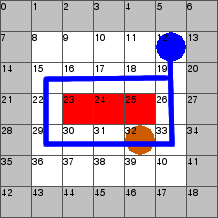
\includegraphics[scale=.33]{figs/7x7_liveness.png}
\begin{tikzpicture}[scale=0.9]
\draw[step=0.5cm,color=gray] (-1.5,-1.5) grid (1,1);
\filldraw[fill=blue,draw=black] (+0.75,+0.75) circle (0.2cm);
\filldraw[fill=red,draw=black] (0,0) rectangle (-0.5,-0.5);
\filldraw[fill=red,draw=black] (-0.5,0) rectangle (-1,-0.5);
\filldraw[fill=red,draw=black] (0,0) rectangle (0.5,-0.5);
\filldraw[fill=blue!40!white,draw=black] (+0.75,+0.75) circle (0.2cm);
\filldraw[fill=orange!40!white,draw=black] (0.25,-0.75) circle (0.2cm);
\draw[blue,thick] (-1.35,-0.75) rectangle (0.75,0.25);
\draw[blue,thick,->] (0.73,0.75) -> (0.75,0.25);
\node at (-1.30,+0.75) {\tiny{0}};
\node at (-0.80,+0.75) {\tiny{1}};
\node at (-0.30,+0.75) {\tiny{2}};
\node at (0.20,+0.75) {\tiny{3}};
\node at (0.73,+0.75) {\tiny{4}};
\node at (-1.35,+0.25) {\tiny{5}};
\node at (-0.85,+0.25) {\tiny{6}};
\node at (-0.35,+0.25) {\tiny{7}};
\node at (0.25,+0.25) {\tiny{8}};
\node at (0.75,+0.25) {\tiny{9}};
\node at (-1.35,-0.25) {\tiny{10}};
\node at (-0.85,-0.25) {\tiny{11}};
\node at (-0.35,-0.25) {\tiny{12}};
\node at (0.25,-0.25) {\tiny{13}};
\node at (0.75,-0.25) {\tiny{14}};
\node at (-1.35,-0.75) {\tiny{15}};
\node at (-0.85,-0.75) {\tiny{16}};
\node at (-0.35,-0.75) {\tiny{17}};
\node at (0.25,-0.75) {\tiny{18}};
\node at (0.75,-0.75) {\tiny{19}};
\node at (-1.35,-1.25) {\tiny{20}};
\node at (-0.85,-1.25) {\tiny{21}};
\node at (-0.35,-1.25) {\tiny{22}};
\node at (0.25,-1.25) {\tiny{23}};
\node at (0.75,-1.25) {\tiny{24}};
\end{tikzpicture}
\end{center}
\end{minipage}
\begin{minipage}{0.28\textwidth}
\vspace{0.1cm}
\caption{ Agent locations on an (infinite) path in the abstract counterexample graph from Example~\ref{ex:simple-liveness-counterex}. In the graph, the first node is labelled with $(4,\{18\})$, the second with $(9,\{Q_2\})$, and all other nodes with some $(l_a,\{Q_1,Q_2\})$.}
\label{fig:simple-liveness-counterex}
\end{minipage}

\end{figure}

\bigskip 

\begin{example}\label{ex:simple-liveness-counterex}
We saw in Example~\ref{ex:simple-safety-realizability} that in the safety surveillance game $(G,\LTLglobally p_2)$ the agent does not have a winning strategy. %This means, that the agent cannot ensure keeping at all times the uncertainty about the current position of the target to at most two positions.
We now consider a relaxed requirement, namely, that the uncertainty drops to at most $2$ infinitely often. We consider the liveness surveillance game 
$(G,\LTLglobally \LTLfinally p_2)$.

Let $\part = \{Q_1,Q_2\}$ be the partition from Example~\ref{ex:simple-safety-unconcretizable}. That is, $Q_1$, corresponds to the first two columns of the grid, and the set $Q_2$ contains the locations from the other three columns. 


Figure~\ref{fig:simple-liveness-counterex} shows an infinite path (in lasso form) in the abstract game $(\alpha_\part(G),\LTLglobally \LTLfinally p_2)$.  The figure depicts only the corresponding trajectory (sequence of positions) of the agent. The initial abstract state is $(4,\{18\})$, the second node on the path is labeled with the abstract state $(9,\{Q_2\})$, and all other nodes on the path are labeled with abstract states of the form $(l_a,\{Q_1,Q_2\})$ for some $l_a$. As each abstract state in the cycle violates $p_2$, the path violates $\LTLglobally \LTLfinally p_2$. The same holds for all infinite paths in the existing abstract counterexample graph.
\qed
\end{example}

\bigskip

A \emph{concrete counterexample graph} $\counterex_\belief$ for the belief game $(G_\belief,\LTLglobally\LTLfinally p_k)$ is defined analogously, with the difference that the nodes are now labelled with states in $S_\belief$.

An abstract counterexample graph $\counterex_\abstr$ for the game $(G_\abstr,\LTLglobally\LTLfinally p_k)$ is \emph{concretizable} if there exists a counterexample
$\counterex_\belief$ in $(G_\belief,\LTLglobally \LTLfinally p_k)$, such that for each infinite path $\pi_\abstr = v_\abstr^0,v_\abstr^1,\ldots$ starting from the initial node of $\counterex_\abstr$ there exists an infinite path $\pi_\belief = v_\belief^0,v_\belief^1,\ldots$ in $\counterex_\belief$ staring from its initial node such that if $v_\abstr^i$ is labelled with $(l_a,A_t)$ in $\counterex_\abstr$, then the corresponding node $v_\belief^i$ in $\counterex_\belief$ is labelled with $(l_a,B_t)$ for some $B_t \in \mathcal{P}(L)$ for which $B_t \subseteq \gamma(A_t)$.

Similarly to the set of trees associated with an abstract counterexample tree defined in the previous section, we can define a set of graphs $\graphs(\counterex_\abstr)$ of potential concretizations of $\counterex_\abstr$. In the remainder of this section we describe a procedure for constructing and analyzing one such graph, which will then have to be repeated for the different graphs.

Again, for the case of perfect sensing and no static sensors, the set of graphs contains a single graph. 
%\subsection{Counterexample-Guided Refinement}
%\subsubsection{Forward belief-set propagation}

To check if an abstract counterexample graph $\counterex_\abstr$ is concretizable, we construct a finite graph $\mathcal{D}$ whose nodes are labelled with elements of $\states_\belief$ and with nodes of $\counterex_\abstr$.
By construction we will ensure that if a node $d$ in $\mathcal D$ is labelled with $\langle(l_a,B_t),v \rangle$, where $(l_a,B_t)$ is a belief state, and $v$ is a node in $\counterex_\abstr$, then $v$ is labelled with $(l_a,A_t)$ in $\counterex_\abstr$, and $B_t \subseteq \gamma(A_t)$. 

Initially $\mathcal D$ contains a single node $d_0$ labelled with $\langle s_\belief^\init,v_0\rangle$, where $v_0$ is initial node of $\counterex_\abstr$. Consider a node $d$ in $\mathcal D$ labelled with $\langle(l_a,B_t),v \rangle$. For every child $v'$ of $v$ in $\counterex_\abstr$, labelled with an abstract state $(l_a',A_t')$ we proceed as follows. We select one belief set $B_t$ such that $((l_a,B_t),(l_a',B_t')) \in T_\belief$ and $B_t' \subseteq \gamma(A_t')$. If there exists a node $d'$ in $\mathcal D$ labelled with $\langle (l_a',B_t'),v\rangle$, then we add an edge from $d$ to $d'$ in $\mathcal{D}$. Otherwise, we create such a node and add the edge. We continue until no more nodes and edges can be added to $\mathcal D$. The procedure is guaranteed to terminate, since both  the graph $\counterex_\belief$, and $\states_\belief$ are finite, and we add a node labelled $\langle s_\belief, v\rangle$ to $\mathcal D$ at most once. Furthermore, the number of different graphs that we can construct in this way, by choosing different successor belief sets, is also finite. Thus, the set of graphs $\graphs(\counterex_\abstr)$ is also finite.

If every graph $\mathcal D$ in $\graphs(\counterex_\abstr)$ contains a reachable cycle (it suffices to consider simple cycles, i.e., without repeating intermediate nodes) $\rho = d_0,\ldots,d_n$ with $d_0 = d_n$ such that some $d_i$ is labelled with $(l_a,B_t)$ where $(l_a,B_t) \models p_k$, then we can conclude that the abstract counterexample $\counterex_\abstr$ is not concretizable. If for some graph $\mathcal D$ no such cycle exists, then $\mathcal D$ is a concrete counterexample graph for $(G_\belief,\LTLglobally\LTLfinally p_k)$. 

%\comment{
\begin{algorithm}[h!] 
%\small
%\vspace{-.5cm}
\KwIn{liveness surveillance game $(G,\LTLglobally\LTLfinally p_k)$, \newline 
abstract counterexample graph $\counterex_\abstr$ with initial node $v_0$}
\KwOut{a path $\pi$ in a graph $\mathcal D$ or {\sc concretizable}}

\smallskip

let $\mathcal D = (D,E)$ be a graph with\\
nodes $D := \{d_0\}$ and edges $E := \emptyset$\;

\smallskip

annotate $d_0$ with $\langle s_\belief^\init, v_0\rangle$\; 

\SetKwRepeat{Do}{do}{while}

\Do{$\mathcal D \neq \mathcal D'$}{
$\mathcal D' := \mathcal D$\;
 \ForEach{node $d$ in $\mathcal D$ labelled with $\langle(l_a,B_t),v\rangle$}{
  \ForEach{child $v'$ of $v$ in $\counterex_\abstr$ labelled $(l_a',A_t')$}{
  let $B_t$ be such that $B_t' \subseteq \gamma(A_t')$ and $((l_a,B_t),(l_a',B_t')) \in T_\belief$\;
  \eIf{there is a node $d' \in D$ labelled with $\langle (l_a',B_t'),v'\rangle$}{add an edge $(d,d')$ to $E$}
  {add a node $d'$ labelled $\langle (l_a',B_t'),v'\rangle$\;
  add an edge $(d,d')$ to $E$}
}
}
}
\leIf{there is a lasso path $\pi$ in $\mathcal D$ starting from $d_0$ such that some node in the cycle is annotated with $\langle s_\belief,v\rangle$ and $s_\belief\models p_k$}
{\KwRet{$\pi$;}\newline}
{\KwRet{{\sc concretizable}}}

\smallskip

\caption{Analysis of abstract counterexample graphs for games with liveness surveillance objectives.}
\label{algo:cex-analysis-liveness}
\end{algorithm}
%}


\bigskip 

\begin{example}\label{ex:simple-liveness-unconcretizable}
The abstract counterexample graph in the game $(\alpha_\part(G),\LTLglobally \LTLfinally p_2)$ discussed in Example~\ref{ex:simple-liveness-counterex} is not conretizable, since for the path in the abstract graph depicted in Figure~\ref{fig:simple-liveness-counterex} there exists a corresponding path in the unique graph $\mathcal D$ with a node in the cycle labelled with a set in $G_\belief$ that satisfies $p_2$. More precisely, the cycle in the graph $\mathcal D$ contains a node labelled with $(19,\{10\})$. Intuitively, as the agent moves from the upper to the lower part of the grid along this path, upon not observing the target, it can infer from the sequence of observations that the only possible location of the target is $10$. Thus, this infinite path is winning for the agent.
\qed
\end{example}

\bigskip 

\begin{theorem}
If for some graph $\mathcal{D}$ in $\graphs(\counterex_\abstr)$  Algorithm~\ref{algo:cex-analysis-liveness} returns {\sc concretizable}, then $\counterex_\abstr$ is concretizable. Otherwise, if for every graph $\mathcal D$ in $\graphs(\counterex_\abstr)$ it returns path $\pi$ in $\mathcal D$, then $\counterex_\abstr$ is not concretizable.
\end{theorem}
{\it Proof.}\ \ 
By applying Algorithm~\ref{algo:cex-analysis-liveness} in order to analyze all graphs in $\graphs(\counterex_\abstr)$, we check for each such graph if it is a concrete counterexample graph, that is, for each of its lasso paths the every state in the loop of that path violates $p_k$. By definition, Algorithm~\ref{algo:cex-analysis-liveness} returns {\sc concretizable} precisely when this is the case, that is when $\counterex_\abstr$ is concretizable. If for each graph in $\graphs(\counterex_\abstr)$ the algorithm returns a lasso path $\pi$ for which every state in its loop violates $p_k$, then this path demonstrates that the corresponding graph is not a concrete counterexample. If this is the case for all graphs in $\graphs(\counterex_\abstr)$, then $\counterex_\abstr$ is indeed spurious.
\qed

\bigskip 

\subsubsection{Backward partition splitting}

Consider a path in a graph $\mathcal{D}\in\graphs(\counterex_\abstr)$ of the form $\pi = d_0,\ldots, d_n,d_0',\ldots,d_m'$ where $d_n = d_m'$, and where for some $0 \leq i \leq m$ for the label $(l_a^i,B_t^i)$ it holds that $(l_a^i,B_t^i) \models p_k$. Let 
$\pi_\abstr = v_0,\ldots, v_n,v_0',\ldots,v_m'$ be the sequence of nodes in $\counterex_\abstr$ corresponding to the labels in $\pi$. By construction of $\mathcal D$, $\pi_\abstr$ is a path in $\counterex_\abstr$ and $v_n = v_m'$. We apply the refinement procedure from Algorithm~\ref{algo:refinement-safety} to the whole path $\pi_\abstr$, as well as to the path-prefix $v_0,\ldots, v_n$.


Let $\part$ and $\part'$ be two counterexample partitions such that $\part' \preceq \part$. Let $\counterex_\abstr$ be an abstract counterexample graph in $(\alpha_\part(G),\LTLglobally\LTLfinally p_k)$. We define $\gamma_{\part'}(\counterex_\abstr)$ to be the set of abstract counterexample graphs in $(\alpha_{\part'}(G),\LTLglobally\LTLfinally p_k)$ such that for every infinite path $\pi$ in $\counterex_\abstr'$ there exists an infinite path $\pi$ in $\counterex_\abstr$ such that for every node in $\pi'$ labelled with $(l_a,A_t')$ the corresponding node in $\counterex_\abstr$ is labelled with an abstract state $(l_a,A_t)$ such that $\gamma(A_t') \subseteq \gamma(A_t)$.


\bigskip 

\begin{theorem}If $\part'$ is the partition 
obtained by refining $\part$ with respect to all graphs in the set $\graphs(\counterex_\abstr)$ for an unconcretizable abstract counterexample $\counterex_\abstr$ in $(\alpha_\part(G),\LTLglobally\LTLfinally p_k)$, then $\gamma_{\part'}(\counterex_\abstr) = \emptyset$, and also $\gamma_{\part''}(\counterex_\abstr) = \emptyset$ for every partition $\part''$ with $\part'' \preceq \part'$.
\end{theorem}
{\it Proof.}\ \ 
Let $\part'$ be the partition obtained by refining $\part$ with respect to all the graphs in $\graphs(C_\abstr)$ for an unconcretizable abstract counterexample $\counterex_\abstr$ in $(\alpha_\part(G),\LTLglobally\LTLfinally p_k)$.

For every graph in $\graphs(C_\abstr)$ and corresponding infinite path $(l_a^0,B_t^0)(l_a^1,B_t^1)\ldots$ represented as lasso, with which we have refined the abstraction, every abstract partition $\part'' \preceq \part'$, and every infinite lasso path $(l_a^0,A_t^0) (l_a^1,A_t^1)\ldots$ in $\alpha_{\part''}(G)$ with $\alpha_{\part''}(B_t^i) = A_t^i$ we have that $\widetilde A_t^j \models p_k$ for infinitely many $j$. That is, the performed refinement ensures that in every finer abstraction, the abstraction of the paths with respect to which the partition was refined is precise enough to ensure that the safety property is not violated on this path.

Now, assume for the sake of contradiction that $\gamma_{\part''}(\counterex_\abstr) \neq \emptyset$, and let $\counterex_\abstr'' \in\gamma_{\part''}(\counterex_\abstr)$. By the definition of $\gamma$ and $\graphs$, we have that there exists a graph $D$ in $\graphs(\counterex_\abstr)$ that is also an element of $\graphs(\counterex_\abstr'')$. Thus, for some $(l_a^0,B_t^0)\ldots (l_a^m,B_t^m)$ in $D$ with respect to which we have refined the abstraction, it holds that $(l_a^0,\alpha_{\part''}(B_t^0)) (l_a^1,\alpha_{\part''}(B_t^1))\ldots$ is an infinite path represented as lasso in $\counterex_\abstr''$. By the property above, we have $\alpha(B_t^i)\models p_k$ for infinitely many $i$, which contradicts to the choice of $\counterex_\abstr''$ as a counterexample in $\alpha_{\part''}(G)$. This concludes the proof that $\gamma_{\part''}(\counterex_\abstr) = \emptyset$.
\qed
\bigskip 

\begin{example}\label{ex:simple-liveness-refinement}
We refine the abstraction partition $\part$ from Example~\ref{fig:simple-liveness-counterex} using the path identified in Example~\ref{ex:simple-liveness-counterex}, in order to eliminate the abstract counterexample. For this, following the refinement algorithm, we first split the set $Q_1$ into sets $Q_1' = \{10\}$ and $Q_2' = Q_1 \setminus \{10\}$, and let $Q_3' = Q_2$. However, since from some locations in $Q_2'$ and in $Q_3'$ the target can reach locations in $Q_2'$ and $Q_3'$, in order to eliminate the counterexample, we need to propagate the refinement backwards along the path and split $Q_2'$ and $Q_3'$ further. With that, we obtain an abstraction partition with $10$ sets, which is guaranteed to eliminate this abstract counterexample. In fact, in this example this abstraction turns out to be sufficiently precise to obtain a winning strategy for the agent.
\qed
\end{example}

%
%%%%%%%%%%%%%%%%%%%%%%%%%%%%%%%%%%%%%%%%%%%%%%%%%%%%%%%%%%%%%%%%%%%%%%%%%%%%%%%%%
%
\section{BELIEF REFINEMENT FOR GENERAL SPECIFICATIONS}% SURVEILLANCE OBJECTIVES}
%
%\subsection{General Surveillance and Task Specifications}
%We have described refinement procedures for safety and liveness surveillance objectives. If we are given a conjunction of such objectives, we first apply the refinement procedure for safety, and if no path for which we can refine is found, we then apply the refinenment procedure for liveness. 

In the general case, we check if the counterexample contains a state for which the concrete belief is a strict subset of the abstract one. If this is not the case, then the counterexample is concretizable, otherwise we refine the abstraction to make this belief precise. In the special case when we have a conjunction of a surveillance and task specifications, we first refine with respect to the surveillance objective as described above, and if this is not possible, with respect to such a node. Since the set of states in the game is finite, the iterative refinement will terminate, either with a concretizable counterexample, or with a surveillance strategy.  


%\begin{itemize}
%\item $\LTLglobally p_k \wedge \LTLglobally\LTLfinally p_l$: first check concretizability of all paths in the graph to states violating the safety constraints, if one is not concretizable then done, if all are concretizable, then apply method for liveness.
%\item General surveillance objectives: refine for some node where the true belief is more precise than the abstract one. not guaranteed to eliminate counterexample, but refinement loop guaranteed to still terminate since system is finite state and a proper split is done at each step. heuristics for identifying such nodes.
%\item $\varphi_{\mathit{surveillance}} \wedge \varphi_{\mathit{task}}$  if surveillance is a conjunction of safety and liveness, then in sequence: safety, liveness, task; otherwise as previous item.
%\item Full specification language: as for general surveillance.
%\end{itemize}

%\subsection{Discussion on Abstraction Refinement}
%As we have shown, the iterative abstraction refinement procedure we have described is guaranteed to terminate with either a winning strategy for the agent or with a concrete counterexample. In theory, a user can start with a very uninformed abstraction (for example, a trivial abstraction with one abstraction partition consisting of the entire state space), and the counterexample-guided refinement procedure will eventually terminate with an abstraction and a corresponding strategy. In practice, however, it is advisable to start with a suitably chosen informed abstraction, in order to reduce the number of necessary refinement iterations. In the next section we show some examples of user-provided abstractions which even require no refinement at all. Furthermore, user-provided abstractions are oftentimes 
more `intuitive' compared to the ones generated by the automated refinement procedure.

Ideally, constructing a suitable initial abstraction should be automated as well. However, abstractions are highly dependent on the sensor function and the structure of the environment. The process of generating initial abstractions based on automatically identified map features is on-going work. 
%%%%%%%%%%%%%%%%%%%%%%%%%%%%%%%%%%%%%%%%%%%%%%%%%%%%%%%%%%%%%%%%%%%%%%%%%%%%%%%%%
%
\section{EXPERIMENTAL EVALUATION ON GRIDWORLD}\label{sec:experiments}
In this section we report on the application of the proposed method for surveillance strategy synthesis on gridworld-based examples. The purpose of the experimental evaluation is to highlight the following key points:
\begin{itemize}
    \item The effect of different abstractions on the evolution of the belief sets of the agent.
    \item Sequences of abstractions resulting from automated abstraction refinement.
    \item The qualitative differences in the agent's behaviour resulting from surveillance strategies synthesized for different types of specifications.
\end{itemize}


We apply the \texttt{slugs} reactive synthesis tool~\cite{EhlersR16} to the abstract surveillance games in order to synthesize the surveillance strategies. The experiments were performed on an Intel i5-5300U 2.30 GHz CPU with 8 GB of RAM. 

\subsection{Effect of Abstractions on Belief}
The aim of this experiment is to illustrate the effect of different abstractions (generated using different abstraction partitions) on the evolution of belief sets. Naturally, the finer the abstraction, the slower the growth of the size of the belief set over time, and hence the easier it is to satisfy the specification. However, the increased precision of the abstraction comes at the cost of increased synthesis time. 

Figure~\ref{fig:case1} shows a gridworld divided into 7 abstraction partitions. The surveillance objective requires the agent to infinitely often know precisely the location of the target (either see it, or have a belief consisting of one cell). Additionally, it has to perform the task of patrolling (visiting infinitely often) the green 'goal' cell. Formally, the specification is $\LTLglobally\LTLfinally p_1 \wedge \LTLglobally\LTLfinally \mathit{goal}$. The agent can move up to 3 grid cells away at each step. The sensor mode, that is, the observation function, used here is 'line-of-sight' with a range of 5 cells. The agent cannot see through obstacles (shown in red) and cannot see farther than 5 cells away.  We assume in this example that we have perfect sensing i.e., when the target is sensed, the agent knows its true location. There are no static sensors. 


\begin{figure}
\subfloat[Gridworld with a user-provided abstraction partition with 7 sets, marked by the thick black lines. \label{fig:case1}]{
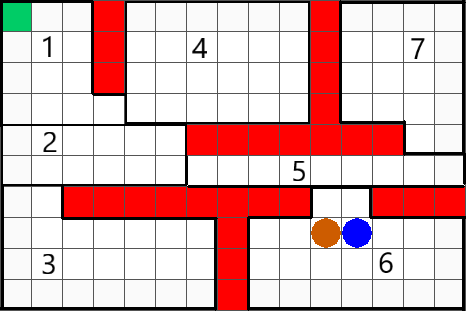
\includegraphics[width=0.45\linewidth]{Surveillance/figs/Liveness_part.png}
}
\hfill
\subfloat[Gridworld showing visibility of the agent. All locations shown in black are invisible to the agent. \label{fig:case1vis}]{
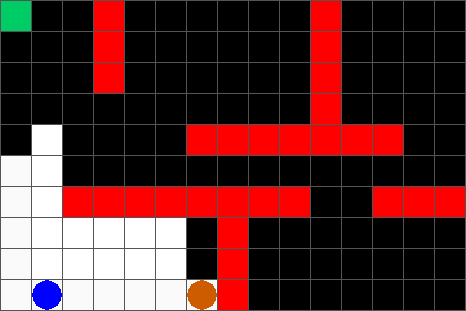
\includegraphics[width=0.45\linewidth]{Surveillance/figs/Liveness_t1.png}
}

\caption{10x15 gridworld with a liveness surveillance specification. The agent is depicted in blue, and the target in orange. The red locations are obstacles.}
\label{fig:casestudies1}

\end{figure}



\begin{figure}
\begin{minipage}{5.0cm}
	\centering
		\subfloat[$t_1$ \label{fig:case1t2}]{
		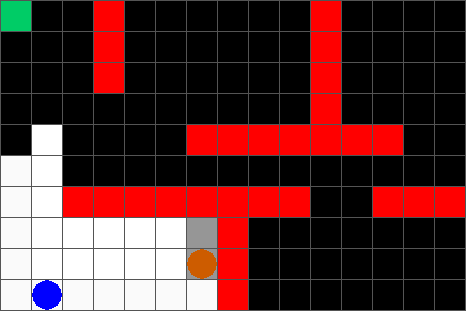
\includegraphics[width=0.47\linewidth]{Surveillance/figs/Liveness_t2.png}\hspace{.5cm}
	}
	\subfloat[$t_3$ \label{fig:case1t3}]{
		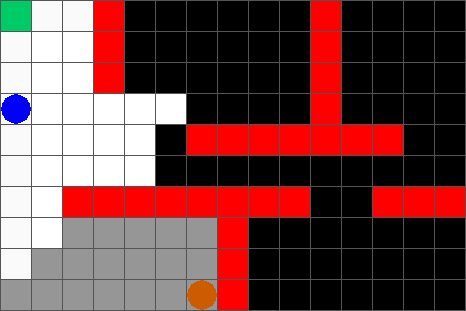
\includegraphics[width=0.47\linewidth]{Surveillance/figs/Liveness_t3.png}\hspace{.5cm}
	}
	\subfloat[$t_4$ \label{fig:case1t4}]{
	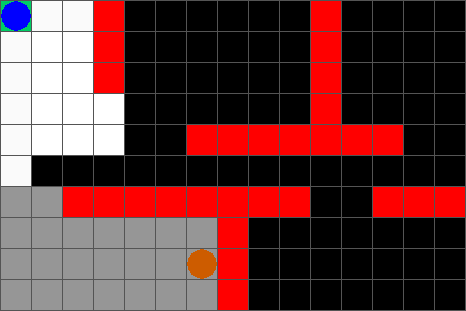
\includegraphics[width=0.47\linewidth]{Surveillance/figs/Liveness_t4.png}\hspace{.5cm}
}
\end{minipage}
\begin{minipage}{5.0cm}
	\centering
	\subfloat[$t_5$  \label{fig:case1t5}]{
		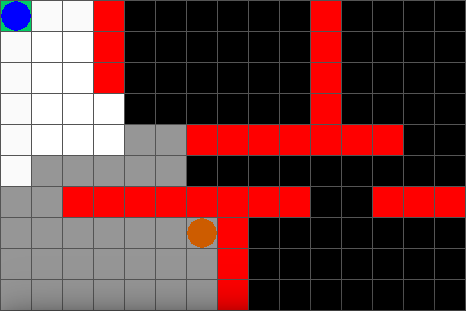
\includegraphics[width=0.47\linewidth]{Surveillance/figs/Liveness_t5.png}\hspace{.5cm}
	}
	\subfloat[$t_6$ \label{fig:case1t6}]{
		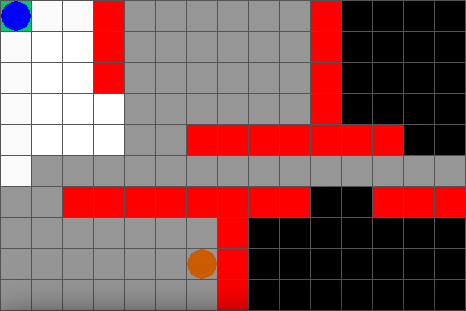
\includegraphics[width=0.47\linewidth]{Surveillance/figs/Liveness_t6.png}\hspace{.5cm}
	}
	\subfloat[$t_7$ \label{fig:case1t7}]{
		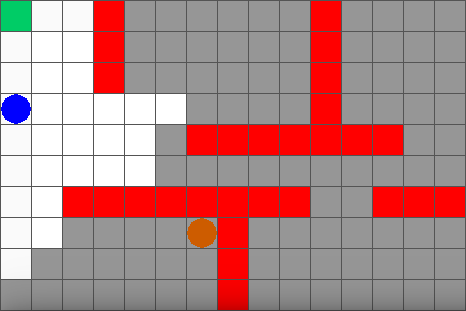
\includegraphics[width=0.47\linewidth]{Surveillance/figs/Liveness_t7.png}\hspace{.5cm}
	}
	
\end{minipage}

	
	\caption{Evolution of the agent's belief about the target's location as it moves towards the goal and loses sight of the target. Grey cells represent the locations the agent believes the target could be in. We show the belief at different timesteps $t_1,\ldots,t_7$ (note that $t_2$ is excluded for space concerns)
		}
	\label{fig:case1exp}
	
\end{figure}

Figure \ref{fig:case1exp} shows how the belief of the agent (shown in grey) can grow quickly when it cannot see the target. This growth occurs due to the coarseness of the abstraction, which overapproximates the target's true location. In 7 steps, the agent believes the target can be anywhere in the grid that is not in its vision. It has to then find the target in order to satisfy the surveillance requirement. Figure \ref{fig:search} illustrates the searching behaviour of the agent when it is trying to lower the belief below the threshold in order to satisfy the liveness specification. This  behaviour contrasts with the behaviour under safety surveillance considered later. A video of the simulation can be found at \url{http://goo.gl/YkFuxr}.

\begin{figure}

	\begin{minipage}{5.0cm}
		\centering
		\subfloat[$t_5$ \label{fig:search1}]{
			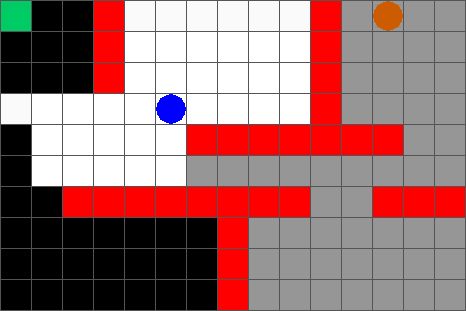
\includegraphics[width=0.47\linewidth]{Surveillance/figs/search_t2.png}\hspace{.5cm}
		}
		\subfloat[$t_7$ \label{fig:search2}]{
			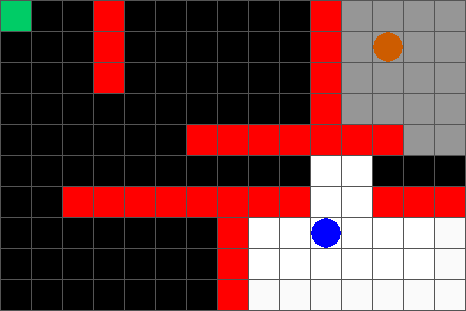
\includegraphics[width=0.47\linewidth]{Surveillance/figs/search_t3.png}\hspace{.5cm}
		}
		\subfloat[$t_9$ \label{fig:search3}]{
			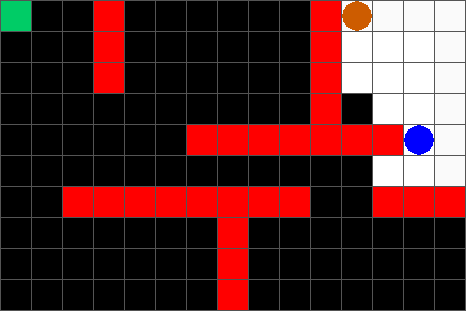
\includegraphics[width=0.47\linewidth]{Surveillance/figs/search_t4.png}\hspace{.5cm}
		}
	\end{minipage}
	\caption{The agent has to search for the target in order to lower its belief below the surveillance liveness specification.
	}
	\label{fig:search}
	
\end{figure}

In this example, an abstraction partition of size 7 was enough to guarantee the satisfaction of the surveillance specification.  For the purpose of comparison, we also solve the game with  an abstraction partition of size 12  to illustrate the change in belief growth. Figure \ref{fig:case1fineexp} shows the belief states growing much more slowly as the abstract belief states are smaller, and thus they more closely  approximate the true belief.
\begin{figure}

	\begin{minipage}{5.0cm}
		\centering
		\subfloat[$t_1$ \label{fig:casefine1t2}]{
			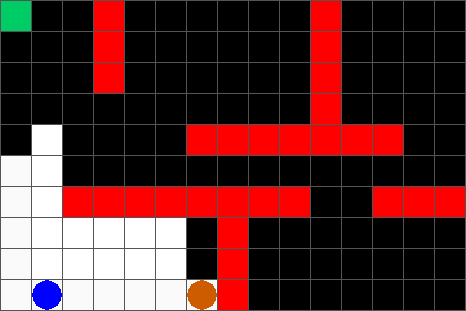
\includegraphics[width=0.47\linewidth]{Surveillance/figs/Liveness_t1.png}\hspace{.5cm}
		}
		\subfloat[$t_3$ \label{fig:case1finet3}]{
			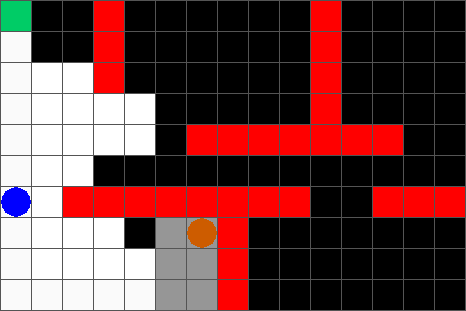
\includegraphics[width=0.47\linewidth]{Surveillance/figs/Liveness_fine_t11.png}\hspace{.5cm}
		}
		\subfloat[$t_4$ \label{fig:case1finet4}]{
			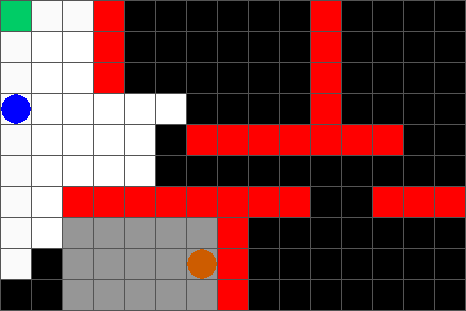
\includegraphics[width=0.47\linewidth]{Surveillance/figs/Liveness_fine_t2.png}\hspace{.5cm}
		}
	\end{minipage}
	\begin{minipage}{5.0cm}
		\centering
		\subfloat[$t_5$  \label{fig:case1finet5}]{
			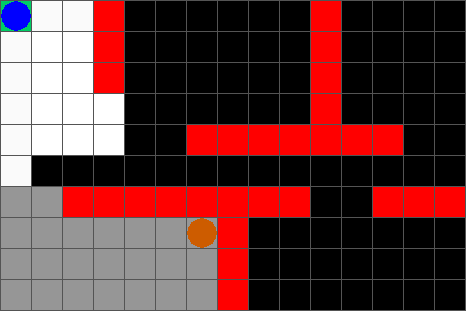
\includegraphics[width=0.47\linewidth]{Surveillance/figs/Liveness_fine_t3.png}\hspace{.5cm}
		}
		\subfloat[$t_6$ \label{fig:case1finet6}]{
			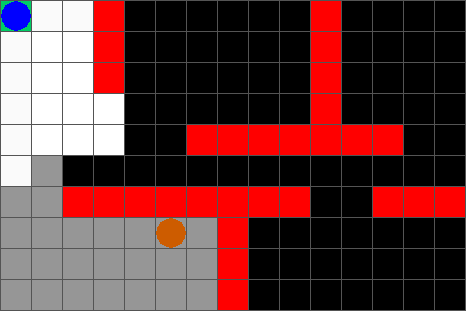
\includegraphics[width=0.47\linewidth]{Surveillance/figs/Liveness_fine_t4.png}\hspace{.5cm}
		}
		\subfloat[$t_7$ \label{fig:case1finet7}]{
			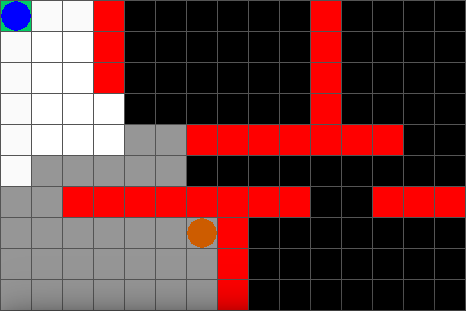
\includegraphics[width=0.47\linewidth]{Surveillance/figs/Liveness_t5.png}\hspace{.5cm}
		}
		
	\end{minipage}
	
	
	\caption{Evolution of the agent's belief about the target's location in a game  with an abstraction partition of size 12.
	}
	\label{fig:case1fineexp}
	
\end{figure}


The additional abstraction partitions result in a much larger game as the state space grows exponentially in the size of the abstraction partition. We compared the sizes of two abstract games for the 15x10 gridworld shown in Figure \ref{fig:casestudies1}, and the time it takes to synthesize a surveillance strategy in each of them. For an abstraction partition of size 7 the abstract game has 41700 states, and the synthesis time is 237s. In comparison, for an abstraction partition of size 13 the size of the abstract game is 636900 and the synthesis time is 810s. In contrast, the concrete belief-set game will have in the order of $2^{150}$ states, which is a state-space size that state-of-the-art synthesis tools cannot handle. 

%Table \ref{tab:exp1} compares the sizes of the corresponding abstract games, and the time it takes to synthesize a surveillance controller in each case.


%\begin{table}[h!]
%	\centering
%	\begin{tabular}{c|c|c}
%	Size of abstraction partition & Size of abstract game & Synthesis time \\ \hline \hline
%		7 & 41700 & 237s \\ 
%		12 & 636900 & 810s \\ 
%	\end{tabular}\caption{Comparison of synthesis times for coarse and fine abstractions on a 15x10 gridworld shown in Figure \ref{fig:casestudies}} \label{tab:exp1}
%\end{table}




\subsection{Automated Abstraction Refinement}
We now present an experiment to demonstrate the working of abstraction refinement procedure. 


\begin{figure}
\subfloat[User-provided initial abstraction. \label{fig:case1_autopart_before}]{\begin{tikzpicture}[scale=1]
\draw[step=0.5cm,color=gray] (-3.5,-2) grid (3,2);


\filldraw[fill=green,draw=black] (-3.5,2) rectangle (-3,1.5);
% \filldraw[fill=red,draw=black] (-2.5,2) rectangle (-2,1.5);
\filldraw[fill=red,draw=black] (-2.5,2) rectangle (-2,1.0);
\filldraw[fill=red,draw=black] (1,2) rectangle (1.5,0.0);
\filldraw[fill=red,draw=black] (-1,0.5) rectangle (2.5,0.0);
\filldraw[fill=red,draw=black] (2,-0.5) rectangle (3,-1.0);
\filldraw[fill=red,draw=black] (-2,-0.5) rectangle (1,-1.0);
\filldraw[fill=red,draw=black] (-0.5,-1.0) rectangle (0,-2.0);

\filldraw[fill=none,draw=blue,line width=0.6mm] (-3.5,2.0) rectangle (-2.5,-2.0);
\draw[black, line width = 0.6mm] plot coordinates{(-2.0,2) (-2.0,1) (-2.5,1) (-2.5,-2) (-0.5,-2) (-0.5,-1) (-2.0,-1) (-2.0,-0.5) (3.0,-0.5) (3.0,-0.0) (-1.0,-0.0) (-1.0,0.5) (1.0,0.5) (1.0,2)}--cycle;
\draw[cyan, line width = 0.6mm] plot coordinates{(0,-1.0) (0,-2.0) (3,-2.0) (3,-1.0) (2,-1.0) (2,-0.5) (1,-0.5) (1,-1.0)}--cycle;
\draw[magenta, line width = 0.6mm] plot coordinates{(1.5,2.0) (1.5,0.5) (2.5,0.5) (2.5,0.0) (3.0,0.0) (3.0,2.0)}--cycle;
% \filldraw[fill=blue!40!white,draw=black] (+0.75,+0.75) circle (0.2cm);
% \filldraw[fill=orange!40!white,draw=black] (0.25,-0.75) circle (0.2cm);
\node at (-3.0,+0.0) {\normalsize{\textbf{$Q_1$}}};
\node at (-1.5,-0.0) {\normalsize{\textbf{$Q_2$}}};
\node at (2.25,1.25) {\normalsize{\textbf{$Q_3$}}};
\node at (1.5,-1.5) {\normalsize{\textbf{$Q_4$}}};
% \node at (-1.5,-0.0) {\large{\textbf{2}}};
% \node at (-0.30,+0.75) {\tiny{2}};
% \node at (0.20,+0.75) {\tiny{3}};
% \node at (0.73,+0.75) {\tiny{4}};
% \node at (-1.33,+0.25) {\tiny{5}};
% \node at (-0.85,+0.25) {\tiny{6}};
% \node at (-0.35,+0.25) {\tiny{7}};
% \node at (0.25,+0.25) {\tiny{8}};
% \node at (0.75,+0.25) {\tiny{9}};
% \node at (-1.28,-0.27) {\tiny{10}};
% \node at (-0.78,-0.27) {\tiny{11}};
% \node at (-0.28,-0.27) {\tiny{12}};
% \node at (0.28,-0.27) {\tiny{13}};
% \node at (0.75,-0.25) {\tiny{14}};
% \node at (-1.3,-0.75) {\tiny{15}};
% \node at (-0.8,-0.75) {\tiny{16}};
% \node at (-0.3,-0.75) {\tiny{17}};
% \node at (0.25,-0.75) {\tiny{18}};
% \node at (0.75,-0.75) {\tiny{19}};
% \node at (-1.27,-1.25) {\tiny{20}};
% \node at (-0.8,-1.25) {\tiny{21}};
% \node at (-0.3,-1.25) {\tiny{22}};
% \node at (0.25,-1.25) {\tiny{23}};
% \node at (0.75,-1.25) {\tiny{24}};
\end{tikzpicture}}
%\hfill
\subfloat[Refined abstraction.\label{fig:refined-abstraction}]{
\begin{tikzpicture}[scale=1]
\draw[step=0.5cm,color=gray] (-3.5,-2) grid (3,2);


\filldraw[fill=green,draw=black] (-3.5,2) rectangle (-3,1.5);
% \filldraw[fill=red,draw=black] (-2.5,2) rectangle (-2,1.5);
\filldraw[fill=red,draw=black] (-2.5,2) rectangle (-2,1.0);
\filldraw[fill=red,draw=black] (1,2) rectangle (1.5,0.0);
\filldraw[fill=red,draw=black] (-1,0.5) rectangle (2.5,0.0);
\filldraw[fill=red,draw=black] (2,-0.5) rectangle (3,-1.0);
\filldraw[fill=red,draw=black] (-2,-0.5) rectangle (1,-1.0);
\filldraw[fill=red,draw=black] (-0.5,-1.0) rectangle (0,-2.0);

\filldraw[fill=none,draw=blue,line width=0.6mm] (-3.5,2.0) rectangle (-2.5,-2.0);
\draw[black, line width = 0.6mm] plot coordinates{(-2.0,2) (-2.0,1) (-2.5,1) (-2.5,-2) (-0.5,-2) (-0.5,-1) (-2.0,-1) (-2.0,-0.0) (-1.0,-0.0) (-1.0,0.5) (1.0,0.5) (1.0,2)}--cycle;
\draw[cyan, line width = 0.6mm] plot coordinates{(0,-1.0) (0,-2.0) (3,-2.0) (3,-1.0) (2,-1.0) (2,-0.5) (1,-0.5) (1,-1.0)}--cycle;


\filldraw[fill=none,draw=teal, line width=0.6mm] (-2.0,0.0) rectangle (-0.0,-0.5);
\filldraw[fill=none,draw=violet, line width=0.6mm] (-0.0,0.0) rectangle (1.0,-0.5);
\filldraw[fill=none,draw=lime, line width=0.6mm] (1.0,0.0) rectangle (3.0,-0.5);
\draw[brown, line width = 0.6mm] plot coordinates{(2.0,2.0) (2.0,1.0) (2.5,1.0) (2.5,0.0) (3.0,0.0) (3.0,2.0)}--cycle;
\draw[gray, line width = 0.6mm] plot coordinates{(1.5,2.0) (1.5,0.5) (2.5,0.5) (2.5,1.0) (2.0,1.0) (2.0,2.0)}--cycle;
\draw[darkgray, line width = 0.6mm] plot coordinates{(2.0,-1.0) (2.0,-1.5) (2.5,-1.5) (2.5,-2.0) (3,-2.0) (3,-1)}--cycle;


% \filldraw[fill=blue!40!white,draw=black] (+0.75,+0.75) circle (0.2cm);
% \filldraw[fill=orange!40!white,draw=black] (0.25,-0.75) circle (0.2cm);
\node at (-3.0,+0.0) {\textbf{$Q_1$}};
\node at (-1.25,-0.25) {\normalsize{\textbf{$Q_3$}}};
\node at (-1.0,1.25) {\normalsize{\textbf{$Q_2$}}};
\node at (1.5,-1.5) {\normalsize{\textbf{$Q_8$}}};
\node at (0.5,-0.25) {\normalsize{\textbf{$Q_4$}}};
\node at (2.0,-0.25) {\normalsize{\textbf{$Q_5$}}};
\node at (1.8,0.75) {\normalsize{\textbf{$Q_6$}}};
\node at (2.75,1.25) {\normalsize{\textbf{$Q_7$}}};
\node at (2.5,-1.25) {\normalsize{\textbf{$Q_9$}}};
% \node at (-1.5,-0.0) {\large{\textbf{2}}};
% \node at (-0.30,+0.75) {\tiny{2}};
% \node at (0.20,+0.75) {\tiny{3}};
% \node at (0.73,+0.75) {\tiny{4}};
% \node at (-1.33,+0.25) {\tiny{5}};
% \node at (-0.85,+0.25) {\tiny{6}};
% \node at (-0.35,+0.25) {\tiny{7}};
% \node at (0.25,+0.25) {\tiny{8}};
% \node at (0.75,+0.25) {\tiny{9}};
% \node at (-1.28,-0.27) {\tiny{10}};
% \node at (-0.78,-0.27) {\tiny{11}};
% \node at (-0.28,-0.27) {\tiny{12}};
% \node at (0.28,-0.27) {\tiny{13}};
% \node at (0.75,-0.25) {\tiny{14}};
% \node at (-1.3,-0.75) {\tiny{15}};
% \node at (-0.8,-0.75) {\tiny{16}};
% \node at (-0.3,-0.75) {\tiny{17}};
% \node at (0.25,-0.75) {\tiny{18}};
% \node at (0.75,-0.75) {\tiny{19}};
% \node at (-1.27,-1.25) {\tiny{20}};
% \node at (-0.8,-1.25) {\tiny{21}};
% \node at (-0.3,-1.25) {\tiny{22}};
% \node at (0.25,-1.25) {\tiny{23}};
% \node at (0.75,-1.25) {\tiny{24}};
\end{tikzpicture}
}
\caption{Experiment showcasing automated abstraction refinement in a 13$\times$8 gridworld. The user-provided abstraction of 4 abstract states shown in ~\ref{fig:case1_autopart_before} is refined further into 9 abstract states shown in~\ref{fig:refined-abstraction}.}
\label{fig:case1_autopart}
\end{figure}



Starting with an abstract game generated by a partition with four elements shown in Figure~\ref{fig:case1_autopart_before}, the refinement algorithm terminates after 5 iterations (with total running time of 821 s). The resulting partition $\mathcal{Q} = \{Q_1,...,Q_9 \}$ has $9$ elements shown as the numbered regions in Figure~\ref{fig:refined-abstraction}.

This experiment shows that, in general, we do not guarantee that the abstraction generated by the refinement approach is necessarily the smallest possible. A handcrafted partitioning in the same environment shown in the previous section was able to produce a winning strategy with 7 abstract belief states instead of 9. Although the abstraction refinement algorithm is always guaranteed to terminate, in general, the user-provided initial abstraction has a significant effect on the number of abstract belief states of the resulting abstraction. It is thus important to combine initial user-provided abstractions, that are crafted as well as possible, with the automated refinement that eliminates any remaining imprecision that was not accounted for by the user.

 



%\Suda{Not sure if we should keep this next part}
\subsection{Discussion}
 The difference in the behaviour in the case studies highlights the different use cases of the surveillance objectives. Depending on the domain, the user can specify a combination of safety and liveness specification to tune the behaviour of the agent. In a critical surveillance situation (typical in defense or security situations), the safety specification will guarantee to the user that the belief will never grow too large. However, in less critical situations (such as luggage carrying robots in airports), the robot has more flexibility in allowing the belief to grow as long as it can guarantee its reduction in the future. 
%
%%%%%%%%%%%%%%%%%%%%%%%%%%%%%%%%%%%%%%%%%%%%%%%%%%%%%%%%%%%%%%%%%%%%%%%%%%%%%%%%%
%
\section{SECURITY APPLICATION CASE STUDY}
%
In this section, we demonstrate the effectiveness of the proposed framework to a case study for an urban security application with high-fidelity simulated sensors and robots. 
%Physical security applications typically require the housing and protection of sensitive materials or locations. Often, such environments are large and it is difficult to have complete surveillance coverage at all times using only static sensors. In such situations, deploying an autonomous mobile agent with sensing capabilities can greatly reduce coverage requirements from static sensors. When utilizing autonomous agents it is necessary to provide quantitative guarantees on their belief of the location of an intruding target in order to direct security measures accurately. The method proposed in this paper generates strategies for fully autonomous surveillance with quantitative guarantees on the size of the belief of the target's location and hence is a natural fit for security applications. 
We provide the code for the implementation on Github\footnote{Github: \url{https://github.com/u-t-autonomous/Surveillance}} and the videos for all simulations at the corresponding Github page \footnote{Github page: \url{https://u-t-autonomous.github.io/Surveillance-Synthesis/}}.
%We will use the case study to demonstrate the versatility and applicability of our surveillance strategy and belief abstraction methods across multiple high-fidelity simulation environments.

% \subsection{Combating poaching}
% First, consider the problem of tracking poachers in Africa. 
% UAVs are increasingly being adopted for monitoring of illegal hunting and poaching \cite{poaching}. In countries such as Kenya \cite{poaching}, South Africa, and Zimbabwe \cite{drones}, drones have been deployed and tested in an attempt to reduce poaching by providing constant surveillance \cite{poaching}. However, all of these solutions still require a pilot to remotely operate the UAV or manually provide it waypoints. In this paper we propose a method to generate strategies that can allow for \emph{fully autonomous surveillance} with quantitative guarantees on the \emph{belief in the position of the target}. These quantitative guarantees allow a response to be effectively mobilized by relevant authorities. 

% We simulate a jungle environment using Unreal Engine 4 as shown in Figure \ref{fig:UE4JungleProto} and UAVs are simulated in the environment using an Airsim plugin \cite{airsim}. In Section VII we present simulations of an autonomous UAV performing surveillance mission in this environment. 

% \begin{figure}[h]
%     \centering
%     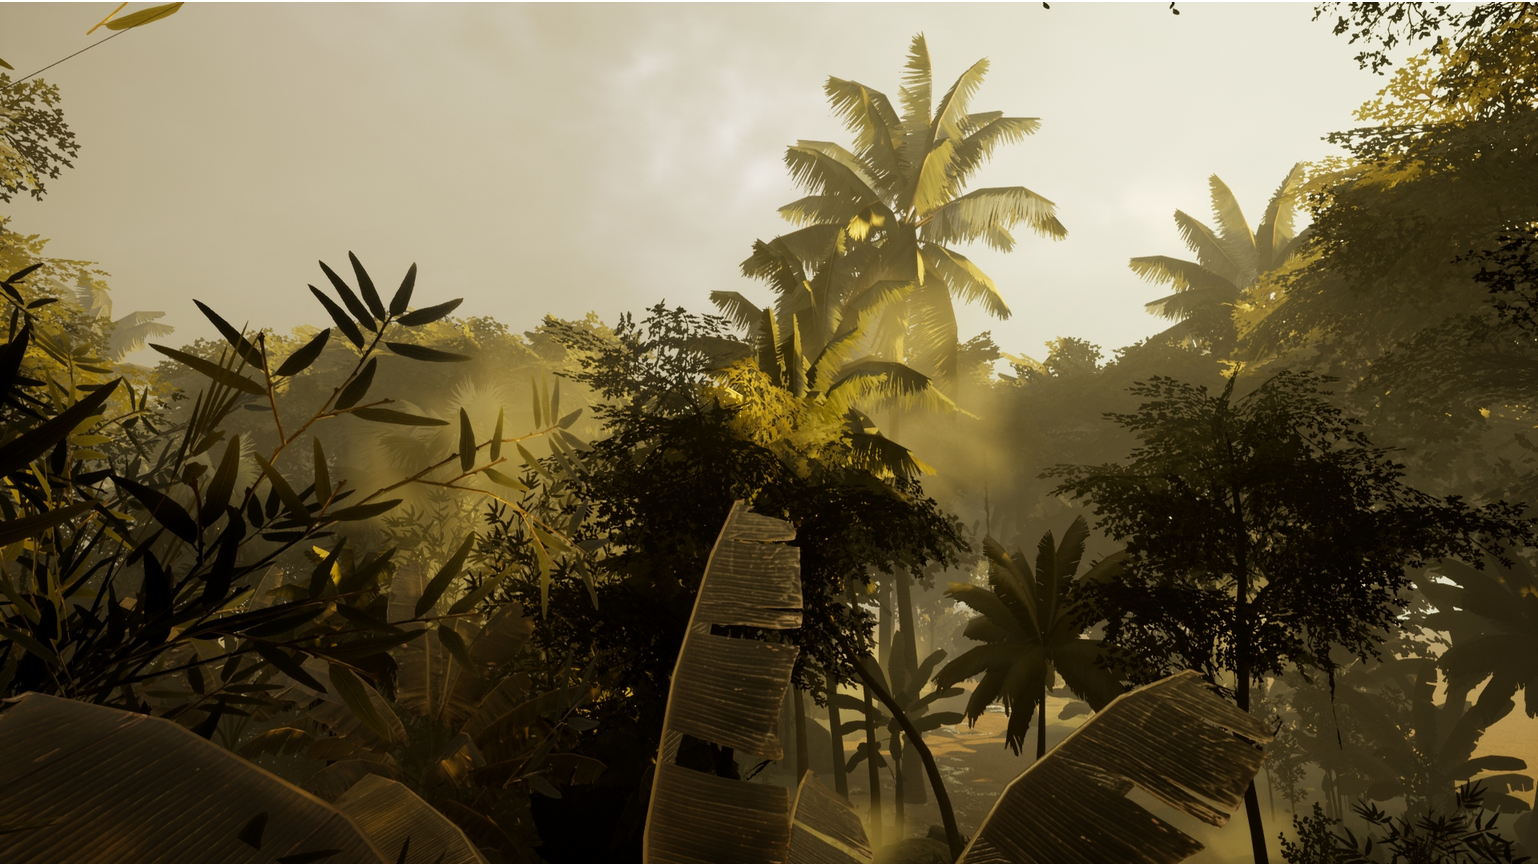
\includegraphics[width = 0.9\linewidth]{figs/UE4JungleProto.png}
%     \caption{Unreal Engine 4 Jungle Environment}
%     \label{fig:UE4JungleProto}
% \end{figure}
%\subsection{Security}



% \begin{figure}[h]
%     \centering
%     \includegraphics[width = 3 in]{figs/GazArena.png}
%     \caption{Gazebo Environment}
%     \label{fig:GazArena}
% \end{figure}

%andia National Labs considers examples where there is a compound that has a sensitive area that must be protected and is surrounded by land that contains wild life. Sometimes when an intruder is detected, the security system cannot determine if the threat is real or if there is simply an animal wandering around. A security officer must then go out and find the intruder to determine the state of the threat. In order to reduce wasted time, actively tracking that threat to provide the security personnel with a small region to search instead of a last known location saves resources. 

%and of security around a sensitive compound where tracking potential intruders is required for security personnel to make contact with and determine if the threat is real or false.




\subsection{Robot Platforms}

We use two robot simulation platforms to demonstrate the generality and applicability of the platform-agnostic methodology developed in this paper:
\begin{enumerate}
    \item An Iris quadcopter, which uses the PX4 flight stack and is capable of waypoint control.
    \item Stanley Innovations segway, which uses the ROS navigation stack for mapping, waypoint control, and autonomous obstacle avoidance. 
\end{enumerate}
To simulate the sensor output, we directly access the ground truth position of the moving target and add noise. We model the sensor and state estimation uncertainty as described in section \ref{sec:sensefunction} using a simulated 360 degree LiDAR with range of  $10$ meters, angular resolution of 1 degree, range accuracy of $\pm 3$ cm.


The function $vis$ is built directly from the sensor range parameter. To construct the function $sense$ we use a worst-case conservative Gaussian noise model. Given a sensor measurement, let $0 \leq p(l) \leq 1$ be the probability the target is in location $l$. We construct the uncertainty set $U$ of possible target states for each sensor measurement $sense(l_a,l_t)$ by including all states with a probability greater than $\delta$ where $0\leq \delta \leq 1$ can be set by the user. In the following simulations, we use $\delta = 0.95$. Informally, if a target is in sensor range, the agent's belief consists of \emph{all states} at which the target is with a probability greater than or equal to $5\%$. We note that, since the function $obs$ depends only on the sensors, the function needs to be constructed only once and can be used for all robots that use the same sensors. 
We test the synthesized surveillance strategies synthesized in two environments. One is an open urban-like setting modelled in Unreal Engine 4 depicted in Figure \ref{fig:UE4city}. A quadcopter acts as the surveilling agent and another acts as a potential intruder. In the second scenario, we consider an enclosed compound-like environment modelled in Gazebo as shown in Figure \ref{fig:GazArena}. The Iris quadcopter is tasked with tracking a hostile target (the Stanley Innovations segway) and maintaining sufficient knowledge of its location. We allow a human to directly control the rover and demonstrate the corresponding real-time response of the quadcopter to satisfy its surveillance task. We also perform the same experiment with the quadcopter controlled by a human and the Segway as the autonomous surveilling agent to emphasise that the framework is agnostic to the specific underlying hardware and can be easily applied. 
  
We contrast the surveillance needs and the qualitatively different resulting behaviours of the synthesized strategies for the agents in these two environments.

\begin{figure}
\centering


\subfloat[Urban environment modeled in Unreal Engine 4 \label{fig:UE4city}]{
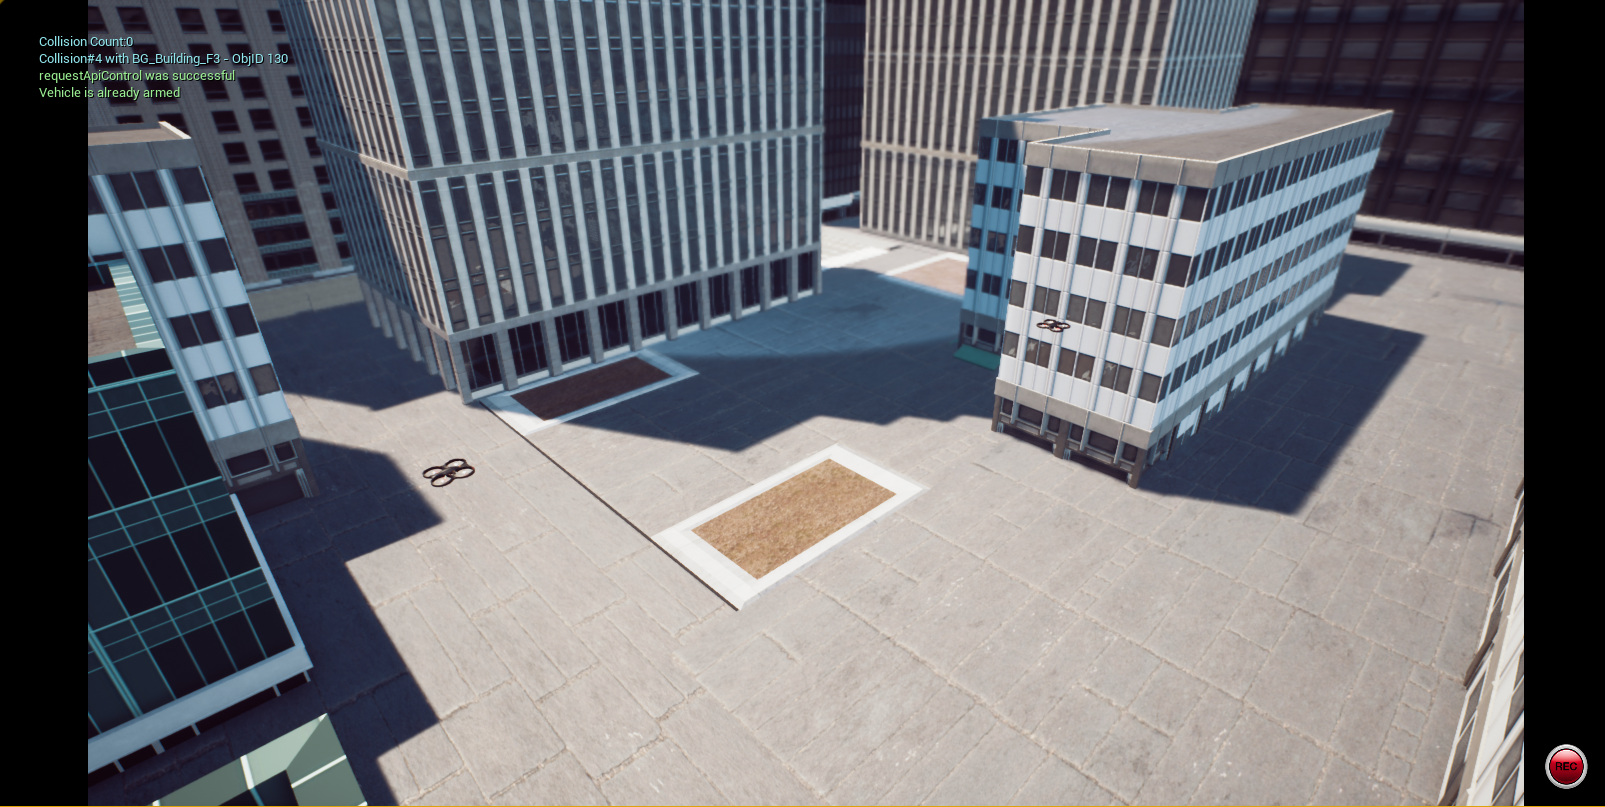
\includegraphics[width = 0.9\linewidth]{Surveillance/figs/unreal_city.png}}

\subfloat[Enclosed compound modelled in Gazebo \label{fig:GazArena}]{
\includegraphics[width = 0.9\linewidth]{Surveillance/figs/GazArena.png}}

\subfloat[Iris quadcopter used for autonomous surveillance \label{fig:sandiauav}]{
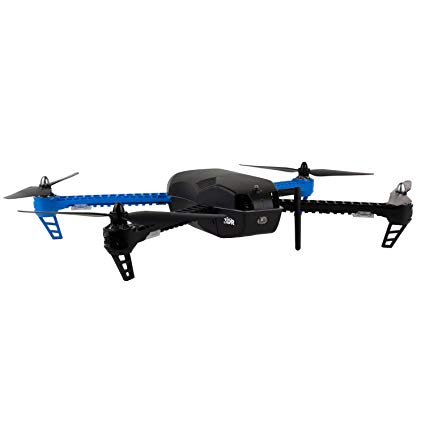
\includegraphics[width = 0.43\linewidth]{Surveillance/figs/quad.jpg}
} \hspace{0.05\linewidth}
\subfloat[Stanley innovations segway vehicle acting as a hostile target \label{fig:stanleyrobot}]{
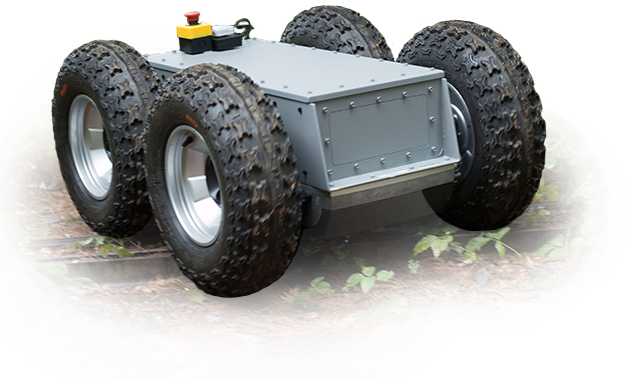
\includegraphics[width = 0.43\linewidth]{Surveillance/figs/Rugged-All-Terrain.png}
}

\caption{Case study for a security application. The vehicles are simulated in either Gazebo environment shown in \ref{fig:GazArena} or a UE4 environment shown in \ref{fig:GazArena}. A user can act as an `intruder' by controlling a target \ref{fig:stanleyrobot}. The UAV in \ref{fig:sandiauav} must autonomously react to guarantee the surveillance mission is satisfied. }
\label{fig:SandiaCaseSTudy}
\end{figure}
\subsection{Safety Surveillance Specification}
 In this example, we demonstrate the behaviour of the agent under a safety surveillance specification. We do so in the urban environment illustrated in Figure~\ref{fig:UE4city}. 
 
\begin{figure}
\centering
\subfloat[Top-down view of environment from Figure \ref{fig:UE4city}. The red square corresponds to the area in which the simulation takes place. \label{fig:topdownviewAirsim}]{
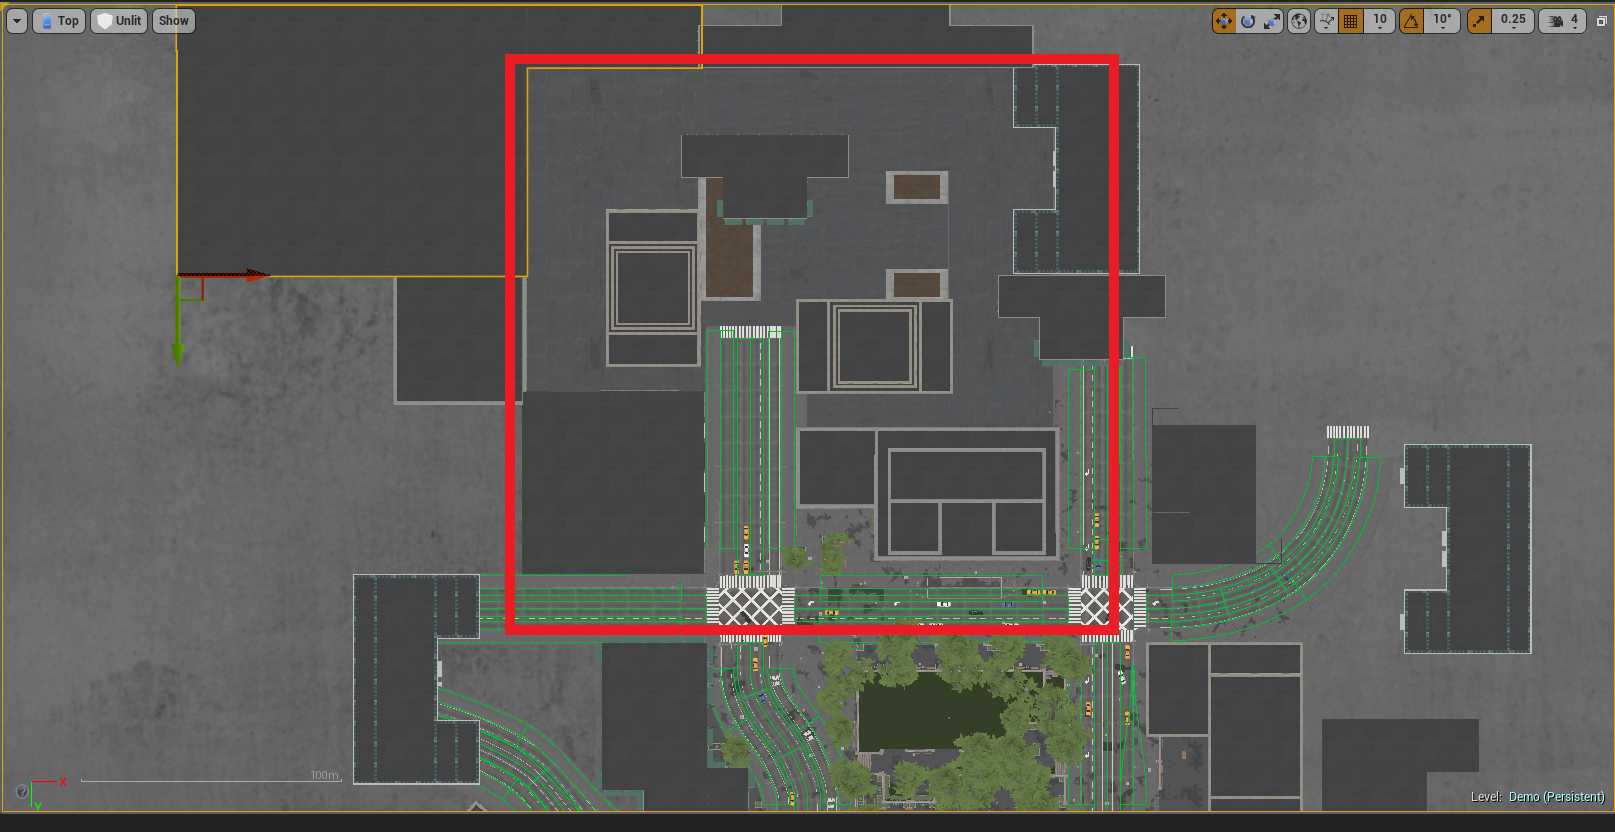
\includegraphics[width = 0.95\linewidth]{Surveillance/figs/downtown_map.png}}

\subfloat[The environment in \ref{fig:UE4city} is discretized into a 24x37 grid. Black cells are states that cannot be sensed from the current location of the agent. The agent is shown in blue, the evading target in orange. \label{fig:Airsim_grid}]{
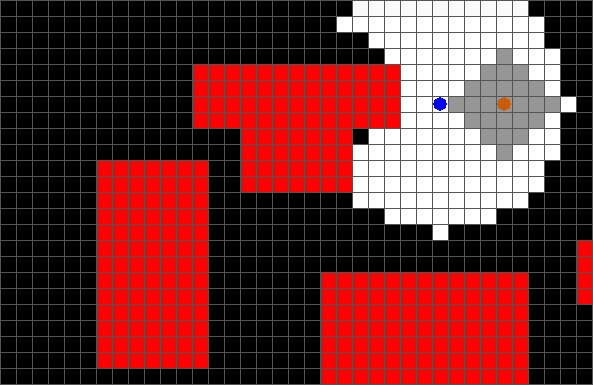
\includegraphics[width = 0.9\linewidth]{Surveillance/figs/Airsim_gridAirsim_Example.png}
}

\caption{The urban environment in Figure \ref{fig:GazArena} is discretized in \ref{fig:Airsim_grid} for synthesis. Note that due to the sensor uncertainty, the agent does not know the exact location of the target even when it is in range of its sensors.}
\label{fig:Airsim_casestudy}
\end{figure}
Figure~\ref{fig:Airsim_casestudy} depicts the top-down view environment created in \emph{Unreal Engine 4} and discretized for synthesis. The uncertainty in the sensing capaiblities of the agent is shown in Figure~\ref{fig:Airsim_grid} where grey cells correspond to the agent's current belief of the target's location stemming from the sensor and target state estimation uncertainty. The agent is 3 times faster than the target (it can move 3 cells for every 1 cell the target moves). 

In this setting, we require the satisfaction of the safety surveillance objective $\square p_{25}$ (the belief size should never exceed 25). In this case, we only need an abstraction with a trivial abstraction partition, consisting of the whole set of locations, as the agent has a strategy to closely follow and maintain view of the target. This is, in fact, necessary, as
any belief state will already be violating the safety requirement due to the estimation uncertainty. We are able to synthesize a strategy in 112 seconds. 
 
We present a video from the first-person view of the surveilling drone at \url{https://www.youtube.com/watch?v=HLsZ5ZnQgAg}. We note that the agent follows the target closely and never allows the target to leave its line of sight. In general, open urban environments the one considered here require stricter surveillance specifications as it is much harder to `find' a target once it has been lost. This will be in contrast with the more enclosed locations which we consider in the next case study.




\subsection{Liveness Surveillance Specification and Task Requirement} 
In this experiment, we demonstrate the behaviour an automatically synthesized strategy for the surveillance agent under a liveness surveillance specification and a task requirement. We do so in the Gazebo environment shown in Figure~\ref{fig:GazArena}. We compare this to a strategy for a safety surveillance specification with no additional task requirement, synthesized for the same environment. 



\begin{figure}
\subfloat[Lidar generated map of the gazebo environment in Figure~\ref{fig:GazArena}. \label{fig:Q_building_2}]{
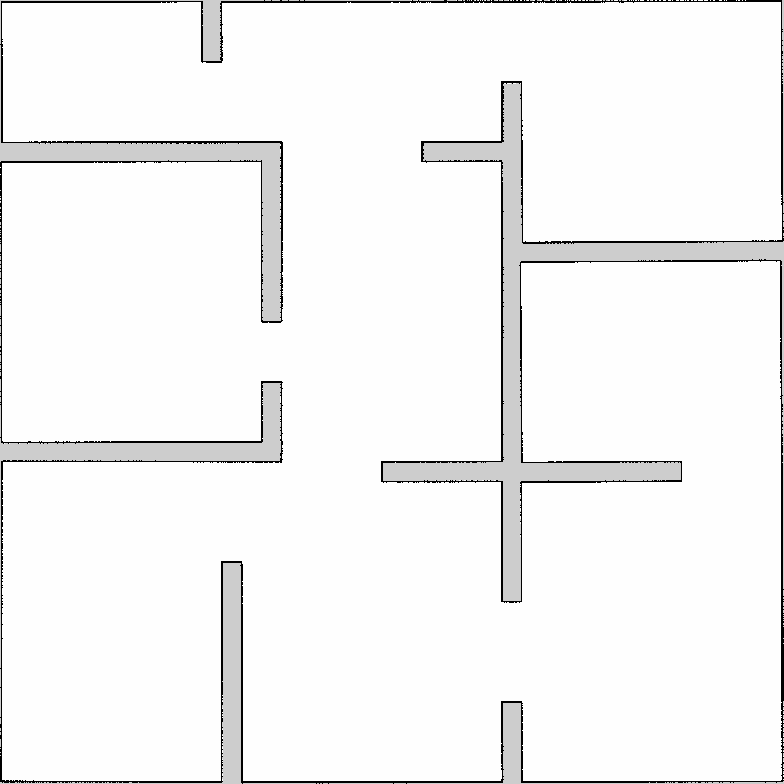
\includegraphics[width=0.45\linewidth]{Surveillance/figs/Q_building_2.png}
}
\hspace{0.5cm}
\subfloat[Discretization of the map \newline in Figure~\ref{fig:Q_building_2} used for synthesis \label{fig:gazebogrid}]{
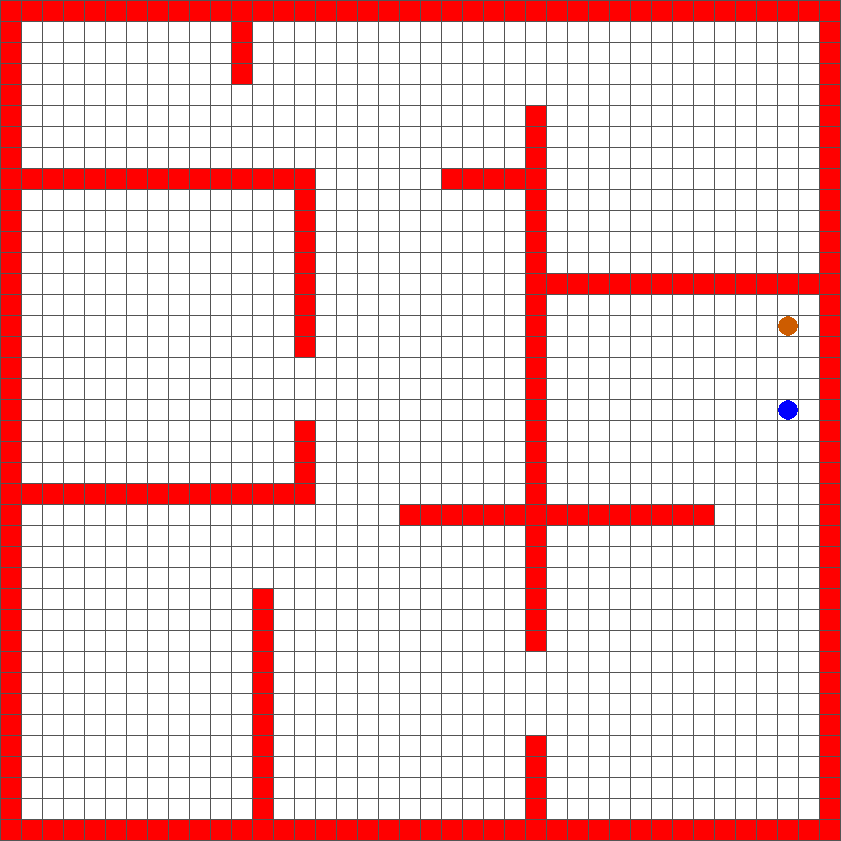
\includegraphics[width=0.45\linewidth]{Surveillance/figs/ROS_grid.png}\hspace{.5cm}
}

\caption{The Gazebo environment in Figure \ref{fig:GazArena} is first mapped using a LIDAR equipped agent to produce the map in~\ref{fig:Q_building_2} and then discretized to produce the gridworld in~\ref{fig:gazebogrid}.}
\label{fig:casestudiesros}

\end{figure}


The Iris quadcoptor shown in Figure~\ref{fig:sandiauav} is the agent being controlled by the synthesized surveillance strategy, and the Stanley Innovations Segway in Figure~\ref{fig:stanleyrobot} is the target. The target can either be controlled through a Python API or joystick such as an XBOX 360 controller. The quadcoptor uses a minimum snap trajectory package to plan its path, and a standard PX4 flight stack for the lower level flight control \cite{px4}. As in the previous section, we assume that the quadcoptor can move 3 times faster than the segway.

\begin{figure}[h]
  \definecolor{bg}{HTML}{ddeedd}
\definecolor{comp}{HTML}{c2d4dd}
\definecolor{impl}{HTML}{b0aac0}
\definecolor{ligb}{HTML}{5E7FC6}
\definecolor{bodybl}{HTML}{85A1DC}
\definecolor{headbl}{HTML}{264C9C}
\definecolor{bgyel}{HTML}{FFDC6B}
\definecolor{bodyyel}{HTML}{FFE58F}
\definecolor{headyel}{HTML}{E9BB25}
\definecolor{gr1}{HTML}{00FF00}
\definecolor{or1}{HTML}{FFAA00}
\definecolor{ye1}{HTML}{FFFF00}

% Define block styles
\tikzstyle{decision} = [diamond, draw, fill=blue!20, 
text width=4.5em, text badly centered, node distance=3cm, inner sep=0pt]
\tikzstyle{block} = [rectangle, draw, fill=blue!20, 
text width=5em, text centered, rounded corners, minimum height=4em]
\tikzstyle{line} = [draw, -latex']
\tikzstyle{cloud} = [draw, ellipse,fill=red!20, node distance=3cm,
minimum height=2em]
\def\checkmark{\tikz\fill[scale=0.6](0,.35) -- (.25,0) -- (1,.7) -- (.25,.15) -- cycle;} 
%
\centering
\begin{tikzpicture}[every node/.style={draw, text centered, shape=rectangle, rounded corners, text width=3cm, minimum height=0.8cm, inner sep=5pt}]
%\tikzstyle{outer}= [draw, text centered, shape=rectangle, text width=2cm, minimum height=1cm]
%\tikzstyle{inner}=[draw, text centered, shape=rectangle, rounded corners, text width=3.8cm, minimum height=1.1cm, inner sep=5pt]
\tikzstyle{decision} = [diamond, draw, aspect=3 , inner sep=3pt]


\node[fill=gr1!20!white] (launch){Launch};
\node[below=0.5cm of launch,fill=gr1!20!white] (move) {Flight};
\node[fill=blue!10!white,decision,below=0.5cm of move] (range) {Within range?};
\node[below=0.5cm of range,fill=or1!20!white] (loiter) {Loiter};
\node[fill=blue!10!white,decision,below=0.5cm of loiter] (assign) {Assigned?};
\node[below=0.5cm of assign,fill=ye1!20!white] (approach) {Approach};
\node[right=0.5cm of approach,fill=red!20!white,text width=1.5cm,inner sep=1pt] (land) {Land};

\path [line,-latex',very thick] (launch.south) -- (move.north);
\path [line,-latex',very thick] (move.south) -- (range.north);
\path [line,-latex', very thick] (range.south) --node[draw=none,right=-1.2cm]{Yes} (loiter.north);
\path [line,-latex', very thick] (range.east) -- node[draw=none,above=1pt] {No} ++(1.0,0)   |- (move.east);
\path [line,-latex', very thick] (loiter.south) --node[draw=none,left=-1cm]{Request} (assign.north);
\path [line,-latex', very thick] (assign.south) --node[draw=none,right=-1.2cm]{Land} (approach.north);
\path [line,-latex', very thick] (assign.east)  -- node[draw=none,above=1pt] {No} ++(1.0,0) |- (loiter.east);
\path [line,-latex', very thick] (assign.west)  -- node[draw=none,below=1pt] {Pass-through} ++(-1.0,0) |- (move.west);
\path [line,-latex', very thick] (approach.east) -- (land.west);


\end{tikzpicture}
    \caption{Flow chart of general procedure to synthesize surveillance strategies in Gazebo worlds and simulate the resulting strategies.}
    \label{fig:Flowmap}
\end{figure}


The Gazebo world is created using the building editor feature. An occupancy map of the world is created using the ROS Gmapping package. The Segway is manually driven around during mapping to generate the LIDAR map shown in Figure~\ref{fig:Q_building_2}. This map is then discretized to the map shown in Figure \ref{fig:gazebogrid} and used for the surveillance strategy synthesis. The output of the synthesis is a reactive controller which is stored as a look-up table for the quadcopter. %A summary of the implementation process is shown in Figure \ref{fig:Flowmap}.

 A ROS node first subscribes to a topic that is broadcasting the position of the segway, and converts that continuous position to the corresponding discrete location in the discretized gridworld. If the target cannot be sensed, then the state returned is a belief state. The synthesized strategy is then used by a ROS node to determine what waypoint the quadcopter should move to based on its current belief of the target's position. The action is converted to a continuous position to which the quadcoptor should move, a path from the current location to the new position is determined, and that complete path is sent to the PX4 controller which controls the quad along the path.

We synthesize two strategies in this environment under different surveillance specifications and qualitatively compare the different behaviours. First we consider the safety surveillance task $\LTLglobally p_1$. The quadcopter is never allowed to lose sight of the Segway. A human controls the segway with an XBOX controller and attempts to violate this specification and the resulting simulation can be seen at \url{https://www.youtube.com/watch?v=iFxmTUyVSoA}. Note that, just as in the previous section, the quadcopter follows the segway close enough to never lose sight of it, and the Segway is never able to hide. 


To contrast this behaviour, the quadcopter is next given the liveness surveillance task of $\LTLglobally \LTLfinally p_1$. Informally, the quadcopter has to infinitely often see the Segway directly, and is hence, allowed to lose sight of the Segway. Additionally the quadcopter has a task requirement of having to infinitely often return to a ``charging station" shown as a grey square in Figure~\ref{fig:GazArena}. The quadcopter can no longer simply closely follow the target as it must return to a different state infinitely often. Once again, a human controls the segway and attemps to hide. The corresponding simulation can be found at \url{https://www.youtube.com/watch?v=_l0h1m9q8F8}. 

% \todo{Explain (here and/or somewhere else) that repeated $\LTLglobally \LTLfinally p_1$  is not the same as repeatedly solving the simple reachability problem (pursuit-evasion game), as a strategy for simple reachability might lead to a state where the target us found but from then on has a strategy to evade forever.}

Due to the more enclosed  environment, the quadcopter can search the areas until it finds the segway. This allows for the satisfaction of additional task objectives. A joint liveness and task specification would often be unrealizable in environments similar to that in Figure~\ref{fig:Airsim_casestudy} as it is unlikely that the quad will be able to find the target if it loses sight of it for too long. 


The difference in the behaviour in the case studies highlights the different use cases of surveillance. Depending on the domain, the user can specify a combination of safety and liveness objectives, to tune the behaviour of the agent. In a critical surveillance situation (typical in defense or high-risk security situations), the safety specification will guarantee to the user that the belief will never grow too large. However, in less critical situations, the robot has more flexibility in allowing the belief to grow as long as it can guarantee its reduction in the future. Hence, a user can tune the desired qualitative behavior depending on their specific use case. 

% The Unreal Engine 4 editor was used to create the jungle environment. The Airsim plugin is used to simulate and control the vehicles. ---- Not sure what else to put. Will depend on if we use a jungle environment in a sim. ----

% Next the set of discretized states are bundled manually into belief partitions. Then the SLUGS input file is constructed with a script from the surveillance objectives, vehicle parameters, the belief partition sets, and the discretization of the Gazebo world. SLUGS outputs a reactive controller as a JSON file.

% The vision dictionary and the controller generated by SLUGS are used by a ROS node to determine if the target can be seen and what action the agent should take.The state of the agent and target are used to look up what action the agent should take. 
%
%%\section{IMPLEMENTATION}
%%\subsection{Safety Surveillance Specification}
 In this example, we demonstrate the behaviour of the agent under a safety surveillance specification. We do so in the urban environment illustrated in Figure~\ref{fig:UE4city}. 
 
\begin{figure}
\centering
\subfloat[Top-down view of environment from Figure \ref{fig:UE4city}. The red square corresponds to the area in which the simulation takes place. \label{fig:topdownviewAirsim}]{
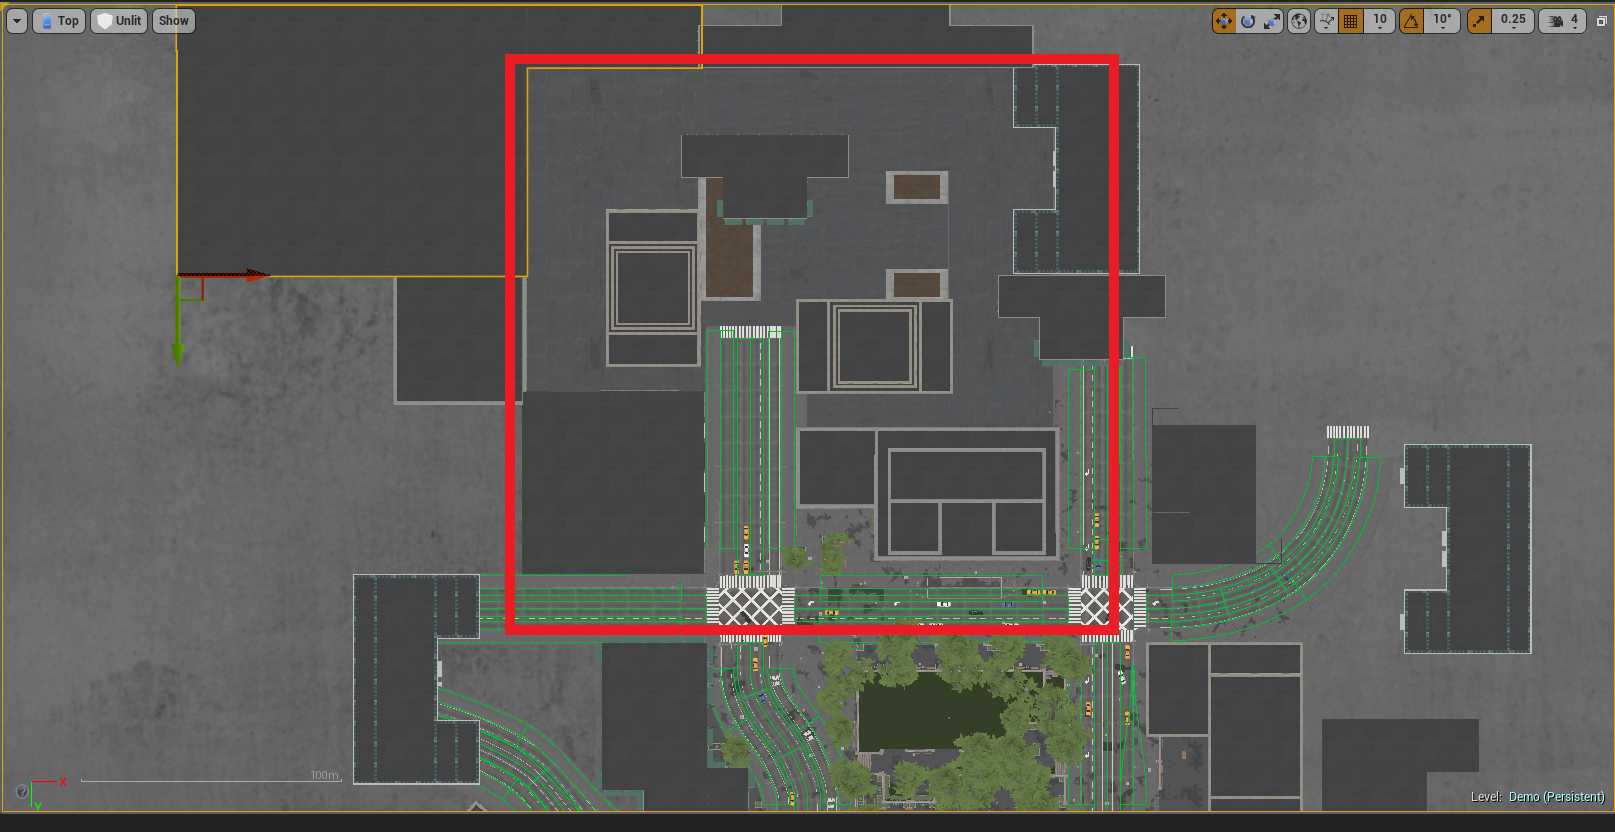
\includegraphics[width = 0.95\linewidth]{Surveillance/figs/downtown_map.png}}

\subfloat[The environment in \ref{fig:UE4city} is discretized into a 24x37 grid. Black cells are states that cannot be sensed from the current location of the agent. The agent is shown in blue, the evading target in orange. \label{fig:Airsim_grid}]{
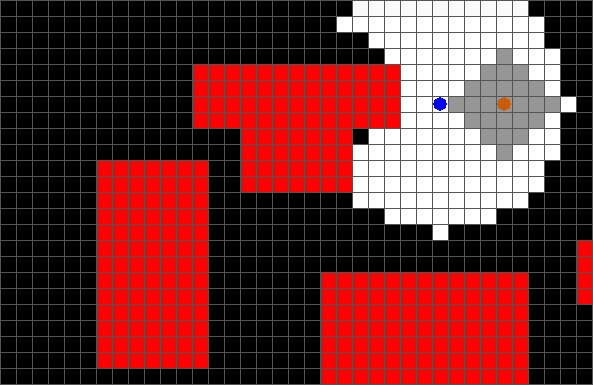
\includegraphics[width = 0.9\linewidth]{Surveillance/figs/Airsim_gridAirsim_Example.png}
}

\caption{The urban environment in Figure \ref{fig:GazArena} is discretized in \ref{fig:Airsim_grid} for synthesis. Note that due to the sensor uncertainty, the agent does not know the exact location of the target even when it is in range of its sensors.}
\label{fig:Airsim_casestudy}
\end{figure}
Figure~\ref{fig:Airsim_casestudy} depicts the top-down view environment created in \emph{Unreal Engine 4} and discretized for synthesis. The uncertainty in the sensing capaiblities of the agent is shown in Figure~\ref{fig:Airsim_grid} where grey cells correspond to the agent's current belief of the target's location stemming from the sensor and target state estimation uncertainty. The agent is 3 times faster than the target (it can move 3 cells for every 1 cell the target moves). 

In this setting, we require the satisfaction of the safety surveillance objective $\square p_{25}$ (the belief size should never exceed 25). In this case, we only need an abstraction with a trivial abstraction partition, consisting of the whole set of locations, as the agent has a strategy to closely follow and maintain view of the target. This is, in fact, necessary, as
any belief state will already be violating the safety requirement due to the estimation uncertainty. We are able to synthesize a strategy in 112 seconds. 
 
We present a video from the first-person view of the surveilling drone at \url{https://www.youtube.com/watch?v=HLsZ5ZnQgAg}. We note that the agent follows the target closely and never allows the target to leave its line of sight. In general, open urban environments the one considered here require stricter surveillance specifications as it is much harder to `find' a target once it has been lost. This will be in contrast with the more enclosed locations which we consider in the next case study.




\subsection{Liveness Surveillance Specification and Task Requirement} 
In this experiment, we demonstrate the behaviour an automatically synthesized strategy for the surveillance agent under a liveness surveillance specification and a task requirement. We do so in the Gazebo environment shown in Figure~\ref{fig:GazArena}. We compare this to a strategy for a safety surveillance specification with no additional task requirement, synthesized for the same environment. 



\begin{figure}
\subfloat[Lidar generated map of the gazebo environment in Figure~\ref{fig:GazArena}. \label{fig:Q_building_2}]{
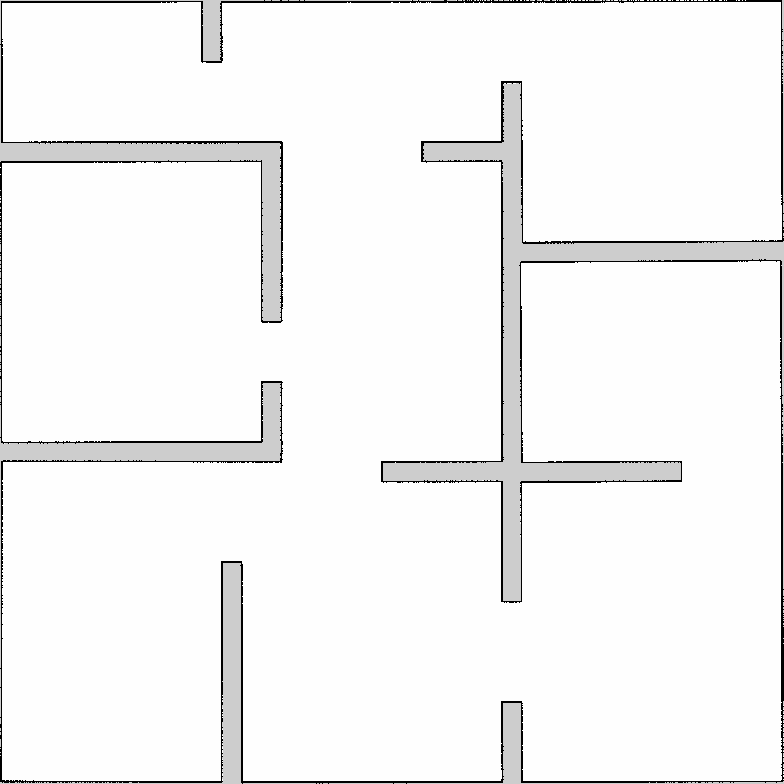
\includegraphics[width=0.45\linewidth]{Surveillance/figs/Q_building_2.png}
}
\hspace{0.5cm}
\subfloat[Discretization of the map \newline in Figure~\ref{fig:Q_building_2} used for synthesis \label{fig:gazebogrid}]{
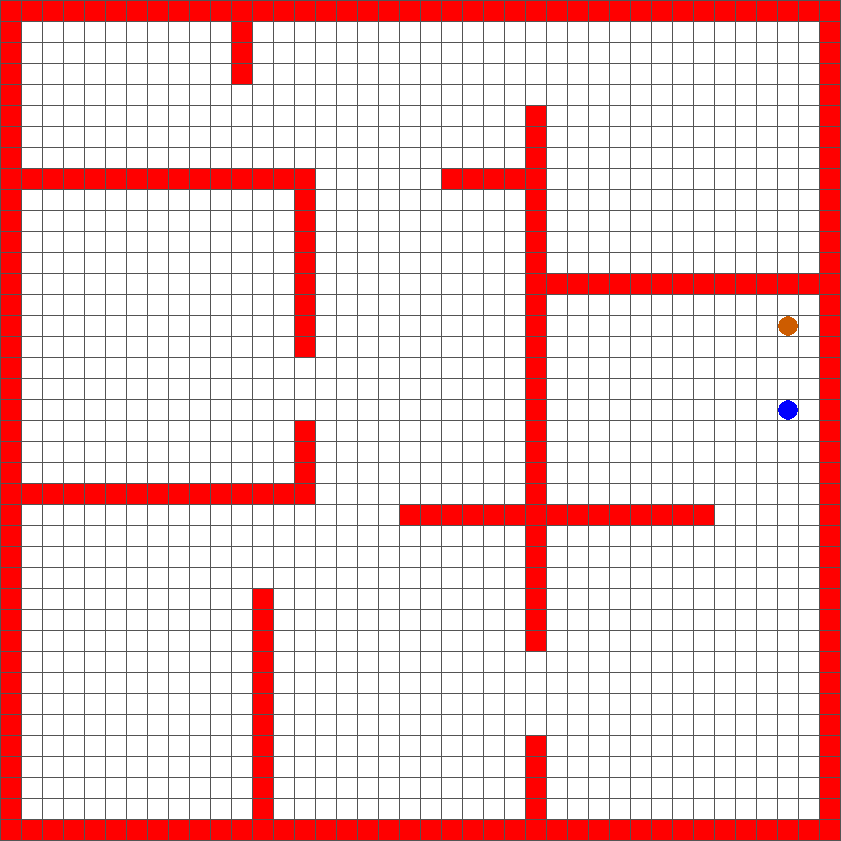
\includegraphics[width=0.45\linewidth]{Surveillance/figs/ROS_grid.png}\hspace{.5cm}
}

\caption{The Gazebo environment in Figure \ref{fig:GazArena} is first mapped using a LIDAR equipped agent to produce the map in~\ref{fig:Q_building_2} and then discretized to produce the gridworld in~\ref{fig:gazebogrid}.}
\label{fig:casestudiesros}

\end{figure}


The Iris quadcoptor shown in Figure~\ref{fig:sandiauav} is the agent being controlled by the synthesized surveillance strategy, and the Stanley Innovations Segway in Figure~\ref{fig:stanleyrobot} is the target. The target can either be controlled through a Python API or joystick such as an XBOX 360 controller. The quadcoptor uses a minimum snap trajectory package to plan its path, and a standard PX4 flight stack for the lower level flight control \cite{px4}. As in the previous section, we assume that the quadcoptor can move 3 times faster than the segway.

\begin{figure}[h]
  \definecolor{bg}{HTML}{ddeedd}
\definecolor{comp}{HTML}{c2d4dd}
\definecolor{impl}{HTML}{b0aac0}
\definecolor{ligb}{HTML}{5E7FC6}
\definecolor{bodybl}{HTML}{85A1DC}
\definecolor{headbl}{HTML}{264C9C}
\definecolor{bgyel}{HTML}{FFDC6B}
\definecolor{bodyyel}{HTML}{FFE58F}
\definecolor{headyel}{HTML}{E9BB25}
\definecolor{gr1}{HTML}{00FF00}
\definecolor{or1}{HTML}{FFAA00}
\definecolor{ye1}{HTML}{FFFF00}

% Define block styles
\tikzstyle{decision} = [diamond, draw, fill=blue!20, 
text width=4.5em, text badly centered, node distance=3cm, inner sep=0pt]
\tikzstyle{block} = [rectangle, draw, fill=blue!20, 
text width=5em, text centered, rounded corners, minimum height=4em]
\tikzstyle{line} = [draw, -latex']
\tikzstyle{cloud} = [draw, ellipse,fill=red!20, node distance=3cm,
minimum height=2em]
\def\checkmark{\tikz\fill[scale=0.6](0,.35) -- (.25,0) -- (1,.7) -- (.25,.15) -- cycle;} 
%
\centering
\begin{tikzpicture}[every node/.style={draw, text centered, shape=rectangle, rounded corners, text width=3cm, minimum height=0.8cm, inner sep=5pt}]
%\tikzstyle{outer}= [draw, text centered, shape=rectangle, text width=2cm, minimum height=1cm]
%\tikzstyle{inner}=[draw, text centered, shape=rectangle, rounded corners, text width=3.8cm, minimum height=1.1cm, inner sep=5pt]
\tikzstyle{decision} = [diamond, draw, aspect=3 , inner sep=3pt]


\node[fill=gr1!20!white] (launch){Launch};
\node[below=0.5cm of launch,fill=gr1!20!white] (move) {Flight};
\node[fill=blue!10!white,decision,below=0.5cm of move] (range) {Within range?};
\node[below=0.5cm of range,fill=or1!20!white] (loiter) {Loiter};
\node[fill=blue!10!white,decision,below=0.5cm of loiter] (assign) {Assigned?};
\node[below=0.5cm of assign,fill=ye1!20!white] (approach) {Approach};
\node[right=0.5cm of approach,fill=red!20!white,text width=1.5cm,inner sep=1pt] (land) {Land};

\path [line,-latex',very thick] (launch.south) -- (move.north);
\path [line,-latex',very thick] (move.south) -- (range.north);
\path [line,-latex', very thick] (range.south) --node[draw=none,right=-1.2cm]{Yes} (loiter.north);
\path [line,-latex', very thick] (range.east) -- node[draw=none,above=1pt] {No} ++(1.0,0)   |- (move.east);
\path [line,-latex', very thick] (loiter.south) --node[draw=none,left=-1cm]{Request} (assign.north);
\path [line,-latex', very thick] (assign.south) --node[draw=none,right=-1.2cm]{Land} (approach.north);
\path [line,-latex', very thick] (assign.east)  -- node[draw=none,above=1pt] {No} ++(1.0,0) |- (loiter.east);
\path [line,-latex', very thick] (assign.west)  -- node[draw=none,below=1pt] {Pass-through} ++(-1.0,0) |- (move.west);
\path [line,-latex', very thick] (approach.east) -- (land.west);


\end{tikzpicture}
    \caption{Flow chart of general procedure to synthesize surveillance strategies in Gazebo worlds and simulate the resulting strategies.}
    \label{fig:Flowmap}
\end{figure}


The Gazebo world is created using the building editor feature. An occupancy map of the world is created using the ROS Gmapping package. The Segway is manually driven around during mapping to generate the LIDAR map shown in Figure~\ref{fig:Q_building_2}. This map is then discretized to the map shown in Figure \ref{fig:gazebogrid} and used for the surveillance strategy synthesis. The output of the synthesis is a reactive controller which is stored as a look-up table for the quadcopter. %A summary of the implementation process is shown in Figure \ref{fig:Flowmap}.

 A ROS node first subscribes to a topic that is broadcasting the position of the segway, and converts that continuous position to the corresponding discrete location in the discretized gridworld. If the target cannot be sensed, then the state returned is a belief state. The synthesized strategy is then used by a ROS node to determine what waypoint the quadcopter should move to based on its current belief of the target's position. The action is converted to a continuous position to which the quadcoptor should move, a path from the current location to the new position is determined, and that complete path is sent to the PX4 controller which controls the quad along the path.

We synthesize two strategies in this environment under different surveillance specifications and qualitatively compare the different behaviours. First we consider the safety surveillance task $\LTLglobally p_1$. The quadcopter is never allowed to lose sight of the Segway. A human controls the segway with an XBOX controller and attempts to violate this specification and the resulting simulation can be seen at \url{https://www.youtube.com/watch?v=iFxmTUyVSoA}. Note that, just as in the previous section, the quadcopter follows the segway close enough to never lose sight of it, and the Segway is never able to hide. 


To contrast this behaviour, the quadcopter is next given the liveness surveillance task of $\LTLglobally \LTLfinally p_1$. Informally, the quadcopter has to infinitely often see the Segway directly, and is hence, allowed to lose sight of the Segway. Additionally the quadcopter has a task requirement of having to infinitely often return to a ``charging station" shown as a grey square in Figure~\ref{fig:GazArena}. The quadcopter can no longer simply closely follow the target as it must return to a different state infinitely often. Once again, a human controls the segway and attemps to hide. The corresponding simulation can be found at \url{https://www.youtube.com/watch?v=_l0h1m9q8F8}. 

% \todo{Explain (here and/or somewhere else) that repeated $\LTLglobally \LTLfinally p_1$  is not the same as repeatedly solving the simple reachability problem (pursuit-evasion game), as a strategy for simple reachability might lead to a state where the target us found but from then on has a strategy to evade forever.}

Due to the more enclosed  environment, the quadcopter can search the areas until it finds the segway. This allows for the satisfaction of additional task objectives. A joint liveness and task specification would often be unrealizable in environments similar to that in Figure~\ref{fig:Airsim_casestudy} as it is unlikely that the quad will be able to find the target if it loses sight of it for too long. 


The difference in the behaviour in the case studies highlights the different use cases of surveillance. Depending on the domain, the user can specify a combination of safety and liveness objectives, to tune the behaviour of the agent. In a critical surveillance situation (typical in defense or high-risk security situations), the safety specification will guarantee to the user that the belief will never grow too large. However, in less critical situations, the robot has more flexibility in allowing the belief to grow as long as it can guarantee its reduction in the future. Hence, a user can tune the desired qualitative behavior depending on their specific use case. 

% The Unreal Engine 4 editor was used to create the jungle environment. The Airsim plugin is used to simulate and control the vehicles. ---- Not sure what else to put. Will depend on if we use a jungle environment in a sim. ----

% Next the set of discretized states are bundled manually into belief partitions. Then the SLUGS input file is constructed with a script from the surveillance objectives, vehicle parameters, the belief partition sets, and the discretization of the Gazebo world. SLUGS outputs a reactive controller as a JSON file.

% The vision dictionary and the controller generated by SLUGS are used by a ROS node to determine if the target can be seen and what action the agent should take.The state of the agent and target are used to look up what action the agent should take. 
%
%%%%%%%%%%%%%%%%%%%%%%%%%%%%%%%%%%%%%%%%%%%%%%%%%%%%%%%%%%%%%%%%%%%%%%%%%%%%%%%%%
%
%\section{CONCLUSIONS}
%%We have provided a systematic, and general, approach to solving surveillance problems for autonomous agents. The framework we present extends previous work by including additional sensor modalities such as static sensors and accounting for imperfect sensors. Furthermore, we show the viability of the framework by simulating the execution of the synthesized surveillance strategies in realistic simulation environments against human controlled adversaries. Some directions of future work that we are currently exploring include the following:
%
%\begin{itemize}
%
%\item allowing for false positives to occur in target state estimation;
%\item automated generation of the initial abstraction based on features of the map of the surveillance area;
%    \item implementation and execution of the synthesized surveillance strategies on actual hardware;
%    \item considering different classes of targets, for example, both hostile and non-hostile targets;
%    \item learning the behaviour of a target over time, to allow the agent to improve its performance while still guaranteeing the satisfaction of the surveillance specification. 
%\end{itemize}



We have presented a novel approach to solving a surveillance problem with information guarantees. We provided a framework that enables the  formalization of the surveillance synthesis problem as a two-player, partial-information game. We then presented a method to reason over the belief that the agent has over the target's location and specify formal surveillance requirements. The user can tailor the behaviour to their specific application by using a combination of safety and liveness surveillance objectives. Furthermore, we show the viability of the framework by simulating the execution of the synthesized surveillance strategies in realistic simulation environments as well as on hardware against human controlled adversaries.

The benefit of the proposed framework is that it allows it leverages techniques successfully used in verification and reactive synthesis to develop efficient methods for solving the surveillance problem. There are several promising  avenues of future work using and extending this framework. Some of which currently being explored are the following;
\begin{itemize}

\item allowing for false positives to occur in target state estimation;
\item automated generation of the initial abstraction based on features of the map of the surveillance area;
    \item considering different classes of targets, for example, both hostile and non-hostile targets;
    \item learning the behaviour of a target over time, to allow the agent to improve its performance while still guaranteeing the satisfaction of the surveillance specification. 
\end{itemize}

%%%%%%%%%%%%%%%%%%%%%%%%%%%%%%%%%%%%%%%%%%%%%%%%%%%%%%%%%%%%%%%%%%%%%%%%%%%%%%%%


%%%%%%%%%%%%%%%%%%%%%%%%%%%%%%%%%%%%%%%%%%%%%%%%%%%%%%%%%%%%%%%%%%%%%%%%%%%%%%%%

\chapter{Surveillance}

%A framework is needed in which humans can easily specify desirable high-level qualitative behaviour for autonomous systems performing complex tasks.
In this chapter, we investigate these questions in the context of autonomous agents that perform \emph{surveillance} tasks, that is, tracking the location of a target. 


Performing autonomous surveillance has many applications. If the target is adversarial, these applications include patrolling and security, especially in combination with other objectives, such as providing certain services or accomplishing a mission. For example, unmanned aerial vehicles (UAVs) are increasingly being adopted for monitoring of illegal hunting and poaching \cite{poaching}. In countries such as Kenya, South Africa, and Zimbabwe \cite{drones}, drones have been deployed and tested in an attempt to reduce poaching by providing continuous surveillance \cite{poaching}. However, all of these solutions still require a pilot to remotely operate the UAV or manually provide it with waypoints to follow. Autonomous surveillance has the potential to help combat poaching by drastically reducing manpower requirements. 

Autonomous surveillance also has many applications where the targets are not adversarial, but are unpredictable. One such example involves mobile luggage carrying robots in airports that are required to follow a human despite unpredictable motion and possibly sporadically losing sight of the target \cite{GonBanos02}. 

When dealing with an adversarial and/or unpredictable moving target, a strategy for the surveying agent to achieve its objective can be seen as a strategy in a two-player game between the agent and the target. Since the agent may not always observe, or even know, the exact location of the target, surveillance is, by its very nature, a partial-information problem.
It is thus natural to reduce surveillance strategy synthesis to computing a winning strategy for the agent in a two-player partial-information game. Game-based models for related problems have been extensively studied in the literature. Notable examples include pursuit-evasion games~\cite{Chung2011}, patrolling games~\cite{Basilico12}, and graph-searching games~\cite{Kreutzer11}, where the problem is formulated as enforcing eventual detection, which is, in its essence a search problem -- once the target is detected, the game ends. For many applications, this formulation is too restrictive. Often, the goal is not to detect or capture the target, but to maintain certain level of knowledge about its location over an unbounded time duration, or, alternatively, be able to obtain sufficiently precise information over and over again. In other cases, the agent may have an additional objective, such as performing a certain task, which might prevent it from capturing the target, but allow for satisfying a more relaxed surveillance objective.

In this paper, we study the problem of synthesizing strategies for enforcing \emph{quantitative temporal surveillance objectives}, such as the requirement to never let the agent's uncertainty about the target's location exceed a given threshold, or recapturing the target every time it escapes. To this end, we consider surveillance objectives specified in linear temporal logic (LTL), equipped with basic surveillance predicates. This formulation also allows for a seamless combination with other task specifications.

We model the problem as a two-player game played on a finite graph, whose nodes represent the possible locations of the agent and the target, and whose edges model the possible (deterministic) moves between locations. The agent plays the game with partial information, as it can only observe the target when  it is in range of its sensors. The target, on the other hand, always has full information about the agent's location, even when the agent is not in sight. In that way, we consider a game with one-sided partial information, making the computed strategy for the agent robust against a potentially more powerful adversary. \looseness=-1

%We formulate surveillance strategy synthesis as the problem of computing a winning strategy for the agent in a partial-information game with a surveillance objective. 
There is a rich theory on partial-information games with LTL objectives~\cite{DoyenR11,Chatterjee2013}, and it is well known that, in general, the synthesis problem is EXPTIME-hard~\cite{Reif84,BerwangerD08}. Moreover, all the standard algorithmic solutions to the problem are based on some form of \emph{belief-set construction}, which transforms the \emph{imperfect}-information game into a \emph{perfect}-information game. However, the new set of states in the perfect-information game is the powerset of the original state space in the imperfect-information game. Thus, such approaches scale poorly in general, and are not applicable in most practical situations.

We address the state-space explosion problem from the belief-set construction by using \emph{abstraction}. We introduce an \emph{abstract belief-set construction}, which under-approximates the information-tracking abilities of the agent (or, alternatively, over-approximates its belief, i.e., the set of positions it knows the target could be in). Using this construction we reduce surveillance synthesis to a two-player perfect-information game with an LTL objective, which we then solve using off-the shelf reactive synthesis tools~\cite{EhlersR16}. The abstract belief-set construction guarantees that the abstraction is sound, that is, if a surveillance strategy is found in the abstract game, it corresponds to a surveillance strategy for the original game. If, on the other hand, such a strategy is not found, then the method automatically checks if this is due to the coarseness of the abstraction, in which case the abstract belief space is automatically refined. Thus, the method follows the general counterexample-guided abstraction refinement (CEGAR)~\cite{ClarkeGJLV00} scheme, which has successfully demonstrated its potential in formal verification and synthesis.

{\bf Contributions.}  This paper makes the following contributions:\\
(1) We present a novel framework for encoding \emph{quantitative surveillance} and other task requirements against adversarial agents and synthesising strategies that satisfy the given requirements.\\
(2) This framework is capable of handling \emph{uncertainty in sensor outputs} as well as \emph{multiple sensor modalities}, and it can hence incorporate realistic scenarios from surveillance applications.  \\
(3) We design a belief abstraction approach to solve the partial-information game and develop an algorithm that \emph{automatically refines a given abstraction} in order to improve its precision when no surveillance strategy exists due to coarseness of the approximation.\\
(4) We implement and execute the synthesized surveillance strategies in multiple \emph{high-fidelity simulation} environments and thus demonstrate the adaptability and practical viability of the approach in realistic robotics applications.



{\bf Related work.}
While closely related to the surveillance problem we consider, pursuit-evasion games with partial information~\cite{Chung2011, Chin2010, Antoniades2003} formulate the problem as eventual detection, and do not consider combinations with other mission specifications. Other work, such as \cite{Vidal2002} and \cite{Kim2001}, additionally incorporates map building during pursuit in an unknown environment, but again solely for target detection.

Synthesis from LTL specifications~\cite{Pnueli1989}, especially from formulae in the efficient GR(1) fragment~\cite{Piterman2006}, has been extensively used in robotic planning (e.g.~\cite{wong2012,Kress2007}), but surveillance-type objectives, such as the ones we study here, have not been considered so far. Epistemic logic specifications~\cite{MeydenV98} can model the knowledge of the agent on the truth-value of logical formulas, however, contrary to the surveillance specifications in this paper, they are not capable of expressing requirements on the size of the agent's uncertainty.

CEGAR has been developed for verification~\cite{ClarkeGJLV00}, and later for control~\cite{HenzingerJM03}, of LTL specifications. 
It has also been extended to infinite-state partial-information games~\cite{DimitrovaF08}, and used for sensor design~\cite{FuDT14}, both in the context of safety specifications. In addition to being focused on safety objectives, the refinement method in~\cite{DimitrovaF08} is designed to provide the agent with just enough information to achieve safety, and is thus not applicable to surveillance properties whose satisfaction depends on the size of the belief sets.

This paper generalizes the method presented in~\cite{bharadwaj2018synthesis} and ~\cite{bharadwaj2018distributed} to allow for uncertainty in sensor measurements and multiple sensor modalities. More precisely, we consider sensors that return sets of possible values (for example the set of possible positions of the target whose likelihood is above some given threshold), and include static sensors in addition to the mobile agent. Additionally, we present an automated counterexample-guided abstraction refinement algorithm, while previous work relied solely on user-provided abstractions. Finally, this paper presents simulations on ROS/Gazebo, and Unreal Engine 4 with agents reacting in real-time to a human-controlled adversary.

The rest of the paper is structured as follows. In section II we present a case study to motivate the work in this paper in the context of a real-world security application. In section III we provide definitions and notations for partial-observation games and the encoding of the surveillance requirement as safety and liveness objectives in LTL. In section IV, we present the belief set abstraction in reducing the partial information game to a full information game. In sections V and VI we detail the CEGAR process for the different types of surveillance objectives. In section VII, we demonstrate the framework on gridworld examples to illustrate how abstract belief states are constructed and refined. In section VIII, we implement the surveillance strategy synthesis procedure using Gazebo/ROS as well as unreal engine on robot platforms with simulated LiDAR sensors. Lastly, we conclude and outline future directions in section IX.  



%Performing surveillance on an adversarial target, by its very nature, is a partial information problem. The agent may not always know the position of the target. However, surveillance in conjunction with a mission specification can be crucial in applications such as defense where it is important to keep track of (potentially hostile) targets whilst trying to satisfy a particular objective. 

%Since we are dealing with an adversarial target, a natural setting for formulating the problem is a two-player game. There are several flavours of partial information games that have been studied in the literature \cite{Chatterjee2013}, and in this paper we focus on turn-based one-sided partial-observation deterministic games on which we perform reactive control synthesis. It is one-sided as we allow the adversary full information on the location of the agent even if it is not in sight. 

%Related work in dealing with surveillance type objectives are pursuit-evasion games. There are several methods in formulating the problem such as enforcing eventual detection (at which point the game ends) \cite{Chen2010} or not allowing the target to move more than a certain distance away (\cite{keylist}). Partial information version of these games have also been studied in \cite{Antoniades2003,keylist} where it is shown that there is no existence theory for optimal solutions. However, these approaches treat the surveillance requirement as a search problem - once the target is detected the game is over. Work done by \cite{Vidal2002} and \cite{Kim2001} also include map building during pursuit but again with the sole purpose of target detection. Additionally, we do not enforce the requirement that the target(s) be detected. It is sufficient if we are able to bound our belief of the location below a user specified threshold for an infinite execution which allows for more richer, and more complex, behaviour than standard pursuit-evasion. So while there is work in pursuit-evasion games with partial information \cite{Chen2010} and even unknown environments \cite{Vidal2002}, these do not deal with additional mission specifications and also do not allow for the target to 'escape' and be recaptured as will be necessary in a setting with objectives beyond only capture.

%Our aim is to then synthesize a reactive controller that satisfies both the LTL specification as well as the surveillance objective. While it has been shown that for a general LTL specification, the synthesis problem is doubly exponential in the length of the formula \cite{Pnueli1989}, the work in \cite{Piterman2006} lays out a class of formulae called GR(1) that is $\mathcal{O}(N^3)$. This framework has been used extensively in robotic planning, for example in \cite{wong2012,Kress2007} and we do so here as well. We explicitly encode the surveillance requirement into the GR(1) formula to allow us to exploit the fast nature of GR(1) synthesis to solve a pursuit-evasion game. 

%However, we still have the issue of partial obsno ervability in our setting. The controller will need to choose actions even when the state of the adversary is not known. The standard approach to deal with the partial observability is by using a \emph{belief set construction} to reduce the problem to a full observability game \cite{Bertoli2006}. However, the number of belief states will be exponential in the number of states \cite{Rintanen2004} as the belief set construction takes a powerset of the number of states. In general, this scales poorly and is not usable in most practical situations. \todo{literature on other partial information reduction heuristics}. In this paper, to deal with this problem, we introduce \emph{abstract belief set construction}. This is an underapproximation of the true belief space and hence, if a controller is found, then we know a controller will exist in the fully refined belief space. If a controller is not found, we use counterexample guided abstract refinement (CEGAR) to split a belief set and the process is repeated. While CEGAR has been extensively used on abstract models for GR(1) reactive synthesis \cite{Alur2015,keylist}, to our knowledge it has not been used on belief state refinement in reducing a partial information game to a full information game. 

%The focus of this paper is to solve a modified pursuit-evasion game with additional LTL objectives in a partial information setting using reactive control synthesis. We propose a novel encoding of the surveillance requirement into the GR(1) specification to allow for assume guarantee control synthesis as well as a CEGAR approach in belief set construction in solving the partial information game. Our contributions in this paper are as follows:
%\begin{itemize}
%\item We encode the surveillance task as a safety specification which forces the agent to more closely follow the adversary in order to ensure the uncertainty (size of the belief set) on the location of adversary does not grow above the constraint.
%\item We also encode surveillance task as a liveness objective. This allows for the agent to be more relaxed in monitoring the location of the agent if it can ensure that it can see it again sometime in the future.
%\item We analyse the qualitatively different behaviour produced based on the specification type which allows the user to tailor the specification based on the requirements of the mission.
%\item Avoiding the state space blow up by abstract belief set construction and using counter example guided belief refinement for both the safety and liveness specification cases.
%\end{itemize}

%The rest of the paper is structured as follows. In section II we provide definitions and notations for partial-observation games and the encoding of the pursuit-evasion requirement as safety and liveness objectives in LTL. In section III, we present our belief set abstraction in reducing the partial information game to a full information and also detail the CEGAR process for the different types of objectives. In section IV we provide experiments on gridworlds along with a simulation in ROS using our proposed algorithm, and we conclude and provide future direction in section V. 



%%%%%%%%%%%%%%%%%%%%%%%%%%%%%%%%%%%%%%%%%%%%%%%%%%%%%%%%%%%%%%%%%%%%%%%%%%%%%%%%

% \section{Motivating Scenario}
% In this section, we demonstrate the effectiveness of the proposed framework to a case study for an urban security application with high-fidelity simulated sensors and robots. 
%Physical security applications typically require the housing and protection of sensitive materials or locations. Often, such environments are large and it is difficult to have complete surveillance coverage at all times using only static sensors. In such situations, deploying an autonomous mobile agent with sensing capabilities can greatly reduce coverage requirements from static sensors. When utilizing autonomous agents it is necessary to provide quantitative guarantees on their belief of the location of an intruding target in order to direct security measures accurately. The method proposed in this paper generates strategies for fully autonomous surveillance with quantitative guarantees on the size of the belief of the target's location and hence is a natural fit for security applications. 
We provide the code for the implementation on Github\footnote{Github: \url{https://github.com/u-t-autonomous/Surveillance}} and the videos for all simulations at the corresponding Github page \footnote{Github page: \url{https://u-t-autonomous.github.io/Surveillance-Synthesis/}}.
%We will use the case study to demonstrate the versatility and applicability of our surveillance strategy and belief abstraction methods across multiple high-fidelity simulation environments.

% \subsection{Combating poaching}
% First, consider the problem of tracking poachers in Africa. 
% UAVs are increasingly being adopted for monitoring of illegal hunting and poaching \cite{poaching}. In countries such as Kenya \cite{poaching}, South Africa, and Zimbabwe \cite{drones}, drones have been deployed and tested in an attempt to reduce poaching by providing constant surveillance \cite{poaching}. However, all of these solutions still require a pilot to remotely operate the UAV or manually provide it waypoints. In this paper we propose a method to generate strategies that can allow for \emph{fully autonomous surveillance} with quantitative guarantees on the \emph{belief in the position of the target}. These quantitative guarantees allow a response to be effectively mobilized by relevant authorities. 

% We simulate a jungle environment using Unreal Engine 4 as shown in Figure \ref{fig:UE4JungleProto} and UAVs are simulated in the environment using an Airsim plugin \cite{airsim}. In Section VII we present simulations of an autonomous UAV performing surveillance mission in this environment. 

% \begin{figure}[h]
%     \centering
%     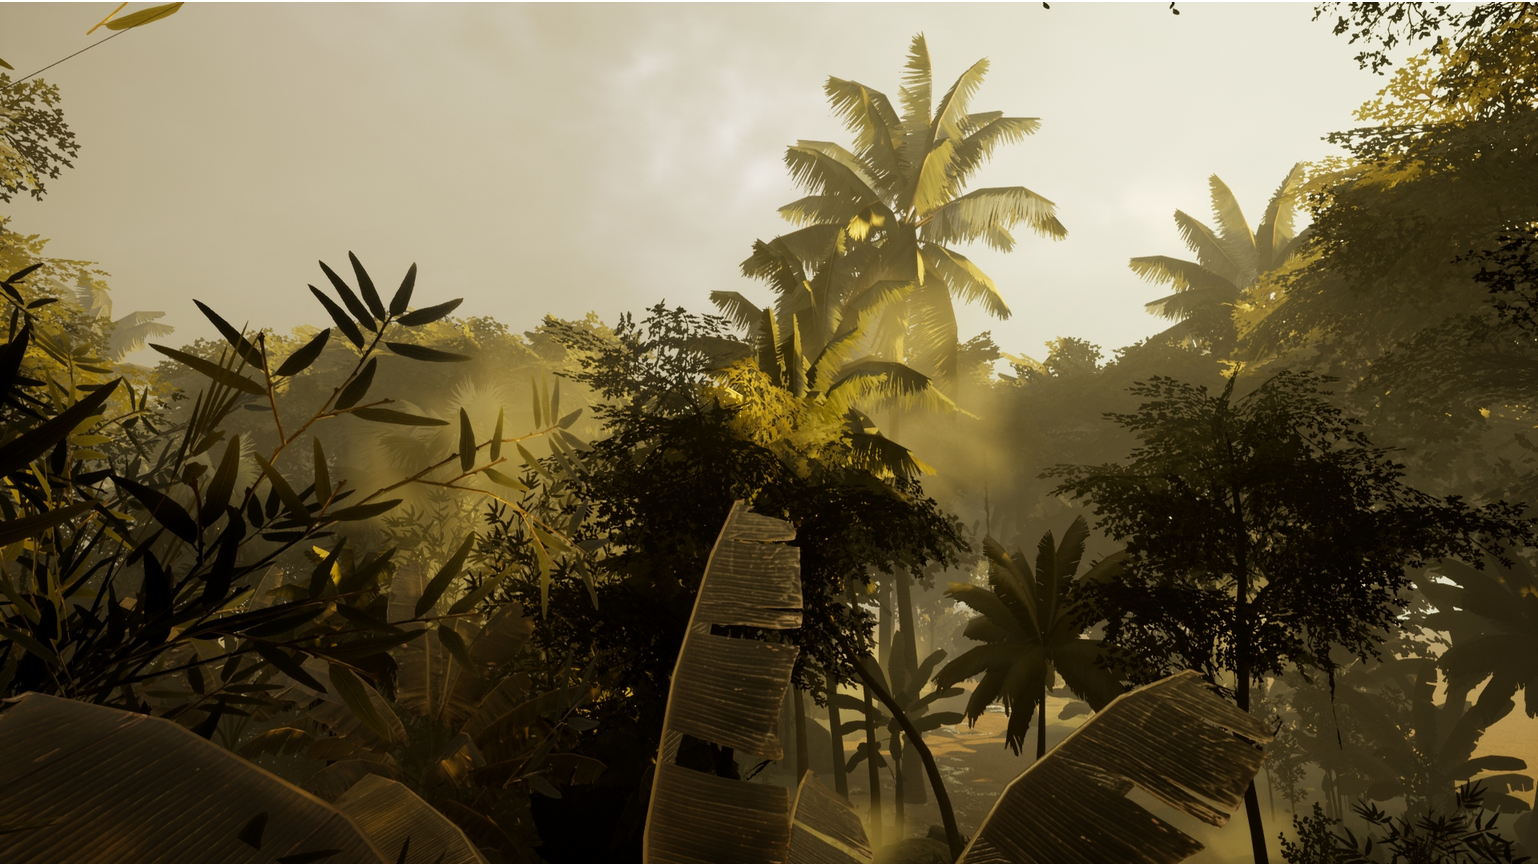
\includegraphics[width = 0.9\linewidth]{figs/UE4JungleProto.png}
%     \caption{Unreal Engine 4 Jungle Environment}
%     \label{fig:UE4JungleProto}
% \end{figure}
%\subsection{Security}



% \begin{figure}[h]
%     \centering
%     \includegraphics[width = 3 in]{figs/GazArena.png}
%     \caption{Gazebo Environment}
%     \label{fig:GazArena}
% \end{figure}

%andia National Labs considers examples where there is a compound that has a sensitive area that must be protected and is surrounded by land that contains wild life. Sometimes when an intruder is detected, the security system cannot determine if the threat is real or if there is simply an animal wandering around. A security officer must then go out and find the intruder to determine the state of the threat. In order to reduce wasted time, actively tracking that threat to provide the security personnel with a small region to search instead of a last known location saves resources. 

%and of security around a sensitive compound where tracking potential intruders is required for security personnel to make contact with and determine if the threat is real or false.




\subsection{Robot Platforms}

We use two robot simulation platforms to demonstrate the generality and applicability of the platform-agnostic methodology developed in this paper:
\begin{enumerate}
    \item An Iris quadcopter, which uses the PX4 flight stack and is capable of waypoint control.
    \item Stanley Innovations segway, which uses the ROS navigation stack for mapping, waypoint control, and autonomous obstacle avoidance. 
\end{enumerate}
To simulate the sensor output, we directly access the ground truth position of the moving target and add noise. We model the sensor and state estimation uncertainty as described in section \ref{sec:sensefunction} using a simulated 360 degree LiDAR with range of  $10$ meters, angular resolution of 1 degree, range accuracy of $\pm 3$ cm.


The function $vis$ is built directly from the sensor range parameter. To construct the function $sense$ we use a worst-case conservative Gaussian noise model. Given a sensor measurement, let $0 \leq p(l) \leq 1$ be the probability the target is in location $l$. We construct the uncertainty set $U$ of possible target states for each sensor measurement $sense(l_a,l_t)$ by including all states with a probability greater than $\delta$ where $0\leq \delta \leq 1$ can be set by the user. In the following simulations, we use $\delta = 0.95$. Informally, if a target is in sensor range, the agent's belief consists of \emph{all states} at which the target is with a probability greater than or equal to $5\%$. We note that, since the function $obs$ depends only on the sensors, the function needs to be constructed only once and can be used for all robots that use the same sensors. 
We test the synthesized surveillance strategies synthesized in two environments. One is an open urban-like setting modelled in Unreal Engine 4 depicted in Figure \ref{fig:UE4city}. A quadcopter acts as the surveilling agent and another acts as a potential intruder. In the second scenario, we consider an enclosed compound-like environment modelled in Gazebo as shown in Figure \ref{fig:GazArena}. The Iris quadcopter is tasked with tracking a hostile target (the Stanley Innovations segway) and maintaining sufficient knowledge of its location. We allow a human to directly control the rover and demonstrate the corresponding real-time response of the quadcopter to satisfy its surveillance task. We also perform the same experiment with the quadcopter controlled by a human and the Segway as the autonomous surveilling agent to emphasise that the framework is agnostic to the specific underlying hardware and can be easily applied. 
  
We contrast the surveillance needs and the qualitatively different resulting behaviours of the synthesized strategies for the agents in these two environments.

\begin{figure}
\centering


\subfloat[Urban environment modeled in Unreal Engine 4 \label{fig:UE4city}]{
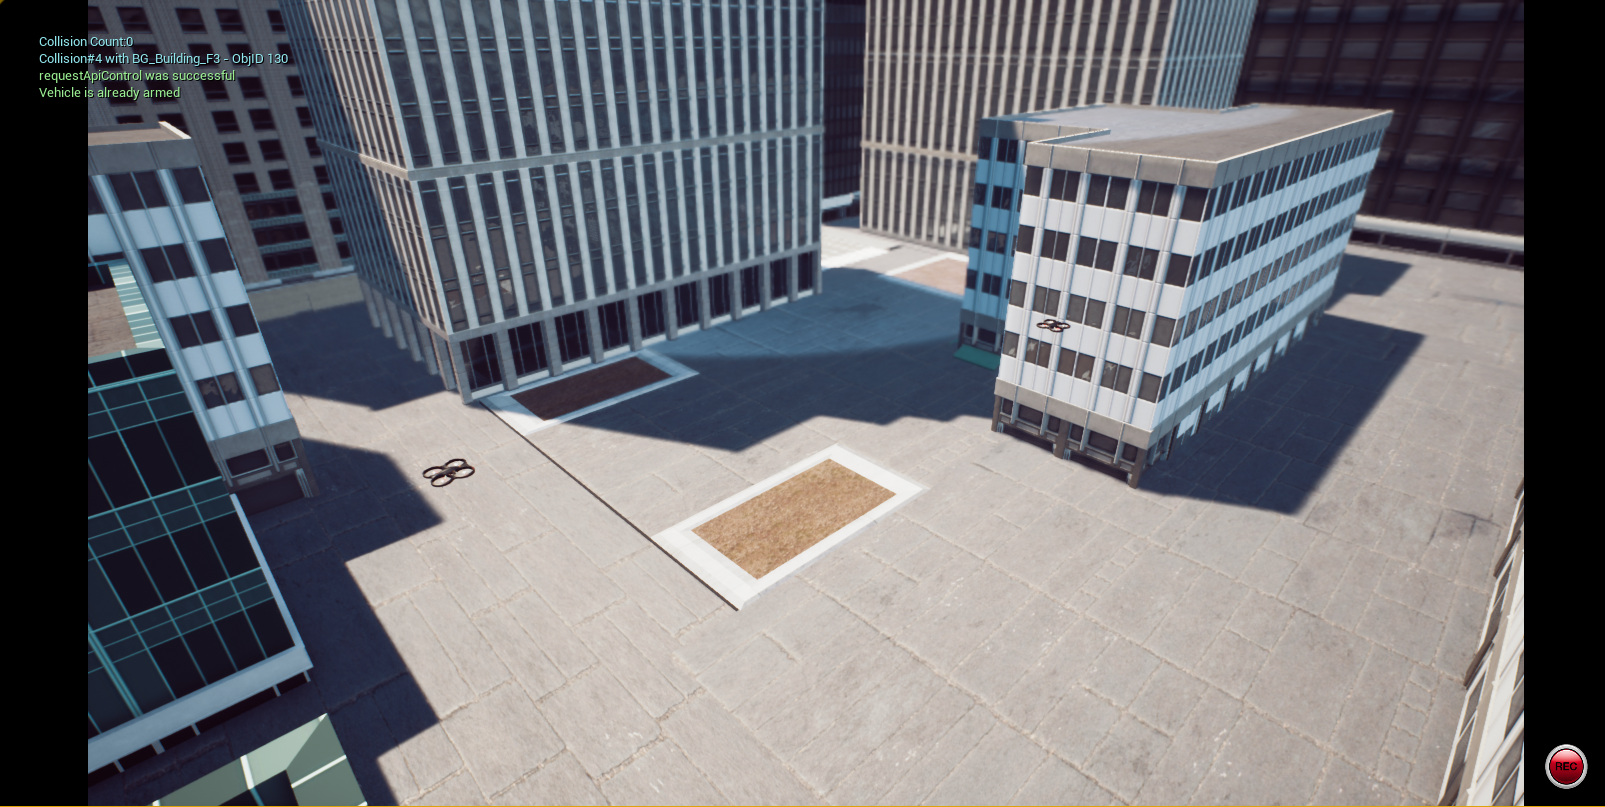
\includegraphics[width = 0.9\linewidth]{Surveillance/figs/unreal_city.png}}

\subfloat[Enclosed compound modelled in Gazebo \label{fig:GazArena}]{
\includegraphics[width = 0.9\linewidth]{Surveillance/figs/GazArena.png}}

\subfloat[Iris quadcopter used for autonomous surveillance \label{fig:sandiauav}]{
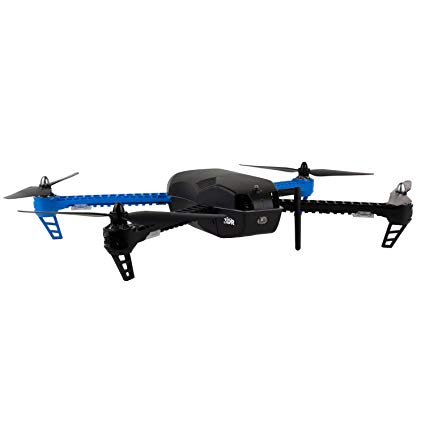
\includegraphics[width = 0.43\linewidth]{Surveillance/figs/quad.jpg}
} \hspace{0.05\linewidth}
\subfloat[Stanley innovations segway vehicle acting as a hostile target \label{fig:stanleyrobot}]{
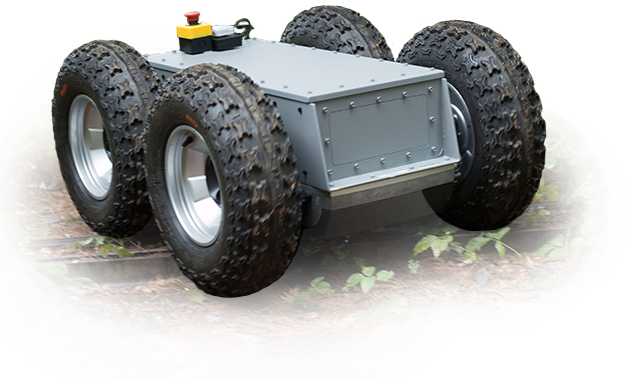
\includegraphics[width = 0.43\linewidth]{Surveillance/figs/Rugged-All-Terrain.png}
}

\caption{Case study for a security application. The vehicles are simulated in either Gazebo environment shown in \ref{fig:GazArena} or a UE4 environment shown in \ref{fig:GazArena}. A user can act as an `intruder' by controlling a target \ref{fig:stanleyrobot}. The UAV in \ref{fig:sandiauav} must autonomously react to guarantee the surveillance mission is satisfied. }
\label{fig:SandiaCaseSTudy}
\end{figure}

%%%%%%%%%%%%%%%%%%%%%%%%%%%%%%%%%%%%%%%%%%%%%%%%%%%%%%%%%%%%%%%%%%%%%%%%%%%%%%%%

\section{GAMES WITH SURVEILLANCE OBJECTIVES}\label{sec:gamedef}
%\subsection{Overview}\label{sec:problemoverview}
 Consider an environment consisting of an operating space and a network formed from a series of $k$ UAM vertiport hubs labeled $V_1,\cdots,V_k$. A UAM vertiport hub (henceforth referred to as a vertihub) consists of a grouping of multiple vertiports, each of which may have multiple takeoff/landing pads. A vertihub is responsible for managing requests by UAM vehicles (henceforth referred to as vehicles) to either \emph{land at} or \emph{take off from} a desired vertiport in its region or \emph{pass through} to a neighboring region. Each vertiport inside a vertihub is in charge of taking off and landing vehicles at its landing pads. An example of such an environment is illustrated in Figure~\ref{fig:RegionsOutline}. Note that vertihub control regions need not be circular. 
\begin{example}
The vertihub controller for region $V_6$ in Figure~\ref{fig:RegionsOutline} controls the operational area defined by $V_6 - (V_6 \cap V_5)$. The area of overlap $H_{56} = V_5 \cap V_6$ is the region where the handoff takes place, wherein the vertihub controller of the region the vehicle is about to enter takes responsibility for the vehicle.
Hence, $V_6$ can force vehicles incoming from $V_5$ to loiter in the handoff region $H_{56}$ until it is safe to allow them to enter.
\end{example}

The number of vehicles allowed inside each vertihub is upper bounded both by the separation standards between the vehicles as well as with the complexity of the airspace (e.g., intersection with general aviation traffic etc.).
Vertihubs cannot accept vehicles (i.e., accept a handoff) if the additional vehicle exceeds the maximum operational capacity or induces a conflict. Furthermore, vertiports cannot allow vehicles to take-off if it will violate the maximum operational capacity of the vertihub, and must force incoming vehicles to loiter if all of their pads are occupied. In order to avoid violating airspace requirements and to avoid build up of loitering vehicles (which can delay vehicles desiring to pass through or create safety issues), a vertiport must coordinate with its corresponding vertihub. We model the vertihub controller and vertiport controllers as \emph{reactive systems}.
%The hub can then act tactically by blocking a vehicle's entry to the region by making it loiter in a \emph{handoff region}.

\paragraph*{\textbf{Definition}}
We consider a finite set $\inp$ ($\out$) of Boolean \emph{inputs (outputs)}.
The input alphabet is
$\ialphabet=2^\inp$, the output alphabet is $\oalphabet=2^O$, and
$\alphabet=\ialphabet \times \oalphabet$. The set of finite (infinite) traces
over $\alphabet$ is denoted by $\alphabet^*$ ($\alphabet^\omega$), and
we define $\alphabet^{\infty} = \alphabet^* \cup \alphabet^\omega$.  A reactive system is a
tuple $\design = (\states,q_{0},\ialphabet,\oalphabet,\delta,\lambda)$,
where
$\states$ is a finite set of states,
$q_{0} \in \states$ is the initial state,
$\ialphabet$ is the input alphabet,
$\oalphabet$ is the output alphabet,
$\delta: \states \times \Sigma_{\inp} \to \states$ is the complete transition function, and $\lambda : \states \times \Sigma_{\inp} \to \Sigma_{\out}$ is the output function.
%
Given an input trace $\itrace = x_0 x_1 \ldots \in \ialphabet^\infty$, a reactive system $\mathcal{\design}$ produces an
output trace $\otrace = \mathcal{\design}(\itrace) = \lambda(q_0, x_0)
\lambda(q_1, x_1) \ldots \in \oalphabet^\infty$ with $q_{i+1} = \delta(q_i, x_i)$ for all $i \ge 0$.
The set of words produced by
$\mathcal{\design}$ is denoted $\lang(\mathcal{\design}) = \{\itrace \parallel \otrace \in
\alphabet^\infty \mid \mathcal{\design}(\itrace) = \otrace\}$.



\begin{figure}[h!]
	\centering

\newcommand{\OperatorSpace}[5]{
				%\draw[rounded corners = 15pt,dashed] (#1-#4,#2-#5) rectangle (#1+#4,#2+#5);
		\fill[fill=green,opacity=0.2] (#1,#2) circle (#3);
		\draw[draw = black,dashed](#1,#2) circle (#3);
		%\node at (#1,#2-#5+0.5) {$V_{#6}$};
	}

	

		\subfloat[ Example UAM operating environment \label{fig:RegionsOutline}]{
		\scalebox{1.75}{
		\begin{tikzpicture}[scale=0.3]
			\OperatorSpace{0}{0}{3}{5}{5}
			%\node at (-4.25,4.25){$S_1$};
			\node at (-1.5,1.5){$V_1$};
			\OperatorSpace{3}{-4}{3}{5}{5}
			%\node at (-1.25,-8.25){$S_2$};
			\node at (2.5,-4.5){$V_2$};
			\node[red] at (2.5,3) (H13) {$H_{13}$};
			\draw [->,red,line width = 0.75mm] (H13) -- (2.5,1.25);
			\OperatorSpace{5}{0}{3}{5}{6}
			%\node at (5-4.25,5.5){$S_3$};
			\node at (5-0.5,2){$V_3$};
			\node[red] at (6.5,3.5) (H35) {$H_{35}$};
			\draw [->,red,line width = 0.75mm] (H35) -- (6.75,0.65);
			\OperatorSpace{10}{0}{4}{6}{7}
			
			\node at (8.5-0.5,-5.5){$V_4$};
% 			\node[red] at (6.5,3.5) (H35) {$H_{35}$};
			\draw [->,red,line width = 0.75mm] (H35) -- (6.75,0.65);
			\OperatorSpace{6.5}{-4}{2.5}{0}{0}
			
			%\node at (10+5.25,-6.5){$S_5$};
			\node at (10+1.5,-1.5){$V_5$};
			\OperatorSpace{15}{2}{3}{5}{5}
			\fill[blue] (-1.5,-1.5) rectangle (-1,-1);
			%\node at (15-4.25,5+3.25){$S_6$};
			\node at (15,3.5){$V_6$};
			\node[red] at (11,4.5) (H56) {$H_{56}$};
			\draw [->,red,line width = 0.75mm] (H56) -- (12.5,2.75);
			\draw (17,3) node[cross,blue]{};
			\draw[blue,line width = 0.5mm] plot [smooth,tension=1] coordinates{(-1.5,-1.5) (3,0.5) (10,0) (17,3)};
			\draw (-0.5,2) node[cross,black]{};
			\fill[black] (7.5,-5.5) rectangle (7.0,-5.0);
			\draw[black,line width = 0.5mm] plot [smooth,tension=1] coordinates{(-0.5,2) (3,-0.5) (7,-5.0)};
			
		\end{tikzpicture}}}\\
\subfloat[Connectivity graph \label{fig:Environment_directed}]{
\scalebox{1.25}{
\begin{tikzpicture}[auto,node distance=8mm,>=latex,font=\small]
        \tikzstyle{round} = [thick,draw=black,circle]
\tikzstyle{action} = [circle, draw, fill=black,inner sep=0pt, minimum size=4pt]
\node[round] (s1) {$\design_{1}$};
\node[round, right=15mm of s1] (s3){$\design_{3}$};
\node[round, below right=15mm and 5mm of s1] (s2){$\design_{2}$};
\node[round, right=15mm of s3] (s5){$\design_{5}$};
\node[round, right=10mm of s2] (s4){$\design_{4}$};
\node[round, right= 10mm of s5] (s6){$\design_{6}$};

\draw[<->] (s1) -- node[left]{$e_{12}$} (s2);
\path[<->,draw] (s1) -- node{$e_{13}$} (s3);
\path[<->,draw] (s2) -- node{$e_{23}$} (s3);
\path[<->,draw] (s2) -- node{$e_{24}$} (s4);
\path[<->,draw] (s3) -- node{$e_{34}$} (s4);
\path[<->,draw] (s3) -- node{$e_{35}$} (s5);
\path[<->,draw] (s4) -- node[right]{$e_{45}$} (s5);
\path[<->,draw] (s5) -- node[below]{$e_{56}$} (s6);

% \path[->,draw] (s1) edge[loop above] node {$e_{1}$} (s1);
% \path[->,draw] (s2) edge[loop below] node {$e_{2}$} (s2);
% \path[->,draw] (s3) edge[loop above] node {$e_{3}$} (s3);
% \path[->,draw] (s4) edge[loop below] node {$e_{4}$} (s4);
% \path[->,draw] (s5) edge[loop above] node {$e_{5}$} (s5);
% \path[->,draw] (s6) edge[loop above] node {$e_{6}$} (s6);

\end{tikzpicture}}}

\caption{
(a) Green circles correspond to the region of a vertihub. UAM vehicles (blue and black) move between origin-destination vertiports in the environment.
(b)
The corresponding connectivity graph $G_\design$ of the vertihub controllers $\design$ modeling the sectors $V$. 
Each edge $e_{ij}$ corresponds to $\design_i$ and  $\design_j$ being connected, i.e., the outputs of $\design_i$ are inputs to $\design_j$ and vice versa.
}
%		\setlength{\belowcaptionskip}{-2pt}
	       %\label{fig:RegionsOutline}
    \end{figure}

Ensuring the safety of the takeoff and landing operations at vertiports that share the same airspace must be balanced with bounding the delays experienced by vehicles. Furthermore, vehicles cannot loiter indefinitely due to energy constraints.
Hence, vertihubs must additionally guarantee a finite upper bound on the delays experienced by vehicles.
All of these requirement guarantees (and others) can be expressed as \emph{temporal logic specifications} that controllers must satisfy. %In addition to satisfying their own specification, each controller must not cause other controllers to violate their specification. We formalize this notion in Section~\ref{sec:distshield}. 


\paragraph*{\textbf{Definition}}
%
A \emph{linear temporal logic (LTL) specification} $\varphi$ defines a set of allowed traces $L(\varphi) \subseteq \plays(\design)$ for the reactive system $\design$.  A reactive system $\design$ is \emph{winning} with respect to specification $\varphi$ iff $L(\design) \subseteq L(\varphi)$ and is denoted $\design \models \varphi$. Given a set of propositions \texttt{AP}, a formula in LTL describes a language in $(2^{\texttt{AP}})^\omega$. LTL extends Boolean logic by the introduction of temporal operators such as $\bigcirc$ (next time), $\LTLglobally$ (always), $\LTLfinally$ (eventually), and $\mathcal{U}$ (until). 


 Informally, the main problem addressed in this paper is designing \emph{controllers} for vertihubs and vertiports that guarantee all safety and progress requirements, assuming they have been correctly captured in the design process. More formally, the task of computing a satisfying controller in reactive systems involves constructing the function $\lambda$ and can be typically framed as computing the \emph{winning strategy of a game}. 



\paragraph*{\textbf{Definition}}
%
A \emph{game structure} is a tuple 
$\game = (\states, \state_0, \alphabet, \delta,\Acc)$,
where 
\begin{itemize}
\item $\states$ is a finite set of states, $\state_0 \in \states$ the initial state,
\item $\alphabet = (\ialphabet \times \oalphabet)$ is the alphabet of actions available to the environment and the controller respectively, 
\item $\delta: \states \times \alphabet \rightarrow \states$
is a complete transition function, that maps each state, input (environment action) and output (controller action) to a successor state.
\item $\Acc: \left(\states \times \alphabet \times \states\right)^\omega \rightarrow \mathbb{B}$ is the \emph{winning condition} of the game. 
% \item $\mathcal L:\gstates
% \rightarrow \ialphabet \times \oalphabet$ is the labeling
% function.
\end{itemize}


At every state $\state \in \states$ (starting with
$\state_0$), the environment chooses an input $\isymb \in
\ialphabet$, and then the controller chooses some output $\osymb
\in \oalphabet$. These choices define the next state $\state' =
\delta(\state,(\isymb, \osymb))$, and the process then continues from $\state'$. This order of moves
ensures that at each step the controller's action reacts to the \emph{current}
action of the environment. The resulting
(infinite) sequence $\pi = (\state_0,\symb_{\inp,0},
\symb_{\out,0}, \state_1) (\state_1,\symb_{\inp,1},
\symb_{\out,1}, \state_2) \ldots$ is
called a \emph{play}, where $\state_0$ is the initial state, and for every $i \geq 0$ we have that $\state_{i+1} = \delta(\state_i,\symb_{\inp,i},\symb_{\out,i})$.  A play $\pi$ is \emph{winning} if $\Acc(\pi) = \top$. 
%The set $L(\game)$ is the set of all plays in the game $\game$.


We consider winning conditions expressed from a fragment of LTL specifications called \emph{Generalized Reactivity 1} (GR(1)), which is common in a variety of practical applications~\cite{Moarref18,Alonso18,bh18,Maoz2015}.
A GR(1) winning condition is defined by sets of states $S_\inp, S_\out \subseteq \states$, $E_i \subseteq \states$ for $i=1,\ldots,m$ and $F_j \subseteq \states$ for $j=1,\ldots,n$, and consists of all plays $ \pi$ such that if $\pi \in \LTLglobally S_\inp \cap \LTLglobally\,\LTLfinally\, E_{i}$ for all $i=1,\ldots,m$, then $\pi \in \LTLglobally S_\out \cap \LTLglobally\,\LTLfinally\, F_{j}$ for all $j=1,\ldots,n$. Intuitively, for a play $ \pi$ to be winning, whenever the environment satisfies the assumptions $\LTLglobally\, S_\inp,\LTLglobally\,\LTLfinally\, E_{1},\ldots,\LTLglobally\,\LTLfinally\, E_{m}$, then the controller must satisfy all the guarantees $\LTLglobally\, S_\out,\LTLglobally\,\LTLfinally\, F_{j},\ldots,\LTLglobally\,\LTLfinally\, F_{n}$. By abuse of logical operators, we abbreviate GR(1)  conditions as
$$\left(\LTLglobally\, S_\inp \wedge \bigwedge_{i=1}^{m}  \LTLglobally\,\LTLfinally\, E_{i}\right) \implies
\left(\LTLglobally\, S_\out \wedge \bigwedge_{j=1}^{n} \LTLglobally\,\LTLfinally\,F_{j}\right).$$


\paragraph*{\textbf{Definition}}
%
% We seek to compute a strategy for the agent to enforce a given winning condition, or determine that it cannot ensure winning.

A \emph{strategy for the controller} is a function $\rho_\out:
\prefs(\game) \times \ialphabet \rightarrow
\oalphabet$ which maps a prefix of a run (the history of the play so far) and an action of the environment to an action of the controller. 
A \emph{strategy for the environment} is a function $\rho_\inp: \prefs(\game)\rightarrow \ialphabet$ that maps the prefix of the play so far to an action of the environment. We denote the sets of all strategies for the controller and for the environment by $\mathcal{M}_\out $ and $\mathcal{M}_\inp$ respectively.

Every pair of strategies $\rho_\out \in \mathcal{M}_\out$ for the controller and $\rho_\inp \in \mathcal{M}_\inp$ for the environment define a play, denoted by $\Pi(\rho_\out,\rho_\inp)$. More precisely,  
$\Pi(\rho_\out,\rho_\inp) = \pi = (\state_0,\symb_{\inp,0},\symb_{\out,0}, \state_1) 
(\state_1,\symb_{\inp,1}, \symb_{\out,1}, \state_2) \ldots \in \plays(\game)$
where
for every $i \geq 0$, $\symb_{\inp,i} = \rho_\inp(\pi[0,i])$ and $\symb_{\out,i} = \rho_\out(\pi[0,i],\symb_{\inp,i})$.
Similarly, we define the set of plays starting at a state $g$ that are consistent with $\rho_\out$, denoted $\plays(\design,\rho_\out,g)$.

Given a game structure $\design$ and a winning condition $\varphi$ for the agent, the synthesis problem is to generate a strategy $\rho_\out\in \mathcal{M}_\out$ for the controller such that for every strategy $\rho_\inp \in \mathcal{M}_\inp$ for the environment it holds that $\Pi(\rho_\inp,\rho_\out) \in \varphi$, i.e., all resulting plays satisfy $\varphi$.
In such cases we say that \emph{$\rho_\out$ satisfies $\spec$}, denoted $\rho_\out\models\spec$.




% \subsection{Basic notations}
% We consider reactive systems with a finite set $\inp$ ($\out$) of Boolean \emph{inputs (outputs)}.
% The input alphabet is
% $\ialphabet=2^\inp$, the output alphabet is $\oalphabet=2^O$, and
% $\alphabet=\ialphabet \times \oalphabet$. The set of finite (infinite) traces
% over $\alphabet$ is denoted by $\alphabet^*$ ($\alphabet^\omega$), and
% we define $\alphabet^{\infty} = \alphabet^* \cup \alphabet^\omega$.  

% \subsection{Reactive systems}

% A \emph{reactive system} is defined by a
% tuple $\design = (\states,q_{0},\ialphabet,\oalphabet,\delta,\lambda)$,
% where
% $\states$ is a finite set of states,
% $q_{0} \in \states$ is the initial state,
% $\ialphabet$ is the input alphabet,
% $\oalphabet$ is the output alphabet,
% $\delta: \states \times \Sigma_{\inp} \to \states$ is the complete transition function, and $\lambda : \states \times \Sigma_{\inp} \to \Sigma_{\out}$ is the output function.
% %
% Given an input trace $\itrace = x_0 x_1 \ldots \in \ialphabet^\infty$, a reactive system $\mathcal{\design}$ produces an
% output trace $\otrace = \mathcal{\design}(\itrace) = \lambda(q_0, x_0)
% \lambda(q_1, x_1) \ldots \in \oalphabet^\infty$ with $q_{i+1} = \delta(q_i, x_i)$ for all $i \ge 0$.
% The set of words produced by
% $\mathcal{\design}$ is denoted $\lang(\mathcal{\design}) = \{\itrace \parallel \otrace \in
% \alphabet^\infty \mid \mathcal{\design}(\itrace) = \otrace\}$.
% In reactive systems, the synthesis task involves constructing the function $\lambda$ and can be typically framed as computing the \emph{winning strategy of a game}. 




% \subsection{Specifications}
% %
% A \emph{linear temporal logic (LTL) specification} $\varphi$ defines a set of allowed traces $L(\varphi) \subseteq \plays(\design)$ for the reactive system $\design$.  A reactive system $\design$ is \emph{winning} with respect to specification $\varphi$ iff $L(\design) \subseteq L(\varphi)$ and is denoted $\design \models \varphi$. Given a set of propositions \texttt{AP}, a formula in linear temporal logic (LTL) describes a language in $(2^{\texttt{AP}})^\omega$. LTL extends Boolean logic by the introduction of temporal operators such as $\bigcirc$ (next time), $\LTLglobally$ (always), $\LTLfinally$ (eventually), and $\mathcal{U}$ (until). 





%In the following, we make use of LTL operators $\LTLglobally$ and $\LTLfinally$ which are operators for \emph{always} and \emph{eventually} respectively. For full details on LTL syntax, we refer the reader to~\cite{MCBook}.

% A \emph{safety} winning condition $\varphi$ is defined by a set of states $S \subseteq G$ and is such that for a play $\overline{\pi}\in \plays(\game)$ we have $\overline\pi\in\varphi$ if and only if $g_i \in S$ for all $i \in\mathbb{N}$.

% A \emph{\buchi} winning condition $\varphi$ is defined by a set of states $F \subseteq G$ and is such that for a play $\overline{\pi} \in \plays(\game)$ we have $\overline\pi\in\varphi$ iff $\inf(\overline{\pi})\cap F \neq \emptyset$,  where $\inf(\overline{\pi}) \subseteq G$ is the set of states that occur infinitely often in $\overline{\pi}$.
% We abbreviate the \buchi condition as $\varphi = \LTLglobally\,\LTLfinally\, F$.



%Note that if the agent has a winning condition $\varphi$, then all plays in $\plays(\game)\setminus\varphi$ are winning for the environment player.




\iffalse
\subsection{Serial composition}
Consider two reactive systems  $\design = (\states,q_{0},\ialphabet,\oalphabet,\delta,\lambda)$ and $\shield = (\states', q_{0}',\alphabet', \delta',\lambda')$.
The \emph{serial composition} of $\design$ and $\shield$ is obtained by feeding the output of $\design$ to $\shield$ and results in a new reactive system $\design \comp \shield=(\hat{\states}, \hat{q_{0}}, \ialphabet,\oalphabet, \hat{\delta},
\hat{\lambda})$, where
   $\hat{\states} = \states \times \states'$,
   $\hat{q_{0}} = (q_{0}, q_{0}')$,
   $\hat{\delta}((q,q'),\isymb) = (\delta(q,\isymb), \delta'(q',(\isymb,\lambda(q,\isymb))))$, and
   $\hat{\lambda}((q,q'),\isymb) = \lambda'(q',(\isymb,\lambda(q, \isymb)))$.
\fi
   
% \subsubsection{Multi-agent reactive systems}
% A \emph{multi-agent reactive system} $\design$ is a tuple $(\proc, \ialphabet,  \oalphabet)$, where $\proc = \{\proc_1,\ldots,\proc_n\}$ is a set of agents, where each $\proc_i = (\states_i, q_{0,i},\ialphabeti,\oalphabeti,\delta_i,\lambda_i)$ is a reactive system. For more details on the construction of multi-agent reactive system, we refer the reader to \cite{multiagentshield}. 

%Since we perform a localized synthesis procedure in this paper, the multi-agent reactive systems dealt with in \cite{multiagentshield} will instead be decentralized single-agent reactive systems.
%
% While multiple agents may be able to read the same input variables to indicate
% broadcast from the environment, the sets of outputs are pairwise disjoint: for $i \neq j$, we have $\out_i \cap \out_j = \emptyset$. Furthermore, agents cannot directly read each others outputs, that is, for all $i$ and $j$, we have $\out_i \cap \inp_j = \emptyset$. The outputs of the multiagent system  $\design$ are $\out = \bigcup_{i=1}^n \out_i$, and its inputs are $\inp  = \bigcup_{i=1}^n \inp_i$.
% %
% The joint behaviour of the multi-agent system is a reactive system 
% $\design=(\states, q_{0}, \ialphabet,\oalphabet, \delta,
% \lambda)$ defined as follows: the set $\states = \bigotimes_i \states_i$ of states is formed by the product of
% the states of all agents $\proc_i \in \proc$. The initial state $q_{0}$ is formed
% by the initial states $q_{0,i}$ of all $\proc_i \in \proc$. The transition function $\delta$ updates, for each agent $\proc_i \in \proc$, the $\states_i$ part of the state in accordance with the transition function $\delta_i$, using
% the projection $\symb(I_p)$ as input. The output function $\lambda$ labels each state with the
% union of the outputs of all $\proc_i \in \proc$ according to $\lambda_i$.



% \subsection{Specifications}

% A \emph{specification} $\spec$ defines a set $\lang(\spec) \subseteq \alphabet^\infty$ of allowed traces.
% %
% A reactive system $\design$ \emph{realizes} $\spec$, denoted by $\design \models \spec$, iff
% $\lang(\design) \subseteq \lang(\spec)$.
% Given a set of propositions $\mathsf{AP}$, a formula in \emph{linear temporal logic} (LTL) describes a language in $(2^\mathsf{AP})^\omega$. LTL extends Boolean logic by the introduction of temporal operators such as $\LTLX$ (next time), $\LTLG$ (globally), $\LTLF$ (eventually), and $\LTLU$ (until)~\cite{Pnueli77}.
% %
% $\varphi$ is called a \emph{safety specification} if every trace $\trace$ that is not in  $\lang(\spec)$  has a prefix $\tau$ such that all words starting with $\tau$ are also not in the language $\lang(\spec)$.
% We represent a safety specification $\varphi$ by a safety automaton
% $\varphi = (Q, q_0, \alphabet, \delta, F)$, where $F\subseteq Q$ is a set of safe states.

% \subsection{Games}
% %
% A game is a tuple $\game = (\gstates,
% \ginit, \alphabet, \delta, \Acc, \Val)$,
% where $\gstates$ is a finite set of states, $\ginit \in \gstates$ is the initial state,
% $\delta: \gstates \times \alphabet \rightarrow \gstates$
% is a complete transition function, $\Acc: (\gstates \times \alphabet \times \gstates)^\omega \rightarrow \bools$ is a winning condition
% and defines the qualitative objective of the game, and $\Val: (\gstates \times \alphabet \times \gstates)^\omega \rightarrow \mathbb{R} \cup \{-\infty, \infty \}$ is a value function defining the quantitative objective of the game. A game can have a winning condition, a value function, or both.
% %
% The game is played  by two players:  the system and the environment. In every state $g\in \gstates$
% (starting with $\ginit$), the environment chooses an input
% $\isymb \in \ialphabet$, and then the system chooses some output $\osymb \in \oalphabet$. These choices define the next state $g' = \delta(g,(\isymb, \osymb))$, and so on. The resulting (infinite)
% sequence $\overline{\pi} = (g_0,\isymb, \osymb, g_1) (g_1,\isymb, \osymb, g_2) \ldots$ is called a \emph{play}.
% A deterministic  \emph{strategy} for the environment is a function
% $\rho_e: \gstates^* \rightarrow \ialphabet$.
% A nondeterministic \emph{strategy} for the system is a relation $\rho_s:
% \gstates^* \times \ialphabet \rightarrow 2^{\oalphabet}$ and a
% deterministic  strategy for the system is a function $\rho_s:
% \gstates^* \times \ialphabet \rightarrow \oalphabet$.\looseness=-1

% A play $\overline{\pi}$ is \emph{won} by the system iff $\Acc(\overline{\pi})=\top$.
%  A strategy is \emph{winning} for the system if all plays $\overline{\pi}$ that can be
% constructed when defining the outputs using the strategy result in
% $\Acc(\overline{\pi})=\top$. The \emph{winning region} $\Win$ is the set of states
% from which a winning strategy exists.
% A \emph{permissive} winning strategy  $\rho_s:
% \gstates^* \times \ialphabet \rightarrow 2^{\oalphabet}$ is a strategy that is not only winning for the system, but also contains all deterministic winning strategies.

% A \emph{safety game} defines $\Acc$ via a set $F\subseteq \gstates$ of
% safe states: $\Acc(\overline{\pi})=\top$ iff $g_i \in F$ for all $i \geq 0$, i.e., if only safe states are visited in the play $\overline{\pi}$. Otherwise, $\Acc(\overline{\pi})=\bot$. The quantitative objective of the system is to minimize $\Val(\overline{\pi})$, while the environment
%  tries to maximize it.\looseness=-1
%If a safety game is won by the system player, then there exists a permissive strategy $\rho_s$ that is \emph{memoryless}, i.e., has the form $\rho_s:
%\gstates \times \ialphabet \rightarrow 2^{\oalphabet}$.
%
% The \emph{\buchi} winning condition is $\Acc(\overline{\pi})=\top$ iff $\inf(\overline{\pi})
% \cap F \neq \emptyset$, where $F \subseteq Q$ is
% the set of accepting states and $\inf(\overline{\pi})$ is the set of states that occur infinitely often in $\overline{\pi}$.
% We abbreviate the \buchi condition as $\mathcal{B}(F)$.
% A \emph{Generalized Reactivity 1} (GR(1))
% acceptance condition is a predicate $\bigwedge_{i=1}^{m} \mathcal{B}(E_{i}) \rightarrow \bigwedge_{i=1}^{n} \mathcal{B}(F_{i})$, with
% $E_i \subseteq Q$ and $F_i \subseteq Q$.
%  A \emph{Streett}
% acceptance condition 
% %with $k$ pairs 
% is 
%  $\bigwedge_{i=1}^{k} \mathcal{B}(E_{i}) \rightarrow \mathcal{B}(F_{i})$.


%
\iffalse MEAN-PAYOFF
A \emph{mean-payoff game} is a game where $\Val$ is defined via an edge labeling function $r :
\delta \rightarrow \{-W,\dots, W\}$, which assigns values between $-W$ and $W$ to edges. For a play $\pi =
e_0 e_1 e_2 \dots \in \delta^\omega, \Val(\overline{\pi}) = \lim \sup_{n\rightarrow\infty} \frac{1}{n+1} \sum_{i=0}^{n} r(e_i)$.
\fi


% \subsubsection{Properties of traces}
% A finite trace $\trace
% \in \alphabet^*$ is \emph{wrong} w.r.t. a specification $\varphi$, if the corresponding play cannot be won,
% i.e., if there is no way for the system to guarantee that any
% extension of $\trace$ satisfies $\spec$.
% An output $\osymb$
% is called \emph{wrong} for a trace $\trace$ and input $\isymb$, if it makes the trace wrong, i.e. when $\trace$ is not wrong, but $\trace \cdot (\isymb,\osymb)$ is. Given a sequence $(\itrace\parallel\otrace\parallel\otrace') \in (\ialphabet\times\oalphabet\times\oalphabet)^\infty$, we denote with $\widx(\itrace\parallel\otrace\parallel\otrace')$ the positions of occurrences of wrong outputs in $\otrace$. Formally, $i \in \widx(\itrace\parallel\otrace\parallel\otrace')$ iff  $\otrace[i]$ is wrong for the trace
% $(\itrace[0,i)\parallel\otrace'[0,i))$ and the input $\itrace[i]$.

% %
% We denote with $\Proc = \{1,\ldots,n\}$ the set of agent ids of a multi-agent system $\design$.
% %
% For a set $\Pi \subseteq \Proc$, we define $O_{\Pi} = \bigcup_{p \in \Pi} O_p$ and $\alphabet_{O_{\Pi}} = 2^{O_{\Pi}}$. For $\osymb \in \oalphabet$ and $p \in \Proc$, we denote with $\osymb(O_p)$ the projection of $\osymb$ on $O_p$. For $\Pi \subseteq \Proc$, we define $\osymb(O_{\Pi})$ similarly. 

% For  $\osymb,  \osymb' \in \oalphabet$, the set $\Diff(\osymb,\osymb') = \{p \in \Proc \mid \osymb(O_p) \neq \osymb'(O_p)\}$ gives the set of agents whose outputs in $\osymb$ differ from those in $\osymb'$.
% Let $(\otrace \parallel \otrace')\in (\oalphabet\times\oalphabet)^\infty$ be a sequence of output pairs.
% We call $(\otrace \parallel\otrace')$ a \emph{deviation period} if (1) $\otrace[i] \neq \otrace'[i ]$ for every $i < |\otrace|$  and (2) if $|\otrace| < \infty$, then $\otrace[|\otrace|] = \otrace'[|\otrace|]$.
% Thus, a deviation period is either a finite sequence $(\otrace\parallel\otrace')$  consisting of differing outputs followed by a last letter where the two outputs agree, or an infinite sequence $(\otrace\parallel\otrace')$ where the outputs always differ. \looseness=-1
%We denote with $\Deviations(\otrace||\otrace')$ the set of all deviation periods of $(\otrace||\otrace')$.




%
%%%%%%%%%%%%%%%%%%%%%%%%%%%%%%%%%%%%%%%%%%%%%%%%%%%%%%%%%%%%%%%%%%%%%%%%%%%%%%%%%
%
\section{BELIEF-SET ABSTRACTION}
%\subsection{Abstract Belief-Set Games}
%We used the belief-set game structure in order to state the surveillance objective of the agent. While in principle it is possible to solve the surveillance strategy synthesis problem on this game, this is in most cases computationally infeasible, since the size of this game is exponential in the size of the original game. To circumvent this construction we propose an abstraction-based method, that given a surveillance game structure and a partition of the set of the target's locations, yields an approximation that is sound with respect to surveillance objectives for the agent.

We will use a combination of two ways to approximate belief states. First, note that we can overapproximate the agent's current belief by considering the set of possible locations of the target returned by the sensors at that step, thus, essentially, losing some of the information about which of the locations in the returned set are actually reachable at that step. While these sets often provide a useful approximation, an abstraction based solely on the observations will in general not be able to precisely capture the agent's belief when necessary. To this end, we include a different type of approximation which allows for arbitrary precision. It is based on partitioning the set of locations into finitely many sets of locations, and using a combination of such sets to overapproximate the agent's belief. In the extreme case when each of these sets consists of a single location the abstraction is capable of precisely expressing every possible belief set. In practice, however, it is often the case that coarser partitions are sufficient for finding a winning strategy for the agent when one exists.

We begin by defining abstraction partitions and the associated abstraction and concretization functions, and then use them to define the abstract game associated with them.

\bigskip
An \emph{abstraction partition} is a family $\partition = \{Q_i\}_{i=1}^n$ of subsets of $L$, $Q_i \subseteq L$ such that the following hold:
\begin{itemize}
\item $\bigcup_{i=1}^n Q_i = L$ and $Q_i \cap Q_j = \emptyset$ for all $i \neq j$;
\item For each $p \in \AP$, $Q \in \partition$ and $l_a \in L$, it holds that $(l_a,l_t') \models p$ iff $(l_a,l_t'') \models p$ for every $l_t',l_t'' \in Q$.
\end{itemize}
Intuitively, these conditions mean that $\mathcal Q$ partitions the set of locations of the target, and the concrete locations in each of the sets in $\partition$ agree on the value of the  propositions in $\AP$.

If $\partition' =  \{Q_i'\}_{i=1}^m$ is a family of subsets of $L$ such that $\bigcup_{i=1}^m Q_i' = L$ and for each $Q_i' \in \partition'$ there exists $Q_j \in \partition$ such that $Q_i' \subseteq Q_j$, then $\partition'$ is also an abstraction partition, and we say that $\partition'$ \emph{refines} $\partition$, denoted $\partition' \preceq \partition$.

\bigskip

For $\partition = \{Q_i\}_{i=1}^n$,  we define a function $\alpha_\partition : L \to \partition$ by $\alpha(l_t) = Q$ that maps $l_t \in L$ to the unique $Q \in \partition$ with $l_t \in Q$. 

\smallskip 

We additionally define
\begin{itemize}
    \item the \emph{abstraction function}  $\alpha_{\partition} : \mathcal{P}(L) \to \mathcal{P}(\partition)$ by 
    \[\alpha_{\partition}(C) = \{\alpha_\partition(l)  \mid l \in C\},\]
    \item the \emph{concretization function} 
    $\gamma :  \mathcal{P}(\partition) \uplus \mathcal{P}(L) \to \mathcal{P}(L)$ by
\[\gamma(A) = \begin{cases}
\bigcup_{Q \in A} Q & \text{if } A \in \mathcal{P}(\partition)\\
A & \text{if } A \in \mathcal{P}(L). 
\end{cases}
\]
\end{itemize}
Note that the concretization function is defined both for subsets of $\partition$ as well as for subsets of $L$, where in the latter case the concretization function acts as the identity. The reason for this is that our abstract games will have two types of abstract states: states that correspond to elements of $\mathcal{P}(\partition)$ and states that correspond to elements of $\mathcal{P}(L)$, corresponding to two different ways of abstracting the current belief of the agent.

\bigskip

Given a concrete surveillance game structure $G  = (\states,s^\init,\trans,\sense,\mathcal M,\obs)$ and an abstraction partition $\partition = \{Q_i\}_{i=1}^n$ of the set $L$, we define the \emph{abstraction of $G$ w.r.t.\ $\partition$} to be the abstract game structure
$G_\abstr  = \alpha_{\partition}(G)= (\states_\abstr,s^\init_\abstr,\trans_\abstr)$, where

\begin{itemize}
\item $\states_\abstr = L \times (\mathcal P(\partition) \cup \range(\obs) \cup \{\{l_t^\init\}\})$  is the set of \emph{abstract states}, consisting of states approximating the belief sets in the belief game structure $G_\belief$, where we have also included the precise initial belief $\{l_t^{\init}\}$;
\item $s^\init_\abstr = (l_a^\init,\{l_t^\init\})$ is the \emph{initial abstract state}.
\item $\trans_\abstr \subseteq \states_\abstr \times \states_\abstr$ is the transition relation such that $((l_a, A_t),(l_a', A_t')) \in \trans_\abstr$ if and only if there exist $l_t \in \gamma(A_t)$ and $l_t' \in \gamma(A_t')$ such that:
\begin{itemize}
\item[(1)] $l_a' \in \succs_a(l_a,l_t,l_t')$, and 
\item[(2)] $A_t' = \begin{cases}
\obs(l_a,l_t') & \text{if }  \obs(l_a,l_t') \subseteq \gamma(\alpha_\partition(B_t')),\\
\alpha_\partition(B_t') & \text{otherwise}, 
\end{cases}$
\end{itemize}
where $B_t' = \post(\gamma(A_t)) \cap \obs(l_a,l_t')$.

\smallskip

As for the belief-set game structure, the first condition captures the requirement on the update of the agent's location. The second condition defines the \emph{abstract belief set}, which abstracts the set of possible successors of locations in $\gamma(A_t)$ given a sensor output $O=\obs(l_a,l_t')$. The corresponding set of successor locations $B_t'$ is abstracted either to the full set $O$ output by the sensor, or to the set of abstract partitions $\alpha_\partition(B_t')$. Either way, $\gamma(A_t') \supseteq B_t'$ overapproximates $B_t'$, and the next-state abstract belief $\gamma(A_t')$ may include locations in $L$ that are not successors of locations in $\gamma(A_t)$.
\end{itemize}



\begin{figure}
\centering
\subfloat[Grid game environment from Example~\ref{ex:simple-abstr-game} with an abstraction partition shown in blue]{\begin{tikzpicture}[scale=1.5]
\draw[step=0.5cm,color=gray] (-1.5,-1.5) grid (1,1);
\filldraw[fill=blue,draw=black] (+0.75,+0.75) circle (0.2cm);
\filldraw[fill=red,draw=black] (0,0) rectangle (-0.5,-0.5);
\filldraw[fill=red,draw=black] (-0.5,0) rectangle (-1,-0.5);
\filldraw[fill=red,draw=black] (0,0) rectangle (0.5,-0.5);
\filldraw[fill=none,draw=blue,line width=0.4mm] (-1.5,0.5) rectangle (1,1.0);
\filldraw[fill=none,draw=blue,line width=0.4mm] (-1.5,0) rectangle (1,0.5);
\filldraw[fill=none,draw=blue,line width=0.4mm] (-1.5,-0.5) rectangle (1,0.0);
\filldraw[fill=none,draw=blue,line width=0.4mm] (-1.5,-1.0) rectangle (1,-0.5);
\filldraw[fill=none,draw=blue,line width=0.4mm] (-1.5,-1.5) rectangle (1,-1);


\filldraw[fill=blue!40!white,draw=black] (+0.75,+0.75) circle (0.2cm);
\filldraw[fill=orange!40!white,draw=black] (0.25,-0.75) circle (0.2cm);
\node at (-1.25,+0.75) {{0}};
\node at (-0.80,+0.75) {{1}};
\node at (-0.30,+0.75) {{2}};
\node at (0.20,+0.75) {{3}};
\node at (0.73,+0.75) {{4}};
\node at (-1.33,+0.25) {{5}};
\node at (-0.85,+0.25) {{6}};
\node at (-0.35,+0.25) {{7}};
\node at (0.25,+0.25) {{8}};
\node at (0.75,+0.25) {{9}};
\node at (-1.28,-0.27) {{10}};
\node at (-0.78,-0.27) {{11}};
\node at (-0.28,-0.27) {{12}};
\node at (0.28,-0.27) {{13}};
\node at (0.75,-0.25) {{14}};
\node at (-1.3,-0.75) {{15}};
\node at (-0.8,-0.75) {{16}};
\node at (-0.3,-0.75) {{17}};
\node at (0.25,-0.75) {{18}};
\node at (0.75,-0.75) {{19}};
\node at (-1.27,-1.25) {{20}};
\node at (-0.8,-1.25) {{21}};
\node at (-0.3,-1.25) {{22}};
\node at (0.25,-1.25) {{23}};
\node at (0.75,-1.25) {{24}};
\end{tikzpicture}\label{fig:simple-abstr-game-partition}}
\hfill
\subfloat[Transitions from $(4,\{18\})$ in the abstract game]{
\begin{tikzpicture}[node distance=.9 cm,auto,>=latex',line join=bevel,transform shape,scale=.8]
\node at (0,0) (s0) {$(4,\{18\})$};
\node  [below left of=s0,yshift=-.2cm,xshift=-.35cm] (s2) {$(3,\{19\})$};
\node  [below right of=s0,yshift=-.2cm,xshift=.35cm] (s3) {$(9,\{Q_4,Q_5\})$};
\node  [left of=s2,xshift=-1cm] (s1) {$(3,\{Q_4,Q_5\})$};
\node  [right of=s3,xshift=1cm] (s4) {$(9,\{19\})$};

\draw [->] (s0) edge (s1.north);
\draw [->] (s0) edge (s2.north);
\draw [->] (s0) edge (s3.north);
\draw [->] (s0) edge (s4.north);
\end{tikzpicture}


\label{fig:simple-abstr-game-parttrans}}
\caption{Transitions from the initial state in the abstract game from Example~\ref{ex:simple-abstr-game}.}
\end{figure}

\bigskip                                   
\begin{eg}\label{ex:simple-abstr-game}
Consider the surveillance game from Example~\ref{ex:simple-surveillance-game}, and the abstraction partition $\partition = \{Q_1,\ldots,Q_5\}$, where the set $Q_i$ corresponds to the $i$-th row of the grid as shown in Figure~\ref{fig:simple-abstr-game-partition}. We assume straight-line visibility and perfect sensing, and hence for each $l \in L$ we have $\{l\} \in \range(\obs)$.

For location $17$ of the target we have $\alpha_\partition(17) = Q_4$, and for  $23$ we have $\alpha_\partition(23) = Q_5$. Thus, the belief set $B = \{17,23\}$ is covered by the abstract belief set $\alpha_Q(B) = \{Q_4,Q_5\}$. Note that the set $\obs(4,17) = \obs(4,23) = \{10,15,16,17,18,20,21,22,23\}$ consists of all the locations that are not straight-line visible from location $4$.
%
The belief set $\{19\}$ is abstracted to the set $\obs(4,19) = \{19\}$.

Figure~\ref{fig:simple-abstr-game-parttrans} shows the successors of the initial state $(4,\{18\})$ of the abstract game. The concretization of the abstract belief $\{Q_4,Q_5\}$ is the set $Q_4 \cup Q_5$ of possible locations.\qed
\end{eg}

\bigskip

As explained above, there are two types of abstract belief states: those corresponding to elements of $\range(\obs)$ or to $\{l_t^{\init}\}$, and those corresponding to elements of $\mathcal P(\partition)$. Abstract states in $\range(\obs)$ abstract by using the current observation (which potentially contains locations not in the current belief).
With each abstract state $(l_a,A_t)$ we can associate a set $\inabs_\partition(A_t) \in \mathcal{P}(\partition)$ of partitions from $\partition$, that
consists of all partitions that have a non-empty intersection with $\gamma(A_t)$, that is, 
$\inabs(A_t) = \{Q \in \partition \mid Q \cap \gamma(A_t) \neq \emptyset\}$. Note that if $A_t \in \mathcal P(\partition)$, then we have that $\inabs_\partition(A_t) = A_t$.

\bigskip

An abstract state $(l_a,A_t)$ \emph{satisfies a surveillance predicate $p_k$}, denoted $(l_a,A_t) \models p_k$, iff the number of states in the concretized belief set is less than or equal to $k$. Formally,
$$(l_a,A_t) \models p_k \Longleftrightarrow |\gamma(A_t)| \leq k.$$ Similarly, for a predicate $p \in \AP$, we define $(l_a,A_t) \models p$ iff that predicate is satisfied by all concrete states in $A_t$. Formally,
$$(l_a,A_t) \models p \Longleftrightarrow \forall l_t \in  \gamma(A_t): (l_a,l_t) \models p.$$
With these definitions, we can interpret surveillance objectives and task specifications over runs of $G_\abstr$.

Strategies (and wining strategies) for the agent and the target in an abstract belief-set game $(\alpha_\partition(G),\varphi)$ are defined analogously to strategies (and winning strategies) in $G_\belief$.
%
%%\subsection{Soundness of Belief Set Abstraction}
%In the construction of the abstract  game structure we overapproximate the belief-set of the agent at each step. Since we consider surveillance predicates that impose upper bounds on the size of the belief, such an abstraction  gives more power to the target (and, dually, less power to the agent).  This construction guarantees that the abstraction is \emph{sound}, meaning that an abstract strategy for the agent that achieves a surveillance objective corresponds to a winning strategy in the concrete game. This is stated in the following theorem.

\begin{theorem}
Let $G$ be a surveillance game structure, $\part = \{Q_i\}_{i=1}^n$ be an abstraction partition, and $G_\abstr = \alpha_\part(G)$. For every surveillance objective $\varphi$, if there exists a wining strategy for the agent in the abstract belief-set game $(\alpha_\part(G),\varphi)$, then there exists a winning strategy for the agent in the concrete surveillance game $(G,\varphi)$.
\end{theorem}
{\it Proof.} Let $f_a$ be a winning strategy for the agent in $(\alpha_\part(G),\varphi)$, that is, for every strategy $f_t$ for the target in $\alpha_\part(G)$ it holds that $\outcome(\alpha_\part(G),f_a,f_t) \models \varphi$.

By the definition of the abstract game we have that for every prefix of a run $(\pi,B_t^{m+1}) = ((l_a^0,B_t^0)\ldots (l_a^m,B_t^m), B_t^{m+1})\in \states_\belief^+ \times \beliefs$ in $G_\belief$ we can fix some prefix of a run $\alpha(\pi,B_t^{m+1}) = ((l_a^0,A_t^0)\ldots (l_a^m,A_t^m), A_t^{m+1}) \in \states_\abstr^+ \times (\mathcal P(\part) \cup \range(\obs) \cup \{\{l_t^\init\}\})$ in $G_\abstr$ such that for every $i = 0,\ldots, m$ we have $B_t^i \subseteq  \gamma(A_t^i)$.

We define a strategy $f_{a,\belief} : \states_\belief^+ \times \beliefs \to \states_\belief$ for the agent in $G_\belief$ by setting for every $(\pi,B_t)\in \states_\belief^+ \times \beliefs$ $f_{a,\belief}(\pi,B_t) = (l_a,B_t)$, where $f_a(\alpha(\pi,B_t))=(l_a,A_t)$.

By the definition of $f_{a,\belief}$ we have that for every strategy $f_{t,\belief}$ for the target in $G_\belief$ we have that for  $(l_a^0,B_t^0)(l_a^1,B_t^1)\ldots =  \outcome(G_\belief,f_{a,\belief},f_{t,\belief})$ it holds that $B_t^i \subseteq \gamma(A_t^i)$ for all $i \geq 0$, where $(l_a^0,A_t^0)(l_a^1,A_t^1)\ldots =  \outcome(\alpha_\part(G),f_a,f_t)$ for some strategy $f_{t,\abstr}$ for the target in $G_\abstr$. Thus,
for every atomic surveillance predicate $p_k$ we have that if $A_t^i \models p_k$, then $B_t^i \models p_k$. The same holds for every atomic predicate $p$ and its negation, by the requirements on the abstraction partition. Thus, since $\outcome(\alpha_\part(G),f_a,f_t) \models \varphi$ we can conclude that $\outcome(G_\belief,f_{a,\belief},f_{t,\belief}) \models \varphi$.
\qed

%
%
%%%%%%%%%%%%%%%%%%%%%%%%%%%%%%%%%%%%%%%%%%%%%%%%%%%%%%%%%%%%%%%%%%%%%%%%%%%%%%%%%
%
\section{BELIEF REFINEMENT FOR SAFETY}% SURVEILLANCE OBJECTIVES}
%Due to the overapproximation of belief sets in the construction of an abstract game structure $G_\abstr$,
a winning strategy for the target in the abstract game does not necessarily correspond to a winning strategy for the target in the concrete belief-set game. When a winning strategy for the target is only the result of the approximation, we call it a \emph{spurious counterexample}. In this and the next section we describe procedures which, given a winning strategy for the target in $(G_{\abstr},\varphi)$, analyze this strategy to determine if it is a spurious counterexample, and when this is the case, automatically refine the abstraction partition in order to eliminate this counterexample strategy from the abstract game constructed using the refined abstraction partition.

In this section we focus on safety surveillance objectives, in the next section we discuss liveness objectives, and finally we consider general surveillance and task specifications.
%\subsection{Counterexample Tree}
%A winning strategy for the target in a game with a safety surveillance objective can be represented as a tree. 
An \emph{abstract counterexample tree} $\counterex_\abstr$ for $(G_\abstr,\LTLglobally p_k)$ is a finite tree,  whose nodes are labelled with states in $\states_\abstr$ such that the following conditions are satisfied:
\begin{itemize}
\item[(1)] The root node is labelled with the initial state $s_\abstr^\init$.
\item[(2)] A node is labelled with an abstract state  which violates $p_k$ (that is, $s_\abstr$ where $s_\abstr \not\models p_k$) iff it is a leaf.
\item[(3)] The tree branches according to all possible transition choices of the agent. Formally, if an internal node $v$ is labelled with $(l_a,A_t)$, then there is unique $A_t'$  such that: (i) $((l_a,A_t),(l_a',A_t')) \in \trans_\abstr$ for some $l_a' \in L_a$, and (ii) for every $l_a' \in L_a$ such that $((l_a,A_t),(l_a',A_t')) \in \trans_\abstr$, there is a child $v'$ of $v$ labelled with $(l_a',A_t')$.
\end{itemize}


A \emph{concrete counterexample tree} $\counterex_\belief$ for $(G_\belief,\LTLglobally p_k)$ is a finite tree defined analogously to an abstract counterexample tree with nodes labelled with states in $\states_\belief$. Formally: 
\begin{itemize}
\item[(1)] The root node is labelled with the initial state $s_\belief^\init$;
\item[(2)] A node is labelled with a belief state which violates $p_k$ (that is, $s_\belief$ where $s_\belief \not\models p_k$) iff it is a leaf;
\item[(3)] The tree branches according to all possible transition choices of the agent. Formally, if an internal node $v$ is labelled with $(l_a,B_t)$, then there exists a unique $B_t'$  such that: (i) $((l_a,B_t),(l_a',B_t')) \in \trans_\belief$ for some $l_a' \in L_a$, and (ii) for every $l_a' \in L_a$ such that $((l_a,B_t),(l_a,B_t')) \in \trans_\belief$, there is a child $v'$ of $v$ labelled with $(l_a',B_t')$.
\end{itemize}

\bigskip

Due to the overapproximation of the belief sets, not every counterexample in the abstract game corresponds to a winning strategy for the target in the concrete belief-set game.

An abstract counterexample $\counterex_\abstr$ in $(G_\abstr,\LTLglobally p_k)$ is \emph{concretizable} if there exists a concrete counterexample 
tree $\counterex_\belief$ in $(G_\belief,\LTLglobally p_k)$, that differs from $\counterex_\abstr$ only in the node labels, and each node labelled with $(l_a,A_t)$ in $\counterex_\abstr$ has label $(l_a, B_t)$ in $\counterex_\belief$ for which $B_t \subseteq \gamma(A_t)$.

\bigskip

\begin{figure}
\subfloat[Abstract counterexample tree\label{fig:simple-safety-counterex-abstr}]{
\begin{tikzpicture}[node distance=1.5 cm,auto,>=latex',line join=bevel,transform shape,scale=1]
\node at (0,0) (s0) {$(4,\{18\})$};
\node  [below left of=s0,yshift=-.5cm,xshift=-.5cm] (s1) {$(3,\{Q_4,Q_5\})$};
\node  [below right of=s0,yshift=-.5cm,xshift=.5cm] (s2) {$(9,\{Q_4,Q_5\})$};

\draw [->] (s0) edge (s1.north);
\draw [->] (s0) edge (s2.north);
\end{tikzpicture}
\hspace{.5cm}
}
\hfill
\subfloat[Concrete counterexample tree\label{fig:simple-safety-counterex-concr}]{
\begin{tikzpicture}[node distance=1.5 cm,auto,>=latex',line join=bevel,transform shape,scale=1]
\node at (0,0) (s0) {$(4,\{18\})$};
\node  [below left of=s0,yshift=-.5cm,xshift=-.5cm] (s1) {$(3,\{17,23\})$};
\node  [below right of=s0,yshift=-.5cm,xshift=.5cm] (s2) {$(9,\{17,23\})$};

\draw [->] (s0) edge (s1.north);
\draw [->] (s0) edge (s2.north);
\end{tikzpicture}
\hspace{.5cm}
}
\caption{Abstract and corresponding concrete counterexample trees for the surveillance game discussed in Example~\ref{ex:simple-safety-counterex}.}
\label{fig:simple-safety-counterex}

\end{figure}

\begin{example}\label{ex:simple-safety-counterex}
Figure~\ref{fig:simple-safety-counterex-abstr} shows an abstract counterexample tree $\counterex_\abstr$ for the game $(\alpha_\part(G),\LTLglobally p_1)$, where $G$ is the surveillance game structure from Example~\ref{ex:simple-surveillance-game} and $\part$ is the abstraction partition from Example~\ref{ex:simple-abstr-game}, shown in Figure~\ref{fig:simple-abstr-game-partition}. The counterexample corresponds to the choice of the target to move to one of the locations $17$ or $23$, which, for every possible move of the agent, results in an abstract state with abstract belief $A_t = \{Q_4,Q_5\}$ violating $p_1$.
A concrete counterexample tree $\counterex_\belief$ that demonstrates that $\counterex_\abstr$ is concretizable, since $\{17,23\} \subseteq \gamma(\{Q_4,Q_5\})$, is shown Figure~\ref{fig:simple-safety-counterex-concr}.
\qed
\end{example}

\bigskip

Since each abstract belief set can overapproximate multiple different concrete belief sets, there are potentially multiple trees labelled with concrete belief sets for which we need to check if they concretize a given abstract counterexample.

For each counterexample $\counterex_\abstr$ in $(G_\abstr,\LTLglobally p_k)$ we define a set of trees $\trees(\counterex_\abstr)$, that consists of all trees $T$ that satisfy the following conditions:
\begin{itemize}
    \item The nodes of $T$ are labelled with states of $G_\belief$.
    \item $T$ differs from $\counterex_\abstr$ only in the node labels, and each node labelled with $(l_a,A_t)$ in $\counterex_\abstr$ has a corresponding label $(l_a, B_t)$ in $T$ for which $B_t \subseteq \gamma(A_t)$.
    \item $T$ satisfies conditions (1) and (3) from the definition of a concrete counterexample tree. That is, its leaf nodes are not necessarily labelled with states that violate $p_k$.
\end{itemize}


Thus, in order to check whether an abstract counterexample $\counterex_\abstr$ is concretizable, we need to check if the set $\trees(\counterex_\abstr)$ contains a tree for which \emph{all of its leaf nodes} are labelled with states $(l_a, B_t)$ such that $(l_a,B_t) \not \models p_k$.

\emph{Remark:} In games with perfect sensing and no static sensors, each set $\trees(\counterex_\abstr)$ contains a single tree since for each state $(l_a,B_t)$ in $G_\belief$ all except for at most one of the successor states are labelled with singleton belief states that are captured precisely by the abstraction. Thus, an abstract counterexample has at most one potential concretization.
%\subsection{Counterexample-Guided Refinement}
%We now describe a procedure that determines whether an abstract counterexample for a safety surveillance objective is concretizable. This procedure essentially constructs the precise belief sets corresponding to the abstract moves of the target that constitute the abstract counterexample.

For simplicity of the presentation, we describe the construction and analysis of one of the trees in $\trees(C_\abstr)$. The analysis procedure repeats that for each of the elements of $\trees(C_\abstr)$. In fact, this is easily done in parallel for all the trees in $\trees(C_\abstr)$, which we do not describe here.

\bigskip

\subsubsection{Forward belief-set propagation}
Given an abstract counterexample tree $\counterex_\abstr$, we annotate its nodes with states in $\states_\belief$ in a top-down manner as follows. 
The root node is labelled with $s_\belief^\init$. 
If $v$ is a node annotated with the belief set $(l_a,B_t) \in \states_\belief$, and  $v'$ is a child of $v$ in $\counterex_\abstr$ labelled with an abstract state $(l_a',A_t')$, then, by the construction of $G_\abstr$ there exists at least one state $(l_a',B_t')$ such that $((l_a,B_t),(l_a',B_t')) \in T_\belief$ and $B_t' \subseteq \gamma(A_t')$. We annotate the node $v'$ with one such state $(l_a',B_t')$. The counterexample analysis procedure based on this annotation is given in Algorithm~\ref{algo:cex-analysis-safety}.
If each of the leaf nodes of the tree is annotated with a belief set $(l_a,B_t)$ for which $(l_a,B_t) \not\models p_k$, then the new annotation gives us a concrete counterexample tree $\counterex_\belief$, which by construction concertizes $\counterex_\abstr$. Conversely, if there exists a leaf node annotated with $(l_a,B_t)$ such that $(l_a,B_t) \models p_k$, then we can conclude that the constructed element of $\trees(\counterex_\abstr)$ is not a concrete counterexample tree  for $\counterex_\abstr$, so based on the currently constructed annotation we cannot conclude that $\counterex_\abstr$ is concretizable.  

If none of the trees in $\trees(\counterex_\abstr)$ is a concrete counterexample for $\counterex_\abstr$ we can conclude that $\counterex_\abstr$ is not concretizable, and use this to refine the partition $\partition$.

%\comment{
\begin{algorithm}[h!]
%\small
\KwIn{safety surveillance game $(G,\LTLglobally p_k)$,\newline abstract counterexample tree $\counterex_\abstr$}
\KwOut{a path $\pi$ in $\counterex_\abstr$ annotated with states in $S_\belief$ or {\sc concretizable}}

\smallskip

\While{there is a node $v$ in $\counterex_\abstr$ whose children\newline are not annotated with states in $\states_\belief$}{
 let $(l_a,B_t)$ be the state with which $v$ is annotated\;
 \ForEach{child $v'$ of $v$ labelled with $(l_a',A_t')$}{
 annotate $v'$ with a state $(l_a',B_t')$ such that $((l_a,B_t),(l_a',B_t')) \in T_\belief$ and $B_t' \subseteq \gamma(A_t')$\;
}
}%
\leIf{there is a path $\pi$ in $\counterex_\abstr$ from the root to a leaf annotated with a sate $s_\belief$ where $s_\belief\models p_k$\newline}
{\KwRet{$\pi$;}}
{\KwRet{{\sc concretizable}}}

\smallskip
\bigskip

\caption{Analysis of abstract counterexample trees for games with safety surveillance objectives.}
\label{algo:cex-analysis-safety}
\end{algorithm}
%}

\bigskip

\begin{thm}
If for some tree in $\trees(\counterex_\abstr)$ Algorithm~\ref{algo:cex-analysis-safety} returns {\sc concretizable}, then $\counterex_\abstr$ is concretizable. If, on the other hand, for all trees in $\trees(\counterex_\abstr)$ it returns a path in $\counterex_\abstr$ annotated with concrete belief states in $S_\belief$, then $\counterex_\abstr$ is spurious, i.e., not concretizable.
\end{thm}
\begin{proof}
By applying Algorithm~\ref{algo:cex-analysis-safety} in order to analyze all trees in $\trees(\counterex_\abstr)$, we check for each such tree if it is a concrete counterexample tree, that is, each of its leaf nodes violates $p_k$. By definition, Algorithm~\ref{algo:cex-analysis-safety} returns {\sc concretizable} precisely when this is the case, that is when $\counterex_\abstr$ is concretizable. If for each tree in $\trees(\counterex_\abstr)$ the algorithm returns a path $\pi$ whose last state is annotated with $s_\belief$ for which $s_\belief \models p_k$, then this path demonstrates that the corresponding tree is not a concrete counterexample. If this is the case for all trees in $\trees(\counterex_\abstr)$, then $\counterex_\abstr$ is indeed spurious.
\qed
\end{proof}
\begin{figure}
\begin{center}
\begin{tikzpicture}[node distance=.7 cm,auto,>=latex',line join=bevel,transform shape,scale=.75]
\node at (0,0) (s0) {$v_0:(4,\{18\})$};
\node  [below left of=s0,yshift=-.2cm,xshift=-2.2cm] (s1) {$v_1:(3,\{Q_2\})$};
\node  [below right of=s0,yshift=-.2cm,xshift=2.2cm] (s2) {$v_2:(9,\{Q_2\})$};
\node  [below of=s1,yshift=-.2cm] (s4) {$v_4:(4,A)$};
\node  [below of=s2,yshift=-.2cm] (s7) {$v_7:(8,A)$};
\node  [left of=s4,xshift=-1cm] (s3) {$v_3:(2,A)$};
\node  [right of=s4,xshift=1cm] (s5) {$v_5:(8,A)$};
\node  [left of=s7,xshift=-1cm] (s6) {$v_6:(4,A)$};
\node  [right of=s7,xshift=1cm] (s8) {$v_8:(14,A)$};
\draw [->] (s0) edge (s1.north);
\draw [->] (s0) edge (s2.north);
\draw [->] (s1) edge (s3.north);
\draw [->] (s1) edge (s4.north);
\draw [->] (s1) edge (s5.north);
\draw [->] (s2) edge (s6.north);
\draw [->] (s2) edge (s7.north);
\draw [->] (s2) edge (s8.north);

\end{tikzpicture}

\end{center}

\caption{Abstract counterexample discussed in Example~\ref{ex:simple-safety-unconcretizable}. The leaf nodes of the tree are labelled with the abstract belief set $A = \{Q_1,Q_2\}$.}
\label{fig:simple-safety-counterex-1}

\end{figure}

\bigskip

\begin{eg}\label{ex:simple-safety-unconcretizable}
Let $G$ be the surveillance game structure from Example~\ref{ex:simple-surveillance-game}, and consider the surveillance game $(G,\LTLglobally p_5)$. 

We now consider an abstraction partition $\partition = \{Q_1,Q_2\}$ that consists of the set $Q_1$, corresponding to the first two columns of the grid in Figure~\ref{simple-grid} and the set $Q_2$ containing the locations from the other three columns of the grid.

Figure~\ref{fig:simple-safety-counterex-1} shows a counterexample tree $\counterex_\abstr$ in the abstract game $(\alpha_\partition(G),\LTLglobally p_5)$. The analysis in Algorithm~\ref{algo:cex-analysis-safety} annotates node $v_1$ with the concrete belief set $\{17,23\}$, and the leaf node $v_3$ with the set $\{16,18,22,24\}$. This is the only possible annotation of the tree with states in $G_\belief$, i.e., $\counterex_\abstr$ contains a single tree. Thus, this counterexample tree $\counterex_\abstr$ is determined to be unconcretizable.\qed
\end{eg}

\bigskip

When the analysis procedure determines that an abstract counterexample tree $C_\abstr$ is unconcretizable, it returns for each tree in $\trees(C_\abstr)$ a path in $C_\abstr$ annotated with states in $S_\belief$ that corresponds to a sequence of moves ensuring that the size of the belief-set does not actually exceed the threshold, given that the target behaves in a way consistent with the abstract states annotating the path.  Based on these paths and their annotations, we can refine the abstraction partition, in order to precisely capture the corresponding belief sets, and thus eliminate this abstract counterexample.

\bigskip

\subsubsection{Backward partition splitting}
Let $\pi_\abstr = v_0,\ldots, v_n$ be a path in $\counterex_\abstr$ where $v_0$ is the root node and $v_n$ is a leaf. For each node $v_i$, let $(l_a^i,A_t^i) $ be the abstract state labelling $v_i$ in $\counterex_\abstr$, and let $(l_a^i,B_t^i)$ be the  belief set with which the node was annotated by the counterexample analysis procedure. We consider the case when $(l_a^n,B_t^n) \models p_k$, that is, $|B_t^n| \leq k$.
Since $\counterex_\abstr$ is a counterexample we have $(l_a^n,A_t^n) \not \models p_k$, which means $|\gamma(A_t^n)| > k$, and hence $B_t^n \subsetneq \gamma(A_t^n)$.

\bigskip

We now describe a procedure to compute a partition $\partition'$ that refines the current partition $\partition$ based on the path $\pi_\abstr$ and the sequence $(l_a^0,B_t^0),\ldots,(l_a^n,B_t^n)$. Intuitively, we split the sets that appear in $A_t^n$ in order to ensure that in the refined abstract game the corresponding abstract state satisfies the surveillance predicate $p_k$. We may have to also split sets appearing in abstract states on the path to $v_n$. This is to ensure that imprecision introduced earlier on this path does not propagate by including more than the desired newly split sets, and thus leading to the same violation of $p_k$.

Formally, if $\inabs_\partition(A_t^n) = \{B_{n,1},\ldots,B_{n,m_n}\}$, then we split some of the sets $B_{n,1},\ldots,B_{n,m_n}$ to obtain from $A_t^n$ a set $A'_n = \{B_{n,1}',\ldots,B_{n,m_n'}'\}$ such that $|\gamma(C^n)| \leq k$, where  
$$C^n = \{B_{n,i}' \in A'_n \mid B_{n,i}' \cap B_t^n \neq \emptyset\}.$$

This property intuitively means that if we consider the sets in $A'_n$ that have non-empty intersection with $B_t^n$, an abstract state composed of those sets will satisfy $p_k$. Since $(l_a^n,B_t^n)$ satisfies $p_k$, we can find a partition $\partition^n \preceq \partition$ that guarantees this property, as shown in Algorithm~\ref{algo:refinement-safety}.
 
What remains, in order to eliminate the counterexample, is to ensure that after the refinement only these sets are reachable via the considered path, by propagating this split backwards, obtaining a sequence of partitions $\partition \succeq \partition^n \succeq \ldots \succeq \partition^0$ refining $\partition$. 

Given $\partition^{j+1}$, we compute $\partition^j$ as follows. For each $j$, we define a set $C^j \subseteq \mathcal{P}(L)$ (for $j=n$, the set $C^n$ was defined above). Suppose we have defined $C^{j+1}$ for some $j \geq 0$, and $\inabs_{\partition^j}(A_t^j) = \{B_{j,1},\ldots,B_{j,m_j}\}$. We split some of the sets $B_{j,1},\ldots,B_{j,m_j}$ to obtain from $A_t^j$ a set $A'_j = \{B_{j,1}',\ldots,B_{j,m_j'}'\}$ where there exists $C^j \subseteq A'_j$ with
\[\gamma(C^j) = \{l_t \in \gamma(A_t^j) \mid \post(l_a^j,\{l_t\}) \cap \gamma(A_t^{j+1}) \subseteq \gamma(C^{j+1})\}.\]
This means that using the new partition we can express precisely the set of states that do not lead to sets in $A_{j+1}'$ that we are trying to avoid. 
The fact that an appropriate partition $\partition$ can be computed, follows from the choice of the leaf node $v_n$. 
The procedure for computing the partition $\partition' = \partition^0$ that refines $\partition$ based on  $\pi_\abstr$ is formalized in Algorithm~\ref{algo:refinement-safety}.

\bigskip 

\begin{eg}
We continue with the unconcretizable abstract counterexample tree from Example~\ref{ex:simple-safety-unconcretizable}, shown in Figure~\ref{fig:simple-safety-counterex-1}. We illustrate the refinement procedure for the path $v_0,v_1,v_3$. For node $v_3$, we split $Q_1$ and $Q_2$ using the set $B = \{16,18,22,24\}$, obtaining the sets $Q_1' = Q_1 \cap \{16,18,22,24\} = \{16\}$, $Q_2' = Q_1\setminus\{16\}$, $Q_3' = Q_2 \cap \{16,18,22\} = \{18,22,24\}$ and $Q_4' = Q_2 \setminus \{18,22,24\}$. We thus obtain a new partition $\partition_{v_3} \preceq \partition$. In order to propagate the refinement backwards (to ensure eliminating $\counterex_\abstr$) we compute the set of locations in $Q_2$ from which the target can move only to a location in $Q_1'$ or $Q_3'$. These are the locations $17$ and $23$. This requires splitting $Q_4'$ into $Q_5' = \{17,23\}$ and $Q_6' = Q_4' \setminus \{17,23\}$. The root node $v_0$ is labelled with the precise belief set, so no further refinement is required. Thus, the refined partition is $\partition' = \partition_{v_1}= \{Q_1',Q_2',Q_3',Q_5',Q_6'\}$.  \qed
\end{eg}

\bigskip

%\comment{
\begin{algorithm}[h!]

%\small
\KwIn{safety surveillance game $(G,\LTLglobally p_k)$,\newline abstraction partition $\partition$,\newline unconcretizable path $\pi = v_0,\ldots,v_n$ in $\counterex_\abstr$}
\KwOut{an abstraction partition $\partition'$ such that $\partition' \preceq \partition$}

\smallskip

let $(l_a^j,A_t^j)$ be the label of $v_j$;\\
let $(l_a^j,B_t^j)$ be the annotation of $v_j$;
\begin{flalign*}
A  :=&  \{Q \cap B_t^n\mid Q \in \inabs_\partition(A_t^n) , Q \cap B_t^n \neq \emptyset \}\cup &\\
& \{Q \setminus B_t^n\mid Q \in \inabs_\partition(A_t^n) , Q \setminus B_t^n \neq \emptyset \};
\end{flalign*}

$\partition' := (\partition \setminus \inabs_\partition(A_t^n))  \cup A$;\\
$C := \{ Q\in A \mid Q \cap B_t^n \neq \emptyset\}$;

\For{$j = n-1,\ldots,0$}{
\lIf{$\gamma(A_t^j) =  B_t^j$}{{\bf break}}
$B :=  \{l_t \in \gamma(A_t^j) \mid \post(l_a,\{l_t\}) \subseteq \gamma(C)\}$\;
\noindent
\begin{flalign*}
A  := &\{Q \cap B\mid Q \in \inabs_{\partition'}(A_t^j) , Q \cap B \neq \emptyset \}\cup &\\
& \{Q \setminus B\mid Q \in \inabs_{\partition'}(A_t^j) , Q \setminus B \neq \emptyset \};
\end{flalign*}


$\partition' := (\partition' \setminus \inabs_{\partition'}(A_t^j))  \cup A$\;
$C := \{ Q\in A \mid Q \cap B \neq \emptyset\}$;
} 
\KwRet{$\partition'$}

\smallskip
\bigskip
\caption{Abstraction partition refinement given an unconcretizable path in an  abstract counterexample tree.}
\label{algo:refinement-safety}

\end{algorithm}
%}

Let $\partition$ and $\partition'$ be two counterexample partitions such that $\partition' \preceq \partition$. Let $\counterex_\abstr$ be an abstract counterexample  tree in $(\alpha_\partition(G),\LTLglobally p_k)$. We define $\gamma_{\partition'}(\counterex_\abstr)$ to be the set of abstract counterexample trees in $(\alpha_{\partition'}(G),\LTLglobally p_k)$ such that $\counterex'_\abstr \in \gamma_{\partition'}(\counterex_\abstr)$ iff $\counterex'_\abstr$ differs from $\counterex_\abstr$ only in the node labels and for every node in $\counterex_\abstr$ labelled with $(l_a,A_t)$, the corresponding node in $\counterex'_\abstr$ is labelled with an abstract state $(l_a,A_t')$ such that $\gamma(A_t') \subseteq \gamma(A_t)$.
 
The theorem below states the progress property  of Algorithm~\ref{algo:refinement-safety}, namely, applying Algorithm~\ref{algo:refinement-safety} to the paths obtained for each of the trees in $\trees(C_\abstr)$ is guaranteed to eliminate the considered counterexample. Note that we can easily apply Algorithm~\ref{algo:refinement-safety} to the trees in $\trees(C_\abstr)$ sequentially, each application starting with the refined partition from the previous iteration. In practice, these applications can be merged to consider the trees in parallel.


\begin{thm}If $\partition'$ is the refined partition obtained by applying Algorithm~\ref{algo:refinement-safety} to all the trees in $\trees(C_\abstr)$ for an unconcretizable abstract counterexample $\counterex_\abstr$ in $(\alpha_\partition(G),\LTLglobally p_k)$, then $\gamma_{\partition'}(\counterex_\abstr) = \emptyset$, and also $\gamma_{\partition''}(\counterex_\abstr) = \emptyset$ for every partition $\partition''$ where $\partition'' \preceq \partition'$.
\end{thm}

\begin{proof}
	Let $\partition'$ be the refined partition obtained by applying Algorithm~\ref{algo:refinement-safety} to all the trees in $\trees(C_\abstr)$ for an unconcretizable abstract counterexample $\counterex_\abstr$ in $(\alpha_\partition(G),\LTLglobally p_k)$.
	
	For every tree in $\trees(C_\abstr)$ and corresponding path $(l_a^0,B_t^0)\ldots (l_a^m,B_t^m)$ in the tree with which we have refined the abstraction, every abstract partition $\partition'' \preceq \partition'$, and every prefix of a run $(l_a^0,A_t^0)\ldots (l_a^m,A_t^m)$ in $\alpha_{\partition''}(G)$ with $\alpha_{\partition''}(B_t^i) = A_t^i$ we have that $A_t^m \models p_k$. That is, the refinement performed by Algorithm~\ref{algo:refinement-safety} ensures that in every finer abstraction the abstraction of the paths with respect to which the partition was refined is precise enough to ensure that the safety property is not violated on this path.
	
	Now, assume for the sake of contradiction that $\gamma_{\partition''}(\counterex_\abstr) \neq \emptyset$, and let $\counterex_\abstr'' \in\gamma_{\partition''}(\counterex_\abstr)$. By the definition of $\gamma$ and $\trees$, we have that there exists a tree $T$ in $\trees(\counterex_\abstr)$ that is also an element of $\trees(\counterex_\abstr'')$. Thus, for some $(l_a^0,B_t^0)\ldots (l_a^m,B_t^m)$ in $T$ with respect to which we have refined the abstraction, it holds that $(l_a^0,\alpha_{\partition''}(B_t^0))\ldots (l_a^m,\alpha_{\partition''}(B_t^m))$ is a path in $\counterex_\abstr''$. By the property above, we have $\alpha{\partition''}(B_t^m)\models p_k$, which contradicts to the choice of $\counterex_\abstr''$ as a counterexample in $\alpha_{\partition''}(G)$. This concludes the proof that $\gamma_{\partition''}(\counterex_\abstr) = \emptyset$.
	\qed
\end{proof}

\begin{eg}\label{ex:simple-safety-realizability}
In the surveillance game $(G,\LTLglobally p_5)$, where $G$ is the surveillance game structure from Example~\ref{ex:simple-surveillance-game}, the agent has a winning strategy. After $6$ iterations of the refinement loop we arrive at an abstract game $(\alpha_{\partition^*}(G),\LTLglobally p_5)$, where the partition $\partition^*$ consists of $11$ automatically computed sets (as opposed to the $22$ locations reachable by the target in $G$), which in terms of the belief-set construction means $2^{11}$ versus $2^{22}$ possible belief sets in the respective games.

In the game $(G,\LTLglobally p_2)$, on the other hand, the agent does not have a winning strategy, and the algorithm establishes this after one refinement, after which, using a partition of size $4$,  it finds a concretizable abstract counterexample.
\qed
\end{eg}
%
%%%%%%%%%%%%%%%%%%%%%%%%%%%%%%%%%%%%%%%%%%%%%%%%%%%%%%%%%%%%%%%%%%%%%%%%%%%%%%%%%
%
\section{BELIEF REFINEMENT FOR LIVENESS}% SURVEILLANCE OBJECTIVES}
%\subsection{Counterexample Graph}
%The counterexamples for general surveillance properties are directed graphs, which may contain cycles. In particular, for a liveness surveillance property of the form $\LTLglobally\LTLfinally p_k$ each infinite path in the graph has a position such that, from this position on, each state on the path violates $p_k$. An \emph{abstract counterexample graph} in the game $(G_\abstr,\LTLglobally\LTLfinally p_k)$ is a finite graph $\counterex_\abstr$ defined analogously to the abstract counterexample tree. The difference being that there are no leaves, and that for each cycle $\rho = v_1,v_2,\ldots,v_n$ with $v_1 = v_n$ in $\counterex_\abstr$ that is reachable from $v_0$, every node $v_i$ in $\rho$ is labelled with state $s_\abstr^i$ where $s_\abstr^i \not\models p_k$. Formally:
\begin{itemize}
\item There exists a node $v_0$ of $\counterex_\abstr$ labelled with $s^\init_\abstr$.
\item For each cycle $\rho = v_1,v_2,\ldots,v_n$ with $v_1 = v_n$ in $\counterex_\abstr$ that is reachable from $v_0$, every node $v_i$ in $\rho$ is labelled with state $s_\abstr^i$ where $s_\abstr^i \not\models p_k$.
\item The graph branches according to all possible transition choices of the agent. Formally, if a node $v$ is labelled with $(l_a,A_t)$, then there exists an $A_t'$  such that: (i) $((l_a,A_t),(l_a',A_t')) \in \trans_\abstr$ for some $l_a' \in L$, and (ii) for every $l_a' \in L$ such that $((l_a,A_t),(l_a,A_t')) \in \trans_\abstr$, there is a child $v'$ of $v$ labelled with $(l_a',A_t')$.
\end{itemize}   

\begin{figure}
\begin{minipage}{0.2\textwidth}
\begin{center}
%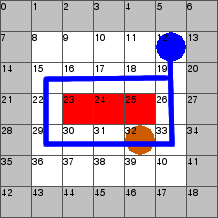
\includegraphics[scale=.33]{figs/7x7_liveness.png}
\begin{tikzpicture}[scale=0.9]
\draw[step=0.5cm,color=gray] (-1.5,-1.5) grid (1,1);
\filldraw[fill=blue,draw=black] (+0.75,+0.75) circle (0.2cm);
\filldraw[fill=red,draw=black] (0,0) rectangle (-0.5,-0.5);
\filldraw[fill=red,draw=black] (-0.5,0) rectangle (-1,-0.5);
\filldraw[fill=red,draw=black] (0,0) rectangle (0.5,-0.5);
\filldraw[fill=blue!40!white,draw=black] (+0.75,+0.75) circle (0.2cm);
\filldraw[fill=orange!40!white,draw=black] (0.25,-0.75) circle (0.2cm);
\draw[blue,thick] (-1.35,-0.75) rectangle (0.75,0.25);
\draw[blue,thick,->] (0.73,0.75) -> (0.75,0.25);
\node at (-1.30,+0.75) {\tiny{0}};
\node at (-0.80,+0.75) {\tiny{1}};
\node at (-0.30,+0.75) {\tiny{2}};
\node at (0.20,+0.75) {\tiny{3}};
\node at (0.73,+0.75) {\tiny{4}};
\node at (-1.35,+0.25) {\tiny{5}};
\node at (-0.85,+0.25) {\tiny{6}};
\node at (-0.35,+0.25) {\tiny{7}};
\node at (0.25,+0.25) {\tiny{8}};
\node at (0.75,+0.25) {\tiny{9}};
\node at (-1.35,-0.25) {\tiny{10}};
\node at (-0.85,-0.25) {\tiny{11}};
\node at (-0.35,-0.25) {\tiny{12}};
\node at (0.25,-0.25) {\tiny{13}};
\node at (0.75,-0.25) {\tiny{14}};
\node at (-1.35,-0.75) {\tiny{15}};
\node at (-0.85,-0.75) {\tiny{16}};
\node at (-0.35,-0.75) {\tiny{17}};
\node at (0.25,-0.75) {\tiny{18}};
\node at (0.75,-0.75) {\tiny{19}};
\node at (-1.35,-1.25) {\tiny{20}};
\node at (-0.85,-1.25) {\tiny{21}};
\node at (-0.35,-1.25) {\tiny{22}};
\node at (0.25,-1.25) {\tiny{23}};
\node at (0.75,-1.25) {\tiny{24}};
\end{tikzpicture}
\end{center}
\end{minipage}
\begin{minipage}{0.28\textwidth}
\vspace{0.1cm}
\caption{ Agent locations on an (infinite) path in the abstract counterexample graph from Example~\ref{ex:simple-liveness-counterex}. In the graph, the first node is labelled with $(4,\{18\})$, the second with $(9,\{Q_2\})$, and all other nodes with some $(l_a,\{Q_1,Q_2\})$.}
\label{fig:simple-liveness-counterex}
\end{minipage}

\end{figure}

\bigskip 

\begin{example}\label{ex:simple-liveness-counterex}
We saw in Example~\ref{ex:simple-safety-realizability} that in the safety surveillance game $(G,\LTLglobally p_2)$ the agent does not have a winning strategy. %This means, that the agent cannot ensure keeping at all times the uncertainty about the current position of the target to at most two positions.
We now consider a relaxed requirement, namely, that the uncertainty drops to at most $2$ infinitely often. We consider the liveness surveillance game 
$(G,\LTLglobally \LTLfinally p_2)$.

Let $\part = \{Q_1,Q_2\}$ be the partition from Example~\ref{ex:simple-safety-unconcretizable}. That is, $Q_1$, corresponds to the first two columns of the grid, and the set $Q_2$ contains the locations from the other three columns. 


Figure~\ref{fig:simple-liveness-counterex} shows an infinite path (in lasso form) in the abstract game $(\alpha_\part(G),\LTLglobally \LTLfinally p_2)$.  The figure depicts only the corresponding trajectory (sequence of positions) of the agent. The initial abstract state is $(4,\{18\})$, the second node on the path is labeled with the abstract state $(9,\{Q_2\})$, and all other nodes on the path are labeled with abstract states of the form $(l_a,\{Q_1,Q_2\})$ for some $l_a$. As each abstract state in the cycle violates $p_2$, the path violates $\LTLglobally \LTLfinally p_2$. The same holds for all infinite paths in the existing abstract counterexample graph.
\qed
\end{example}

\bigskip

A \emph{concrete counterexample graph} $\counterex_\belief$ for the belief game $(G_\belief,\LTLglobally\LTLfinally p_k)$ is defined analogously, with the difference that the nodes are now labelled with states in $S_\belief$.

An abstract counterexample graph $\counterex_\abstr$ for the game $(G_\abstr,\LTLglobally\LTLfinally p_k)$ is \emph{concretizable} if there exists a counterexample
$\counterex_\belief$ in $(G_\belief,\LTLglobally \LTLfinally p_k)$, such that for each infinite path $\pi_\abstr = v_\abstr^0,v_\abstr^1,\ldots$ starting from the initial node of $\counterex_\abstr$ there exists an infinite path $\pi_\belief = v_\belief^0,v_\belief^1,\ldots$ in $\counterex_\belief$ staring from its initial node such that if $v_\abstr^i$ is labelled with $(l_a,A_t)$ in $\counterex_\abstr$, then the corresponding node $v_\belief^i$ in $\counterex_\belief$ is labelled with $(l_a,B_t)$ for some $B_t \in \mathcal{P}(L)$ for which $B_t \subseteq \gamma(A_t)$.

Similarly to the set of trees associated with an abstract counterexample tree defined in the previous section, we can define a set of graphs $\graphs(\counterex_\abstr)$ of potential concretizations of $\counterex_\abstr$. In the remainder of this section we describe a procedure for constructing and analyzing one such graph, which will then have to be repeated for the different graphs.

Again, for the case of perfect sensing and no static sensors, the set of graphs contains a single graph. 
%\subsection{Counterexample-Guided Refinement}
%\subsubsection{Forward belief-set propagation}

To check if an abstract counterexample graph $\counterex_\abstr$ is concretizable, we construct a finite graph $\mathcal{D}$ whose nodes are labelled with elements of $\states_\belief$ and with nodes of $\counterex_\abstr$.
By construction we will ensure that if a node $d$ in $\mathcal D$ is labelled with $\langle(l_a,B_t),v \rangle$, where $(l_a,B_t)$ is a belief state, and $v$ is a node in $\counterex_\abstr$, then $v$ is labelled with $(l_a,A_t)$ in $\counterex_\abstr$, and $B_t \subseteq \gamma(A_t)$. 

Initially $\mathcal D$ contains a single node $d_0$ labelled with $\langle s_\belief^\init,v_0\rangle$, where $v_0$ is initial node of $\counterex_\abstr$. Consider a node $d$ in $\mathcal D$ labelled with $\langle(l_a,B_t),v \rangle$. For every child $v'$ of $v$ in $\counterex_\abstr$, labelled with an abstract state $(l_a',A_t')$ we proceed as follows. We select one belief set $B_t$ such that $((l_a,B_t),(l_a',B_t')) \in T_\belief$ and $B_t' \subseteq \gamma(A_t')$. If there exists a node $d'$ in $\mathcal D$ labelled with $\langle (l_a',B_t'),v\rangle$, then we add an edge from $d$ to $d'$ in $\mathcal{D}$. Otherwise, we create such a node and add the edge. We continue until no more nodes and edges can be added to $\mathcal D$. The procedure is guaranteed to terminate, since both  the graph $\counterex_\belief$, and $\states_\belief$ are finite, and we add a node labelled $\langle s_\belief, v\rangle$ to $\mathcal D$ at most once. Furthermore, the number of different graphs that we can construct in this way, by choosing different successor belief sets, is also finite. Thus, the set of graphs $\graphs(\counterex_\abstr)$ is also finite.

If every graph $\mathcal D$ in $\graphs(\counterex_\abstr)$ contains a reachable cycle (it suffices to consider simple cycles, i.e., without repeating intermediate nodes) $\rho = d_0,\ldots,d_n$ with $d_0 = d_n$ such that some $d_i$ is labelled with $(l_a,B_t)$ where $(l_a,B_t) \models p_k$, then we can conclude that the abstract counterexample $\counterex_\abstr$ is not concretizable. If for some graph $\mathcal D$ no such cycle exists, then $\mathcal D$ is a concrete counterexample graph for $(G_\belief,\LTLglobally\LTLfinally p_k)$. 

%\comment{
\begin{algorithm}[h!] 
%\small
%\vspace{-.5cm}
\KwIn{liveness surveillance game $(G,\LTLglobally\LTLfinally p_k)$, \newline 
abstract counterexample graph $\counterex_\abstr$ with initial node $v_0$}
\KwOut{a path $\pi$ in a graph $\mathcal D$ or {\sc concretizable}}

\smallskip

let $\mathcal D = (D,E)$ be a graph with\\
nodes $D := \{d_0\}$ and edges $E := \emptyset$\;

\smallskip

annotate $d_0$ with $\langle s_\belief^\init, v_0\rangle$\; 

\SetKwRepeat{Do}{do}{while}

\Do{$\mathcal D \neq \mathcal D'$}{
$\mathcal D' := \mathcal D$\;
 \ForEach{node $d$ in $\mathcal D$ labelled with $\langle(l_a,B_t),v\rangle$}{
  \ForEach{child $v'$ of $v$ in $\counterex_\abstr$ labelled $(l_a',A_t')$}{
  let $B_t$ be such that $B_t' \subseteq \gamma(A_t')$ and $((l_a,B_t),(l_a',B_t')) \in T_\belief$\;
  \eIf{there is a node $d' \in D$ labelled with $\langle (l_a',B_t'),v'\rangle$}{add an edge $(d,d')$ to $E$}
  {add a node $d'$ labelled $\langle (l_a',B_t'),v'\rangle$\;
  add an edge $(d,d')$ to $E$}
}
}
}
\leIf{there is a lasso path $\pi$ in $\mathcal D$ starting from $d_0$ such that some node in the cycle is annotated with $\langle s_\belief,v\rangle$ and $s_\belief\models p_k$}
{\KwRet{$\pi$;}\newline}
{\KwRet{{\sc concretizable}}}

\smallskip

\caption{Analysis of abstract counterexample graphs for games with liveness surveillance objectives.}
\label{algo:cex-analysis-liveness}
\end{algorithm}
%}


\bigskip 

\begin{example}\label{ex:simple-liveness-unconcretizable}
The abstract counterexample graph in the game $(\alpha_\part(G),\LTLglobally \LTLfinally p_2)$ discussed in Example~\ref{ex:simple-liveness-counterex} is not conretizable, since for the path in the abstract graph depicted in Figure~\ref{fig:simple-liveness-counterex} there exists a corresponding path in the unique graph $\mathcal D$ with a node in the cycle labelled with a set in $G_\belief$ that satisfies $p_2$. More precisely, the cycle in the graph $\mathcal D$ contains a node labelled with $(19,\{10\})$. Intuitively, as the agent moves from the upper to the lower part of the grid along this path, upon not observing the target, it can infer from the sequence of observations that the only possible location of the target is $10$. Thus, this infinite path is winning for the agent.
\qed
\end{example}

\bigskip 

\begin{theorem}
If for some graph $\mathcal{D}$ in $\graphs(\counterex_\abstr)$  Algorithm~\ref{algo:cex-analysis-liveness} returns {\sc concretizable}, then $\counterex_\abstr$ is concretizable. Otherwise, if for every graph $\mathcal D$ in $\graphs(\counterex_\abstr)$ it returns path $\pi$ in $\mathcal D$, then $\counterex_\abstr$ is not concretizable.
\end{theorem}
{\it Proof.}\ \ 
By applying Algorithm~\ref{algo:cex-analysis-liveness} in order to analyze all graphs in $\graphs(\counterex_\abstr)$, we check for each such graph if it is a concrete counterexample graph, that is, for each of its lasso paths the every state in the loop of that path violates $p_k$. By definition, Algorithm~\ref{algo:cex-analysis-liveness} returns {\sc concretizable} precisely when this is the case, that is when $\counterex_\abstr$ is concretizable. If for each graph in $\graphs(\counterex_\abstr)$ the algorithm returns a lasso path $\pi$ for which every state in its loop violates $p_k$, then this path demonstrates that the corresponding graph is not a concrete counterexample. If this is the case for all graphs in $\graphs(\counterex_\abstr)$, then $\counterex_\abstr$ is indeed spurious.
\qed

\bigskip 

\subsubsection{Backward partition splitting}

Consider a path in a graph $\mathcal{D}\in\graphs(\counterex_\abstr)$ of the form $\pi = d_0,\ldots, d_n,d_0',\ldots,d_m'$ where $d_n = d_m'$, and where for some $0 \leq i \leq m$ for the label $(l_a^i,B_t^i)$ it holds that $(l_a^i,B_t^i) \models p_k$. Let 
$\pi_\abstr = v_0,\ldots, v_n,v_0',\ldots,v_m'$ be the sequence of nodes in $\counterex_\abstr$ corresponding to the labels in $\pi$. By construction of $\mathcal D$, $\pi_\abstr$ is a path in $\counterex_\abstr$ and $v_n = v_m'$. We apply the refinement procedure from Algorithm~\ref{algo:refinement-safety} to the whole path $\pi_\abstr$, as well as to the path-prefix $v_0,\ldots, v_n$.


Let $\part$ and $\part'$ be two counterexample partitions such that $\part' \preceq \part$. Let $\counterex_\abstr$ be an abstract counterexample graph in $(\alpha_\part(G),\LTLglobally\LTLfinally p_k)$. We define $\gamma_{\part'}(\counterex_\abstr)$ to be the set of abstract counterexample graphs in $(\alpha_{\part'}(G),\LTLglobally\LTLfinally p_k)$ such that for every infinite path $\pi$ in $\counterex_\abstr'$ there exists an infinite path $\pi$ in $\counterex_\abstr$ such that for every node in $\pi'$ labelled with $(l_a,A_t')$ the corresponding node in $\counterex_\abstr$ is labelled with an abstract state $(l_a,A_t)$ such that $\gamma(A_t') \subseteq \gamma(A_t)$.


\bigskip 

\begin{theorem}If $\part'$ is the partition 
obtained by refining $\part$ with respect to all graphs in the set $\graphs(\counterex_\abstr)$ for an unconcretizable abstract counterexample $\counterex_\abstr$ in $(\alpha_\part(G),\LTLglobally\LTLfinally p_k)$, then $\gamma_{\part'}(\counterex_\abstr) = \emptyset$, and also $\gamma_{\part''}(\counterex_\abstr) = \emptyset$ for every partition $\part''$ with $\part'' \preceq \part'$.
\end{theorem}
{\it Proof.}\ \ 
Let $\part'$ be the partition obtained by refining $\part$ with respect to all the graphs in $\graphs(C_\abstr)$ for an unconcretizable abstract counterexample $\counterex_\abstr$ in $(\alpha_\part(G),\LTLglobally\LTLfinally p_k)$.

For every graph in $\graphs(C_\abstr)$ and corresponding infinite path $(l_a^0,B_t^0)(l_a^1,B_t^1)\ldots$ represented as lasso, with which we have refined the abstraction, every abstract partition $\part'' \preceq \part'$, and every infinite lasso path $(l_a^0,A_t^0) (l_a^1,A_t^1)\ldots$ in $\alpha_{\part''}(G)$ with $\alpha_{\part''}(B_t^i) = A_t^i$ we have that $\widetilde A_t^j \models p_k$ for infinitely many $j$. That is, the performed refinement ensures that in every finer abstraction, the abstraction of the paths with respect to which the partition was refined is precise enough to ensure that the safety property is not violated on this path.

Now, assume for the sake of contradiction that $\gamma_{\part''}(\counterex_\abstr) \neq \emptyset$, and let $\counterex_\abstr'' \in\gamma_{\part''}(\counterex_\abstr)$. By the definition of $\gamma$ and $\graphs$, we have that there exists a graph $D$ in $\graphs(\counterex_\abstr)$ that is also an element of $\graphs(\counterex_\abstr'')$. Thus, for some $(l_a^0,B_t^0)\ldots (l_a^m,B_t^m)$ in $D$ with respect to which we have refined the abstraction, it holds that $(l_a^0,\alpha_{\part''}(B_t^0)) (l_a^1,\alpha_{\part''}(B_t^1))\ldots$ is an infinite path represented as lasso in $\counterex_\abstr''$. By the property above, we have $\alpha(B_t^i)\models p_k$ for infinitely many $i$, which contradicts to the choice of $\counterex_\abstr''$ as a counterexample in $\alpha_{\part''}(G)$. This concludes the proof that $\gamma_{\part''}(\counterex_\abstr) = \emptyset$.
\qed
\bigskip 

\begin{example}\label{ex:simple-liveness-refinement}
We refine the abstraction partition $\part$ from Example~\ref{fig:simple-liveness-counterex} using the path identified in Example~\ref{ex:simple-liveness-counterex}, in order to eliminate the abstract counterexample. For this, following the refinement algorithm, we first split the set $Q_1$ into sets $Q_1' = \{10\}$ and $Q_2' = Q_1 \setminus \{10\}$, and let $Q_3' = Q_2$. However, since from some locations in $Q_2'$ and in $Q_3'$ the target can reach locations in $Q_2'$ and $Q_3'$, in order to eliminate the counterexample, we need to propagate the refinement backwards along the path and split $Q_2'$ and $Q_3'$ further. With that, we obtain an abstraction partition with $10$ sets, which is guaranteed to eliminate this abstract counterexample. In fact, in this example this abstraction turns out to be sufficiently precise to obtain a winning strategy for the agent.
\qed
\end{example}

%
%%%%%%%%%%%%%%%%%%%%%%%%%%%%%%%%%%%%%%%%%%%%%%%%%%%%%%%%%%%%%%%%%%%%%%%%%%%%%%%%%
%
\section{BELIEF REFINEMENT FOR GENERAL SPECIFICATIONS}% SURVEILLANCE OBJECTIVES}
%
%\subsection{General Surveillance and Task Specifications}
%We have described refinement procedures for safety and liveness surveillance objectives. If we are given a conjunction of such objectives, we first apply the refinement procedure for safety, and if no path for which we can refine is found, we then apply the refinenment procedure for liveness. 

In the general case, we check if the counterexample contains a state for which the concrete belief is a strict subset of the abstract one. If this is not the case, then the counterexample is concretizable, otherwise we refine the abstraction to make this belief precise. In the special case when we have a conjunction of a surveillance and task specifications, we first refine with respect to the surveillance objective as described above, and if this is not possible, with respect to such a node. Since the set of states in the game is finite, the iterative refinement will terminate, either with a concretizable counterexample, or with a surveillance strategy.  


%\begin{itemize}
%\item $\LTLglobally p_k \wedge \LTLglobally\LTLfinally p_l$: first check concretizability of all paths in the graph to states violating the safety constraints, if one is not concretizable then done, if all are concretizable, then apply method for liveness.
%\item General surveillance objectives: refine for some node where the true belief is more precise than the abstract one. not guaranteed to eliminate counterexample, but refinement loop guaranteed to still terminate since system is finite state and a proper split is done at each step. heuristics for identifying such nodes.
%\item $\varphi_{\mathit{surveillance}} \wedge \varphi_{\mathit{task}}$  if surveillance is a conjunction of safety and liveness, then in sequence: safety, liveness, task; otherwise as previous item.
%\item Full specification language: as for general surveillance.
%\end{itemize}

%\subsection{Discussion on Abstraction Refinement}
%As we have shown, the iterative abstraction refinement procedure we have described is guaranteed to terminate with either a winning strategy for the agent or with a concrete counterexample. In theory, a user can start with a very uninformed abstraction (for example, a trivial abstraction with one abstraction partition consisting of the entire state space), and the counterexample-guided refinement procedure will eventually terminate with an abstraction and a corresponding strategy. In practice, however, it is advisable to start with a suitably chosen informed abstraction, in order to reduce the number of necessary refinement iterations. In the next section we show some examples of user-provided abstractions which even require no refinement at all. Furthermore, user-provided abstractions are oftentimes 
more `intuitive' compared to the ones generated by the automated refinement procedure.

Ideally, constructing a suitable initial abstraction should be automated as well. However, abstractions are highly dependent on the sensor function and the structure of the environment. The process of generating initial abstractions based on automatically identified map features is on-going work. 
%%%%%%%%%%%%%%%%%%%%%%%%%%%%%%%%%%%%%%%%%%%%%%%%%%%%%%%%%%%%%%%%%%%%%%%%%%%%%%%%%
%
\section{EXPERIMENTAL EVALUATION ON GRIDWORLD}\label{sec:experiments}
In this section we report on the application of the proposed method for surveillance strategy synthesis on gridworld-based examples. The purpose of the experimental evaluation is to highlight the following key points:
\begin{itemize}
    \item The effect of different abstractions on the evolution of the belief sets of the agent.
    \item Sequences of abstractions resulting from automated abstraction refinement.
    \item The qualitative differences in the agent's behaviour resulting from surveillance strategies synthesized for different types of specifications.
\end{itemize}


We apply the \texttt{slugs} reactive synthesis tool~\cite{EhlersR16} to the abstract surveillance games in order to synthesize the surveillance strategies. The experiments were performed on an Intel i5-5300U 2.30 GHz CPU with 8 GB of RAM. 

\subsection{Effect of Abstractions on Belief}
The aim of this experiment is to illustrate the effect of different abstractions (generated using different abstraction partitions) on the evolution of belief sets. Naturally, the finer the abstraction, the slower the growth of the size of the belief set over time, and hence the easier it is to satisfy the specification. However, the increased precision of the abstraction comes at the cost of increased synthesis time. 

Figure~\ref{fig:case1} shows a gridworld divided into 7 abstraction partitions. The surveillance objective requires the agent to infinitely often know precisely the location of the target (either see it, or have a belief consisting of one cell). Additionally, it has to perform the task of patrolling (visiting infinitely often) the green 'goal' cell. Formally, the specification is $\LTLglobally\LTLfinally p_1 \wedge \LTLglobally\LTLfinally \mathit{goal}$. The agent can move up to 3 grid cells away at each step. The sensor mode, that is, the observation function, used here is 'line-of-sight' with a range of 5 cells. The agent cannot see through obstacles (shown in red) and cannot see farther than 5 cells away.  We assume in this example that we have perfect sensing i.e., when the target is sensed, the agent knows its true location. There are no static sensors. 


\begin{figure}
\subfloat[Gridworld with a user-provided abstraction partition with 7 sets, marked by the thick black lines. \label{fig:case1}]{
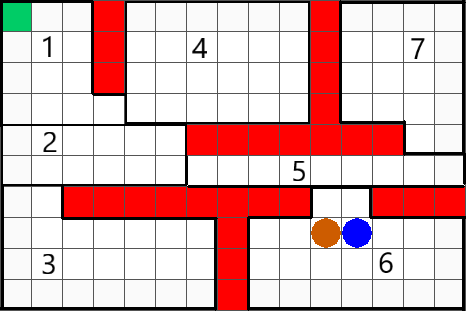
\includegraphics[width=0.45\linewidth]{Surveillance/figs/Liveness_part.png}
}
\hfill
\subfloat[Gridworld showing visibility of the agent. All locations shown in black are invisible to the agent. \label{fig:case1vis}]{
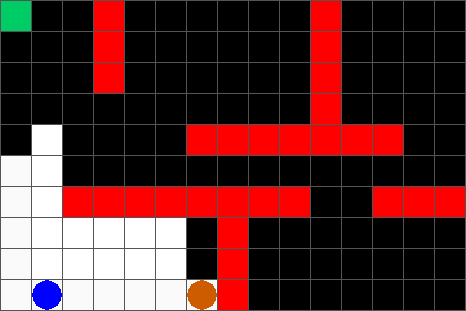
\includegraphics[width=0.45\linewidth]{Surveillance/figs/Liveness_t1.png}
}

\caption{10x15 gridworld with a liveness surveillance specification. The agent is depicted in blue, and the target in orange. The red locations are obstacles.}
\label{fig:casestudies1}

\end{figure}



\begin{figure}
\begin{minipage}{5.0cm}
	\centering
		\subfloat[$t_1$ \label{fig:case1t2}]{
		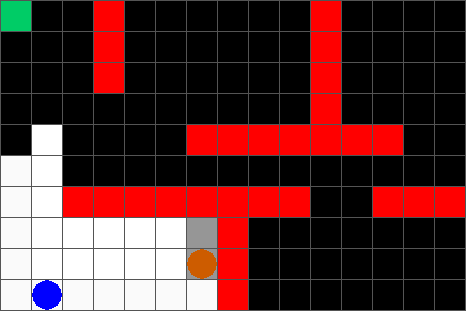
\includegraphics[width=0.47\linewidth]{Surveillance/figs/Liveness_t2.png}\hspace{.5cm}
	}
	\subfloat[$t_3$ \label{fig:case1t3}]{
		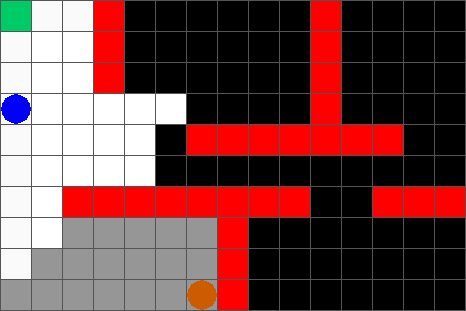
\includegraphics[width=0.47\linewidth]{Surveillance/figs/Liveness_t3.png}\hspace{.5cm}
	}
	\subfloat[$t_4$ \label{fig:case1t4}]{
	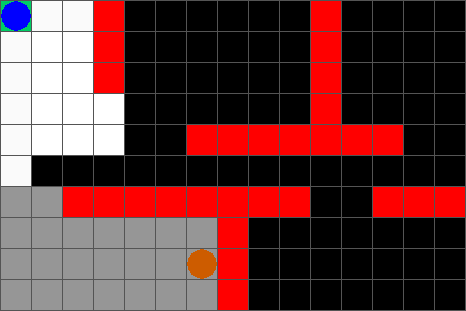
\includegraphics[width=0.47\linewidth]{Surveillance/figs/Liveness_t4.png}\hspace{.5cm}
}
\end{minipage}
\begin{minipage}{5.0cm}
	\centering
	\subfloat[$t_5$  \label{fig:case1t5}]{
		\includegraphics[width=0.47\linewidth]{Surveillance/figs/Liveness_t5.png}\hspace{.5cm}
	}
	\subfloat[$t_6$ \label{fig:case1t6}]{
		\includegraphics[width=0.47\linewidth]{Surveillance/figs/Liveness_t6.png}\hspace{.5cm}
	}
	\subfloat[$t_7$ \label{fig:case1t7}]{
		\includegraphics[width=0.47\linewidth]{Surveillance/figs/Liveness_t7.png}\hspace{.5cm}
	}
	
\end{minipage}

	
	\caption{Evolution of the agent's belief about the target's location as it moves towards the goal and loses sight of the target. Grey cells represent the locations the agent believes the target could be in. We show the belief at different timesteps $t_1,\ldots,t_7$ (note that $t_2$ is excluded for space concerns)
		}
	\label{fig:case1exp}
	
\end{figure}

Figure \ref{fig:case1exp} shows how the belief of the agent (shown in grey) can grow quickly when it cannot see the target. This growth occurs due to the coarseness of the abstraction, which overapproximates the target's true location. In 7 steps, the agent believes the target can be anywhere in the grid that is not in its vision. It has to then find the target in order to satisfy the surveillance requirement. Figure \ref{fig:search} illustrates the searching behaviour of the agent when it is trying to lower the belief below the threshold in order to satisfy the liveness specification. This  behaviour contrasts with the behaviour under safety surveillance considered later. A video of the simulation can be found at \url{http://goo.gl/YkFuxr}.

\begin{figure}

	\begin{minipage}{5.0cm}
		\centering
		\subfloat[$t_5$ \label{fig:search1}]{
			\includegraphics[width=0.47\linewidth]{Surveillance/figs/search_t2.png}\hspace{.5cm}
		}
		\subfloat[$t_7$ \label{fig:search2}]{
			\includegraphics[width=0.47\linewidth]{Surveillance/figs/search_t3.png}\hspace{.5cm}
		}
		\subfloat[$t_9$ \label{fig:search3}]{
			\includegraphics[width=0.47\linewidth]{Surveillance/figs/search_t4.png}\hspace{.5cm}
		}
	\end{minipage}
	\caption{The agent has to search for the target in order to lower its belief below the surveillance liveness specification.
	}
	\label{fig:search}
	
\end{figure}

In this example, an abstraction partition of size 7 was enough to guarantee the satisfaction of the surveillance specification.  For the purpose of comparison, we also solve the game with  an abstraction partition of size 12  to illustrate the change in belief growth. Figure \ref{fig:case1fineexp} shows the belief states growing much more slowly as the abstract belief states are smaller, and thus they more closely  approximate the true belief.
\begin{figure}

	\begin{minipage}{5.0cm}
		\centering
		\subfloat[$t_1$ \label{fig:casefine1t2}]{
			\includegraphics[width=0.47\linewidth]{Surveillance/figs/Liveness_t1.png}\hspace{.5cm}
		}
		\subfloat[$t_3$ \label{fig:case1finet3}]{
			\includegraphics[width=0.47\linewidth]{Surveillance/figs/Liveness_fine_t11.png}\hspace{.5cm}
		}
		\subfloat[$t_4$ \label{fig:case1finet4}]{
			\includegraphics[width=0.47\linewidth]{Surveillance/figs/Liveness_fine_t2.png}\hspace{.5cm}
		}
	\end{minipage}
	\begin{minipage}{5.0cm}
		\centering
		\subfloat[$t_5$  \label{fig:case1finet5}]{
			\includegraphics[width=0.47\linewidth]{Surveillance/figs/Liveness_fine_t3.png}\hspace{.5cm}
		}
		\subfloat[$t_6$ \label{fig:case1finet6}]{
			\includegraphics[width=0.47\linewidth]{Surveillance/figs/Liveness_fine_t4.png}\hspace{.5cm}
		}
		\subfloat[$t_7$ \label{fig:case1finet7}]{
			\includegraphics[width=0.47\linewidth]{Surveillance/figs/Liveness_t5.png}\hspace{.5cm}
		}
		
	\end{minipage}
	
	
	\caption{Evolution of the agent's belief about the target's location in a game  with an abstraction partition of size 12.
	}
	\label{fig:case1fineexp}
	
\end{figure}


The additional abstraction partitions result in a much larger game as the state space grows exponentially in the size of the abstraction partition. We compared the sizes of two abstract games for the 15x10 gridworld shown in Figure \ref{fig:casestudies1}, and the time it takes to synthesize a surveillance strategy in each of them. For an abstraction partition of size 7 the abstract game has 41700 states, and the synthesis time is 237s. In comparison, for an abstraction partition of size 13 the size of the abstract game is 636900 and the synthesis time is 810s. In contrast, the concrete belief-set game will have in the order of $2^{150}$ states, which is a state-space size that state-of-the-art synthesis tools cannot handle. 

%Table \ref{tab:exp1} compares the sizes of the corresponding abstract games, and the time it takes to synthesize a surveillance controller in each case.


%\begin{table}[h!]
%	\centering
%	\begin{tabular}{c|c|c}
%	Size of abstraction partition & Size of abstract game & Synthesis time \\ \hline \hline
%		7 & 41700 & 237s \\ 
%		12 & 636900 & 810s \\ 
%	\end{tabular}\caption{Comparison of synthesis times for coarse and fine abstractions on a 15x10 gridworld shown in Figure \ref{fig:casestudies}} \label{tab:exp1}
%\end{table}




\subsection{Automated Abstraction Refinement}
We now present an experiment to demonstrate the working of abstraction refinement procedure. 


\begin{figure}
\subfloat[User-provided initial abstraction. \label{fig:case1_autopart_before}]{\begin{tikzpicture}[scale=1]
\draw[step=0.5cm,color=gray] (-3.5,-2) grid (3,2);


\filldraw[fill=green,draw=black] (-3.5,2) rectangle (-3,1.5);
% \filldraw[fill=red,draw=black] (-2.5,2) rectangle (-2,1.5);
\filldraw[fill=red,draw=black] (-2.5,2) rectangle (-2,1.0);
\filldraw[fill=red,draw=black] (1,2) rectangle (1.5,0.0);
\filldraw[fill=red,draw=black] (-1,0.5) rectangle (2.5,0.0);
\filldraw[fill=red,draw=black] (2,-0.5) rectangle (3,-1.0);
\filldraw[fill=red,draw=black] (-2,-0.5) rectangle (1,-1.0);
\filldraw[fill=red,draw=black] (-0.5,-1.0) rectangle (0,-2.0);

\filldraw[fill=none,draw=blue,line width=0.6mm] (-3.5,2.0) rectangle (-2.5,-2.0);
\draw[black, line width = 0.6mm] plot coordinates{(-2.0,2) (-2.0,1) (-2.5,1) (-2.5,-2) (-0.5,-2) (-0.5,-1) (-2.0,-1) (-2.0,-0.5) (3.0,-0.5) (3.0,-0.0) (-1.0,-0.0) (-1.0,0.5) (1.0,0.5) (1.0,2)}--cycle;
\draw[cyan, line width = 0.6mm] plot coordinates{(0,-1.0) (0,-2.0) (3,-2.0) (3,-1.0) (2,-1.0) (2,-0.5) (1,-0.5) (1,-1.0)}--cycle;
\draw[magenta, line width = 0.6mm] plot coordinates{(1.5,2.0) (1.5,0.5) (2.5,0.5) (2.5,0.0) (3.0,0.0) (3.0,2.0)}--cycle;
% \filldraw[fill=blue!40!white,draw=black] (+0.75,+0.75) circle (0.2cm);
% \filldraw[fill=orange!40!white,draw=black] (0.25,-0.75) circle (0.2cm);
\node at (-3.0,+0.0) {\normalsize{\textbf{$Q_1$}}};
\node at (-1.5,-0.0) {\normalsize{\textbf{$Q_2$}}};
\node at (2.25,1.25) {\normalsize{\textbf{$Q_3$}}};
\node at (1.5,-1.5) {\normalsize{\textbf{$Q_4$}}};
% \node at (-1.5,-0.0) {\large{\textbf{2}}};
% \node at (-0.30,+0.75) {\tiny{2}};
% \node at (0.20,+0.75) {\tiny{3}};
% \node at (0.73,+0.75) {\tiny{4}};
% \node at (-1.33,+0.25) {\tiny{5}};
% \node at (-0.85,+0.25) {\tiny{6}};
% \node at (-0.35,+0.25) {\tiny{7}};
% \node at (0.25,+0.25) {\tiny{8}};
% \node at (0.75,+0.25) {\tiny{9}};
% \node at (-1.28,-0.27) {\tiny{10}};
% \node at (-0.78,-0.27) {\tiny{11}};
% \node at (-0.28,-0.27) {\tiny{12}};
% \node at (0.28,-0.27) {\tiny{13}};
% \node at (0.75,-0.25) {\tiny{14}};
% \node at (-1.3,-0.75) {\tiny{15}};
% \node at (-0.8,-0.75) {\tiny{16}};
% \node at (-0.3,-0.75) {\tiny{17}};
% \node at (0.25,-0.75) {\tiny{18}};
% \node at (0.75,-0.75) {\tiny{19}};
% \node at (-1.27,-1.25) {\tiny{20}};
% \node at (-0.8,-1.25) {\tiny{21}};
% \node at (-0.3,-1.25) {\tiny{22}};
% \node at (0.25,-1.25) {\tiny{23}};
% \node at (0.75,-1.25) {\tiny{24}};
\end{tikzpicture}}
%\hfill
\subfloat[Refined abstraction.\label{fig:refined-abstraction}]{
\begin{tikzpicture}[scale=1]
\draw[step=0.5cm,color=gray] (-3.5,-2) grid (3,2);


\filldraw[fill=green,draw=black] (-3.5,2) rectangle (-3,1.5);
% \filldraw[fill=red,draw=black] (-2.5,2) rectangle (-2,1.5);
\filldraw[fill=red,draw=black] (-2.5,2) rectangle (-2,1.0);
\filldraw[fill=red,draw=black] (1,2) rectangle (1.5,0.0);
\filldraw[fill=red,draw=black] (-1,0.5) rectangle (2.5,0.0);
\filldraw[fill=red,draw=black] (2,-0.5) rectangle (3,-1.0);
\filldraw[fill=red,draw=black] (-2,-0.5) rectangle (1,-1.0);
\filldraw[fill=red,draw=black] (-0.5,-1.0) rectangle (0,-2.0);

\filldraw[fill=none,draw=blue,line width=0.6mm] (-3.5,2.0) rectangle (-2.5,-2.0);
\draw[black, line width = 0.6mm] plot coordinates{(-2.0,2) (-2.0,1) (-2.5,1) (-2.5,-2) (-0.5,-2) (-0.5,-1) (-2.0,-1) (-2.0,-0.0) (-1.0,-0.0) (-1.0,0.5) (1.0,0.5) (1.0,2)}--cycle;
\draw[cyan, line width = 0.6mm] plot coordinates{(0,-1.0) (0,-2.0) (3,-2.0) (3,-1.0) (2,-1.0) (2,-0.5) (1,-0.5) (1,-1.0)}--cycle;


\filldraw[fill=none,draw=teal, line width=0.6mm] (-2.0,0.0) rectangle (-0.0,-0.5);
\filldraw[fill=none,draw=violet, line width=0.6mm] (-0.0,0.0) rectangle (1.0,-0.5);
\filldraw[fill=none,draw=lime, line width=0.6mm] (1.0,0.0) rectangle (3.0,-0.5);
\draw[brown, line width = 0.6mm] plot coordinates{(2.0,2.0) (2.0,1.0) (2.5,1.0) (2.5,0.0) (3.0,0.0) (3.0,2.0)}--cycle;
\draw[gray, line width = 0.6mm] plot coordinates{(1.5,2.0) (1.5,0.5) (2.5,0.5) (2.5,1.0) (2.0,1.0) (2.0,2.0)}--cycle;
\draw[darkgray, line width = 0.6mm] plot coordinates{(2.0,-1.0) (2.0,-1.5) (2.5,-1.5) (2.5,-2.0) (3,-2.0) (3,-1)}--cycle;


% \filldraw[fill=blue!40!white,draw=black] (+0.75,+0.75) circle (0.2cm);
% \filldraw[fill=orange!40!white,draw=black] (0.25,-0.75) circle (0.2cm);
\node at (-3.0,+0.0) {\textbf{$Q_1$}};
\node at (-1.25,-0.25) {\normalsize{\textbf{$Q_3$}}};
\node at (-1.0,1.25) {\normalsize{\textbf{$Q_2$}}};
\node at (1.5,-1.5) {\normalsize{\textbf{$Q_8$}}};
\node at (0.5,-0.25) {\normalsize{\textbf{$Q_4$}}};
\node at (2.0,-0.25) {\normalsize{\textbf{$Q_5$}}};
\node at (1.8,0.75) {\normalsize{\textbf{$Q_6$}}};
\node at (2.75,1.25) {\normalsize{\textbf{$Q_7$}}};
\node at (2.5,-1.25) {\normalsize{\textbf{$Q_9$}}};
% \node at (-1.5,-0.0) {\large{\textbf{2}}};
% \node at (-0.30,+0.75) {\tiny{2}};
% \node at (0.20,+0.75) {\tiny{3}};
% \node at (0.73,+0.75) {\tiny{4}};
% \node at (-1.33,+0.25) {\tiny{5}};
% \node at (-0.85,+0.25) {\tiny{6}};
% \node at (-0.35,+0.25) {\tiny{7}};
% \node at (0.25,+0.25) {\tiny{8}};
% \node at (0.75,+0.25) {\tiny{9}};
% \node at (-1.28,-0.27) {\tiny{10}};
% \node at (-0.78,-0.27) {\tiny{11}};
% \node at (-0.28,-0.27) {\tiny{12}};
% \node at (0.28,-0.27) {\tiny{13}};
% \node at (0.75,-0.25) {\tiny{14}};
% \node at (-1.3,-0.75) {\tiny{15}};
% \node at (-0.8,-0.75) {\tiny{16}};
% \node at (-0.3,-0.75) {\tiny{17}};
% \node at (0.25,-0.75) {\tiny{18}};
% \node at (0.75,-0.75) {\tiny{19}};
% \node at (-1.27,-1.25) {\tiny{20}};
% \node at (-0.8,-1.25) {\tiny{21}};
% \node at (-0.3,-1.25) {\tiny{22}};
% \node at (0.25,-1.25) {\tiny{23}};
% \node at (0.75,-1.25) {\tiny{24}};
\end{tikzpicture}
}
\caption{Experiment showcasing automated abstraction refinement in a 13$\times$8 gridworld. The user-provided abstraction of 4 abstract states shown in ~\ref{fig:case1_autopart_before} is refined further into 9 abstract states shown in~\ref{fig:refined-abstraction}.}
\label{fig:case1_autopart}
\end{figure}



Starting with an abstract game generated by a partition with four elements shown in Figure~\ref{fig:case1_autopart_before}, the refinement algorithm terminates after 5 iterations (with total running time of 821 s). The resulting partition $\mathcal{Q} = \{Q_1,...,Q_9 \}$ has $9$ elements shown as the numbered regions in Figure~\ref{fig:refined-abstraction}.

This experiment shows that, in general, we do not guarantee that the abstraction generated by the refinement approach is necessarily the smallest possible. A handcrafted partitioning in the same environment shown in the previous section was able to produce a winning strategy with 7 abstract belief states instead of 9. Although the abstraction refinement algorithm is always guaranteed to terminate, in general, the user-provided initial abstraction has a significant effect on the number of abstract belief states of the resulting abstraction. It is thus important to combine initial user-provided abstractions, that are crafted as well as possible, with the automated refinement that eliminates any remaining imprecision that was not accounted for by the user.

 



%\Suda{Not sure if we should keep this next part}
\subsection{Discussion}
 The difference in the behaviour in the case studies highlights the different use cases of the surveillance objectives. Depending on the domain, the user can specify a combination of safety and liveness specification to tune the behaviour of the agent. In a critical surveillance situation (typical in defense or security situations), the safety specification will guarantee to the user that the belief will never grow too large. However, in less critical situations (such as luggage carrying robots in airports), the robot has more flexibility in allowing the belief to grow as long as it can guarantee its reduction in the future. 
%
%%%%%%%%%%%%%%%%%%%%%%%%%%%%%%%%%%%%%%%%%%%%%%%%%%%%%%%%%%%%%%%%%%%%%%%%%%%%%%%%%
%
\section{SECURITY APPLICATION CASE STUDY}
%
In this section, we demonstrate the effectiveness of the proposed framework to a case study for an urban security application with high-fidelity simulated sensors and robots. 
%Physical security applications typically require the housing and protection of sensitive materials or locations. Often, such environments are large and it is difficult to have complete surveillance coverage at all times using only static sensors. In such situations, deploying an autonomous mobile agent with sensing capabilities can greatly reduce coverage requirements from static sensors. When utilizing autonomous agents it is necessary to provide quantitative guarantees on their belief of the location of an intruding target in order to direct security measures accurately. The method proposed in this paper generates strategies for fully autonomous surveillance with quantitative guarantees on the size of the belief of the target's location and hence is a natural fit for security applications. 
We provide the code for the implementation on Github\footnote{Github: \url{https://github.com/u-t-autonomous/Surveillance}} and the videos for all simulations at the corresponding Github page \footnote{Github page: \url{https://u-t-autonomous.github.io/Surveillance-Synthesis/}}.
%We will use the case study to demonstrate the versatility and applicability of our surveillance strategy and belief abstraction methods across multiple high-fidelity simulation environments.

% \subsection{Combating poaching}
% First, consider the problem of tracking poachers in Africa. 
% UAVs are increasingly being adopted for monitoring of illegal hunting and poaching \cite{poaching}. In countries such as Kenya \cite{poaching}, South Africa, and Zimbabwe \cite{drones}, drones have been deployed and tested in an attempt to reduce poaching by providing constant surveillance \cite{poaching}. However, all of these solutions still require a pilot to remotely operate the UAV or manually provide it waypoints. In this paper we propose a method to generate strategies that can allow for \emph{fully autonomous surveillance} with quantitative guarantees on the \emph{belief in the position of the target}. These quantitative guarantees allow a response to be effectively mobilized by relevant authorities. 

% We simulate a jungle environment using Unreal Engine 4 as shown in Figure \ref{fig:UE4JungleProto} and UAVs are simulated in the environment using an Airsim plugin \cite{airsim}. In Section VII we present simulations of an autonomous UAV performing surveillance mission in this environment. 

% \begin{figure}[h]
%     \centering
%     \includegraphics[width = 0.9\linewidth]{figs/UE4JungleProto.png}
%     \caption{Unreal Engine 4 Jungle Environment}
%     \label{fig:UE4JungleProto}
% \end{figure}
%\subsection{Security}



% \begin{figure}[h]
%     \centering
%     \includegraphics[width = 3 in]{figs/GazArena.png}
%     \caption{Gazebo Environment}
%     \label{fig:GazArena}
% \end{figure}

%andia National Labs considers examples where there is a compound that has a sensitive area that must be protected and is surrounded by land that contains wild life. Sometimes when an intruder is detected, the security system cannot determine if the threat is real or if there is simply an animal wandering around. A security officer must then go out and find the intruder to determine the state of the threat. In order to reduce wasted time, actively tracking that threat to provide the security personnel with a small region to search instead of a last known location saves resources. 

%and of security around a sensitive compound where tracking potential intruders is required for security personnel to make contact with and determine if the threat is real or false.




\subsection{Robot Platforms}

We use two robot simulation platforms to demonstrate the generality and applicability of the platform-agnostic methodology developed in this paper:
\begin{enumerate}
    \item An Iris quadcopter, which uses the PX4 flight stack and is capable of waypoint control.
    \item Stanley Innovations segway, which uses the ROS navigation stack for mapping, waypoint control, and autonomous obstacle avoidance. 
\end{enumerate}
To simulate the sensor output, we directly access the ground truth position of the moving target and add noise. We model the sensor and state estimation uncertainty as described in section \ref{sec:sensefunction} using a simulated 360 degree LiDAR with range of  $10$ meters, angular resolution of 1 degree, range accuracy of $\pm 3$ cm.


The function $vis$ is built directly from the sensor range parameter. To construct the function $sense$ we use a worst-case conservative Gaussian noise model. Given a sensor measurement, let $0 \leq p(l) \leq 1$ be the probability the target is in location $l$. We construct the uncertainty set $U$ of possible target states for each sensor measurement $sense(l_a,l_t)$ by including all states with a probability greater than $\delta$ where $0\leq \delta \leq 1$ can be set by the user. In the following simulations, we use $\delta = 0.95$. Informally, if a target is in sensor range, the agent's belief consists of \emph{all states} at which the target is with a probability greater than or equal to $5\%$. We note that, since the function $obs$ depends only on the sensors, the function needs to be constructed only once and can be used for all robots that use the same sensors. 
We test the synthesized surveillance strategies synthesized in two environments. One is an open urban-like setting modelled in Unreal Engine 4 depicted in Figure \ref{fig:UE4city}. A quadcopter acts as the surveilling agent and another acts as a potential intruder. In the second scenario, we consider an enclosed compound-like environment modelled in Gazebo as shown in Figure \ref{fig:GazArena}. The Iris quadcopter is tasked with tracking a hostile target (the Stanley Innovations segway) and maintaining sufficient knowledge of its location. We allow a human to directly control the rover and demonstrate the corresponding real-time response of the quadcopter to satisfy its surveillance task. We also perform the same experiment with the quadcopter controlled by a human and the Segway as the autonomous surveilling agent to emphasise that the framework is agnostic to the specific underlying hardware and can be easily applied. 
  
We contrast the surveillance needs and the qualitatively different resulting behaviours of the synthesized strategies for the agents in these two environments.

\begin{figure}
\centering


\subfloat[Urban environment modeled in Unreal Engine 4 \label{fig:UE4city}]{
\includegraphics[width = 0.9\linewidth]{Surveillance/figs/unreal_city.png}}

\subfloat[Enclosed compound modelled in Gazebo \label{fig:GazArena}]{
\includegraphics[width = 0.9\linewidth]{Surveillance/figs/GazArena.png}}

\subfloat[Iris quadcopter used for autonomous surveillance \label{fig:sandiauav}]{
\includegraphics[width = 0.43\linewidth]{Surveillance/figs/quad.jpg}
} \hspace{0.05\linewidth}
\subfloat[Stanley innovations segway vehicle acting as a hostile target \label{fig:stanleyrobot}]{
\includegraphics[width = 0.43\linewidth]{Surveillance/figs/Rugged-All-Terrain.png}
}

\caption{Case study for a security application. The vehicles are simulated in either Gazebo environment shown in \ref{fig:GazArena} or a UE4 environment shown in \ref{fig:GazArena}. A user can act as an `intruder' by controlling a target \ref{fig:stanleyrobot}. The UAV in \ref{fig:sandiauav} must autonomously react to guarantee the surveillance mission is satisfied. }
\label{fig:SandiaCaseSTudy}
\end{figure}
\subsection{Safety Surveillance Specification}
 In this example, we demonstrate the behaviour of the agent under a safety surveillance specification. We do so in the urban environment illustrated in Figure~\ref{fig:UE4city}. 
 
\begin{figure}
\centering
\subfloat[Top-down view of environment from Figure \ref{fig:UE4city}. The red square corresponds to the area in which the simulation takes place. \label{fig:topdownviewAirsim}]{
\includegraphics[width = 0.95\linewidth]{Surveillance/figs/downtown_map.png}}

\subfloat[The environment in \ref{fig:UE4city} is discretized into a 24x37 grid. Black cells are states that cannot be sensed from the current location of the agent. The agent is shown in blue, the evading target in orange. \label{fig:Airsim_grid}]{
\includegraphics[width = 0.9\linewidth]{Surveillance/figs/Airsim_gridAirsim_Example.png}
}

\caption{The urban environment in Figure \ref{fig:GazArena} is discretized in \ref{fig:Airsim_grid} for synthesis. Note that due to the sensor uncertainty, the agent does not know the exact location of the target even when it is in range of its sensors.}
\label{fig:Airsim_casestudy}
\end{figure}
Figure~\ref{fig:Airsim_casestudy} depicts the top-down view environment created in \emph{Unreal Engine 4} and discretized for synthesis. The uncertainty in the sensing capaiblities of the agent is shown in Figure~\ref{fig:Airsim_grid} where grey cells correspond to the agent's current belief of the target's location stemming from the sensor and target state estimation uncertainty. The agent is 3 times faster than the target (it can move 3 cells for every 1 cell the target moves). 

In this setting, we require the satisfaction of the safety surveillance objective $\square p_{25}$ (the belief size should never exceed 25). In this case, we only need an abstraction with a trivial abstraction partition, consisting of the whole set of locations, as the agent has a strategy to closely follow and maintain view of the target. This is, in fact, necessary, as
any belief state will already be violating the safety requirement due to the estimation uncertainty. We are able to synthesize a strategy in 112 seconds. 
 
We present a video from the first-person view of the surveilling drone at \url{https://www.youtube.com/watch?v=HLsZ5ZnQgAg}. We note that the agent follows the target closely and never allows the target to leave its line of sight. In general, open urban environments the one considered here require stricter surveillance specifications as it is much harder to `find' a target once it has been lost. This will be in contrast with the more enclosed locations which we consider in the next case study.




\subsection{Liveness Surveillance Specification and Task Requirement} 
In this experiment, we demonstrate the behaviour an automatically synthesized strategy for the surveillance agent under a liveness surveillance specification and a task requirement. We do so in the Gazebo environment shown in Figure~\ref{fig:GazArena}. We compare this to a strategy for a safety surveillance specification with no additional task requirement, synthesized for the same environment. 



\begin{figure}
\subfloat[Lidar generated map of the gazebo environment in Figure~\ref{fig:GazArena}. \label{fig:Q_building_2}]{
\includegraphics[width=0.45\linewidth]{Surveillance/figs/Q_building_2.png}
}
\hspace{0.5cm}
\subfloat[Discretization of the map \newline in Figure~\ref{fig:Q_building_2} used for synthesis \label{fig:gazebogrid}]{
\includegraphics[width=0.45\linewidth]{Surveillance/figs/ROS_grid.png}\hspace{.5cm}
}

\caption{The Gazebo environment in Figure \ref{fig:GazArena} is first mapped using a LIDAR equipped agent to produce the map in~\ref{fig:Q_building_2} and then discretized to produce the gridworld in~\ref{fig:gazebogrid}.}
\label{fig:casestudiesros}

\end{figure}


The Iris quadcoptor shown in Figure~\ref{fig:sandiauav} is the agent being controlled by the synthesized surveillance strategy, and the Stanley Innovations Segway in Figure~\ref{fig:stanleyrobot} is the target. The target can either be controlled through a Python API or joystick such as an XBOX 360 controller. The quadcoptor uses a minimum snap trajectory package to plan its path, and a standard PX4 flight stack for the lower level flight control \cite{px4}. As in the previous section, we assume that the quadcoptor can move 3 times faster than the segway.

\begin{figure}[h]
  \definecolor{bg}{HTML}{ddeedd}
\definecolor{comp}{HTML}{c2d4dd}
\definecolor{impl}{HTML}{b0aac0}
\definecolor{ligb}{HTML}{5E7FC6}
\definecolor{bodybl}{HTML}{85A1DC}
\definecolor{headbl}{HTML}{264C9C}
\definecolor{bgyel}{HTML}{FFDC6B}
\definecolor{bodyyel}{HTML}{FFE58F}
\definecolor{headyel}{HTML}{E9BB25}
\definecolor{gr1}{HTML}{00FF00}
\definecolor{or1}{HTML}{FFAA00}
\definecolor{ye1}{HTML}{FFFF00}

% Define block styles
\tikzstyle{decision} = [diamond, draw, fill=blue!20, 
text width=4.5em, text badly centered, node distance=3cm, inner sep=0pt]
\tikzstyle{block} = [rectangle, draw, fill=blue!20, 
text width=5em, text centered, rounded corners, minimum height=4em]
\tikzstyle{line} = [draw, -latex']
\tikzstyle{cloud} = [draw, ellipse,fill=red!20, node distance=3cm,
minimum height=2em]
\def\checkmark{\tikz\fill[scale=0.6](0,.35) -- (.25,0) -- (1,.7) -- (.25,.15) -- cycle;} 
%
\centering
\begin{tikzpicture}[every node/.style={draw, text centered, shape=rectangle, rounded corners, text width=3cm, minimum height=0.8cm, inner sep=5pt}]
%\tikzstyle{outer}= [draw, text centered, shape=rectangle, text width=2cm, minimum height=1cm]
%\tikzstyle{inner}=[draw, text centered, shape=rectangle, rounded corners, text width=3.8cm, minimum height=1.1cm, inner sep=5pt]
\tikzstyle{decision} = [diamond, draw, aspect=3 , inner sep=3pt]


\node[fill=gr1!20!white] (launch){Launch};
\node[below=0.5cm of launch,fill=gr1!20!white] (move) {Flight};
\node[fill=blue!10!white,decision,below=0.5cm of move] (range) {Within range?};
\node[below=0.5cm of range,fill=or1!20!white] (loiter) {Loiter};
\node[fill=blue!10!white,decision,below=0.5cm of loiter] (assign) {Assigned?};
\node[below=0.5cm of assign,fill=ye1!20!white] (approach) {Approach};
\node[right=0.5cm of approach,fill=red!20!white,text width=1.5cm,inner sep=1pt] (land) {Land};

\path [line,-latex',very thick] (launch.south) -- (move.north);
\path [line,-latex',very thick] (move.south) -- (range.north);
\path [line,-latex', very thick] (range.south) --node[draw=none,right=-1.2cm]{Yes} (loiter.north);
\path [line,-latex', very thick] (range.east) -- node[draw=none,above=1pt] {No} ++(1.0,0)   |- (move.east);
\path [line,-latex', very thick] (loiter.south) --node[draw=none,left=-1cm]{Request} (assign.north);
\path [line,-latex', very thick] (assign.south) --node[draw=none,right=-1.2cm]{Land} (approach.north);
\path [line,-latex', very thick] (assign.east)  -- node[draw=none,above=1pt] {No} ++(1.0,0) |- (loiter.east);
\path [line,-latex', very thick] (assign.west)  -- node[draw=none,below=1pt] {Pass-through} ++(-1.0,0) |- (move.west);
\path [line,-latex', very thick] (approach.east) -- (land.west);


\end{tikzpicture}
    \caption{Flow chart of general procedure to synthesize surveillance strategies in Gazebo worlds and simulate the resulting strategies.}
    \label{fig:Flowmap}
\end{figure}


The Gazebo world is created using the building editor feature. An occupancy map of the world is created using the ROS Gmapping package. The Segway is manually driven around during mapping to generate the LIDAR map shown in Figure~\ref{fig:Q_building_2}. This map is then discretized to the map shown in Figure \ref{fig:gazebogrid} and used for the surveillance strategy synthesis. The output of the synthesis is a reactive controller which is stored as a look-up table for the quadcopter. %A summary of the implementation process is shown in Figure \ref{fig:Flowmap}.

 A ROS node first subscribes to a topic that is broadcasting the position of the segway, and converts that continuous position to the corresponding discrete location in the discretized gridworld. If the target cannot be sensed, then the state returned is a belief state. The synthesized strategy is then used by a ROS node to determine what waypoint the quadcopter should move to based on its current belief of the target's position. The action is converted to a continuous position to which the quadcoptor should move, a path from the current location to the new position is determined, and that complete path is sent to the PX4 controller which controls the quad along the path.

We synthesize two strategies in this environment under different surveillance specifications and qualitatively compare the different behaviours. First we consider the safety surveillance task $\LTLglobally p_1$. The quadcopter is never allowed to lose sight of the Segway. A human controls the segway with an XBOX controller and attempts to violate this specification and the resulting simulation can be seen at \url{https://www.youtube.com/watch?v=iFxmTUyVSoA}. Note that, just as in the previous section, the quadcopter follows the segway close enough to never lose sight of it, and the Segway is never able to hide. 


To contrast this behaviour, the quadcopter is next given the liveness surveillance task of $\LTLglobally \LTLfinally p_1$. Informally, the quadcopter has to infinitely often see the Segway directly, and is hence, allowed to lose sight of the Segway. Additionally the quadcopter has a task requirement of having to infinitely often return to a ``charging station" shown as a grey square in Figure~\ref{fig:GazArena}. The quadcopter can no longer simply closely follow the target as it must return to a different state infinitely often. Once again, a human controls the segway and attemps to hide. The corresponding simulation can be found at \url{https://www.youtube.com/watch?v=_l0h1m9q8F8}. 

% \todo{Explain (here and/or somewhere else) that repeated $\LTLglobally \LTLfinally p_1$  is not the same as repeatedly solving the simple reachability problem (pursuit-evasion game), as a strategy for simple reachability might lead to a state where the target us found but from then on has a strategy to evade forever.}

Due to the more enclosed  environment, the quadcopter can search the areas until it finds the segway. This allows for the satisfaction of additional task objectives. A joint liveness and task specification would often be unrealizable in environments similar to that in Figure~\ref{fig:Airsim_casestudy} as it is unlikely that the quad will be able to find the target if it loses sight of it for too long. 


The difference in the behaviour in the case studies highlights the different use cases of surveillance. Depending on the domain, the user can specify a combination of safety and liveness objectives, to tune the behaviour of the agent. In a critical surveillance situation (typical in defense or high-risk security situations), the safety specification will guarantee to the user that the belief will never grow too large. However, in less critical situations, the robot has more flexibility in allowing the belief to grow as long as it can guarantee its reduction in the future. Hence, a user can tune the desired qualitative behavior depending on their specific use case. 

% The Unreal Engine 4 editor was used to create the jungle environment. The Airsim plugin is used to simulate and control the vehicles. ---- Not sure what else to put. Will depend on if we use a jungle environment in a sim. ----

% Next the set of discretized states are bundled manually into belief partitions. Then the SLUGS input file is constructed with a script from the surveillance objectives, vehicle parameters, the belief partition sets, and the discretization of the Gazebo world. SLUGS outputs a reactive controller as a JSON file.

% The vision dictionary and the controller generated by SLUGS are used by a ROS node to determine if the target can be seen and what action the agent should take.The state of the agent and target are used to look up what action the agent should take. 
%
%%\section{IMPLEMENTATION}
%%\subsection{Safety Surveillance Specification}
 In this example, we demonstrate the behaviour of the agent under a safety surveillance specification. We do so in the urban environment illustrated in Figure~\ref{fig:UE4city}. 
 
\begin{figure}
\centering
\subfloat[Top-down view of environment from Figure \ref{fig:UE4city}. The red square corresponds to the area in which the simulation takes place. \label{fig:topdownviewAirsim}]{
\includegraphics[width = 0.95\linewidth]{Surveillance/figs/downtown_map.png}}

\subfloat[The environment in \ref{fig:UE4city} is discretized into a 24x37 grid. Black cells are states that cannot be sensed from the current location of the agent. The agent is shown in blue, the evading target in orange. \label{fig:Airsim_grid}]{
\includegraphics[width = 0.9\linewidth]{Surveillance/figs/Airsim_gridAirsim_Example.png}
}

\caption{The urban environment in Figure \ref{fig:GazArena} is discretized in \ref{fig:Airsim_grid} for synthesis. Note that due to the sensor uncertainty, the agent does not know the exact location of the target even when it is in range of its sensors.}
\label{fig:Airsim_casestudy}
\end{figure}
Figure~\ref{fig:Airsim_casestudy} depicts the top-down view environment created in \emph{Unreal Engine 4} and discretized for synthesis. The uncertainty in the sensing capaiblities of the agent is shown in Figure~\ref{fig:Airsim_grid} where grey cells correspond to the agent's current belief of the target's location stemming from the sensor and target state estimation uncertainty. The agent is 3 times faster than the target (it can move 3 cells for every 1 cell the target moves). 

In this setting, we require the satisfaction of the safety surveillance objective $\square p_{25}$ (the belief size should never exceed 25). In this case, we only need an abstraction with a trivial abstraction partition, consisting of the whole set of locations, as the agent has a strategy to closely follow and maintain view of the target. This is, in fact, necessary, as
any belief state will already be violating the safety requirement due to the estimation uncertainty. We are able to synthesize a strategy in 112 seconds. 
 
We present a video from the first-person view of the surveilling drone at \url{https://www.youtube.com/watch?v=HLsZ5ZnQgAg}. We note that the agent follows the target closely and never allows the target to leave its line of sight. In general, open urban environments the one considered here require stricter surveillance specifications as it is much harder to `find' a target once it has been lost. This will be in contrast with the more enclosed locations which we consider in the next case study.




\subsection{Liveness Surveillance Specification and Task Requirement} 
In this experiment, we demonstrate the behaviour an automatically synthesized strategy for the surveillance agent under a liveness surveillance specification and a task requirement. We do so in the Gazebo environment shown in Figure~\ref{fig:GazArena}. We compare this to a strategy for a safety surveillance specification with no additional task requirement, synthesized for the same environment. 



\begin{figure}
\subfloat[Lidar generated map of the gazebo environment in Figure~\ref{fig:GazArena}. \label{fig:Q_building_2}]{
\includegraphics[width=0.45\linewidth]{Surveillance/figs/Q_building_2.png}
}
\hspace{0.5cm}
\subfloat[Discretization of the map \newline in Figure~\ref{fig:Q_building_2} used for synthesis \label{fig:gazebogrid}]{
\includegraphics[width=0.45\linewidth]{Surveillance/figs/ROS_grid.png}\hspace{.5cm}
}

\caption{The Gazebo environment in Figure \ref{fig:GazArena} is first mapped using a LIDAR equipped agent to produce the map in~\ref{fig:Q_building_2} and then discretized to produce the gridworld in~\ref{fig:gazebogrid}.}
\label{fig:casestudiesros}

\end{figure}


The Iris quadcoptor shown in Figure~\ref{fig:sandiauav} is the agent being controlled by the synthesized surveillance strategy, and the Stanley Innovations Segway in Figure~\ref{fig:stanleyrobot} is the target. The target can either be controlled through a Python API or joystick such as an XBOX 360 controller. The quadcoptor uses a minimum snap trajectory package to plan its path, and a standard PX4 flight stack for the lower level flight control \cite{px4}. As in the previous section, we assume that the quadcoptor can move 3 times faster than the segway.

\begin{figure}[h]
  \definecolor{bg}{HTML}{ddeedd}
\definecolor{comp}{HTML}{c2d4dd}
\definecolor{impl}{HTML}{b0aac0}
\definecolor{ligb}{HTML}{5E7FC6}
\definecolor{bodybl}{HTML}{85A1DC}
\definecolor{headbl}{HTML}{264C9C}
\definecolor{bgyel}{HTML}{FFDC6B}
\definecolor{bodyyel}{HTML}{FFE58F}
\definecolor{headyel}{HTML}{E9BB25}
\definecolor{gr1}{HTML}{00FF00}
\definecolor{or1}{HTML}{FFAA00}
\definecolor{ye1}{HTML}{FFFF00}

% Define block styles
\tikzstyle{decision} = [diamond, draw, fill=blue!20, 
text width=4.5em, text badly centered, node distance=3cm, inner sep=0pt]
\tikzstyle{block} = [rectangle, draw, fill=blue!20, 
text width=5em, text centered, rounded corners, minimum height=4em]
\tikzstyle{line} = [draw, -latex']
\tikzstyle{cloud} = [draw, ellipse,fill=red!20, node distance=3cm,
minimum height=2em]
\def\checkmark{\tikz\fill[scale=0.6](0,.35) -- (.25,0) -- (1,.7) -- (.25,.15) -- cycle;} 
%
\centering
\begin{tikzpicture}[every node/.style={draw, text centered, shape=rectangle, rounded corners, text width=3cm, minimum height=0.8cm, inner sep=5pt}]
%\tikzstyle{outer}= [draw, text centered, shape=rectangle, text width=2cm, minimum height=1cm]
%\tikzstyle{inner}=[draw, text centered, shape=rectangle, rounded corners, text width=3.8cm, minimum height=1.1cm, inner sep=5pt]
\tikzstyle{decision} = [diamond, draw, aspect=3 , inner sep=3pt]


\node[fill=gr1!20!white] (launch){Launch};
\node[below=0.5cm of launch,fill=gr1!20!white] (move) {Flight};
\node[fill=blue!10!white,decision,below=0.5cm of move] (range) {Within range?};
\node[below=0.5cm of range,fill=or1!20!white] (loiter) {Loiter};
\node[fill=blue!10!white,decision,below=0.5cm of loiter] (assign) {Assigned?};
\node[below=0.5cm of assign,fill=ye1!20!white] (approach) {Approach};
\node[right=0.5cm of approach,fill=red!20!white,text width=1.5cm,inner sep=1pt] (land) {Land};

\path [line,-latex',very thick] (launch.south) -- (move.north);
\path [line,-latex',very thick] (move.south) -- (range.north);
\path [line,-latex', very thick] (range.south) --node[draw=none,right=-1.2cm]{Yes} (loiter.north);
\path [line,-latex', very thick] (range.east) -- node[draw=none,above=1pt] {No} ++(1.0,0)   |- (move.east);
\path [line,-latex', very thick] (loiter.south) --node[draw=none,left=-1cm]{Request} (assign.north);
\path [line,-latex', very thick] (assign.south) --node[draw=none,right=-1.2cm]{Land} (approach.north);
\path [line,-latex', very thick] (assign.east)  -- node[draw=none,above=1pt] {No} ++(1.0,0) |- (loiter.east);
\path [line,-latex', very thick] (assign.west)  -- node[draw=none,below=1pt] {Pass-through} ++(-1.0,0) |- (move.west);
\path [line,-latex', very thick] (approach.east) -- (land.west);


\end{tikzpicture}
    \caption{Flow chart of general procedure to synthesize surveillance strategies in Gazebo worlds and simulate the resulting strategies.}
    \label{fig:Flowmap}
\end{figure}


The Gazebo world is created using the building editor feature. An occupancy map of the world is created using the ROS Gmapping package. The Segway is manually driven around during mapping to generate the LIDAR map shown in Figure~\ref{fig:Q_building_2}. This map is then discretized to the map shown in Figure \ref{fig:gazebogrid} and used for the surveillance strategy synthesis. The output of the synthesis is a reactive controller which is stored as a look-up table for the quadcopter. %A summary of the implementation process is shown in Figure \ref{fig:Flowmap}.

 A ROS node first subscribes to a topic that is broadcasting the position of the segway, and converts that continuous position to the corresponding discrete location in the discretized gridworld. If the target cannot be sensed, then the state returned is a belief state. The synthesized strategy is then used by a ROS node to determine what waypoint the quadcopter should move to based on its current belief of the target's position. The action is converted to a continuous position to which the quadcoptor should move, a path from the current location to the new position is determined, and that complete path is sent to the PX4 controller which controls the quad along the path.

We synthesize two strategies in this environment under different surveillance specifications and qualitatively compare the different behaviours. First we consider the safety surveillance task $\LTLglobally p_1$. The quadcopter is never allowed to lose sight of the Segway. A human controls the segway with an XBOX controller and attempts to violate this specification and the resulting simulation can be seen at \url{https://www.youtube.com/watch?v=iFxmTUyVSoA}. Note that, just as in the previous section, the quadcopter follows the segway close enough to never lose sight of it, and the Segway is never able to hide. 


To contrast this behaviour, the quadcopter is next given the liveness surveillance task of $\LTLglobally \LTLfinally p_1$. Informally, the quadcopter has to infinitely often see the Segway directly, and is hence, allowed to lose sight of the Segway. Additionally the quadcopter has a task requirement of having to infinitely often return to a ``charging station" shown as a grey square in Figure~\ref{fig:GazArena}. The quadcopter can no longer simply closely follow the target as it must return to a different state infinitely often. Once again, a human controls the segway and attemps to hide. The corresponding simulation can be found at \url{https://www.youtube.com/watch?v=_l0h1m9q8F8}. 

% \todo{Explain (here and/or somewhere else) that repeated $\LTLglobally \LTLfinally p_1$  is not the same as repeatedly solving the simple reachability problem (pursuit-evasion game), as a strategy for simple reachability might lead to a state where the target us found but from then on has a strategy to evade forever.}

Due to the more enclosed  environment, the quadcopter can search the areas until it finds the segway. This allows for the satisfaction of additional task objectives. A joint liveness and task specification would often be unrealizable in environments similar to that in Figure~\ref{fig:Airsim_casestudy} as it is unlikely that the quad will be able to find the target if it loses sight of it for too long. 


The difference in the behaviour in the case studies highlights the different use cases of surveillance. Depending on the domain, the user can specify a combination of safety and liveness objectives, to tune the behaviour of the agent. In a critical surveillance situation (typical in defense or high-risk security situations), the safety specification will guarantee to the user that the belief will never grow too large. However, in less critical situations, the robot has more flexibility in allowing the belief to grow as long as it can guarantee its reduction in the future. Hence, a user can tune the desired qualitative behavior depending on their specific use case. 

% The Unreal Engine 4 editor was used to create the jungle environment. The Airsim plugin is used to simulate and control the vehicles. ---- Not sure what else to put. Will depend on if we use a jungle environment in a sim. ----

% Next the set of discretized states are bundled manually into belief partitions. Then the SLUGS input file is constructed with a script from the surveillance objectives, vehicle parameters, the belief partition sets, and the discretization of the Gazebo world. SLUGS outputs a reactive controller as a JSON file.

% The vision dictionary and the controller generated by SLUGS are used by a ROS node to determine if the target can be seen and what action the agent should take.The state of the agent and target are used to look up what action the agent should take. 
%
%%%%%%%%%%%%%%%%%%%%%%%%%%%%%%%%%%%%%%%%%%%%%%%%%%%%%%%%%%%%%%%%%%%%%%%%%%%%%%%%%
%
%\section{CONCLUSIONS}
%%We have provided a systematic, and general, approach to solving surveillance problems for autonomous agents. The framework we present extends previous work by including additional sensor modalities such as static sensors and accounting for imperfect sensors. Furthermore, we show the viability of the framework by simulating the execution of the synthesized surveillance strategies in realistic simulation environments against human controlled adversaries. Some directions of future work that we are currently exploring include the following:
%
%\begin{itemize}
%
%\item allowing for false positives to occur in target state estimation;
%\item automated generation of the initial abstraction based on features of the map of the surveillance area;
%    \item implementation and execution of the synthesized surveillance strategies on actual hardware;
%    \item considering different classes of targets, for example, both hostile and non-hostile targets;
%    \item learning the behaviour of a target over time, to allow the agent to improve its performance while still guaranteeing the satisfaction of the surveillance specification. 
%\end{itemize}



We have presented a novel approach to solving a surveillance problem with information guarantees. We provided a framework that enables the  formalization of the surveillance synthesis problem as a two-player, partial-information game. We then presented a method to reason over the belief that the agent has over the target's location and specify formal surveillance requirements. The user can tailor the behaviour to their specific application by using a combination of safety and liveness surveillance objectives. Furthermore, we show the viability of the framework by simulating the execution of the synthesized surveillance strategies in realistic simulation environments as well as on hardware against human controlled adversaries.

The benefit of the proposed framework is that it allows it leverages techniques successfully used in verification and reactive synthesis to develop efficient methods for solving the surveillance problem. There are several promising  avenues of future work using and extending this framework. Some of which currently being explored are the following;
\begin{itemize}

\item allowing for false positives to occur in target state estimation;
\item automated generation of the initial abstraction based on features of the map of the surveillance area;
    \item considering different classes of targets, for example, both hostile and non-hostile targets;
    \item learning the behaviour of a target over time, to allow the agent to improve its performance while still guaranteeing the satisfaction of the surveillance specification. 
\end{itemize}

%%%%%%%%%%%%%%%%%%%%%%%%%%%%%%%%%%%%%%%%%%%%%%%%%%%%%%%%%%%%%%%%%%%%%%%%%%%%%%%%



%%%%%%%%%%%%%%%%%%%%%%%%%%%%%%%%%%%%%%%%%%%%%%%%%%%%%%%%%%%%%%%%%%%%%%%%%%%%%%%%%%%%%%%%%

\chapter{Incorporating Runtime Information into Reactive Synthesis}
The synthesis approach in the previous chapter relies on offline planning. The autonomous system has to react to an uncontrolled environment, and guarantee correctness with respect to a given mission specification for all possible behaviours of the environment for all time points in the future. However, due to limits on communication, sensing, or computational power, the autonomous agent may have access to information that may be available only at the time of execution. Traditional offline planning approaches either ignore this information or can only make use of it at the cost of heavy computation or high memory requirements~\cite{Ehlerscost,jangcontinuous}. In this chapter I propose a correct-by-construction switching strategy that utilizes such information at runtime for improved performance while guaranteeing the satisfaction of high-level mission specifications, and also alleviates the shortcomings of existing methods to enable real-time deployment. 

For example, consider a motion-planning problem for a service robot as shown in Figure~\ref{fig:gazeboworld}. A high-level mission for the robot is to meet the human infinitely often, while ensuring that it always has sufficient battery power (rechargeable by returning to a charging station). Given the probability of the human's location based on past observations (runtime information), the proposed approach finds the human in a shorter period of time (compared to strategies that ignore this probability information), while satisfying the safety specification. 

For another, more complex example, consider the coordination of landing a collection of autonomous air vehicles in urban air mobility (UAM) operations \cite{goyal2018urban,gipson2017nasa}. 
We seek to optimize performance (reduce  maximum delay in aircraft landing) while ensuring safe takeoff and landing operations \cite{thipphavong2018urban}. The on-demand nature of UAM means knowledge of air traffic demands is not available at design time. This necessitates a method that can use traffic information gained at runtime to adjust behavior for improved performance and safety. Previous approaches implement runtime safety enforcement \cite{bhnfm, AlshiekhShield,Konighofer2017,8815233}, but cannot handle more general specifications. 

\begin{figure}
     \centering
    \begin{tikzpicture}
    \node[anchor=south west,inner sep=0] at (0,0) {\includegraphics[width=0.8\linewidth]{RuntimeInfo-ICRA/figs/gazeboworld.jpeg}};
\end{tikzpicture}
    \caption{Path planning environment for a turtlebot (in blue) to infinitely often service a human (in red). The robot can recharge at a charging station (in green).}
    \label{fig:gazeboworld}
\end{figure}



We consider the \emph{runtime information} as a (possibly continuous) parameter associated with the environment. The work in~\cite{jangcontinuous} allows for near-optimal behaviour on continuous executions, however the authors focus on a specialized cost metric. Additionally, their method relies on online re-synthesis, which is not feasible for real-time deployment. This work was later extended in~\cite{Ehlerscost} to account for delay costs arising from a potentially adversarial environment. However, it relies on the discretization of the continuous parameter space, which fails to scale with the number of atomic propositions in the synthesis problem. 
In the service robot example, this information is a probability vector over possible human locations. In the UAM example, the information is the current incoming air traffic density. 

Our approach incorporates parametrized runtime information by switching between pre-computed strategies. First, for a given set of \emph{candidate instantiations} of the parameter we synthesize offline optimal strategies that satisfy all task specifications. Next, we obtain bounds on the suboptimality incurred by the use of these policies at \emph{all} other parameter values. This computation does not require discretization of the parameter space. At runtime, we dynamically switch strategies based on the these suboptimality bounds, thereby incorporating runtime information into the offline synthesis of correct-by construction policies. 
To this end, we derive a switching function that guarantees the resulting execution is provably correct, and near-optimal.

The main contributions detailed in this chapter are: 1) a novel switching protocol between pre-synthesized correct strategies that improves performance, 2) correctness of the switching protocol with respect to the mission specification, and 3) characterization of the suboptimality bounds on performance. We demonstrate the proposed approach on a motion planning problem for a service robot, and a traffic scheduling problem for UAM. 

%%%%%%%%%%%%%%%%%%%%%%%%%%%%%%%%%%%%%%%%%%%%%%%%%%%%%%%%%%%%%%%%%%%%%%%%%%%%%%%%%%%%%%%%%

\section{Preliminaries}\label{sec_prel}

\begin{figure*}[t!]
\centering
    \subfloat[$\overline{p}_1 = \lbrack1,0,0\rbrack $ \label{fig:gazebopolicies1}]{\includegraphics[width=0.33\linewidth]{RuntimeInfo-ICRA/figs/trivialtraj1.eps}}
    \subfloat[$\overline{p}_2= \lbrack0,1,0\rbrack $]{\includegraphics[width=0.33\linewidth]{RuntimeInfo-ICRA/figs/trivialtraj2.eps}}
    \subfloat[$\overline{p}_3 = \lbrack0,0,1\rbrack $]{\includegraphics[width=0.33\linewidth]{RuntimeInfo-ICRA/figs/trivialtraj3.eps}}
    \caption{Continuous trajectories resulting from executing policies corresponding to the solution of~\eqref{prob:opt} for three different instantiations of runtime information vector $\overline{p} \colon \overline{p}_1 = [1,0,0]$, $\overline{p}_2 = [0,1,0]$, and $\overline{p}_3 = [0,0,1]$ .}\label{fig:trivialtrajs}
\end{figure*}

\subsubsection{Basic notation}
%
We consider reactive systems with a finite set $\inp$ of Boolean \emph{inputs}, controlled by the \emph{E}nvironment, and a finite set $\out$ of Boolean \emph{ outputs}, controlled by the \emph{A}gent. Together, they define the system's input alphabet $\ialphabet=2^\inp$ and the output alphabet $\oalphabet=2^\out$. We define $\alphabet=\ialphabet \times \oalphabet$. 

\subsubsection{\textbf{Game structures}}
%
We model the interaction between the agent and its environment as a two-player game. Formally, the game is played on a \emph{game structure} which is a tuple 
$\game = (\gstates, \ginit, \alphabet, \delta)$,
where:
\begin{itemize}
\item $\gstates$ is a finite set of states and $\ginit \in \gstates$ the initial state;
\item $\alphabet = \ialphabet \times \oalphabet$ is the alphabet of actions available to the environment and the agent respectively;
\item $\delta: \gstates \times \alphabet \rightarrow \gstates$
is a complete transition function, that maps each state, input (environment action) and output (agent action) to a successor state.
\end{itemize}

  

\subsubsection{Winning conditions}
%
The \emph{winning condition} for the agent in a game $\game$ is given as a set of plays $\varphi \subseteq \plays(\game)$ that specifies the set of plays that result in the agent winning the game. We consider games in which the agent has a \emph{Generalized Reactivity 1} (GR(1)) winning condition, which are common in a variety of practical applications. In the following, we make use of the linear temporal logic (LTL) operators \emph{always} $\LTLglobally$ and \emph{eventually} $\LTLfinally$. For full details on LTL syntax and semantics, we refer the reader to~\cite{MCBook}.

A GR(1) winning condition is defined by sets of states $S_\inp, S_\out \subseteq G$, $E_i \subseteq G$ for $i=1,\ldots,m$ and $F_j \subseteq G$ for $j=1,\ldots,n$, and consists of all plays $\overline \pi$ such that if $\overline{\pi} \in \LTLglobally S_\inp \cap \LTLglobally\,\LTLfinally\, E_{i}$ for all $i=1,\ldots,m$, then $\overline{\pi} \in \LTLglobally S_\out \cap \LTLglobally\,\LTLfinally\, F_{j}$ for all $j=1,\ldots,n$. Intuitively, for a play $\overline \pi$ to be winning, whenever the environment satisfies the assumptions $\LTLglobally\, S_\inp,\LTLglobally\,\LTLfinally\, E_{1},\ldots,\LTLglobally\,\LTLfinally\, E_{m}$, then the agent must satisfy all the guarantees $\LTLglobally\, S_\out,\LTLglobally\,\LTLfinally\, F_{j},\ldots,\LTLglobally\,\LTLfinally\, F_{n}$. By abuse of logical operators, we abbreviate GR(1)  conditions as
$$\varphi =  \left(\LTLglobally\, S_\inp \wedge \bigwedge_{i=1}^{m}  \LTLglobally\,\LTLfinally\, E_{i}\right) \rightarrow
\left(\LTLglobally\, S_\out \wedge \bigwedge_{i=1}^{n} \LTLglobally\,\LTLfinally\,F_{i}\right).$$


\subsubsection{Strategies}
%
A \emph{strategy for the agent} is a function $\rho_\out:
\prefs(\game) \times \ialphabet \rightarrow
\oalphabet$ which maps a prefix (the history of the play so far) and an action of the environment to an action of the agent. 
A \emph{strategy for the environment} is a function $\rho_\inp: \prefs(\game)\rightarrow \ialphabet$ that maps the prefix of the play so far to an action of the environment. We denote the sets of all strategies for the agent and for the environment by $\mathcal{M}_\out $ and $\mathcal{M}_\inp$ respectively.

Every pair of strategies $\rho_\out \in \mathcal{M}_\out$ for the agent and $\rho_\inp \in \mathcal{M}_\inp$ for the environment define a play, denoted by $\Pi(\rho_\out,\rho_\in)$. More precisely,  
$\Pi(\rho_\out,\rho_\in) = \overline{\pi} = (g_0,\symb_{\inp,0},\symb_{\out,0}, g_1) 
(g_1,\symb_{\inp,1}, \symb_{\out,1}, g_2) \ldots \in \plays(\game)$
where
for every $i \geq 0$, $\symb_{\inp,i} = \rho_\inp(\overline\pi[0,i])$ and $\symb_{\out,i} = \rho_\out(\overline\pi[0,i],\symb_{\inp,i})$.
Similarly, we define the set of plays starting at a state $g$ that are consistent with $\rho_\out$, denoted $\plays(\game,\rho_\out,g)$.

Given a game structure $\game$ and a winning condition $\varphi$ for the agent, we seek to synthesize a strategy $\rho_\out\in \mathcal{M}_\out$ for the agent such that for every strategy $\rho_\inp \in \mathcal{M}_\inp$ for the environment it holds that $\Pi(\rho_\inp,\rho_\out) \in \varphi$, i.e., all resulting plays satisfy $\varphi$.
In such cases we say that \emph{$\rho_\out$ satisfies $\spec$}, denoted $\rho_\out\models\spec$.








%%%%%%%%%%%%%%%%%%%%%%%%%%%%%%%%%%%%%%%%%%%%%%%%%%%%%%%%%%%%%%%%%%%%%%%%%%%%%%%%%%%%%%%%%

\section{Problem formulation}\label{sec:prob}

We represent \emph{runtime information} as $n$-dimensional real vectors, for a given $n \in \mathbb N$. We denote the set of all possible vector values for the runtime information by $\mathcal{P}\subseteq \mathbb{R}^n$. We score the performance of each play in the game using runtime information in $\mathcal{P}$ via a performance metric, $J: \plays(\game)\times\mathcal{P} \to \mathbb{R}$. 


% \begin{itshape}
% \textbf{Example.} Consider Figure~\ref{fig:gazeboworld}, where the robot has to infinitely often find a human. In this case, the runtime information $\overline{p} \in\mathbb{R}^8$ is a probability vector that represents the likelihood of a human being in each particular room. The set $\mathcal{P}=\{\overline{p}\in \mathbb{R}^8: \overline{p}\succeq 0, \overline{1}^\top\overline{p}=1\}$ is the probability simplex, with $\overline{1}$ as a vector of ones.
% \label{ex:toy_ex}
% \end{itshape}


\subsubsection*{Assumption}
For every $\overline p \in \mathcal{P}$ and every strategy $\rho_\out\in\mathcal{M}_\out$ such that $\rho_\out\models\spec$, there exists a strategy $\rho_\inp \in\mathcal{M}_\inp$ such that $  J(\Pi(\rho_\out,\rho_\inp), \overline p) \geq J(\Pi(\rho_\out,\rho_\inp'), \overline p)$ for every $\rho_\inp'\in\mathcal{M}_\inp$. 

The above assumption ensures a well-defined cost function using the metric $J$. We can thus define
\begin{align}
C(\rho_\out,\overline{p}) = max_{\rho_\inp \in\mathcal{M}_\inp}J(\Pi(\rho_\out,\rho_\inp), \overline p)
\end{align}
as the cost function, with $C:\Sigma_\out \times \mathcal{P} \to \mathbb{R}$.
% Under the above assumption, we can associate a cost value with each strategy $\rho_\out$ for the agent, and each instance of the runtime information $\overline p$:
%In general, $\overline{p}$ serves as a way to introduce
%additional information at runtime. We are interested in
%using this information gained at runtime in order to act
%more optimally. We thus introduce a notion of being
%\emph{optimal with respect to this runtime information}. 
Given the runtime information $\overline p \in \mathcal P$, a strategy $\rho_\out \in \mathcal M_\out$ for the agent that satisfies $\spec$ is \emph{optimal for $\overline p$} if and only if it is a solution to the following optimization problem.
\begin{align}
    \begin{array}{rl}
        \underset{\rho_\out\in
        \mathcal{M}_\out}{\mathrm{minimize}}&\quad
        \ \\
        \mathrm{subject\ to}&\quad \rho_\out\models \varphi
    \end{array}\label{prob:opt}%
\end{align}
Let $C^\ast: \mathcal{P} \to \mathbb{R}$ denote the optimal value of \eqref{prob:opt}.

% \begin{example}[]
\begin{itshape}
\textbf{Example.} Consider Figure~\ref{fig:gazeboworld}, where the robot has to infinitely often meet the human. Assume that the human can only be in rooms $R_1, R_4, R_8$. Let $q_1,q_2,q_3\in[0,1]$ be the probabilities of the human being in room $R_1$, $R_4$ and $R_8$ respectively. The runtime information is $\overline{p}= {[q_1\ q_2\ q_3]}^\top \in\mathcal{P}\subseteq \mathbb{R}^3$, where the set $\mathcal{P}$ is the probability simplex. The cost function is, 
\begin{align}
C(\rho_\out, \overline{p}) &= \mathbb E\lbrack\text{time to find human\rbrack}= \sum\nolimits_{i=1}^N T_i(\rho_\out)\, q_i\label{eq:cost_fun}
\end{align}
where $T_i$ is the time taken to reach room $i$ under the robot strategy $\rho_\out$. Figure \ref{fig:trivialtrajs} shows the resulting continuous trajectories from executing policies when the information vector tells the robot the exact room occupied by the human. \label{ex:toy_ex2}
\end{itshape}
% \end{example}


Information is only provided at runtime and the agent has no control over its value. One method to guarantee optimality with respect to the runtime information is to directly incorporate $\overline{p}$ into the state as an additional environment variable and solve \eqref{prob:opt} for all possible values for $\overline{p}$. Such an approach would fall under the framework presented in \cite{Ehlerscost}. However, if $\overline{p}$ is continuous, this requires discretization which can blow up the state-space. In Example \ref{ex:toy_ex2}, we can easily find a discretization of $p$ to guarantee optimality without a state-space explosion, however, this is not true in general.

Another approach is to re-synthesize online when the value of $\overline{p}$ changes. Such an approach requires re-solving \eqref{prob:opt} at every instant $\overline{p}$ changes. However, the computational effort required to solve \eqref{prob:opt} is prohibitively high for an on-board deployment. Hence, we propose pre-synthesizing offline a set of \emph{representative strategies} for specific instantiations of $\overline{p}$.

Given a set of representative strategies associated with instances of the runtime information, the task at runtime then becomes one of choosing a strategy depending on the current value of $\overline p$. As we have a finite set of strategies to choose from, the resulting behaviour of the agent will be \emph{approximately optimal}. Thus, we consider the problem of synthesizing an \emph{approximately optimal switching function} that also guarantees $\spec$.

\begin{defn}
Given a game structure $\game$ and a set of strategies $\{{\rho_\out}_i\in \mathcal{M}_\out\}_{i=1}^N$ for the agent, a \emph{switching function} is a function $\tau : \prefs(\game) \times \mathcal P^* \to \{1,\ldots,N\}$, which maps a play prefix and the sequence of values of $\overline p$ seen so far, to an index of a strategy in the given set.

The set of plays resulting from applying the switching function $\tau$ to $\{{\rho_\out}_i\in \mathcal{M}_\out\}_{i=1}^{N}$ is defined as the set of plays 
$\plays(\{{\rho_\out}_i\in\mathcal{M}_\out\}_{i=1}^{N},\tau)$ such that 
$\overline{\pi} = (g_0,\symb_{\inp,0},\symb_{\out,0}, g_1) 
(g_1,\symb_{\inp,1}, \symb_{\out,1}, g_2) \ldots \in \plays(\{{\rho_\out}_i\in \mathcal{M}_\out\}_{i=1}^{N},\tau)$
if and only if there exists $\overline \gamma \in \mathcal{P}^\omega$ such that
for every $i \geq 0$,  it holds that $\symb_{\out,i} ={\rho_\out}_{\tau(\overline \pi[0,i],\overline \gamma[0,i])}(\pi[0,i],\symb_{\inp,i})$.
\end{defn}

Informally, we want to be able to \emph{switch} between pre-computed strategies based on values of the runtime information. In order to not violate the specification, switching needs to take into account the prefix of the play. We formalize this task below. 

   We are given a game $(\game,\varphi)$, 
   a set $\{\overline{p}_i\in \mathcal{P}\}_{i=1}^{N}$ of representative values of the runtime information, and 
    strategies $\{{\rho_\out^\ast}_i\in \mathcal{M}_\out\}_{i=1}^{N}$ such that ${\rho_\out^\ast}_i$ solves \eqref{prob:opt} for $\overline{p}_i$. Given $\epsilon > 0$, compute a collection $\{\mathcal S_i\}_{i=1}^N$ of subsets of $\mathbb{R}^n$ such that $\overline{p}_i \in \mathcal{S}_i$, and a  switching function $\tau : \prefs(\game) \times \mathcal P^+ \to \{1,\ldots,N\}$ that satisfies the following conditions.
   \begin{itemize}
       \item For all $i =1,\ldots,N$ and all $\overline p \in \mathcal S_i \cap \mathcal P$ it holds that
    \begin{align}
  C({\rho_\out}_i^\ast,
    \overline{p}) - \epsilon \leq
        C^\ast(\overline{p}) \leq
        C({\rho_\out}_i^\ast,
    \overline{p}).
    \label{eq:bounds}
   \end{align}  
   \item $\overline\pi \in \varphi$ for every play $\overline \pi \in \plays(\{{\rho_\out}_i\in\mathcal{M}_\out\}_{i=1}^{N},\tau)$.
   \end{itemize}


 In the next Section we discuss how to compute, using off-the-shelf synthesis methods, representative strategies that are \emph{correct}, that is, they satisfy $\spec$, and optimal for a given runtime information vector $\overline{p}$.

 Then, we provide a method for computing a switching function
 for the synthesized representative strategies that is also guaranteed to be \emph{correct}, and is approximately optimal with respect to suitably chosen lower and upper bound functions $L$ and $U$. As formalized previously, correctness means that every play resulting from applying the switching function to the given strategies satisfies the specification $\spec$. Approximate optimally is with respect to the optimal value $C^\ast(\overline{p})$ for each runtime information value $\overline{p} \in \mathcal P$.

% In Section~\ref{sec:synth_strats}, we show how to
% synthesize representative strategies that are \emph{correct}, that is, they satisfy $\spec$, and optimal for a given runtime information vector $\overline{p}$. 

% In Section \ref{sec:gen_strats} we provide a method for computing a switching strategy 
% for the synthesized representative strategies that is also guaranteed to be \emph{correct}, and is approximately optimal with respect to suitably chosen lower and upper bound functions $L$ and $U$.

%However, while we guarantee that the chosen strategies dominates the other pre-specified strategies, we cannot guarantee that, for a given $\epsilon$ and $\overline{p}$, the chosen strategy is $\epsilon-$optimal. We will thus also present an iterative procedure to generate more strategies offline that will guarantee, under certain conditions, that the chosen strategy will always be $\epsilon-$optimal for any $\overline{p}$. 


%%%%%%%%%%%%%%%%%%%%%%%%%%%%%%%%%%%%%%%%%%%%%%%%%%%%%%%%%%%%%%%%%%%%%%%%%%%%%%%%%%%%%%%%%

\section{Synthesis of correct-by-construction strategies with near-optimality guarantees}

We constuct a switching function that guarantees that the resulting plays satisfy the task specification $\spec$. We also provide suboptimality bounds for the performance when using the proposed method. We utilize existing synthesis techniques~\cite{Ehlerscost} to synthesize for each $i \in \{1,\ldots,N\}$ a strategy that is \emph{correct}, i.e., satisfies $\spec$, and optimal for the specific $\overline{p}_i$.

\subsection{Suboptimality bounds for unknown runtime information}
\label{sec:generalization}
Let $\{\overline{p}_i\in \mathcal{P}\}^{N}_{i=1}$ be the given candidate instantiations of the runtime information, and let 
$\{{\rho_\out^\ast}_i\in \mathcal{M}_\out\}_{i=1}^{N}$ be the corresponding optimal strategies. That is, for each $i$, ${\rho_\out}_i^\ast$ is an optimal solution of \eqref{prob:opt} for $\overline{p}_i$. 
Under Assumption~\ref{assum:C_lin} below, we can compute a collection of polytopes ${\{\mathcal{S}_i\}}_{i=1}^N$ such that ${\rho_\out^\ast}_i$ is $\epsilon$-optimal, whenever $\overline p \in \mathcal{S}_i$.
\subsubsection*{Assumption}\label{assum:C_lin}
  The cost function $C: \mathcal M_\out\times \mathcal{P}
  \to \mathbb{R}$ is such that for all $\rho_\out \in \mathcal M_\out$ and $\overline p = {[q_1\ q_2\ \ldots\ q_n]}^\top \in \mathcal P \subseteq \mathbb{R}^n$:
  \begin{align}
        C(\rho_\out, \overline{p}) = \sum_{i=1}^n
        C(\rho_\out, \overline{e}_i)\, q_i,\label{eq:V_lin_decompose}
    \end{align}
    where $\overline{e}_i$ is the vector that has $1$ at
     position $i$ and $0$ elsewhere.


We address Problem~\ref{prob_st:main} by defining a collection of polytopes $\{\mathcal{S}_i\}_{i=1}^N$, where $\mathcal{S}_i= \{ \overline{p} \in \mathbb{R}^n \mid H_i \overline{p}\leq
\overline{b}_i\}$ and
{\small\begin{align}
    H_i &= \left[
        \begin{array}{ccc}
            C({\rho_\out}_i^\ast, \overline{e}_1) -
            C({\rho_\out}_1^\ast, \overline{e}_1) &
            \cdots &
            C({\rho_\out}_i^\ast, \overline{e}_n) -
            C({\rho_\out}_1^\ast, \overline{e}_n)\\
            C({\rho_\out}_i^\ast, \overline{e}_1) -
            C({\rho_\out}_2^\ast, \overline{e}_1) &
            \cdots &
            C({\rho_\out}_i^\ast, \overline{e}_n) -
            C({\rho_\out}_2^\ast, \overline{e}_n)\\
            \vdots & \vdots & \vdots \\
            C({\rho_\out}_i^\ast, \overline{e}_1) -
            C({\rho_\out}_N^\ast, \overline{e}_1) &
            \cdots &
            C({\rho_\out}_i^\ast, \overline{e}_n) -
            C({\rho_\out}_N^\ast, \overline{e}_n)\\
            C({\rho_\out}_i^\ast, \overline{e}_1) -
            C^\ast(\overline{e}_1) &
            \cdots &
            C({\rho_\out}_i^\ast, \overline{e}_n) -
            C^\ast(\overline{e}_n)
    \end{array}\right] \label{eq:A_defn} \\
        \overline{b}_i&={[0\ 0\ \ldots\ 0\
        \epsilon]}^\top\in \mathbb{R}^{N+1}\label{eq:b_defn}
\end{align}}\normalsize%
with $H_i\in \mathbb{R}^{(N+1)\times n}$. By \eqref{prob:opt} and Assumption~\ref{assum:C_lin}, we have the following upper bound on $C^\ast(\overline{p})$ for any runtime information vector $ \overline{p}={[q_1\ q_2\ \ldots\ q_n]}^\top\in
\mathcal{P}$,
\begin{align}
    C^\ast( \overline{p})\leq
    C({\rho_\out}_i^\ast,
    \overline{p})=\sum_{j=1}^nC({\rho_\out}_i^\ast,
    \overline{e}_j)q_j\label{eq:C_ub},\quad \forall
    i\in\{1,\ldots,N\}.
\end{align}

Theorem~\ref{thm:bounds} below ensures that using ${\rho_\out^\ast}_i$ for vectors $\overline p \in \mathcal{S}_i$ results in $\epsilon$-optimal performance, provided the polytopes $\mathcal{S}_i$ are non-empty. In other words, the difference between $C^\ast(\overline p)$, the optimal performance for a runtime information $\overline{p}$,  and $C(\rho_{\out_i}^\ast, \overline p)$, the attained performance due to choice of strategy $\rho_{\out_i}^\ast$,  can not be larger than $\epsilon$, whenever $\overline p \in \mathcal{S}_i$. To complete the discussion, we provide a sufficient condition for non-empty polytopes $\mathcal{S}_i$ in Proposition~\ref{prop:nonempty}.
 
\begin{thm}\label{thm:bounds}
    Let the polytopes $\mathcal{S}_i$ be non-empty. Given runtime information $ \overline{p} \in \mathbb{R}^n$,
    if $ \overline{p}\in \mathcal{S}_i$ for some
    $i\in\{1,\ldots, N\}$, then
    \begin{align}
        C({\rho_\out}_i^\ast,
    \overline{p}) - \epsilon \leq
        C^\ast(\overline{p}) \leq
        C({\rho_\out}_i^\ast,
    \overline{p}). \nonumber
    \end{align}
\end{thm}
\begin{proof}
   The upper bound on $C^\ast( \overline{p})$ follows from
   \eqref{eq:C_ub}. Consider the collection of polytopes $
    \mathcal{T}_i$ constructed using the first $N$
    hyperplanes in \eqref{eq:A_defn} and \eqref{eq:b_defn}.
    For every $ \overline{p}\in \mathcal{T}_i$,
    % ={[q_1\ %q_2\ \ldots\ q_n]}^\top\in \mathcal{T}_i\subset \mathbb{R}^n$,
    \begin{align}
        %\sum_{j=1}^nC(\overline{\gamma}_i^\ast,
        %\overline{e}_j) q_j&\leq
        %\sum_{j=1}^nC(\overline{\gamma}_k^\ast,
        %\overline{e}_j)q_j,\ \forall
        %k\in\{1,\ldots,N\}\setminus\{i\}\label{eq:dom}.
        C({\rho_\out}_i^\ast, \overline{p})&\leq
        C({\rho_\out}_k^\ast, \overline{p}),\ \forall
        k\in\{1,\ldots,N\}\setminus\{i\}\label{eq:dom}.
    \end{align}
    In other words, among the $N$  strategies
    ${\rho_\out}_{(\cdot)}^\ast$,
    ${\rho_\out}_{i}^\ast$ provides the tightest upper
    bound on $C^\ast( \overline{p})$ due to \eqref{eq:C_ub}. 
    
   
   We next prove the lower bound. The last
   hyperplane in \eqref{eq:A_defn} and \eqref{eq:b_defn}
   guarantees that $ C(
   {\rho_\out}_i^\ast, \overline{p}) -  \overline{\ell}^\top \overline{p} \leq \epsilon$ for
   every $ \overline{p}\in \mathcal{S}_i$, where $\overline{\ell}_j = C^\ast( \overline{e}_j)$. On adding and
   subtracting $C^\ast( \overline{p})$, we have
   $C({\rho_\out}_i^\ast, \overline{p}) - C^\ast(
   \overline{p}) + C^\ast(\overline{p}) -
   \overline{\ell}^\top \overline{p} \leq \epsilon$. Since
   $C( \cdot, \overline{e}_j)\geq \ell_j$ by definition of $
   \overline{\ell}$, we have $C^\ast(\overline{p}) -
   \overline{\ell}^\top \overline{p} \geq 0$ for every $
   \overline{p}\in \mathcal{S}_j$. Therefore, $C({\rho_\out}_i^\ast, \overline{p}) - C^\ast(
   \overline{p}) \leq \epsilon$.
\end{proof}
\begin{prop}\label{prop:nonempty}
    Let Assumption~\ref{assum:C_lin} hold. For every $i=1,\ldots,N$ the polytope $\mathcal{S}_i$ is non-empty, provided that $\epsilon \geq \max_i\left\{ C( {\rho_\out}_i^\ast, \overline{p}_i) -
    \overline{\ell}^\top \overline{p}_i\right\}$. Here,
    $\overline{\ell}={[C^\ast( \overline{e}_1)\ C^\ast(\overline{e}_2)\ \ldots\ C^\ast( \overline{e}_n)]}^\top\in \mathbb{R}^n$.
    % Moreover, each of the pairwise-intersections of the polytopes is either a hyperplane or is the empty set.
\end{prop}
\begin{proof}
    The polytopes $ \mathcal{T}_i$ (defined in the proof of Theorem~\ref{thm:bounds}) are non-empty, since they
    contain $ \overline{p}_i$ by the optimality of $
    {\rho_\out}_i^\ast$ in \eqref{prob:opt}.
    The last hyperplane in \eqref{eq:A_defn} and
    \eqref{eq:b_defn} is also satisfied by $
    \overline{p}_i$, thanks to the use of $\epsilon$ in $\overline b_i$.
    Thus, its intersection with $ \mathcal{T}_i$, which
    yields the polytope $ \mathcal{S}_i$, is non-empty.
    % By construction, the
    % pairwise-intersection of the polytopes $ \mathcal{T}_i$
    % are either hyperplanes (overlapping boundary of
    % $\mathcal{T}_i$ and $\mathcal{T}_k,\ k\neq i$) or empty. 
\end{proof}


\subsection{Switching function construction}\label{sec:switching}
In order to guarantee that the plays resulting from switching between the synthesized representative strategies satisfy the specification $\spec$, the switching function needs to keep track the satisfaction of the agent's liveness guarantees $\LTLglobally\LTLfinally F_i$ in $\spec$. Since the cost function $C$ captures the cost of achieving the liveness guarantees, when the specification is satisfied due to a violation of the environment assumptions, no switching would be necessary, as the cost would be $0$.

To ensure that the switching between strategies does not prevent the agent from infinitely often visiting each of the sets $F_i$, the switching function will keep track of these visits, and only allow switching to a different strategy once all the sets $F_i$ have been visited under the current strategy. Furthermore, the switch can only occur from a state from which the next strategy can guarantee the satisfaction of $\spec$. Below we make this intuition precise by providing the construction of the switching function as a finite-state system.

Let $\{{\rho_\out^\ast}_i\in \mathcal{M}_\out\}_{i=1}^{N}$ be a set of strategies  for the agent such that ${\rho_\out}_i^\ast \models \spec$ for each $i \in \{1,\ldots,N\}$, and let $\{\mathcal S_i\}_{i=1}^N$ be the polytopes computed as in Section~\ref{sec:generalization}.

For each ${\rho_\out^\ast}_i$, let $W_i = \{g\in G \mid \plays(\game,{\rho_\out^\ast}_i,g)\subseteq \spec\}$ denote the set of states from which the specification can be enforced by following the strategy ${\rho_\out^\ast}_i$.

We define a finite state transition system with states $Q$, initial state $q_0$, transition function $\theta$ and alphabet $(G \times \ialphabet \times \oalphabet \times G) \times \{\mathcal S\}_{i=1}^N$. The set of states is $Q = \{ V \mid V \subseteq \{1,\ldots, n\}\} \times \{1,\ldots,N\}$, where $n$ is the number of liveness guarantees in $\spec$. States in $Q$ track the guarantees that have been satisfied and contain the index of the currently chosen strategy. The initial state is $q_0 = (\{1,\ldots,n\},1)$. The transition function $\theta : Q \times ((G \times \ialphabet \times \oalphabet \times G) \times \{\mathcal S\}_{i=1}^N) \to Q$ is defined such that 
$\theta((V,i),((g,\symb_{\inp}, \symb_{\out}, g'),\mathcal S)) = (V',i')$, where
\begin{itemize}
\item if $V = \{1,\ldots,n\}, \mathcal S = \mathcal S_{j}, g' \in W_{j}$, then, $V' = \emptyset, i'=j$,
\item $V' = V \cup \{j \in \{1,\ldots,n\} \mid g \in F_j\}$ and $i'=i$ otherwise.
\end{itemize}
That is, once all the sets $F_j$ have been visited under the current strategy, we can switch to the $i'$-th strategy and reset the tracking set to $\emptyset$. Otherwise we record the indices of the visited sets and keep the strategy index the same. We can extend $\theta$ to words in the usual way. 

We define the switching function such that 
$\tau (\varepsilon,\overline p_0) = \min(\{i \mid p_0 \in \mathcal S_i\}\cup \{N\})$, where $\varepsilon$ is the empty word, and for every 
$\overline \pi =(g_0,\symb_{\inp,0},\symb_{\out,0}, g_1) \ldots
(g_k,\symb_{\inp,k}, \symb_{\out,k}, g_{k+1})$ and every $\overline \gamma = \overline p_0\ldots\overline p_{k+1}$ we let
$\tau (\overline \pi, \overline\gamma) = i$ where
$\theta(((g_0,\symb_{\inp,0},\symb_{\out,0}, g_1),\mathcal S_{i_1}) \ldots
((g_k,\symb_{\inp,k}, \symb_{\out,k}, g_{k+1}),\mathcal S_{i_{k+1}})) = (V,i)$ for some $V$, where for all $j\geq 1$ we have $i_j  = \min(\{i \mid \overline p_j \in \mathcal S_i\text{ and }g_j \in W_{i_j}\} \cup \{N\})$.

As the switching function $\tau$ only allows switching to a different strategy once all $F_j$ have been visited under the current strategy, this means that if we switch strategy infinitely often then the liveness guarantee is satisfied. If, on the other hand, we stabilize at some strategy, $\spec$ is again guaranteed by the fact that this strategy satisfies the specification. 


\subsection{Discussion}
The key advantage of our approach is that we avoid the re-synthesis of strategies for each new value of the runtime information, when the parameter set is covered by the collection of polytopes ${\{\mathcal{S}_i\}}_{i=1}^N$,  $\mathcal{P}\subseteq\cup_{i=1}^N \mathcal{S}_i$.  We also avoid discretization of the set $\mathcal{P}$. This enables on-board deployment of our approach with guaranteed $\epsilon$-optimal performance. In contrast, traditional approaches rely either on re-synthesis or on discretization of the parameter space which requires either prohibitively high computational or memory costs~\cite{jangcontinuous,smith2011optimal}. When $\mathcal{P}\not\subseteq\cup_{i=1}^N \mathcal{S}_i$, none of the synthesized strategies guarantees $\epsilon$-optimal performance for the parameter values in $\mathcal{P}\setminus\cup_{i=1}^N \mathcal{S}_i$. In such cases, we can iteratively expand the candidate instantiations offline till the entire parameter space $\mathcal{P}$ is covered. Specifically, we add to the candidate instantiations randomly chosen parameter values in $\mathcal{P}\setminus\cup_{i=1}^N \mathcal{S}_i$. In future, we intend to investigate sufficient conditions under which such an expansion approach terminates in finite number of steps.



% 1. Discussion of the partition not being complete. Why we can't do state augmentation with the parameter?
% 2. All bets are off if the information vector is incorrect.
%From Proposition~\ref{prop:nonempty}, the
%collection of polytopes $\{\mathcal{S}_i\}$ forms an
%incomplete partition of $ \mathcal{P}$, i.e., it is possible that 
% $\mathcal{P}\not\subseteq\cup_{i=1}^n \mathcal{S}_i$.

% Alternatively, we can choose parameters greedily that provides the largest volume polytope $\mathcal{S}_{(\cdot)}$. Note that the second construction results in a submodular maximization problem over an uncountable set~\cite{}.

% Our approach implicitly assumes that the provided runtime information is correct. We expect our approach to exhibit suboptimal performance in problems with incorrect runtime information. We intend to investigate problems with false or misleading information in future. 

% By construction, the polytopes $\mathcal{S}_i$ are either mutually disjoint or intersect at a hyperplane. 

% As the additional information is only available during runtime, we would ideally synthesize a strategy that yields optimal behaviour for all instances of the vector $\overline p$. One way to achieve this is to include this information as an additional component of the input. Since, however, the input is discrete and the runtime information is real-valued this requires discretization, and, more importantly, can significantly increase the size of the problem instance. Another approach is to re-synthesize the strategy of the agent at runtime, that is, solve~\eqref{prob:opt} every time the value of $\overline{p}$ changes.
% However, the computational effort required to solve 

% Therefore, we propose a different approach. We first synthesize offline a set of \emph{representative strategies} that are \emph{optimal with respect to individual representative values of the runtime information}, and then combine them in a strategy that switches between the individual strategies based on the information received at runtime.

% \begin{itshape}\textbf{Example cont'd.}
% The robot only has enough charge to visit one of the three rooms and return to the charging station. Hence, knowing the likelihood of the human's location can greatly the reduce expected time to find them.  The optimal policy for each $p_i$ corresponds to an \emph{ordering} of which room to visit. Intuitively, the robot will visit rooms in decreasing order of likelihood of a human being there. 

% Consider again the example in Figure~\ref{fig:gazeboworld}. Assume we have three representative instantiations of the runtime information vector given by $\overline{p}_1 =\lbrack 0.6, 0.3, 0.1\rbrack$, $\overline{p}_2 = \lbrack 0.7, 0.2, 0.1\rbrack$, and $\overline{p}_3 = \lbrack 0.9, 0.07, 0.03\rbrack$. Intuitively, the optimal policy in each case is the same - the robot first visits $R_1$, then recharges in $R_7$, then visits $R_4$, recharges, and finally visits $R_8$.

% We see in Table~\ref{tab:examplesameroom}, that the same policy with the human in the same room results in different optimal values based on the current runtime information value.
% \end{itshape}
% \begin{table}[h]
%     \centering
%     \begin{tabular}{c|c|c}\toprule
%         $\mathbf{\overline{p}}$  & \textbf{Human location}  &  $\mathbf{C^\ast}$ \\ \midrule
%         $\lbrack 0.6, 0.3, 0.10\rbrack$ & $R_1$ & 11.1 \\
%         $\lbrack 0.7 ,0.2, 0.10\rbrack$ & $R_1$ & 10.4\\
%         $\lbrack 0.9, 0.1, 0.0\rbrack$ & $R_1$ & 7.9 \\ \bottomrule
%     \end{tabular}
%     \caption{Caption}
%     \label{tab:examplesameroom}
% \end{table}{}

% Hence, our cost metric captures acting optimally with respect to the current knowledge about the environment. In the case where we have no knowledge whatsoever (corresponding to a uniform probability distribution in the previous example), the cost metric is equivalent to those defined in \cite{Ehlerscost}. 




%%%%%%%%%%%%%%%%%%%%%%%%%%%%%%%%%%%%%%%%%%%%%%%%%%%%%%%%%%%%%%%%%%%%%%%%%%%%%%%%%%%%%%%%%

\section{Experiments}
All experiments we report on were performed on an Intel i5-5300U 2.30 GHz CPU with 8 GB of RAM.  We used the tool \texttt{Slugs}~\cite{Ehlerslugs} for the strategy synthesis. 

\subsection{Robot motion planning}

We consider the example discussed in Section~\ref{sec:prob} (Figure~\ref{fig:gazeboworld}).
Formally, the specification is
\[
    \varphi = \LTLglobally (h \in R_1 \cup R_4 \cup R_8) \rightarrow \Big( \LTLglobally \LTLfinally (r = h) \wedge \LTLglobally (\mathrm{Energy} > 0) \Big),
\]
where $h$ and $r$ are variables modelling the human and robot positions respectively, and $\mathrm{Energy}$ is the robot's energy level.
The cost function $C(\cdot)$ is given in \eqref{eq:cost_fun}.
The runtime information $\overline{p}$ is the probability distribution over the human's possible locations - $R_1, R_4,R_8$. 
In our experiments, we used a Bayesian update to compute $\overline{p}$ using the current (and past) observations of the human's position. 

\begin{table}
    \centering
    \begin{tabular}{|c|c|c|c|c|}\toprule
        Query point  & \multirow{2}{*}{Strategy} & \multicolumn{3}{c|}{Cost}  \\\cmidrule{3-5}
        $\overline{p}$  & & L. bound & U. bound &  $C^\ast(\overline{p})$\\  \midrule
        $[0.1, 0.8, 0.1]$ & $\rho_{\out_2}$ & 7.19 & 10.4 & 9.5 \\ 
        $[0.0, 0.1, 0.9]$ & $\rho_{\out_3}$  & 6.39 & 9.6 & 7.9 \\ 
        \rowcolor{red!10} $[0.6, 0.3, 0.1]$ & -- & -- & -- & 11.1\\ \bottomrule
    \end{tabular}
    \caption{Lower and upper bounds (Theorem~\ref{thm:bounds}) and the optimal value $C^\ast(\overline{p})$ for some runtime information vectors $\overline{p}$.}
    % (lower $C^\ast(\rho_{\out_{i}}^\ast,\overline{p})-\epsilon$ and upper $C^\ast(\rho_{\out_{i}}^\ast,\overline{p})$)
    \label{tab:perf}
\end{table}{}
\begin{figure}
    \centering
    % This file was created by matlab2tikz.
%
%The latest updates can be retrieved from
%  http://www.mathworks.com/matlabcentral/fileexchange/22022-matlab2tikz-matlab2tikz
%where you can also make suggestions and rate matlab2tikz.
%
\definecolor{mycolor1}{rgb}{1.00000,0.00000,1.00000}%
\definecolor{mycolor2}{rgb}{0.00000,1.00000,1.00000}%
%
\begin{tikzpicture}[scale=0.95]

\begin{axis}[%
% width=6.396in,
width=0.8\linewidth,
% height=7.946in,
at={(5.308in,1.073in)},
scale only axis,
plot box ratio=1 1 1,
xmin=-0.05,
xmax=1.2,
xlabel = {$p_1$},
tick align=outside,
ymin=-0.05,
ymax=1.2,
ylabel = {$p_2$},
zmin=-0.05,
zmax=1.2,
zlabel = {$p_3$},
view={105}{35},
axis line style={draw=none},
ticks=none,
axis x line*=bottom,
axis y line*=left,
axis z line*=left,
xmajorgrids,
ymajorgrids,
zmajorgrids,
legend cell align={left},
legend style={at={(0.6,0.95)}, anchor=north west, draw=white!0.0!black},
]

\addplot3[area legend, line width=1.0pt, draw=black, fill=red, fill opacity=0, forget plot]
table[row sep=crcr] {%
x	y	z\\
0.999999999999999	3.88578058618805e-16	4.44089209850063e-16\\
1.66533453693773e-16	1	3.33066907387547e-16\\
4.44089209850063e-16	3.88578058618805e-16	0.999999999999999\\
}--cycle;
\addplot3[area legend, dotted, line width=1.0pt, draw=black, fill=green, fill opacity=0.05, forget plot]
table[row sep=crcr] {%
x	y	z\\
0.5	4.16333634234434e-16	0.5\\
0.999999999999999	4.16333634234434e-16	3.60822483003176e-16\\
0.5	0.5	4.71844785465692e-16\\
0.333333333333333	0.333333333333333	0.333333333333333\\
}--cycle;

\addplot3[area legend, dashed, line width=1.0pt, draw=black, fill=green, fill opacity=0.3, forget plot]
table[row sep=crcr] {%
x	y	z\\
0.999999999999999	1.52655665885959e-16	4.85722573273506e-16\\
0.59875	1.52655665885959e-16	0.40125\\
0.799375	0.200625	4.85722573273506e-16\\
}--cycle;

\addplot3[area legend, dotted, line width=1.0pt, draw=black, fill=mycolor1, fill opacity=0.05, forget plot]
table[row sep=crcr] {%
x	y	z\\
0.5	0.5	-3.88578058618805e-16\\
4.71844785465692e-16	1	-3.88578058618805e-16\\
3.88578058618805e-16	0.333333333333333	0.666666666666666\\
0.333333333333333	0.333333333333333	0.333333333333333\\
}--cycle;

\addplot3[area legend, dashed, line width=1.0pt, draw=black, fill=mycolor1, fill opacity=0.3, forget plot]
table[row sep=crcr] {%
x	y	z\\
-3.46944695195361e-16	1	1.38777878078145e-17\\
-2.4980018054066e-16	0.59875	0.401250000000001\\
0.200625	0.799375	1.38777878078145e-17\\
}--cycle;

\addplot3[area legend, dotted, line width=1.0pt, draw=black, fill=mycolor2, fill opacity=0.05, forget plot]
table[row sep=crcr] {%
x	y	z\\
0.5	-8.32667268468867e-17	0.5\\
2.22044604925031e-16	-5.55111512312578e-17	1\\
2.22044604925031e-16	0.333333333333333	0.666666666666666\\
0.333333333333333	0.333333333333333	0.333333333333333\\
}--cycle;

\addplot3[area legend, dashed, line width=1.0pt, draw=black, fill=mycolor2, fill opacity=0.3, forget plot]
table[row sep=crcr] {%
x	y	z\\
2.4980018054066e-16	-3.33066907387547e-16	1\\
2.22044604925031e-16	0.200625	0.799375\\
0.401250000000001	-3.88578058618805e-16	0.59875\\
}--cycle;
\addplot3[only marks, mark=*, mark options={}, mark size=3.5pt, color=black, fill=green] table[row sep=crcr]{%
x	y	z\\
0.7	0.1	0.2\\
};\addlegendentry{$\overline{p_1} = \lbrack 0.7, 0.1, 0.2 \rbrack$}

\addplot3[only marks, mark=*, mark options={}, mark size=3.5pt, color=black, fill=mycolor1] table[row sep=crcr]{%
x	y	z\\
0.1	0.7	0.2\\
};\addlegendentry{$\overline{p_2} = \lbrack 0.1, 0.7, 0.2 \rbrack$}

\addplot3[only marks, mark=*, mark options={}, mark size=3.5pt, color=black, fill=mycolor2] table[row sep=crcr]{%
x	y	z\\
0.2	0.1	0.7\\
};\addlegendentry{$\overline{p_3} = \lbrack 0.2, 0.1, 0.7 \rbrack$}
% \addplot3[only marks, mark=*, mark options={}, mark size=4pt, draw=black, fill=yellow] table[row sep=crcr]{%
% x	y	z\\
% 0.1	0.8	0.1\\
% 0.0	0.1	0.9\\
% 0.6	0.3	0.1\\
% };\addlegendentry{Query $\overline{p}$'s}

\addplot3[->, color=black, line width = 2.0pt,point meta={sqrt((\thisrow{u})^2+(\thisrow{v})^2+(\thisrow{w})^2)}, point meta min=0, quiver={u=\thisrow{u}, v=\thisrow{v}, w=\thisrow{w}, every arrow/.append}]
 table[row sep=crcr] {%
x	y	z	u	v	w\\
0	0	0	1.125	0	0\\
};
\addplot3[->, color=black, line width = 2.0pt, point meta={sqrt((\thisrow{u})^2+(\thisrow{v})^2+(\thisrow{w})^2)}, point meta min=0, quiver={u=\thisrow{u}, v=\thisrow{v}, w=\thisrow{w}, every arrow/.append }]
 table[row sep=crcr] {%
x	y	z	u	v	w\\
0	0	0	0	1.125	0\\
};
\addplot3[->, color=black,line width = 2.0pt, point meta={sqrt((\thisrow{u})^2+(\thisrow{v})^2+(\thisrow{w})^2)}, point meta min=0, quiver={u=\thisrow{u}, v=\thisrow{v}, w=\thisrow{w}, every arrow/.append}]
 table[row sep=crcr] {%
x	y	z	u	v	w\\
0	0	0	0	0	1.125\\
};
\end{axis}
\end{tikzpicture}%

    % \includegraphics[width=1\linewidth]{figs/partition_symm_with_query.png}
    \caption{State space partitioning of the runtime information vector $\overline{p}$ for $\epsilon = 3.2$. For runtime information vector belong to the darker shaded regions, we obtain $\epsilon$-optimality by reusing a specific strategy $\rho_{\out_{(\cdot)}}$, and avoid computationally expensive re-synthesis.}
    \label{fig:partition}
\end{figure}

 
% Each strategy corresponds to a different ordering of the rooms searched by the robot. We note that all strategies are guaranteed to be correct in that the human will be found. However, the order in which the rooms are visited will affect the expected time to find the human. 

% In the experiment, we start with a $p = [\frac{1}{3},\frac{1}{3},\frac{1}{3}]$. In this case, all the policies are equal, and the robot implements policy 1 shown in Figure~\ref{fig:gazebopolicies1}. Every time the robot `sees' the human in a room, it uses a Bayes update to change its current estimate of $p$. After a certain number of observations, policy 2 was determined to be the most optimal and the robot switches. This is shown in $Figure~\ref{fig:gazebopolicies1}$ which corresponds to visiting the room the human is currently in first. If the human moves to a different room, the robot will eventually switch policies again once the parameter has been updated to reflect the current belief in the human's position. 

We used three candidate instantiations of $\overline{p}$ (Figure~\ref{fig:partition}). The robot only has enough charge to visit one of the three rooms and return to the charging station. The optimal robot strategy for each $\overline p_i$ corresponds to an \emph{ordering} of which room to visit. Intuitively, the robot will visit rooms in decreasing order of likelihood of a human being there, by executing the continuous trajectories shown in Figure~\ref{fig:trivialtrajs}. 


Figure~\ref{fig:partition} shows the partition of the space of $\mathcal{P}$ generated from the corresponding polytopes $\mathcal{S}_i$ for $\epsilon = 3.2$. The choice of $\epsilon$ is dictated by Proposition~\ref{prop:nonempty}. The three candidate instantiations of $\overline{p}$ are represented by colored dots. The darker coloured regions are the polytopes $\mathcal{S}_i$, and they correspond to the regions of $\mathcal{P}$ in which the corresponding strategy is $\epsilon$-optimal. Note that $\mathcal{P}\not\subseteq\cup_{i=1}^N\mathcal{S}_i$, and there are parameters in $\mathcal{P}$ were none of the three strategies are $\epsilon$-optimal. The light shaded areas around each $\overline{p}_i$ corresponds to the portion of the parameter space in which the correspondingly coloured strategy dominates the others, but is not $\epsilon$-optimal.


Table~\ref{tab:perf} shows the proposed optimality bounds obtained from our approach (Theorem~\ref{thm:bounds}). On comparing with the lowest delay possible (computed via re-synthesis), we see that the computed bounds holds in the first two rows.   
 We compute the resulting cost from implementing the corresponding candidate strategy on the simulated turtlebot for different values of $\overline{p}$. We also compute the values of the upper and lower bounds from applying Theorem 1 as well as the true optimal value of the cost. Note that in the first two rows, implementing the pre-computed strategy keeps us within the $\epsilon$-bounds. However, this is not the case for the last row, shaded in red. In this case, $\overline{p} = \lbrack 0.6,0.3,0.1 \rbrack$ lying outside $\cup_{i=1}^N\mathcal{S}_i$ (outside of the dark shaded region in Figure~\ref{fig:partition}), has no informative bounds. Here, $\rho_{\out_1}$ is the dominating strategy among $\rho_{\out_{(\cdot)}}$, with $C(\rho_{\out_1},\overline{p})=13.6$.

A video of the simulation of the robot meeting the human (infinitely often) as the human moves in real-time can be found at \url{https://youtu.be/pn6afwf5INc}.

\subsection{Urban air mobility traffic management}

We now consider an automated air traffic management system for urban air mobility (UAM) operations. The controller is required to optimize the throughput of a multi-pad UAM port, along with bounding the delays experienced by vehicles and passengers. We synthesize a controller for a UAM hub, which consists of a grouping of multiple UAM vertiports. The hub has restrictions on the number of aircraft it is allowed to simultaneously land across all vertiports. Hence, a controller, if necessary, must make incoming air vehicles wait until it is able to safely allow them to land. In this example, we consider three vertiports --- A ($red$), B ($yellow$), and C ($blue$) where an aircraft can request to land. Formally, the task specification is
\vspace{-0.12cm}
\begin{multline*}
    \varphi = \LTLglobally (\text{Current Requests} < R) 
\rightarrow \\ \qquad\;\LTLglobally (\text{No. Landing Aircraft} < M) \; \wedge \\ \LTLglobally (\text{Land Request} \rightarrow \LTLfinally \text{Land Allowed}),
\end{multline*}
where $R$ is maximum number of simultaneous requests and $M$ is the maximum number of aircraft allowed to land simultaneously. We model incoming aircraft as landing requests for vertiports drawn from a time-varying probability distribution. We model the performance metric as the \emph{maximum delay}. The cost function is
\begin{align}
C(\rho_A,\overline{p}) = \max_i(\text{delay}(V_i,\rho_\out))\cdot q_i\label{eq:cost_UAM}
\end{align}
where $\overline{p} = \lbrack q_1 , q_2,q_3,q_4 \rbrack$, $q_i$ is the probability of a request to land at vertiport hub $V_i$ for $i=\{1,2,3\}$, and $q_4$ is the probability of no landing request, and $\text{delay}(V_i,\rho_\out)$ is the processing delay at $V_i$ under strategy $\rho_\out$. We pre-compute strategies for three representative instantiations of the runtime information with each strategy taking 213 s to compute.
Initially, we choose the true distribution to be one of the instantiations. At $t=150$ minutes, the underlying probability distribution of landing requests changes such that the uninformed strategy performs poorly and the new probability value is not part of any of the representative instantiations. At $t=400$ minutes, the probability distribution switches back to the initial probability distribution. The uninformed strategy is a fixed, runtime information-independent strategy that satisfies $\spec$.
 Intuitively, if the hub knew which vertiports were more likely to get landing requests, it would prioritize those vertiports more in order to avoid a backlog of air vehicles waiting to land. The bottom plot in Figure~\ref{fig:delay} shows the probability distribution of requests to each vertiport over time. Green corresponds to no landing request being generated. 
% \begin{figure}
%     \centering
%     \includegraphics[width=0.85\linewidth]{figs/UAMexample.jpeg}
%     \caption{Place holder for UAM example figure}
%     \label{fig:UAMexample}
% \end{figure}

% Figure~\ref{fig:UAMexample} illustrates the case study. Each blue circle corresponds to the region of influence of a traffic controller. Incoming aircraft request a specific vertiport to land. The controller decides when an aircraft can land. Part of the controller's safety objective is to not allow more than a certain number of aircraft landing simultaneously. 
%
 The information vector in this example conveys the probability distribution over which vertiport incoming aircraft will request. Intuitively, if this information is known beforehand, the controller can prioritize landing requests accordingly to minimize backlog of requests for busy vertiports. 



\begin{figure}
    \centering
    % This file was created by tikzplotlib v0.8.2.
\usepgfplotslibrary{groupplots}

\begin{tikzpicture}
\definecolor{color0}{rgb}{0.12156862745098,0.466666666666667,0.705882352941177}
\definecolor{color1}{rgb}{1,0.498039215686275,0.0549019607843137}
\definecolor{color2}{rgb}{1,1,0}

\begin{groupplot}[group style={group size=1 by 2}]
\nextgroupplot[
legend cell align={left},
height = 5.5cm,
width = 1\linewidth,
legend style={at={(0.36,0.42)}, anchor=north west, draw=white!0.0!black},
tick align=outside,
tick pos=left,
x grid style={white!69.01960784313725!black},
xmin=-27.0875, xmax=552.3375,
xtick style={color=black},
y grid style={white!69.01960784313725!black},
ylabel style = {align=center},
ylabel={Average maximum \\ delay time (min) },
ymin=6.14855, ymax=21.86645,
ytick style={color=black}
]
\path [fill=color0]
(axis cs:159,12.287)
--(axis cs:160,12.428)
--(axis cs:161,12.544)
--(axis cs:162,12.659)
--(axis cs:163,12.785)
--(axis cs:164,12.928)
--(axis cs:165,13.034)
--(axis cs:166,13.146)
--(axis cs:167,13.304)
--(axis cs:168,13.439)
--(axis cs:169,13.587)
--(axis cs:170,13.753)
--(axis cs:171,13.908)
--(axis cs:172,14.079)
--(axis cs:173,14.26)
--(axis cs:174,14.462)
--(axis cs:175,14.654)
--(axis cs:176,14.83)
--(axis cs:177,15.044)
--(axis cs:178,15.239)
--(axis cs:179,15.447)
--(axis cs:180,15.693)
--(axis cs:181,15.946)
--(axis cs:182,16.195)
--(axis cs:183,16.437)
--(axis cs:184,16.604)
--(axis cs:185,16.795)
--(axis cs:186,16.988)
--(axis cs:187,17.157)
--(axis cs:188,17.292)
--(axis cs:189,17.413)
--(axis cs:190,17.548)
--(axis cs:191,17.669)
--(axis cs:192,17.775)
--(axis cs:193,17.881)
--(axis cs:194,17.955)
--(axis cs:195,18.006)
--(axis cs:196,18.064)
--(axis cs:197,18.103)
--(axis cs:198,18.149)
--(axis cs:199,18.185)
--(axis cs:200,18.169)
--(axis cs:201,18.148)
--(axis cs:202,18.123)
--(axis cs:203,18.104)
--(axis cs:204,18.172)
--(axis cs:205,18.186)
--(axis cs:206,18.185)
--(axis cs:207,18.147)
--(axis cs:208,18.145)
--(axis cs:209,18.096)
--(axis cs:210,18.047)
--(axis cs:211,18.042)
--(axis cs:212,18.033)
--(axis cs:213,17.993)
--(axis cs:214,18.001)
--(axis cs:215,18.011)
--(axis cs:216,17.987)
--(axis cs:217,17.925)
--(axis cs:218,17.867)
--(axis cs:219,17.814)
--(axis cs:220,17.756)
--(axis cs:221,17.741)
--(axis cs:222,17.728)
--(axis cs:223,17.721)
--(axis cs:224,17.706)
--(axis cs:225,17.718)
--(axis cs:226,17.713)
--(axis cs:227,17.739)
--(axis cs:228,17.731)
--(axis cs:229,17.746)
--(axis cs:230,17.779)
--(axis cs:231,17.784)
--(axis cs:232,17.805)
--(axis cs:233,17.851)
--(axis cs:234,17.86)
--(axis cs:235,17.901)
--(axis cs:236,17.96)
--(axis cs:237,18.017)
--(axis cs:238,18.094)
--(axis cs:239,18.147)
--(axis cs:240,18.238)
--(axis cs:241,18.272)
--(axis cs:242,18.318)
--(axis cs:243,18.315)
--(axis cs:244,18.254)
--(axis cs:245,18.196)
--(axis cs:246,18.168)
--(axis cs:247,18.171)
--(axis cs:248,18.209)
--(axis cs:249,18.267)
--(axis cs:250,18.281)
--(axis cs:251,18.287)
--(axis cs:252,18.26)
--(axis cs:253,18.252)
--(axis cs:254,18.239)
--(axis cs:255,18.172)
--(axis cs:256,18.09)
--(axis cs:257,18.077)
--(axis cs:258,18.067)
--(axis cs:259,18.077)
--(axis cs:260,18.112)
--(axis cs:261,18.152)
--(axis cs:262,18.163)
--(axis cs:263,18.186)
--(axis cs:264,18.229)
--(axis cs:265,18.288)
--(axis cs:266,18.341)
--(axis cs:267,18.363)
--(axis cs:268,18.394)
--(axis cs:269,18.405)
--(axis cs:270,18.413)
--(axis cs:271,18.424)
--(axis cs:272,18.464)
--(axis cs:273,18.494)
--(axis cs:274,18.498)
--(axis cs:275,18.546)
--(axis cs:276,18.608)
--(axis cs:277,18.645)
--(axis cs:278,18.632)
--(axis cs:279,18.628)
--(axis cs:280,18.586)
--(axis cs:281,18.556)
--(axis cs:282,18.566)
--(axis cs:283,18.615)
--(axis cs:284,18.669)
--(axis cs:285,18.665)
--(axis cs:286,18.617)
--(axis cs:287,18.566)
--(axis cs:288,18.507)
--(axis cs:289,18.447)
--(axis cs:290,18.424)
--(axis cs:291,18.423)
--(axis cs:292,18.397)
--(axis cs:293,18.362)
--(axis cs:294,18.348)
--(axis cs:295,18.33)
--(axis cs:296,18.336)
--(axis cs:297,18.336)
--(axis cs:298,18.343)
--(axis cs:299,18.315)
--(axis cs:300,18.302)
--(axis cs:301,18.29)
--(axis cs:302,18.278)
--(axis cs:303,18.228)
--(axis cs:304,18.182)
--(axis cs:305,18.188)
--(axis cs:306,18.234)
--(axis cs:307,18.289)
--(axis cs:308,18.339)
--(axis cs:309,18.401)
--(axis cs:310,18.442)
--(axis cs:311,18.458)
--(axis cs:312,18.518)
--(axis cs:313,18.581)
--(axis cs:314,18.628)
--(axis cs:315,18.691)
--(axis cs:316,18.743)
--(axis cs:317,18.801)
--(axis cs:318,18.883)
--(axis cs:319,18.972)
--(axis cs:320,19.041)
--(axis cs:321,19.147)
--(axis cs:322,19.232)
--(axis cs:323,19.317)
--(axis cs:324,19.405)
--(axis cs:325,19.504)
--(axis cs:326,19.581)
--(axis cs:327,19.653)
--(axis cs:328,19.711)
--(axis cs:329,19.779)
--(axis cs:330,19.832)
--(axis cs:331,19.896)
--(axis cs:332,19.933)
--(axis cs:333,19.979)
--(axis cs:334,20.055)
--(axis cs:335,20.127)
--(axis cs:336,20.197)
--(axis cs:337,20.242)
--(axis cs:338,20.282)
--(axis cs:339,20.346)
--(axis cs:340,20.414)
--(axis cs:341,20.476)
--(axis cs:342,20.522)
--(axis cs:343,20.578)
--(axis cs:344,20.646)
--(axis cs:345,20.692)
--(axis cs:346,20.697)
--(axis cs:347,20.711)
--(axis cs:348,20.763)
--(axis cs:349,20.792)
--(axis cs:350,20.839)
--(axis cs:351,20.85)
--(axis cs:352,20.859)
--(axis cs:353,20.829)
--(axis cs:354,20.842)
--(axis cs:355,20.862)
--(axis cs:356,20.899)
--(axis cs:357,20.917)
--(axis cs:358,20.93)
--(axis cs:359,20.925)
--(axis cs:360,20.939)
--(axis cs:361,20.933)
--(axis cs:362,20.923)
--(axis cs:363,20.888)
--(axis cs:364,20.848)
--(axis cs:365,20.811)
--(axis cs:366,20.834)
--(axis cs:367,20.86)
--(axis cs:368,20.862)
--(axis cs:369,20.858)
--(axis cs:370,20.827)
--(axis cs:371,20.823)
--(axis cs:372,20.838)
--(axis cs:373,20.888)
--(axis cs:374,20.885)
--(axis cs:375,20.857)
--(axis cs:376,20.791)
--(axis cs:377,20.76)
--(axis cs:378,20.725)
--(axis cs:379,20.701)
--(axis cs:380,20.693)
--(axis cs:381,20.686)
--(axis cs:382,20.687)
--(axis cs:383,20.692)
--(axis cs:384,20.705)
--(axis cs:385,20.684)
--(axis cs:386,20.681)
--(axis cs:387,20.679)
--(axis cs:388,20.673)
--(axis cs:389,20.709)
--(axis cs:390,20.782)
--(axis cs:391,20.815)
--(axis cs:392,20.859)
--(axis cs:393,20.888)
--(axis cs:394,20.913)
--(axis cs:395,20.927)
--(axis cs:396,20.967)
--(axis cs:397,21.023)
--(axis cs:398,21.081)
--(axis cs:399,21.128)
--(axis cs:400,21.131)
--(axis cs:401,21.127)
--(axis cs:402,21.124)
--(axis cs:403,21.13)
--(axis cs:404,21.126)
--(axis cs:405,21.152)
--(axis cs:406,21.12)
--(axis cs:407,21.078)
--(axis cs:408,21.062)
--(axis cs:409,21.023)
--(axis cs:410,20.964)
--(axis cs:411,20.959)
--(axis cs:412,20.937)
--(axis cs:413,20.924)
--(axis cs:414,20.888)
--(axis cs:415,20.83)
--(axis cs:416,20.76)
--(axis cs:417,20.648)
--(axis cs:418,20.538)
--(axis cs:419,20.418)
--(axis cs:420,20.293)
--(axis cs:421,20.166)
--(axis cs:422,20.046)
--(axis cs:423,19.935)
--(axis cs:424,19.769)
--(axis cs:425,19.581)
--(axis cs:426,19.416)
--(axis cs:427,19.246)
--(axis cs:428,19.065)
--(axis cs:429,18.865)
--(axis cs:430,18.658)
--(axis cs:431,18.421)
--(axis cs:432,18.186)
--(axis cs:433,17.953)
--(axis cs:434,17.755)
--(axis cs:435,17.6)
--(axis cs:436,17.448)
--(axis cs:437,17.342)
--(axis cs:438,17.265)
--(axis cs:439,17.21)
--(axis cs:440,17.183)
--(axis cs:441,17.159)
--(axis cs:442,17.139)
--(axis cs:443,17.147)
--(axis cs:444,17.174)
--(axis cs:445,17.228)
--(axis cs:446,17.284)
--(axis cs:447,17.305)
--(axis cs:448,17.327)
--(axis cs:449,17.369)
--(axis cs:450,17.421)
--(axis cs:451,17.465)
--(axis cs:452,17.516)
--(axis cs:453,17.58)
--(axis cs:454,17.661)
--(axis cs:455,17.692)
--(axis cs:456,17.743)
--(axis cs:457,17.763)
--(axis cs:458,17.709)
--(axis cs:459,17.656)
--(axis cs:460,17.606)
--(axis cs:461,17.596)
--(axis cs:462,17.578)
--(axis cs:463,17.551)
--(axis cs:464,17.513)
--(axis cs:465,17.486)
--(axis cs:466,17.466)
--(axis cs:467,17.489)
--(axis cs:468,17.477)
--(axis cs:469,17.479)
--(axis cs:470,17.449)
--(axis cs:471,17.441)
--(axis cs:472,17.4)
--(axis cs:473,17.358)
--(axis cs:474,17.292)
--(axis cs:475,17.276)
--(axis cs:476,17.238)
--(axis cs:477,17.224)
--(axis cs:478,17.248)
--(axis cs:479,17.29)
--(axis cs:480,17.3)
--(axis cs:481,17.258)
--(axis cs:482,17.221)
--(axis cs:483,17.184)
--(axis cs:484,17.192)
--(axis cs:485,17.174)
--(axis cs:486,17.168)
--(axis cs:487,17.166)
--(axis cs:488,17.211)
--(axis cs:489,17.213)
--(axis cs:490,17.251)
--(axis cs:491,17.284)
--(axis cs:492,17.366)
--(axis cs:493,17.419)
--(axis cs:494,17.418)
--(axis cs:495,17.436)
--(axis cs:496,17.459)
--(axis cs:497,17.477)
--(axis cs:498,17.484)
--(axis cs:499,17.494)
--(axis cs:500,17.465)
--(axis cs:501,17.441)
--(axis cs:502,17.379)
--(axis cs:503,17.273)
--(axis cs:504,17.118)
--(axis cs:505,17.012)
--(axis cs:506,16.876)
--(axis cs:507,16.757)
--(axis cs:508,16.617)
--(axis cs:509,16.503)
--(axis cs:510,16.37)
--(axis cs:511,16.194)
--(axis cs:512,15.97)
--(axis cs:513,15.709)
--(axis cs:514,15.448)
--(axis cs:515,15.165)
--(axis cs:516,14.853)
--(axis cs:517,14.491)
--(axis cs:518,14.139)
--(axis cs:519,13.779)
--(axis cs:520,13.466)
--(axis cs:521,13.147)
--(axis cs:522,12.82)
--(axis cs:523,12.504)
--(axis cs:524,12.27)
--(axis cs:524.509554140127,12.1227388535032)
--(axis cs:524,12.19)
--(axis cs:523,12.395)
--(axis cs:522,12.572)
--(axis cs:521,12.802)
--(axis cs:520,13.014)
--(axis cs:519,13.216)
--(axis cs:518,13.384)
--(axis cs:517,13.611)
--(axis cs:516,13.838)
--(axis cs:515,14.084)
--(axis cs:514,14.249)
--(axis cs:513,14.461)
--(axis cs:512,14.627)
--(axis cs:511,14.76)
--(axis cs:510,14.922)
--(axis cs:509,15.053)
--(axis cs:508,15.175)
--(axis cs:507,15.276)
--(axis cs:506,15.394)
--(axis cs:505,15.486)
--(axis cs:504,15.553)
--(axis cs:503,15.571)
--(axis cs:502,15.638)
--(axis cs:501,15.658)
--(axis cs:500,15.699)
--(axis cs:499,15.708)
--(axis cs:498,15.776)
--(axis cs:497,15.819)
--(axis cs:496,15.84)
--(axis cs:495,15.872)
--(axis cs:494,15.923)
--(axis cs:493,15.944)
--(axis cs:492,15.968)
--(axis cs:491,16.005)
--(axis cs:490,16.014)
--(axis cs:489,15.987)
--(axis cs:488,15.963)
--(axis cs:487,15.929)
--(axis cs:486,15.913)
--(axis cs:485,15.952)
--(axis cs:484,16.001)
--(axis cs:483,16.06)
--(axis cs:482,16.084)
--(axis cs:481,16.143)
--(axis cs:480,16.182)
--(axis cs:479,16.211)
--(axis cs:478,16.166)
--(axis cs:477,16.142)
--(axis cs:476,16.131)
--(axis cs:475,16.121)
--(axis cs:474,16.131)
--(axis cs:473,16.126)
--(axis cs:472,16.093)
--(axis cs:471,16.07)
--(axis cs:470,16.079)
--(axis cs:469,16.114)
--(axis cs:468,16.125)
--(axis cs:467,16.159)
--(axis cs:466,16.157)
--(axis cs:465,16.131)
--(axis cs:464,16.068)
--(axis cs:463,16.006)
--(axis cs:462,15.969)
--(axis cs:461,15.944)
--(axis cs:460,15.935)
--(axis cs:459,15.95)
--(axis cs:458,15.972)
--(axis cs:457,15.944)
--(axis cs:456,15.925)
--(axis cs:455,15.939)
--(axis cs:454,15.979)
--(axis cs:453,16.011)
--(axis cs:452,16.07)
--(axis cs:451,16.114)
--(axis cs:450,16.12)
--(axis cs:449,16.072)
--(axis cs:448,16.056)
--(axis cs:447,16.036)
--(axis cs:446,16.041)
--(axis cs:445,16.086)
--(axis cs:444,16.171)
--(axis cs:443,16.283)
--(axis cs:442,16.385)
--(axis cs:441,16.465)
--(axis cs:440,16.54)
--(axis cs:439,16.623)
--(axis cs:438,16.705)
--(axis cs:437,16.811)
--(axis cs:436,16.904)
--(axis cs:435,16.984)
--(axis cs:434,17.047)
--(axis cs:433,17.137)
--(axis cs:432,17.254)
--(axis cs:431,17.392)
--(axis cs:430,17.547)
--(axis cs:429,17.729)
--(axis cs:428,17.946)
--(axis cs:427,18.149)
--(axis cs:426,18.342)
--(axis cs:425,18.459)
--(axis cs:424,18.583)
--(axis cs:423,18.685)
--(axis cs:422,18.792)
--(axis cs:421,18.898)
--(axis cs:420,19.028)
--(axis cs:419,19.153)
--(axis cs:418,19.286)
--(axis cs:417,19.371)
--(axis cs:416,19.472)
--(axis cs:415,19.549)
--(axis cs:414,19.605)
--(axis cs:413,19.652)
--(axis cs:412,19.691)
--(axis cs:411,19.72)
--(axis cs:410,19.736)
--(axis cs:409,19.747)
--(axis cs:408,19.751)
--(axis cs:407,19.771)
--(axis cs:406,19.803)
--(axis cs:405,19.863)
--(axis cs:404,19.873)
--(axis cs:403,19.88)
--(axis cs:402,19.883)
--(axis cs:401,19.92)
--(axis cs:400,19.91)
--(axis cs:399,19.922)
--(axis cs:398,19.905)
--(axis cs:397,19.936)
--(axis cs:396,19.938)
--(axis cs:395,19.966)
--(axis cs:394,20.013)
--(axis cs:393,20.048)
--(axis cs:392,20.073)
--(axis cs:391,20.081)
--(axis cs:390,20.065)
--(axis cs:389,20.059)
--(axis cs:388,20.045)
--(axis cs:387,20.014)
--(axis cs:386,19.995)
--(axis cs:385,19.964)
--(axis cs:384,19.977)
--(axis cs:383,19.969)
--(axis cs:382,19.988)
--(axis cs:381,19.993)
--(axis cs:380,20.034)
--(axis cs:379,20.056)
--(axis cs:378,20.082)
--(axis cs:377,20.118)
--(axis cs:376,20.171)
--(axis cs:375,20.186)
--(axis cs:374,20.153)
--(axis cs:373,20.102)
--(axis cs:372,20.051)
--(axis cs:371,20.015)
--(axis cs:370,19.999)
--(axis cs:369,20.014)
--(axis cs:368,19.989)
--(axis cs:367,19.968)
--(axis cs:366,19.921)
--(axis cs:365,19.904)
--(axis cs:364,19.845)
--(axis cs:363,19.797)
--(axis cs:362,19.736)
--(axis cs:361,19.676)
--(axis cs:360,19.601)
--(axis cs:359,19.536)
--(axis cs:358,19.507)
--(axis cs:357,19.49)
--(axis cs:356,19.481)
--(axis cs:355,19.483)
--(axis cs:354,19.499)
--(axis cs:353,19.553)
--(axis cs:352,19.585)
--(axis cs:351,19.608)
--(axis cs:350,19.631)
--(axis cs:349,19.633)
--(axis cs:348,19.667)
--(axis cs:347,19.702)
--(axis cs:346,19.767)
--(axis cs:345,19.782)
--(axis cs:344,19.828)
--(axis cs:343,19.899)
--(axis cs:342,19.933)
--(axis cs:341,19.926)
--(axis cs:340,19.919)
--(axis cs:339,19.903)
--(axis cs:338,19.909)
--(axis cs:337,19.866)
--(axis cs:336,19.811)
--(axis cs:335,19.74)
--(axis cs:334,19.653)
--(axis cs:333,19.562)
--(axis cs:332,19.462)
--(axis cs:331,19.406)
--(axis cs:330,19.331)
--(axis cs:329,19.245)
--(axis cs:328,19.135)
--(axis cs:327,19.042)
--(axis cs:326,18.928)
--(axis cs:325,18.882)
--(axis cs:324,18.82)
--(axis cs:323,18.694)
--(axis cs:322,18.584)
--(axis cs:321,18.493)
--(axis cs:320,18.408)
--(axis cs:319,18.326)
--(axis cs:318,18.197)
--(axis cs:317,18.046)
--(axis cs:316,17.935)
--(axis cs:315,17.848)
--(axis cs:314,17.796)
--(axis cs:313,17.734)
--(axis cs:312,17.718)
--(axis cs:311,17.666)
--(axis cs:310,17.645)
--(axis cs:309,17.61)
--(axis cs:308,17.582)
--(axis cs:307,17.528)
--(axis cs:306,17.5)
--(axis cs:305,17.459)
--(axis cs:304,17.438)
--(axis cs:303,17.447)
--(axis cs:302,17.476)
--(axis cs:301,17.51)
--(axis cs:300,17.514)
--(axis cs:299,17.499)
--(axis cs:298,17.518)
--(axis cs:297,17.572)
--(axis cs:296,17.582)
--(axis cs:295,17.572)
--(axis cs:294,17.551)
--(axis cs:293,17.54)
--(axis cs:292,17.496)
--(axis cs:291,17.442)
--(axis cs:290,17.371)
--(axis cs:289,17.34)
--(axis cs:288,17.307)
--(axis cs:287,17.286)
--(axis cs:286,17.194)
--(axis cs:285,17.095)
--(axis cs:284,16.986)
--(axis cs:283,16.862)
--(axis cs:282,16.774)
--(axis cs:281,16.638)
--(axis cs:280,16.522)
--(axis cs:279,16.451)
--(axis cs:278,16.348)
--(axis cs:277,16.255)
--(axis cs:276,16.218)
--(axis cs:275,16.195)
--(axis cs:274,16.166)
--(axis cs:273,16.173)
--(axis cs:272,16.169)
--(axis cs:271,16.178)
--(axis cs:270,16.226)
--(axis cs:269,16.233)
--(axis cs:268,16.251)
--(axis cs:267,16.254)
--(axis cs:266,16.295)
--(axis cs:265,16.33)
--(axis cs:264,16.367)
--(axis cs:263,16.424)
--(axis cs:262,16.411)
--(axis cs:261,16.476)
--(axis cs:260,16.534)
--(axis cs:259,16.548)
--(axis cs:258,16.577)
--(axis cs:257,16.611)
--(axis cs:256,16.599)
--(axis cs:255,16.604)
--(axis cs:254,16.649)
--(axis cs:253,16.636)
--(axis cs:252,16.646)
--(axis cs:251,16.712)
--(axis cs:250,16.745)
--(axis cs:249,16.778)
--(axis cs:248,16.789)
--(axis cs:247,16.85)
--(axis cs:246,16.901)
--(axis cs:245,16.944)
--(axis cs:244,16.994)
--(axis cs:243,17.075)
--(axis cs:242,17.151)
--(axis cs:241,17.182)
--(axis cs:240,17.179)
--(axis cs:239,17.2)
--(axis cs:238,17.241)
--(axis cs:237,17.271)
--(axis cs:236,17.301)
--(axis cs:235,17.274)
--(axis cs:234,17.217)
--(axis cs:233,17.187)
--(axis cs:232,17.185)
--(axis cs:231,17.158)
--(axis cs:230,17.104)
--(axis cs:229,17.06)
--(axis cs:228,17.055)
--(axis cs:227,17.038)
--(axis cs:226,17.012)
--(axis cs:225,16.987)
--(axis cs:224,16.944)
--(axis cs:223,16.916)
--(axis cs:222,16.913)
--(axis cs:221,16.899)
--(axis cs:220,16.926)
--(axis cs:219,16.972)
--(axis cs:218,16.978)
--(axis cs:217,16.974)
--(axis cs:216,16.971)
--(axis cs:215,16.99)
--(axis cs:214,16.988)
--(axis cs:213,16.992)
--(axis cs:212,16.979)
--(axis cs:211,16.912)
--(axis cs:210,16.875)
--(axis cs:209,16.843)
--(axis cs:208,16.818)
--(axis cs:207,16.779)
--(axis cs:206,16.759)
--(axis cs:205,16.756)
--(axis cs:204,16.741)
--(axis cs:203,16.736)
--(axis cs:202,16.769)
--(axis cs:201,16.825)
--(axis cs:200,16.871)
--(axis cs:199,16.884)
--(axis cs:198,16.882)
--(axis cs:197,16.873)
--(axis cs:196,16.827)
--(axis cs:195,16.785)
--(axis cs:194,16.767)
--(axis cs:193,16.71)
--(axis cs:192,16.615)
--(axis cs:191,16.542)
--(axis cs:190,16.432)
--(axis cs:189,16.33)
--(axis cs:188,16.168)
--(axis cs:187,15.995)
--(axis cs:186,15.796)
--(axis cs:185,15.555)
--(axis cs:184,15.309)
--(axis cs:183,15.004)
--(axis cs:182,14.669)
--(axis cs:181,14.31)
--(axis cs:180,13.975)
--(axis cs:179,13.629)
--(axis cs:178,13.329)
--(axis cs:177,13.083)
--(axis cs:176,12.871)
--(axis cs:175,12.662)
--(axis cs:174,12.458)
--(axis cs:173,12.281)
--(axis cs:172,12.144)
--(axis cs:171,11.994)
--(axis cs:170,11.852)
--(axis cs:169,11.708)
--(axis cs:168,11.609)
--(axis cs:167,11.495)
--(axis cs:166,11.397)
--(axis cs:165,11.358)
--(axis cs:164,11.35)
--(axis cs:163,11.323)
--(axis cs:162,11.295)
--(axis cs:161,11.274)
--(axis cs:160,11.244)
--cycle;

\path [fill=color1]
(axis cs:159,12.287)
--(axis cs:160,11.244)
--(axis cs:161,11.274)
--(axis cs:162,11.295)
--(axis cs:163,11.323)
--(axis cs:164,11.35)
--(axis cs:165,11.358)
--(axis cs:166,11.397)
--(axis cs:167,11.495)
--(axis cs:168,11.609)
--(axis cs:169,11.708)
--(axis cs:170,11.852)
--(axis cs:171,11.994)
--(axis cs:172,12.144)
--(axis cs:173,12.281)
--(axis cs:173.764705882353,12.4163529411765)
--(axis cs:173,12.255)
--(axis cs:172,12.062)
--(axis cs:171,11.868)
--(axis cs:170,11.68)
--(axis cs:169,11.524)
--(axis cs:168,11.386)
--(axis cs:167,11.269)
--(axis cs:166,11.135)
--(axis cs:165,11.041)
--(axis cs:164,10.948)
--(axis cs:163,10.87)
--(axis cs:162,10.825)
--(axis cs:161,10.736)
--(axis cs:160,10.649)
--cycle;
\path [fill=color1]
(axis cs:178.728395061728,13.5475185185185)
--(axis cs:179,13.629)
--(axis cs:180,13.975)
--(axis cs:181,14.31)
--(axis cs:182,14.669)
--(axis cs:183,15.004)
--(axis cs:184,15.309)
--(axis cs:185,15.555)
--(axis cs:186,15.796)
--(axis cs:187,15.995)
--(axis cs:188,16.168)
--(axis cs:189,16.33)
--(axis cs:190,16.432)
--(axis cs:191,16.542)
--(axis cs:192,16.615)
--(axis cs:193,16.71)
--(axis cs:194,16.767)
--(axis cs:195,16.785)
--(axis cs:196,16.827)
--(axis cs:197,16.873)
--(axis cs:198,16.882)
--(axis cs:199,16.884)
--(axis cs:200,16.871)
--(axis cs:201,16.825)
--(axis cs:202,16.769)
--(axis cs:203,16.736)
--(axis cs:204,16.741)
--(axis cs:205,16.756)
--(axis cs:206,16.759)
--(axis cs:207,16.779)
--(axis cs:208,16.818)
--(axis cs:209,16.843)
--(axis cs:210,16.875)
--(axis cs:211,16.912)
--(axis cs:212,16.979)
--(axis cs:213,16.992)
--(axis cs:214,16.988)
--(axis cs:215,16.99)
--(axis cs:216,16.971)
--(axis cs:217,16.974)
--(axis cs:218,16.978)
--(axis cs:219,16.972)
--(axis cs:220,16.926)
--(axis cs:221,16.899)
--(axis cs:222,16.913)
--(axis cs:223,16.916)
--(axis cs:224,16.944)
--(axis cs:225,16.987)
--(axis cs:226,17.012)
--(axis cs:227,17.038)
--(axis cs:228,17.055)
--(axis cs:229,17.06)
--(axis cs:230,17.104)
--(axis cs:231,17.158)
--(axis cs:232,17.185)
--(axis cs:233,17.187)
--(axis cs:234,17.217)
--(axis cs:235,17.274)
--(axis cs:236,17.301)
--(axis cs:237,17.271)
--(axis cs:238,17.241)
--(axis cs:239,17.2)
--(axis cs:240,17.179)
--(axis cs:241,17.182)
--(axis cs:242,17.151)
--(axis cs:243,17.075)
--(axis cs:244,16.994)
--(axis cs:245,16.944)
--(axis cs:246,16.901)
--(axis cs:247,16.85)
--(axis cs:248,16.789)
--(axis cs:249,16.778)
--(axis cs:250,16.745)
--(axis cs:251,16.712)
--(axis cs:252,16.646)
--(axis cs:253,16.636)
--(axis cs:254,16.649)
--(axis cs:255,16.604)
--(axis cs:256,16.599)
--(axis cs:257,16.611)
--(axis cs:258,16.577)
--(axis cs:259,16.548)
--(axis cs:260,16.534)
--(axis cs:261,16.476)
--(axis cs:262,16.411)
--(axis cs:263,16.424)
--(axis cs:264,16.367)
--(axis cs:265,16.33)
--(axis cs:266,16.295)
--(axis cs:267,16.254)
--(axis cs:268,16.251)
--(axis cs:269,16.233)
--(axis cs:270,16.226)
--(axis cs:271,16.178)
--(axis cs:272,16.169)
--(axis cs:273,16.173)
--(axis cs:274,16.166)
--(axis cs:275,16.195)
--(axis cs:276,16.218)
--(axis cs:277,16.255)
--(axis cs:278,16.348)
--(axis cs:279,16.451)
--(axis cs:280,16.522)
--(axis cs:281,16.638)
--(axis cs:282,16.774)
--(axis cs:283,16.862)
--(axis cs:284,16.986)
--(axis cs:285,17.095)
--(axis cs:286,17.194)
--(axis cs:287,17.286)
--(axis cs:288,17.307)
--(axis cs:289,17.34)
--(axis cs:290,17.371)
--(axis cs:291,17.442)
--(axis cs:292,17.496)
--(axis cs:293,17.54)
--(axis cs:294,17.551)
--(axis cs:295,17.572)
--(axis cs:296,17.582)
--(axis cs:297,17.572)
--(axis cs:298,17.518)
--(axis cs:299,17.499)
--(axis cs:300,17.514)
--(axis cs:301,17.51)
--(axis cs:302,17.476)
--(axis cs:303,17.447)
--(axis cs:304,17.438)
--(axis cs:305,17.459)
--(axis cs:306,17.5)
--(axis cs:307,17.528)
--(axis cs:308,17.582)
--(axis cs:309,17.61)
--(axis cs:310,17.645)
--(axis cs:311,17.666)
--(axis cs:312,17.718)
--(axis cs:313,17.734)
--(axis cs:314,17.796)
--(axis cs:315,17.848)
--(axis cs:316,17.935)
--(axis cs:317,18.046)
--(axis cs:318,18.197)
--(axis cs:319,18.326)
--(axis cs:320,18.408)
--(axis cs:321,18.493)
--(axis cs:322,18.584)
--(axis cs:323,18.694)
--(axis cs:324,18.82)
--(axis cs:325,18.882)
--(axis cs:326,18.928)
--(axis cs:327,19.042)
--(axis cs:328,19.135)
--(axis cs:329,19.245)
--(axis cs:330,19.331)
--(axis cs:331,19.406)
--(axis cs:332,19.462)
--(axis cs:333,19.562)
--(axis cs:334,19.653)
--(axis cs:335,19.74)
--(axis cs:336,19.811)
--(axis cs:337,19.866)
--(axis cs:338,19.909)
--(axis cs:339,19.903)
--(axis cs:340,19.919)
--(axis cs:341,19.926)
--(axis cs:342,19.933)
--(axis cs:343,19.899)
--(axis cs:344,19.828)
--(axis cs:345,19.782)
--(axis cs:346,19.767)
--(axis cs:347,19.702)
--(axis cs:348,19.667)
--(axis cs:349,19.633)
--(axis cs:350,19.631)
--(axis cs:351,19.608)
--(axis cs:352,19.585)
--(axis cs:353,19.553)
--(axis cs:354,19.499)
--(axis cs:355,19.483)
--(axis cs:356,19.481)
--(axis cs:357,19.49)
--(axis cs:358,19.507)
--(axis cs:359,19.536)
--(axis cs:360,19.601)
--(axis cs:361,19.676)
--(axis cs:362,19.736)
--(axis cs:363,19.797)
--(axis cs:364,19.845)
--(axis cs:365,19.904)
--(axis cs:366,19.921)
--(axis cs:367,19.968)
--(axis cs:368,19.989)
--(axis cs:369,20.014)
--(axis cs:370,19.999)
--(axis cs:371,20.015)
--(axis cs:372,20.051)
--(axis cs:373,20.102)
--(axis cs:374,20.153)
--(axis cs:375,20.186)
--(axis cs:376,20.171)
--(axis cs:377,20.118)
--(axis cs:378,20.082)
--(axis cs:379,20.056)
--(axis cs:380,20.034)
--(axis cs:381,19.993)
--(axis cs:382,19.988)
--(axis cs:383,19.969)
--(axis cs:384,19.977)
--(axis cs:385,19.964)
--(axis cs:386,19.995)
--(axis cs:387,20.014)
--(axis cs:388,20.045)
--(axis cs:389,20.059)
--(axis cs:390,20.065)
--(axis cs:391,20.081)
--(axis cs:392,20.073)
--(axis cs:393,20.048)
--(axis cs:394,20.013)
--(axis cs:395,19.966)
--(axis cs:396,19.938)
--(axis cs:397,19.936)
--(axis cs:398,19.905)
--(axis cs:399,19.922)
--(axis cs:400,19.91)
--(axis cs:401,19.92)
--(axis cs:402,19.883)
--(axis cs:403,19.88)
--(axis cs:404,19.873)
--(axis cs:405,19.863)
--(axis cs:406,19.803)
--(axis cs:407,19.771)
--(axis cs:408,19.751)
--(axis cs:409,19.747)
--(axis cs:410,19.736)
--(axis cs:411,19.72)
--(axis cs:412,19.691)
--(axis cs:413,19.652)
--(axis cs:414,19.605)
--(axis cs:415,19.549)
--(axis cs:416,19.472)
--(axis cs:417,19.371)
--(axis cs:418,19.286)
--(axis cs:419,19.153)
--(axis cs:420,19.028)
--(axis cs:421,18.898)
--(axis cs:422,18.792)
--(axis cs:423,18.685)
--(axis cs:424,18.583)
--(axis cs:425,18.459)
--(axis cs:426,18.342)
--(axis cs:427,18.149)
--(axis cs:428,17.946)
--(axis cs:429,17.729)
--(axis cs:430,17.547)
--(axis cs:431,17.392)
--(axis cs:432,17.254)
--(axis cs:433,17.137)
--(axis cs:434,17.047)
--(axis cs:435,16.984)
--(axis cs:436,16.904)
--(axis cs:437,16.811)
--(axis cs:438,16.705)
--(axis cs:439,16.623)
--(axis cs:440,16.54)
--(axis cs:441,16.465)
--(axis cs:442,16.385)
--(axis cs:443,16.283)
--(axis cs:444,16.171)
--(axis cs:445,16.086)
--(axis cs:446,16.041)
--(axis cs:447,16.036)
--(axis cs:448,16.056)
--(axis cs:449,16.072)
--(axis cs:450,16.12)
--(axis cs:451,16.114)
--(axis cs:452,16.07)
--(axis cs:453,16.011)
--(axis cs:454,15.979)
--(axis cs:455,15.939)
--(axis cs:456,15.925)
--(axis cs:457,15.944)
--(axis cs:458,15.972)
--(axis cs:459,15.95)
--(axis cs:460,15.935)
--(axis cs:461,15.944)
--(axis cs:462,15.969)
--(axis cs:463,16.006)
--(axis cs:464,16.068)
--(axis cs:465,16.131)
--(axis cs:466,16.157)
--(axis cs:467,16.159)
--(axis cs:468,16.125)
--(axis cs:469,16.114)
--(axis cs:470,16.079)
--(axis cs:471,16.07)
--(axis cs:472,16.093)
--(axis cs:473,16.126)
--(axis cs:474,16.131)
--(axis cs:475,16.121)
--(axis cs:476,16.131)
--(axis cs:477,16.142)
--(axis cs:478,16.166)
--(axis cs:479,16.211)
--(axis cs:480,16.182)
--(axis cs:481,16.143)
--(axis cs:482,16.084)
--(axis cs:483,16.06)
--(axis cs:484,16.001)
--(axis cs:485,15.952)
--(axis cs:486,15.913)
--(axis cs:487,15.929)
--(axis cs:488,15.963)
--(axis cs:489,15.987)
--(axis cs:490,16.014)
--(axis cs:491,16.005)
--(axis cs:492,15.968)
--(axis cs:493,15.944)
--(axis cs:494,15.923)
--(axis cs:495,15.872)
--(axis cs:496,15.84)
--(axis cs:497,15.819)
--(axis cs:498,15.776)
--(axis cs:499,15.708)
--(axis cs:500,15.699)
--(axis cs:501,15.658)
--(axis cs:502,15.638)
--(axis cs:503,15.571)
--(axis cs:504,15.553)
--(axis cs:505,15.486)
--(axis cs:506,15.394)
--(axis cs:507,15.276)
--(axis cs:508,15.175)
--(axis cs:509,15.053)
--(axis cs:510,14.922)
--(axis cs:511,14.76)
--(axis cs:512,14.627)
--(axis cs:513,14.461)
--(axis cs:514,14.249)
--(axis cs:515,14.084)
--(axis cs:515.182926829268,14.039)
--(axis cs:515,14.069)
--(axis cs:514,14.223)
--(axis cs:513,14.318)
--(axis cs:512,14.386)
--(axis cs:511,14.461)
--(axis cs:510,14.5)
--(axis cs:509,14.581)
--(axis cs:508,14.674)
--(axis cs:507,14.724)
--(axis cs:506,14.774)
--(axis cs:505,14.881)
--(axis cs:504,14.96)
--(axis cs:503,15.007)
--(axis cs:502,15.034)
--(axis cs:501,15.069)
--(axis cs:500,15.143)
--(axis cs:499,15.22)
--(axis cs:498,15.291)
--(axis cs:497,15.327)
--(axis cs:496,15.383)
--(axis cs:495,15.392)
--(axis cs:494,15.381)
--(axis cs:493,15.372)
--(axis cs:492,15.372)
--(axis cs:491,15.38)
--(axis cs:490,15.428)
--(axis cs:489,15.471)
--(axis cs:488,15.46)
--(axis cs:487,15.485)
--(axis cs:486,15.544)
--(axis cs:485,15.569)
--(axis cs:484,15.611)
--(axis cs:483,15.635)
--(axis cs:482,15.654)
--(axis cs:481,15.667)
--(axis cs:480,15.685)
--(axis cs:479,15.687)
--(axis cs:478,15.705)
--(axis cs:477,15.732)
--(axis cs:476,15.747)
--(axis cs:475,15.764)
--(axis cs:474,15.802)
--(axis cs:473,15.811)
--(axis cs:472,15.813)
--(axis cs:471,15.824)
--(axis cs:470,15.811)
--(axis cs:469,15.807)
--(axis cs:468,15.813)
--(axis cs:467,15.788)
--(axis cs:466,15.768)
--(axis cs:465,15.748)
--(axis cs:464,15.709)
--(axis cs:463,15.71)
--(axis cs:462,15.719)
--(axis cs:461,15.703)
--(axis cs:460,15.695)
--(axis cs:459,15.677)
--(axis cs:458,15.63)
--(axis cs:457,15.633)
--(axis cs:456,15.641)
--(axis cs:455,15.642)
--(axis cs:454,15.617)
--(axis cs:453,15.633)
--(axis cs:452,15.614)
--(axis cs:451,15.577)
--(axis cs:450,15.56)
--(axis cs:449,15.547)
--(axis cs:448,15.569)
--(axis cs:447,15.561)
--(axis cs:446,15.538)
--(axis cs:445,15.531)
--(axis cs:444,15.557)
--(axis cs:443,15.584)
--(axis cs:442,15.62)
--(axis cs:441,15.659)
--(axis cs:440,15.695)
--(axis cs:439,15.761)
--(axis cs:438,15.848)
--(axis cs:437,15.895)
--(axis cs:436,15.96)
--(axis cs:435,16.069)
--(axis cs:434,16.183)
--(axis cs:433,16.26)
--(axis cs:432,16.396)
--(axis cs:431,16.542)
--(axis cs:430,16.694)
--(axis cs:429,16.824)
--(axis cs:428,16.936)
--(axis cs:427,17.08)
--(axis cs:426,17.228)
--(axis cs:425,17.359)
--(axis cs:424,17.477)
--(axis cs:423,17.58)
--(axis cs:422,17.714)
--(axis cs:421,17.816)
--(axis cs:420,17.939)
--(axis cs:419,18.045)
--(axis cs:418,18.166)
--(axis cs:417,18.277)
--(axis cs:416,18.415)
--(axis cs:415,18.5)
--(axis cs:414,18.584)
--(axis cs:413,18.692)
--(axis cs:412,18.76)
--(axis cs:411,18.831)
--(axis cs:410,18.886)
--(axis cs:409,18.959)
--(axis cs:408,19.003)
--(axis cs:407,19.04)
--(axis cs:406,19.072)
--(axis cs:405,19.11)
--(axis cs:404,19.173)
--(axis cs:403,19.228)
--(axis cs:402,19.212)
--(axis cs:401,19.238)
--(axis cs:400,19.233)
--(axis cs:399,19.241)
--(axis cs:398,19.226)
--(axis cs:397,19.248)
--(axis cs:396,19.232)
--(axis cs:395,19.201)
--(axis cs:394,19.139)
--(axis cs:393,19.09)
--(axis cs:392,19.034)
--(axis cs:391,18.973)
--(axis cs:390,18.914)
--(axis cs:389,18.845)
--(axis cs:388,18.808)
--(axis cs:387,18.786)
--(axis cs:386,18.785)
--(axis cs:385,18.787)
--(axis cs:384,18.763)
--(axis cs:383,18.743)
--(axis cs:382,18.767)
--(axis cs:381,18.764)
--(axis cs:380,18.76)
--(axis cs:379,18.752)
--(axis cs:378,18.759)
--(axis cs:377,18.754)
--(axis cs:376,18.751)
--(axis cs:375,18.741)
--(axis cs:374,18.767)
--(axis cs:373,18.8)
--(axis cs:372,18.828)
--(axis cs:371,18.86)
--(axis cs:370,18.866)
--(axis cs:369,18.881)
--(axis cs:368,18.918)
--(axis cs:367,18.923)
--(axis cs:366,18.903)
--(axis cs:365,18.854)
--(axis cs:364,18.834)
--(axis cs:363,18.81)
--(axis cs:362,18.764)
--(axis cs:361,18.712)
--(axis cs:360,18.663)
--(axis cs:359,18.601)
--(axis cs:358,18.544)
--(axis cs:357,18.489)
--(axis cs:356,18.457)
--(axis cs:355,18.438)
--(axis cs:354,18.386)
--(axis cs:353,18.289)
--(axis cs:352,18.228)
--(axis cs:351,18.152)
--(axis cs:350,18.103)
--(axis cs:349,18.062)
--(axis cs:348,17.99)
--(axis cs:347,17.931)
--(axis cs:346,17.883)
--(axis cs:345,17.883)
--(axis cs:344,17.839)
--(axis cs:343,17.819)
--(axis cs:342,17.799)
--(axis cs:341,17.789)
--(axis cs:340,17.786)
--(axis cs:339,17.797)
--(axis cs:338,17.808)
--(axis cs:337,17.776)
--(axis cs:336,17.734)
--(axis cs:335,17.727)
--(axis cs:334,17.738)
--(axis cs:333,17.766)
--(axis cs:332,17.77)
--(axis cs:331,17.761)
--(axis cs:330,17.732)
--(axis cs:329,17.666)
--(axis cs:328,17.634)
--(axis cs:327,17.633)
--(axis cs:326,17.599)
--(axis cs:325,17.538)
--(axis cs:324,17.494)
--(axis cs:323,17.421)
--(axis cs:322,17.342)
--(axis cs:321,17.282)
--(axis cs:320,17.208)
--(axis cs:319,17.141)
--(axis cs:318,17.04)
--(axis cs:317,16.959)
--(axis cs:316,16.849)
--(axis cs:315,16.713)
--(axis cs:314,16.562)
--(axis cs:313,16.447)
--(axis cs:312,16.327)
--(axis cs:311,16.24)
--(axis cs:310,16.156)
--(axis cs:309,16.087)
--(axis cs:308,16)
--(axis cs:307,15.893)
--(axis cs:306,15.829)
--(axis cs:305,15.783)
--(axis cs:304,15.741)
--(axis cs:303,15.689)
--(axis cs:302,15.652)
--(axis cs:301,15.601)
--(axis cs:300,15.565)
--(axis cs:299,15.523)
--(axis cs:298,15.468)
--(axis cs:297,15.407)
--(axis cs:296,15.367)
--(axis cs:295,15.387)
--(axis cs:294,15.416)
--(axis cs:293,15.431)
--(axis cs:292,15.44)
--(axis cs:291,15.453)
--(axis cs:290,15.495)
--(axis cs:289,15.555)
--(axis cs:288,15.627)
--(axis cs:287,15.706)
--(axis cs:286,15.727)
--(axis cs:285,15.707)
--(axis cs:284,15.684)
--(axis cs:283,15.678)
--(axis cs:282,15.67)
--(axis cs:281,15.697)
--(axis cs:280,15.736)
--(axis cs:279,15.767)
--(axis cs:278,15.834)
--(axis cs:277,15.906)
--(axis cs:276,15.979)
--(axis cs:275,16.005)
--(axis cs:274,16.007)
--(axis cs:273,15.965)
--(axis cs:272,15.98)
--(axis cs:271,15.964)
--(axis cs:270,15.936)
--(axis cs:269,15.892)
--(axis cs:268,15.842)
--(axis cs:267,15.799)
--(axis cs:266,15.8)
--(axis cs:265,15.827)
--(axis cs:264,15.834)
--(axis cs:263,15.864)
--(axis cs:262,15.92)
--(axis cs:261,15.96)
--(axis cs:260,15.961)
--(axis cs:259,15.943)
--(axis cs:258,15.896)
--(axis cs:257,15.861)
--(axis cs:256,15.816)
--(axis cs:255,15.785)
--(axis cs:254,15.816)
--(axis cs:253,15.863)
--(axis cs:252,15.881)
--(axis cs:251,15.92)
--(axis cs:250,15.939)
--(axis cs:249,15.949)
--(axis cs:248,15.94)
--(axis cs:247,15.955)
--(axis cs:246,15.978)
--(axis cs:245,16)
--(axis cs:244,16.029)
--(axis cs:243,16.032)
--(axis cs:242,15.995)
--(axis cs:241,15.94)
--(axis cs:240,15.884)
--(axis cs:239,15.883)
--(axis cs:238,15.878)
--(axis cs:237,15.904)
--(axis cs:236,15.914)
--(axis cs:235,15.926)
--(axis cs:234,15.909)
--(axis cs:233,15.892)
--(axis cs:232,15.869)
--(axis cs:231,15.825)
--(axis cs:230,15.797)
--(axis cs:229,15.767)
--(axis cs:228,15.736)
--(axis cs:227,15.67)
--(axis cs:226,15.564)
--(axis cs:225,15.472)
--(axis cs:224,15.417)
--(axis cs:223,15.35)
--(axis cs:222,15.355)
--(axis cs:221,15.371)
--(axis cs:220,15.391)
--(axis cs:219,15.353)
--(axis cs:218,15.353)
--(axis cs:217,15.342)
--(axis cs:216,15.332)
--(axis cs:215,15.281)
--(axis cs:214,15.284)
--(axis cs:213,15.27)
--(axis cs:212,15.272)
--(axis cs:211,15.314)
--(axis cs:210,15.394)
--(axis cs:209,15.462)
--(axis cs:208,15.515)
--(axis cs:207,15.591)
--(axis cs:206,15.688)
--(axis cs:205,15.765)
--(axis cs:204,15.814)
--(axis cs:203,15.878)
--(axis cs:202,15.874)
--(axis cs:201,15.895)
--(axis cs:200,15.912)
--(axis cs:199,15.921)
--(axis cs:198,15.916)
--(axis cs:197,15.903)
--(axis cs:196,15.896)
--(axis cs:195,15.899)
--(axis cs:194,15.857)
--(axis cs:193,15.834)
--(axis cs:192,15.788)
--(axis cs:191,15.701)
--(axis cs:190,15.592)
--(axis cs:189,15.474)
--(axis cs:188,15.358)
--(axis cs:187,15.188)
--(axis cs:186,15.025)
--(axis cs:185,14.833)
--(axis cs:184,14.636)
--(axis cs:183,14.426)
--(axis cs:182,14.213)
--(axis cs:181,13.996)
--(axis cs:180,13.794)
--(axis cs:179,13.607)
--cycle;
\path [fill=color1]
(axis cs:525.596638655462,11.9989327731092)
--(axis cs:526,11.959)
--(axis cs:526,11.959)
--(axis cs:526,11.911)
--cycle;

\addplot [ultra thick, black]
table {%
10 6.863
11 7.324
12 7.754
13 8.163
14 8.5
15 8.814
16 9.088
17 9.31
18 9.504
19 9.67
20 9.791
21 9.869
22 9.868
23 9.832
24 9.8
25 9.756
26 9.751
27 9.794
28 9.864
29 9.927
30 9.951
31 9.975
32 10.007
33 10.045
34 10.083
35 10.121
36 10.146
37 10.188
38 10.229
39 10.268
40 10.308
41 10.343
42 10.403
43 10.461
44 10.511
45 10.585
46 10.647
47 10.644
48 10.644
49 10.662
50 10.669
51 10.674
52 10.638
53 10.6
54 10.611
55 10.546
56 10.496
57 10.442
58 10.405
59 10.366
60 10.372
61 10.373
62 10.39
63 10.459
64 10.503
65 10.551
66 10.559
67 10.547
68 10.529
69 10.514
70 10.557
71 10.556
72 10.584
73 10.579
74 10.562
75 10.597
76 10.632
77 10.681
78 10.694
79 10.684
80 10.641
81 10.601
82 10.556
83 10.503
84 10.471
85 10.437
86 10.448
87 10.515
88 10.554
89 10.59
90 10.602
91 10.636
92 10.66
93 10.656
94 10.655
95 10.65
96 10.647
97 10.638
98 10.642
99 10.629
100 10.618
101 10.645
102 10.621
103 10.589
104 10.558
105 10.527
106 10.521
107 10.529
108 10.505
109 10.461
110 10.413
111 10.376
112 10.319
113 10.322
114 10.331
115 10.359
116 10.376
117 10.402
118 10.406
119 10.445
120 10.479
121 10.487
122 10.506
123 10.53
124 10.514
125 10.454
126 10.38
127 10.273
128 10.276
129 10.276
130 10.279
131 10.268
132 10.271
133 10.238
134 10.191
135 10.121
136 10.099
137 10.046
138 10.016
139 9.991
140 9.951
141 9.931
142 9.97
143 10.007
144 10.074
145 10.202
146 10.331
147 10.462
148 10.567
149 10.705
150 10.834
151 10.999
152 11.166
153 11.338
154 11.506
155 11.693
156 11.847
157 11.993
158 12.142
159 12.287
160 12.428
161 12.544
162 12.659
163 12.785
164 12.928
165 13.034
166 13.146
167 13.304
168 13.439
169 13.587
170 13.753
171 13.908
172 14.079
173 14.26
174 14.462
175 14.654
176 14.83
177 15.044
178 15.239
179 15.447
180 15.693
181 15.946
182 16.195
183 16.437
184 16.604
185 16.795
186 16.988
187 17.157
188 17.292
189 17.413
190 17.548
191 17.669
192 17.775
193 17.881
194 17.955
195 18.006
196 18.064
197 18.103
198 18.149
199 18.185
200 18.169
201 18.148
202 18.123
203 18.104
204 18.172
205 18.186
206 18.185
207 18.147
208 18.145
209 18.096
210 18.047
211 18.042
212 18.033
213 17.993
214 18.001
215 18.011
216 17.987
217 17.925
218 17.867
219 17.814
220 17.756
221 17.741
222 17.728
223 17.721
224 17.706
225 17.718
226 17.713
227 17.739
228 17.731
229 17.746
230 17.779
231 17.784
232 17.805
233 17.851
234 17.86
235 17.901
236 17.96
237 18.017
238 18.094
239 18.147
240 18.238
241 18.272
242 18.318
243 18.315
244 18.254
245 18.196
246 18.168
247 18.171
248 18.209
249 18.267
250 18.281
251 18.287
252 18.26
253 18.252
254 18.239
255 18.172
256 18.09
257 18.077
258 18.067
259 18.077
260 18.112
261 18.152
262 18.163
263 18.186
264 18.229
265 18.288
266 18.341
267 18.363
268 18.394
269 18.405
270 18.413
271 18.424
272 18.464
273 18.494
274 18.498
275 18.546
276 18.608
277 18.645
278 18.632
279 18.628
280 18.586
281 18.556
282 18.566
283 18.615
284 18.669
285 18.665
286 18.617
287 18.566
288 18.507
289 18.447
290 18.424
291 18.423
292 18.397
293 18.362
294 18.348
295 18.33
296 18.336
297 18.336
298 18.343
299 18.315
300 18.302
301 18.29
302 18.278
303 18.228
304 18.182
305 18.188
306 18.234
307 18.289
308 18.339
309 18.401
310 18.442
311 18.458
312 18.518
313 18.581
314 18.628
315 18.691
316 18.743
317 18.801
318 18.883
319 18.972
320 19.041
321 19.147
322 19.232
323 19.317
324 19.405
325 19.504
326 19.581
327 19.653
328 19.711
329 19.779
330 19.832
331 19.896
332 19.933
333 19.979
334 20.055
335 20.127
336 20.197
337 20.242
338 20.282
339 20.346
340 20.414
341 20.476
342 20.522
343 20.578
344 20.646
345 20.692
346 20.697
347 20.711
348 20.763
349 20.792
350 20.839
351 20.85
352 20.859
353 20.829
354 20.842
355 20.862
356 20.899
357 20.917
358 20.93
359 20.925
360 20.939
361 20.933
362 20.923
363 20.888
364 20.848
365 20.811
366 20.834
367 20.86
368 20.862
369 20.858
370 20.827
371 20.823
372 20.838
373 20.888
374 20.885
375 20.857
376 20.791
377 20.76
378 20.725
379 20.701
380 20.693
381 20.686
382 20.687
383 20.692
384 20.705
385 20.684
386 20.681
387 20.679
388 20.673
389 20.709
390 20.782
391 20.815
392 20.859
393 20.888
394 20.913
395 20.927
396 20.967
397 21.023
398 21.081
399 21.128
400 21.131
401 21.127
402 21.124
403 21.13
404 21.126
405 21.152
406 21.12
407 21.078
408 21.062
409 21.023
410 20.964
411 20.959
412 20.937
413 20.924
414 20.888
415 20.83
416 20.76
417 20.648
418 20.538
419 20.418
420 20.293
421 20.166
422 20.046
423 19.935
424 19.769
425 19.581
426 19.416
427 19.246
428 19.065
429 18.865
430 18.658
431 18.421
432 18.186
433 17.953
434 17.755
435 17.6
436 17.448
437 17.342
438 17.265
439 17.21
440 17.183
441 17.159
442 17.139
443 17.147
444 17.174
445 17.228
446 17.284
447 17.305
448 17.327
449 17.369
450 17.421
451 17.465
452 17.516
453 17.58
454 17.661
455 17.692
456 17.743
457 17.763
458 17.709
459 17.656
460 17.606
461 17.596
462 17.578
463 17.551
464 17.513
465 17.486
466 17.466
467 17.489
468 17.477
469 17.479
470 17.449
471 17.441
472 17.4
473 17.358
474 17.292
475 17.276
476 17.238
477 17.224
478 17.248
479 17.29
480 17.3
481 17.258
482 17.221
483 17.184
484 17.192
485 17.174
486 17.168
487 17.166
488 17.211
489 17.213
490 17.251
491 17.284
492 17.366
493 17.419
494 17.418
495 17.436
496 17.459
497 17.477
498 17.484
499 17.494
500 17.465
501 17.441
502 17.379
503 17.273
504 17.118
505 17.012
506 16.876
507 16.757
508 16.617
509 16.503
510 16.37
511 16.194
512 15.97
513 15.709
514 15.448
515 15.165
516 14.853
517 14.491
518 14.139
519 13.779
520 13.466
521 13.147
522 12.82
523 12.504
524 12.27
525 11.981
526 11.713
};
\addlegendentry{Uninformed strategy}
\addplot [ultra thick, green]
table {%
10 6.863
11 7.324
12 7.754
13 8.163
14 8.5
15 8.814
16 9.088
17 9.31
18 9.504
19 9.67
20 9.791
21 9.869
22 9.868
23 9.832
24 9.8
25 9.756
26 9.751
27 9.794
28 9.864
29 9.927
30 9.951
31 9.975
32 10.007
33 10.045
34 10.083
35 10.121
36 10.146
37 10.188
38 10.229
39 10.268
40 10.308
41 10.343
42 10.403
43 10.461
44 10.511
45 10.585
46 10.647
47 10.644
48 10.644
49 10.662
50 10.669
51 10.674
52 10.638
53 10.6
54 10.611
55 10.546
56 10.496
57 10.442
58 10.405
59 10.366
60 10.372
61 10.373
62 10.39
63 10.459
64 10.503
65 10.551
66 10.559
67 10.547
68 10.529
69 10.514
70 10.557
71 10.556
72 10.584
73 10.579
74 10.562
75 10.597
76 10.632
77 10.681
78 10.694
79 10.684
80 10.641
81 10.601
82 10.556
83 10.503
84 10.471
85 10.437
86 10.448
87 10.515
88 10.554
89 10.59
90 10.602
91 10.636
92 10.66
93 10.656
94 10.655
95 10.65
96 10.647
97 10.638
98 10.642
99 10.629
100 10.618
101 10.645
102 10.621
103 10.589
104 10.558
105 10.527
106 10.521
107 10.529
108 10.505
109 10.461
110 10.413
111 10.376
112 10.319
113 10.322
114 10.331
115 10.359
116 10.376
117 10.402
118 10.406
119 10.445
120 10.479
121 10.487
122 10.506
123 10.53
124 10.514
125 10.454
126 10.38
127 10.273
128 10.276
129 10.276
130 10.279
131 10.268
132 10.271
133 10.238
134 10.191
135 10.121
136 10.099
137 10.046
138 10.016
139 9.991
140 9.951
141 9.931
142 9.97
143 10.007
144 10.074
145 10.202
146 10.331
147 10.462
148 10.567
149 10.705
150 10.834
151 10.999
152 11.166
153 11.338
154 11.506
155 11.693
156 11.847
157 11.993
158 12.142
159 12.287
160 10.649
161 10.736
162 10.825
163 10.87
164 10.948
165 11.041
166 11.135
167 11.269
168 11.386
169 11.524
170 11.68
171 11.868
172 12.062
173 12.255
174 12.466
175 12.685
176 12.89
177 13.126
178 13.388
179 13.607
180 13.794
181 13.996
182 14.213
183 14.426
184 14.636
185 14.833
186 15.025
187 15.188
188 15.358
189 15.474
190 15.592
191 15.701
192 15.788
193 15.834
194 15.857
195 15.899
196 15.896
197 15.903
198 15.916
199 15.921
200 15.912
201 15.895
202 15.874
203 15.878
204 15.814
205 15.765
206 15.688
207 15.591
208 15.515
209 15.462
210 15.394
211 15.314
212 15.272
213 15.27
214 15.284
215 15.281
216 15.332
217 15.342
218 15.353
219 15.353
220 15.391
221 15.371
222 15.355
223 15.35
224 15.417
225 15.472
226 15.564
227 15.67
228 15.736
229 15.767
230 15.797
231 15.825
232 15.869
233 15.892
234 15.909
235 15.926
236 15.914
237 15.904
238 15.878
239 15.883
240 15.884
241 15.94
242 15.995
243 16.032
244 16.029
245 16
246 15.978
247 15.955
248 15.94
249 15.949
250 15.939
251 15.92
252 15.881
253 15.863
254 15.816
255 15.785
256 15.816
257 15.861
258 15.896
259 15.943
260 15.961
261 15.96
262 15.92
263 15.864
264 15.834
265 15.827
266 15.8
267 15.799
268 15.842
269 15.892
270 15.936
271 15.964
272 15.98
273 15.965
274 16.007
275 16.005
276 15.979
277 15.906
278 15.834
279 15.767
280 15.736
281 15.697
282 15.67
283 15.678
284 15.684
285 15.707
286 15.727
287 15.706
288 15.627
289 15.555
290 15.495
291 15.453
292 15.44
293 15.431
294 15.416
295 15.387
296 15.367
297 15.407
298 15.468
299 15.523
300 15.565
301 15.601
302 15.652
303 15.689
304 15.741
305 15.783
306 15.829
307 15.893
308 16
309 16.087
310 16.156
311 16.24
312 16.327
313 16.447
314 16.562
315 16.713
316 16.849
317 16.959
318 17.04
319 17.141
320 17.208
321 17.282
322 17.342
323 17.421
324 17.494
325 17.538
326 17.599
327 17.633
328 17.634
329 17.666
330 17.732
331 17.761
332 17.77
333 17.766
334 17.738
335 17.727
336 17.734
337 17.776
338 17.808
339 17.797
340 17.786
341 17.789
342 17.799
343 17.819
344 17.839
345 17.883
346 17.883
347 17.931
348 17.99
349 18.062
350 18.103
351 18.152
352 18.228
353 18.289
354 18.386
355 18.438
356 18.457
357 18.489
358 18.544
359 18.601
360 18.663
361 18.712
362 18.764
363 18.81
364 18.834
365 18.854
366 18.903
367 18.923
368 18.918
369 18.881
370 18.866
371 18.86
372 18.828
373 18.8
374 18.767
375 18.741
376 18.751
377 18.754
378 18.759
379 18.752
380 18.76
381 18.764
382 18.767
383 18.743
384 18.763
385 18.787
386 18.785
387 18.786
388 18.808
389 18.845
390 18.914
391 18.973
392 19.034
393 19.09
394 19.139
395 19.201
396 19.232
397 19.248
398 19.226
399 19.241
400 19.233
401 19.238
402 19.212
403 19.228
404 19.173
405 19.11
406 19.072
407 19.04
408 19.003
409 18.959
410 18.886
411 18.831
412 18.76
413 18.692
414 18.584
415 18.5
416 18.415
417 18.277
418 18.166
419 18.045
420 17.939
421 17.816
422 17.714
423 17.58
424 17.477
425 17.359
426 17.228
427 17.08
428 16.936
429 16.824
430 16.694
431 16.542
432 16.396
433 16.26
434 16.183
435 16.069
436 15.96
437 15.895
438 15.848
439 15.761
440 15.695
441 15.659
442 15.62
443 15.584
444 15.557
445 15.531
446 15.538
447 15.561
448 15.569
449 15.547
450 15.56
451 15.577
452 15.614
453 15.633
454 15.617
455 15.642
456 15.641
457 15.633
458 15.63
459 15.677
460 15.695
461 15.703
462 15.719
463 15.71
464 15.709
465 15.748
466 15.768
467 15.788
468 15.813
469 15.807
470 15.811
471 15.824
472 15.813
473 15.811
474 15.802
475 15.764
476 15.747
477 15.732
478 15.705
479 15.687
480 15.685
481 15.667
482 15.654
483 15.635
484 15.611
485 15.569
486 15.544
487 15.485
488 15.46
489 15.471
490 15.428
491 15.38
492 15.372
493 15.372
494 15.381
495 15.392
496 15.383
497 15.327
498 15.291
499 15.22
500 15.143
501 15.069
502 15.034
503 15.007
504 14.96
505 14.881
506 14.774
507 14.724
508 14.674
509 14.581
510 14.5
511 14.461
512 14.386
513 14.318
514 14.223
515 14.069
516 13.905
517 13.755
518 13.598
519 13.433
520 13.226
521 13.011
522 12.739
523 12.499
524 12.299
525 12.129
526 11.911
};
\addlegendentry{True optimal strategy}
\addplot [ultra thick, yellow]
table {%
10 6.863
11 7.324
12 7.754
13 8.163
14 8.5
15 8.814
16 9.088
17 9.31
18 9.504
19 9.67
20 9.791
21 9.869
22 9.868
23 9.832
24 9.8
25 9.756
26 9.751
27 9.794
28 9.864
29 9.927
30 9.951
31 9.975
32 10.007
33 10.045
34 10.083
35 10.121
36 10.146
37 10.188
38 10.229
39 10.268
40 10.308
41 10.343
42 10.403
43 10.461
44 10.511
45 10.585
46 10.647
47 10.644
48 10.644
49 10.662
50 10.669
51 10.674
52 10.638
53 10.6
54 10.611
55 10.546
56 10.496
57 10.442
58 10.405
59 10.366
60 10.372
61 10.373
62 10.39
63 10.459
64 10.503
65 10.551
66 10.559
67 10.547
68 10.529
69 10.514
70 10.557
71 10.556
72 10.584
73 10.579
74 10.562
75 10.597
76 10.632
77 10.681
78 10.694
79 10.684
80 10.641
81 10.601
82 10.556
83 10.503
84 10.471
85 10.437
86 10.448
87 10.515
88 10.554
89 10.59
90 10.602
91 10.636
92 10.66
93 10.656
94 10.655
95 10.65
96 10.647
97 10.638
98 10.642
99 10.629
100 10.618
101 10.645
102 10.621
103 10.589
104 10.558
105 10.527
106 10.521
107 10.529
108 10.505
109 10.461
110 10.413
111 10.376
112 10.319
113 10.322
114 10.331
115 10.359
116 10.376
117 10.402
118 10.406
119 10.445
120 10.479
121 10.487
122 10.506
123 10.53
124 10.514
125 10.454
126 10.38
127 10.273
128 10.276
129 10.276
130 10.279
131 10.268
132 10.271
133 10.238
134 10.191
135 10.121
136 10.099
137 10.046
138 10.016
139 9.991
140 9.951
141 9.931
142 9.97
143 10.007
144 10.074
145 10.202
146 10.331
147 10.462
148 10.567
149 10.705
150 10.834
151 10.999
152 11.166
153 11.338
154 11.506
155 11.693
156 11.847
157 11.993
158 12.142
159 12.287
160 11.244
161 11.274
162 11.295
163 11.323
164 11.35
165 11.358
166 11.397
167 11.495
168 11.609
169 11.708
170 11.852
171 11.994
172 12.144
173 12.281
174 12.458
175 12.662
176 12.871
177 13.083
178 13.329
179 13.629
180 13.975
181 14.31
182 14.669
183 15.004
184 15.309
185 15.555
186 15.796
187 15.995
188 16.168
189 16.33
190 16.432
191 16.542
192 16.615
193 16.71
194 16.767
195 16.785
196 16.827
197 16.873
198 16.882
199 16.884
200 16.871
201 16.825
202 16.769
203 16.736
204 16.741
205 16.756
206 16.759
207 16.779
208 16.818
209 16.843
210 16.875
211 16.912
212 16.979
213 16.992
214 16.988
215 16.99
216 16.971
217 16.974
218 16.978
219 16.972
220 16.926
221 16.899
222 16.913
223 16.916
224 16.944
225 16.987
226 17.012
227 17.038
228 17.055
229 17.06
230 17.104
231 17.158
232 17.185
233 17.187
234 17.217
235 17.274
236 17.301
237 17.271
238 17.241
239 17.2
240 17.179
241 17.182
242 17.151
243 17.075
244 16.994
245 16.944
246 16.901
247 16.85
248 16.789
249 16.778
250 16.745
251 16.712
252 16.646
253 16.636
254 16.649
255 16.604
256 16.599
257 16.611
258 16.577
259 16.548
260 16.534
261 16.476
262 16.411
263 16.424
264 16.367
265 16.33
266 16.295
267 16.254
268 16.251
269 16.233
270 16.226
271 16.178
272 16.169
273 16.173
274 16.166
275 16.195
276 16.218
277 16.255
278 16.348
279 16.451
280 16.522
281 16.638
282 16.774
283 16.862
284 16.986
285 17.095
286 17.194
287 17.286
288 17.307
289 17.34
290 17.371
291 17.442
292 17.496
293 17.54
294 17.551
295 17.572
296 17.582
297 17.572
298 17.518
299 17.499
300 17.514
301 17.51
302 17.476
303 17.447
304 17.438
305 17.459
306 17.5
307 17.528
308 17.582
309 17.61
310 17.645
311 17.666
312 17.718
313 17.734
314 17.796
315 17.848
316 17.935
317 18.046
318 18.197
319 18.326
320 18.408
321 18.493
322 18.584
323 18.694
324 18.82
325 18.882
326 18.928
327 19.042
328 19.135
329 19.245
330 19.331
331 19.406
332 19.462
333 19.562
334 19.653
335 19.74
336 19.811
337 19.866
338 19.909
339 19.903
340 19.919
341 19.926
342 19.933
343 19.899
344 19.828
345 19.782
346 19.767
347 19.702
348 19.667
349 19.633
350 19.631
351 19.608
352 19.585
353 19.553
354 19.499
355 19.483
356 19.481
357 19.49
358 19.507
359 19.536
360 19.601
361 19.676
362 19.736
363 19.797
364 19.845
365 19.904
366 19.921
367 19.968
368 19.989
369 20.014
370 19.999
371 20.015
372 20.051
373 20.102
374 20.153
375 20.186
376 20.171
377 20.118
378 20.082
379 20.056
380 20.034
381 19.993
382 19.988
383 19.969
384 19.977
385 19.964
386 19.995
387 20.014
388 20.045
389 20.059
390 20.065
391 20.081
392 20.073
393 20.048
394 20.013
395 19.966
396 19.938
397 19.936
398 19.905
399 19.922
400 19.91
401 19.92
402 19.883
403 19.88
404 19.873
405 19.863
406 19.803
407 19.771
408 19.751
409 19.747
410 19.736
411 19.72
412 19.691
413 19.652
414 19.605
415 19.549
416 19.472
417 19.371
418 19.286
419 19.153
420 19.028
421 18.898
422 18.792
423 18.685
424 18.583
425 18.459
426 18.342
427 18.149
428 17.946
429 17.729
430 17.547
431 17.392
432 17.254
433 17.137
434 17.047
435 16.984
436 16.904
437 16.811
438 16.705
439 16.623
440 16.54
441 16.465
442 16.385
443 16.283
444 16.171
445 16.086
446 16.041
447 16.036
448 16.056
449 16.072
450 16.12
451 16.114
452 16.07
453 16.011
454 15.979
455 15.939
456 15.925
457 15.944
458 15.972
459 15.95
460 15.935
461 15.944
462 15.969
463 16.006
464 16.068
465 16.131
466 16.157
467 16.159
468 16.125
469 16.114
470 16.079
471 16.07
472 16.093
473 16.126
474 16.131
475 16.121
476 16.131
477 16.142
478 16.166
479 16.211
480 16.182
481 16.143
482 16.084
483 16.06
484 16.001
485 15.952
486 15.913
487 15.929
488 15.963
489 15.987
490 16.014
491 16.005
492 15.968
493 15.944
494 15.923
495 15.872
496 15.84
497 15.819
498 15.776
499 15.708
500 15.699
501 15.658
502 15.638
503 15.571
504 15.553
505 15.486
506 15.394
507 15.276
508 15.175
509 15.053
510 14.922
511 14.76
512 14.627
513 14.461
514 14.249
515 14.084
516 13.838
517 13.611
518 13.384
519 13.216
520 13.014
521 12.802
522 12.572
523 12.395
524 12.19
525 12.058
526 11.959
};
\addlegendentry{Candidate strategy}
\addplot [semithick, black, forget plot]
table {%
155 6.14855
155 21.86645
};
\addplot [semithick, black, forget plot]
table {%
400 6.14855
400 21.86645
};

\nextgroupplot[
height=4cm,
width = 1\linewidth,
legend cell align={left},
legend style={draw=white!80.0!black},
tick align=outside,
tick pos=left,
x grid style={white!69.01960784313725!black},
xlabel={Time (min)},
xmin=-27.0875, xmax=552.3375,
xtick style={color=black},
y grid style={white!69.01960784313725!black},
ylabel style={align=center},
ylabel={Traffic probability \\ distribution},
ymin=0, ymax=1.05,
ytick style={color=black},
ytick={0,0.5,1},
yticklabels={0.0,0.5,1.0}
]

\draw[fill=red,draw opacity=0] (axis cs:-0.75,0) rectangle (axis cs:0.75,0.166666666666667);
\draw[fill=red,draw opacity=0] (axis cs:0.25,0) rectangle (axis cs:1.75,0.166666666666667);
\draw[fill=red,draw opacity=0] (axis cs:1.25,0) rectangle (axis cs:2.75,0.166666666666667);
\draw[fill=red,draw opacity=0] (axis cs:2.25,0) rectangle (axis cs:3.75,0.166666666666667);
\draw[fill=red,draw opacity=0] (axis cs:3.25,0) rectangle (axis cs:4.75,0.166666666666667);
\draw[fill=red,draw opacity=0] (axis cs:4.25,0) rectangle (axis cs:5.75,0.166666666666667);
\draw[fill=red,draw opacity=0] (axis cs:5.25,0) rectangle (axis cs:6.75,0.166666666666667);
\draw[fill=red,draw opacity=0] (axis cs:6.25,0) rectangle (axis cs:7.75,0.166666666666667);
\draw[fill=red,draw opacity=0] (axis cs:7.25,0) rectangle (axis cs:8.75,0.166666666666667);
\draw[fill=red,draw opacity=0] (axis cs:8.25,0) rectangle (axis cs:9.75,0.166666666666667);
\draw[fill=red,draw opacity=0] (axis cs:9.25,0) rectangle (axis cs:10.75,0.166666666666667);
\draw[fill=red,draw opacity=0] (axis cs:10.25,0) rectangle (axis cs:11.75,0.166666666666667);
\draw[fill=red,draw opacity=0] (axis cs:11.25,0) rectangle (axis cs:12.75,0.166666666666667);
\draw[fill=red,draw opacity=0] (axis cs:12.25,0) rectangle (axis cs:13.75,0.166666666666667);
\draw[fill=red,draw opacity=0] (axis cs:13.25,0) rectangle (axis cs:14.75,0.166666666666667);
\draw[fill=red,draw opacity=0] (axis cs:14.25,0) rectangle (axis cs:15.75,0.166666666666667);
\draw[fill=red,draw opacity=0] (axis cs:15.25,0) rectangle (axis cs:16.75,0.166666666666667);
\draw[fill=red,draw opacity=0] (axis cs:16.25,0) rectangle (axis cs:17.75,0.166666666666667);
\draw[fill=red,draw opacity=0] (axis cs:17.25,0) rectangle (axis cs:18.75,0.166666666666667);
\draw[fill=red,draw opacity=0] (axis cs:18.25,0) rectangle (axis cs:19.75,0.166666666666667);
\draw[fill=red,draw opacity=0] (axis cs:19.25,0) rectangle (axis cs:20.75,0.166666666666667);
\draw[fill=red,draw opacity=0] (axis cs:20.25,0) rectangle (axis cs:21.75,0.166666666666667);
\draw[fill=red,draw opacity=0] (axis cs:21.25,0) rectangle (axis cs:22.75,0.166666666666667);
\draw[fill=red,draw opacity=0] (axis cs:22.25,0) rectangle (axis cs:23.75,0.166666666666667);
\draw[fill=red,draw opacity=0] (axis cs:23.25,0) rectangle (axis cs:24.75,0.166666666666667);
\draw[fill=red,draw opacity=0] (axis cs:24.25,0) rectangle (axis cs:25.75,0.166666666666667);
\draw[fill=red,draw opacity=0] (axis cs:25.25,0) rectangle (axis cs:26.75,0.166666666666667);
\draw[fill=red,draw opacity=0] (axis cs:26.25,0) rectangle (axis cs:27.75,0.166666666666667);
\draw[fill=red,draw opacity=0] (axis cs:27.25,0) rectangle (axis cs:28.75,0.166666666666667);
\draw[fill=red,draw opacity=0] (axis cs:28.25,0) rectangle (axis cs:29.75,0.166666666666667);
\draw[fill=red,draw opacity=0] (axis cs:29.25,0) rectangle (axis cs:30.75,0.166666666666667);
\draw[fill=red,draw opacity=0] (axis cs:30.25,0) rectangle (axis cs:31.75,0.166666666666667);
\draw[fill=red,draw opacity=0] (axis cs:31.25,0) rectangle (axis cs:32.75,0.166666666666667);
\draw[fill=red,draw opacity=0] (axis cs:32.25,0) rectangle (axis cs:33.75,0.166666666666667);
\draw[fill=red,draw opacity=0] (axis cs:33.25,0) rectangle (axis cs:34.75,0.166666666666667);
\draw[fill=red,draw opacity=0] (axis cs:34.25,0) rectangle (axis cs:35.75,0.166666666666667);
\draw[fill=red,draw opacity=0] (axis cs:35.25,0) rectangle (axis cs:36.75,0.166666666666667);
\draw[fill=red,draw opacity=0] (axis cs:36.25,0) rectangle (axis cs:37.75,0.166666666666667);
\draw[fill=red,draw opacity=0] (axis cs:37.25,0) rectangle (axis cs:38.75,0.166666666666667);
\draw[fill=red,draw opacity=0] (axis cs:38.25,0) rectangle (axis cs:39.75,0.166666666666667);
\draw[fill=red,draw opacity=0] (axis cs:39.25,0) rectangle (axis cs:40.75,0.166666666666667);
\draw[fill=red,draw opacity=0] (axis cs:40.25,0) rectangle (axis cs:41.75,0.166666666666667);
\draw[fill=red,draw opacity=0] (axis cs:41.25,0) rectangle (axis cs:42.75,0.166666666666667);
\draw[fill=red,draw opacity=0] (axis cs:42.25,0) rectangle (axis cs:43.75,0.166666666666667);
\draw[fill=red,draw opacity=0] (axis cs:43.25,0) rectangle (axis cs:44.75,0.166666666666667);
\draw[fill=red,draw opacity=0] (axis cs:44.25,0) rectangle (axis cs:45.75,0.166666666666667);
\draw[fill=red,draw opacity=0] (axis cs:45.25,0) rectangle (axis cs:46.75,0.166666666666667);
\draw[fill=red,draw opacity=0] (axis cs:46.25,0) rectangle (axis cs:47.75,0.166666666666667);
\draw[fill=red,draw opacity=0] (axis cs:47.25,0) rectangle (axis cs:48.75,0.166666666666667);
\draw[fill=red,draw opacity=0] (axis cs:48.25,0) rectangle (axis cs:49.75,0.166666666666667);
\draw[fill=red,draw opacity=0] (axis cs:49.25,0) rectangle (axis cs:50.75,0.166666666666667);
\draw[fill=red,draw opacity=0] (axis cs:50.25,0) rectangle (axis cs:51.75,0.166666666666667);
\draw[fill=red,draw opacity=0] (axis cs:51.25,0) rectangle (axis cs:52.75,0.166666666666667);
\draw[fill=red,draw opacity=0] (axis cs:52.25,0) rectangle (axis cs:53.75,0.166666666666667);
\draw[fill=red,draw opacity=0] (axis cs:53.25,0) rectangle (axis cs:54.75,0.166666666666667);
\draw[fill=red,draw opacity=0] (axis cs:54.25,0) rectangle (axis cs:55.75,0.166666666666667);
\draw[fill=red,draw opacity=0] (axis cs:55.25,0) rectangle (axis cs:56.75,0.166666666666667);
\draw[fill=red,draw opacity=0] (axis cs:56.25,0) rectangle (axis cs:57.75,0.166666666666667);
\draw[fill=red,draw opacity=0] (axis cs:57.25,0) rectangle (axis cs:58.75,0.166666666666667);
\draw[fill=red,draw opacity=0] (axis cs:58.25,0) rectangle (axis cs:59.75,0.166666666666667);
\draw[fill=red,draw opacity=0] (axis cs:59.25,0) rectangle (axis cs:60.75,0.166666666666667);
\draw[fill=red,draw opacity=0] (axis cs:60.25,0) rectangle (axis cs:61.75,0.166666666666667);
\draw[fill=red,draw opacity=0] (axis cs:61.25,0) rectangle (axis cs:62.75,0.166666666666667);
\draw[fill=red,draw opacity=0] (axis cs:62.25,0) rectangle (axis cs:63.75,0.166666666666667);
\draw[fill=red,draw opacity=0] (axis cs:63.25,0) rectangle (axis cs:64.75,0.166666666666667);
\draw[fill=red,draw opacity=0] (axis cs:64.25,0) rectangle (axis cs:65.75,0.166666666666667);
\draw[fill=red,draw opacity=0] (axis cs:65.25,0) rectangle (axis cs:66.75,0.166666666666667);
\draw[fill=red,draw opacity=0] (axis cs:66.25,0) rectangle (axis cs:67.75,0.166666666666667);
\draw[fill=red,draw opacity=0] (axis cs:67.25,0) rectangle (axis cs:68.75,0.166666666666667);
\draw[fill=red,draw opacity=0] (axis cs:68.25,0) rectangle (axis cs:69.75,0.166666666666667);
\draw[fill=red,draw opacity=0] (axis cs:69.25,0) rectangle (axis cs:70.75,0.166666666666667);
\draw[fill=red,draw opacity=0] (axis cs:70.25,0) rectangle (axis cs:71.75,0.166666666666667);
\draw[fill=red,draw opacity=0] (axis cs:71.25,0) rectangle (axis cs:72.75,0.166666666666667);
\draw[fill=red,draw opacity=0] (axis cs:72.25,0) rectangle (axis cs:73.75,0.166666666666667);
\draw[fill=red,draw opacity=0] (axis cs:73.25,0) rectangle (axis cs:74.75,0.166666666666667);
\draw[fill=red,draw opacity=0] (axis cs:74.25,0) rectangle (axis cs:75.75,0.166666666666667);
\draw[fill=red,draw opacity=0] (axis cs:75.25,0) rectangle (axis cs:76.75,0.166666666666667);
\draw[fill=red,draw opacity=0] (axis cs:76.25,0) rectangle (axis cs:77.75,0.166666666666667);
\draw[fill=red,draw opacity=0] (axis cs:77.25,0) rectangle (axis cs:78.75,0.166666666666667);
\draw[fill=red,draw opacity=0] (axis cs:78.25,0) rectangle (axis cs:79.75,0.166666666666667);
\draw[fill=red,draw opacity=0] (axis cs:79.25,0) rectangle (axis cs:80.75,0.166666666666667);
\draw[fill=red,draw opacity=0] (axis cs:80.25,0) rectangle (axis cs:81.75,0.166666666666667);
\draw[fill=red,draw opacity=0] (axis cs:81.25,0) rectangle (axis cs:82.75,0.166666666666667);
\draw[fill=red,draw opacity=0] (axis cs:82.25,0) rectangle (axis cs:83.75,0.166666666666667);
\draw[fill=red,draw opacity=0] (axis cs:83.25,0) rectangle (axis cs:84.75,0.166666666666667);
\draw[fill=red,draw opacity=0] (axis cs:84.25,0) rectangle (axis cs:85.75,0.166666666666667);
\draw[fill=red,draw opacity=0] (axis cs:85.25,0) rectangle (axis cs:86.75,0.166666666666667);
\draw[fill=red,draw opacity=0] (axis cs:86.25,0) rectangle (axis cs:87.75,0.166666666666667);
\draw[fill=red,draw opacity=0] (axis cs:87.25,0) rectangle (axis cs:88.75,0.166666666666667);
\draw[fill=red,draw opacity=0] (axis cs:88.25,0) rectangle (axis cs:89.75,0.166666666666667);
\draw[fill=red,draw opacity=0] (axis cs:89.25,0) rectangle (axis cs:90.75,0.166666666666667);
\draw[fill=red,draw opacity=0] (axis cs:90.25,0) rectangle (axis cs:91.75,0.166666666666667);
\draw[fill=red,draw opacity=0] (axis cs:91.25,0) rectangle (axis cs:92.75,0.166666666666667);
\draw[fill=red,draw opacity=0] (axis cs:92.25,0) rectangle (axis cs:93.75,0.166666666666667);
\draw[fill=red,draw opacity=0] (axis cs:93.25,0) rectangle (axis cs:94.75,0.166666666666667);
\draw[fill=red,draw opacity=0] (axis cs:94.25,0) rectangle (axis cs:95.75,0.166666666666667);
\draw[fill=red,draw opacity=0] (axis cs:95.25,0) rectangle (axis cs:96.75,0.166666666666667);
\draw[fill=red,draw opacity=0] (axis cs:96.25,0) rectangle (axis cs:97.75,0.166666666666667);
\draw[fill=red,draw opacity=0] (axis cs:97.25,0) rectangle (axis cs:98.75,0.166666666666667);
\draw[fill=red,draw opacity=0] (axis cs:98.25,0) rectangle (axis cs:99.75,0.166666666666667);
\draw[fill=red,draw opacity=0] (axis cs:99.25,0) rectangle (axis cs:100.75,0.166666666666667);
\draw[fill=red,draw opacity=0] (axis cs:100.25,0) rectangle (axis cs:101.75,0.166666666666667);
\draw[fill=red,draw opacity=0] (axis cs:101.25,0) rectangle (axis cs:102.75,0.166666666666667);
\draw[fill=red,draw opacity=0] (axis cs:102.25,0) rectangle (axis cs:103.75,0.166666666666667);
\draw[fill=red,draw opacity=0] (axis cs:103.25,0) rectangle (axis cs:104.75,0.166666666666667);
\draw[fill=red,draw opacity=0] (axis cs:104.25,0) rectangle (axis cs:105.75,0.166666666666667);
\draw[fill=red,draw opacity=0] (axis cs:105.25,0) rectangle (axis cs:106.75,0.166666666666667);
\draw[fill=red,draw opacity=0] (axis cs:106.25,0) rectangle (axis cs:107.75,0.166666666666667);
\draw[fill=red,draw opacity=0] (axis cs:107.25,0) rectangle (axis cs:108.75,0.166666666666667);
\draw[fill=red,draw opacity=0] (axis cs:108.25,0) rectangle (axis cs:109.75,0.166666666666667);
\draw[fill=red,draw opacity=0] (axis cs:109.25,0) rectangle (axis cs:110.75,0.166666666666667);
\draw[fill=red,draw opacity=0] (axis cs:110.25,0) rectangle (axis cs:111.75,0.166666666666667);
\draw[fill=red,draw opacity=0] (axis cs:111.25,0) rectangle (axis cs:112.75,0.166666666666667);
\draw[fill=red,draw opacity=0] (axis cs:112.25,0) rectangle (axis cs:113.75,0.166666666666667);
\draw[fill=red,draw opacity=0] (axis cs:113.25,0) rectangle (axis cs:114.75,0.166666666666667);
\draw[fill=red,draw opacity=0] (axis cs:114.25,0) rectangle (axis cs:115.75,0.166666666666667);
\draw[fill=red,draw opacity=0] (axis cs:115.25,0) rectangle (axis cs:116.75,0.166666666666667);
\draw[fill=red,draw opacity=0] (axis cs:116.25,0) rectangle (axis cs:117.75,0.166666666666667);
\draw[fill=red,draw opacity=0] (axis cs:117.25,0) rectangle (axis cs:118.75,0.166666666666667);
\draw[fill=red,draw opacity=0] (axis cs:118.25,0) rectangle (axis cs:119.75,0.166666666666667);
\draw[fill=red,draw opacity=0] (axis cs:119.25,0) rectangle (axis cs:120.75,0.166666666666667);
\draw[fill=red,draw opacity=0] (axis cs:120.25,0) rectangle (axis cs:121.75,0.166666666666667);
\draw[fill=red,draw opacity=0] (axis cs:121.25,0) rectangle (axis cs:122.75,0.166666666666667);
\draw[fill=red,draw opacity=0] (axis cs:122.25,0) rectangle (axis cs:123.75,0.166666666666667);
\draw[fill=red,draw opacity=0] (axis cs:123.25,0) rectangle (axis cs:124.75,0.166666666666667);
\draw[fill=red,draw opacity=0] (axis cs:124.25,0) rectangle (axis cs:125.75,0.166666666666667);
\draw[fill=red,draw opacity=0] (axis cs:125.25,0) rectangle (axis cs:126.75,0.166666666666667);
\draw[fill=red,draw opacity=0] (axis cs:126.25,0) rectangle (axis cs:127.75,0.166666666666667);
\draw[fill=red,draw opacity=0] (axis cs:127.25,0) rectangle (axis cs:128.75,0.166666666666667);
\draw[fill=red,draw opacity=0] (axis cs:128.25,0) rectangle (axis cs:129.75,0.166666666666667);
\draw[fill=red,draw opacity=0] (axis cs:129.25,0) rectangle (axis cs:130.75,0.166666666666667);
\draw[fill=red,draw opacity=0] (axis cs:130.25,0) rectangle (axis cs:131.75,0.166666666666667);
\draw[fill=red,draw opacity=0] (axis cs:131.25,0) rectangle (axis cs:132.75,0.166666666666667);
\draw[fill=red,draw opacity=0] (axis cs:132.25,0) rectangle (axis cs:133.75,0.166666666666667);
\draw[fill=red,draw opacity=0] (axis cs:133.25,0) rectangle (axis cs:134.75,0.166666666666667);
\draw[fill=red,draw opacity=0] (axis cs:134.25,0) rectangle (axis cs:135.75,0.166666666666667);
\draw[fill=red,draw opacity=0] (axis cs:135.25,0) rectangle (axis cs:136.75,0.166666666666667);
\draw[fill=red,draw opacity=0] (axis cs:136.25,0) rectangle (axis cs:137.75,0.166666666666667);
\draw[fill=red,draw opacity=0] (axis cs:137.25,0) rectangle (axis cs:138.75,0.166666666666667);
\draw[fill=red,draw opacity=0] (axis cs:138.25,0) rectangle (axis cs:139.75,0.166666666666667);
\draw[fill=red,draw opacity=0] (axis cs:139.25,0) rectangle (axis cs:140.75,0.166666666666667);
\draw[fill=red,draw opacity=0] (axis cs:140.25,0) rectangle (axis cs:141.75,0.166666666666667);
\draw[fill=red,draw opacity=0] (axis cs:141.25,0) rectangle (axis cs:142.75,0.166666666666667);
\draw[fill=red,draw opacity=0] (axis cs:142.25,0) rectangle (axis cs:143.75,0.166666666666667);
\draw[fill=red,draw opacity=0] (axis cs:143.25,0) rectangle (axis cs:144.75,0.166666666666667);
\draw[fill=red,draw opacity=0] (axis cs:144.25,0) rectangle (axis cs:145.75,0.166666666666667);
\draw[fill=red,draw opacity=0] (axis cs:145.25,0) rectangle (axis cs:146.75,0.166666666666667);
\draw[fill=red,draw opacity=0] (axis cs:146.25,0) rectangle (axis cs:147.75,0.166666666666667);
\draw[fill=red,draw opacity=0] (axis cs:147.25,0) rectangle (axis cs:148.75,0.166666666666667);
\draw[fill=red,draw opacity=0] (axis cs:148.25,0) rectangle (axis cs:149.75,0.166666666666667);
\draw[fill=red,draw opacity=0] (axis cs:149.25,0) rectangle (axis cs:150.75,0.166666666666667);
\draw[fill=red,draw opacity=0] (axis cs:150.25,0) rectangle (axis cs:151.75,0.166666666666667);
\draw[fill=red,draw opacity=0] (axis cs:151.25,0) rectangle (axis cs:152.75,0.166666666666667);
\draw[fill=red,draw opacity=0] (axis cs:152.25,0) rectangle (axis cs:153.75,0.166666666666667);
\draw[fill=red,draw opacity=0] (axis cs:153.25,0) rectangle (axis cs:154.75,0.166666666666667);
\draw[fill=color2,draw opacity=0] (axis cs:-0.75,0.166666666666667) rectangle (axis cs:0.75,0.333333333333333);
\draw[fill=color2,draw opacity=0] (axis cs:0.25,0.166666666666667) rectangle (axis cs:1.75,0.333333333333333);
\draw[fill=color2,draw opacity=0] (axis cs:1.25,0.166666666666667) rectangle (axis cs:2.75,0.333333333333333);
\draw[fill=color2,draw opacity=0] (axis cs:2.25,0.166666666666667) rectangle (axis cs:3.75,0.333333333333333);
\draw[fill=color2,draw opacity=0] (axis cs:3.25,0.166666666666667) rectangle (axis cs:4.75,0.333333333333333);
\draw[fill=color2,draw opacity=0] (axis cs:4.25,0.166666666666667) rectangle (axis cs:5.75,0.333333333333333);
\draw[fill=color2,draw opacity=0] (axis cs:5.25,0.166666666666667) rectangle (axis cs:6.75,0.333333333333333);
\draw[fill=color2,draw opacity=0] (axis cs:6.25,0.166666666666667) rectangle (axis cs:7.75,0.333333333333333);
\draw[fill=color2,draw opacity=0] (axis cs:7.25,0.166666666666667) rectangle (axis cs:8.75,0.333333333333333);
\draw[fill=color2,draw opacity=0] (axis cs:8.25,0.166666666666667) rectangle (axis cs:9.75,0.333333333333333);
\draw[fill=color2,draw opacity=0] (axis cs:9.25,0.166666666666667) rectangle (axis cs:10.75,0.333333333333333);
\draw[fill=color2,draw opacity=0] (axis cs:10.25,0.166666666666667) rectangle (axis cs:11.75,0.333333333333333);
\draw[fill=color2,draw opacity=0] (axis cs:11.25,0.166666666666667) rectangle (axis cs:12.75,0.333333333333333);
\draw[fill=color2,draw opacity=0] (axis cs:12.25,0.166666666666667) rectangle (axis cs:13.75,0.333333333333333);
\draw[fill=color2,draw opacity=0] (axis cs:13.25,0.166666666666667) rectangle (axis cs:14.75,0.333333333333333);
\draw[fill=color2,draw opacity=0] (axis cs:14.25,0.166666666666667) rectangle (axis cs:15.75,0.333333333333333);
\draw[fill=color2,draw opacity=0] (axis cs:15.25,0.166666666666667) rectangle (axis cs:16.75,0.333333333333333);
\draw[fill=color2,draw opacity=0] (axis cs:16.25,0.166666666666667) rectangle (axis cs:17.75,0.333333333333333);
\draw[fill=color2,draw opacity=0] (axis cs:17.25,0.166666666666667) rectangle (axis cs:18.75,0.333333333333333);
\draw[fill=color2,draw opacity=0] (axis cs:18.25,0.166666666666667) rectangle (axis cs:19.75,0.333333333333333);
\draw[fill=color2,draw opacity=0] (axis cs:19.25,0.166666666666667) rectangle (axis cs:20.75,0.333333333333333);
\draw[fill=color2,draw opacity=0] (axis cs:20.25,0.166666666666667) rectangle (axis cs:21.75,0.333333333333333);
\draw[fill=color2,draw opacity=0] (axis cs:21.25,0.166666666666667) rectangle (axis cs:22.75,0.333333333333333);
\draw[fill=color2,draw opacity=0] (axis cs:22.25,0.166666666666667) rectangle (axis cs:23.75,0.333333333333333);
\draw[fill=color2,draw opacity=0] (axis cs:23.25,0.166666666666667) rectangle (axis cs:24.75,0.333333333333333);
\draw[fill=color2,draw opacity=0] (axis cs:24.25,0.166666666666667) rectangle (axis cs:25.75,0.333333333333333);
\draw[fill=color2,draw opacity=0] (axis cs:25.25,0.166666666666667) rectangle (axis cs:26.75,0.333333333333333);
\draw[fill=color2,draw opacity=0] (axis cs:26.25,0.166666666666667) rectangle (axis cs:27.75,0.333333333333333);
\draw[fill=color2,draw opacity=0] (axis cs:27.25,0.166666666666667) rectangle (axis cs:28.75,0.333333333333333);
\draw[fill=color2,draw opacity=0] (axis cs:28.25,0.166666666666667) rectangle (axis cs:29.75,0.333333333333333);
\draw[fill=color2,draw opacity=0] (axis cs:29.25,0.166666666666667) rectangle (axis cs:30.75,0.333333333333333);
\draw[fill=color2,draw opacity=0] (axis cs:30.25,0.166666666666667) rectangle (axis cs:31.75,0.333333333333333);
\draw[fill=color2,draw opacity=0] (axis cs:31.25,0.166666666666667) rectangle (axis cs:32.75,0.333333333333333);
\draw[fill=color2,draw opacity=0] (axis cs:32.25,0.166666666666667) rectangle (axis cs:33.75,0.333333333333333);
\draw[fill=color2,draw opacity=0] (axis cs:33.25,0.166666666666667) rectangle (axis cs:34.75,0.333333333333333);
\draw[fill=color2,draw opacity=0] (axis cs:34.25,0.166666666666667) rectangle (axis cs:35.75,0.333333333333333);
\draw[fill=color2,draw opacity=0] (axis cs:35.25,0.166666666666667) rectangle (axis cs:36.75,0.333333333333333);
\draw[fill=color2,draw opacity=0] (axis cs:36.25,0.166666666666667) rectangle (axis cs:37.75,0.333333333333333);
\draw[fill=color2,draw opacity=0] (axis cs:37.25,0.166666666666667) rectangle (axis cs:38.75,0.333333333333333);
\draw[fill=color2,draw opacity=0] (axis cs:38.25,0.166666666666667) rectangle (axis cs:39.75,0.333333333333333);
\draw[fill=color2,draw opacity=0] (axis cs:39.25,0.166666666666667) rectangle (axis cs:40.75,0.333333333333333);
\draw[fill=color2,draw opacity=0] (axis cs:40.25,0.166666666666667) rectangle (axis cs:41.75,0.333333333333333);
\draw[fill=color2,draw opacity=0] (axis cs:41.25,0.166666666666667) rectangle (axis cs:42.75,0.333333333333333);
\draw[fill=color2,draw opacity=0] (axis cs:42.25,0.166666666666667) rectangle (axis cs:43.75,0.333333333333333);
\draw[fill=color2,draw opacity=0] (axis cs:43.25,0.166666666666667) rectangle (axis cs:44.75,0.333333333333333);
\draw[fill=color2,draw opacity=0] (axis cs:44.25,0.166666666666667) rectangle (axis cs:45.75,0.333333333333333);
\draw[fill=color2,draw opacity=0] (axis cs:45.25,0.166666666666667) rectangle (axis cs:46.75,0.333333333333333);
\draw[fill=color2,draw opacity=0] (axis cs:46.25,0.166666666666667) rectangle (axis cs:47.75,0.333333333333333);
\draw[fill=color2,draw opacity=0] (axis cs:47.25,0.166666666666667) rectangle (axis cs:48.75,0.333333333333333);
\draw[fill=color2,draw opacity=0] (axis cs:48.25,0.166666666666667) rectangle (axis cs:49.75,0.333333333333333);
\draw[fill=color2,draw opacity=0] (axis cs:49.25,0.166666666666667) rectangle (axis cs:50.75,0.333333333333333);
\draw[fill=color2,draw opacity=0] (axis cs:50.25,0.166666666666667) rectangle (axis cs:51.75,0.333333333333333);
\draw[fill=color2,draw opacity=0] (axis cs:51.25,0.166666666666667) rectangle (axis cs:52.75,0.333333333333333);
\draw[fill=color2,draw opacity=0] (axis cs:52.25,0.166666666666667) rectangle (axis cs:53.75,0.333333333333333);
\draw[fill=color2,draw opacity=0] (axis cs:53.25,0.166666666666667) rectangle (axis cs:54.75,0.333333333333333);
\draw[fill=color2,draw opacity=0] (axis cs:54.25,0.166666666666667) rectangle (axis cs:55.75,0.333333333333333);
\draw[fill=color2,draw opacity=0] (axis cs:55.25,0.166666666666667) rectangle (axis cs:56.75,0.333333333333333);
\draw[fill=color2,draw opacity=0] (axis cs:56.25,0.166666666666667) rectangle (axis cs:57.75,0.333333333333333);
\draw[fill=color2,draw opacity=0] (axis cs:57.25,0.166666666666667) rectangle (axis cs:58.75,0.333333333333333);
\draw[fill=color2,draw opacity=0] (axis cs:58.25,0.166666666666667) rectangle (axis cs:59.75,0.333333333333333);
\draw[fill=color2,draw opacity=0] (axis cs:59.25,0.166666666666667) rectangle (axis cs:60.75,0.333333333333333);
\draw[fill=color2,draw opacity=0] (axis cs:60.25,0.166666666666667) rectangle (axis cs:61.75,0.333333333333333);
\draw[fill=color2,draw opacity=0] (axis cs:61.25,0.166666666666667) rectangle (axis cs:62.75,0.333333333333333);
\draw[fill=color2,draw opacity=0] (axis cs:62.25,0.166666666666667) rectangle (axis cs:63.75,0.333333333333333);
\draw[fill=color2,draw opacity=0] (axis cs:63.25,0.166666666666667) rectangle (axis cs:64.75,0.333333333333333);
\draw[fill=color2,draw opacity=0] (axis cs:64.25,0.166666666666667) rectangle (axis cs:65.75,0.333333333333333);
\draw[fill=color2,draw opacity=0] (axis cs:65.25,0.166666666666667) rectangle (axis cs:66.75,0.333333333333333);
\draw[fill=color2,draw opacity=0] (axis cs:66.25,0.166666666666667) rectangle (axis cs:67.75,0.333333333333333);
\draw[fill=color2,draw opacity=0] (axis cs:67.25,0.166666666666667) rectangle (axis cs:68.75,0.333333333333333);
\draw[fill=color2,draw opacity=0] (axis cs:68.25,0.166666666666667) rectangle (axis cs:69.75,0.333333333333333);
\draw[fill=color2,draw opacity=0] (axis cs:69.25,0.166666666666667) rectangle (axis cs:70.75,0.333333333333333);
\draw[fill=color2,draw opacity=0] (axis cs:70.25,0.166666666666667) rectangle (axis cs:71.75,0.333333333333333);
\draw[fill=color2,draw opacity=0] (axis cs:71.25,0.166666666666667) rectangle (axis cs:72.75,0.333333333333333);
\draw[fill=color2,draw opacity=0] (axis cs:72.25,0.166666666666667) rectangle (axis cs:73.75,0.333333333333333);
\draw[fill=color2,draw opacity=0] (axis cs:73.25,0.166666666666667) rectangle (axis cs:74.75,0.333333333333333);
\draw[fill=color2,draw opacity=0] (axis cs:74.25,0.166666666666667) rectangle (axis cs:75.75,0.333333333333333);
\draw[fill=color2,draw opacity=0] (axis cs:75.25,0.166666666666667) rectangle (axis cs:76.75,0.333333333333333);
\draw[fill=color2,draw opacity=0] (axis cs:76.25,0.166666666666667) rectangle (axis cs:77.75,0.333333333333333);
\draw[fill=color2,draw opacity=0] (axis cs:77.25,0.166666666666667) rectangle (axis cs:78.75,0.333333333333333);
\draw[fill=color2,draw opacity=0] (axis cs:78.25,0.166666666666667) rectangle (axis cs:79.75,0.333333333333333);
\draw[fill=color2,draw opacity=0] (axis cs:79.25,0.166666666666667) rectangle (axis cs:80.75,0.333333333333333);
\draw[fill=color2,draw opacity=0] (axis cs:80.25,0.166666666666667) rectangle (axis cs:81.75,0.333333333333333);
\draw[fill=color2,draw opacity=0] (axis cs:81.25,0.166666666666667) rectangle (axis cs:82.75,0.333333333333333);
\draw[fill=color2,draw opacity=0] (axis cs:82.25,0.166666666666667) rectangle (axis cs:83.75,0.333333333333333);
\draw[fill=color2,draw opacity=0] (axis cs:83.25,0.166666666666667) rectangle (axis cs:84.75,0.333333333333333);
\draw[fill=color2,draw opacity=0] (axis cs:84.25,0.166666666666667) rectangle (axis cs:85.75,0.333333333333333);
\draw[fill=color2,draw opacity=0] (axis cs:85.25,0.166666666666667) rectangle (axis cs:86.75,0.333333333333333);
\draw[fill=color2,draw opacity=0] (axis cs:86.25,0.166666666666667) rectangle (axis cs:87.75,0.333333333333333);
\draw[fill=color2,draw opacity=0] (axis cs:87.25,0.166666666666667) rectangle (axis cs:88.75,0.333333333333333);
\draw[fill=color2,draw opacity=0] (axis cs:88.25,0.166666666666667) rectangle (axis cs:89.75,0.333333333333333);
\draw[fill=color2,draw opacity=0] (axis cs:89.25,0.166666666666667) rectangle (axis cs:90.75,0.333333333333333);
\draw[fill=color2,draw opacity=0] (axis cs:90.25,0.166666666666667) rectangle (axis cs:91.75,0.333333333333333);
\draw[fill=color2,draw opacity=0] (axis cs:91.25,0.166666666666667) rectangle (axis cs:92.75,0.333333333333333);
\draw[fill=color2,draw opacity=0] (axis cs:92.25,0.166666666666667) rectangle (axis cs:93.75,0.333333333333333);
\draw[fill=color2,draw opacity=0] (axis cs:93.25,0.166666666666667) rectangle (axis cs:94.75,0.333333333333333);
\draw[fill=color2,draw opacity=0] (axis cs:94.25,0.166666666666667) rectangle (axis cs:95.75,0.333333333333333);
\draw[fill=color2,draw opacity=0] (axis cs:95.25,0.166666666666667) rectangle (axis cs:96.75,0.333333333333333);
\draw[fill=color2,draw opacity=0] (axis cs:96.25,0.166666666666667) rectangle (axis cs:97.75,0.333333333333333);
\draw[fill=color2,draw opacity=0] (axis cs:97.25,0.166666666666667) rectangle (axis cs:98.75,0.333333333333333);
\draw[fill=color2,draw opacity=0] (axis cs:98.25,0.166666666666667) rectangle (axis cs:99.75,0.333333333333333);
\draw[fill=color2,draw opacity=0] (axis cs:99.25,0.166666666666667) rectangle (axis cs:100.75,0.333333333333333);
\draw[fill=color2,draw opacity=0] (axis cs:100.25,0.166666666666667) rectangle (axis cs:101.75,0.333333333333333);
\draw[fill=color2,draw opacity=0] (axis cs:101.25,0.166666666666667) rectangle (axis cs:102.75,0.333333333333333);
\draw[fill=color2,draw opacity=0] (axis cs:102.25,0.166666666666667) rectangle (axis cs:103.75,0.333333333333333);
\draw[fill=color2,draw opacity=0] (axis cs:103.25,0.166666666666667) rectangle (axis cs:104.75,0.333333333333333);
\draw[fill=color2,draw opacity=0] (axis cs:104.25,0.166666666666667) rectangle (axis cs:105.75,0.333333333333333);
\draw[fill=color2,draw opacity=0] (axis cs:105.25,0.166666666666667) rectangle (axis cs:106.75,0.333333333333333);
\draw[fill=color2,draw opacity=0] (axis cs:106.25,0.166666666666667) rectangle (axis cs:107.75,0.333333333333333);
\draw[fill=color2,draw opacity=0] (axis cs:107.25,0.166666666666667) rectangle (axis cs:108.75,0.333333333333333);
\draw[fill=color2,draw opacity=0] (axis cs:108.25,0.166666666666667) rectangle (axis cs:109.75,0.333333333333333);
\draw[fill=color2,draw opacity=0] (axis cs:109.25,0.166666666666667) rectangle (axis cs:110.75,0.333333333333333);
\draw[fill=color2,draw opacity=0] (axis cs:110.25,0.166666666666667) rectangle (axis cs:111.75,0.333333333333333);
\draw[fill=color2,draw opacity=0] (axis cs:111.25,0.166666666666667) rectangle (axis cs:112.75,0.333333333333333);
\draw[fill=color2,draw opacity=0] (axis cs:112.25,0.166666666666667) rectangle (axis cs:113.75,0.333333333333333);
\draw[fill=color2,draw opacity=0] (axis cs:113.25,0.166666666666667) rectangle (axis cs:114.75,0.333333333333333);
\draw[fill=color2,draw opacity=0] (axis cs:114.25,0.166666666666667) rectangle (axis cs:115.75,0.333333333333333);
\draw[fill=color2,draw opacity=0] (axis cs:115.25,0.166666666666667) rectangle (axis cs:116.75,0.333333333333333);
\draw[fill=color2,draw opacity=0] (axis cs:116.25,0.166666666666667) rectangle (axis cs:117.75,0.333333333333333);
\draw[fill=color2,draw opacity=0] (axis cs:117.25,0.166666666666667) rectangle (axis cs:118.75,0.333333333333333);
\draw[fill=color2,draw opacity=0] (axis cs:118.25,0.166666666666667) rectangle (axis cs:119.75,0.333333333333333);
\draw[fill=color2,draw opacity=0] (axis cs:119.25,0.166666666666667) rectangle (axis cs:120.75,0.333333333333333);
\draw[fill=color2,draw opacity=0] (axis cs:120.25,0.166666666666667) rectangle (axis cs:121.75,0.333333333333333);
\draw[fill=color2,draw opacity=0] (axis cs:121.25,0.166666666666667) rectangle (axis cs:122.75,0.333333333333333);
\draw[fill=color2,draw opacity=0] (axis cs:122.25,0.166666666666667) rectangle (axis cs:123.75,0.333333333333333);
\draw[fill=color2,draw opacity=0] (axis cs:123.25,0.166666666666667) rectangle (axis cs:124.75,0.333333333333333);
\draw[fill=color2,draw opacity=0] (axis cs:124.25,0.166666666666667) rectangle (axis cs:125.75,0.333333333333333);
\draw[fill=color2,draw opacity=0] (axis cs:125.25,0.166666666666667) rectangle (axis cs:126.75,0.333333333333333);
\draw[fill=color2,draw opacity=0] (axis cs:126.25,0.166666666666667) rectangle (axis cs:127.75,0.333333333333333);
\draw[fill=color2,draw opacity=0] (axis cs:127.25,0.166666666666667) rectangle (axis cs:128.75,0.333333333333333);
\draw[fill=color2,draw opacity=0] (axis cs:128.25,0.166666666666667) rectangle (axis cs:129.75,0.333333333333333);
\draw[fill=color2,draw opacity=0] (axis cs:129.25,0.166666666666667) rectangle (axis cs:130.75,0.333333333333333);
\draw[fill=color2,draw opacity=0] (axis cs:130.25,0.166666666666667) rectangle (axis cs:131.75,0.333333333333333);
\draw[fill=color2,draw opacity=0] (axis cs:131.25,0.166666666666667) rectangle (axis cs:132.75,0.333333333333333);
\draw[fill=color2,draw opacity=0] (axis cs:132.25,0.166666666666667) rectangle (axis cs:133.75,0.333333333333333);
\draw[fill=color2,draw opacity=0] (axis cs:133.25,0.166666666666667) rectangle (axis cs:134.75,0.333333333333333);
\draw[fill=color2,draw opacity=0] (axis cs:134.25,0.166666666666667) rectangle (axis cs:135.75,0.333333333333333);
\draw[fill=color2,draw opacity=0] (axis cs:135.25,0.166666666666667) rectangle (axis cs:136.75,0.333333333333333);
\draw[fill=color2,draw opacity=0] (axis cs:136.25,0.166666666666667) rectangle (axis cs:137.75,0.333333333333333);
\draw[fill=color2,draw opacity=0] (axis cs:137.25,0.166666666666667) rectangle (axis cs:138.75,0.333333333333333);
\draw[fill=color2,draw opacity=0] (axis cs:138.25,0.166666666666667) rectangle (axis cs:139.75,0.333333333333333);
\draw[fill=color2,draw opacity=0] (axis cs:139.25,0.166666666666667) rectangle (axis cs:140.75,0.333333333333333);
\draw[fill=color2,draw opacity=0] (axis cs:140.25,0.166666666666667) rectangle (axis cs:141.75,0.333333333333333);
\draw[fill=color2,draw opacity=0] (axis cs:141.25,0.166666666666667) rectangle (axis cs:142.75,0.333333333333333);
\draw[fill=color2,draw opacity=0] (axis cs:142.25,0.166666666666667) rectangle (axis cs:143.75,0.333333333333333);
\draw[fill=color2,draw opacity=0] (axis cs:143.25,0.166666666666667) rectangle (axis cs:144.75,0.333333333333333);
\draw[fill=color2,draw opacity=0] (axis cs:144.25,0.166666666666667) rectangle (axis cs:145.75,0.333333333333333);
\draw[fill=color2,draw opacity=0] (axis cs:145.25,0.166666666666667) rectangle (axis cs:146.75,0.333333333333333);
\draw[fill=color2,draw opacity=0] (axis cs:146.25,0.166666666666667) rectangle (axis cs:147.75,0.333333333333333);
\draw[fill=color2,draw opacity=0] (axis cs:147.25,0.166666666666667) rectangle (axis cs:148.75,0.333333333333333);
\draw[fill=color2,draw opacity=0] (axis cs:148.25,0.166666666666667) rectangle (axis cs:149.75,0.333333333333333);
\draw[fill=color2,draw opacity=0] (axis cs:149.25,0.166666666666667) rectangle (axis cs:150.75,0.333333333333333);
\draw[fill=color2,draw opacity=0] (axis cs:150.25,0.166666666666667) rectangle (axis cs:151.75,0.333333333333333);
\draw[fill=color2,draw opacity=0] (axis cs:151.25,0.166666666666667) rectangle (axis cs:152.75,0.333333333333333);
\draw[fill=color2,draw opacity=0] (axis cs:152.25,0.166666666666667) rectangle (axis cs:153.75,0.333333333333333);
\draw[fill=color2,draw opacity=0] (axis cs:153.25,0.166666666666667) rectangle (axis cs:154.75,0.333333333333333);
\draw[fill=blue,draw opacity=0] (axis cs:-0.75,0.333333333333333) rectangle (axis cs:0.75,0.5);
\draw[fill=blue,draw opacity=0] (axis cs:0.25,0.333333333333333) rectangle (axis cs:1.75,0.5);
\draw[fill=blue,draw opacity=0] (axis cs:1.25,0.333333333333333) rectangle (axis cs:2.75,0.5);
\draw[fill=blue,draw opacity=0] (axis cs:2.25,0.333333333333333) rectangle (axis cs:3.75,0.5);
\draw[fill=blue,draw opacity=0] (axis cs:3.25,0.333333333333333) rectangle (axis cs:4.75,0.5);
\draw[fill=blue,draw opacity=0] (axis cs:4.25,0.333333333333333) rectangle (axis cs:5.75,0.5);
\draw[fill=blue,draw opacity=0] (axis cs:5.25,0.333333333333333) rectangle (axis cs:6.75,0.5);
\draw[fill=blue,draw opacity=0] (axis cs:6.25,0.333333333333333) rectangle (axis cs:7.75,0.5);
\draw[fill=blue,draw opacity=0] (axis cs:7.25,0.333333333333333) rectangle (axis cs:8.75,0.5);
\draw[fill=blue,draw opacity=0] (axis cs:8.25,0.333333333333333) rectangle (axis cs:9.75,0.5);
\draw[fill=blue,draw opacity=0] (axis cs:9.25,0.333333333333333) rectangle (axis cs:10.75,0.5);
\draw[fill=blue,draw opacity=0] (axis cs:10.25,0.333333333333333) rectangle (axis cs:11.75,0.5);
\draw[fill=blue,draw opacity=0] (axis cs:11.25,0.333333333333333) rectangle (axis cs:12.75,0.5);
\draw[fill=blue,draw opacity=0] (axis cs:12.25,0.333333333333333) rectangle (axis cs:13.75,0.5);
\draw[fill=blue,draw opacity=0] (axis cs:13.25,0.333333333333333) rectangle (axis cs:14.75,0.5);
\draw[fill=blue,draw opacity=0] (axis cs:14.25,0.333333333333333) rectangle (axis cs:15.75,0.5);
\draw[fill=blue,draw opacity=0] (axis cs:15.25,0.333333333333333) rectangle (axis cs:16.75,0.5);
\draw[fill=blue,draw opacity=0] (axis cs:16.25,0.333333333333333) rectangle (axis cs:17.75,0.5);
\draw[fill=blue,draw opacity=0] (axis cs:17.25,0.333333333333333) rectangle (axis cs:18.75,0.5);
\draw[fill=blue,draw opacity=0] (axis cs:18.25,0.333333333333333) rectangle (axis cs:19.75,0.5);
\draw[fill=blue,draw opacity=0] (axis cs:19.25,0.333333333333333) rectangle (axis cs:20.75,0.5);
\draw[fill=blue,draw opacity=0] (axis cs:20.25,0.333333333333333) rectangle (axis cs:21.75,0.5);
\draw[fill=blue,draw opacity=0] (axis cs:21.25,0.333333333333333) rectangle (axis cs:22.75,0.5);
\draw[fill=blue,draw opacity=0] (axis cs:22.25,0.333333333333333) rectangle (axis cs:23.75,0.5);
\draw[fill=blue,draw opacity=0] (axis cs:23.25,0.333333333333333) rectangle (axis cs:24.75,0.5);
\draw[fill=blue,draw opacity=0] (axis cs:24.25,0.333333333333333) rectangle (axis cs:25.75,0.5);
\draw[fill=blue,draw opacity=0] (axis cs:25.25,0.333333333333333) rectangle (axis cs:26.75,0.5);
\draw[fill=blue,draw opacity=0] (axis cs:26.25,0.333333333333333) rectangle (axis cs:27.75,0.5);
\draw[fill=blue,draw opacity=0] (axis cs:27.25,0.333333333333333) rectangle (axis cs:28.75,0.5);
\draw[fill=blue,draw opacity=0] (axis cs:28.25,0.333333333333333) rectangle (axis cs:29.75,0.5);
\draw[fill=blue,draw opacity=0] (axis cs:29.25,0.333333333333333) rectangle (axis cs:30.75,0.5);
\draw[fill=blue,draw opacity=0] (axis cs:30.25,0.333333333333333) rectangle (axis cs:31.75,0.5);
\draw[fill=blue,draw opacity=0] (axis cs:31.25,0.333333333333333) rectangle (axis cs:32.75,0.5);
\draw[fill=blue,draw opacity=0] (axis cs:32.25,0.333333333333333) rectangle (axis cs:33.75,0.5);
\draw[fill=blue,draw opacity=0] (axis cs:33.25,0.333333333333333) rectangle (axis cs:34.75,0.5);
\draw[fill=blue,draw opacity=0] (axis cs:34.25,0.333333333333333) rectangle (axis cs:35.75,0.5);
\draw[fill=blue,draw opacity=0] (axis cs:35.25,0.333333333333333) rectangle (axis cs:36.75,0.5);
\draw[fill=blue,draw opacity=0] (axis cs:36.25,0.333333333333333) rectangle (axis cs:37.75,0.5);
\draw[fill=blue,draw opacity=0] (axis cs:37.25,0.333333333333333) rectangle (axis cs:38.75,0.5);
\draw[fill=blue,draw opacity=0] (axis cs:38.25,0.333333333333333) rectangle (axis cs:39.75,0.5);
\draw[fill=blue,draw opacity=0] (axis cs:39.25,0.333333333333333) rectangle (axis cs:40.75,0.5);
\draw[fill=blue,draw opacity=0] (axis cs:40.25,0.333333333333333) rectangle (axis cs:41.75,0.5);
\draw[fill=blue,draw opacity=0] (axis cs:41.25,0.333333333333333) rectangle (axis cs:42.75,0.5);
\draw[fill=blue,draw opacity=0] (axis cs:42.25,0.333333333333333) rectangle (axis cs:43.75,0.5);
\draw[fill=blue,draw opacity=0] (axis cs:43.25,0.333333333333333) rectangle (axis cs:44.75,0.5);
\draw[fill=blue,draw opacity=0] (axis cs:44.25,0.333333333333333) rectangle (axis cs:45.75,0.5);
\draw[fill=blue,draw opacity=0] (axis cs:45.25,0.333333333333333) rectangle (axis cs:46.75,0.5);
\draw[fill=blue,draw opacity=0] (axis cs:46.25,0.333333333333333) rectangle (axis cs:47.75,0.5);
\draw[fill=blue,draw opacity=0] (axis cs:47.25,0.333333333333333) rectangle (axis cs:48.75,0.5);
\draw[fill=blue,draw opacity=0] (axis cs:48.25,0.333333333333333) rectangle (axis cs:49.75,0.5);
\draw[fill=blue,draw opacity=0] (axis cs:49.25,0.333333333333333) rectangle (axis cs:50.75,0.5);
\draw[fill=blue,draw opacity=0] (axis cs:50.25,0.333333333333333) rectangle (axis cs:51.75,0.5);
\draw[fill=blue,draw opacity=0] (axis cs:51.25,0.333333333333333) rectangle (axis cs:52.75,0.5);
\draw[fill=blue,draw opacity=0] (axis cs:52.25,0.333333333333333) rectangle (axis cs:53.75,0.5);
\draw[fill=blue,draw opacity=0] (axis cs:53.25,0.333333333333333) rectangle (axis cs:54.75,0.5);
\draw[fill=blue,draw opacity=0] (axis cs:54.25,0.333333333333333) rectangle (axis cs:55.75,0.5);
\draw[fill=blue,draw opacity=0] (axis cs:55.25,0.333333333333333) rectangle (axis cs:56.75,0.5);
\draw[fill=blue,draw opacity=0] (axis cs:56.25,0.333333333333333) rectangle (axis cs:57.75,0.5);
\draw[fill=blue,draw opacity=0] (axis cs:57.25,0.333333333333333) rectangle (axis cs:58.75,0.5);
\draw[fill=blue,draw opacity=0] (axis cs:58.25,0.333333333333333) rectangle (axis cs:59.75,0.5);
\draw[fill=blue,draw opacity=0] (axis cs:59.25,0.333333333333333) rectangle (axis cs:60.75,0.5);
\draw[fill=blue,draw opacity=0] (axis cs:60.25,0.333333333333333) rectangle (axis cs:61.75,0.5);
\draw[fill=blue,draw opacity=0] (axis cs:61.25,0.333333333333333) rectangle (axis cs:62.75,0.5);
\draw[fill=blue,draw opacity=0] (axis cs:62.25,0.333333333333333) rectangle (axis cs:63.75,0.5);
\draw[fill=blue,draw opacity=0] (axis cs:63.25,0.333333333333333) rectangle (axis cs:64.75,0.5);
\draw[fill=blue,draw opacity=0] (axis cs:64.25,0.333333333333333) rectangle (axis cs:65.75,0.5);
\draw[fill=blue,draw opacity=0] (axis cs:65.25,0.333333333333333) rectangle (axis cs:66.75,0.5);
\draw[fill=blue,draw opacity=0] (axis cs:66.25,0.333333333333333) rectangle (axis cs:67.75,0.5);
\draw[fill=blue,draw opacity=0] (axis cs:67.25,0.333333333333333) rectangle (axis cs:68.75,0.5);
\draw[fill=blue,draw opacity=0] (axis cs:68.25,0.333333333333333) rectangle (axis cs:69.75,0.5);
\draw[fill=blue,draw opacity=0] (axis cs:69.25,0.333333333333333) rectangle (axis cs:70.75,0.5);
\draw[fill=blue,draw opacity=0] (axis cs:70.25,0.333333333333333) rectangle (axis cs:71.75,0.5);
\draw[fill=blue,draw opacity=0] (axis cs:71.25,0.333333333333333) rectangle (axis cs:72.75,0.5);
\draw[fill=blue,draw opacity=0] (axis cs:72.25,0.333333333333333) rectangle (axis cs:73.75,0.5);
\draw[fill=blue,draw opacity=0] (axis cs:73.25,0.333333333333333) rectangle (axis cs:74.75,0.5);
\draw[fill=blue,draw opacity=0] (axis cs:74.25,0.333333333333333) rectangle (axis cs:75.75,0.5);
\draw[fill=blue,draw opacity=0] (axis cs:75.25,0.333333333333333) rectangle (axis cs:76.75,0.5);
\draw[fill=blue,draw opacity=0] (axis cs:76.25,0.333333333333333) rectangle (axis cs:77.75,0.5);
\draw[fill=blue,draw opacity=0] (axis cs:77.25,0.333333333333333) rectangle (axis cs:78.75,0.5);
\draw[fill=blue,draw opacity=0] (axis cs:78.25,0.333333333333333) rectangle (axis cs:79.75,0.5);
\draw[fill=blue,draw opacity=0] (axis cs:79.25,0.333333333333333) rectangle (axis cs:80.75,0.5);
\draw[fill=blue,draw opacity=0] (axis cs:80.25,0.333333333333333) rectangle (axis cs:81.75,0.5);
\draw[fill=blue,draw opacity=0] (axis cs:81.25,0.333333333333333) rectangle (axis cs:82.75,0.5);
\draw[fill=blue,draw opacity=0] (axis cs:82.25,0.333333333333333) rectangle (axis cs:83.75,0.5);
\draw[fill=blue,draw opacity=0] (axis cs:83.25,0.333333333333333) rectangle (axis cs:84.75,0.5);
\draw[fill=blue,draw opacity=0] (axis cs:84.25,0.333333333333333) rectangle (axis cs:85.75,0.5);
\draw[fill=blue,draw opacity=0] (axis cs:85.25,0.333333333333333) rectangle (axis cs:86.75,0.5);
\draw[fill=blue,draw opacity=0] (axis cs:86.25,0.333333333333333) rectangle (axis cs:87.75,0.5);
\draw[fill=blue,draw opacity=0] (axis cs:87.25,0.333333333333333) rectangle (axis cs:88.75,0.5);
\draw[fill=blue,draw opacity=0] (axis cs:88.25,0.333333333333333) rectangle (axis cs:89.75,0.5);
\draw[fill=blue,draw opacity=0] (axis cs:89.25,0.333333333333333) rectangle (axis cs:90.75,0.5);
\draw[fill=blue,draw opacity=0] (axis cs:90.25,0.333333333333333) rectangle (axis cs:91.75,0.5);
\draw[fill=blue,draw opacity=0] (axis cs:91.25,0.333333333333333) rectangle (axis cs:92.75,0.5);
\draw[fill=blue,draw opacity=0] (axis cs:92.25,0.333333333333333) rectangle (axis cs:93.75,0.5);
\draw[fill=blue,draw opacity=0] (axis cs:93.25,0.333333333333333) rectangle (axis cs:94.75,0.5);
\draw[fill=blue,draw opacity=0] (axis cs:94.25,0.333333333333333) rectangle (axis cs:95.75,0.5);
\draw[fill=blue,draw opacity=0] (axis cs:95.25,0.333333333333333) rectangle (axis cs:96.75,0.5);
\draw[fill=blue,draw opacity=0] (axis cs:96.25,0.333333333333333) rectangle (axis cs:97.75,0.5);
\draw[fill=blue,draw opacity=0] (axis cs:97.25,0.333333333333333) rectangle (axis cs:98.75,0.5);
\draw[fill=blue,draw opacity=0] (axis cs:98.25,0.333333333333333) rectangle (axis cs:99.75,0.5);
\draw[fill=blue,draw opacity=0] (axis cs:99.25,0.333333333333333) rectangle (axis cs:100.75,0.5);
\draw[fill=blue,draw opacity=0] (axis cs:100.25,0.333333333333333) rectangle (axis cs:101.75,0.5);
\draw[fill=blue,draw opacity=0] (axis cs:101.25,0.333333333333333) rectangle (axis cs:102.75,0.5);
\draw[fill=blue,draw opacity=0] (axis cs:102.25,0.333333333333333) rectangle (axis cs:103.75,0.5);
\draw[fill=blue,draw opacity=0] (axis cs:103.25,0.333333333333333) rectangle (axis cs:104.75,0.5);
\draw[fill=blue,draw opacity=0] (axis cs:104.25,0.333333333333333) rectangle (axis cs:105.75,0.5);
\draw[fill=blue,draw opacity=0] (axis cs:105.25,0.333333333333333) rectangle (axis cs:106.75,0.5);
\draw[fill=blue,draw opacity=0] (axis cs:106.25,0.333333333333333) rectangle (axis cs:107.75,0.5);
\draw[fill=blue,draw opacity=0] (axis cs:107.25,0.333333333333333) rectangle (axis cs:108.75,0.5);
\draw[fill=blue,draw opacity=0] (axis cs:108.25,0.333333333333333) rectangle (axis cs:109.75,0.5);
\draw[fill=blue,draw opacity=0] (axis cs:109.25,0.333333333333333) rectangle (axis cs:110.75,0.5);
\draw[fill=blue,draw opacity=0] (axis cs:110.25,0.333333333333333) rectangle (axis cs:111.75,0.5);
\draw[fill=blue,draw opacity=0] (axis cs:111.25,0.333333333333333) rectangle (axis cs:112.75,0.5);
\draw[fill=blue,draw opacity=0] (axis cs:112.25,0.333333333333333) rectangle (axis cs:113.75,0.5);
\draw[fill=blue,draw opacity=0] (axis cs:113.25,0.333333333333333) rectangle (axis cs:114.75,0.5);
\draw[fill=blue,draw opacity=0] (axis cs:114.25,0.333333333333333) rectangle (axis cs:115.75,0.5);
\draw[fill=blue,draw opacity=0] (axis cs:115.25,0.333333333333333) rectangle (axis cs:116.75,0.5);
\draw[fill=blue,draw opacity=0] (axis cs:116.25,0.333333333333333) rectangle (axis cs:117.75,0.5);
\draw[fill=blue,draw opacity=0] (axis cs:117.25,0.333333333333333) rectangle (axis cs:118.75,0.5);
\draw[fill=blue,draw opacity=0] (axis cs:118.25,0.333333333333333) rectangle (axis cs:119.75,0.5);
\draw[fill=blue,draw opacity=0] (axis cs:119.25,0.333333333333333) rectangle (axis cs:120.75,0.5);
\draw[fill=blue,draw opacity=0] (axis cs:120.25,0.333333333333333) rectangle (axis cs:121.75,0.5);
\draw[fill=blue,draw opacity=0] (axis cs:121.25,0.333333333333333) rectangle (axis cs:122.75,0.5);
\draw[fill=blue,draw opacity=0] (axis cs:122.25,0.333333333333333) rectangle (axis cs:123.75,0.5);
\draw[fill=blue,draw opacity=0] (axis cs:123.25,0.333333333333333) rectangle (axis cs:124.75,0.5);
\draw[fill=blue,draw opacity=0] (axis cs:124.25,0.333333333333333) rectangle (axis cs:125.75,0.5);
\draw[fill=blue,draw opacity=0] (axis cs:125.25,0.333333333333333) rectangle (axis cs:126.75,0.5);
\draw[fill=blue,draw opacity=0] (axis cs:126.25,0.333333333333333) rectangle (axis cs:127.75,0.5);
\draw[fill=blue,draw opacity=0] (axis cs:127.25,0.333333333333333) rectangle (axis cs:128.75,0.5);
\draw[fill=blue,draw opacity=0] (axis cs:128.25,0.333333333333333) rectangle (axis cs:129.75,0.5);
\draw[fill=blue,draw opacity=0] (axis cs:129.25,0.333333333333333) rectangle (axis cs:130.75,0.5);
\draw[fill=blue,draw opacity=0] (axis cs:130.25,0.333333333333333) rectangle (axis cs:131.75,0.5);
\draw[fill=blue,draw opacity=0] (axis cs:131.25,0.333333333333333) rectangle (axis cs:132.75,0.5);
\draw[fill=blue,draw opacity=0] (axis cs:132.25,0.333333333333333) rectangle (axis cs:133.75,0.5);
\draw[fill=blue,draw opacity=0] (axis cs:133.25,0.333333333333333) rectangle (axis cs:134.75,0.5);
\draw[fill=blue,draw opacity=0] (axis cs:134.25,0.333333333333333) rectangle (axis cs:135.75,0.5);
\draw[fill=blue,draw opacity=0] (axis cs:135.25,0.333333333333333) rectangle (axis cs:136.75,0.5);
\draw[fill=blue,draw opacity=0] (axis cs:136.25,0.333333333333333) rectangle (axis cs:137.75,0.5);
\draw[fill=blue,draw opacity=0] (axis cs:137.25,0.333333333333333) rectangle (axis cs:138.75,0.5);
\draw[fill=blue,draw opacity=0] (axis cs:138.25,0.333333333333333) rectangle (axis cs:139.75,0.5);
\draw[fill=blue,draw opacity=0] (axis cs:139.25,0.333333333333333) rectangle (axis cs:140.75,0.5);
\draw[fill=blue,draw opacity=0] (axis cs:140.25,0.333333333333333) rectangle (axis cs:141.75,0.5);
\draw[fill=blue,draw opacity=0] (axis cs:141.25,0.333333333333333) rectangle (axis cs:142.75,0.5);
\draw[fill=blue,draw opacity=0] (axis cs:142.25,0.333333333333333) rectangle (axis cs:143.75,0.5);
\draw[fill=blue,draw opacity=0] (axis cs:143.25,0.333333333333333) rectangle (axis cs:144.75,0.5);
\draw[fill=blue,draw opacity=0] (axis cs:144.25,0.333333333333333) rectangle (axis cs:145.75,0.5);
\draw[fill=blue,draw opacity=0] (axis cs:145.25,0.333333333333333) rectangle (axis cs:146.75,0.5);
\draw[fill=blue,draw opacity=0] (axis cs:146.25,0.333333333333333) rectangle (axis cs:147.75,0.5);
\draw[fill=blue,draw opacity=0] (axis cs:147.25,0.333333333333333) rectangle (axis cs:148.75,0.5);
\draw[fill=blue,draw opacity=0] (axis cs:148.25,0.333333333333333) rectangle (axis cs:149.75,0.5);
\draw[fill=blue,draw opacity=0] (axis cs:149.25,0.333333333333333) rectangle (axis cs:150.75,0.5);
\draw[fill=blue,draw opacity=0] (axis cs:150.25,0.333333333333333) rectangle (axis cs:151.75,0.5);
\draw[fill=blue,draw opacity=0] (axis cs:151.25,0.333333333333333) rectangle (axis cs:152.75,0.5);
\draw[fill=blue,draw opacity=0] (axis cs:152.25,0.333333333333333) rectangle (axis cs:153.75,0.5);
\draw[fill=blue,draw opacity=0] (axis cs:153.25,0.333333333333333) rectangle (axis cs:154.75,0.5);
\draw[fill=green!50.19607843137255!black,draw opacity=0] (axis cs:-0.75,0.5) rectangle (axis cs:0.75,1);
\draw[fill=green!50.19607843137255!black,draw opacity=0] (axis cs:0.25,0.5) rectangle (axis cs:1.75,1);
\draw[fill=green!50.19607843137255!black,draw opacity=0] (axis cs:1.25,0.5) rectangle (axis cs:2.75,1);
\draw[fill=green!50.19607843137255!black,draw opacity=0] (axis cs:2.25,0.5) rectangle (axis cs:3.75,1);
\draw[fill=green!50.19607843137255!black,draw opacity=0] (axis cs:3.25,0.5) rectangle (axis cs:4.75,1);
\draw[fill=green!50.19607843137255!black,draw opacity=0] (axis cs:4.25,0.5) rectangle (axis cs:5.75,1);
\draw[fill=green!50.19607843137255!black,draw opacity=0] (axis cs:5.25,0.5) rectangle (axis cs:6.75,1);
\draw[fill=green!50.19607843137255!black,draw opacity=0] (axis cs:6.25,0.5) rectangle (axis cs:7.75,1);
\draw[fill=green!50.19607843137255!black,draw opacity=0] (axis cs:7.25,0.5) rectangle (axis cs:8.75,1);
\draw[fill=green!50.19607843137255!black,draw opacity=0] (axis cs:8.25,0.5) rectangle (axis cs:9.75,1);
\draw[fill=green!50.19607843137255!black,draw opacity=0] (axis cs:9.25,0.5) rectangle (axis cs:10.75,1);
\draw[fill=green!50.19607843137255!black,draw opacity=0] (axis cs:10.25,0.5) rectangle (axis cs:11.75,1);
\draw[fill=green!50.19607843137255!black,draw opacity=0] (axis cs:11.25,0.5) rectangle (axis cs:12.75,1);
\draw[fill=green!50.19607843137255!black,draw opacity=0] (axis cs:12.25,0.5) rectangle (axis cs:13.75,1);
\draw[fill=green!50.19607843137255!black,draw opacity=0] (axis cs:13.25,0.5) rectangle (axis cs:14.75,1);
\draw[fill=green!50.19607843137255!black,draw opacity=0] (axis cs:14.25,0.5) rectangle (axis cs:15.75,1);
\draw[fill=green!50.19607843137255!black,draw opacity=0] (axis cs:15.25,0.5) rectangle (axis cs:16.75,1);
\draw[fill=green!50.19607843137255!black,draw opacity=0] (axis cs:16.25,0.5) rectangle (axis cs:17.75,1);
\draw[fill=green!50.19607843137255!black,draw opacity=0] (axis cs:17.25,0.5) rectangle (axis cs:18.75,1);
\draw[fill=green!50.19607843137255!black,draw opacity=0] (axis cs:18.25,0.5) rectangle (axis cs:19.75,1);
\draw[fill=green!50.19607843137255!black,draw opacity=0] (axis cs:19.25,0.5) rectangle (axis cs:20.75,1);
\draw[fill=green!50.19607843137255!black,draw opacity=0] (axis cs:20.25,0.5) rectangle (axis cs:21.75,1);
\draw[fill=green!50.19607843137255!black,draw opacity=0] (axis cs:21.25,0.5) rectangle (axis cs:22.75,1);
\draw[fill=green!50.19607843137255!black,draw opacity=0] (axis cs:22.25,0.5) rectangle (axis cs:23.75,1);
\draw[fill=green!50.19607843137255!black,draw opacity=0] (axis cs:23.25,0.5) rectangle (axis cs:24.75,1);
\draw[fill=green!50.19607843137255!black,draw opacity=0] (axis cs:24.25,0.5) rectangle (axis cs:25.75,1);
\draw[fill=green!50.19607843137255!black,draw opacity=0] (axis cs:25.25,0.5) rectangle (axis cs:26.75,1);
\draw[fill=green!50.19607843137255!black,draw opacity=0] (axis cs:26.25,0.5) rectangle (axis cs:27.75,1);
\draw[fill=green!50.19607843137255!black,draw opacity=0] (axis cs:27.25,0.5) rectangle (axis cs:28.75,1);
\draw[fill=green!50.19607843137255!black,draw opacity=0] (axis cs:28.25,0.5) rectangle (axis cs:29.75,1);
\draw[fill=green!50.19607843137255!black,draw opacity=0] (axis cs:29.25,0.5) rectangle (axis cs:30.75,1);
\draw[fill=green!50.19607843137255!black,draw opacity=0] (axis cs:30.25,0.5) rectangle (axis cs:31.75,1);
\draw[fill=green!50.19607843137255!black,draw opacity=0] (axis cs:31.25,0.5) rectangle (axis cs:32.75,1);
\draw[fill=green!50.19607843137255!black,draw opacity=0] (axis cs:32.25,0.5) rectangle (axis cs:33.75,1);
\draw[fill=green!50.19607843137255!black,draw opacity=0] (axis cs:33.25,0.5) rectangle (axis cs:34.75,1);
\draw[fill=green!50.19607843137255!black,draw opacity=0] (axis cs:34.25,0.5) rectangle (axis cs:35.75,1);
\draw[fill=green!50.19607843137255!black,draw opacity=0] (axis cs:35.25,0.5) rectangle (axis cs:36.75,1);
\draw[fill=green!50.19607843137255!black,draw opacity=0] (axis cs:36.25,0.5) rectangle (axis cs:37.75,1);
\draw[fill=green!50.19607843137255!black,draw opacity=0] (axis cs:37.25,0.5) rectangle (axis cs:38.75,1);
\draw[fill=green!50.19607843137255!black,draw opacity=0] (axis cs:38.25,0.5) rectangle (axis cs:39.75,1);
\draw[fill=green!50.19607843137255!black,draw opacity=0] (axis cs:39.25,0.5) rectangle (axis cs:40.75,1);
\draw[fill=green!50.19607843137255!black,draw opacity=0] (axis cs:40.25,0.5) rectangle (axis cs:41.75,1);
\draw[fill=green!50.19607843137255!black,draw opacity=0] (axis cs:41.25,0.5) rectangle (axis cs:42.75,1);
\draw[fill=green!50.19607843137255!black,draw opacity=0] (axis cs:42.25,0.5) rectangle (axis cs:43.75,1);
\draw[fill=green!50.19607843137255!black,draw opacity=0] (axis cs:43.25,0.5) rectangle (axis cs:44.75,1);
\draw[fill=green!50.19607843137255!black,draw opacity=0] (axis cs:44.25,0.5) rectangle (axis cs:45.75,1);
\draw[fill=green!50.19607843137255!black,draw opacity=0] (axis cs:45.25,0.5) rectangle (axis cs:46.75,1);
\draw[fill=green!50.19607843137255!black,draw opacity=0] (axis cs:46.25,0.5) rectangle (axis cs:47.75,1);
\draw[fill=green!50.19607843137255!black,draw opacity=0] (axis cs:47.25,0.5) rectangle (axis cs:48.75,1);
\draw[fill=green!50.19607843137255!black,draw opacity=0] (axis cs:48.25,0.5) rectangle (axis cs:49.75,1);
\draw[fill=green!50.19607843137255!black,draw opacity=0] (axis cs:49.25,0.5) rectangle (axis cs:50.75,1);
\draw[fill=green!50.19607843137255!black,draw opacity=0] (axis cs:50.25,0.5) rectangle (axis cs:51.75,1);
\draw[fill=green!50.19607843137255!black,draw opacity=0] (axis cs:51.25,0.5) rectangle (axis cs:52.75,1);
\draw[fill=green!50.19607843137255!black,draw opacity=0] (axis cs:52.25,0.5) rectangle (axis cs:53.75,1);
\draw[fill=green!50.19607843137255!black,draw opacity=0] (axis cs:53.25,0.5) rectangle (axis cs:54.75,1);
\draw[fill=green!50.19607843137255!black,draw opacity=0] (axis cs:54.25,0.5) rectangle (axis cs:55.75,1);
\draw[fill=green!50.19607843137255!black,draw opacity=0] (axis cs:55.25,0.5) rectangle (axis cs:56.75,1);
\draw[fill=green!50.19607843137255!black,draw opacity=0] (axis cs:56.25,0.5) rectangle (axis cs:57.75,1);
\draw[fill=green!50.19607843137255!black,draw opacity=0] (axis cs:57.25,0.5) rectangle (axis cs:58.75,1);
\draw[fill=green!50.19607843137255!black,draw opacity=0] (axis cs:58.25,0.5) rectangle (axis cs:59.75,1);
\draw[fill=green!50.19607843137255!black,draw opacity=0] (axis cs:59.25,0.5) rectangle (axis cs:60.75,1);
\draw[fill=green!50.19607843137255!black,draw opacity=0] (axis cs:60.25,0.5) rectangle (axis cs:61.75,1);
\draw[fill=green!50.19607843137255!black,draw opacity=0] (axis cs:61.25,0.5) rectangle (axis cs:62.75,1);
\draw[fill=green!50.19607843137255!black,draw opacity=0] (axis cs:62.25,0.5) rectangle (axis cs:63.75,1);
\draw[fill=green!50.19607843137255!black,draw opacity=0] (axis cs:63.25,0.5) rectangle (axis cs:64.75,1);
\draw[fill=green!50.19607843137255!black,draw opacity=0] (axis cs:64.25,0.5) rectangle (axis cs:65.75,1);
\draw[fill=green!50.19607843137255!black,draw opacity=0] (axis cs:65.25,0.5) rectangle (axis cs:66.75,1);
\draw[fill=green!50.19607843137255!black,draw opacity=0] (axis cs:66.25,0.5) rectangle (axis cs:67.75,1);
\draw[fill=green!50.19607843137255!black,draw opacity=0] (axis cs:67.25,0.5) rectangle (axis cs:68.75,1);
\draw[fill=green!50.19607843137255!black,draw opacity=0] (axis cs:68.25,0.5) rectangle (axis cs:69.75,1);
\draw[fill=green!50.19607843137255!black,draw opacity=0] (axis cs:69.25,0.5) rectangle (axis cs:70.75,1);
\draw[fill=green!50.19607843137255!black,draw opacity=0] (axis cs:70.25,0.5) rectangle (axis cs:71.75,1);
\draw[fill=green!50.19607843137255!black,draw opacity=0] (axis cs:71.25,0.5) rectangle (axis cs:72.75,1);
\draw[fill=green!50.19607843137255!black,draw opacity=0] (axis cs:72.25,0.5) rectangle (axis cs:73.75,1);
\draw[fill=green!50.19607843137255!black,draw opacity=0] (axis cs:73.25,0.5) rectangle (axis cs:74.75,1);
\draw[fill=green!50.19607843137255!black,draw opacity=0] (axis cs:74.25,0.5) rectangle (axis cs:75.75,1);
\draw[fill=green!50.19607843137255!black,draw opacity=0] (axis cs:75.25,0.5) rectangle (axis cs:76.75,1);
\draw[fill=green!50.19607843137255!black,draw opacity=0] (axis cs:76.25,0.5) rectangle (axis cs:77.75,1);
\draw[fill=green!50.19607843137255!black,draw opacity=0] (axis cs:77.25,0.5) rectangle (axis cs:78.75,1);
\draw[fill=green!50.19607843137255!black,draw opacity=0] (axis cs:78.25,0.5) rectangle (axis cs:79.75,1);
\draw[fill=green!50.19607843137255!black,draw opacity=0] (axis cs:79.25,0.5) rectangle (axis cs:80.75,1);
\draw[fill=green!50.19607843137255!black,draw opacity=0] (axis cs:80.25,0.5) rectangle (axis cs:81.75,1);
\draw[fill=green!50.19607843137255!black,draw opacity=0] (axis cs:81.25,0.5) rectangle (axis cs:82.75,1);
\draw[fill=green!50.19607843137255!black,draw opacity=0] (axis cs:82.25,0.5) rectangle (axis cs:83.75,1);
\draw[fill=green!50.19607843137255!black,draw opacity=0] (axis cs:83.25,0.5) rectangle (axis cs:84.75,1);
\draw[fill=green!50.19607843137255!black,draw opacity=0] (axis cs:84.25,0.5) rectangle (axis cs:85.75,1);
\draw[fill=green!50.19607843137255!black,draw opacity=0] (axis cs:85.25,0.5) rectangle (axis cs:86.75,1);
\draw[fill=green!50.19607843137255!black,draw opacity=0] (axis cs:86.25,0.5) rectangle (axis cs:87.75,1);
\draw[fill=green!50.19607843137255!black,draw opacity=0] (axis cs:87.25,0.5) rectangle (axis cs:88.75,1);
\draw[fill=green!50.19607843137255!black,draw opacity=0] (axis cs:88.25,0.5) rectangle (axis cs:89.75,1);
\draw[fill=green!50.19607843137255!black,draw opacity=0] (axis cs:89.25,0.5) rectangle (axis cs:90.75,1);
\draw[fill=green!50.19607843137255!black,draw opacity=0] (axis cs:90.25,0.5) rectangle (axis cs:91.75,1);
\draw[fill=green!50.19607843137255!black,draw opacity=0] (axis cs:91.25,0.5) rectangle (axis cs:92.75,1);
\draw[fill=green!50.19607843137255!black,draw opacity=0] (axis cs:92.25,0.5) rectangle (axis cs:93.75,1);
\draw[fill=green!50.19607843137255!black,draw opacity=0] (axis cs:93.25,0.5) rectangle (axis cs:94.75,1);
\draw[fill=green!50.19607843137255!black,draw opacity=0] (axis cs:94.25,0.5) rectangle (axis cs:95.75,1);
\draw[fill=green!50.19607843137255!black,draw opacity=0] (axis cs:95.25,0.5) rectangle (axis cs:96.75,1);
\draw[fill=green!50.19607843137255!black,draw opacity=0] (axis cs:96.25,0.5) rectangle (axis cs:97.75,1);
\draw[fill=green!50.19607843137255!black,draw opacity=0] (axis cs:97.25,0.5) rectangle (axis cs:98.75,1);
\draw[fill=green!50.19607843137255!black,draw opacity=0] (axis cs:98.25,0.5) rectangle (axis cs:99.75,1);
\draw[fill=green!50.19607843137255!black,draw opacity=0] (axis cs:99.25,0.5) rectangle (axis cs:100.75,1);
\draw[fill=green!50.19607843137255!black,draw opacity=0] (axis cs:100.25,0.5) rectangle (axis cs:101.75,1);
\draw[fill=green!50.19607843137255!black,draw opacity=0] (axis cs:101.25,0.5) rectangle (axis cs:102.75,1);
\draw[fill=green!50.19607843137255!black,draw opacity=0] (axis cs:102.25,0.5) rectangle (axis cs:103.75,1);
\draw[fill=green!50.19607843137255!black,draw opacity=0] (axis cs:103.25,0.5) rectangle (axis cs:104.75,1);
\draw[fill=green!50.19607843137255!black,draw opacity=0] (axis cs:104.25,0.5) rectangle (axis cs:105.75,1);
\draw[fill=green!50.19607843137255!black,draw opacity=0] (axis cs:105.25,0.5) rectangle (axis cs:106.75,1);
\draw[fill=green!50.19607843137255!black,draw opacity=0] (axis cs:106.25,0.5) rectangle (axis cs:107.75,1);
\draw[fill=green!50.19607843137255!black,draw opacity=0] (axis cs:107.25,0.5) rectangle (axis cs:108.75,1);
\draw[fill=green!50.19607843137255!black,draw opacity=0] (axis cs:108.25,0.5) rectangle (axis cs:109.75,1);
\draw[fill=green!50.19607843137255!black,draw opacity=0] (axis cs:109.25,0.5) rectangle (axis cs:110.75,1);
\draw[fill=green!50.19607843137255!black,draw opacity=0] (axis cs:110.25,0.5) rectangle (axis cs:111.75,1);
\draw[fill=green!50.19607843137255!black,draw opacity=0] (axis cs:111.25,0.5) rectangle (axis cs:112.75,1);
\draw[fill=green!50.19607843137255!black,draw opacity=0] (axis cs:112.25,0.5) rectangle (axis cs:113.75,1);
\draw[fill=green!50.19607843137255!black,draw opacity=0] (axis cs:113.25,0.5) rectangle (axis cs:114.75,1);
\draw[fill=green!50.19607843137255!black,draw opacity=0] (axis cs:114.25,0.5) rectangle (axis cs:115.75,1);
\draw[fill=green!50.19607843137255!black,draw opacity=0] (axis cs:115.25,0.5) rectangle (axis cs:116.75,1);
\draw[fill=green!50.19607843137255!black,draw opacity=0] (axis cs:116.25,0.5) rectangle (axis cs:117.75,1);
\draw[fill=green!50.19607843137255!black,draw opacity=0] (axis cs:117.25,0.5) rectangle (axis cs:118.75,1);
\draw[fill=green!50.19607843137255!black,draw opacity=0] (axis cs:118.25,0.5) rectangle (axis cs:119.75,1);
\draw[fill=green!50.19607843137255!black,draw opacity=0] (axis cs:119.25,0.5) rectangle (axis cs:120.75,1);
\draw[fill=green!50.19607843137255!black,draw opacity=0] (axis cs:120.25,0.5) rectangle (axis cs:121.75,1);
\draw[fill=green!50.19607843137255!black,draw opacity=0] (axis cs:121.25,0.5) rectangle (axis cs:122.75,1);
\draw[fill=green!50.19607843137255!black,draw opacity=0] (axis cs:122.25,0.5) rectangle (axis cs:123.75,1);
\draw[fill=green!50.19607843137255!black,draw opacity=0] (axis cs:123.25,0.5) rectangle (axis cs:124.75,1);
\draw[fill=green!50.19607843137255!black,draw opacity=0] (axis cs:124.25,0.5) rectangle (axis cs:125.75,1);
\draw[fill=green!50.19607843137255!black,draw opacity=0] (axis cs:125.25,0.5) rectangle (axis cs:126.75,1);
\draw[fill=green!50.19607843137255!black,draw opacity=0] (axis cs:126.25,0.5) rectangle (axis cs:127.75,1);
\draw[fill=green!50.19607843137255!black,draw opacity=0] (axis cs:127.25,0.5) rectangle (axis cs:128.75,1);
\draw[fill=green!50.19607843137255!black,draw opacity=0] (axis cs:128.25,0.5) rectangle (axis cs:129.75,1);
\draw[fill=green!50.19607843137255!black,draw opacity=0] (axis cs:129.25,0.5) rectangle (axis cs:130.75,1);
\draw[fill=green!50.19607843137255!black,draw opacity=0] (axis cs:130.25,0.5) rectangle (axis cs:131.75,1);
\draw[fill=green!50.19607843137255!black,draw opacity=0] (axis cs:131.25,0.5) rectangle (axis cs:132.75,1);
\draw[fill=green!50.19607843137255!black,draw opacity=0] (axis cs:132.25,0.5) rectangle (axis cs:133.75,1);
\draw[fill=green!50.19607843137255!black,draw opacity=0] (axis cs:133.25,0.5) rectangle (axis cs:134.75,1);
\draw[fill=green!50.19607843137255!black,draw opacity=0] (axis cs:134.25,0.5) rectangle (axis cs:135.75,1);
\draw[fill=green!50.19607843137255!black,draw opacity=0] (axis cs:135.25,0.5) rectangle (axis cs:136.75,1);
\draw[fill=green!50.19607843137255!black,draw opacity=0] (axis cs:136.25,0.5) rectangle (axis cs:137.75,1);
\draw[fill=green!50.19607843137255!black,draw opacity=0] (axis cs:137.25,0.5) rectangle (axis cs:138.75,1);
\draw[fill=green!50.19607843137255!black,draw opacity=0] (axis cs:138.25,0.5) rectangle (axis cs:139.75,1);
\draw[fill=green!50.19607843137255!black,draw opacity=0] (axis cs:139.25,0.5) rectangle (axis cs:140.75,1);
\draw[fill=green!50.19607843137255!black,draw opacity=0] (axis cs:140.25,0.5) rectangle (axis cs:141.75,1);
\draw[fill=green!50.19607843137255!black,draw opacity=0] (axis cs:141.25,0.5) rectangle (axis cs:142.75,1);
\draw[fill=green!50.19607843137255!black,draw opacity=0] (axis cs:142.25,0.5) rectangle (axis cs:143.75,1);
\draw[fill=green!50.19607843137255!black,draw opacity=0] (axis cs:143.25,0.5) rectangle (axis cs:144.75,1);
\draw[fill=green!50.19607843137255!black,draw opacity=0] (axis cs:144.25,0.5) rectangle (axis cs:145.75,1);
\draw[fill=green!50.19607843137255!black,draw opacity=0] (axis cs:145.25,0.5) rectangle (axis cs:146.75,1);
\draw[fill=green!50.19607843137255!black,draw opacity=0] (axis cs:146.25,0.5) rectangle (axis cs:147.75,1);
\draw[fill=green!50.19607843137255!black,draw opacity=0] (axis cs:147.25,0.5) rectangle (axis cs:148.75,1);
\draw[fill=green!50.19607843137255!black,draw opacity=0] (axis cs:148.25,0.5) rectangle (axis cs:149.75,1);
\draw[fill=green!50.19607843137255!black,draw opacity=0] (axis cs:149.25,0.5) rectangle (axis cs:150.75,1);
\draw[fill=green!50.19607843137255!black,draw opacity=0] (axis cs:150.25,0.5) rectangle (axis cs:151.75,1);
\draw[fill=green!50.19607843137255!black,draw opacity=0] (axis cs:151.25,0.5) rectangle (axis cs:152.75,1);
\draw[fill=green!50.19607843137255!black,draw opacity=0] (axis cs:152.25,0.5) rectangle (axis cs:153.75,1);
\draw[fill=green!50.19607843137255!black,draw opacity=0] (axis cs:153.25,0.5) rectangle (axis cs:154.75,1);
\draw[fill=red,draw opacity=0] (axis cs:154.25,0) rectangle (axis cs:155.75,0.5);
\draw[fill=red,draw opacity=0] (axis cs:155.25,0) rectangle (axis cs:156.75,0.5);
\draw[fill=red,draw opacity=0] (axis cs:156.25,0) rectangle (axis cs:157.75,0.5);
\draw[fill=red,draw opacity=0] (axis cs:157.25,0) rectangle (axis cs:158.75,0.5);
\draw[fill=red,draw opacity=0] (axis cs:158.25,0) rectangle (axis cs:159.75,0.5);
\draw[fill=red,draw opacity=0] (axis cs:159.25,0) rectangle (axis cs:160.75,0.5);
\draw[fill=red,draw opacity=0] (axis cs:160.25,0) rectangle (axis cs:161.75,0.5);
\draw[fill=red,draw opacity=0] (axis cs:161.25,0) rectangle (axis cs:162.75,0.5);
\draw[fill=red,draw opacity=0] (axis cs:162.25,0) rectangle (axis cs:163.75,0.5);
\draw[fill=red,draw opacity=0] (axis cs:163.25,0) rectangle (axis cs:164.75,0.5);
\draw[fill=red,draw opacity=0] (axis cs:164.25,0) rectangle (axis cs:165.75,0.5);
\draw[fill=red,draw opacity=0] (axis cs:165.25,0) rectangle (axis cs:166.75,0.5);
\draw[fill=red,draw opacity=0] (axis cs:166.25,0) rectangle (axis cs:167.75,0.5);
\draw[fill=red,draw opacity=0] (axis cs:167.25,0) rectangle (axis cs:168.75,0.5);
\draw[fill=red,draw opacity=0] (axis cs:168.25,0) rectangle (axis cs:169.75,0.5);
\draw[fill=red,draw opacity=0] (axis cs:169.25,0) rectangle (axis cs:170.75,0.5);
\draw[fill=red,draw opacity=0] (axis cs:170.25,0) rectangle (axis cs:171.75,0.5);
\draw[fill=red,draw opacity=0] (axis cs:171.25,0) rectangle (axis cs:172.75,0.5);
\draw[fill=red,draw opacity=0] (axis cs:172.25,0) rectangle (axis cs:173.75,0.5);
\draw[fill=red,draw opacity=0] (axis cs:173.25,0) rectangle (axis cs:174.75,0.5);
\draw[fill=red,draw opacity=0] (axis cs:174.25,0) rectangle (axis cs:175.75,0.5);
\draw[fill=red,draw opacity=0] (axis cs:175.25,0) rectangle (axis cs:176.75,0.5);
\draw[fill=red,draw opacity=0] (axis cs:176.25,0) rectangle (axis cs:177.75,0.5);
\draw[fill=red,draw opacity=0] (axis cs:177.25,0) rectangle (axis cs:178.75,0.5);
\draw[fill=red,draw opacity=0] (axis cs:178.25,0) rectangle (axis cs:179.75,0.5);
\draw[fill=red,draw opacity=0] (axis cs:179.25,0) rectangle (axis cs:180.75,0.5);
\draw[fill=red,draw opacity=0] (axis cs:180.25,0) rectangle (axis cs:181.75,0.5);
\draw[fill=red,draw opacity=0] (axis cs:181.25,0) rectangle (axis cs:182.75,0.5);
\draw[fill=red,draw opacity=0] (axis cs:182.25,0) rectangle (axis cs:183.75,0.5);
\draw[fill=red,draw opacity=0] (axis cs:183.25,0) rectangle (axis cs:184.75,0.5);
\draw[fill=red,draw opacity=0] (axis cs:184.25,0) rectangle (axis cs:185.75,0.5);
\draw[fill=red,draw opacity=0] (axis cs:185.25,0) rectangle (axis cs:186.75,0.5);
\draw[fill=red,draw opacity=0] (axis cs:186.25,0) rectangle (axis cs:187.75,0.5);
\draw[fill=red,draw opacity=0] (axis cs:187.25,0) rectangle (axis cs:188.75,0.5);
\draw[fill=red,draw opacity=0] (axis cs:188.25,0) rectangle (axis cs:189.75,0.5);
\draw[fill=red,draw opacity=0] (axis cs:189.25,0) rectangle (axis cs:190.75,0.5);
\draw[fill=red,draw opacity=0] (axis cs:190.25,0) rectangle (axis cs:191.75,0.5);
\draw[fill=red,draw opacity=0] (axis cs:191.25,0) rectangle (axis cs:192.75,0.5);
\draw[fill=red,draw opacity=0] (axis cs:192.25,0) rectangle (axis cs:193.75,0.5);
\draw[fill=red,draw opacity=0] (axis cs:193.25,0) rectangle (axis cs:194.75,0.5);
\draw[fill=red,draw opacity=0] (axis cs:194.25,0) rectangle (axis cs:195.75,0.5);
\draw[fill=red,draw opacity=0] (axis cs:195.25,0) rectangle (axis cs:196.75,0.5);
\draw[fill=red,draw opacity=0] (axis cs:196.25,0) rectangle (axis cs:197.75,0.5);
\draw[fill=red,draw opacity=0] (axis cs:197.25,0) rectangle (axis cs:198.75,0.5);
\draw[fill=red,draw opacity=0] (axis cs:198.25,0) rectangle (axis cs:199.75,0.5);
\draw[fill=red,draw opacity=0] (axis cs:199.25,0) rectangle (axis cs:200.75,0.5);
\draw[fill=red,draw opacity=0] (axis cs:200.25,0) rectangle (axis cs:201.75,0.5);
\draw[fill=red,draw opacity=0] (axis cs:201.25,0) rectangle (axis cs:202.75,0.5);
\draw[fill=red,draw opacity=0] (axis cs:202.25,0) rectangle (axis cs:203.75,0.5);
\draw[fill=red,draw opacity=0] (axis cs:203.25,0) rectangle (axis cs:204.75,0.5);
\draw[fill=red,draw opacity=0] (axis cs:204.25,0) rectangle (axis cs:205.75,0.5);
\draw[fill=red,draw opacity=0] (axis cs:205.25,0) rectangle (axis cs:206.75,0.5);
\draw[fill=red,draw opacity=0] (axis cs:206.25,0) rectangle (axis cs:207.75,0.5);
\draw[fill=red,draw opacity=0] (axis cs:207.25,0) rectangle (axis cs:208.75,0.5);
\draw[fill=red,draw opacity=0] (axis cs:208.25,0) rectangle (axis cs:209.75,0.5);
\draw[fill=red,draw opacity=0] (axis cs:209.25,0) rectangle (axis cs:210.75,0.5);
\draw[fill=red,draw opacity=0] (axis cs:210.25,0) rectangle (axis cs:211.75,0.5);
\draw[fill=red,draw opacity=0] (axis cs:211.25,0) rectangle (axis cs:212.75,0.5);
\draw[fill=red,draw opacity=0] (axis cs:212.25,0) rectangle (axis cs:213.75,0.5);
\draw[fill=red,draw opacity=0] (axis cs:213.25,0) rectangle (axis cs:214.75,0.5);
\draw[fill=red,draw opacity=0] (axis cs:214.25,0) rectangle (axis cs:215.75,0.5);
\draw[fill=red,draw opacity=0] (axis cs:215.25,0) rectangle (axis cs:216.75,0.5);
\draw[fill=red,draw opacity=0] (axis cs:216.25,0) rectangle (axis cs:217.75,0.5);
\draw[fill=red,draw opacity=0] (axis cs:217.25,0) rectangle (axis cs:218.75,0.5);
\draw[fill=red,draw opacity=0] (axis cs:218.25,0) rectangle (axis cs:219.75,0.5);
\draw[fill=red,draw opacity=0] (axis cs:219.25,0) rectangle (axis cs:220.75,0.5);
\draw[fill=red,draw opacity=0] (axis cs:220.25,0) rectangle (axis cs:221.75,0.5);
\draw[fill=red,draw opacity=0] (axis cs:221.25,0) rectangle (axis cs:222.75,0.5);
\draw[fill=red,draw opacity=0] (axis cs:222.25,0) rectangle (axis cs:223.75,0.5);
\draw[fill=red,draw opacity=0] (axis cs:223.25,0) rectangle (axis cs:224.75,0.5);
\draw[fill=red,draw opacity=0] (axis cs:224.25,0) rectangle (axis cs:225.75,0.5);
\draw[fill=red,draw opacity=0] (axis cs:225.25,0) rectangle (axis cs:226.75,0.5);
\draw[fill=red,draw opacity=0] (axis cs:226.25,0) rectangle (axis cs:227.75,0.5);
\draw[fill=red,draw opacity=0] (axis cs:227.25,0) rectangle (axis cs:228.75,0.5);
\draw[fill=red,draw opacity=0] (axis cs:228.25,0) rectangle (axis cs:229.75,0.5);
\draw[fill=red,draw opacity=0] (axis cs:229.25,0) rectangle (axis cs:230.75,0.5);
\draw[fill=red,draw opacity=0] (axis cs:230.25,0) rectangle (axis cs:231.75,0.5);
\draw[fill=red,draw opacity=0] (axis cs:231.25,0) rectangle (axis cs:232.75,0.5);
\draw[fill=red,draw opacity=0] (axis cs:232.25,0) rectangle (axis cs:233.75,0.5);
\draw[fill=red,draw opacity=0] (axis cs:233.25,0) rectangle (axis cs:234.75,0.5);
\draw[fill=red,draw opacity=0] (axis cs:234.25,0) rectangle (axis cs:235.75,0.5);
\draw[fill=red,draw opacity=0] (axis cs:235.25,0) rectangle (axis cs:236.75,0.5);
\draw[fill=red,draw opacity=0] (axis cs:236.25,0) rectangle (axis cs:237.75,0.5);
\draw[fill=red,draw opacity=0] (axis cs:237.25,0) rectangle (axis cs:238.75,0.5);
\draw[fill=red,draw opacity=0] (axis cs:238.25,0) rectangle (axis cs:239.75,0.5);
\draw[fill=red,draw opacity=0] (axis cs:239.25,0) rectangle (axis cs:240.75,0.5);
\draw[fill=red,draw opacity=0] (axis cs:240.25,0) rectangle (axis cs:241.75,0.5);
\draw[fill=red,draw opacity=0] (axis cs:241.25,0) rectangle (axis cs:242.75,0.5);
\draw[fill=red,draw opacity=0] (axis cs:242.25,0) rectangle (axis cs:243.75,0.5);
\draw[fill=red,draw opacity=0] (axis cs:243.25,0) rectangle (axis cs:244.75,0.5);
\draw[fill=red,draw opacity=0] (axis cs:244.25,0) rectangle (axis cs:245.75,0.5);
\draw[fill=red,draw opacity=0] (axis cs:245.25,0) rectangle (axis cs:246.75,0.5);
\draw[fill=red,draw opacity=0] (axis cs:246.25,0) rectangle (axis cs:247.75,0.5);
\draw[fill=red,draw opacity=0] (axis cs:247.25,0) rectangle (axis cs:248.75,0.5);
\draw[fill=red,draw opacity=0] (axis cs:248.25,0) rectangle (axis cs:249.75,0.5);
\draw[fill=red,draw opacity=0] (axis cs:249.25,0) rectangle (axis cs:250.75,0.5);
\draw[fill=red,draw opacity=0] (axis cs:250.25,0) rectangle (axis cs:251.75,0.5);
\draw[fill=red,draw opacity=0] (axis cs:251.25,0) rectangle (axis cs:252.75,0.5);
\draw[fill=red,draw opacity=0] (axis cs:252.25,0) rectangle (axis cs:253.75,0.5);
\draw[fill=red,draw opacity=0] (axis cs:253.25,0) rectangle (axis cs:254.75,0.5);
\draw[fill=red,draw opacity=0] (axis cs:254.25,0) rectangle (axis cs:255.75,0.5);
\draw[fill=red,draw opacity=0] (axis cs:255.25,0) rectangle (axis cs:256.75,0.5);
\draw[fill=red,draw opacity=0] (axis cs:256.25,0) rectangle (axis cs:257.75,0.5);
\draw[fill=red,draw opacity=0] (axis cs:257.25,0) rectangle (axis cs:258.75,0.5);
\draw[fill=red,draw opacity=0] (axis cs:258.25,0) rectangle (axis cs:259.75,0.5);
\draw[fill=red,draw opacity=0] (axis cs:259.25,0) rectangle (axis cs:260.75,0.5);
\draw[fill=red,draw opacity=0] (axis cs:260.25,0) rectangle (axis cs:261.75,0.5);
\draw[fill=red,draw opacity=0] (axis cs:261.25,0) rectangle (axis cs:262.75,0.5);
\draw[fill=red,draw opacity=0] (axis cs:262.25,0) rectangle (axis cs:263.75,0.5);
\draw[fill=red,draw opacity=0] (axis cs:263.25,0) rectangle (axis cs:264.75,0.5);
\draw[fill=red,draw opacity=0] (axis cs:264.25,0) rectangle (axis cs:265.75,0.5);
\draw[fill=red,draw opacity=0] (axis cs:265.25,0) rectangle (axis cs:266.75,0.5);
\draw[fill=red,draw opacity=0] (axis cs:266.25,0) rectangle (axis cs:267.75,0.5);
\draw[fill=red,draw opacity=0] (axis cs:267.25,0) rectangle (axis cs:268.75,0.5);
\draw[fill=red,draw opacity=0] (axis cs:268.25,0) rectangle (axis cs:269.75,0.5);
\draw[fill=red,draw opacity=0] (axis cs:269.25,0) rectangle (axis cs:270.75,0.5);
\draw[fill=red,draw opacity=0] (axis cs:270.25,0) rectangle (axis cs:271.75,0.5);
\draw[fill=red,draw opacity=0] (axis cs:271.25,0) rectangle (axis cs:272.75,0.5);
\draw[fill=red,draw opacity=0] (axis cs:272.25,0) rectangle (axis cs:273.75,0.5);
\draw[fill=red,draw opacity=0] (axis cs:273.25,0) rectangle (axis cs:274.75,0.5);
\draw[fill=red,draw opacity=0] (axis cs:274.25,0) rectangle (axis cs:275.75,0.5);
\draw[fill=red,draw opacity=0] (axis cs:275.25,0) rectangle (axis cs:276.75,0.5);
\draw[fill=red,draw opacity=0] (axis cs:276.25,0) rectangle (axis cs:277.75,0.5);
\draw[fill=red,draw opacity=0] (axis cs:277.25,0) rectangle (axis cs:278.75,0.5);
\draw[fill=red,draw opacity=0] (axis cs:278.25,0) rectangle (axis cs:279.75,0.5);
\draw[fill=red,draw opacity=0] (axis cs:279.25,0) rectangle (axis cs:280.75,0.5);
\draw[fill=red,draw opacity=0] (axis cs:280.25,0) rectangle (axis cs:281.75,0.5);
\draw[fill=red,draw opacity=0] (axis cs:281.25,0) rectangle (axis cs:282.75,0.5);
\draw[fill=red,draw opacity=0] (axis cs:282.25,0) rectangle (axis cs:283.75,0.5);
\draw[fill=red,draw opacity=0] (axis cs:283.25,0) rectangle (axis cs:284.75,0.5);
\draw[fill=red,draw opacity=0] (axis cs:284.25,0) rectangle (axis cs:285.75,0.5);
\draw[fill=red,draw opacity=0] (axis cs:285.25,0) rectangle (axis cs:286.75,0.5);
\draw[fill=red,draw opacity=0] (axis cs:286.25,0) rectangle (axis cs:287.75,0.5);
\draw[fill=red,draw opacity=0] (axis cs:287.25,0) rectangle (axis cs:288.75,0.5);
\draw[fill=red,draw opacity=0] (axis cs:288.25,0) rectangle (axis cs:289.75,0.5);
\draw[fill=red,draw opacity=0] (axis cs:289.25,0) rectangle (axis cs:290.75,0.5);
\draw[fill=red,draw opacity=0] (axis cs:290.25,0) rectangle (axis cs:291.75,0.5);
\draw[fill=red,draw opacity=0] (axis cs:291.25,0) rectangle (axis cs:292.75,0.5);
\draw[fill=red,draw opacity=0] (axis cs:292.25,0) rectangle (axis cs:293.75,0.5);
\draw[fill=red,draw opacity=0] (axis cs:293.25,0) rectangle (axis cs:294.75,0.5);
\draw[fill=red,draw opacity=0] (axis cs:294.25,0) rectangle (axis cs:295.75,0.5);
\draw[fill=red,draw opacity=0] (axis cs:295.25,0) rectangle (axis cs:296.75,0.5);
\draw[fill=red,draw opacity=0] (axis cs:296.25,0) rectangle (axis cs:297.75,0.5);
\draw[fill=red,draw opacity=0] (axis cs:297.25,0) rectangle (axis cs:298.75,0.5);
\draw[fill=red,draw opacity=0] (axis cs:298.25,0) rectangle (axis cs:299.75,0.5);
\draw[fill=red,draw opacity=0] (axis cs:299.25,0) rectangle (axis cs:300.75,0.5);
\draw[fill=red,draw opacity=0] (axis cs:300.25,0) rectangle (axis cs:301.75,0.5);
\draw[fill=red,draw opacity=0] (axis cs:301.25,0) rectangle (axis cs:302.75,0.5);
\draw[fill=red,draw opacity=0] (axis cs:302.25,0) rectangle (axis cs:303.75,0.5);
\draw[fill=red,draw opacity=0] (axis cs:303.25,0) rectangle (axis cs:304.75,0.5);
\draw[fill=red,draw opacity=0] (axis cs:304.25,0) rectangle (axis cs:305.75,0.5);
\draw[fill=red,draw opacity=0] (axis cs:305.25,0) rectangle (axis cs:306.75,0.5);
\draw[fill=red,draw opacity=0] (axis cs:306.25,0) rectangle (axis cs:307.75,0.5);
\draw[fill=red,draw opacity=0] (axis cs:307.25,0) rectangle (axis cs:308.75,0.5);
\draw[fill=red,draw opacity=0] (axis cs:308.25,0) rectangle (axis cs:309.75,0.5);
\draw[fill=red,draw opacity=0] (axis cs:309.25,0) rectangle (axis cs:310.75,0.5);
\draw[fill=red,draw opacity=0] (axis cs:310.25,0) rectangle (axis cs:311.75,0.5);
\draw[fill=red,draw opacity=0] (axis cs:311.25,0) rectangle (axis cs:312.75,0.5);
\draw[fill=red,draw opacity=0] (axis cs:312.25,0) rectangle (axis cs:313.75,0.5);
\draw[fill=red,draw opacity=0] (axis cs:313.25,0) rectangle (axis cs:314.75,0.5);
\draw[fill=red,draw opacity=0] (axis cs:314.25,0) rectangle (axis cs:315.75,0.5);
\draw[fill=red,draw opacity=0] (axis cs:315.25,0) rectangle (axis cs:316.75,0.5);
\draw[fill=red,draw opacity=0] (axis cs:316.25,0) rectangle (axis cs:317.75,0.5);
\draw[fill=red,draw opacity=0] (axis cs:317.25,0) rectangle (axis cs:318.75,0.5);
\draw[fill=red,draw opacity=0] (axis cs:318.25,0) rectangle (axis cs:319.75,0.5);
\draw[fill=red,draw opacity=0] (axis cs:319.25,0) rectangle (axis cs:320.75,0.5);
\draw[fill=red,draw opacity=0] (axis cs:320.25,0) rectangle (axis cs:321.75,0.5);
\draw[fill=red,draw opacity=0] (axis cs:321.25,0) rectangle (axis cs:322.75,0.5);
\draw[fill=red,draw opacity=0] (axis cs:322.25,0) rectangle (axis cs:323.75,0.5);
\draw[fill=red,draw opacity=0] (axis cs:323.25,0) rectangle (axis cs:324.75,0.5);
\draw[fill=red,draw opacity=0] (axis cs:324.25,0) rectangle (axis cs:325.75,0.5);
\draw[fill=red,draw opacity=0] (axis cs:325.25,0) rectangle (axis cs:326.75,0.5);
\draw[fill=red,draw opacity=0] (axis cs:326.25,0) rectangle (axis cs:327.75,0.5);
\draw[fill=red,draw opacity=0] (axis cs:327.25,0) rectangle (axis cs:328.75,0.5);
\draw[fill=red,draw opacity=0] (axis cs:328.25,0) rectangle (axis cs:329.75,0.5);
\draw[fill=red,draw opacity=0] (axis cs:329.25,0) rectangle (axis cs:330.75,0.5);
\draw[fill=red,draw opacity=0] (axis cs:330.25,0) rectangle (axis cs:331.75,0.5);
\draw[fill=red,draw opacity=0] (axis cs:331.25,0) rectangle (axis cs:332.75,0.5);
\draw[fill=red,draw opacity=0] (axis cs:332.25,0) rectangle (axis cs:333.75,0.5);
\draw[fill=red,draw opacity=0] (axis cs:333.25,0) rectangle (axis cs:334.75,0.5);
\draw[fill=red,draw opacity=0] (axis cs:334.25,0) rectangle (axis cs:335.75,0.5);
\draw[fill=red,draw opacity=0] (axis cs:335.25,0) rectangle (axis cs:336.75,0.5);
\draw[fill=red,draw opacity=0] (axis cs:336.25,0) rectangle (axis cs:337.75,0.5);
\draw[fill=red,draw opacity=0] (axis cs:337.25,0) rectangle (axis cs:338.75,0.5);
\draw[fill=red,draw opacity=0] (axis cs:338.25,0) rectangle (axis cs:339.75,0.5);
\draw[fill=red,draw opacity=0] (axis cs:339.25,0) rectangle (axis cs:340.75,0.5);
\draw[fill=red,draw opacity=0] (axis cs:340.25,0) rectangle (axis cs:341.75,0.5);
\draw[fill=red,draw opacity=0] (axis cs:341.25,0) rectangle (axis cs:342.75,0.5);
\draw[fill=red,draw opacity=0] (axis cs:342.25,0) rectangle (axis cs:343.75,0.5);
\draw[fill=red,draw opacity=0] (axis cs:343.25,0) rectangle (axis cs:344.75,0.5);
\draw[fill=red,draw opacity=0] (axis cs:344.25,0) rectangle (axis cs:345.75,0.5);
\draw[fill=red,draw opacity=0] (axis cs:345.25,0) rectangle (axis cs:346.75,0.5);
\draw[fill=red,draw opacity=0] (axis cs:346.25,0) rectangle (axis cs:347.75,0.5);
\draw[fill=red,draw opacity=0] (axis cs:347.25,0) rectangle (axis cs:348.75,0.5);
\draw[fill=red,draw opacity=0] (axis cs:348.25,0) rectangle (axis cs:349.75,0.5);
\draw[fill=red,draw opacity=0] (axis cs:349.25,0) rectangle (axis cs:350.75,0.5);
\draw[fill=red,draw opacity=0] (axis cs:350.25,0) rectangle (axis cs:351.75,0.5);
\draw[fill=red,draw opacity=0] (axis cs:351.25,0) rectangle (axis cs:352.75,0.5);
\draw[fill=red,draw opacity=0] (axis cs:352.25,0) rectangle (axis cs:353.75,0.5);
\draw[fill=red,draw opacity=0] (axis cs:353.25,0) rectangle (axis cs:354.75,0.5);
\draw[fill=red,draw opacity=0] (axis cs:354.25,0) rectangle (axis cs:355.75,0.5);
\draw[fill=red,draw opacity=0] (axis cs:355.25,0) rectangle (axis cs:356.75,0.5);
\draw[fill=red,draw opacity=0] (axis cs:356.25,0) rectangle (axis cs:357.75,0.5);
\draw[fill=red,draw opacity=0] (axis cs:357.25,0) rectangle (axis cs:358.75,0.5);
\draw[fill=red,draw opacity=0] (axis cs:358.25,0) rectangle (axis cs:359.75,0.5);
\draw[fill=red,draw opacity=0] (axis cs:359.25,0) rectangle (axis cs:360.75,0.5);
\draw[fill=red,draw opacity=0] (axis cs:360.25,0) rectangle (axis cs:361.75,0.5);
\draw[fill=red,draw opacity=0] (axis cs:361.25,0) rectangle (axis cs:362.75,0.5);
\draw[fill=red,draw opacity=0] (axis cs:362.25,0) rectangle (axis cs:363.75,0.5);
\draw[fill=red,draw opacity=0] (axis cs:363.25,0) rectangle (axis cs:364.75,0.5);
\draw[fill=red,draw opacity=0] (axis cs:364.25,0) rectangle (axis cs:365.75,0.5);
\draw[fill=red,draw opacity=0] (axis cs:365.25,0) rectangle (axis cs:366.75,0.5);
\draw[fill=red,draw opacity=0] (axis cs:366.25,0) rectangle (axis cs:367.75,0.5);
\draw[fill=red,draw opacity=0] (axis cs:367.25,0) rectangle (axis cs:368.75,0.5);
\draw[fill=red,draw opacity=0] (axis cs:368.25,0) rectangle (axis cs:369.75,0.5);
\draw[fill=red,draw opacity=0] (axis cs:369.25,0) rectangle (axis cs:370.75,0.5);
\draw[fill=red,draw opacity=0] (axis cs:370.25,0) rectangle (axis cs:371.75,0.5);
\draw[fill=red,draw opacity=0] (axis cs:371.25,0) rectangle (axis cs:372.75,0.5);
\draw[fill=red,draw opacity=0] (axis cs:372.25,0) rectangle (axis cs:373.75,0.5);
\draw[fill=red,draw opacity=0] (axis cs:373.25,0) rectangle (axis cs:374.75,0.5);
\draw[fill=red,draw opacity=0] (axis cs:374.25,0) rectangle (axis cs:375.75,0.5);
\draw[fill=red,draw opacity=0] (axis cs:375.25,0) rectangle (axis cs:376.75,0.5);
\draw[fill=red,draw opacity=0] (axis cs:376.25,0) rectangle (axis cs:377.75,0.5);
\draw[fill=red,draw opacity=0] (axis cs:377.25,0) rectangle (axis cs:378.75,0.5);
\draw[fill=red,draw opacity=0] (axis cs:378.25,0) rectangle (axis cs:379.75,0.5);
\draw[fill=red,draw opacity=0] (axis cs:379.25,0) rectangle (axis cs:380.75,0.5);
\draw[fill=red,draw opacity=0] (axis cs:380.25,0) rectangle (axis cs:381.75,0.5);
\draw[fill=red,draw opacity=0] (axis cs:381.25,0) rectangle (axis cs:382.75,0.5);
\draw[fill=red,draw opacity=0] (axis cs:382.25,0) rectangle (axis cs:383.75,0.5);
\draw[fill=red,draw opacity=0] (axis cs:383.25,0) rectangle (axis cs:384.75,0.5);
\draw[fill=red,draw opacity=0] (axis cs:384.25,0) rectangle (axis cs:385.75,0.5);
\draw[fill=red,draw opacity=0] (axis cs:385.25,0) rectangle (axis cs:386.75,0.5);
\draw[fill=red,draw opacity=0] (axis cs:386.25,0) rectangle (axis cs:387.75,0.5);
\draw[fill=red,draw opacity=0] (axis cs:387.25,0) rectangle (axis cs:388.75,0.5);
\draw[fill=red,draw opacity=0] (axis cs:388.25,0) rectangle (axis cs:389.75,0.5);
\draw[fill=red,draw opacity=0] (axis cs:389.25,0) rectangle (axis cs:390.75,0.5);
\draw[fill=red,draw opacity=0] (axis cs:390.25,0) rectangle (axis cs:391.75,0.5);
\draw[fill=red,draw opacity=0] (axis cs:391.25,0) rectangle (axis cs:392.75,0.5);
\draw[fill=red,draw opacity=0] (axis cs:392.25,0) rectangle (axis cs:393.75,0.5);
\draw[fill=red,draw opacity=0] (axis cs:393.25,0) rectangle (axis cs:394.75,0.5);
\draw[fill=red,draw opacity=0] (axis cs:394.25,0) rectangle (axis cs:395.75,0.5);
\draw[fill=red,draw opacity=0] (axis cs:395.25,0) rectangle (axis cs:396.75,0.5);
\draw[fill=red,draw opacity=0] (axis cs:396.25,0) rectangle (axis cs:397.75,0.5);
\draw[fill=red,draw opacity=0] (axis cs:397.25,0) rectangle (axis cs:398.75,0.5);
\draw[fill=red,draw opacity=0] (axis cs:398.25,0) rectangle (axis cs:399.75,0.5);
\draw[fill=color2,draw opacity=0] (axis cs:154.25,0.5) rectangle (axis cs:155.75,0.625);
\draw[fill=color2,draw opacity=0] (axis cs:155.25,0.5) rectangle (axis cs:156.75,0.625);
\draw[fill=color2,draw opacity=0] (axis cs:156.25,0.5) rectangle (axis cs:157.75,0.625);
\draw[fill=color2,draw opacity=0] (axis cs:157.25,0.5) rectangle (axis cs:158.75,0.625);
\draw[fill=color2,draw opacity=0] (axis cs:158.25,0.5) rectangle (axis cs:159.75,0.625);
\draw[fill=color2,draw opacity=0] (axis cs:159.25,0.5) rectangle (axis cs:160.75,0.625);
\draw[fill=color2,draw opacity=0] (axis cs:160.25,0.5) rectangle (axis cs:161.75,0.625);
\draw[fill=color2,draw opacity=0] (axis cs:161.25,0.5) rectangle (axis cs:162.75,0.625);
\draw[fill=color2,draw opacity=0] (axis cs:162.25,0.5) rectangle (axis cs:163.75,0.625);
\draw[fill=color2,draw opacity=0] (axis cs:163.25,0.5) rectangle (axis cs:164.75,0.625);
\draw[fill=color2,draw opacity=0] (axis cs:164.25,0.5) rectangle (axis cs:165.75,0.625);
\draw[fill=color2,draw opacity=0] (axis cs:165.25,0.5) rectangle (axis cs:166.75,0.625);
\draw[fill=color2,draw opacity=0] (axis cs:166.25,0.5) rectangle (axis cs:167.75,0.625);
\draw[fill=color2,draw opacity=0] (axis cs:167.25,0.5) rectangle (axis cs:168.75,0.625);
\draw[fill=color2,draw opacity=0] (axis cs:168.25,0.5) rectangle (axis cs:169.75,0.625);
\draw[fill=color2,draw opacity=0] (axis cs:169.25,0.5) rectangle (axis cs:170.75,0.625);
\draw[fill=color2,draw opacity=0] (axis cs:170.25,0.5) rectangle (axis cs:171.75,0.625);
\draw[fill=color2,draw opacity=0] (axis cs:171.25,0.5) rectangle (axis cs:172.75,0.625);
\draw[fill=color2,draw opacity=0] (axis cs:172.25,0.5) rectangle (axis cs:173.75,0.625);
\draw[fill=color2,draw opacity=0] (axis cs:173.25,0.5) rectangle (axis cs:174.75,0.625);
\draw[fill=color2,draw opacity=0] (axis cs:174.25,0.5) rectangle (axis cs:175.75,0.625);
\draw[fill=color2,draw opacity=0] (axis cs:175.25,0.5) rectangle (axis cs:176.75,0.625);
\draw[fill=color2,draw opacity=0] (axis cs:176.25,0.5) rectangle (axis cs:177.75,0.625);
\draw[fill=color2,draw opacity=0] (axis cs:177.25,0.5) rectangle (axis cs:178.75,0.625);
\draw[fill=color2,draw opacity=0] (axis cs:178.25,0.5) rectangle (axis cs:179.75,0.625);
\draw[fill=color2,draw opacity=0] (axis cs:179.25,0.5) rectangle (axis cs:180.75,0.625);
\draw[fill=color2,draw opacity=0] (axis cs:180.25,0.5) rectangle (axis cs:181.75,0.625);
\draw[fill=color2,draw opacity=0] (axis cs:181.25,0.5) rectangle (axis cs:182.75,0.625);
\draw[fill=color2,draw opacity=0] (axis cs:182.25,0.5) rectangle (axis cs:183.75,0.625);
\draw[fill=color2,draw opacity=0] (axis cs:183.25,0.5) rectangle (axis cs:184.75,0.625);
\draw[fill=color2,draw opacity=0] (axis cs:184.25,0.5) rectangle (axis cs:185.75,0.625);
\draw[fill=color2,draw opacity=0] (axis cs:185.25,0.5) rectangle (axis cs:186.75,0.625);
\draw[fill=color2,draw opacity=0] (axis cs:186.25,0.5) rectangle (axis cs:187.75,0.625);
\draw[fill=color2,draw opacity=0] (axis cs:187.25,0.5) rectangle (axis cs:188.75,0.625);
\draw[fill=color2,draw opacity=0] (axis cs:188.25,0.5) rectangle (axis cs:189.75,0.625);
\draw[fill=color2,draw opacity=0] (axis cs:189.25,0.5) rectangle (axis cs:190.75,0.625);
\draw[fill=color2,draw opacity=0] (axis cs:190.25,0.5) rectangle (axis cs:191.75,0.625);
\draw[fill=color2,draw opacity=0] (axis cs:191.25,0.5) rectangle (axis cs:192.75,0.625);
\draw[fill=color2,draw opacity=0] (axis cs:192.25,0.5) rectangle (axis cs:193.75,0.625);
\draw[fill=color2,draw opacity=0] (axis cs:193.25,0.5) rectangle (axis cs:194.75,0.625);
\draw[fill=color2,draw opacity=0] (axis cs:194.25,0.5) rectangle (axis cs:195.75,0.625);
\draw[fill=color2,draw opacity=0] (axis cs:195.25,0.5) rectangle (axis cs:196.75,0.625);
\draw[fill=color2,draw opacity=0] (axis cs:196.25,0.5) rectangle (axis cs:197.75,0.625);
\draw[fill=color2,draw opacity=0] (axis cs:197.25,0.5) rectangle (axis cs:198.75,0.625);
\draw[fill=color2,draw opacity=0] (axis cs:198.25,0.5) rectangle (axis cs:199.75,0.625);
\draw[fill=color2,draw opacity=0] (axis cs:199.25,0.5) rectangle (axis cs:200.75,0.625);
\draw[fill=color2,draw opacity=0] (axis cs:200.25,0.5) rectangle (axis cs:201.75,0.625);
\draw[fill=color2,draw opacity=0] (axis cs:201.25,0.5) rectangle (axis cs:202.75,0.625);
\draw[fill=color2,draw opacity=0] (axis cs:202.25,0.5) rectangle (axis cs:203.75,0.625);
\draw[fill=color2,draw opacity=0] (axis cs:203.25,0.5) rectangle (axis cs:204.75,0.625);
\draw[fill=color2,draw opacity=0] (axis cs:204.25,0.5) rectangle (axis cs:205.75,0.625);
\draw[fill=color2,draw opacity=0] (axis cs:205.25,0.5) rectangle (axis cs:206.75,0.625);
\draw[fill=color2,draw opacity=0] (axis cs:206.25,0.5) rectangle (axis cs:207.75,0.625);
\draw[fill=color2,draw opacity=0] (axis cs:207.25,0.5) rectangle (axis cs:208.75,0.625);
\draw[fill=color2,draw opacity=0] (axis cs:208.25,0.5) rectangle (axis cs:209.75,0.625);
\draw[fill=color2,draw opacity=0] (axis cs:209.25,0.5) rectangle (axis cs:210.75,0.625);
\draw[fill=color2,draw opacity=0] (axis cs:210.25,0.5) rectangle (axis cs:211.75,0.625);
\draw[fill=color2,draw opacity=0] (axis cs:211.25,0.5) rectangle (axis cs:212.75,0.625);
\draw[fill=color2,draw opacity=0] (axis cs:212.25,0.5) rectangle (axis cs:213.75,0.625);
\draw[fill=color2,draw opacity=0] (axis cs:213.25,0.5) rectangle (axis cs:214.75,0.625);
\draw[fill=color2,draw opacity=0] (axis cs:214.25,0.5) rectangle (axis cs:215.75,0.625);
\draw[fill=color2,draw opacity=0] (axis cs:215.25,0.5) rectangle (axis cs:216.75,0.625);
\draw[fill=color2,draw opacity=0] (axis cs:216.25,0.5) rectangle (axis cs:217.75,0.625);
\draw[fill=color2,draw opacity=0] (axis cs:217.25,0.5) rectangle (axis cs:218.75,0.625);
\draw[fill=color2,draw opacity=0] (axis cs:218.25,0.5) rectangle (axis cs:219.75,0.625);
\draw[fill=color2,draw opacity=0] (axis cs:219.25,0.5) rectangle (axis cs:220.75,0.625);
\draw[fill=color2,draw opacity=0] (axis cs:220.25,0.5) rectangle (axis cs:221.75,0.625);
\draw[fill=color2,draw opacity=0] (axis cs:221.25,0.5) rectangle (axis cs:222.75,0.625);
\draw[fill=color2,draw opacity=0] (axis cs:222.25,0.5) rectangle (axis cs:223.75,0.625);
\draw[fill=color2,draw opacity=0] (axis cs:223.25,0.5) rectangle (axis cs:224.75,0.625);
\draw[fill=color2,draw opacity=0] (axis cs:224.25,0.5) rectangle (axis cs:225.75,0.625);
\draw[fill=color2,draw opacity=0] (axis cs:225.25,0.5) rectangle (axis cs:226.75,0.625);
\draw[fill=color2,draw opacity=0] (axis cs:226.25,0.5) rectangle (axis cs:227.75,0.625);
\draw[fill=color2,draw opacity=0] (axis cs:227.25,0.5) rectangle (axis cs:228.75,0.625);
\draw[fill=color2,draw opacity=0] (axis cs:228.25,0.5) rectangle (axis cs:229.75,0.625);
\draw[fill=color2,draw opacity=0] (axis cs:229.25,0.5) rectangle (axis cs:230.75,0.625);
\draw[fill=color2,draw opacity=0] (axis cs:230.25,0.5) rectangle (axis cs:231.75,0.625);
\draw[fill=color2,draw opacity=0] (axis cs:231.25,0.5) rectangle (axis cs:232.75,0.625);
\draw[fill=color2,draw opacity=0] (axis cs:232.25,0.5) rectangle (axis cs:233.75,0.625);
\draw[fill=color2,draw opacity=0] (axis cs:233.25,0.5) rectangle (axis cs:234.75,0.625);
\draw[fill=color2,draw opacity=0] (axis cs:234.25,0.5) rectangle (axis cs:235.75,0.625);
\draw[fill=color2,draw opacity=0] (axis cs:235.25,0.5) rectangle (axis cs:236.75,0.625);
\draw[fill=color2,draw opacity=0] (axis cs:236.25,0.5) rectangle (axis cs:237.75,0.625);
\draw[fill=color2,draw opacity=0] (axis cs:237.25,0.5) rectangle (axis cs:238.75,0.625);
\draw[fill=color2,draw opacity=0] (axis cs:238.25,0.5) rectangle (axis cs:239.75,0.625);
\draw[fill=color2,draw opacity=0] (axis cs:239.25,0.5) rectangle (axis cs:240.75,0.625);
\draw[fill=color2,draw opacity=0] (axis cs:240.25,0.5) rectangle (axis cs:241.75,0.625);
\draw[fill=color2,draw opacity=0] (axis cs:241.25,0.5) rectangle (axis cs:242.75,0.625);
\draw[fill=color2,draw opacity=0] (axis cs:242.25,0.5) rectangle (axis cs:243.75,0.625);
\draw[fill=color2,draw opacity=0] (axis cs:243.25,0.5) rectangle (axis cs:244.75,0.625);
\draw[fill=color2,draw opacity=0] (axis cs:244.25,0.5) rectangle (axis cs:245.75,0.625);
\draw[fill=color2,draw opacity=0] (axis cs:245.25,0.5) rectangle (axis cs:246.75,0.625);
\draw[fill=color2,draw opacity=0] (axis cs:246.25,0.5) rectangle (axis cs:247.75,0.625);
\draw[fill=color2,draw opacity=0] (axis cs:247.25,0.5) rectangle (axis cs:248.75,0.625);
\draw[fill=color2,draw opacity=0] (axis cs:248.25,0.5) rectangle (axis cs:249.75,0.625);
\draw[fill=color2,draw opacity=0] (axis cs:249.25,0.5) rectangle (axis cs:250.75,0.625);
\draw[fill=color2,draw opacity=0] (axis cs:250.25,0.5) rectangle (axis cs:251.75,0.625);
\draw[fill=color2,draw opacity=0] (axis cs:251.25,0.5) rectangle (axis cs:252.75,0.625);
\draw[fill=color2,draw opacity=0] (axis cs:252.25,0.5) rectangle (axis cs:253.75,0.625);
\draw[fill=color2,draw opacity=0] (axis cs:253.25,0.5) rectangle (axis cs:254.75,0.625);
\draw[fill=color2,draw opacity=0] (axis cs:254.25,0.5) rectangle (axis cs:255.75,0.625);
\draw[fill=color2,draw opacity=0] (axis cs:255.25,0.5) rectangle (axis cs:256.75,0.625);
\draw[fill=color2,draw opacity=0] (axis cs:256.25,0.5) rectangle (axis cs:257.75,0.625);
\draw[fill=color2,draw opacity=0] (axis cs:257.25,0.5) rectangle (axis cs:258.75,0.625);
\draw[fill=color2,draw opacity=0] (axis cs:258.25,0.5) rectangle (axis cs:259.75,0.625);
\draw[fill=color2,draw opacity=0] (axis cs:259.25,0.5) rectangle (axis cs:260.75,0.625);
\draw[fill=color2,draw opacity=0] (axis cs:260.25,0.5) rectangle (axis cs:261.75,0.625);
\draw[fill=color2,draw opacity=0] (axis cs:261.25,0.5) rectangle (axis cs:262.75,0.625);
\draw[fill=color2,draw opacity=0] (axis cs:262.25,0.5) rectangle (axis cs:263.75,0.625);
\draw[fill=color2,draw opacity=0] (axis cs:263.25,0.5) rectangle (axis cs:264.75,0.625);
\draw[fill=color2,draw opacity=0] (axis cs:264.25,0.5) rectangle (axis cs:265.75,0.625);
\draw[fill=color2,draw opacity=0] (axis cs:265.25,0.5) rectangle (axis cs:266.75,0.625);
\draw[fill=color2,draw opacity=0] (axis cs:266.25,0.5) rectangle (axis cs:267.75,0.625);
\draw[fill=color2,draw opacity=0] (axis cs:267.25,0.5) rectangle (axis cs:268.75,0.625);
\draw[fill=color2,draw opacity=0] (axis cs:268.25,0.5) rectangle (axis cs:269.75,0.625);
\draw[fill=color2,draw opacity=0] (axis cs:269.25,0.5) rectangle (axis cs:270.75,0.625);
\draw[fill=color2,draw opacity=0] (axis cs:270.25,0.5) rectangle (axis cs:271.75,0.625);
\draw[fill=color2,draw opacity=0] (axis cs:271.25,0.5) rectangle (axis cs:272.75,0.625);
\draw[fill=color2,draw opacity=0] (axis cs:272.25,0.5) rectangle (axis cs:273.75,0.625);
\draw[fill=color2,draw opacity=0] (axis cs:273.25,0.5) rectangle (axis cs:274.75,0.625);
\draw[fill=color2,draw opacity=0] (axis cs:274.25,0.5) rectangle (axis cs:275.75,0.625);
\draw[fill=color2,draw opacity=0] (axis cs:275.25,0.5) rectangle (axis cs:276.75,0.625);
\draw[fill=color2,draw opacity=0] (axis cs:276.25,0.5) rectangle (axis cs:277.75,0.625);
\draw[fill=color2,draw opacity=0] (axis cs:277.25,0.5) rectangle (axis cs:278.75,0.625);
\draw[fill=color2,draw opacity=0] (axis cs:278.25,0.5) rectangle (axis cs:279.75,0.625);
\draw[fill=color2,draw opacity=0] (axis cs:279.25,0.5) rectangle (axis cs:280.75,0.625);
\draw[fill=color2,draw opacity=0] (axis cs:280.25,0.5) rectangle (axis cs:281.75,0.625);
\draw[fill=color2,draw opacity=0] (axis cs:281.25,0.5) rectangle (axis cs:282.75,0.625);
\draw[fill=color2,draw opacity=0] (axis cs:282.25,0.5) rectangle (axis cs:283.75,0.625);
\draw[fill=color2,draw opacity=0] (axis cs:283.25,0.5) rectangle (axis cs:284.75,0.625);
\draw[fill=color2,draw opacity=0] (axis cs:284.25,0.5) rectangle (axis cs:285.75,0.625);
\draw[fill=color2,draw opacity=0] (axis cs:285.25,0.5) rectangle (axis cs:286.75,0.625);
\draw[fill=color2,draw opacity=0] (axis cs:286.25,0.5) rectangle (axis cs:287.75,0.625);
\draw[fill=color2,draw opacity=0] (axis cs:287.25,0.5) rectangle (axis cs:288.75,0.625);
\draw[fill=color2,draw opacity=0] (axis cs:288.25,0.5) rectangle (axis cs:289.75,0.625);
\draw[fill=color2,draw opacity=0] (axis cs:289.25,0.5) rectangle (axis cs:290.75,0.625);
\draw[fill=color2,draw opacity=0] (axis cs:290.25,0.5) rectangle (axis cs:291.75,0.625);
\draw[fill=color2,draw opacity=0] (axis cs:291.25,0.5) rectangle (axis cs:292.75,0.625);
\draw[fill=color2,draw opacity=0] (axis cs:292.25,0.5) rectangle (axis cs:293.75,0.625);
\draw[fill=color2,draw opacity=0] (axis cs:293.25,0.5) rectangle (axis cs:294.75,0.625);
\draw[fill=color2,draw opacity=0] (axis cs:294.25,0.5) rectangle (axis cs:295.75,0.625);
\draw[fill=color2,draw opacity=0] (axis cs:295.25,0.5) rectangle (axis cs:296.75,0.625);
\draw[fill=color2,draw opacity=0] (axis cs:296.25,0.5) rectangle (axis cs:297.75,0.625);
\draw[fill=color2,draw opacity=0] (axis cs:297.25,0.5) rectangle (axis cs:298.75,0.625);
\draw[fill=color2,draw opacity=0] (axis cs:298.25,0.5) rectangle (axis cs:299.75,0.625);
\draw[fill=color2,draw opacity=0] (axis cs:299.25,0.5) rectangle (axis cs:300.75,0.625);
\draw[fill=color2,draw opacity=0] (axis cs:300.25,0.5) rectangle (axis cs:301.75,0.625);
\draw[fill=color2,draw opacity=0] (axis cs:301.25,0.5) rectangle (axis cs:302.75,0.625);
\draw[fill=color2,draw opacity=0] (axis cs:302.25,0.5) rectangle (axis cs:303.75,0.625);
\draw[fill=color2,draw opacity=0] (axis cs:303.25,0.5) rectangle (axis cs:304.75,0.625);
\draw[fill=color2,draw opacity=0] (axis cs:304.25,0.5) rectangle (axis cs:305.75,0.625);
\draw[fill=color2,draw opacity=0] (axis cs:305.25,0.5) rectangle (axis cs:306.75,0.625);
\draw[fill=color2,draw opacity=0] (axis cs:306.25,0.5) rectangle (axis cs:307.75,0.625);
\draw[fill=color2,draw opacity=0] (axis cs:307.25,0.5) rectangle (axis cs:308.75,0.625);
\draw[fill=color2,draw opacity=0] (axis cs:308.25,0.5) rectangle (axis cs:309.75,0.625);
\draw[fill=color2,draw opacity=0] (axis cs:309.25,0.5) rectangle (axis cs:310.75,0.625);
\draw[fill=color2,draw opacity=0] (axis cs:310.25,0.5) rectangle (axis cs:311.75,0.625);
\draw[fill=color2,draw opacity=0] (axis cs:311.25,0.5) rectangle (axis cs:312.75,0.625);
\draw[fill=color2,draw opacity=0] (axis cs:312.25,0.5) rectangle (axis cs:313.75,0.625);
\draw[fill=color2,draw opacity=0] (axis cs:313.25,0.5) rectangle (axis cs:314.75,0.625);
\draw[fill=color2,draw opacity=0] (axis cs:314.25,0.5) rectangle (axis cs:315.75,0.625);
\draw[fill=color2,draw opacity=0] (axis cs:315.25,0.5) rectangle (axis cs:316.75,0.625);
\draw[fill=color2,draw opacity=0] (axis cs:316.25,0.5) rectangle (axis cs:317.75,0.625);
\draw[fill=color2,draw opacity=0] (axis cs:317.25,0.5) rectangle (axis cs:318.75,0.625);
\draw[fill=color2,draw opacity=0] (axis cs:318.25,0.5) rectangle (axis cs:319.75,0.625);
\draw[fill=color2,draw opacity=0] (axis cs:319.25,0.5) rectangle (axis cs:320.75,0.625);
\draw[fill=color2,draw opacity=0] (axis cs:320.25,0.5) rectangle (axis cs:321.75,0.625);
\draw[fill=color2,draw opacity=0] (axis cs:321.25,0.5) rectangle (axis cs:322.75,0.625);
\draw[fill=color2,draw opacity=0] (axis cs:322.25,0.5) rectangle (axis cs:323.75,0.625);
\draw[fill=color2,draw opacity=0] (axis cs:323.25,0.5) rectangle (axis cs:324.75,0.625);
\draw[fill=color2,draw opacity=0] (axis cs:324.25,0.5) rectangle (axis cs:325.75,0.625);
\draw[fill=color2,draw opacity=0] (axis cs:325.25,0.5) rectangle (axis cs:326.75,0.625);
\draw[fill=color2,draw opacity=0] (axis cs:326.25,0.5) rectangle (axis cs:327.75,0.625);
\draw[fill=color2,draw opacity=0] (axis cs:327.25,0.5) rectangle (axis cs:328.75,0.625);
\draw[fill=color2,draw opacity=0] (axis cs:328.25,0.5) rectangle (axis cs:329.75,0.625);
\draw[fill=color2,draw opacity=0] (axis cs:329.25,0.5) rectangle (axis cs:330.75,0.625);
\draw[fill=color2,draw opacity=0] (axis cs:330.25,0.5) rectangle (axis cs:331.75,0.625);
\draw[fill=color2,draw opacity=0] (axis cs:331.25,0.5) rectangle (axis cs:332.75,0.625);
\draw[fill=color2,draw opacity=0] (axis cs:332.25,0.5) rectangle (axis cs:333.75,0.625);
\draw[fill=color2,draw opacity=0] (axis cs:333.25,0.5) rectangle (axis cs:334.75,0.625);
\draw[fill=color2,draw opacity=0] (axis cs:334.25,0.5) rectangle (axis cs:335.75,0.625);
\draw[fill=color2,draw opacity=0] (axis cs:335.25,0.5) rectangle (axis cs:336.75,0.625);
\draw[fill=color2,draw opacity=0] (axis cs:336.25,0.5) rectangle (axis cs:337.75,0.625);
\draw[fill=color2,draw opacity=0] (axis cs:337.25,0.5) rectangle (axis cs:338.75,0.625);
\draw[fill=color2,draw opacity=0] (axis cs:338.25,0.5) rectangle (axis cs:339.75,0.625);
\draw[fill=color2,draw opacity=0] (axis cs:339.25,0.5) rectangle (axis cs:340.75,0.625);
\draw[fill=color2,draw opacity=0] (axis cs:340.25,0.5) rectangle (axis cs:341.75,0.625);
\draw[fill=color2,draw opacity=0] (axis cs:341.25,0.5) rectangle (axis cs:342.75,0.625);
\draw[fill=color2,draw opacity=0] (axis cs:342.25,0.5) rectangle (axis cs:343.75,0.625);
\draw[fill=color2,draw opacity=0] (axis cs:343.25,0.5) rectangle (axis cs:344.75,0.625);
\draw[fill=color2,draw opacity=0] (axis cs:344.25,0.5) rectangle (axis cs:345.75,0.625);
\draw[fill=color2,draw opacity=0] (axis cs:345.25,0.5) rectangle (axis cs:346.75,0.625);
\draw[fill=color2,draw opacity=0] (axis cs:346.25,0.5) rectangle (axis cs:347.75,0.625);
\draw[fill=color2,draw opacity=0] (axis cs:347.25,0.5) rectangle (axis cs:348.75,0.625);
\draw[fill=color2,draw opacity=0] (axis cs:348.25,0.5) rectangle (axis cs:349.75,0.625);
\draw[fill=color2,draw opacity=0] (axis cs:349.25,0.5) rectangle (axis cs:350.75,0.625);
\draw[fill=color2,draw opacity=0] (axis cs:350.25,0.5) rectangle (axis cs:351.75,0.625);
\draw[fill=color2,draw opacity=0] (axis cs:351.25,0.5) rectangle (axis cs:352.75,0.625);
\draw[fill=color2,draw opacity=0] (axis cs:352.25,0.5) rectangle (axis cs:353.75,0.625);
\draw[fill=color2,draw opacity=0] (axis cs:353.25,0.5) rectangle (axis cs:354.75,0.625);
\draw[fill=color2,draw opacity=0] (axis cs:354.25,0.5) rectangle (axis cs:355.75,0.625);
\draw[fill=color2,draw opacity=0] (axis cs:355.25,0.5) rectangle (axis cs:356.75,0.625);
\draw[fill=color2,draw opacity=0] (axis cs:356.25,0.5) rectangle (axis cs:357.75,0.625);
\draw[fill=color2,draw opacity=0] (axis cs:357.25,0.5) rectangle (axis cs:358.75,0.625);
\draw[fill=color2,draw opacity=0] (axis cs:358.25,0.5) rectangle (axis cs:359.75,0.625);
\draw[fill=color2,draw opacity=0] (axis cs:359.25,0.5) rectangle (axis cs:360.75,0.625);
\draw[fill=color2,draw opacity=0] (axis cs:360.25,0.5) rectangle (axis cs:361.75,0.625);
\draw[fill=color2,draw opacity=0] (axis cs:361.25,0.5) rectangle (axis cs:362.75,0.625);
\draw[fill=color2,draw opacity=0] (axis cs:362.25,0.5) rectangle (axis cs:363.75,0.625);
\draw[fill=color2,draw opacity=0] (axis cs:363.25,0.5) rectangle (axis cs:364.75,0.625);
\draw[fill=color2,draw opacity=0] (axis cs:364.25,0.5) rectangle (axis cs:365.75,0.625);
\draw[fill=color2,draw opacity=0] (axis cs:365.25,0.5) rectangle (axis cs:366.75,0.625);
\draw[fill=color2,draw opacity=0] (axis cs:366.25,0.5) rectangle (axis cs:367.75,0.625);
\draw[fill=color2,draw opacity=0] (axis cs:367.25,0.5) rectangle (axis cs:368.75,0.625);
\draw[fill=color2,draw opacity=0] (axis cs:368.25,0.5) rectangle (axis cs:369.75,0.625);
\draw[fill=color2,draw opacity=0] (axis cs:369.25,0.5) rectangle (axis cs:370.75,0.625);
\draw[fill=color2,draw opacity=0] (axis cs:370.25,0.5) rectangle (axis cs:371.75,0.625);
\draw[fill=color2,draw opacity=0] (axis cs:371.25,0.5) rectangle (axis cs:372.75,0.625);
\draw[fill=color2,draw opacity=0] (axis cs:372.25,0.5) rectangle (axis cs:373.75,0.625);
\draw[fill=color2,draw opacity=0] (axis cs:373.25,0.5) rectangle (axis cs:374.75,0.625);
\draw[fill=color2,draw opacity=0] (axis cs:374.25,0.5) rectangle (axis cs:375.75,0.625);
\draw[fill=color2,draw opacity=0] (axis cs:375.25,0.5) rectangle (axis cs:376.75,0.625);
\draw[fill=color2,draw opacity=0] (axis cs:376.25,0.5) rectangle (axis cs:377.75,0.625);
\draw[fill=color2,draw opacity=0] (axis cs:377.25,0.5) rectangle (axis cs:378.75,0.625);
\draw[fill=color2,draw opacity=0] (axis cs:378.25,0.5) rectangle (axis cs:379.75,0.625);
\draw[fill=color2,draw opacity=0] (axis cs:379.25,0.5) rectangle (axis cs:380.75,0.625);
\draw[fill=color2,draw opacity=0] (axis cs:380.25,0.5) rectangle (axis cs:381.75,0.625);
\draw[fill=color2,draw opacity=0] (axis cs:381.25,0.5) rectangle (axis cs:382.75,0.625);
\draw[fill=color2,draw opacity=0] (axis cs:382.25,0.5) rectangle (axis cs:383.75,0.625);
\draw[fill=color2,draw opacity=0] (axis cs:383.25,0.5) rectangle (axis cs:384.75,0.625);
\draw[fill=color2,draw opacity=0] (axis cs:384.25,0.5) rectangle (axis cs:385.75,0.625);
\draw[fill=color2,draw opacity=0] (axis cs:385.25,0.5) rectangle (axis cs:386.75,0.625);
\draw[fill=color2,draw opacity=0] (axis cs:386.25,0.5) rectangle (axis cs:387.75,0.625);
\draw[fill=color2,draw opacity=0] (axis cs:387.25,0.5) rectangle (axis cs:388.75,0.625);
\draw[fill=color2,draw opacity=0] (axis cs:388.25,0.5) rectangle (axis cs:389.75,0.625);
\draw[fill=color2,draw opacity=0] (axis cs:389.25,0.5) rectangle (axis cs:390.75,0.625);
\draw[fill=color2,draw opacity=0] (axis cs:390.25,0.5) rectangle (axis cs:391.75,0.625);
\draw[fill=color2,draw opacity=0] (axis cs:391.25,0.5) rectangle (axis cs:392.75,0.625);
\draw[fill=color2,draw opacity=0] (axis cs:392.25,0.5) rectangle (axis cs:393.75,0.625);
\draw[fill=color2,draw opacity=0] (axis cs:393.25,0.5) rectangle (axis cs:394.75,0.625);
\draw[fill=color2,draw opacity=0] (axis cs:394.25,0.5) rectangle (axis cs:395.75,0.625);
\draw[fill=color2,draw opacity=0] (axis cs:395.25,0.5) rectangle (axis cs:396.75,0.625);
\draw[fill=color2,draw opacity=0] (axis cs:396.25,0.5) rectangle (axis cs:397.75,0.625);
\draw[fill=color2,draw opacity=0] (axis cs:397.25,0.5) rectangle (axis cs:398.75,0.625);
\draw[fill=color2,draw opacity=0] (axis cs:398.25,0.5) rectangle (axis cs:399.75,0.625);
\draw[fill=blue,draw opacity=0] (axis cs:154.25,0.625) rectangle (axis cs:155.75,0.75);
\draw[fill=blue,draw opacity=0] (axis cs:155.25,0.625) rectangle (axis cs:156.75,0.75);
\draw[fill=blue,draw opacity=0] (axis cs:156.25,0.625) rectangle (axis cs:157.75,0.75);
\draw[fill=blue,draw opacity=0] (axis cs:157.25,0.625) rectangle (axis cs:158.75,0.75);
\draw[fill=blue,draw opacity=0] (axis cs:158.25,0.625) rectangle (axis cs:159.75,0.75);
\draw[fill=blue,draw opacity=0] (axis cs:159.25,0.625) rectangle (axis cs:160.75,0.75);
\draw[fill=blue,draw opacity=0] (axis cs:160.25,0.625) rectangle (axis cs:161.75,0.75);
\draw[fill=blue,draw opacity=0] (axis cs:161.25,0.625) rectangle (axis cs:162.75,0.75);
\draw[fill=blue,draw opacity=0] (axis cs:162.25,0.625) rectangle (axis cs:163.75,0.75);
\draw[fill=blue,draw opacity=0] (axis cs:163.25,0.625) rectangle (axis cs:164.75,0.75);
\draw[fill=blue,draw opacity=0] (axis cs:164.25,0.625) rectangle (axis cs:165.75,0.75);
\draw[fill=blue,draw opacity=0] (axis cs:165.25,0.625) rectangle (axis cs:166.75,0.75);
\draw[fill=blue,draw opacity=0] (axis cs:166.25,0.625) rectangle (axis cs:167.75,0.75);
\draw[fill=blue,draw opacity=0] (axis cs:167.25,0.625) rectangle (axis cs:168.75,0.75);
\draw[fill=blue,draw opacity=0] (axis cs:168.25,0.625) rectangle (axis cs:169.75,0.75);
\draw[fill=blue,draw opacity=0] (axis cs:169.25,0.625) rectangle (axis cs:170.75,0.75);
\draw[fill=blue,draw opacity=0] (axis cs:170.25,0.625) rectangle (axis cs:171.75,0.75);
\draw[fill=blue,draw opacity=0] (axis cs:171.25,0.625) rectangle (axis cs:172.75,0.75);
\draw[fill=blue,draw opacity=0] (axis cs:172.25,0.625) rectangle (axis cs:173.75,0.75);
\draw[fill=blue,draw opacity=0] (axis cs:173.25,0.625) rectangle (axis cs:174.75,0.75);
\draw[fill=blue,draw opacity=0] (axis cs:174.25,0.625) rectangle (axis cs:175.75,0.75);
\draw[fill=blue,draw opacity=0] (axis cs:175.25,0.625) rectangle (axis cs:176.75,0.75);
\draw[fill=blue,draw opacity=0] (axis cs:176.25,0.625) rectangle (axis cs:177.75,0.75);
\draw[fill=blue,draw opacity=0] (axis cs:177.25,0.625) rectangle (axis cs:178.75,0.75);
\draw[fill=blue,draw opacity=0] (axis cs:178.25,0.625) rectangle (axis cs:179.75,0.75);
\draw[fill=blue,draw opacity=0] (axis cs:179.25,0.625) rectangle (axis cs:180.75,0.75);
\draw[fill=blue,draw opacity=0] (axis cs:180.25,0.625) rectangle (axis cs:181.75,0.75);
\draw[fill=blue,draw opacity=0] (axis cs:181.25,0.625) rectangle (axis cs:182.75,0.75);
\draw[fill=blue,draw opacity=0] (axis cs:182.25,0.625) rectangle (axis cs:183.75,0.75);
\draw[fill=blue,draw opacity=0] (axis cs:183.25,0.625) rectangle (axis cs:184.75,0.75);
\draw[fill=blue,draw opacity=0] (axis cs:184.25,0.625) rectangle (axis cs:185.75,0.75);
\draw[fill=blue,draw opacity=0] (axis cs:185.25,0.625) rectangle (axis cs:186.75,0.75);
\draw[fill=blue,draw opacity=0] (axis cs:186.25,0.625) rectangle (axis cs:187.75,0.75);
\draw[fill=blue,draw opacity=0] (axis cs:187.25,0.625) rectangle (axis cs:188.75,0.75);
\draw[fill=blue,draw opacity=0] (axis cs:188.25,0.625) rectangle (axis cs:189.75,0.75);
\draw[fill=blue,draw opacity=0] (axis cs:189.25,0.625) rectangle (axis cs:190.75,0.75);
\draw[fill=blue,draw opacity=0] (axis cs:190.25,0.625) rectangle (axis cs:191.75,0.75);
\draw[fill=blue,draw opacity=0] (axis cs:191.25,0.625) rectangle (axis cs:192.75,0.75);
\draw[fill=blue,draw opacity=0] (axis cs:192.25,0.625) rectangle (axis cs:193.75,0.75);
\draw[fill=blue,draw opacity=0] (axis cs:193.25,0.625) rectangle (axis cs:194.75,0.75);
\draw[fill=blue,draw opacity=0] (axis cs:194.25,0.625) rectangle (axis cs:195.75,0.75);
\draw[fill=blue,draw opacity=0] (axis cs:195.25,0.625) rectangle (axis cs:196.75,0.75);
\draw[fill=blue,draw opacity=0] (axis cs:196.25,0.625) rectangle (axis cs:197.75,0.75);
\draw[fill=blue,draw opacity=0] (axis cs:197.25,0.625) rectangle (axis cs:198.75,0.75);
\draw[fill=blue,draw opacity=0] (axis cs:198.25,0.625) rectangle (axis cs:199.75,0.75);
\draw[fill=blue,draw opacity=0] (axis cs:199.25,0.625) rectangle (axis cs:200.75,0.75);
\draw[fill=blue,draw opacity=0] (axis cs:200.25,0.625) rectangle (axis cs:201.75,0.75);
\draw[fill=blue,draw opacity=0] (axis cs:201.25,0.625) rectangle (axis cs:202.75,0.75);
\draw[fill=blue,draw opacity=0] (axis cs:202.25,0.625) rectangle (axis cs:203.75,0.75);
\draw[fill=blue,draw opacity=0] (axis cs:203.25,0.625) rectangle (axis cs:204.75,0.75);
\draw[fill=blue,draw opacity=0] (axis cs:204.25,0.625) rectangle (axis cs:205.75,0.75);
\draw[fill=blue,draw opacity=0] (axis cs:205.25,0.625) rectangle (axis cs:206.75,0.75);
\draw[fill=blue,draw opacity=0] (axis cs:206.25,0.625) rectangle (axis cs:207.75,0.75);
\draw[fill=blue,draw opacity=0] (axis cs:207.25,0.625) rectangle (axis cs:208.75,0.75);
\draw[fill=blue,draw opacity=0] (axis cs:208.25,0.625) rectangle (axis cs:209.75,0.75);
\draw[fill=blue,draw opacity=0] (axis cs:209.25,0.625) rectangle (axis cs:210.75,0.75);
\draw[fill=blue,draw opacity=0] (axis cs:210.25,0.625) rectangle (axis cs:211.75,0.75);
\draw[fill=blue,draw opacity=0] (axis cs:211.25,0.625) rectangle (axis cs:212.75,0.75);
\draw[fill=blue,draw opacity=0] (axis cs:212.25,0.625) rectangle (axis cs:213.75,0.75);
\draw[fill=blue,draw opacity=0] (axis cs:213.25,0.625) rectangle (axis cs:214.75,0.75);
\draw[fill=blue,draw opacity=0] (axis cs:214.25,0.625) rectangle (axis cs:215.75,0.75);
\draw[fill=blue,draw opacity=0] (axis cs:215.25,0.625) rectangle (axis cs:216.75,0.75);
\draw[fill=blue,draw opacity=0] (axis cs:216.25,0.625) rectangle (axis cs:217.75,0.75);
\draw[fill=blue,draw opacity=0] (axis cs:217.25,0.625) rectangle (axis cs:218.75,0.75);
\draw[fill=blue,draw opacity=0] (axis cs:218.25,0.625) rectangle (axis cs:219.75,0.75);
\draw[fill=blue,draw opacity=0] (axis cs:219.25,0.625) rectangle (axis cs:220.75,0.75);
\draw[fill=blue,draw opacity=0] (axis cs:220.25,0.625) rectangle (axis cs:221.75,0.75);
\draw[fill=blue,draw opacity=0] (axis cs:221.25,0.625) rectangle (axis cs:222.75,0.75);
\draw[fill=blue,draw opacity=0] (axis cs:222.25,0.625) rectangle (axis cs:223.75,0.75);
\draw[fill=blue,draw opacity=0] (axis cs:223.25,0.625) rectangle (axis cs:224.75,0.75);
\draw[fill=blue,draw opacity=0] (axis cs:224.25,0.625) rectangle (axis cs:225.75,0.75);
\draw[fill=blue,draw opacity=0] (axis cs:225.25,0.625) rectangle (axis cs:226.75,0.75);
\draw[fill=blue,draw opacity=0] (axis cs:226.25,0.625) rectangle (axis cs:227.75,0.75);
\draw[fill=blue,draw opacity=0] (axis cs:227.25,0.625) rectangle (axis cs:228.75,0.75);
\draw[fill=blue,draw opacity=0] (axis cs:228.25,0.625) rectangle (axis cs:229.75,0.75);
\draw[fill=blue,draw opacity=0] (axis cs:229.25,0.625) rectangle (axis cs:230.75,0.75);
\draw[fill=blue,draw opacity=0] (axis cs:230.25,0.625) rectangle (axis cs:231.75,0.75);
\draw[fill=blue,draw opacity=0] (axis cs:231.25,0.625) rectangle (axis cs:232.75,0.75);
\draw[fill=blue,draw opacity=0] (axis cs:232.25,0.625) rectangle (axis cs:233.75,0.75);
\draw[fill=blue,draw opacity=0] (axis cs:233.25,0.625) rectangle (axis cs:234.75,0.75);
\draw[fill=blue,draw opacity=0] (axis cs:234.25,0.625) rectangle (axis cs:235.75,0.75);
\draw[fill=blue,draw opacity=0] (axis cs:235.25,0.625) rectangle (axis cs:236.75,0.75);
\draw[fill=blue,draw opacity=0] (axis cs:236.25,0.625) rectangle (axis cs:237.75,0.75);
\draw[fill=blue,draw opacity=0] (axis cs:237.25,0.625) rectangle (axis cs:238.75,0.75);
\draw[fill=blue,draw opacity=0] (axis cs:238.25,0.625) rectangle (axis cs:239.75,0.75);
\draw[fill=blue,draw opacity=0] (axis cs:239.25,0.625) rectangle (axis cs:240.75,0.75);
\draw[fill=blue,draw opacity=0] (axis cs:240.25,0.625) rectangle (axis cs:241.75,0.75);
\draw[fill=blue,draw opacity=0] (axis cs:241.25,0.625) rectangle (axis cs:242.75,0.75);
\draw[fill=blue,draw opacity=0] (axis cs:242.25,0.625) rectangle (axis cs:243.75,0.75);
\draw[fill=blue,draw opacity=0] (axis cs:243.25,0.625) rectangle (axis cs:244.75,0.75);
\draw[fill=blue,draw opacity=0] (axis cs:244.25,0.625) rectangle (axis cs:245.75,0.75);
\draw[fill=blue,draw opacity=0] (axis cs:245.25,0.625) rectangle (axis cs:246.75,0.75);
\draw[fill=blue,draw opacity=0] (axis cs:246.25,0.625) rectangle (axis cs:247.75,0.75);
\draw[fill=blue,draw opacity=0] (axis cs:247.25,0.625) rectangle (axis cs:248.75,0.75);
\draw[fill=blue,draw opacity=0] (axis cs:248.25,0.625) rectangle (axis cs:249.75,0.75);
\draw[fill=blue,draw opacity=0] (axis cs:249.25,0.625) rectangle (axis cs:250.75,0.75);
\draw[fill=blue,draw opacity=0] (axis cs:250.25,0.625) rectangle (axis cs:251.75,0.75);
\draw[fill=blue,draw opacity=0] (axis cs:251.25,0.625) rectangle (axis cs:252.75,0.75);
\draw[fill=blue,draw opacity=0] (axis cs:252.25,0.625) rectangle (axis cs:253.75,0.75);
\draw[fill=blue,draw opacity=0] (axis cs:253.25,0.625) rectangle (axis cs:254.75,0.75);
\draw[fill=blue,draw opacity=0] (axis cs:254.25,0.625) rectangle (axis cs:255.75,0.75);
\draw[fill=blue,draw opacity=0] (axis cs:255.25,0.625) rectangle (axis cs:256.75,0.75);
\draw[fill=blue,draw opacity=0] (axis cs:256.25,0.625) rectangle (axis cs:257.75,0.75);
\draw[fill=blue,draw opacity=0] (axis cs:257.25,0.625) rectangle (axis cs:258.75,0.75);
\draw[fill=blue,draw opacity=0] (axis cs:258.25,0.625) rectangle (axis cs:259.75,0.75);
\draw[fill=blue,draw opacity=0] (axis cs:259.25,0.625) rectangle (axis cs:260.75,0.75);
\draw[fill=blue,draw opacity=0] (axis cs:260.25,0.625) rectangle (axis cs:261.75,0.75);
\draw[fill=blue,draw opacity=0] (axis cs:261.25,0.625) rectangle (axis cs:262.75,0.75);
\draw[fill=blue,draw opacity=0] (axis cs:262.25,0.625) rectangle (axis cs:263.75,0.75);
\draw[fill=blue,draw opacity=0] (axis cs:263.25,0.625) rectangle (axis cs:264.75,0.75);
\draw[fill=blue,draw opacity=0] (axis cs:264.25,0.625) rectangle (axis cs:265.75,0.75);
\draw[fill=blue,draw opacity=0] (axis cs:265.25,0.625) rectangle (axis cs:266.75,0.75);
\draw[fill=blue,draw opacity=0] (axis cs:266.25,0.625) rectangle (axis cs:267.75,0.75);
\draw[fill=blue,draw opacity=0] (axis cs:267.25,0.625) rectangle (axis cs:268.75,0.75);
\draw[fill=blue,draw opacity=0] (axis cs:268.25,0.625) rectangle (axis cs:269.75,0.75);
\draw[fill=blue,draw opacity=0] (axis cs:269.25,0.625) rectangle (axis cs:270.75,0.75);
\draw[fill=blue,draw opacity=0] (axis cs:270.25,0.625) rectangle (axis cs:271.75,0.75);
\draw[fill=blue,draw opacity=0] (axis cs:271.25,0.625) rectangle (axis cs:272.75,0.75);
\draw[fill=blue,draw opacity=0] (axis cs:272.25,0.625) rectangle (axis cs:273.75,0.75);
\draw[fill=blue,draw opacity=0] (axis cs:273.25,0.625) rectangle (axis cs:274.75,0.75);
\draw[fill=blue,draw opacity=0] (axis cs:274.25,0.625) rectangle (axis cs:275.75,0.75);
\draw[fill=blue,draw opacity=0] (axis cs:275.25,0.625) rectangle (axis cs:276.75,0.75);
\draw[fill=blue,draw opacity=0] (axis cs:276.25,0.625) rectangle (axis cs:277.75,0.75);
\draw[fill=blue,draw opacity=0] (axis cs:277.25,0.625) rectangle (axis cs:278.75,0.75);
\draw[fill=blue,draw opacity=0] (axis cs:278.25,0.625) rectangle (axis cs:279.75,0.75);
\draw[fill=blue,draw opacity=0] (axis cs:279.25,0.625) rectangle (axis cs:280.75,0.75);
\draw[fill=blue,draw opacity=0] (axis cs:280.25,0.625) rectangle (axis cs:281.75,0.75);
\draw[fill=blue,draw opacity=0] (axis cs:281.25,0.625) rectangle (axis cs:282.75,0.75);
\draw[fill=blue,draw opacity=0] (axis cs:282.25,0.625) rectangle (axis cs:283.75,0.75);
\draw[fill=blue,draw opacity=0] (axis cs:283.25,0.625) rectangle (axis cs:284.75,0.75);
\draw[fill=blue,draw opacity=0] (axis cs:284.25,0.625) rectangle (axis cs:285.75,0.75);
\draw[fill=blue,draw opacity=0] (axis cs:285.25,0.625) rectangle (axis cs:286.75,0.75);
\draw[fill=blue,draw opacity=0] (axis cs:286.25,0.625) rectangle (axis cs:287.75,0.75);
\draw[fill=blue,draw opacity=0] (axis cs:287.25,0.625) rectangle (axis cs:288.75,0.75);
\draw[fill=blue,draw opacity=0] (axis cs:288.25,0.625) rectangle (axis cs:289.75,0.75);
\draw[fill=blue,draw opacity=0] (axis cs:289.25,0.625) rectangle (axis cs:290.75,0.75);
\draw[fill=blue,draw opacity=0] (axis cs:290.25,0.625) rectangle (axis cs:291.75,0.75);
\draw[fill=blue,draw opacity=0] (axis cs:291.25,0.625) rectangle (axis cs:292.75,0.75);
\draw[fill=blue,draw opacity=0] (axis cs:292.25,0.625) rectangle (axis cs:293.75,0.75);
\draw[fill=blue,draw opacity=0] (axis cs:293.25,0.625) rectangle (axis cs:294.75,0.75);
\draw[fill=blue,draw opacity=0] (axis cs:294.25,0.625) rectangle (axis cs:295.75,0.75);
\draw[fill=blue,draw opacity=0] (axis cs:295.25,0.625) rectangle (axis cs:296.75,0.75);
\draw[fill=blue,draw opacity=0] (axis cs:296.25,0.625) rectangle (axis cs:297.75,0.75);
\draw[fill=blue,draw opacity=0] (axis cs:297.25,0.625) rectangle (axis cs:298.75,0.75);
\draw[fill=blue,draw opacity=0] (axis cs:298.25,0.625) rectangle (axis cs:299.75,0.75);
\draw[fill=blue,draw opacity=0] (axis cs:299.25,0.625) rectangle (axis cs:300.75,0.75);
\draw[fill=blue,draw opacity=0] (axis cs:300.25,0.625) rectangle (axis cs:301.75,0.75);
\draw[fill=blue,draw opacity=0] (axis cs:301.25,0.625) rectangle (axis cs:302.75,0.75);
\draw[fill=blue,draw opacity=0] (axis cs:302.25,0.625) rectangle (axis cs:303.75,0.75);
\draw[fill=blue,draw opacity=0] (axis cs:303.25,0.625) rectangle (axis cs:304.75,0.75);
\draw[fill=blue,draw opacity=0] (axis cs:304.25,0.625) rectangle (axis cs:305.75,0.75);
\draw[fill=blue,draw opacity=0] (axis cs:305.25,0.625) rectangle (axis cs:306.75,0.75);
\draw[fill=blue,draw opacity=0] (axis cs:306.25,0.625) rectangle (axis cs:307.75,0.75);
\draw[fill=blue,draw opacity=0] (axis cs:307.25,0.625) rectangle (axis cs:308.75,0.75);
\draw[fill=blue,draw opacity=0] (axis cs:308.25,0.625) rectangle (axis cs:309.75,0.75);
\draw[fill=blue,draw opacity=0] (axis cs:309.25,0.625) rectangle (axis cs:310.75,0.75);
\draw[fill=blue,draw opacity=0] (axis cs:310.25,0.625) rectangle (axis cs:311.75,0.75);
\draw[fill=blue,draw opacity=0] (axis cs:311.25,0.625) rectangle (axis cs:312.75,0.75);
\draw[fill=blue,draw opacity=0] (axis cs:312.25,0.625) rectangle (axis cs:313.75,0.75);
\draw[fill=blue,draw opacity=0] (axis cs:313.25,0.625) rectangle (axis cs:314.75,0.75);
\draw[fill=blue,draw opacity=0] (axis cs:314.25,0.625) rectangle (axis cs:315.75,0.75);
\draw[fill=blue,draw opacity=0] (axis cs:315.25,0.625) rectangle (axis cs:316.75,0.75);
\draw[fill=blue,draw opacity=0] (axis cs:316.25,0.625) rectangle (axis cs:317.75,0.75);
\draw[fill=blue,draw opacity=0] (axis cs:317.25,0.625) rectangle (axis cs:318.75,0.75);
\draw[fill=blue,draw opacity=0] (axis cs:318.25,0.625) rectangle (axis cs:319.75,0.75);
\draw[fill=blue,draw opacity=0] (axis cs:319.25,0.625) rectangle (axis cs:320.75,0.75);
\draw[fill=blue,draw opacity=0] (axis cs:320.25,0.625) rectangle (axis cs:321.75,0.75);
\draw[fill=blue,draw opacity=0] (axis cs:321.25,0.625) rectangle (axis cs:322.75,0.75);
\draw[fill=blue,draw opacity=0] (axis cs:322.25,0.625) rectangle (axis cs:323.75,0.75);
\draw[fill=blue,draw opacity=0] (axis cs:323.25,0.625) rectangle (axis cs:324.75,0.75);
\draw[fill=blue,draw opacity=0] (axis cs:324.25,0.625) rectangle (axis cs:325.75,0.75);
\draw[fill=blue,draw opacity=0] (axis cs:325.25,0.625) rectangle (axis cs:326.75,0.75);
\draw[fill=blue,draw opacity=0] (axis cs:326.25,0.625) rectangle (axis cs:327.75,0.75);
\draw[fill=blue,draw opacity=0] (axis cs:327.25,0.625) rectangle (axis cs:328.75,0.75);
\draw[fill=blue,draw opacity=0] (axis cs:328.25,0.625) rectangle (axis cs:329.75,0.75);
\draw[fill=blue,draw opacity=0] (axis cs:329.25,0.625) rectangle (axis cs:330.75,0.75);
\draw[fill=blue,draw opacity=0] (axis cs:330.25,0.625) rectangle (axis cs:331.75,0.75);
\draw[fill=blue,draw opacity=0] (axis cs:331.25,0.625) rectangle (axis cs:332.75,0.75);
\draw[fill=blue,draw opacity=0] (axis cs:332.25,0.625) rectangle (axis cs:333.75,0.75);
\draw[fill=blue,draw opacity=0] (axis cs:333.25,0.625) rectangle (axis cs:334.75,0.75);
\draw[fill=blue,draw opacity=0] (axis cs:334.25,0.625) rectangle (axis cs:335.75,0.75);
\draw[fill=blue,draw opacity=0] (axis cs:335.25,0.625) rectangle (axis cs:336.75,0.75);
\draw[fill=blue,draw opacity=0] (axis cs:336.25,0.625) rectangle (axis cs:337.75,0.75);
\draw[fill=blue,draw opacity=0] (axis cs:337.25,0.625) rectangle (axis cs:338.75,0.75);
\draw[fill=blue,draw opacity=0] (axis cs:338.25,0.625) rectangle (axis cs:339.75,0.75);
\draw[fill=blue,draw opacity=0] (axis cs:339.25,0.625) rectangle (axis cs:340.75,0.75);
\draw[fill=blue,draw opacity=0] (axis cs:340.25,0.625) rectangle (axis cs:341.75,0.75);
\draw[fill=blue,draw opacity=0] (axis cs:341.25,0.625) rectangle (axis cs:342.75,0.75);
\draw[fill=blue,draw opacity=0] (axis cs:342.25,0.625) rectangle (axis cs:343.75,0.75);
\draw[fill=blue,draw opacity=0] (axis cs:343.25,0.625) rectangle (axis cs:344.75,0.75);
\draw[fill=blue,draw opacity=0] (axis cs:344.25,0.625) rectangle (axis cs:345.75,0.75);
\draw[fill=blue,draw opacity=0] (axis cs:345.25,0.625) rectangle (axis cs:346.75,0.75);
\draw[fill=blue,draw opacity=0] (axis cs:346.25,0.625) rectangle (axis cs:347.75,0.75);
\draw[fill=blue,draw opacity=0] (axis cs:347.25,0.625) rectangle (axis cs:348.75,0.75);
\draw[fill=blue,draw opacity=0] (axis cs:348.25,0.625) rectangle (axis cs:349.75,0.75);
\draw[fill=blue,draw opacity=0] (axis cs:349.25,0.625) rectangle (axis cs:350.75,0.75);
\draw[fill=blue,draw opacity=0] (axis cs:350.25,0.625) rectangle (axis cs:351.75,0.75);
\draw[fill=blue,draw opacity=0] (axis cs:351.25,0.625) rectangle (axis cs:352.75,0.75);
\draw[fill=blue,draw opacity=0] (axis cs:352.25,0.625) rectangle (axis cs:353.75,0.75);
\draw[fill=blue,draw opacity=0] (axis cs:353.25,0.625) rectangle (axis cs:354.75,0.75);
\draw[fill=blue,draw opacity=0] (axis cs:354.25,0.625) rectangle (axis cs:355.75,0.75);
\draw[fill=blue,draw opacity=0] (axis cs:355.25,0.625) rectangle (axis cs:356.75,0.75);
\draw[fill=blue,draw opacity=0] (axis cs:356.25,0.625) rectangle (axis cs:357.75,0.75);
\draw[fill=blue,draw opacity=0] (axis cs:357.25,0.625) rectangle (axis cs:358.75,0.75);
\draw[fill=blue,draw opacity=0] (axis cs:358.25,0.625) rectangle (axis cs:359.75,0.75);
\draw[fill=blue,draw opacity=0] (axis cs:359.25,0.625) rectangle (axis cs:360.75,0.75);
\draw[fill=blue,draw opacity=0] (axis cs:360.25,0.625) rectangle (axis cs:361.75,0.75);
\draw[fill=blue,draw opacity=0] (axis cs:361.25,0.625) rectangle (axis cs:362.75,0.75);
\draw[fill=blue,draw opacity=0] (axis cs:362.25,0.625) rectangle (axis cs:363.75,0.75);
\draw[fill=blue,draw opacity=0] (axis cs:363.25,0.625) rectangle (axis cs:364.75,0.75);
\draw[fill=blue,draw opacity=0] (axis cs:364.25,0.625) rectangle (axis cs:365.75,0.75);
\draw[fill=blue,draw opacity=0] (axis cs:365.25,0.625) rectangle (axis cs:366.75,0.75);
\draw[fill=blue,draw opacity=0] (axis cs:366.25,0.625) rectangle (axis cs:367.75,0.75);
\draw[fill=blue,draw opacity=0] (axis cs:367.25,0.625) rectangle (axis cs:368.75,0.75);
\draw[fill=blue,draw opacity=0] (axis cs:368.25,0.625) rectangle (axis cs:369.75,0.75);
\draw[fill=blue,draw opacity=0] (axis cs:369.25,0.625) rectangle (axis cs:370.75,0.75);
\draw[fill=blue,draw opacity=0] (axis cs:370.25,0.625) rectangle (axis cs:371.75,0.75);
\draw[fill=blue,draw opacity=0] (axis cs:371.25,0.625) rectangle (axis cs:372.75,0.75);
\draw[fill=blue,draw opacity=0] (axis cs:372.25,0.625) rectangle (axis cs:373.75,0.75);
\draw[fill=blue,draw opacity=0] (axis cs:373.25,0.625) rectangle (axis cs:374.75,0.75);
\draw[fill=blue,draw opacity=0] (axis cs:374.25,0.625) rectangle (axis cs:375.75,0.75);
\draw[fill=blue,draw opacity=0] (axis cs:375.25,0.625) rectangle (axis cs:376.75,0.75);
\draw[fill=blue,draw opacity=0] (axis cs:376.25,0.625) rectangle (axis cs:377.75,0.75);
\draw[fill=blue,draw opacity=0] (axis cs:377.25,0.625) rectangle (axis cs:378.75,0.75);
\draw[fill=blue,draw opacity=0] (axis cs:378.25,0.625) rectangle (axis cs:379.75,0.75);
\draw[fill=blue,draw opacity=0] (axis cs:379.25,0.625) rectangle (axis cs:380.75,0.75);
\draw[fill=blue,draw opacity=0] (axis cs:380.25,0.625) rectangle (axis cs:381.75,0.75);
\draw[fill=blue,draw opacity=0] (axis cs:381.25,0.625) rectangle (axis cs:382.75,0.75);
\draw[fill=blue,draw opacity=0] (axis cs:382.25,0.625) rectangle (axis cs:383.75,0.75);
\draw[fill=blue,draw opacity=0] (axis cs:383.25,0.625) rectangle (axis cs:384.75,0.75);
\draw[fill=blue,draw opacity=0] (axis cs:384.25,0.625) rectangle (axis cs:385.75,0.75);
\draw[fill=blue,draw opacity=0] (axis cs:385.25,0.625) rectangle (axis cs:386.75,0.75);
\draw[fill=blue,draw opacity=0] (axis cs:386.25,0.625) rectangle (axis cs:387.75,0.75);
\draw[fill=blue,draw opacity=0] (axis cs:387.25,0.625) rectangle (axis cs:388.75,0.75);
\draw[fill=blue,draw opacity=0] (axis cs:388.25,0.625) rectangle (axis cs:389.75,0.75);
\draw[fill=blue,draw opacity=0] (axis cs:389.25,0.625) rectangle (axis cs:390.75,0.75);
\draw[fill=blue,draw opacity=0] (axis cs:390.25,0.625) rectangle (axis cs:391.75,0.75);
\draw[fill=blue,draw opacity=0] (axis cs:391.25,0.625) rectangle (axis cs:392.75,0.75);
\draw[fill=blue,draw opacity=0] (axis cs:392.25,0.625) rectangle (axis cs:393.75,0.75);
\draw[fill=blue,draw opacity=0] (axis cs:393.25,0.625) rectangle (axis cs:394.75,0.75);
\draw[fill=blue,draw opacity=0] (axis cs:394.25,0.625) rectangle (axis cs:395.75,0.75);
\draw[fill=blue,draw opacity=0] (axis cs:395.25,0.625) rectangle (axis cs:396.75,0.75);
\draw[fill=blue,draw opacity=0] (axis cs:396.25,0.625) rectangle (axis cs:397.75,0.75);
\draw[fill=blue,draw opacity=0] (axis cs:397.25,0.625) rectangle (axis cs:398.75,0.75);
\draw[fill=blue,draw opacity=0] (axis cs:398.25,0.625) rectangle (axis cs:399.75,0.75);
\draw[fill=green!50.19607843137255!black,draw opacity=0] (axis cs:154.25,0.75) rectangle (axis cs:155.75,1);
\draw[fill=green!50.19607843137255!black,draw opacity=0] (axis cs:155.25,0.75) rectangle (axis cs:156.75,1);
\draw[fill=green!50.19607843137255!black,draw opacity=0] (axis cs:156.25,0.75) rectangle (axis cs:157.75,1);
\draw[fill=green!50.19607843137255!black,draw opacity=0] (axis cs:157.25,0.75) rectangle (axis cs:158.75,1);
\draw[fill=green!50.19607843137255!black,draw opacity=0] (axis cs:158.25,0.75) rectangle (axis cs:159.75,1);
\draw[fill=green!50.19607843137255!black,draw opacity=0] (axis cs:159.25,0.75) rectangle (axis cs:160.75,1);
\draw[fill=green!50.19607843137255!black,draw opacity=0] (axis cs:160.25,0.75) rectangle (axis cs:161.75,1);
\draw[fill=green!50.19607843137255!black,draw opacity=0] (axis cs:161.25,0.75) rectangle (axis cs:162.75,1);
\draw[fill=green!50.19607843137255!black,draw opacity=0] (axis cs:162.25,0.75) rectangle (axis cs:163.75,1);
\draw[fill=green!50.19607843137255!black,draw opacity=0] (axis cs:163.25,0.75) rectangle (axis cs:164.75,1);
\draw[fill=green!50.19607843137255!black,draw opacity=0] (axis cs:164.25,0.75) rectangle (axis cs:165.75,1);
\draw[fill=green!50.19607843137255!black,draw opacity=0] (axis cs:165.25,0.75) rectangle (axis cs:166.75,1);
\draw[fill=green!50.19607843137255!black,draw opacity=0] (axis cs:166.25,0.75) rectangle (axis cs:167.75,1);
\draw[fill=green!50.19607843137255!black,draw opacity=0] (axis cs:167.25,0.75) rectangle (axis cs:168.75,1);
\draw[fill=green!50.19607843137255!black,draw opacity=0] (axis cs:168.25,0.75) rectangle (axis cs:169.75,1);
\draw[fill=green!50.19607843137255!black,draw opacity=0] (axis cs:169.25,0.75) rectangle (axis cs:170.75,1);
\draw[fill=green!50.19607843137255!black,draw opacity=0] (axis cs:170.25,0.75) rectangle (axis cs:171.75,1);
\draw[fill=green!50.19607843137255!black,draw opacity=0] (axis cs:171.25,0.75) rectangle (axis cs:172.75,1);
\draw[fill=green!50.19607843137255!black,draw opacity=0] (axis cs:172.25,0.75) rectangle (axis cs:173.75,1);
\draw[fill=green!50.19607843137255!black,draw opacity=0] (axis cs:173.25,0.75) rectangle (axis cs:174.75,1);
\draw[fill=green!50.19607843137255!black,draw opacity=0] (axis cs:174.25,0.75) rectangle (axis cs:175.75,1);
\draw[fill=green!50.19607843137255!black,draw opacity=0] (axis cs:175.25,0.75) rectangle (axis cs:176.75,1);
\draw[fill=green!50.19607843137255!black,draw opacity=0] (axis cs:176.25,0.75) rectangle (axis cs:177.75,1);
\draw[fill=green!50.19607843137255!black,draw opacity=0] (axis cs:177.25,0.75) rectangle (axis cs:178.75,1);
\draw[fill=green!50.19607843137255!black,draw opacity=0] (axis cs:178.25,0.75) rectangle (axis cs:179.75,1);
\draw[fill=green!50.19607843137255!black,draw opacity=0] (axis cs:179.25,0.75) rectangle (axis cs:180.75,1);
\draw[fill=green!50.19607843137255!black,draw opacity=0] (axis cs:180.25,0.75) rectangle (axis cs:181.75,1);
\draw[fill=green!50.19607843137255!black,draw opacity=0] (axis cs:181.25,0.75) rectangle (axis cs:182.75,1);
\draw[fill=green!50.19607843137255!black,draw opacity=0] (axis cs:182.25,0.75) rectangle (axis cs:183.75,1);
\draw[fill=green!50.19607843137255!black,draw opacity=0] (axis cs:183.25,0.75) rectangle (axis cs:184.75,1);
\draw[fill=green!50.19607843137255!black,draw opacity=0] (axis cs:184.25,0.75) rectangle (axis cs:185.75,1);
\draw[fill=green!50.19607843137255!black,draw opacity=0] (axis cs:185.25,0.75) rectangle (axis cs:186.75,1);
\draw[fill=green!50.19607843137255!black,draw opacity=0] (axis cs:186.25,0.75) rectangle (axis cs:187.75,1);
\draw[fill=green!50.19607843137255!black,draw opacity=0] (axis cs:187.25,0.75) rectangle (axis cs:188.75,1);
\draw[fill=green!50.19607843137255!black,draw opacity=0] (axis cs:188.25,0.75) rectangle (axis cs:189.75,1);
\draw[fill=green!50.19607843137255!black,draw opacity=0] (axis cs:189.25,0.75) rectangle (axis cs:190.75,1);
\draw[fill=green!50.19607843137255!black,draw opacity=0] (axis cs:190.25,0.75) rectangle (axis cs:191.75,1);
\draw[fill=green!50.19607843137255!black,draw opacity=0] (axis cs:191.25,0.75) rectangle (axis cs:192.75,1);
\draw[fill=green!50.19607843137255!black,draw opacity=0] (axis cs:192.25,0.75) rectangle (axis cs:193.75,1);
\draw[fill=green!50.19607843137255!black,draw opacity=0] (axis cs:193.25,0.75) rectangle (axis cs:194.75,1);
\draw[fill=green!50.19607843137255!black,draw opacity=0] (axis cs:194.25,0.75) rectangle (axis cs:195.75,1);
\draw[fill=green!50.19607843137255!black,draw opacity=0] (axis cs:195.25,0.75) rectangle (axis cs:196.75,1);
\draw[fill=green!50.19607843137255!black,draw opacity=0] (axis cs:196.25,0.75) rectangle (axis cs:197.75,1);
\draw[fill=green!50.19607843137255!black,draw opacity=0] (axis cs:197.25,0.75) rectangle (axis cs:198.75,1);
\draw[fill=green!50.19607843137255!black,draw opacity=0] (axis cs:198.25,0.75) rectangle (axis cs:199.75,1);
\draw[fill=green!50.19607843137255!black,draw opacity=0] (axis cs:199.25,0.75) rectangle (axis cs:200.75,1);
\draw[fill=green!50.19607843137255!black,draw opacity=0] (axis cs:200.25,0.75) rectangle (axis cs:201.75,1);
\draw[fill=green!50.19607843137255!black,draw opacity=0] (axis cs:201.25,0.75) rectangle (axis cs:202.75,1);
\draw[fill=green!50.19607843137255!black,draw opacity=0] (axis cs:202.25,0.75) rectangle (axis cs:203.75,1);
\draw[fill=green!50.19607843137255!black,draw opacity=0] (axis cs:203.25,0.75) rectangle (axis cs:204.75,1);
\draw[fill=green!50.19607843137255!black,draw opacity=0] (axis cs:204.25,0.75) rectangle (axis cs:205.75,1);
\draw[fill=green!50.19607843137255!black,draw opacity=0] (axis cs:205.25,0.75) rectangle (axis cs:206.75,1);
\draw[fill=green!50.19607843137255!black,draw opacity=0] (axis cs:206.25,0.75) rectangle (axis cs:207.75,1);
\draw[fill=green!50.19607843137255!black,draw opacity=0] (axis cs:207.25,0.75) rectangle (axis cs:208.75,1);
\draw[fill=green!50.19607843137255!black,draw opacity=0] (axis cs:208.25,0.75) rectangle (axis cs:209.75,1);
\draw[fill=green!50.19607843137255!black,draw opacity=0] (axis cs:209.25,0.75) rectangle (axis cs:210.75,1);
\draw[fill=green!50.19607843137255!black,draw opacity=0] (axis cs:210.25,0.75) rectangle (axis cs:211.75,1);
\draw[fill=green!50.19607843137255!black,draw opacity=0] (axis cs:211.25,0.75) rectangle (axis cs:212.75,1);
\draw[fill=green!50.19607843137255!black,draw opacity=0] (axis cs:212.25,0.75) rectangle (axis cs:213.75,1);
\draw[fill=green!50.19607843137255!black,draw opacity=0] (axis cs:213.25,0.75) rectangle (axis cs:214.75,1);
\draw[fill=green!50.19607843137255!black,draw opacity=0] (axis cs:214.25,0.75) rectangle (axis cs:215.75,1);
\draw[fill=green!50.19607843137255!black,draw opacity=0] (axis cs:215.25,0.75) rectangle (axis cs:216.75,1);
\draw[fill=green!50.19607843137255!black,draw opacity=0] (axis cs:216.25,0.75) rectangle (axis cs:217.75,1);
\draw[fill=green!50.19607843137255!black,draw opacity=0] (axis cs:217.25,0.75) rectangle (axis cs:218.75,1);
\draw[fill=green!50.19607843137255!black,draw opacity=0] (axis cs:218.25,0.75) rectangle (axis cs:219.75,1);
\draw[fill=green!50.19607843137255!black,draw opacity=0] (axis cs:219.25,0.75) rectangle (axis cs:220.75,1);
\draw[fill=green!50.19607843137255!black,draw opacity=0] (axis cs:220.25,0.75) rectangle (axis cs:221.75,1);
\draw[fill=green!50.19607843137255!black,draw opacity=0] (axis cs:221.25,0.75) rectangle (axis cs:222.75,1);
\draw[fill=green!50.19607843137255!black,draw opacity=0] (axis cs:222.25,0.75) rectangle (axis cs:223.75,1);
\draw[fill=green!50.19607843137255!black,draw opacity=0] (axis cs:223.25,0.75) rectangle (axis cs:224.75,1);
\draw[fill=green!50.19607843137255!black,draw opacity=0] (axis cs:224.25,0.75) rectangle (axis cs:225.75,1);
\draw[fill=green!50.19607843137255!black,draw opacity=0] (axis cs:225.25,0.75) rectangle (axis cs:226.75,1);
\draw[fill=green!50.19607843137255!black,draw opacity=0] (axis cs:226.25,0.75) rectangle (axis cs:227.75,1);
\draw[fill=green!50.19607843137255!black,draw opacity=0] (axis cs:227.25,0.75) rectangle (axis cs:228.75,1);
\draw[fill=green!50.19607843137255!black,draw opacity=0] (axis cs:228.25,0.75) rectangle (axis cs:229.75,1);
\draw[fill=green!50.19607843137255!black,draw opacity=0] (axis cs:229.25,0.75) rectangle (axis cs:230.75,1);
\draw[fill=green!50.19607843137255!black,draw opacity=0] (axis cs:230.25,0.75) rectangle (axis cs:231.75,1);
\draw[fill=green!50.19607843137255!black,draw opacity=0] (axis cs:231.25,0.75) rectangle (axis cs:232.75,1);
\draw[fill=green!50.19607843137255!black,draw opacity=0] (axis cs:232.25,0.75) rectangle (axis cs:233.75,1);
\draw[fill=green!50.19607843137255!black,draw opacity=0] (axis cs:233.25,0.75) rectangle (axis cs:234.75,1);
\draw[fill=green!50.19607843137255!black,draw opacity=0] (axis cs:234.25,0.75) rectangle (axis cs:235.75,1);
\draw[fill=green!50.19607843137255!black,draw opacity=0] (axis cs:235.25,0.75) rectangle (axis cs:236.75,1);
\draw[fill=green!50.19607843137255!black,draw opacity=0] (axis cs:236.25,0.75) rectangle (axis cs:237.75,1);
\draw[fill=green!50.19607843137255!black,draw opacity=0] (axis cs:237.25,0.75) rectangle (axis cs:238.75,1);
\draw[fill=green!50.19607843137255!black,draw opacity=0] (axis cs:238.25,0.75) rectangle (axis cs:239.75,1);
\draw[fill=green!50.19607843137255!black,draw opacity=0] (axis cs:239.25,0.75) rectangle (axis cs:240.75,1);
\draw[fill=green!50.19607843137255!black,draw opacity=0] (axis cs:240.25,0.75) rectangle (axis cs:241.75,1);
\draw[fill=green!50.19607843137255!black,draw opacity=0] (axis cs:241.25,0.75) rectangle (axis cs:242.75,1);
\draw[fill=green!50.19607843137255!black,draw opacity=0] (axis cs:242.25,0.75) rectangle (axis cs:243.75,1);
\draw[fill=green!50.19607843137255!black,draw opacity=0] (axis cs:243.25,0.75) rectangle (axis cs:244.75,1);
\draw[fill=green!50.19607843137255!black,draw opacity=0] (axis cs:244.25,0.75) rectangle (axis cs:245.75,1);
\draw[fill=green!50.19607843137255!black,draw opacity=0] (axis cs:245.25,0.75) rectangle (axis cs:246.75,1);
\draw[fill=green!50.19607843137255!black,draw opacity=0] (axis cs:246.25,0.75) rectangle (axis cs:247.75,1);
\draw[fill=green!50.19607843137255!black,draw opacity=0] (axis cs:247.25,0.75) rectangle (axis cs:248.75,1);
\draw[fill=green!50.19607843137255!black,draw opacity=0] (axis cs:248.25,0.75) rectangle (axis cs:249.75,1);
\draw[fill=green!50.19607843137255!black,draw opacity=0] (axis cs:249.25,0.75) rectangle (axis cs:250.75,1);
\draw[fill=green!50.19607843137255!black,draw opacity=0] (axis cs:250.25,0.75) rectangle (axis cs:251.75,1);
\draw[fill=green!50.19607843137255!black,draw opacity=0] (axis cs:251.25,0.75) rectangle (axis cs:252.75,1);
\draw[fill=green!50.19607843137255!black,draw opacity=0] (axis cs:252.25,0.75) rectangle (axis cs:253.75,1);
\draw[fill=green!50.19607843137255!black,draw opacity=0] (axis cs:253.25,0.75) rectangle (axis cs:254.75,1);
\draw[fill=green!50.19607843137255!black,draw opacity=0] (axis cs:254.25,0.75) rectangle (axis cs:255.75,1);
\draw[fill=green!50.19607843137255!black,draw opacity=0] (axis cs:255.25,0.75) rectangle (axis cs:256.75,1);
\draw[fill=green!50.19607843137255!black,draw opacity=0] (axis cs:256.25,0.75) rectangle (axis cs:257.75,1);
\draw[fill=green!50.19607843137255!black,draw opacity=0] (axis cs:257.25,0.75) rectangle (axis cs:258.75,1);
\draw[fill=green!50.19607843137255!black,draw opacity=0] (axis cs:258.25,0.75) rectangle (axis cs:259.75,1);
\draw[fill=green!50.19607843137255!black,draw opacity=0] (axis cs:259.25,0.75) rectangle (axis cs:260.75,1);
\draw[fill=green!50.19607843137255!black,draw opacity=0] (axis cs:260.25,0.75) rectangle (axis cs:261.75,1);
\draw[fill=green!50.19607843137255!black,draw opacity=0] (axis cs:261.25,0.75) rectangle (axis cs:262.75,1);
\draw[fill=green!50.19607843137255!black,draw opacity=0] (axis cs:262.25,0.75) rectangle (axis cs:263.75,1);
\draw[fill=green!50.19607843137255!black,draw opacity=0] (axis cs:263.25,0.75) rectangle (axis cs:264.75,1);
\draw[fill=green!50.19607843137255!black,draw opacity=0] (axis cs:264.25,0.75) rectangle (axis cs:265.75,1);
\draw[fill=green!50.19607843137255!black,draw opacity=0] (axis cs:265.25,0.75) rectangle (axis cs:266.75,1);
\draw[fill=green!50.19607843137255!black,draw opacity=0] (axis cs:266.25,0.75) rectangle (axis cs:267.75,1);
\draw[fill=green!50.19607843137255!black,draw opacity=0] (axis cs:267.25,0.75) rectangle (axis cs:268.75,1);
\draw[fill=green!50.19607843137255!black,draw opacity=0] (axis cs:268.25,0.75) rectangle (axis cs:269.75,1);
\draw[fill=green!50.19607843137255!black,draw opacity=0] (axis cs:269.25,0.75) rectangle (axis cs:270.75,1);
\draw[fill=green!50.19607843137255!black,draw opacity=0] (axis cs:270.25,0.75) rectangle (axis cs:271.75,1);
\draw[fill=green!50.19607843137255!black,draw opacity=0] (axis cs:271.25,0.75) rectangle (axis cs:272.75,1);
\draw[fill=green!50.19607843137255!black,draw opacity=0] (axis cs:272.25,0.75) rectangle (axis cs:273.75,1);
\draw[fill=green!50.19607843137255!black,draw opacity=0] (axis cs:273.25,0.75) rectangle (axis cs:274.75,1);
\draw[fill=green!50.19607843137255!black,draw opacity=0] (axis cs:274.25,0.75) rectangle (axis cs:275.75,1);
\draw[fill=green!50.19607843137255!black,draw opacity=0] (axis cs:275.25,0.75) rectangle (axis cs:276.75,1);
\draw[fill=green!50.19607843137255!black,draw opacity=0] (axis cs:276.25,0.75) rectangle (axis cs:277.75,1);
\draw[fill=green!50.19607843137255!black,draw opacity=0] (axis cs:277.25,0.75) rectangle (axis cs:278.75,1);
\draw[fill=green!50.19607843137255!black,draw opacity=0] (axis cs:278.25,0.75) rectangle (axis cs:279.75,1);
\draw[fill=green!50.19607843137255!black,draw opacity=0] (axis cs:279.25,0.75) rectangle (axis cs:280.75,1);
\draw[fill=green!50.19607843137255!black,draw opacity=0] (axis cs:280.25,0.75) rectangle (axis cs:281.75,1);
\draw[fill=green!50.19607843137255!black,draw opacity=0] (axis cs:281.25,0.75) rectangle (axis cs:282.75,1);
\draw[fill=green!50.19607843137255!black,draw opacity=0] (axis cs:282.25,0.75) rectangle (axis cs:283.75,1);
\draw[fill=green!50.19607843137255!black,draw opacity=0] (axis cs:283.25,0.75) rectangle (axis cs:284.75,1);
\draw[fill=green!50.19607843137255!black,draw opacity=0] (axis cs:284.25,0.75) rectangle (axis cs:285.75,1);
\draw[fill=green!50.19607843137255!black,draw opacity=0] (axis cs:285.25,0.75) rectangle (axis cs:286.75,1);
\draw[fill=green!50.19607843137255!black,draw opacity=0] (axis cs:286.25,0.75) rectangle (axis cs:287.75,1);
\draw[fill=green!50.19607843137255!black,draw opacity=0] (axis cs:287.25,0.75) rectangle (axis cs:288.75,1);
\draw[fill=green!50.19607843137255!black,draw opacity=0] (axis cs:288.25,0.75) rectangle (axis cs:289.75,1);
\draw[fill=green!50.19607843137255!black,draw opacity=0] (axis cs:289.25,0.75) rectangle (axis cs:290.75,1);
\draw[fill=green!50.19607843137255!black,draw opacity=0] (axis cs:290.25,0.75) rectangle (axis cs:291.75,1);
\draw[fill=green!50.19607843137255!black,draw opacity=0] (axis cs:291.25,0.75) rectangle (axis cs:292.75,1);
\draw[fill=green!50.19607843137255!black,draw opacity=0] (axis cs:292.25,0.75) rectangle (axis cs:293.75,1);
\draw[fill=green!50.19607843137255!black,draw opacity=0] (axis cs:293.25,0.75) rectangle (axis cs:294.75,1);
\draw[fill=green!50.19607843137255!black,draw opacity=0] (axis cs:294.25,0.75) rectangle (axis cs:295.75,1);
\draw[fill=green!50.19607843137255!black,draw opacity=0] (axis cs:295.25,0.75) rectangle (axis cs:296.75,1);
\draw[fill=green!50.19607843137255!black,draw opacity=0] (axis cs:296.25,0.75) rectangle (axis cs:297.75,1);
\draw[fill=green!50.19607843137255!black,draw opacity=0] (axis cs:297.25,0.75) rectangle (axis cs:298.75,1);
\draw[fill=green!50.19607843137255!black,draw opacity=0] (axis cs:298.25,0.75) rectangle (axis cs:299.75,1);
\draw[fill=green!50.19607843137255!black,draw opacity=0] (axis cs:299.25,0.75) rectangle (axis cs:300.75,1);
\draw[fill=green!50.19607843137255!black,draw opacity=0] (axis cs:300.25,0.75) rectangle (axis cs:301.75,1);
\draw[fill=green!50.19607843137255!black,draw opacity=0] (axis cs:301.25,0.75) rectangle (axis cs:302.75,1);
\draw[fill=green!50.19607843137255!black,draw opacity=0] (axis cs:302.25,0.75) rectangle (axis cs:303.75,1);
\draw[fill=green!50.19607843137255!black,draw opacity=0] (axis cs:303.25,0.75) rectangle (axis cs:304.75,1);
\draw[fill=green!50.19607843137255!black,draw opacity=0] (axis cs:304.25,0.75) rectangle (axis cs:305.75,1);
\draw[fill=green!50.19607843137255!black,draw opacity=0] (axis cs:305.25,0.75) rectangle (axis cs:306.75,1);
\draw[fill=green!50.19607843137255!black,draw opacity=0] (axis cs:306.25,0.75) rectangle (axis cs:307.75,1);
\draw[fill=green!50.19607843137255!black,draw opacity=0] (axis cs:307.25,0.75) rectangle (axis cs:308.75,1);
\draw[fill=green!50.19607843137255!black,draw opacity=0] (axis cs:308.25,0.75) rectangle (axis cs:309.75,1);
\draw[fill=green!50.19607843137255!black,draw opacity=0] (axis cs:309.25,0.75) rectangle (axis cs:310.75,1);
\draw[fill=green!50.19607843137255!black,draw opacity=0] (axis cs:310.25,0.75) rectangle (axis cs:311.75,1);
\draw[fill=green!50.19607843137255!black,draw opacity=0] (axis cs:311.25,0.75) rectangle (axis cs:312.75,1);
\draw[fill=green!50.19607843137255!black,draw opacity=0] (axis cs:312.25,0.75) rectangle (axis cs:313.75,1);
\draw[fill=green!50.19607843137255!black,draw opacity=0] (axis cs:313.25,0.75) rectangle (axis cs:314.75,1);
\draw[fill=green!50.19607843137255!black,draw opacity=0] (axis cs:314.25,0.75) rectangle (axis cs:315.75,1);
\draw[fill=green!50.19607843137255!black,draw opacity=0] (axis cs:315.25,0.75) rectangle (axis cs:316.75,1);
\draw[fill=green!50.19607843137255!black,draw opacity=0] (axis cs:316.25,0.75) rectangle (axis cs:317.75,1);
\draw[fill=green!50.19607843137255!black,draw opacity=0] (axis cs:317.25,0.75) rectangle (axis cs:318.75,1);
\draw[fill=green!50.19607843137255!black,draw opacity=0] (axis cs:318.25,0.75) rectangle (axis cs:319.75,1);
\draw[fill=green!50.19607843137255!black,draw opacity=0] (axis cs:319.25,0.75) rectangle (axis cs:320.75,1);
\draw[fill=green!50.19607843137255!black,draw opacity=0] (axis cs:320.25,0.75) rectangle (axis cs:321.75,1);
\draw[fill=green!50.19607843137255!black,draw opacity=0] (axis cs:321.25,0.75) rectangle (axis cs:322.75,1);
\draw[fill=green!50.19607843137255!black,draw opacity=0] (axis cs:322.25,0.75) rectangle (axis cs:323.75,1);
\draw[fill=green!50.19607843137255!black,draw opacity=0] (axis cs:323.25,0.75) rectangle (axis cs:324.75,1);
\draw[fill=green!50.19607843137255!black,draw opacity=0] (axis cs:324.25,0.75) rectangle (axis cs:325.75,1);
\draw[fill=green!50.19607843137255!black,draw opacity=0] (axis cs:325.25,0.75) rectangle (axis cs:326.75,1);
\draw[fill=green!50.19607843137255!black,draw opacity=0] (axis cs:326.25,0.75) rectangle (axis cs:327.75,1);
\draw[fill=green!50.19607843137255!black,draw opacity=0] (axis cs:327.25,0.75) rectangle (axis cs:328.75,1);
\draw[fill=green!50.19607843137255!black,draw opacity=0] (axis cs:328.25,0.75) rectangle (axis cs:329.75,1);
\draw[fill=green!50.19607843137255!black,draw opacity=0] (axis cs:329.25,0.75) rectangle (axis cs:330.75,1);
\draw[fill=green!50.19607843137255!black,draw opacity=0] (axis cs:330.25,0.75) rectangle (axis cs:331.75,1);
\draw[fill=green!50.19607843137255!black,draw opacity=0] (axis cs:331.25,0.75) rectangle (axis cs:332.75,1);
\draw[fill=green!50.19607843137255!black,draw opacity=0] (axis cs:332.25,0.75) rectangle (axis cs:333.75,1);
\draw[fill=green!50.19607843137255!black,draw opacity=0] (axis cs:333.25,0.75) rectangle (axis cs:334.75,1);
\draw[fill=green!50.19607843137255!black,draw opacity=0] (axis cs:334.25,0.75) rectangle (axis cs:335.75,1);
\draw[fill=green!50.19607843137255!black,draw opacity=0] (axis cs:335.25,0.75) rectangle (axis cs:336.75,1);
\draw[fill=green!50.19607843137255!black,draw opacity=0] (axis cs:336.25,0.75) rectangle (axis cs:337.75,1);
\draw[fill=green!50.19607843137255!black,draw opacity=0] (axis cs:337.25,0.75) rectangle (axis cs:338.75,1);
\draw[fill=green!50.19607843137255!black,draw opacity=0] (axis cs:338.25,0.75) rectangle (axis cs:339.75,1);
\draw[fill=green!50.19607843137255!black,draw opacity=0] (axis cs:339.25,0.75) rectangle (axis cs:340.75,1);
\draw[fill=green!50.19607843137255!black,draw opacity=0] (axis cs:340.25,0.75) rectangle (axis cs:341.75,1);
\draw[fill=green!50.19607843137255!black,draw opacity=0] (axis cs:341.25,0.75) rectangle (axis cs:342.75,1);
\draw[fill=green!50.19607843137255!black,draw opacity=0] (axis cs:342.25,0.75) rectangle (axis cs:343.75,1);
\draw[fill=green!50.19607843137255!black,draw opacity=0] (axis cs:343.25,0.75) rectangle (axis cs:344.75,1);
\draw[fill=green!50.19607843137255!black,draw opacity=0] (axis cs:344.25,0.75) rectangle (axis cs:345.75,1);
\draw[fill=green!50.19607843137255!black,draw opacity=0] (axis cs:345.25,0.75) rectangle (axis cs:346.75,1);
\draw[fill=green!50.19607843137255!black,draw opacity=0] (axis cs:346.25,0.75) rectangle (axis cs:347.75,1);
\draw[fill=green!50.19607843137255!black,draw opacity=0] (axis cs:347.25,0.75) rectangle (axis cs:348.75,1);
\draw[fill=green!50.19607843137255!black,draw opacity=0] (axis cs:348.25,0.75) rectangle (axis cs:349.75,1);
\draw[fill=green!50.19607843137255!black,draw opacity=0] (axis cs:349.25,0.75) rectangle (axis cs:350.75,1);
\draw[fill=green!50.19607843137255!black,draw opacity=0] (axis cs:350.25,0.75) rectangle (axis cs:351.75,1);
\draw[fill=green!50.19607843137255!black,draw opacity=0] (axis cs:351.25,0.75) rectangle (axis cs:352.75,1);
\draw[fill=green!50.19607843137255!black,draw opacity=0] (axis cs:352.25,0.75) rectangle (axis cs:353.75,1);
\draw[fill=green!50.19607843137255!black,draw opacity=0] (axis cs:353.25,0.75) rectangle (axis cs:354.75,1);
\draw[fill=green!50.19607843137255!black,draw opacity=0] (axis cs:354.25,0.75) rectangle (axis cs:355.75,1);
\draw[fill=green!50.19607843137255!black,draw opacity=0] (axis cs:355.25,0.75) rectangle (axis cs:356.75,1);
\draw[fill=green!50.19607843137255!black,draw opacity=0] (axis cs:356.25,0.75) rectangle (axis cs:357.75,1);
\draw[fill=green!50.19607843137255!black,draw opacity=0] (axis cs:357.25,0.75) rectangle (axis cs:358.75,1);
\draw[fill=green!50.19607843137255!black,draw opacity=0] (axis cs:358.25,0.75) rectangle (axis cs:359.75,1);
\draw[fill=green!50.19607843137255!black,draw opacity=0] (axis cs:359.25,0.75) rectangle (axis cs:360.75,1);
\draw[fill=green!50.19607843137255!black,draw opacity=0] (axis cs:360.25,0.75) rectangle (axis cs:361.75,1);
\draw[fill=green!50.19607843137255!black,draw opacity=0] (axis cs:361.25,0.75) rectangle (axis cs:362.75,1);
\draw[fill=green!50.19607843137255!black,draw opacity=0] (axis cs:362.25,0.75) rectangle (axis cs:363.75,1);
\draw[fill=green!50.19607843137255!black,draw opacity=0] (axis cs:363.25,0.75) rectangle (axis cs:364.75,1);
\draw[fill=green!50.19607843137255!black,draw opacity=0] (axis cs:364.25,0.75) rectangle (axis cs:365.75,1);
\draw[fill=green!50.19607843137255!black,draw opacity=0] (axis cs:365.25,0.75) rectangle (axis cs:366.75,1);
\draw[fill=green!50.19607843137255!black,draw opacity=0] (axis cs:366.25,0.75) rectangle (axis cs:367.75,1);
\draw[fill=green!50.19607843137255!black,draw opacity=0] (axis cs:367.25,0.75) rectangle (axis cs:368.75,1);
\draw[fill=green!50.19607843137255!black,draw opacity=0] (axis cs:368.25,0.75) rectangle (axis cs:369.75,1);
\draw[fill=green!50.19607843137255!black,draw opacity=0] (axis cs:369.25,0.75) rectangle (axis cs:370.75,1);
\draw[fill=green!50.19607843137255!black,draw opacity=0] (axis cs:370.25,0.75) rectangle (axis cs:371.75,1);
\draw[fill=green!50.19607843137255!black,draw opacity=0] (axis cs:371.25,0.75) rectangle (axis cs:372.75,1);
\draw[fill=green!50.19607843137255!black,draw opacity=0] (axis cs:372.25,0.75) rectangle (axis cs:373.75,1);
\draw[fill=green!50.19607843137255!black,draw opacity=0] (axis cs:373.25,0.75) rectangle (axis cs:374.75,1);
\draw[fill=green!50.19607843137255!black,draw opacity=0] (axis cs:374.25,0.75) rectangle (axis cs:375.75,1);
\draw[fill=green!50.19607843137255!black,draw opacity=0] (axis cs:375.25,0.75) rectangle (axis cs:376.75,1);
\draw[fill=green!50.19607843137255!black,draw opacity=0] (axis cs:376.25,0.75) rectangle (axis cs:377.75,1);
\draw[fill=green!50.19607843137255!black,draw opacity=0] (axis cs:377.25,0.75) rectangle (axis cs:378.75,1);
\draw[fill=green!50.19607843137255!black,draw opacity=0] (axis cs:378.25,0.75) rectangle (axis cs:379.75,1);
\draw[fill=green!50.19607843137255!black,draw opacity=0] (axis cs:379.25,0.75) rectangle (axis cs:380.75,1);
\draw[fill=green!50.19607843137255!black,draw opacity=0] (axis cs:380.25,0.75) rectangle (axis cs:381.75,1);
\draw[fill=green!50.19607843137255!black,draw opacity=0] (axis cs:381.25,0.75) rectangle (axis cs:382.75,1);
\draw[fill=green!50.19607843137255!black,draw opacity=0] (axis cs:382.25,0.75) rectangle (axis cs:383.75,1);
\draw[fill=green!50.19607843137255!black,draw opacity=0] (axis cs:383.25,0.75) rectangle (axis cs:384.75,1);
\draw[fill=green!50.19607843137255!black,draw opacity=0] (axis cs:384.25,0.75) rectangle (axis cs:385.75,1);
\draw[fill=green!50.19607843137255!black,draw opacity=0] (axis cs:385.25,0.75) rectangle (axis cs:386.75,1);
\draw[fill=green!50.19607843137255!black,draw opacity=0] (axis cs:386.25,0.75) rectangle (axis cs:387.75,1);
\draw[fill=green!50.19607843137255!black,draw opacity=0] (axis cs:387.25,0.75) rectangle (axis cs:388.75,1);
\draw[fill=green!50.19607843137255!black,draw opacity=0] (axis cs:388.25,0.75) rectangle (axis cs:389.75,1);
\draw[fill=green!50.19607843137255!black,draw opacity=0] (axis cs:389.25,0.75) rectangle (axis cs:390.75,1);
\draw[fill=green!50.19607843137255!black,draw opacity=0] (axis cs:390.25,0.75) rectangle (axis cs:391.75,1);
\draw[fill=green!50.19607843137255!black,draw opacity=0] (axis cs:391.25,0.75) rectangle (axis cs:392.75,1);
\draw[fill=green!50.19607843137255!black,draw opacity=0] (axis cs:392.25,0.75) rectangle (axis cs:393.75,1);
\draw[fill=green!50.19607843137255!black,draw opacity=0] (axis cs:393.25,0.75) rectangle (axis cs:394.75,1);
\draw[fill=green!50.19607843137255!black,draw opacity=0] (axis cs:394.25,0.75) rectangle (axis cs:395.75,1);
\draw[fill=green!50.19607843137255!black,draw opacity=0] (axis cs:395.25,0.75) rectangle (axis cs:396.75,1);
\draw[fill=green!50.19607843137255!black,draw opacity=0] (axis cs:396.25,0.75) rectangle (axis cs:397.75,1);
\draw[fill=green!50.19607843137255!black,draw opacity=0] (axis cs:397.25,0.75) rectangle (axis cs:398.75,1);
\draw[fill=green!50.19607843137255!black,draw opacity=0] (axis cs:398.25,0.75) rectangle (axis cs:399.75,1);
\draw[fill=red,draw opacity=0] (axis cs:399.25,0) rectangle (axis cs:400.75,0.2);
\draw[fill=red,draw opacity=0] (axis cs:400.25,0) rectangle (axis cs:401.75,0.2);
\draw[fill=red,draw opacity=0] (axis cs:401.25,0) rectangle (axis cs:402.75,0.2);
\draw[fill=red,draw opacity=0] (axis cs:402.25,0) rectangle (axis cs:403.75,0.2);
\draw[fill=red,draw opacity=0] (axis cs:403.25,0) rectangle (axis cs:404.75,0.2);
\draw[fill=red,draw opacity=0] (axis cs:404.25,0) rectangle (axis cs:405.75,0.2);
\draw[fill=red,draw opacity=0] (axis cs:405.25,0) rectangle (axis cs:406.75,0.2);
\draw[fill=red,draw opacity=0] (axis cs:406.25,0) rectangle (axis cs:407.75,0.2);
\draw[fill=red,draw opacity=0] (axis cs:407.25,0) rectangle (axis cs:408.75,0.2);
\draw[fill=red,draw opacity=0] (axis cs:408.25,0) rectangle (axis cs:409.75,0.2);
\draw[fill=red,draw opacity=0] (axis cs:409.25,0) rectangle (axis cs:410.75,0.2);
\draw[fill=red,draw opacity=0] (axis cs:410.25,0) rectangle (axis cs:411.75,0.2);
\draw[fill=red,draw opacity=0] (axis cs:411.25,0) rectangle (axis cs:412.75,0.2);
\draw[fill=red,draw opacity=0] (axis cs:412.25,0) rectangle (axis cs:413.75,0.2);
\draw[fill=red,draw opacity=0] (axis cs:413.25,0) rectangle (axis cs:414.75,0.2);
\draw[fill=red,draw opacity=0] (axis cs:414.25,0) rectangle (axis cs:415.75,0.2);
\draw[fill=red,draw opacity=0] (axis cs:415.25,0) rectangle (axis cs:416.75,0.2);
\draw[fill=red,draw opacity=0] (axis cs:416.25,0) rectangle (axis cs:417.75,0.2);
\draw[fill=red,draw opacity=0] (axis cs:417.25,0) rectangle (axis cs:418.75,0.2);
\draw[fill=red,draw opacity=0] (axis cs:418.25,0) rectangle (axis cs:419.75,0.2);
\draw[fill=red,draw opacity=0] (axis cs:419.25,0) rectangle (axis cs:420.75,0.2);
\draw[fill=red,draw opacity=0] (axis cs:420.25,0) rectangle (axis cs:421.75,0.2);
\draw[fill=red,draw opacity=0] (axis cs:421.25,0) rectangle (axis cs:422.75,0.2);
\draw[fill=red,draw opacity=0] (axis cs:422.25,0) rectangle (axis cs:423.75,0.2);
\draw[fill=red,draw opacity=0] (axis cs:423.25,0) rectangle (axis cs:424.75,0.2);
\draw[fill=red,draw opacity=0] (axis cs:424.25,0) rectangle (axis cs:425.75,0.2);
\draw[fill=red,draw opacity=0] (axis cs:425.25,0) rectangle (axis cs:426.75,0.2);
\draw[fill=red,draw opacity=0] (axis cs:426.25,0) rectangle (axis cs:427.75,0.2);
\draw[fill=red,draw opacity=0] (axis cs:427.25,0) rectangle (axis cs:428.75,0.2);
\draw[fill=red,draw opacity=0] (axis cs:428.25,0) rectangle (axis cs:429.75,0.2);
\draw[fill=red,draw opacity=0] (axis cs:429.25,0) rectangle (axis cs:430.75,0.2);
\draw[fill=red,draw opacity=0] (axis cs:430.25,0) rectangle (axis cs:431.75,0.2);
\draw[fill=red,draw opacity=0] (axis cs:431.25,0) rectangle (axis cs:432.75,0.2);
\draw[fill=red,draw opacity=0] (axis cs:432.25,0) rectangle (axis cs:433.75,0.2);
\draw[fill=red,draw opacity=0] (axis cs:433.25,0) rectangle (axis cs:434.75,0.2);
\draw[fill=red,draw opacity=0] (axis cs:434.25,0) rectangle (axis cs:435.75,0.2);
\draw[fill=red,draw opacity=0] (axis cs:435.25,0) rectangle (axis cs:436.75,0.2);
\draw[fill=red,draw opacity=0] (axis cs:436.25,0) rectangle (axis cs:437.75,0.2);
\draw[fill=red,draw opacity=0] (axis cs:437.25,0) rectangle (axis cs:438.75,0.2);
\draw[fill=red,draw opacity=0] (axis cs:438.25,0) rectangle (axis cs:439.75,0.2);
\draw[fill=red,draw opacity=0] (axis cs:439.25,0) rectangle (axis cs:440.75,0.2);
\draw[fill=red,draw opacity=0] (axis cs:440.25,0) rectangle (axis cs:441.75,0.2);
\draw[fill=red,draw opacity=0] (axis cs:441.25,0) rectangle (axis cs:442.75,0.2);
\draw[fill=red,draw opacity=0] (axis cs:442.25,0) rectangle (axis cs:443.75,0.2);
\draw[fill=red,draw opacity=0] (axis cs:443.25,0) rectangle (axis cs:444.75,0.2);
\draw[fill=red,draw opacity=0] (axis cs:444.25,0) rectangle (axis cs:445.75,0.2);
\draw[fill=red,draw opacity=0] (axis cs:445.25,0) rectangle (axis cs:446.75,0.2);
\draw[fill=red,draw opacity=0] (axis cs:446.25,0) rectangle (axis cs:447.75,0.2);
\draw[fill=red,draw opacity=0] (axis cs:447.25,0) rectangle (axis cs:448.75,0.2);
\draw[fill=red,draw opacity=0] (axis cs:448.25,0) rectangle (axis cs:449.75,0.2);
\draw[fill=red,draw opacity=0] (axis cs:449.25,0) rectangle (axis cs:450.75,0.2);
\draw[fill=red,draw opacity=0] (axis cs:450.25,0) rectangle (axis cs:451.75,0.2);
\draw[fill=red,draw opacity=0] (axis cs:451.25,0) rectangle (axis cs:452.75,0.2);
\draw[fill=red,draw opacity=0] (axis cs:452.25,0) rectangle (axis cs:453.75,0.2);
\draw[fill=red,draw opacity=0] (axis cs:453.25,0) rectangle (axis cs:454.75,0.2);
\draw[fill=red,draw opacity=0] (axis cs:454.25,0) rectangle (axis cs:455.75,0.2);
\draw[fill=red,draw opacity=0] (axis cs:455.25,0) rectangle (axis cs:456.75,0.2);
\draw[fill=red,draw opacity=0] (axis cs:456.25,0) rectangle (axis cs:457.75,0.2);
\draw[fill=red,draw opacity=0] (axis cs:457.25,0) rectangle (axis cs:458.75,0.2);
\draw[fill=red,draw opacity=0] (axis cs:458.25,0) rectangle (axis cs:459.75,0.2);
\draw[fill=red,draw opacity=0] (axis cs:459.25,0) rectangle (axis cs:460.75,0.2);
\draw[fill=red,draw opacity=0] (axis cs:460.25,0) rectangle (axis cs:461.75,0.2);
\draw[fill=red,draw opacity=0] (axis cs:461.25,0) rectangle (axis cs:462.75,0.2);
\draw[fill=red,draw opacity=0] (axis cs:462.25,0) rectangle (axis cs:463.75,0.2);
\draw[fill=red,draw opacity=0] (axis cs:463.25,0) rectangle (axis cs:464.75,0.2);
\draw[fill=red,draw opacity=0] (axis cs:464.25,0) rectangle (axis cs:465.75,0.2);
\draw[fill=red,draw opacity=0] (axis cs:465.25,0) rectangle (axis cs:466.75,0.2);
\draw[fill=red,draw opacity=0] (axis cs:466.25,0) rectangle (axis cs:467.75,0.2);
\draw[fill=red,draw opacity=0] (axis cs:467.25,0) rectangle (axis cs:468.75,0.2);
\draw[fill=red,draw opacity=0] (axis cs:468.25,0) rectangle (axis cs:469.75,0.2);
\draw[fill=red,draw opacity=0] (axis cs:469.25,0) rectangle (axis cs:470.75,0.2);
\draw[fill=red,draw opacity=0] (axis cs:470.25,0) rectangle (axis cs:471.75,0.2);
\draw[fill=red,draw opacity=0] (axis cs:471.25,0) rectangle (axis cs:472.75,0.2);
\draw[fill=red,draw opacity=0] (axis cs:472.25,0) rectangle (axis cs:473.75,0.2);
\draw[fill=red,draw opacity=0] (axis cs:473.25,0) rectangle (axis cs:474.75,0.2);
\draw[fill=red,draw opacity=0] (axis cs:474.25,0) rectangle (axis cs:475.75,0.2);
\draw[fill=red,draw opacity=0] (axis cs:475.25,0) rectangle (axis cs:476.75,0.2);
\draw[fill=red,draw opacity=0] (axis cs:476.25,0) rectangle (axis cs:477.75,0.2);
\draw[fill=red,draw opacity=0] (axis cs:477.25,0) rectangle (axis cs:478.75,0.2);
\draw[fill=red,draw opacity=0] (axis cs:478.25,0) rectangle (axis cs:479.75,0.2);
\draw[fill=red,draw opacity=0] (axis cs:479.25,0) rectangle (axis cs:480.75,0.2);
\draw[fill=red,draw opacity=0] (axis cs:480.25,0) rectangle (axis cs:481.75,0.2);
\draw[fill=red,draw opacity=0] (axis cs:481.25,0) rectangle (axis cs:482.75,0.2);
\draw[fill=red,draw opacity=0] (axis cs:482.25,0) rectangle (axis cs:483.75,0.2);
\draw[fill=red,draw opacity=0] (axis cs:483.25,0) rectangle (axis cs:484.75,0.2);
\draw[fill=red,draw opacity=0] (axis cs:484.25,0) rectangle (axis cs:485.75,0.2);
\draw[fill=red,draw opacity=0] (axis cs:485.25,0) rectangle (axis cs:486.75,0.2);
\draw[fill=red,draw opacity=0] (axis cs:486.25,0) rectangle (axis cs:487.75,0.2);
\draw[fill=red,draw opacity=0] (axis cs:487.25,0) rectangle (axis cs:488.75,0.2);
\draw[fill=red,draw opacity=0] (axis cs:488.25,0) rectangle (axis cs:489.75,0.2);
\draw[fill=red,draw opacity=0] (axis cs:489.25,0) rectangle (axis cs:490.75,0.2);
\draw[fill=red,draw opacity=0] (axis cs:490.25,0) rectangle (axis cs:491.75,0.2);
\draw[fill=red,draw opacity=0] (axis cs:491.25,0) rectangle (axis cs:492.75,0.2);
\draw[fill=red,draw opacity=0] (axis cs:492.25,0) rectangle (axis cs:493.75,0.2);
\draw[fill=red,draw opacity=0] (axis cs:493.25,0) rectangle (axis cs:494.75,0.2);
\draw[fill=red,draw opacity=0] (axis cs:494.25,0) rectangle (axis cs:495.75,0.2);
\draw[fill=red,draw opacity=0] (axis cs:495.25,0) rectangle (axis cs:496.75,0.2);
\draw[fill=red,draw opacity=0] (axis cs:496.25,0) rectangle (axis cs:497.75,0.2);
\draw[fill=red,draw opacity=0] (axis cs:497.25,0) rectangle (axis cs:498.75,0.2);
\draw[fill=red,draw opacity=0] (axis cs:498.25,0) rectangle (axis cs:499.75,0.2);
\draw[fill=red,draw opacity=0] (axis cs:499.25,0) rectangle (axis cs:500.75,0.2);
\draw[fill=red,draw opacity=0] (axis cs:500.25,0) rectangle (axis cs:501.75,0.2);
\draw[fill=red,draw opacity=0] (axis cs:501.25,0) rectangle (axis cs:502.75,0.2);
\draw[fill=red,draw opacity=0] (axis cs:502.25,0) rectangle (axis cs:503.75,0.2);
\draw[fill=red,draw opacity=0] (axis cs:503.25,0) rectangle (axis cs:504.75,0.2);
\draw[fill=red,draw opacity=0] (axis cs:504.25,0) rectangle (axis cs:505.75,0.2);
\draw[fill=red,draw opacity=0] (axis cs:505.25,0) rectangle (axis cs:506.75,0.2);
\draw[fill=red,draw opacity=0] (axis cs:506.25,0) rectangle (axis cs:507.75,0.2);
\draw[fill=red,draw opacity=0] (axis cs:507.25,0) rectangle (axis cs:508.75,0.2);
\draw[fill=red,draw opacity=0] (axis cs:508.25,0) rectangle (axis cs:509.75,0.2);
\draw[fill=red,draw opacity=0] (axis cs:509.25,0) rectangle (axis cs:510.75,0.2);
\draw[fill=red,draw opacity=0] (axis cs:510.25,0) rectangle (axis cs:511.75,0.2);
\draw[fill=red,draw opacity=0] (axis cs:511.25,0) rectangle (axis cs:512.75,0.2);
\draw[fill=red,draw opacity=0] (axis cs:512.25,0) rectangle (axis cs:513.75,0.2);
\draw[fill=red,draw opacity=0] (axis cs:513.25,0) rectangle (axis cs:514.75,0.2);
\draw[fill=red,draw opacity=0] (axis cs:514.25,0) rectangle (axis cs:515.75,0.2);
\draw[fill=red,draw opacity=0] (axis cs:515.25,0) rectangle (axis cs:516.75,0.2);
\draw[fill=color2,draw opacity=0] (axis cs:399.25,0.2) rectangle (axis cs:400.75,0.4);
\draw[fill=color2,draw opacity=0] (axis cs:400.25,0.2) rectangle (axis cs:401.75,0.4);
\draw[fill=color2,draw opacity=0] (axis cs:401.25,0.2) rectangle (axis cs:402.75,0.4);
\draw[fill=color2,draw opacity=0] (axis cs:402.25,0.2) rectangle (axis cs:403.75,0.4);
\draw[fill=color2,draw opacity=0] (axis cs:403.25,0.2) rectangle (axis cs:404.75,0.4);
\draw[fill=color2,draw opacity=0] (axis cs:404.25,0.2) rectangle (axis cs:405.75,0.4);
\draw[fill=color2,draw opacity=0] (axis cs:405.25,0.2) rectangle (axis cs:406.75,0.4);
\draw[fill=color2,draw opacity=0] (axis cs:406.25,0.2) rectangle (axis cs:407.75,0.4);
\draw[fill=color2,draw opacity=0] (axis cs:407.25,0.2) rectangle (axis cs:408.75,0.4);
\draw[fill=color2,draw opacity=0] (axis cs:408.25,0.2) rectangle (axis cs:409.75,0.4);
\draw[fill=color2,draw opacity=0] (axis cs:409.25,0.2) rectangle (axis cs:410.75,0.4);
\draw[fill=color2,draw opacity=0] (axis cs:410.25,0.2) rectangle (axis cs:411.75,0.4);
\draw[fill=color2,draw opacity=0] (axis cs:411.25,0.2) rectangle (axis cs:412.75,0.4);
\draw[fill=color2,draw opacity=0] (axis cs:412.25,0.2) rectangle (axis cs:413.75,0.4);
\draw[fill=color2,draw opacity=0] (axis cs:413.25,0.2) rectangle (axis cs:414.75,0.4);
\draw[fill=color2,draw opacity=0] (axis cs:414.25,0.2) rectangle (axis cs:415.75,0.4);
\draw[fill=color2,draw opacity=0] (axis cs:415.25,0.2) rectangle (axis cs:416.75,0.4);
\draw[fill=color2,draw opacity=0] (axis cs:416.25,0.2) rectangle (axis cs:417.75,0.4);
\draw[fill=color2,draw opacity=0] (axis cs:417.25,0.2) rectangle (axis cs:418.75,0.4);
\draw[fill=color2,draw opacity=0] (axis cs:418.25,0.2) rectangle (axis cs:419.75,0.4);
\draw[fill=color2,draw opacity=0] (axis cs:419.25,0.2) rectangle (axis cs:420.75,0.4);
\draw[fill=color2,draw opacity=0] (axis cs:420.25,0.2) rectangle (axis cs:421.75,0.4);
\draw[fill=color2,draw opacity=0] (axis cs:421.25,0.2) rectangle (axis cs:422.75,0.4);
\draw[fill=color2,draw opacity=0] (axis cs:422.25,0.2) rectangle (axis cs:423.75,0.4);
\draw[fill=color2,draw opacity=0] (axis cs:423.25,0.2) rectangle (axis cs:424.75,0.4);
\draw[fill=color2,draw opacity=0] (axis cs:424.25,0.2) rectangle (axis cs:425.75,0.4);
\draw[fill=color2,draw opacity=0] (axis cs:425.25,0.2) rectangle (axis cs:426.75,0.4);
\draw[fill=color2,draw opacity=0] (axis cs:426.25,0.2) rectangle (axis cs:427.75,0.4);
\draw[fill=color2,draw opacity=0] (axis cs:427.25,0.2) rectangle (axis cs:428.75,0.4);
\draw[fill=color2,draw opacity=0] (axis cs:428.25,0.2) rectangle (axis cs:429.75,0.4);
\draw[fill=color2,draw opacity=0] (axis cs:429.25,0.2) rectangle (axis cs:430.75,0.4);
\draw[fill=color2,draw opacity=0] (axis cs:430.25,0.2) rectangle (axis cs:431.75,0.4);
\draw[fill=color2,draw opacity=0] (axis cs:431.25,0.2) rectangle (axis cs:432.75,0.4);
\draw[fill=color2,draw opacity=0] (axis cs:432.25,0.2) rectangle (axis cs:433.75,0.4);
\draw[fill=color2,draw opacity=0] (axis cs:433.25,0.2) rectangle (axis cs:434.75,0.4);
\draw[fill=color2,draw opacity=0] (axis cs:434.25,0.2) rectangle (axis cs:435.75,0.4);
\draw[fill=color2,draw opacity=0] (axis cs:435.25,0.2) rectangle (axis cs:436.75,0.4);
\draw[fill=color2,draw opacity=0] (axis cs:436.25,0.2) rectangle (axis cs:437.75,0.4);
\draw[fill=color2,draw opacity=0] (axis cs:437.25,0.2) rectangle (axis cs:438.75,0.4);
\draw[fill=color2,draw opacity=0] (axis cs:438.25,0.2) rectangle (axis cs:439.75,0.4);
\draw[fill=color2,draw opacity=0] (axis cs:439.25,0.2) rectangle (axis cs:440.75,0.4);
\draw[fill=color2,draw opacity=0] (axis cs:440.25,0.2) rectangle (axis cs:441.75,0.4);
\draw[fill=color2,draw opacity=0] (axis cs:441.25,0.2) rectangle (axis cs:442.75,0.4);
\draw[fill=color2,draw opacity=0] (axis cs:442.25,0.2) rectangle (axis cs:443.75,0.4);
\draw[fill=color2,draw opacity=0] (axis cs:443.25,0.2) rectangle (axis cs:444.75,0.4);
\draw[fill=color2,draw opacity=0] (axis cs:444.25,0.2) rectangle (axis cs:445.75,0.4);
\draw[fill=color2,draw opacity=0] (axis cs:445.25,0.2) rectangle (axis cs:446.75,0.4);
\draw[fill=color2,draw opacity=0] (axis cs:446.25,0.2) rectangle (axis cs:447.75,0.4);
\draw[fill=color2,draw opacity=0] (axis cs:447.25,0.2) rectangle (axis cs:448.75,0.4);
\draw[fill=color2,draw opacity=0] (axis cs:448.25,0.2) rectangle (axis cs:449.75,0.4);
\draw[fill=color2,draw opacity=0] (axis cs:449.25,0.2) rectangle (axis cs:450.75,0.4);
\draw[fill=color2,draw opacity=0] (axis cs:450.25,0.2) rectangle (axis cs:451.75,0.4);
\draw[fill=color2,draw opacity=0] (axis cs:451.25,0.2) rectangle (axis cs:452.75,0.4);
\draw[fill=color2,draw opacity=0] (axis cs:452.25,0.2) rectangle (axis cs:453.75,0.4);
\draw[fill=color2,draw opacity=0] (axis cs:453.25,0.2) rectangle (axis cs:454.75,0.4);
\draw[fill=color2,draw opacity=0] (axis cs:454.25,0.2) rectangle (axis cs:455.75,0.4);
\draw[fill=color2,draw opacity=0] (axis cs:455.25,0.2) rectangle (axis cs:456.75,0.4);
\draw[fill=color2,draw opacity=0] (axis cs:456.25,0.2) rectangle (axis cs:457.75,0.4);
\draw[fill=color2,draw opacity=0] (axis cs:457.25,0.2) rectangle (axis cs:458.75,0.4);
\draw[fill=color2,draw opacity=0] (axis cs:458.25,0.2) rectangle (axis cs:459.75,0.4);
\draw[fill=color2,draw opacity=0] (axis cs:459.25,0.2) rectangle (axis cs:460.75,0.4);
\draw[fill=color2,draw opacity=0] (axis cs:460.25,0.2) rectangle (axis cs:461.75,0.4);
\draw[fill=color2,draw opacity=0] (axis cs:461.25,0.2) rectangle (axis cs:462.75,0.4);
\draw[fill=color2,draw opacity=0] (axis cs:462.25,0.2) rectangle (axis cs:463.75,0.4);
\draw[fill=color2,draw opacity=0] (axis cs:463.25,0.2) rectangle (axis cs:464.75,0.4);
\draw[fill=color2,draw opacity=0] (axis cs:464.25,0.2) rectangle (axis cs:465.75,0.4);
\draw[fill=color2,draw opacity=0] (axis cs:465.25,0.2) rectangle (axis cs:466.75,0.4);
\draw[fill=color2,draw opacity=0] (axis cs:466.25,0.2) rectangle (axis cs:467.75,0.4);
\draw[fill=color2,draw opacity=0] (axis cs:467.25,0.2) rectangle (axis cs:468.75,0.4);
\draw[fill=color2,draw opacity=0] (axis cs:468.25,0.2) rectangle (axis cs:469.75,0.4);
\draw[fill=color2,draw opacity=0] (axis cs:469.25,0.2) rectangle (axis cs:470.75,0.4);
\draw[fill=color2,draw opacity=0] (axis cs:470.25,0.2) rectangle (axis cs:471.75,0.4);
\draw[fill=color2,draw opacity=0] (axis cs:471.25,0.2) rectangle (axis cs:472.75,0.4);
\draw[fill=color2,draw opacity=0] (axis cs:472.25,0.2) rectangle (axis cs:473.75,0.4);
\draw[fill=color2,draw opacity=0] (axis cs:473.25,0.2) rectangle (axis cs:474.75,0.4);
\draw[fill=color2,draw opacity=0] (axis cs:474.25,0.2) rectangle (axis cs:475.75,0.4);
\draw[fill=color2,draw opacity=0] (axis cs:475.25,0.2) rectangle (axis cs:476.75,0.4);
\draw[fill=color2,draw opacity=0] (axis cs:476.25,0.2) rectangle (axis cs:477.75,0.4);
\draw[fill=color2,draw opacity=0] (axis cs:477.25,0.2) rectangle (axis cs:478.75,0.4);
\draw[fill=color2,draw opacity=0] (axis cs:478.25,0.2) rectangle (axis cs:479.75,0.4);
\draw[fill=color2,draw opacity=0] (axis cs:479.25,0.2) rectangle (axis cs:480.75,0.4);
\draw[fill=color2,draw opacity=0] (axis cs:480.25,0.2) rectangle (axis cs:481.75,0.4);
\draw[fill=color2,draw opacity=0] (axis cs:481.25,0.2) rectangle (axis cs:482.75,0.4);
\draw[fill=color2,draw opacity=0] (axis cs:482.25,0.2) rectangle (axis cs:483.75,0.4);
\draw[fill=color2,draw opacity=0] (axis cs:483.25,0.2) rectangle (axis cs:484.75,0.4);
\draw[fill=color2,draw opacity=0] (axis cs:484.25,0.2) rectangle (axis cs:485.75,0.4);
\draw[fill=color2,draw opacity=0] (axis cs:485.25,0.2) rectangle (axis cs:486.75,0.4);
\draw[fill=color2,draw opacity=0] (axis cs:486.25,0.2) rectangle (axis cs:487.75,0.4);
\draw[fill=color2,draw opacity=0] (axis cs:487.25,0.2) rectangle (axis cs:488.75,0.4);
\draw[fill=color2,draw opacity=0] (axis cs:488.25,0.2) rectangle (axis cs:489.75,0.4);
\draw[fill=color2,draw opacity=0] (axis cs:489.25,0.2) rectangle (axis cs:490.75,0.4);
\draw[fill=color2,draw opacity=0] (axis cs:490.25,0.2) rectangle (axis cs:491.75,0.4);
\draw[fill=color2,draw opacity=0] (axis cs:491.25,0.2) rectangle (axis cs:492.75,0.4);
\draw[fill=color2,draw opacity=0] (axis cs:492.25,0.2) rectangle (axis cs:493.75,0.4);
\draw[fill=color2,draw opacity=0] (axis cs:493.25,0.2) rectangle (axis cs:494.75,0.4);
\draw[fill=color2,draw opacity=0] (axis cs:494.25,0.2) rectangle (axis cs:495.75,0.4);
\draw[fill=color2,draw opacity=0] (axis cs:495.25,0.2) rectangle (axis cs:496.75,0.4);
\draw[fill=color2,draw opacity=0] (axis cs:496.25,0.2) rectangle (axis cs:497.75,0.4);
\draw[fill=color2,draw opacity=0] (axis cs:497.25,0.2) rectangle (axis cs:498.75,0.4);
\draw[fill=color2,draw opacity=0] (axis cs:498.25,0.2) rectangle (axis cs:499.75,0.4);
\draw[fill=color2,draw opacity=0] (axis cs:499.25,0.2) rectangle (axis cs:500.75,0.4);
\draw[fill=color2,draw opacity=0] (axis cs:500.25,0.2) rectangle (axis cs:501.75,0.4);
\draw[fill=color2,draw opacity=0] (axis cs:501.25,0.2) rectangle (axis cs:502.75,0.4);
\draw[fill=color2,draw opacity=0] (axis cs:502.25,0.2) rectangle (axis cs:503.75,0.4);
\draw[fill=color2,draw opacity=0] (axis cs:503.25,0.2) rectangle (axis cs:504.75,0.4);
\draw[fill=color2,draw opacity=0] (axis cs:504.25,0.2) rectangle (axis cs:505.75,0.4);
\draw[fill=color2,draw opacity=0] (axis cs:505.25,0.2) rectangle (axis cs:506.75,0.4);
\draw[fill=color2,draw opacity=0] (axis cs:506.25,0.2) rectangle (axis cs:507.75,0.4);
\draw[fill=color2,draw opacity=0] (axis cs:507.25,0.2) rectangle (axis cs:508.75,0.4);
\draw[fill=color2,draw opacity=0] (axis cs:508.25,0.2) rectangle (axis cs:509.75,0.4);
\draw[fill=color2,draw opacity=0] (axis cs:509.25,0.2) rectangle (axis cs:510.75,0.4);
\draw[fill=color2,draw opacity=0] (axis cs:510.25,0.2) rectangle (axis cs:511.75,0.4);
\draw[fill=color2,draw opacity=0] (axis cs:511.25,0.2) rectangle (axis cs:512.75,0.4);
\draw[fill=color2,draw opacity=0] (axis cs:512.25,0.2) rectangle (axis cs:513.75,0.4);
\draw[fill=color2,draw opacity=0] (axis cs:513.25,0.2) rectangle (axis cs:514.75,0.4);
\draw[fill=color2,draw opacity=0] (axis cs:514.25,0.2) rectangle (axis cs:515.75,0.4);
\draw[fill=color2,draw opacity=0] (axis cs:515.25,0.2) rectangle (axis cs:516.75,0.4);
\draw[fill=blue,draw opacity=0] (axis cs:399.25,0.4) rectangle (axis cs:400.75,0.6);
\draw[fill=blue,draw opacity=0] (axis cs:400.25,0.4) rectangle (axis cs:401.75,0.6);
\draw[fill=blue,draw opacity=0] (axis cs:401.25,0.4) rectangle (axis cs:402.75,0.6);
\draw[fill=blue,draw opacity=0] (axis cs:402.25,0.4) rectangle (axis cs:403.75,0.6);
\draw[fill=blue,draw opacity=0] (axis cs:403.25,0.4) rectangle (axis cs:404.75,0.6);
\draw[fill=blue,draw opacity=0] (axis cs:404.25,0.4) rectangle (axis cs:405.75,0.6);
\draw[fill=blue,draw opacity=0] (axis cs:405.25,0.4) rectangle (axis cs:406.75,0.6);
\draw[fill=blue,draw opacity=0] (axis cs:406.25,0.4) rectangle (axis cs:407.75,0.6);
\draw[fill=blue,draw opacity=0] (axis cs:407.25,0.4) rectangle (axis cs:408.75,0.6);
\draw[fill=blue,draw opacity=0] (axis cs:408.25,0.4) rectangle (axis cs:409.75,0.6);
\draw[fill=blue,draw opacity=0] (axis cs:409.25,0.4) rectangle (axis cs:410.75,0.6);
\draw[fill=blue,draw opacity=0] (axis cs:410.25,0.4) rectangle (axis cs:411.75,0.6);
\draw[fill=blue,draw opacity=0] (axis cs:411.25,0.4) rectangle (axis cs:412.75,0.6);
\draw[fill=blue,draw opacity=0] (axis cs:412.25,0.4) rectangle (axis cs:413.75,0.6);
\draw[fill=blue,draw opacity=0] (axis cs:413.25,0.4) rectangle (axis cs:414.75,0.6);
\draw[fill=blue,draw opacity=0] (axis cs:414.25,0.4) rectangle (axis cs:415.75,0.6);
\draw[fill=blue,draw opacity=0] (axis cs:415.25,0.4) rectangle (axis cs:416.75,0.6);
\draw[fill=blue,draw opacity=0] (axis cs:416.25,0.4) rectangle (axis cs:417.75,0.6);
\draw[fill=blue,draw opacity=0] (axis cs:417.25,0.4) rectangle (axis cs:418.75,0.6);
\draw[fill=blue,draw opacity=0] (axis cs:418.25,0.4) rectangle (axis cs:419.75,0.6);
\draw[fill=blue,draw opacity=0] (axis cs:419.25,0.4) rectangle (axis cs:420.75,0.6);
\draw[fill=blue,draw opacity=0] (axis cs:420.25,0.4) rectangle (axis cs:421.75,0.6);
\draw[fill=blue,draw opacity=0] (axis cs:421.25,0.4) rectangle (axis cs:422.75,0.6);
\draw[fill=blue,draw opacity=0] (axis cs:422.25,0.4) rectangle (axis cs:423.75,0.6);
\draw[fill=blue,draw opacity=0] (axis cs:423.25,0.4) rectangle (axis cs:424.75,0.6);
\draw[fill=blue,draw opacity=0] (axis cs:424.25,0.4) rectangle (axis cs:425.75,0.6);
\draw[fill=blue,draw opacity=0] (axis cs:425.25,0.4) rectangle (axis cs:426.75,0.6);
\draw[fill=blue,draw opacity=0] (axis cs:426.25,0.4) rectangle (axis cs:427.75,0.6);
\draw[fill=blue,draw opacity=0] (axis cs:427.25,0.4) rectangle (axis cs:428.75,0.6);
\draw[fill=blue,draw opacity=0] (axis cs:428.25,0.4) rectangle (axis cs:429.75,0.6);
\draw[fill=blue,draw opacity=0] (axis cs:429.25,0.4) rectangle (axis cs:430.75,0.6);
\draw[fill=blue,draw opacity=0] (axis cs:430.25,0.4) rectangle (axis cs:431.75,0.6);
\draw[fill=blue,draw opacity=0] (axis cs:431.25,0.4) rectangle (axis cs:432.75,0.6);
\draw[fill=blue,draw opacity=0] (axis cs:432.25,0.4) rectangle (axis cs:433.75,0.6);
\draw[fill=blue,draw opacity=0] (axis cs:433.25,0.4) rectangle (axis cs:434.75,0.6);
\draw[fill=blue,draw opacity=0] (axis cs:434.25,0.4) rectangle (axis cs:435.75,0.6);
\draw[fill=blue,draw opacity=0] (axis cs:435.25,0.4) rectangle (axis cs:436.75,0.6);
\draw[fill=blue,draw opacity=0] (axis cs:436.25,0.4) rectangle (axis cs:437.75,0.6);
\draw[fill=blue,draw opacity=0] (axis cs:437.25,0.4) rectangle (axis cs:438.75,0.6);
\draw[fill=blue,draw opacity=0] (axis cs:438.25,0.4) rectangle (axis cs:439.75,0.6);
\draw[fill=blue,draw opacity=0] (axis cs:439.25,0.4) rectangle (axis cs:440.75,0.6);
\draw[fill=blue,draw opacity=0] (axis cs:440.25,0.4) rectangle (axis cs:441.75,0.6);
\draw[fill=blue,draw opacity=0] (axis cs:441.25,0.4) rectangle (axis cs:442.75,0.6);
\draw[fill=blue,draw opacity=0] (axis cs:442.25,0.4) rectangle (axis cs:443.75,0.6);
\draw[fill=blue,draw opacity=0] (axis cs:443.25,0.4) rectangle (axis cs:444.75,0.6);
\draw[fill=blue,draw opacity=0] (axis cs:444.25,0.4) rectangle (axis cs:445.75,0.6);
\draw[fill=blue,draw opacity=0] (axis cs:445.25,0.4) rectangle (axis cs:446.75,0.6);
\draw[fill=blue,draw opacity=0] (axis cs:446.25,0.4) rectangle (axis cs:447.75,0.6);
\draw[fill=blue,draw opacity=0] (axis cs:447.25,0.4) rectangle (axis cs:448.75,0.6);
\draw[fill=blue,draw opacity=0] (axis cs:448.25,0.4) rectangle (axis cs:449.75,0.6);
\draw[fill=blue,draw opacity=0] (axis cs:449.25,0.4) rectangle (axis cs:450.75,0.6);
\draw[fill=blue,draw opacity=0] (axis cs:450.25,0.4) rectangle (axis cs:451.75,0.6);
\draw[fill=blue,draw opacity=0] (axis cs:451.25,0.4) rectangle (axis cs:452.75,0.6);
\draw[fill=blue,draw opacity=0] (axis cs:452.25,0.4) rectangle (axis cs:453.75,0.6);
\draw[fill=blue,draw opacity=0] (axis cs:453.25,0.4) rectangle (axis cs:454.75,0.6);
\draw[fill=blue,draw opacity=0] (axis cs:454.25,0.4) rectangle (axis cs:455.75,0.6);
\draw[fill=blue,draw opacity=0] (axis cs:455.25,0.4) rectangle (axis cs:456.75,0.6);
\draw[fill=blue,draw opacity=0] (axis cs:456.25,0.4) rectangle (axis cs:457.75,0.6);
\draw[fill=blue,draw opacity=0] (axis cs:457.25,0.4) rectangle (axis cs:458.75,0.6);
\draw[fill=blue,draw opacity=0] (axis cs:458.25,0.4) rectangle (axis cs:459.75,0.6);
\draw[fill=blue,draw opacity=0] (axis cs:459.25,0.4) rectangle (axis cs:460.75,0.6);
\draw[fill=blue,draw opacity=0] (axis cs:460.25,0.4) rectangle (axis cs:461.75,0.6);
\draw[fill=blue,draw opacity=0] (axis cs:461.25,0.4) rectangle (axis cs:462.75,0.6);
\draw[fill=blue,draw opacity=0] (axis cs:462.25,0.4) rectangle (axis cs:463.75,0.6);
\draw[fill=blue,draw opacity=0] (axis cs:463.25,0.4) rectangle (axis cs:464.75,0.6);
\draw[fill=blue,draw opacity=0] (axis cs:464.25,0.4) rectangle (axis cs:465.75,0.6);
\draw[fill=blue,draw opacity=0] (axis cs:465.25,0.4) rectangle (axis cs:466.75,0.6);
\draw[fill=blue,draw opacity=0] (axis cs:466.25,0.4) rectangle (axis cs:467.75,0.6);
\draw[fill=blue,draw opacity=0] (axis cs:467.25,0.4) rectangle (axis cs:468.75,0.6);
\draw[fill=blue,draw opacity=0] (axis cs:468.25,0.4) rectangle (axis cs:469.75,0.6);
\draw[fill=blue,draw opacity=0] (axis cs:469.25,0.4) rectangle (axis cs:470.75,0.6);
\draw[fill=blue,draw opacity=0] (axis cs:470.25,0.4) rectangle (axis cs:471.75,0.6);
\draw[fill=blue,draw opacity=0] (axis cs:471.25,0.4) rectangle (axis cs:472.75,0.6);
\draw[fill=blue,draw opacity=0] (axis cs:472.25,0.4) rectangle (axis cs:473.75,0.6);
\draw[fill=blue,draw opacity=0] (axis cs:473.25,0.4) rectangle (axis cs:474.75,0.6);
\draw[fill=blue,draw opacity=0] (axis cs:474.25,0.4) rectangle (axis cs:475.75,0.6);
\draw[fill=blue,draw opacity=0] (axis cs:475.25,0.4) rectangle (axis cs:476.75,0.6);
\draw[fill=blue,draw opacity=0] (axis cs:476.25,0.4) rectangle (axis cs:477.75,0.6);
\draw[fill=blue,draw opacity=0] (axis cs:477.25,0.4) rectangle (axis cs:478.75,0.6);
\draw[fill=blue,draw opacity=0] (axis cs:478.25,0.4) rectangle (axis cs:479.75,0.6);
\draw[fill=blue,draw opacity=0] (axis cs:479.25,0.4) rectangle (axis cs:480.75,0.6);
\draw[fill=blue,draw opacity=0] (axis cs:480.25,0.4) rectangle (axis cs:481.75,0.6);
\draw[fill=blue,draw opacity=0] (axis cs:481.25,0.4) rectangle (axis cs:482.75,0.6);
\draw[fill=blue,draw opacity=0] (axis cs:482.25,0.4) rectangle (axis cs:483.75,0.6);
\draw[fill=blue,draw opacity=0] (axis cs:483.25,0.4) rectangle (axis cs:484.75,0.6);
\draw[fill=blue,draw opacity=0] (axis cs:484.25,0.4) rectangle (axis cs:485.75,0.6);
\draw[fill=blue,draw opacity=0] (axis cs:485.25,0.4) rectangle (axis cs:486.75,0.6);
\draw[fill=blue,draw opacity=0] (axis cs:486.25,0.4) rectangle (axis cs:487.75,0.6);
\draw[fill=blue,draw opacity=0] (axis cs:487.25,0.4) rectangle (axis cs:488.75,0.6);
\draw[fill=blue,draw opacity=0] (axis cs:488.25,0.4) rectangle (axis cs:489.75,0.6);
\draw[fill=blue,draw opacity=0] (axis cs:489.25,0.4) rectangle (axis cs:490.75,0.6);
\draw[fill=blue,draw opacity=0] (axis cs:490.25,0.4) rectangle (axis cs:491.75,0.6);
\draw[fill=blue,draw opacity=0] (axis cs:491.25,0.4) rectangle (axis cs:492.75,0.6);
\draw[fill=blue,draw opacity=0] (axis cs:492.25,0.4) rectangle (axis cs:493.75,0.6);
\draw[fill=blue,draw opacity=0] (axis cs:493.25,0.4) rectangle (axis cs:494.75,0.6);
\draw[fill=blue,draw opacity=0] (axis cs:494.25,0.4) rectangle (axis cs:495.75,0.6);
\draw[fill=blue,draw opacity=0] (axis cs:495.25,0.4) rectangle (axis cs:496.75,0.6);
\draw[fill=blue,draw opacity=0] (axis cs:496.25,0.4) rectangle (axis cs:497.75,0.6);
\draw[fill=blue,draw opacity=0] (axis cs:497.25,0.4) rectangle (axis cs:498.75,0.6);
\draw[fill=blue,draw opacity=0] (axis cs:498.25,0.4) rectangle (axis cs:499.75,0.6);
\draw[fill=blue,draw opacity=0] (axis cs:499.25,0.4) rectangle (axis cs:500.75,0.6);
\draw[fill=blue,draw opacity=0] (axis cs:500.25,0.4) rectangle (axis cs:501.75,0.6);
\draw[fill=blue,draw opacity=0] (axis cs:501.25,0.4) rectangle (axis cs:502.75,0.6);
\draw[fill=blue,draw opacity=0] (axis cs:502.25,0.4) rectangle (axis cs:503.75,0.6);
\draw[fill=blue,draw opacity=0] (axis cs:503.25,0.4) rectangle (axis cs:504.75,0.6);
\draw[fill=blue,draw opacity=0] (axis cs:504.25,0.4) rectangle (axis cs:505.75,0.6);
\draw[fill=blue,draw opacity=0] (axis cs:505.25,0.4) rectangle (axis cs:506.75,0.6);
\draw[fill=blue,draw opacity=0] (axis cs:506.25,0.4) rectangle (axis cs:507.75,0.6);
\draw[fill=blue,draw opacity=0] (axis cs:507.25,0.4) rectangle (axis cs:508.75,0.6);
\draw[fill=blue,draw opacity=0] (axis cs:508.25,0.4) rectangle (axis cs:509.75,0.6);
\draw[fill=blue,draw opacity=0] (axis cs:509.25,0.4) rectangle (axis cs:510.75,0.6);
\draw[fill=blue,draw opacity=0] (axis cs:510.25,0.4) rectangle (axis cs:511.75,0.6);
\draw[fill=blue,draw opacity=0] (axis cs:511.25,0.4) rectangle (axis cs:512.75,0.6);
\draw[fill=blue,draw opacity=0] (axis cs:512.25,0.4) rectangle (axis cs:513.75,0.6);
\draw[fill=blue,draw opacity=0] (axis cs:513.25,0.4) rectangle (axis cs:514.75,0.6);
\draw[fill=blue,draw opacity=0] (axis cs:514.25,0.4) rectangle (axis cs:515.75,0.6);
\draw[fill=blue,draw opacity=0] (axis cs:515.25,0.4) rectangle (axis cs:516.75,0.6);
\draw[fill=green!50.19607843137255!black,draw opacity=0] (axis cs:399.25,0.6) rectangle (axis cs:400.75,1);
\draw[fill=green!50.19607843137255!black,draw opacity=0] (axis cs:400.25,0.6) rectangle (axis cs:401.75,1);
\draw[fill=green!50.19607843137255!black,draw opacity=0] (axis cs:401.25,0.6) rectangle (axis cs:402.75,1);
\draw[fill=green!50.19607843137255!black,draw opacity=0] (axis cs:402.25,0.6) rectangle (axis cs:403.75,1);
\draw[fill=green!50.19607843137255!black,draw opacity=0] (axis cs:403.25,0.6) rectangle (axis cs:404.75,1);
\draw[fill=green!50.19607843137255!black,draw opacity=0] (axis cs:404.25,0.6) rectangle (axis cs:405.75,1);
\draw[fill=green!50.19607843137255!black,draw opacity=0] (axis cs:405.25,0.6) rectangle (axis cs:406.75,1);
\draw[fill=green!50.19607843137255!black,draw opacity=0] (axis cs:406.25,0.6) rectangle (axis cs:407.75,1);
\draw[fill=green!50.19607843137255!black,draw opacity=0] (axis cs:407.25,0.6) rectangle (axis cs:408.75,1);
\draw[fill=green!50.19607843137255!black,draw opacity=0] (axis cs:408.25,0.6) rectangle (axis cs:409.75,1);
\draw[fill=green!50.19607843137255!black,draw opacity=0] (axis cs:409.25,0.6) rectangle (axis cs:410.75,1);
\draw[fill=green!50.19607843137255!black,draw opacity=0] (axis cs:410.25,0.6) rectangle (axis cs:411.75,1);
\draw[fill=green!50.19607843137255!black,draw opacity=0] (axis cs:411.25,0.6) rectangle (axis cs:412.75,1);
\draw[fill=green!50.19607843137255!black,draw opacity=0] (axis cs:412.25,0.6) rectangle (axis cs:413.75,1);
\draw[fill=green!50.19607843137255!black,draw opacity=0] (axis cs:413.25,0.6) rectangle (axis cs:414.75,1);
\draw[fill=green!50.19607843137255!black,draw opacity=0] (axis cs:414.25,0.6) rectangle (axis cs:415.75,1);
\draw[fill=green!50.19607843137255!black,draw opacity=0] (axis cs:415.25,0.6) rectangle (axis cs:416.75,1);
\draw[fill=green!50.19607843137255!black,draw opacity=0] (axis cs:416.25,0.6) rectangle (axis cs:417.75,1);
\draw[fill=green!50.19607843137255!black,draw opacity=0] (axis cs:417.25,0.6) rectangle (axis cs:418.75,1);
\draw[fill=green!50.19607843137255!black,draw opacity=0] (axis cs:418.25,0.6) rectangle (axis cs:419.75,1);
\draw[fill=green!50.19607843137255!black,draw opacity=0] (axis cs:419.25,0.6) rectangle (axis cs:420.75,1);
\draw[fill=green!50.19607843137255!black,draw opacity=0] (axis cs:420.25,0.6) rectangle (axis cs:421.75,1);
\draw[fill=green!50.19607843137255!black,draw opacity=0] (axis cs:421.25,0.6) rectangle (axis cs:422.75,1);
\draw[fill=green!50.19607843137255!black,draw opacity=0] (axis cs:422.25,0.6) rectangle (axis cs:423.75,1);
\draw[fill=green!50.19607843137255!black,draw opacity=0] (axis cs:423.25,0.6) rectangle (axis cs:424.75,1);
\draw[fill=green!50.19607843137255!black,draw opacity=0] (axis cs:424.25,0.6) rectangle (axis cs:425.75,1);
\draw[fill=green!50.19607843137255!black,draw opacity=0] (axis cs:425.25,0.6) rectangle (axis cs:426.75,1);
\draw[fill=green!50.19607843137255!black,draw opacity=0] (axis cs:426.25,0.6) rectangle (axis cs:427.75,1);
\draw[fill=green!50.19607843137255!black,draw opacity=0] (axis cs:427.25,0.6) rectangle (axis cs:428.75,1);
\draw[fill=green!50.19607843137255!black,draw opacity=0] (axis cs:428.25,0.6) rectangle (axis cs:429.75,1);
\draw[fill=green!50.19607843137255!black,draw opacity=0] (axis cs:429.25,0.6) rectangle (axis cs:430.75,1);
\draw[fill=green!50.19607843137255!black,draw opacity=0] (axis cs:430.25,0.6) rectangle (axis cs:431.75,1);
\draw[fill=green!50.19607843137255!black,draw opacity=0] (axis cs:431.25,0.6) rectangle (axis cs:432.75,1);
\draw[fill=green!50.19607843137255!black,draw opacity=0] (axis cs:432.25,0.6) rectangle (axis cs:433.75,1);
\draw[fill=green!50.19607843137255!black,draw opacity=0] (axis cs:433.25,0.6) rectangle (axis cs:434.75,1);
\draw[fill=green!50.19607843137255!black,draw opacity=0] (axis cs:434.25,0.6) rectangle (axis cs:435.75,1);
\draw[fill=green!50.19607843137255!black,draw opacity=0] (axis cs:435.25,0.6) rectangle (axis cs:436.75,1);
\draw[fill=green!50.19607843137255!black,draw opacity=0] (axis cs:436.25,0.6) rectangle (axis cs:437.75,1);
\draw[fill=green!50.19607843137255!black,draw opacity=0] (axis cs:437.25,0.6) rectangle (axis cs:438.75,1);
\draw[fill=green!50.19607843137255!black,draw opacity=0] (axis cs:438.25,0.6) rectangle (axis cs:439.75,1);
\draw[fill=green!50.19607843137255!black,draw opacity=0] (axis cs:439.25,0.6) rectangle (axis cs:440.75,1);
\draw[fill=green!50.19607843137255!black,draw opacity=0] (axis cs:440.25,0.6) rectangle (axis cs:441.75,1);
\draw[fill=green!50.19607843137255!black,draw opacity=0] (axis cs:441.25,0.6) rectangle (axis cs:442.75,1);
\draw[fill=green!50.19607843137255!black,draw opacity=0] (axis cs:442.25,0.6) rectangle (axis cs:443.75,1);
\draw[fill=green!50.19607843137255!black,draw opacity=0] (axis cs:443.25,0.6) rectangle (axis cs:444.75,1);
\draw[fill=green!50.19607843137255!black,draw opacity=0] (axis cs:444.25,0.6) rectangle (axis cs:445.75,1);
\draw[fill=green!50.19607843137255!black,draw opacity=0] (axis cs:445.25,0.6) rectangle (axis cs:446.75,1);
\draw[fill=green!50.19607843137255!black,draw opacity=0] (axis cs:446.25,0.6) rectangle (axis cs:447.75,1);
\draw[fill=green!50.19607843137255!black,draw opacity=0] (axis cs:447.25,0.6) rectangle (axis cs:448.75,1);
\draw[fill=green!50.19607843137255!black,draw opacity=0] (axis cs:448.25,0.6) rectangle (axis cs:449.75,1);
\draw[fill=green!50.19607843137255!black,draw opacity=0] (axis cs:449.25,0.6) rectangle (axis cs:450.75,1);
\draw[fill=green!50.19607843137255!black,draw opacity=0] (axis cs:450.25,0.6) rectangle (axis cs:451.75,1);
\draw[fill=green!50.19607843137255!black,draw opacity=0] (axis cs:451.25,0.6) rectangle (axis cs:452.75,1);
\draw[fill=green!50.19607843137255!black,draw opacity=0] (axis cs:452.25,0.6) rectangle (axis cs:453.75,1);
\draw[fill=green!50.19607843137255!black,draw opacity=0] (axis cs:453.25,0.6) rectangle (axis cs:454.75,1);
\draw[fill=green!50.19607843137255!black,draw opacity=0] (axis cs:454.25,0.6) rectangle (axis cs:455.75,1);
\draw[fill=green!50.19607843137255!black,draw opacity=0] (axis cs:455.25,0.6) rectangle (axis cs:456.75,1);
\draw[fill=green!50.19607843137255!black,draw opacity=0] (axis cs:456.25,0.6) rectangle (axis cs:457.75,1);
\draw[fill=green!50.19607843137255!black,draw opacity=0] (axis cs:457.25,0.6) rectangle (axis cs:458.75,1);
\draw[fill=green!50.19607843137255!black,draw opacity=0] (axis cs:458.25,0.6) rectangle (axis cs:459.75,1);
\draw[fill=green!50.19607843137255!black,draw opacity=0] (axis cs:459.25,0.6) rectangle (axis cs:460.75,1);
\draw[fill=green!50.19607843137255!black,draw opacity=0] (axis cs:460.25,0.6) rectangle (axis cs:461.75,1);
\draw[fill=green!50.19607843137255!black,draw opacity=0] (axis cs:461.25,0.6) rectangle (axis cs:462.75,1);
\draw[fill=green!50.19607843137255!black,draw opacity=0] (axis cs:462.25,0.6) rectangle (axis cs:463.75,1);
\draw[fill=green!50.19607843137255!black,draw opacity=0] (axis cs:463.25,0.6) rectangle (axis cs:464.75,1);
\draw[fill=green!50.19607843137255!black,draw opacity=0] (axis cs:464.25,0.6) rectangle (axis cs:465.75,1);
\draw[fill=green!50.19607843137255!black,draw opacity=0] (axis cs:465.25,0.6) rectangle (axis cs:466.75,1);
\draw[fill=green!50.19607843137255!black,draw opacity=0] (axis cs:466.25,0.6) rectangle (axis cs:467.75,1);
\draw[fill=green!50.19607843137255!black,draw opacity=0] (axis cs:467.25,0.6) rectangle (axis cs:468.75,1);
\draw[fill=green!50.19607843137255!black,draw opacity=0] (axis cs:468.25,0.6) rectangle (axis cs:469.75,1);
\draw[fill=green!50.19607843137255!black,draw opacity=0] (axis cs:469.25,0.6) rectangle (axis cs:470.75,1);
\draw[fill=green!50.19607843137255!black,draw opacity=0] (axis cs:470.25,0.6) rectangle (axis cs:471.75,1);
\draw[fill=green!50.19607843137255!black,draw opacity=0] (axis cs:471.25,0.6) rectangle (axis cs:472.75,1);
\draw[fill=green!50.19607843137255!black,draw opacity=0] (axis cs:472.25,0.6) rectangle (axis cs:473.75,1);
\draw[fill=green!50.19607843137255!black,draw opacity=0] (axis cs:473.25,0.6) rectangle (axis cs:474.75,1);
\draw[fill=green!50.19607843137255!black,draw opacity=0] (axis cs:474.25,0.6) rectangle (axis cs:475.75,1);
\draw[fill=green!50.19607843137255!black,draw opacity=0] (axis cs:475.25,0.6) rectangle (axis cs:476.75,1);
\draw[fill=green!50.19607843137255!black,draw opacity=0] (axis cs:476.25,0.6) rectangle (axis cs:477.75,1);
\draw[fill=green!50.19607843137255!black,draw opacity=0] (axis cs:477.25,0.6) rectangle (axis cs:478.75,1);
\draw[fill=green!50.19607843137255!black,draw opacity=0] (axis cs:478.25,0.6) rectangle (axis cs:479.75,1);
\draw[fill=green!50.19607843137255!black,draw opacity=0] (axis cs:479.25,0.6) rectangle (axis cs:480.75,1);
\draw[fill=green!50.19607843137255!black,draw opacity=0] (axis cs:480.25,0.6) rectangle (axis cs:481.75,1);
\draw[fill=green!50.19607843137255!black,draw opacity=0] (axis cs:481.25,0.6) rectangle (axis cs:482.75,1);
\draw[fill=green!50.19607843137255!black,draw opacity=0] (axis cs:482.25,0.6) rectangle (axis cs:483.75,1);
\draw[fill=green!50.19607843137255!black,draw opacity=0] (axis cs:483.25,0.6) rectangle (axis cs:484.75,1);
\draw[fill=green!50.19607843137255!black,draw opacity=0] (axis cs:484.25,0.6) rectangle (axis cs:485.75,1);
\draw[fill=green!50.19607843137255!black,draw opacity=0] (axis cs:485.25,0.6) rectangle (axis cs:486.75,1);
\draw[fill=green!50.19607843137255!black,draw opacity=0] (axis cs:486.25,0.6) rectangle (axis cs:487.75,1);
\draw[fill=green!50.19607843137255!black,draw opacity=0] (axis cs:487.25,0.6) rectangle (axis cs:488.75,1);
\draw[fill=green!50.19607843137255!black,draw opacity=0] (axis cs:488.25,0.6) rectangle (axis cs:489.75,1);
\draw[fill=green!50.19607843137255!black,draw opacity=0] (axis cs:489.25,0.6) rectangle (axis cs:490.75,1);
\draw[fill=green!50.19607843137255!black,draw opacity=0] (axis cs:490.25,0.6) rectangle (axis cs:491.75,1);
\draw[fill=green!50.19607843137255!black,draw opacity=0] (axis cs:491.25,0.6) rectangle (axis cs:492.75,1);
\draw[fill=green!50.19607843137255!black,draw opacity=0] (axis cs:492.25,0.6) rectangle (axis cs:493.75,1);
\draw[fill=green!50.19607843137255!black,draw opacity=0] (axis cs:493.25,0.6) rectangle (axis cs:494.75,1);
\draw[fill=green!50.19607843137255!black,draw opacity=0] (axis cs:494.25,0.6) rectangle (axis cs:495.75,1);
\draw[fill=green!50.19607843137255!black,draw opacity=0] (axis cs:495.25,0.6) rectangle (axis cs:496.75,1);
\draw[fill=green!50.19607843137255!black,draw opacity=0] (axis cs:496.25,0.6) rectangle (axis cs:497.75,1);
\draw[fill=green!50.19607843137255!black,draw opacity=0] (axis cs:497.25,0.6) rectangle (axis cs:498.75,1);
\draw[fill=green!50.19607843137255!black,draw opacity=0] (axis cs:498.25,0.6) rectangle (axis cs:499.75,1);
\draw[fill=green!50.19607843137255!black,draw opacity=0] (axis cs:499.25,0.6) rectangle (axis cs:500.75,1);
\draw[fill=green!50.19607843137255!black,draw opacity=0] (axis cs:500.25,0.6) rectangle (axis cs:501.75,1);
\draw[fill=green!50.19607843137255!black,draw opacity=0] (axis cs:501.25,0.6) rectangle (axis cs:502.75,1);
\draw[fill=green!50.19607843137255!black,draw opacity=0] (axis cs:502.25,0.6) rectangle (axis cs:503.75,1);
\draw[fill=green!50.19607843137255!black,draw opacity=0] (axis cs:503.25,0.6) rectangle (axis cs:504.75,1);
\draw[fill=green!50.19607843137255!black,draw opacity=0] (axis cs:504.25,0.6) rectangle (axis cs:505.75,1);
\draw[fill=green!50.19607843137255!black,draw opacity=0] (axis cs:505.25,0.6) rectangle (axis cs:506.75,1);
\draw[fill=green!50.19607843137255!black,draw opacity=0] (axis cs:506.25,0.6) rectangle (axis cs:507.75,1);
\draw[fill=green!50.19607843137255!black,draw opacity=0] (axis cs:507.25,0.6) rectangle (axis cs:508.75,1);
\draw[fill=green!50.19607843137255!black,draw opacity=0] (axis cs:508.25,0.6) rectangle (axis cs:509.75,1);
\draw[fill=green!50.19607843137255!black,draw opacity=0] (axis cs:509.25,0.6) rectangle (axis cs:510.75,1);
\draw[fill=green!50.19607843137255!black,draw opacity=0] (axis cs:510.25,0.6) rectangle (axis cs:511.75,1);
\draw[fill=green!50.19607843137255!black,draw opacity=0] (axis cs:511.25,0.6) rectangle (axis cs:512.75,1);
\draw[fill=green!50.19607843137255!black,draw opacity=0] (axis cs:512.25,0.6) rectangle (axis cs:513.75,1);
\draw[fill=green!50.19607843137255!black,draw opacity=0] (axis cs:513.25,0.6) rectangle (axis cs:514.75,1);
\draw[fill=green!50.19607843137255!black,draw opacity=0] (axis cs:514.25,0.6) rectangle (axis cs:515.75,1);
\draw[fill=green!50.19607843137255!black,draw opacity=0] (axis cs:515.25,0.6) rectangle (axis cs:516.75,1);
\end{groupplot}

\end{tikzpicture}
    \caption{Top: Average maximum delay times for $N=100$ runs with landing requests drawn from a time varying probability distribution shown in bottom figure. Black vertical lines corresponds to a switch in strategy. Below: The probability of an aircraft requesting to land at hubs A ($red$), B ($yellow$), C ($blue$), or not land ($green$).}
    \label{fig:delay}
\end{figure}



Figure~\ref{fig:delay} compares the proposed switching strategy against an optimal strategy that relies on re-synthesis (requires heavy computation) and an uninformed strategy (does not incorporate runtime information). 
 We assume the change is instantaneously known by the controller and it can shift strategies if need be.  
Initially, during low traffic times, we see no deviation in delay times as expected. The proposed switching strategy provides a significant reduction of delay over time compared to an uninformed strategy. However, it is suboptimal to the strategy obtained via re-synthesis, which relies on heavy computation that rules out real-time execution. 
 Thus, we attain superior performance by incorporating runtime information without compromising on safety or relying on heavy computation. 
Since \eqref{eq:cost_UAM} does not satisfy Assumption~\ref{assum:C_lin}, we do not have suboptimality bounds on the performance (Theorem~\ref{thm:bounds}). Empirically, the proposed approach shows an improvement in performance.


%\chapter{Instructions for Preparing Dissertations, Theses, and Reports}
\index{Instructions for Preparing Dissertations, Theses, and Reports%
@\emph{Instructions for Preparing Dissertations, Theses, and Reports}}%

We are not going to look at the complete set of instructions contained
in \emph{Instructions for Preparation of Doctoral Dissertations and
Dissertation Abstracts} or \emph{Format For The Master's Thesis and Report}
which can be obtained from the Office of Graduate Studies (OGS)
\index{Office of Graduate Studies}%
or on their web page,
\index{Office of Graduate Studies web page}%
\url{http://www.utexas.edu/ogs}.
The doctoral Instructions I am using are dated March, 2001.
The master's Format I am using is dated May, 2001.

Here we will look at a few instructions related to the arrangement of the
dissertation, thesis, or report and a few other ``technical'' details,
providing some examples of common \LaTeX\ usage and some examples of
not-so-common \LaTeX\ usage.

The following are just a couple of tests for the ``quote''
and ``quotation'' environments. The following paragraph is a quote.
\begin{quote}
\index{quote}%
This template package is provided and licensed
``as is'' without warranty of any kind, either expressed or
implied, including, but not limited to, the implied warranties
of merchantability and fitness for a particular purpose.
\end{quote}
The following paragraph is a quotation.
\begin{quotation}
\index{quotation}%
This template package is provided and licensed
``as is'' without warranty of any kind, either expressed or
implied, including, but not limited to, the implied warranties
of merchantability and fitness for a particular purpose.
\end{quotation}

The OGS Instructions say prose quotations over four lines
should be indented on the left. The Doctoral Degree Evaluator says
the quote environment is the correct one to use.

\section{Arrangement of Dissertation}
\index{Arrangement of Dissertation@\emph{Arrangement of Dissertation}}%

Always remember that this ``fake'' dissertation 
\index{fake dissertation}%
is only intended to be a template for writing your own. Since the ultimate
responsibility of making sure your dissertation meets the Graduate School's
requirements, however, lies only with you, you \textbf{\textit{must}} get
the current \emph{Instructions for Preparation of Doctoral Dissertations and
Dissertation Abstracts} from the Office of Graduate Studies or their web
page and check everything yourself. If you don't, you may have a very
rude awakening from the Lynn Renegar, Doctoral Degree Evaluator (aka,
``The Ruler Lady'') at a most inopportune time.

Arrange your dissertation as follows (all sections are required 
unless said otherwise.

\begin{enumerate}

\item Fly Page 
\index{Fly Page}%
(blank protective page). This page is \textbf{not} counted in the numbering.
\textbf{Note:} This template does not insert a Fly Page; if you are printing
an official copy, you must manually insert a blank piece of paper on your own.
Electronic documents do not need a fly page.

\item Copyright Legend 
\index{Copyright Legend}%
(optional) - See OGS Instructions Sample Form A.
Begin counting \textbf{pretext} pages here, but \textbf{do not
place a number on this page.} 

\item Committee Certification of Approved Version.
\index{Committee Certification of Approved Version}%
See OGS Instructions Sample Form B. This page is included in the
pretext count, but there should be no page number on the page.

\item Title Page - 
\index{Title Page}%
See OGS Instructions Sample Form C.
This page is counted, but there should not be a page number on this page.

\item Dedication 
\index{Dedication}%
and/or Epigraph (optional). 
\index{Epigraph}%
Included in count, but not numbered.

\item Acknowledgments
\index{Acknowledgments}%
or Preface 
\index{Preface}%
(optional) - Begin showing \textbf{pretext} page numbers with \textbf{lower
case Roman numerals} at bottom of page.

\item Abstract 
\index{Abstract}%
(optional) - See OGS Instructions Sample Form D.

\item Table of contents -
\index{Table of contents}%
List ALL sections which follow it. There are too may different ways a table
of contents may be done for the OGS to give examples in their Instructions
booklet, but do be sure there is agreement between the major headings in
your text and their designations in the Table of Contents (fortunately \LaTeX{}
does this for you automatically). Please ask the Doctoral Degree Evaluator
for assistance if necessary.

\item List of Tables,
\index{List of Tables}%
List of Figures,
\index{List of figures}%
List of Illustrations, 
\index{List of Illustrations}% 
Nomenclature,
\index{Nomenclature}%
List of Supplemental Files (such as multimedia files)
(optional).

\item Text. 
\index{Text}%
The text should be divided into chapters, books or sections. The first page
is Arabic numeral \textbf{``1''}. All sections, \textbf{from the first page
of text through Vita,} should be numbered consecutively.

\item If you group all Tables, 
\index{Tables}%
Figures, 
\index{Figures}%
or Illustrations 
\index{Illustrations}%
in one place in your dissertation, the section should be placed 
here, immediately after the text and before any appendices 
(optional).

\item Appendix or Appendices 
\index{Appendix}%
\index{Appendices}%
(optional).

\item Glossary 
\index{Glossary}%
(optional) - this section may be placed either here or after the Table
of Contents, in the area with List of Tables, List of Figures...

\item Bibliography
\index{Bibliography}%
- consult your supervisor about which recognized style to use.

\item Index
\index{Index}%
(optional).

\item Vita -
\index{Vita}%
This should be a brief biographical sketch of the author. List in the
Table of Contents. See OGS Instructions Sample Form E.


\end{enumerate}


\section{Other Requirements}
\index{Other Requirements@\emph{Other Requirements}}%


\subsection{Margins}
\index{Margins@\emph{Margins}}%

The dissertation, after printing, should have left and top margins of
1~1/2 inches, and the right and bottom margins should be 1~1/4 inches.
These margins should be consistent throughout the dissertation - including
all pages in the appendix. \textbf{All page numbers must be \textit{at
least} one inch from the edges of the page}. Headers are rarely used in
dissertations; if you are considering using them, check with the Doctoral
Degree Evaluator first to be sure they will be accepted.


\subsection{Spacing and Page Arrangement}
\index{Spacing and Page Arrangement@\emph{Spacing and Page Arrangement}}
\index{Spacing}%
\index{Page Arrangement}%

The document should be double-spaced or space-and-a-half. 
Exceptions to double-spacing are: the Table of Contents, Lists of Tables, 
Tables, Figures, Graphs, Captions, Footnotes, Endnotes, 
Appendices, Glossary, Bibliography and Index; these may 
be single-spaced. Paragraph indentations are usually five to ten 
spaces. Prose quotations over four lines should be in 
block quote (double or single spaced, indented on the left). 
Do not use quotation marks if the quotation is indented except for
quotations within the block quote. Please refer to a style manual for
more detailed instructions.

Be sure that each new chapter or major section (i.e., Appendix, Bibliography,
Vita) begins on a new page.

\section{Master's Theses and Reports}

Always remember that this ``fake'' thesis or report 
\index{fake thesis or report}%
--- assuming you have followed the instructions in the next chapter about
how to format it as such --- is only intended to be a template for writing
your own. Since the ultimate responsibility of making sure your thesis or
report meets the Graduate School's requirements, however, lies only with
you, you \textbf{\textit{must}} get the current \emph{Format For The
Master's Thesis and Report} from the Office of Graduate Studies or their web
page and check everything yourself. If you don't, you may have a very
rude awakening from the Mike Feissli, Master's Degree Evaluator at a most
inopportune time.

That said, the formatting requirements for Dissertations and Reports and
Theses are very similar. They are, however, \textbf{\textit{not}} identical.
The primary differences are in the ordering of the title and signature
pages and where the optional index is inserted. For Master's Theses
and Reports, the Title Page must be in front of the Signature Page. For
Master's Theses and Reports, \textbf{\textit{nothing}} is permitted to
come between the bibliography and the vita; the index, if used, must be
before the bibliography. If you want to use an index, talk with Mike
Feissli before your deadline to verify that its inclusion is
acceptable. The index can be removed by commenting out one line with a
percent sign, if necessary, for producing the ``official'' copy of your
thesis or report, and then inserted for copies for your advisor and
you by removing the percent sign.


%
%\chapter{How to Use the utdiss2 Package}
\index{How to Use the utdiss2 Package%
@\emph{How to Use the utdiss2 Package}}%

\section{Preamble}
\index{Preamble@\emph{Preamble}}%

The preamble of the document starts like this:
\begin{verbatim}
     \documentclass[12pt]{report}
     \usepackage{utdiss2}
\end{verbatim}
\index{commands!documentclass@\cn{documentclass}}%
\index{commands!usepackage@\cn{usepackage}}%

The first line declares ``\texttt{report}'' as the document 
class, 
\index{document class}%
with an option of 12pt for the character size, 
which is slightly greater that usual (the default is 10pt), but is
what the Office of the Graduate School (OGS) recommends.
You may include other options, as in any other \LaTeX{} document.

The second line loads the \texttt{utdiss2} package, 
\index{utdiss2 package@{\texttt{utdiss2} package}}%
which contains a set of commands intended to produce a document fulfilling
the official requirements for a doctoral dissertation or master's thesis or
report. Besides that, you may include other packages. 
For instance:
\begin{verbatim}
     \usepackage{amsmath,amsthm,amsfonts,amscd}
\end{verbatim}
for mathematical symbols, or,
\begin{verbatim}
     \usepackage{draftcopy}
\end{verbatim}
to have a large ``watermark'' across each page of your document that
says, ``DRAFT.''


The next few commands in the preamble are required.

\cn{author\{Craig William McCluskey\}}
\index{commands!author@\cn{author}}%
Replace my name in the command by your
full, official University name.  Make it combination of lower and uppercases.

\cn{address\{9905 Chukar Circle\bslash\bslash\ Austin, Texas 78758\}}
\index{commands!address@\cn{address}}%
Replace my address with your *permanent* (not local) address. Use
\texttt{\bslash\bslash} to separate address lines.

\cn{title\{Writing a Doctoral Dissertation with \cn{LaTeX\{\}} at
the University of Texas at Austin\} }
\index{commands!title@\cn{title}}%
Replace the name of this document
in this command by your dissertation title. If the title consists of more
than one line, it should be in inverted pyramid form. You may have to specify
the line breakings by \texttt{\bslash\bslash} commands.

\cn{supervisor[Isaac Newton]\{Johannes Kepler\} }
\index{commands!supervisor@\cn{supervisor}}%
This document has two supervisors listed. See the source file
(disstemplate.tex) for information on how to have only one supervisor.
This command can be broken across lines as it is in the source file and
as the \cn{committeemembers} command is shown below.

\begin{verbatim}
\committeemembers
        [Erwin Schr\"odinger]
        [Albert Einstein]
        [Charles Townes]
        {Arthur Schawlow}
\end{verbatim}
\index{commands!committeemembers@\cn{committeemembers}}%
This document shows four non-supervisor committee members. See the source
file (disstemplate.tex) for information on how to have a different number.

\cn{previousdegrees\{B.S.\} } Replace B.S. with your previous degree.

The next few commands in the preamble are optional.
\begin{verbatim}
%\graduationmonth{...}
%\graduationyear{...}
%\typist{...}
\end{verbatim}
Their use is documented in the source file.

At this point, if you are writing a master thesis or report
you must use the optional \cn{degree} and \cn{degreeabbr} commands
and specify
\index{master}
\index{master!master thesis}
\index{commands!masterthesis@\cn{masterthesis}}
\index{master!master report}
\index{commands!masterreport@\cn{masterreport}}
\begin{verbatim}
%\degree{MASTER OF ARTS}
%\degreeabbr{M.A.}
%\masterreport
%\masterthesis
\end{verbatim}
as documented in the source file. By default the document is formated
as a \emph{dissertation}%
\footnote{The command \cn{dissertation} is also provided for symmetry.}%
\index{commands!dissertation@\cn{dissertation}}


The default spacing for both text and quoted text is doublespaced.
That can be changed with the following self-explanatory commands: 
\begin{verbatim}
\oneandonehalfspacing 
\singlespacing
\oneandonehalfspacequote
\singlespacequote
\end{verbatim}
\index{commands!oneandonehalfspacing@\cn{oneandonehalfspacing}}%
\index{commands!singlespacing@\cn{singlespacing}}%
\index{commands!oneandonehalfspacequote@\cn{oneandonehalfspacequote}}%
\index{commands!singlespacequote@\cn{singlespacequote}}%

Some versions of LaTeX in combination with some types of printers
produce printed output that has incorrect vertical margins.
The command \cn{topmargin 0.125} is provided to allow easy adjustment
if it's needed.

If there are 10 or more sections, 10 or more subsections for a section,
etc., you need to make an adjustment to the Table of Contents with the
command \cn{longtocentry}.
\index{commands!longtocentry@\cn{longtocentry}}%
This command allocates the proper horizontal space for double-digit
numbers.


\section{Document}
\index{Document@\emph{Document}}%

Next comes the actual text. It could be a sequence of chapters divided
into sections, subsections, etc., all in the main file:
\begin{verbatim}
\chapter{...}     % The first chapter. The
                  % \chapter command is of the form
                  % \chapter[..]{..} or \chapter{..} where
    ... text ...  % [...] is the entry in table of contents
                  % and {...} is the chapter heading printed
                  % in the body of the document.
\section{...}     %
                  % IMPORTANT: If your chapter heading consists
                  % of more than one line, it will be auto-
    ... text ...  % matically broken into separate lines.
                  % If you don't like the way LaTeX breaks the
                  % chapter heading into lines, however, use
\section{...}     % `\newheadline' command to break lines.
                  % NEVER USE \\ IN SECTIONAL (E.G., CHAPTER,
    ... text ...  % SECTION, SUBSECTION, SUBSUBSECTION) HEADINGS!
                  %
\chapter{...}     % This is Chapter 2.
    ... text ...
\section{...}
    ... text...
\subsection{...}
    ... more text ...
\subsubsection{...}
    ... more text ...
\appendix         % The appendix begins here.
% \appendices     % If more than one appendix chapters,
                  % use \appendices instead of \appendix
\chapter{...}     % First appendix chapter, i.e., Appendix A.
\section{...}     % This is appendix section A.1.
    .................
\end{verbatim}
\index{commands!chapter@\cn{chapter}}%
\index{commands!section@\cn{section}}%
\index{commands!subsection@\cn{subsection}}%
\index{commands!appendix@\cn{appendix}}%
\index{commands!appendices@\cn{appendices}}%

Or, the chapters can be written in different files like this document
and be loaded by \cn{include} commands:
\begin{verbatim}
\chapter{Introduction}
\index{Introduction@\emph{Introduction}}%


This document deals with how to write a doctoral dissertation 
using \LaTeX{}, and how to use the \texttt{utdiss2} package. 
\index{utdiss2 package@{\texttt{utdiss2} package}}%

The latest version of this document/package can be obtained from
\url{http://www.ph.utexas.edu/~laser/craigs_stuff/LaTeX/}.\footnote{I
will be transferring this page to the Office of Graduate
Studies when I graduate. The new URL isn't defined yet, but I will
place a ``redirect'' at this URL to send your browser to the correct
location when the transition occurs.}
If your installation of LaTeX is missing any style files used in this
document (most likely with a \cn{usepackage\{package-name.sty\}}
command at the beginning of disstemplate.tex), take a look at the link
on this page to ``Frequently Requested Style Files'' or on the
Comprehensive TeX Archive Network, \url{http://www.ctan.org}.

In case of any confict between the requirements of the Office of Graduate
Studies and what this document says to do, the requirements of the Office
of Graduate Studies prevail.

\section{History of This Package}
\index{History of This Package@\emph{History of This Package}}%

In 1991 the \texttt{utdiss} package was written by Young U. Ryu 
\index{Young U. Ryu}%
in order to be used in the preamble of \LaTeX{} doctoral dissertation
files at the University of Texas at Austin. 
\index{University of Texas at Austin}%
Since then some changes have occured, the most important one
being the introduction of a new version of \LaTeX{} 
\index{LaTeX@{\LaTeX{}}}%
called \LaTeXe{}. 
\index{LaTeX2e@{\LaTeXe{}}}%

In order to partially adapt the utdiss package to this new version
of \LaTeX{}, Miguel Lerma introduced a few modifications in it,
and his document, \textit{How to Write a Doctoral Dissertation
with \LaTeX{}}, served as a test for it. His new package was
called \texttt{utdiss1}.
\index{utdiss1@\texttt{utdiss1}}%

With the significant changes in style introduced by the Graduate
School in the Spring of 2001, as well as  my need to write a
dissertation myself, I extended Miguel Lerma's package to meet
these new requirements. As in Miguel Lerma's case, this document
serves as a test for it, but it is, in addition, intended as a
template for others to use in writing their own dissertations.
The new package is called \texttt{utdiss2}.
\index{utdiss2@\texttt{utdiss2}}%

\section{Revised Philosophy for This Package}
\index{Revised Philosophy for This Package@\emph{Revised Philosophy
	for This Package}}%

Since the source file of this document is intended to be used by students
writing their own dissertations, this document does not display all of the
comments regarding usage of previous versions. It has, instead, transferred
these comments to their respective places in the source file so someone
editing their own copy of the source file to produce their own dissertation
will see the comments where they are needed. It may be helpful to print out
a copy of the source file along with the PostScript version of the document
so the two can be studied side-by-side.

\textbf{Note:} In spite of the effort to accommodate the package to
the requirements of the University, it is not possible to guarantee
that it will always work, and the author of the dissertation remains
responsible for checking that such requirements are actually fulfilled
by his/her final work. 

The standard caveat applies:

\begin{quote}
\index{guarantee}%
This template package is provided and licensed ``as is'' without warranty
of any kind, either expressed or implied, including, but not limited to,
the implied warranties of merchantability and fitness for a particular
purpose. Yadda, yadda, yadda, \ldots
\end{quote}

In case of any problem with the use of \texttt{utdiss2}, send me email
at \url{mccluskey@mail.utexas.edu}.

\chapter{Instructions for Preparing Dissertations, Theses, and Reports}
\index{Instructions for Preparing Dissertations, Theses, and Reports%
@\emph{Instructions for Preparing Dissertations, Theses, and Reports}}%

We are not going to look at the complete set of instructions contained
in \emph{Instructions for Preparation of Doctoral Dissertations and
Dissertation Abstracts} or \emph{Format For The Master's Thesis and Report}
which can be obtained from the Office of Graduate Studies (OGS)
\index{Office of Graduate Studies}%
or on their web page,
\index{Office of Graduate Studies web page}%
\url{http://www.utexas.edu/ogs}.
The doctoral Instructions I am using are dated March, 2001.
The master's Format I am using is dated May, 2001.

Here we will look at a few instructions related to the arrangement of the
dissertation, thesis, or report and a few other ``technical'' details,
providing some examples of common \LaTeX\ usage and some examples of
not-so-common \LaTeX\ usage.

The following are just a couple of tests for the ``quote''
and ``quotation'' environments. The following paragraph is a quote.
\begin{quote}
\index{quote}%
This template package is provided and licensed
``as is'' without warranty of any kind, either expressed or
implied, including, but not limited to, the implied warranties
of merchantability and fitness for a particular purpose.
\end{quote}
The following paragraph is a quotation.
\begin{quotation}
\index{quotation}%
This template package is provided and licensed
``as is'' without warranty of any kind, either expressed or
implied, including, but not limited to, the implied warranties
of merchantability and fitness for a particular purpose.
\end{quotation}

The OGS Instructions say prose quotations over four lines
should be indented on the left. The Doctoral Degree Evaluator says
the quote environment is the correct one to use.

\section{Arrangement of Dissertation}
\index{Arrangement of Dissertation@\emph{Arrangement of Dissertation}}%

Always remember that this ``fake'' dissertation 
\index{fake dissertation}%
is only intended to be a template for writing your own. Since the ultimate
responsibility of making sure your dissertation meets the Graduate School's
requirements, however, lies only with you, you \textbf{\textit{must}} get
the current \emph{Instructions for Preparation of Doctoral Dissertations and
Dissertation Abstracts} from the Office of Graduate Studies or their web
page and check everything yourself. If you don't, you may have a very
rude awakening from the Lynn Renegar, Doctoral Degree Evaluator (aka,
``The Ruler Lady'') at a most inopportune time.

Arrange your dissertation as follows (all sections are required 
unless said otherwise.

\begin{enumerate}

\item Fly Page 
\index{Fly Page}%
(blank protective page). This page is \textbf{not} counted in the numbering.
\textbf{Note:} This template does not insert a Fly Page; if you are printing
an official copy, you must manually insert a blank piece of paper on your own.
Electronic documents do not need a fly page.

\item Copyright Legend 
\index{Copyright Legend}%
(optional) - See OGS Instructions Sample Form A.
Begin counting \textbf{pretext} pages here, but \textbf{do not
place a number on this page.} 

\item Committee Certification of Approved Version.
\index{Committee Certification of Approved Version}%
See OGS Instructions Sample Form B. This page is included in the
pretext count, but there should be no page number on the page.

\item Title Page - 
\index{Title Page}%
See OGS Instructions Sample Form C.
This page is counted, but there should not be a page number on this page.

\item Dedication 
\index{Dedication}%
and/or Epigraph (optional). 
\index{Epigraph}%
Included in count, but not numbered.

\item Acknowledgments
\index{Acknowledgments}%
or Preface 
\index{Preface}%
(optional) - Begin showing \textbf{pretext} page numbers with \textbf{lower
case Roman numerals} at bottom of page.

\item Abstract 
\index{Abstract}%
(optional) - See OGS Instructions Sample Form D.

\item Table of contents -
\index{Table of contents}%
List ALL sections which follow it. There are too may different ways a table
of contents may be done for the OGS to give examples in their Instructions
booklet, but do be sure there is agreement between the major headings in
your text and their designations in the Table of Contents (fortunately \LaTeX{}
does this for you automatically). Please ask the Doctoral Degree Evaluator
for assistance if necessary.

\item List of Tables,
\index{List of Tables}%
List of Figures,
\index{List of figures}%
List of Illustrations, 
\index{List of Illustrations}% 
Nomenclature,
\index{Nomenclature}%
List of Supplemental Files (such as multimedia files)
(optional).

\item Text. 
\index{Text}%
The text should be divided into chapters, books or sections. The first page
is Arabic numeral \textbf{``1''}. All sections, \textbf{from the first page
of text through Vita,} should be numbered consecutively.

\item If you group all Tables, 
\index{Tables}%
Figures, 
\index{Figures}%
or Illustrations 
\index{Illustrations}%
in one place in your dissertation, the section should be placed 
here, immediately after the text and before any appendices 
(optional).

\item Appendix or Appendices 
\index{Appendix}%
\index{Appendices}%
(optional).

\item Glossary 
\index{Glossary}%
(optional) - this section may be placed either here or after the Table
of Contents, in the area with List of Tables, List of Figures...

\item Bibliography
\index{Bibliography}%
- consult your supervisor about which recognized style to use.

\item Index
\index{Index}%
(optional).

\item Vita -
\index{Vita}%
This should be a brief biographical sketch of the author. List in the
Table of Contents. See OGS Instructions Sample Form E.


\end{enumerate}


\section{Other Requirements}
\index{Other Requirements@\emph{Other Requirements}}%


\subsection{Margins}
\index{Margins@\emph{Margins}}%

The dissertation, after printing, should have left and top margins of
1~1/2 inches, and the right and bottom margins should be 1~1/4 inches.
These margins should be consistent throughout the dissertation - including
all pages in the appendix. \textbf{All page numbers must be \textit{at
least} one inch from the edges of the page}. Headers are rarely used in
dissertations; if you are considering using them, check with the Doctoral
Degree Evaluator first to be sure they will be accepted.


\subsection{Spacing and Page Arrangement}
\index{Spacing and Page Arrangement@\emph{Spacing and Page Arrangement}}
\index{Spacing}%
\index{Page Arrangement}%

The document should be double-spaced or space-and-a-half. 
Exceptions to double-spacing are: the Table of Contents, Lists of Tables, 
Tables, Figures, Graphs, Captions, Footnotes, Endnotes, 
Appendices, Glossary, Bibliography and Index; these may 
be single-spaced. Paragraph indentations are usually five to ten 
spaces. Prose quotations over four lines should be in 
block quote (double or single spaced, indented on the left). 
Do not use quotation marks if the quotation is indented except for
quotations within the block quote. Please refer to a style manual for
more detailed instructions.

Be sure that each new chapter or major section (i.e., Appendix, Bibliography,
Vita) begins on a new page.

\section{Master's Theses and Reports}

Always remember that this ``fake'' thesis or report 
\index{fake thesis or report}%
--- assuming you have followed the instructions in the next chapter about
how to format it as such --- is only intended to be a template for writing
your own. Since the ultimate responsibility of making sure your thesis or
report meets the Graduate School's requirements, however, lies only with
you, you \textbf{\textit{must}} get the current \emph{Format For The
Master's Thesis and Report} from the Office of Graduate Studies or their web
page and check everything yourself. If you don't, you may have a very
rude awakening from the Mike Feissli, Master's Degree Evaluator at a most
inopportune time.

That said, the formatting requirements for Dissertations and Reports and
Theses are very similar. They are, however, \textbf{\textit{not}} identical.
The primary differences are in the ordering of the title and signature
pages and where the optional index is inserted. For Master's Theses
and Reports, the Title Page must be in front of the Signature Page. For
Master's Theses and Reports, \textbf{\textit{nothing}} is permitted to
come between the bibliography and the vita; the index, if used, must be
before the bibliography. If you want to use an index, talk with Mike
Feissli before your deadline to verify that its inclusion is
acceptable. The index can be removed by commenting out one line with a
percent sign, if necessary, for producing the ``official'' copy of your
thesis or report, and then inserted for copies for your advisor and
you by removing the percent sign.


\chapter{How to Use the utdiss2 Package}
\index{How to Use the utdiss2 Package%
@\emph{How to Use the utdiss2 Package}}%

\section{Preamble}
\index{Preamble@\emph{Preamble}}%

The preamble of the document starts like this:
\begin{verbatim}
     \documentclass[12pt]{report}
     \usepackage{utdiss2}
\end{verbatim}
\index{commands!documentclass@\cn{documentclass}}%
\index{commands!usepackage@\cn{usepackage}}%

The first line declares ``\texttt{report}'' as the document 
class, 
\index{document class}%
with an option of 12pt for the character size, 
which is slightly greater that usual (the default is 10pt), but is
what the Office of the Graduate School (OGS) recommends.
You may include other options, as in any other \LaTeX{} document.

The second line loads the \texttt{utdiss2} package, 
\index{utdiss2 package@{\texttt{utdiss2} package}}%
which contains a set of commands intended to produce a document fulfilling
the official requirements for a doctoral dissertation or master's thesis or
report. Besides that, you may include other packages. 
For instance:
\begin{verbatim}
     \usepackage{amsmath,amsthm,amsfonts,amscd}
\end{verbatim}
for mathematical symbols, or,
\begin{verbatim}
     \usepackage{draftcopy}
\end{verbatim}
to have a large ``watermark'' across each page of your document that
says, ``DRAFT.''


The next few commands in the preamble are required.

\cn{author\{Craig William McCluskey\}}
\index{commands!author@\cn{author}}%
Replace my name in the command by your
full, official University name.  Make it combination of lower and uppercases.

\cn{address\{9905 Chukar Circle\bslash\bslash\ Austin, Texas 78758\}}
\index{commands!address@\cn{address}}%
Replace my address with your *permanent* (not local) address. Use
\texttt{\bslash\bslash} to separate address lines.

\cn{title\{Writing a Doctoral Dissertation with \cn{LaTeX\{\}} at
the University of Texas at Austin\} }
\index{commands!title@\cn{title}}%
Replace the name of this document
in this command by your dissertation title. If the title consists of more
than one line, it should be in inverted pyramid form. You may have to specify
the line breakings by \texttt{\bslash\bslash} commands.

\cn{supervisor[Isaac Newton]\{Johannes Kepler\} }
\index{commands!supervisor@\cn{supervisor}}%
This document has two supervisors listed. See the source file
(disstemplate.tex) for information on how to have only one supervisor.
This command can be broken across lines as it is in the source file and
as the \cn{committeemembers} command is shown below.

\begin{verbatim}
\committeemembers
        [Erwin Schr\"odinger]
        [Albert Einstein]
        [Charles Townes]
        {Arthur Schawlow}
\end{verbatim}
\index{commands!committeemembers@\cn{committeemembers}}%
This document shows four non-supervisor committee members. See the source
file (disstemplate.tex) for information on how to have a different number.

\cn{previousdegrees\{B.S.\} } Replace B.S. with your previous degree.

The next few commands in the preamble are optional.
\begin{verbatim}
%\graduationmonth{...}
%\graduationyear{...}
%\typist{...}
\end{verbatim}
Their use is documented in the source file.

At this point, if you are writing a master thesis or report
you must use the optional \cn{degree} and \cn{degreeabbr} commands
and specify
\index{master}
\index{master!master thesis}
\index{commands!masterthesis@\cn{masterthesis}}
\index{master!master report}
\index{commands!masterreport@\cn{masterreport}}
\begin{verbatim}
%\degree{MASTER OF ARTS}
%\degreeabbr{M.A.}
%\masterreport
%\masterthesis
\end{verbatim}
as documented in the source file. By default the document is formated
as a \emph{dissertation}%
\footnote{The command \cn{dissertation} is also provided for symmetry.}%
\index{commands!dissertation@\cn{dissertation}}


The default spacing for both text and quoted text is doublespaced.
That can be changed with the following self-explanatory commands: 
\begin{verbatim}
\oneandonehalfspacing 
\singlespacing
\oneandonehalfspacequote
\singlespacequote
\end{verbatim}
\index{commands!oneandonehalfspacing@\cn{oneandonehalfspacing}}%
\index{commands!singlespacing@\cn{singlespacing}}%
\index{commands!oneandonehalfspacequote@\cn{oneandonehalfspacequote}}%
\index{commands!singlespacequote@\cn{singlespacequote}}%

Some versions of LaTeX in combination with some types of printers
produce printed output that has incorrect vertical margins.
The command \cn{topmargin 0.125} is provided to allow easy adjustment
if it's needed.

If there are 10 or more sections, 10 or more subsections for a section,
etc., you need to make an adjustment to the Table of Contents with the
command \cn{longtocentry}.
\index{commands!longtocentry@\cn{longtocentry}}%
This command allocates the proper horizontal space for double-digit
numbers.


\section{Document}
\index{Document@\emph{Document}}%

Next comes the actual text. It could be a sequence of chapters divided
into sections, subsections, etc., all in the main file:
\begin{verbatim}
\chapter{...}     % The first chapter. The
                  % \chapter command is of the form
                  % \chapter[..]{..} or \chapter{..} where
    ... text ...  % [...] is the entry in table of contents
                  % and {...} is the chapter heading printed
                  % in the body of the document.
\section{...}     %
                  % IMPORTANT: If your chapter heading consists
                  % of more than one line, it will be auto-
    ... text ...  % matically broken into separate lines.
                  % If you don't like the way LaTeX breaks the
                  % chapter heading into lines, however, use
\section{...}     % `\newheadline' command to break lines.
                  % NEVER USE \\ IN SECTIONAL (E.G., CHAPTER,
    ... text ...  % SECTION, SUBSECTION, SUBSUBSECTION) HEADINGS!
                  %
\chapter{...}     % This is Chapter 2.
    ... text ...
\section{...}
    ... text...
\subsection{...}
    ... more text ...
\subsubsection{...}
    ... more text ...
\appendix         % The appendix begins here.
% \appendices     % If more than one appendix chapters,
                  % use \appendices instead of \appendix
\chapter{...}     % First appendix chapter, i.e., Appendix A.
\section{...}     % This is appendix section A.1.
    .................
\end{verbatim}
\index{commands!chapter@\cn{chapter}}%
\index{commands!section@\cn{section}}%
\index{commands!subsection@\cn{subsection}}%
\index{commands!appendix@\cn{appendix}}%
\index{commands!appendices@\cn{appendices}}%

Or, the chapters can be written in different files like this document
and be loaded by \cn{include} commands:
\begin{verbatim}
\chapter{Introduction}
\index{Introduction@\emph{Introduction}}%


This document deals with how to write a doctoral dissertation 
using \LaTeX{}, and how to use the \texttt{utdiss2} package. 
\index{utdiss2 package@{\texttt{utdiss2} package}}%

The latest version of this document/package can be obtained from
\url{http://www.ph.utexas.edu/~laser/craigs_stuff/LaTeX/}.\footnote{I
will be transferring this page to the Office of Graduate
Studies when I graduate. The new URL isn't defined yet, but I will
place a ``redirect'' at this URL to send your browser to the correct
location when the transition occurs.}
If your installation of LaTeX is missing any style files used in this
document (most likely with a \cn{usepackage\{package-name.sty\}}
command at the beginning of disstemplate.tex), take a look at the link
on this page to ``Frequently Requested Style Files'' or on the
Comprehensive TeX Archive Network, \url{http://www.ctan.org}.

In case of any confict between the requirements of the Office of Graduate
Studies and what this document says to do, the requirements of the Office
of Graduate Studies prevail.

\section{History of This Package}
\index{History of This Package@\emph{History of This Package}}%

In 1991 the \texttt{utdiss} package was written by Young U. Ryu 
\index{Young U. Ryu}%
in order to be used in the preamble of \LaTeX{} doctoral dissertation
files at the University of Texas at Austin. 
\index{University of Texas at Austin}%
Since then some changes have occured, the most important one
being the introduction of a new version of \LaTeX{} 
\index{LaTeX@{\LaTeX{}}}%
called \LaTeXe{}. 
\index{LaTeX2e@{\LaTeXe{}}}%

In order to partially adapt the utdiss package to this new version
of \LaTeX{}, Miguel Lerma introduced a few modifications in it,
and his document, \textit{How to Write a Doctoral Dissertation
with \LaTeX{}}, served as a test for it. His new package was
called \texttt{utdiss1}.
\index{utdiss1@\texttt{utdiss1}}%

With the significant changes in style introduced by the Graduate
School in the Spring of 2001, as well as  my need to write a
dissertation myself, I extended Miguel Lerma's package to meet
these new requirements. As in Miguel Lerma's case, this document
serves as a test for it, but it is, in addition, intended as a
template for others to use in writing their own dissertations.
The new package is called \texttt{utdiss2}.
\index{utdiss2@\texttt{utdiss2}}%

\section{Revised Philosophy for This Package}
\index{Revised Philosophy for This Package@\emph{Revised Philosophy
	for This Package}}%

Since the source file of this document is intended to be used by students
writing their own dissertations, this document does not display all of the
comments regarding usage of previous versions. It has, instead, transferred
these comments to their respective places in the source file so someone
editing their own copy of the source file to produce their own dissertation
will see the comments where they are needed. It may be helpful to print out
a copy of the source file along with the PostScript version of the document
so the two can be studied side-by-side.

\textbf{Note:} In spite of the effort to accommodate the package to
the requirements of the University, it is not possible to guarantee
that it will always work, and the author of the dissertation remains
responsible for checking that such requirements are actually fulfilled
by his/her final work. 

The standard caveat applies:

\begin{quote}
\index{guarantee}%
This template package is provided and licensed ``as is'' without warranty
of any kind, either expressed or implied, including, but not limited to,
the implied warranties of merchantability and fitness for a particular
purpose. Yadda, yadda, yadda, \ldots
\end{quote}

In case of any problem with the use of \texttt{utdiss2}, send me email
at \url{mccluskey@mail.utexas.edu}.

\chapter{Instructions for Preparing Dissertations, Theses, and Reports}
\index{Instructions for Preparing Dissertations, Theses, and Reports%
@\emph{Instructions for Preparing Dissertations, Theses, and Reports}}%

We are not going to look at the complete set of instructions contained
in \emph{Instructions for Preparation of Doctoral Dissertations and
Dissertation Abstracts} or \emph{Format For The Master's Thesis and Report}
which can be obtained from the Office of Graduate Studies (OGS)
\index{Office of Graduate Studies}%
or on their web page,
\index{Office of Graduate Studies web page}%
\url{http://www.utexas.edu/ogs}.
The doctoral Instructions I am using are dated March, 2001.
The master's Format I am using is dated May, 2001.

Here we will look at a few instructions related to the arrangement of the
dissertation, thesis, or report and a few other ``technical'' details,
providing some examples of common \LaTeX\ usage and some examples of
not-so-common \LaTeX\ usage.

The following are just a couple of tests for the ``quote''
and ``quotation'' environments. The following paragraph is a quote.
\begin{quote}
\index{quote}%
This template package is provided and licensed
``as is'' without warranty of any kind, either expressed or
implied, including, but not limited to, the implied warranties
of merchantability and fitness for a particular purpose.
\end{quote}
The following paragraph is a quotation.
\begin{quotation}
\index{quotation}%
This template package is provided and licensed
``as is'' without warranty of any kind, either expressed or
implied, including, but not limited to, the implied warranties
of merchantability and fitness for a particular purpose.
\end{quotation}

The OGS Instructions say prose quotations over four lines
should be indented on the left. The Doctoral Degree Evaluator says
the quote environment is the correct one to use.

\section{Arrangement of Dissertation}
\index{Arrangement of Dissertation@\emph{Arrangement of Dissertation}}%

Always remember that this ``fake'' dissertation 
\index{fake dissertation}%
is only intended to be a template for writing your own. Since the ultimate
responsibility of making sure your dissertation meets the Graduate School's
requirements, however, lies only with you, you \textbf{\textit{must}} get
the current \emph{Instructions for Preparation of Doctoral Dissertations and
Dissertation Abstracts} from the Office of Graduate Studies or their web
page and check everything yourself. If you don't, you may have a very
rude awakening from the Lynn Renegar, Doctoral Degree Evaluator (aka,
``The Ruler Lady'') at a most inopportune time.

Arrange your dissertation as follows (all sections are required 
unless said otherwise.

\begin{enumerate}

\item Fly Page 
\index{Fly Page}%
(blank protective page). This page is \textbf{not} counted in the numbering.
\textbf{Note:} This template does not insert a Fly Page; if you are printing
an official copy, you must manually insert a blank piece of paper on your own.
Electronic documents do not need a fly page.

\item Copyright Legend 
\index{Copyright Legend}%
(optional) - See OGS Instructions Sample Form A.
Begin counting \textbf{pretext} pages here, but \textbf{do not
place a number on this page.} 

\item Committee Certification of Approved Version.
\index{Committee Certification of Approved Version}%
See OGS Instructions Sample Form B. This page is included in the
pretext count, but there should be no page number on the page.

\item Title Page - 
\index{Title Page}%
See OGS Instructions Sample Form C.
This page is counted, but there should not be a page number on this page.

\item Dedication 
\index{Dedication}%
and/or Epigraph (optional). 
\index{Epigraph}%
Included in count, but not numbered.

\item Acknowledgments
\index{Acknowledgments}%
or Preface 
\index{Preface}%
(optional) - Begin showing \textbf{pretext} page numbers with \textbf{lower
case Roman numerals} at bottom of page.

\item Abstract 
\index{Abstract}%
(optional) - See OGS Instructions Sample Form D.

\item Table of contents -
\index{Table of contents}%
List ALL sections which follow it. There are too may different ways a table
of contents may be done for the OGS to give examples in their Instructions
booklet, but do be sure there is agreement between the major headings in
your text and their designations in the Table of Contents (fortunately \LaTeX{}
does this for you automatically). Please ask the Doctoral Degree Evaluator
for assistance if necessary.

\item List of Tables,
\index{List of Tables}%
List of Figures,
\index{List of figures}%
List of Illustrations, 
\index{List of Illustrations}% 
Nomenclature,
\index{Nomenclature}%
List of Supplemental Files (such as multimedia files)
(optional).

\item Text. 
\index{Text}%
The text should be divided into chapters, books or sections. The first page
is Arabic numeral \textbf{``1''}. All sections, \textbf{from the first page
of text through Vita,} should be numbered consecutively.

\item If you group all Tables, 
\index{Tables}%
Figures, 
\index{Figures}%
or Illustrations 
\index{Illustrations}%
in one place in your dissertation, the section should be placed 
here, immediately after the text and before any appendices 
(optional).

\item Appendix or Appendices 
\index{Appendix}%
\index{Appendices}%
(optional).

\item Glossary 
\index{Glossary}%
(optional) - this section may be placed either here or after the Table
of Contents, in the area with List of Tables, List of Figures...

\item Bibliography
\index{Bibliography}%
- consult your supervisor about which recognized style to use.

\item Index
\index{Index}%
(optional).

\item Vita -
\index{Vita}%
This should be a brief biographical sketch of the author. List in the
Table of Contents. See OGS Instructions Sample Form E.


\end{enumerate}


\section{Other Requirements}
\index{Other Requirements@\emph{Other Requirements}}%


\subsection{Margins}
\index{Margins@\emph{Margins}}%

The dissertation, after printing, should have left and top margins of
1~1/2 inches, and the right and bottom margins should be 1~1/4 inches.
These margins should be consistent throughout the dissertation - including
all pages in the appendix. \textbf{All page numbers must be \textit{at
least} one inch from the edges of the page}. Headers are rarely used in
dissertations; if you are considering using them, check with the Doctoral
Degree Evaluator first to be sure they will be accepted.


\subsection{Spacing and Page Arrangement}
\index{Spacing and Page Arrangement@\emph{Spacing and Page Arrangement}}
\index{Spacing}%
\index{Page Arrangement}%

The document should be double-spaced or space-and-a-half. 
Exceptions to double-spacing are: the Table of Contents, Lists of Tables, 
Tables, Figures, Graphs, Captions, Footnotes, Endnotes, 
Appendices, Glossary, Bibliography and Index; these may 
be single-spaced. Paragraph indentations are usually five to ten 
spaces. Prose quotations over four lines should be in 
block quote (double or single spaced, indented on the left). 
Do not use quotation marks if the quotation is indented except for
quotations within the block quote. Please refer to a style manual for
more detailed instructions.

Be sure that each new chapter or major section (i.e., Appendix, Bibliography,
Vita) begins on a new page.

\section{Master's Theses and Reports}

Always remember that this ``fake'' thesis or report 
\index{fake thesis or report}%
--- assuming you have followed the instructions in the next chapter about
how to format it as such --- is only intended to be a template for writing
your own. Since the ultimate responsibility of making sure your thesis or
report meets the Graduate School's requirements, however, lies only with
you, you \textbf{\textit{must}} get the current \emph{Format For The
Master's Thesis and Report} from the Office of Graduate Studies or their web
page and check everything yourself. If you don't, you may have a very
rude awakening from the Mike Feissli, Master's Degree Evaluator at a most
inopportune time.

That said, the formatting requirements for Dissertations and Reports and
Theses are very similar. They are, however, \textbf{\textit{not}} identical.
The primary differences are in the ordering of the title and signature
pages and where the optional index is inserted. For Master's Theses
and Reports, the Title Page must be in front of the Signature Page. For
Master's Theses and Reports, \textbf{\textit{nothing}} is permitted to
come between the bibliography and the vita; the index, if used, must be
before the bibliography. If you want to use an index, talk with Mike
Feissli before your deadline to verify that its inclusion is
acceptable. The index can be removed by commenting out one line with a
percent sign, if necessary, for producing the ``official'' copy of your
thesis or report, and then inserted for copies for your advisor and
you by removing the percent sign.


\chapter{How to Use the utdiss2 Package}
\index{How to Use the utdiss2 Package%
@\emph{How to Use the utdiss2 Package}}%

\section{Preamble}
\index{Preamble@\emph{Preamble}}%

The preamble of the document starts like this:
\begin{verbatim}
     \documentclass[12pt]{report}
     \usepackage{utdiss2}
\end{verbatim}
\index{commands!documentclass@\cn{documentclass}}%
\index{commands!usepackage@\cn{usepackage}}%

The first line declares ``\texttt{report}'' as the document 
class, 
\index{document class}%
with an option of 12pt for the character size, 
which is slightly greater that usual (the default is 10pt), but is
what the Office of the Graduate School (OGS) recommends.
You may include other options, as in any other \LaTeX{} document.

The second line loads the \texttt{utdiss2} package, 
\index{utdiss2 package@{\texttt{utdiss2} package}}%
which contains a set of commands intended to produce a document fulfilling
the official requirements for a doctoral dissertation or master's thesis or
report. Besides that, you may include other packages. 
For instance:
\begin{verbatim}
     \usepackage{amsmath,amsthm,amsfonts,amscd}
\end{verbatim}
for mathematical symbols, or,
\begin{verbatim}
     \usepackage{draftcopy}
\end{verbatim}
to have a large ``watermark'' across each page of your document that
says, ``DRAFT.''


The next few commands in the preamble are required.

\cn{author\{Craig William McCluskey\}}
\index{commands!author@\cn{author}}%
Replace my name in the command by your
full, official University name.  Make it combination of lower and uppercases.

\cn{address\{9905 Chukar Circle\bslash\bslash\ Austin, Texas 78758\}}
\index{commands!address@\cn{address}}%
Replace my address with your *permanent* (not local) address. Use
\texttt{\bslash\bslash} to separate address lines.

\cn{title\{Writing a Doctoral Dissertation with \cn{LaTeX\{\}} at
the University of Texas at Austin\} }
\index{commands!title@\cn{title}}%
Replace the name of this document
in this command by your dissertation title. If the title consists of more
than one line, it should be in inverted pyramid form. You may have to specify
the line breakings by \texttt{\bslash\bslash} commands.

\cn{supervisor[Isaac Newton]\{Johannes Kepler\} }
\index{commands!supervisor@\cn{supervisor}}%
This document has two supervisors listed. See the source file
(disstemplate.tex) for information on how to have only one supervisor.
This command can be broken across lines as it is in the source file and
as the \cn{committeemembers} command is shown below.

\begin{verbatim}
\committeemembers
        [Erwin Schr\"odinger]
        [Albert Einstein]
        [Charles Townes]
        {Arthur Schawlow}
\end{verbatim}
\index{commands!committeemembers@\cn{committeemembers}}%
This document shows four non-supervisor committee members. See the source
file (disstemplate.tex) for information on how to have a different number.

\cn{previousdegrees\{B.S.\} } Replace B.S. with your previous degree.

The next few commands in the preamble are optional.
\begin{verbatim}
%\graduationmonth{...}
%\graduationyear{...}
%\typist{...}
\end{verbatim}
Their use is documented in the source file.

At this point, if you are writing a master thesis or report
you must use the optional \cn{degree} and \cn{degreeabbr} commands
and specify
\index{master}
\index{master!master thesis}
\index{commands!masterthesis@\cn{masterthesis}}
\index{master!master report}
\index{commands!masterreport@\cn{masterreport}}
\begin{verbatim}
%\degree{MASTER OF ARTS}
%\degreeabbr{M.A.}
%\masterreport
%\masterthesis
\end{verbatim}
as documented in the source file. By default the document is formated
as a \emph{dissertation}%
\footnote{The command \cn{dissertation} is also provided for symmetry.}%
\index{commands!dissertation@\cn{dissertation}}


The default spacing for both text and quoted text is doublespaced.
That can be changed with the following self-explanatory commands: 
\begin{verbatim}
\oneandonehalfspacing 
\singlespacing
\oneandonehalfspacequote
\singlespacequote
\end{verbatim}
\index{commands!oneandonehalfspacing@\cn{oneandonehalfspacing}}%
\index{commands!singlespacing@\cn{singlespacing}}%
\index{commands!oneandonehalfspacequote@\cn{oneandonehalfspacequote}}%
\index{commands!singlespacequote@\cn{singlespacequote}}%

Some versions of LaTeX in combination with some types of printers
produce printed output that has incorrect vertical margins.
The command \cn{topmargin 0.125} is provided to allow easy adjustment
if it's needed.

If there are 10 or more sections, 10 or more subsections for a section,
etc., you need to make an adjustment to the Table of Contents with the
command \cn{longtocentry}.
\index{commands!longtocentry@\cn{longtocentry}}%
This command allocates the proper horizontal space for double-digit
numbers.


\section{Document}
\index{Document@\emph{Document}}%

Next comes the actual text. It could be a sequence of chapters divided
into sections, subsections, etc., all in the main file:
\begin{verbatim}
\chapter{...}     % The first chapter. The
                  % \chapter command is of the form
                  % \chapter[..]{..} or \chapter{..} where
    ... text ...  % [...] is the entry in table of contents
                  % and {...} is the chapter heading printed
                  % in the body of the document.
\section{...}     %
                  % IMPORTANT: If your chapter heading consists
                  % of more than one line, it will be auto-
    ... text ...  % matically broken into separate lines.
                  % If you don't like the way LaTeX breaks the
                  % chapter heading into lines, however, use
\section{...}     % `\newheadline' command to break lines.
                  % NEVER USE \\ IN SECTIONAL (E.G., CHAPTER,
    ... text ...  % SECTION, SUBSECTION, SUBSUBSECTION) HEADINGS!
                  %
\chapter{...}     % This is Chapter 2.
    ... text ...
\section{...}
    ... text...
\subsection{...}
    ... more text ...
\subsubsection{...}
    ... more text ...
\appendix         % The appendix begins here.
% \appendices     % If more than one appendix chapters,
                  % use \appendices instead of \appendix
\chapter{...}     % First appendix chapter, i.e., Appendix A.
\section{...}     % This is appendix section A.1.
    .................
\end{verbatim}
\index{commands!chapter@\cn{chapter}}%
\index{commands!section@\cn{section}}%
\index{commands!subsection@\cn{subsection}}%
\index{commands!appendix@\cn{appendix}}%
\index{commands!appendices@\cn{appendices}}%

Or, the chapters can be written in different files like this document
and be loaded by \cn{include} commands:
\begin{verbatim}
\include{chapter-introduction}
\include{chapter-instructions}
\include{chapter-howtouse}
\include{chapter-makingbib}
\include{chapter-tables+figs}
\include{chapter-math}
\appendices
\index{Appendices@\emph{Appendices}}%
\include{chapter-appendix1}
\include{chapter-appendix2}
\include{chapter-appendix3}
\end{verbatim}
\index{commands!include@\cn{include}}%
Having the chapters in separate files makes the main .tex file simpler
and allows chapters to be easily re-ordered (just swap the order of the
include commands) or left (commented) out for draft copies.

Note: If you have only one appendix, in addition to using
\cn{appendix} instead of \cn{appendices}, you must leave out the
\cn{chapter} definition at the start of the appendix's text. Putting
it in will cause the insertion of an extra page with only the word
Appendix on it and will cause the appendix to be labeled Appendix 1,
both of which are poor form if there is only one appendix.

If you are writing a short dissertation 
\index{short dissertation}%
that does not require 
chapters, you need to use the command \cn{nochapters} 
\index{commands!nochapters@\cn{nochapters}}%
just before the first section:

\begin{verbatim}
\nochapters 

\section{...}     % First section.
    ... text ... 
\section{...}     % Second section.
    ... text ... 
        (...)
\end{verbatim}

Next comes the bibliography.
\index{bibliography}%
It can be made by hand like this:
\begin{verbatim}
\begin{thebibliography}{foo}
\bibitem ...   
\end{thebibliography}
\end{verbatim}
\index{commands!environments!thebibliography}%
Or it can also be generated with BiB\TeX{}, 
\index{BiBTeX@BiB\TeX{}}%
as explained in chapter \ref{c:bib}.

Finally the vita is produced like this:
\begin{verbatim}
\begin{vita}
     % Insert your brief biographical sketch here. 
     % Your permanent address and the name of the 
     % typist(s) are generated automatically.
\end{vita}

\end{verbatim}

\chapter{Making the Bibliography with BiB\TeX{}}\label{c:bib}
\index{Making the Bibliography with BiBTeX%
@\emph{Making the Bibliography with BiB\TeX{}}}%

BiB\TeX{} 
\index{BiBTeX@BiB\TeX{}}%
allows one to generate automatically the bibliography 
from a database of bibliographic 
items. You need to do the following:

\begin{enumerate}
\item Create the bibliographic database, 
\index{bibliographic database}%
which is a file whose name ends in \texttt{.bib}. 
\index{.bib@\texttt{.bib}}%
Let us call it \texttt{diss.bib}. Entries in this file are like this:
\begin{verbatim}
@BOOK{knuth:tb,
  author = "Donald K. Knuth",
  title = "The \TeXbook",
  publisher = "Addison-Wesley",
  year = "1984",
}
@TECHREPORT{poorten:sp,
  author = "Alf~J.~van der Poorten",
  title = "Some problems of recurrent interest",
  institution = "School of Mathematics and Physics,
                 Macquarie University",
  address = "North Ryde, Australia 2113",
  number = "81-0037",
  month = "August",
  year = "1981",
}
@ARTICLE{erdos:oap,
 author = "Paul Erd{\"o}s and Paul Turan",
 title = "On a problem in the theory of uniform 
          distribution, {I}", 
 journal = "Indag. Math.",
 volume = "10",
 year = "1948",
 pages = "370--378",
}
\end{verbatim}

\item Include a \cn{bibliographystyle} 
\index{commands!bibliographystyle@\cn{bibliographystyle}}%
command in your \LaTeX{} file, say 

\cn{bibliographystyle\{plain\}} 
and a \cn{bibliography} 
\index{commands!bibliography@\cn{bibliography}}%
command to load the bibliography, 
in this case \cn{bibliography\{diss\}}, at the point of your 
document where the bibliography should be inserted. 

The document at this point will look like this:
\begin{verbatim}
\bibliographystyle{plain}
\bibliography{diss}
\end{verbatim}

\item Run \LaTeX{} on your main file, say \texttt{foo.tex}: 
\texttt{latex foo}. This generates an auxiliary file 
\texttt{foo.aux} with a list of \cn{cite} 
\index{commands!cite@\cn{cite}}
references.

\item Run BiB\TeX{} on your file: \texttt{bibtex foo}. 
BiB\TeX{} reads the auxiliary file, looks up the 
bibliographic database (\texttt{diss.bib}), 
and writes a \texttt{.bbl} 
\index{.bbl@\texttt{.bbl}}%
file with the bibliographic information formated according to
the bibliographic style file (\texttt{.bst}, 
\index{.bst@\texttt{.bst}}%
say \texttt{plain.bst}) 
\index{plain.bst@\texttt{plain.bst}}%
specified.  Messages about resources used and error messages
are written to a \texttt{.blg} 
\index{.blg@\texttt{.blg}}%
file (in the case of this template, disstemplate.blg).

\item Run \LaTeX{} again: \texttt{latex foo}, which now 
reads the \texttt{.bbl} 
\index{.bbl@\texttt{.bbl}}%
reference file.

\item Run \LaTeX{} for a third time: \texttt{latex foo}, 
resolving all references.

\end{enumerate}

This includes all bibliographic items that have been cited 
in the document with a \cn{cite} 
\index{commands!cite@\cn{cite}}%
command. In order to include non cited items in the bibliography,
use the command \cn{nocite}. For example, \cn{nocite\{knuth:tb\}}
anywhere in the document (after \cn{begin\{document\}}) includes 
in the bibliography the item with label \texttt{knuth:tb}. 
In order to include \emph{all} items of the bibliographic 
database, use the command \cn{nocite\{*\}}.
\index{commands!nocite@\cn{nocite}}%

\chapter{Making Tables and Including Figures}
\index{Making Tables and Including Figures@\emph{Making Tables
	and Including Figures}}%

The \emph{tabular} 
\index{commands!environments!tabular}%
environment allows us to create complex 
tables and figures, and draw boundaries around and within it.
The following example illustrates this:

\begin{table}[h]
\begin{center}
\caption{An example of a table.}
\vskip 10pt
\begin{tabular}{|ll|l|ll|l|lll|}
\cline{1-2} \cline{4-5} \cline{7-9}
\multicolumn{2}{|c|} {\textsl{Gegenwart}} & &
\multicolumn{2}{|c|} {\textsl{Imperfekt}} & &
\multicolumn{3}{|c|} {\textsl{Perfekt}} \\
\cline{1-2} \cline{4-5} \cline{7-9}
ich & bin  & & ich & war   & & ich & bin  & gewesen \\
du  & bist & & du  & warst & & du  & bist & gewesen \\
er  &      & & er  &       & & er  &      &         \\
sie & ist  & & sie & wart  & & sie & ist  & gewesen \\
es  &      & & es  &       & & es  &      &         \\
\cline{1-2} \cline{4-5} \cline{7-9}
wir & sind & & wir & waren & & wir & sind & gewesen \\
ihr & seid & & ihr & wart  & & ihr & seid & gewesen \\
sie & sind & & sie & waren & & sie & sind & gewesen \\
\cline{1-2} \cline{4-5} \cline{7-9}
Sie & sind & & Sie & waren & & Sie & sind & gewesen \\
\cline{1-2} \cline{4-5} \cline{7-9}
\end{tabular} \\[10pt]
Note: The assistance of Herr Professor Lothar Frommhold \\
in generating this table of German declensions \\
is gratefully acknowledged.
\vskip -20pt
\end{center}
\end{table}
\index{commands!environments!table}%

This table was created with the following sequence 
of commands:
\begin{verbatim}
\begin{table}[h]
\begin{center}
\caption{An example of a table.}
\vskip 10pt
\begin{tabular}{|ll|l|ll|l|lll|}
\cline{1-2} \cline{4-5} \cline{7-9}
\multicolumn{2}{|c|} {\textsl{Gegenwart}} & &
\multicolumn{2}{|c|} {\textsl{Imperfekt}} & &
\multicolumn{3}{|c|} {\textsl{Perfekt}} \\
\cline{1-2} \cline{4-5} \cline{7-9}
ich & bin  & & ich & war   & & ich & bin  & gewesen \\
du  & bist & & du  & warst & & du  & bist & gewesen \\
er  &      & & er  &       & & er  &      &         \\
sie & ist  & & sie & wart  & & sie & ist  & gewesen \\
es  &      & & es  &       & & es  &      &         \\
\cline{1-2} \cline{4-5} \cline{7-9}
wir & sind & & wir & waren & & wir & sind & gewesen \\
ihr & seid & & ihr & wart  & & ihr & seid & gewesen \\
sie & sind & & sie & waren & & sie & sind & gewesen \\
\cline{1-2} \cline{4-5} \cline{7-9}
Sie & sind & & Sie & waren & & Sie & sind & gewesen \\
\cline{1-2} \cline{4-5} \cline{7-9}
\end{tabular} \\[10pt]
Note: The assistance of Herr Professor Lothar Frommhold \\
in generating this table of German declensions \\
is gratefully acknowledged.
\vskip -20pt
\end{center}
\end{table}
\index{commands!environments!table}%
\end{verbatim}

The argument \texttt{h} indicates the position for the 
table, in this case ``here if possible''. Other values
of this argument are:
\texttt{t} (top of the page),
\texttt{b} (bottom of the page),
\texttt{p} (on the page of floats) and 
\texttt{H} (HERE! - requires using the package float.sty.
Note: When this option is used, LaTeX ignores all of its formatting
rules and does what you say, putting the entire float exactly where
it is defined. Check your output to make sure it is what you want!
If you are having trouble with LaTeX wanting to put a figure that's
larger than roughly half-a-page, as well as all of the figures
following it, at the end of a chapter, try using the command
\cn{clearpage} immediately following the large figure --- and maybe
a \cn{newpage} later.)
It is possible to combine several arguments, such as
\texttt{ht} (``here if possible, otherwise on top of
the page''). The default is \texttt{tbp}.

Figure \ref{f:ex} is a typical example of inclusion of a 
figure contained in an encapsulated PostScript file. 
\index{PostScript}%
\index{encapsulated PostScript}%
In order to use it, it is necessary to include the 
command \cn{usepackage\{psfig\}} 
\index{psfig}%
at the beginning of the document.

\begin{figure}[htb] % Imported eps example.
\begin{center}
\ \psfig{file=pup-on-rug.eps,height=1.5in,width=2.0in}
\caption{An example of an imported eps file.}
\label{f:ex}
\end{center}
\end{figure}
\index{commands!environments!figure}%
You can see the commands that generated this
figure in the source file. Look for the line
\cn{begin\{figure\}[htb] \% Imported eps example. }

The command that imports the file is \cn{psfig}, and it also 
controls its size (\texttt{height} and \texttt{width}), and 
can rotate the figure (\texttt{angle}).

Figures can also be drawn by using \LaTeX{} commands. 
Figure \ref{f:circuit} is an example 
(taken from \cite{gms:tlc}).

\begin{figure}[htb] % Picture example.
\begin{center}
   \setlength{\unitlength}{4mm}
   \begin{picture}(12,10)(-2,0)
      \linethickness{0.4pt}
      \qbezier(2.00,6.00)(7.00,6.00)(9.00,3.00)
      \qbezier(2.00,0.00)(7.00,0.00)(9.00,3.00)
      \qbezier(2.00,6.00)(4.00,3.00)(2.00,0.00)
      \qbezier(1.00,6.00)(3.00,3.00)(1.00,0.00)
      \put(9.75,3.00){\circle{1.50}}
      \put(10.50,3.00){\line(1,0){1.50}}
      \put(0.00,5.00){\line(1,0){1.50}}
      \put(0.00,1.00){\line(1,0){1.50}}
   \end{picture}
\caption{An example of a picture}
\label{f:circuit}
\end{center}
\end{figure}
\index{picture}%

The commands that generated this
picture are in the source file following the line
\cn{begin\{figure\}[htb] \% Picture example.  }

The commands used have rather obvious meanings. In particular, 
the command \cn{qbezier} 
\index{commands!qbezier@\cn{qbezier}}%
draws a quadratic Bezier curve, 
defined by its two ending points, and a third point (whose 
coordinates are in the middle) that is used as control point. 
Figure \ref{f:qb} illustrates the effect of the control point:

%\begin{figure}[htb] % Bezier curves example.
\begin{figure}[h] % Bezier curves example.
\begin{center}
   \setlength{\unitlength}{.8mm}
   \begin{picture}(55,55)(-15,0)
      \linethickness{1pt}
      \qbezier(0,0)(-10,30)(50,30)
      \qbezier(0,0)(20,50)(50,30)
      \thinlines
      \put(0,0){\line(-1,3){10}}
      \put(50,30){\line(-1,0){60}}
      \put(0,0){\line(2,5){20}}
      \put(50,30){\line(-3,2){30}}
      \put(0,0){\circle*{1}}
      \put(0,-1){\makebox(0,0)[t]{$A_{0,0}$}}
      \put(-10,30){\circle*{1}}
      \put(-10,31){\makebox(0,0)[b]{$B_{10,30}$}}
      \put(50,30){\circle*{1}}
      \put(58,29){\makebox(0,0)[b]{$C_{50,30}$}}
      \put(20,50){\circle*{1}}
      \put(20,51){\makebox(0,0)[b]{$D_{20,50}$}}
   \end{picture}
\caption{Bezier curves}
\label{f:qb}
\end{center}
\end{figure}
\index{Bezier curves}%


This figure has been generated with the following commands:
\begin{verbatim}
\begin{figure}[htb] % Bezier curves example.
\begin{center}
   \setlength{\unitlength}{.8mm}
   \begin{picture}(55,55)(-15,0)
      \linethickness{1pt}
      \qbezier(0,0)(-10,30)(50,30)
      \qbezier(0,0)(20,50)(50,30)
      \thinlines
      \put(0,0){\line(-1,3){10}}
      \put(50,30){\line(-1,0){60}}
      \put(0,0){\line(2,5){20}}
      \put(50,30){\line(-3,2){30}}
      \put(0,0){\circle*{1}}
      \put(0,-1){\makebox(0,0)[t]{$A_{0,0}$}}
      \put(-10,30){\circle*{1}}
      \put(-10,31){\makebox(0,0)[b]{$B_{10,30}$}}
      \put(50,30){\circle*{1}}
      \put(58,29){\makebox(0,0)[b]{$C_{50,30}$}}
      \put(20,50){\circle*{1}}
      \put(20,51){\makebox(0,0)[b]{$D_{20,50}$}}
   \end{picture}
\caption{Bezier curves}
\label{f:qb}
\end{center}
\end{figure}
\end{verbatim}


\chapter{An Example of Mathematical Writing}
\index{An Example of Mathematical Writing%
@\emph{An Example of Mathematical Writing}}%

\section{Generalized Fatou's Lemma}
\index{Generalized Fatou's Lemma%
@\emph{Generalized Fatou's Lemma}}%

Here we show an application of the following lemma:

\begin{lem}[Generalized Fatou's Lemma] \label{l:fatou}

Let $A$ be a Dedekind ring and $F$ a rational series 
in $A[[X]]$, i.e., $F = p/q$ for some 
$p, q \in A[X]$. Then there exist two polynomials 
$P, Q \in A[X]$ such that $F = P/Q$, 
where $P$ and $Q$ are relatively prime and 
$Q(0) = 1$.

\end{lem}

\proof
See \cite{bertin:psn}, p.~15, theorem~1.3.
\endproof

\begin{thm} \label{l:req}
Let $\{c_n\}_{n=-\infty}^{\infty}$ a set of 
elements from $K$ such that $c_n \in k'$ for every 
$n \geq n_0$, and verifying the following recurrence 
relation of order M:
\begin{equation}
c_n\ =\ r_1\,c_{n-1} + r_2\,c_{n-2} + \dots + r_M\,c_{n-M}
\end{equation}
for every $n \in \mathbb Z$, where $r_1,r_2,\dots,r_M$ are in 
$K$, $r_M \neq 0$. 
Then:

\item{(i)} The coefficients $r_1,r_2,\dots,r_M$ are in 
$k'$, and for every $n \in \mathbb Z$, $c_n \in k'$.

\item{(ii)} If $c_n \in \mathcal O_{k',v}$ 
for every $n \geq n_0$, then the coefficients 
$r_1,r_2,\dots,r_M$ are all in 
$\mathcal O_{k',v}$.

\end{thm}


\proof 

\item{(i)} Let $C_n$ and $R$ be the matrices:

\begin{equation}
C_n\ =
\ \left(
\begin{array}{llll}
              c_n & c_{n+1} & \hdots & c_{n+M-1} \\
              c_{n+1} & c_{n+2} & \hdots  & c_{n+M} \\
              \vdots & \vdots & \ddots & \vdots \\
              c_{n+M-1} & c_{n+M} & \hdots & c_{n+2M-2}
\end{array}
\right)
\end{equation}
and
\begin{equation}
R\ =
\ \left(
\begin{array}{lllll}
              0 & 1 & 0 & \hdots & 0 \\
              0 & 0 & 1 & \hdots & 0 \\
             \vdots & \vdots & \vdots & \ddots & \vdots \\
              0 & 0 & 0 & \hdots & 1 \\
              r_M & r_{M-1} & r_{M-2} & \hdots & r_1 
\end{array}
\right)
\end{equation} 

We have that $C_{n+1} = R\,C_n$. Since the recurrence 
relation is of order M, $C_n$ is non singular. 
On the other hand, $R = C_{n+1}\,C_{n}^{-1}$. Since the 
elements of $C_n$ are in $k'$ for $n \geq n_0$, the entries 
of $R$, and those of $R^{-1}$, will be in $k'$. Since 
$C_{n-1} = R^{-1}\,C_n$, we get that the entries of 
$C_n$ will be in $k'$ also for $n < n_0$. 

\item{(ii)} For each $t \geq n_0$ define the formal 
power series 

\begin{equation}
F_t(X)\ =\ \sum_{n=0}^{\infty} c_{t+n}\,X^n
\end{equation}
which is in $\mathcal O_{k',v}[[X]]$. 
We have $F_t(X) = p_t(X)/q(X)$, 
where $p_t(X),q(X) \in k'[X]$ are the following:
\begin{equation}
p_t(X)\ =\ \sum_{j=0}^{M-1} \Bigl( c_{t+j} - 
                    \sum_{i=1}^{j} r_i\,c_{t+j-i} \Bigr)\,X^j
\end{equation}
\begin{equation}
q(X)\ =\ 1 - r_1\,X - r_2\,X^2 - \dots - r_M\,X^M
\end{equation}
This can be checked by multiplying $F_t(X)$ by $q_t(X)$ 
and using the recurrence relation, which gives 
$F_t(X)\,q(X) = p_t(X)$ (see \cite{poorten:sp}). 

Now we will prove that $p_t(X)$ and $q(X)$ are relatively 
prime. To do so, we will see that they cannot have any 
common root (in $\overline {k'}$). In fact, assume 
that $\alpha$ is a common root of $p_{t_0}(X)$ and $q(X)$ 
for some $t_0 \geq n_0$, i.e.: 
$p_{t_0}(\alpha) = q(\alpha) = 0$. 
Since $q(0)=1$, then $\alpha \neq 0$. Now we have:
\begin{equation}
X\,F_{t_0+1}(X) = F_{t_0}(X) - c_{t_0}
\end{equation}
so:
\begin{multline}
X\,p_{t_0+1}(X) = X\,q(X)\,F_{t_0+1}(X) \\
= q(X)\,(F_{t_0}(X) - c_{t_0}) = p_{t_0}(X) - c_{t_0}\,q(X)
\end{multline}
Hence $p_{t_0+1}(\alpha) = 0$, which means that $\alpha$ is 
also a root of $p_{t_0+1}(X)$. By induction we get that 
$p_t(\alpha) = 0$ for every $t \geq t_0$. Grouping the 
terms of $p_t(X)$ with respect to $c_t,c_{t+1},\dots,c_{t+M-1}$, 
we get:
\begin{equation}
p_t(X) = \sum_{j=0}^{M-1} a_j(X)\,c_{t+j}
\end{equation}
where 
\begin{equation}
a_j(X) = X^j\,\Bigl( 1 - \sum_{i=1}^{M-j-1} r_i\,X^i \Bigr)
\end{equation}
Note that $a_0(X),a_1(X),\dots,a_{M-1}(X)$ do not depend on t. 
On the other hand $p_t(\alpha)=0$ implies
\begin{equation}
\label{e:coldep}
\sum_{j=0}^{M-1} a_j(\alpha)\,c_{t+j} = 0
\end{equation}
for every $t \geq t_0$. Note that $a_{M-1}(\alpha)=\alpha^{M-1}
\neq 0$, so $a_0(\alpha),a_1(\alpha),\dots,a_{M-1}(\alpha)$ 
are not all zero, and (\ref{e:coldep}) means that the columns 
of the matrix $C_{t_0}$ are linearly dependent, so 
$\det C_{t_0}=0$, which contradicts the fact that $C_{t_0}$ 
is non singular. Hence, the hypothesis that $p_t(X)$ and 
$q(X)$ have a common root has to be false. This proves that 
$p_t(X)$ and $q(X)$ are relatively prime. 

By (generalized Fatou's) lemma~\ref{l:fatou}, 
and taking into account that 
$\mathcal O_{k',v}$ is a Dedekind ring, 
we get that there exist two relatively prime 
polynomials $P_t(X)$ and $Q_t(X)$ in 
$\mathcal O_{k',v}[X]$ such that 
$F_t(X) = P_t(X)/Q_t(X)$ and $Q_t(0)=1$. Hence: 
$p_t(X)\,Q_t(X) = q(X)\,P_t(X)$. By unique factorization 
of polynomials in $k'[X]$, there is a $u \in k'$ such that 
$P_t(X) = u\,p_t(X)$ and $Q_t(X) = u\,q_t(X)$. Since 
$Q_t(0)=q(0)=1$, we get that $u=1$, so 
$P_t(X) = p_t(X)$ and $Q_t(X) = q(X)$. 
Hence, the coefficients of $q(X)$ are in 
$\mathcal O_{k',v}$. 

\endproof


\section{Other Examples of Mathematical Writing}

\subsection{An Example of a Commutative Diagram}
\index{An Example of a Commutative Diagram%
@{An Example of a Commutative Diagram}}%

The following is an example of a commutative diagram.
\index{commutative diagram}%
It requires the \texttt{amscd} package.
\index{amscd package@{\texttt{amscd} package}}

\begin{equation*}
\newcommand{\End}{\operatorname{End}}
\begin{CD}
S^{{\mathcal{W}}_\Lambda}\otimes T   @>j>>   T\\
@VVV                                    @VV{\End P}V\\
(S\otimes T)/I                  @=      (Z\otimes T)/J
\end{CD}
\end{equation*}

That diagram has been made with the following commands:

\begin{verbatim}
\newcommand{\End}{\operatorname{End}}
\begin{CD}
S^{{\mathcal{W}}_\Lambda}\otimes T   @>j>>   T\\
@VVV                                    @VV{\End P}V\\
(S\otimes T)/I                  @=      (Z\otimes T)/J
\end{CD}
\end{verbatim}

\subsection{Using AMS Fonts}
\index{Using AMS Fonts@{Using AMS Fonts}}

To use AMS fonts it is necessary to choose from an assortment 
of \LaTeX{} packages. For instance the command 
\cn{usepackage\{amsfonts\}} calls in the \emph{amsfonts} package, 
which provides blackboard bold letters (e.g. $\mathbb{R}$) and 
some math symbols. A superset of that package is 
\emph{amssymb}. Other packages are \emph{eufrak} 
for Frankfurt letters (e.g. $\mathfrak{R}$)
and \emph{eucal} for Euler script 
(e.g. $\mathcal{R}$). 
Consult the \LaTeX{} documentation about this subject 
for additional information.

\appendices
\index{Appendices@\emph{Appendices}}%
\chapter{Lerma's Appendix}
\index{Appendix!Lerma's Appendix@\emph{Lerma's Appendix}}%
The source \LaTeX{} file for this document is no longer quoted in
its entirety in the output document. A \LaTeX{} file can 
include its own source by using the command
\cn{verbatiminput\{\cn{jobname}\}}.


%%%%%%%%%%%%%%%%%%%%%%%%%%%%%%%%%%%%%%%%%%
\chapter{My Appendix \#2}
\index{Appendix!My Appendix \#2@\emph{My Appendix \#2}}%
\section{The First Section}
This is the first section.
This is the second appendix.

\section{The Second Section}
This is the second section of the second appendix.

\subsection{The First Subsection of the Second Section}
This is the first subsection of the second section of the second appendix.

\subsection{The Second Subsection of the Second Section}
This is the second subsection of the second section of the second appendix.

\subsubsection{The First Subsubsection of the Second Subsection of
		the Second Section}
This is the first subsubsection of the second subsection of the
second section of the second appendix.

\subsubsection{The Second Subsubsection of the Second Subsection
		of the Second Section}
This is the second subsubsection of the second subsection of the
second section of the second appendix.

%%%%%%%%%%%%%%%%%%%%%%%%%%%%%%%%%%%%%%%%%%
\chapter{My Appendix \#3}
\index{Appendix!My Appendix \#3@\emph{My Appendix \#3}}%

\section{The First Section}
This is the first section.
This is the third appendix.

\section{The Second Section}
This is the second section of the third appendix.



\end{verbatim}
\index{commands!include@\cn{include}}%
Having the chapters in separate files makes the main .tex file simpler
and allows chapters to be easily re-ordered (just swap the order of the
include commands) or left (commented) out for draft copies.

Note: If you have only one appendix, in addition to using
\cn{appendix} instead of \cn{appendices}, you must leave out the
\cn{chapter} definition at the start of the appendix's text. Putting
it in will cause the insertion of an extra page with only the word
Appendix on it and will cause the appendix to be labeled Appendix 1,
both of which are poor form if there is only one appendix.

If you are writing a short dissertation 
\index{short dissertation}%
that does not require 
chapters, you need to use the command \cn{nochapters} 
\index{commands!nochapters@\cn{nochapters}}%
just before the first section:

\begin{verbatim}
\nochapters 

\section{...}     % First section.
    ... text ... 
\section{...}     % Second section.
    ... text ... 
        (...)
\end{verbatim}

Next comes the bibliography.
\index{bibliography}%
It can be made by hand like this:
\begin{verbatim}
\begin{thebibliography}{foo}
\bibitem ...   
\end{thebibliography}
\end{verbatim}
\index{commands!environments!thebibliography}%
Or it can also be generated with BiB\TeX{}, 
\index{BiBTeX@BiB\TeX{}}%
as explained in chapter \ref{c:bib}.

Finally the vita is produced like this:
\begin{verbatim}
\begin{vita}
     % Insert your brief biographical sketch here. 
     % Your permanent address and the name of the 
     % typist(s) are generated automatically.
\end{vita}

\end{verbatim}

\chapter{Making the Bibliography with BiB\TeX{}}\label{c:bib}
\index{Making the Bibliography with BiBTeX%
@\emph{Making the Bibliography with BiB\TeX{}}}%

BiB\TeX{} 
\index{BiBTeX@BiB\TeX{}}%
allows one to generate automatically the bibliography 
from a database of bibliographic 
items. You need to do the following:

\begin{enumerate}
\item Create the bibliographic database, 
\index{bibliographic database}%
which is a file whose name ends in \texttt{.bib}. 
\index{.bib@\texttt{.bib}}%
Let us call it \texttt{diss.bib}. Entries in this file are like this:
\begin{verbatim}
@BOOK{knuth:tb,
  author = "Donald K. Knuth",
  title = "The \TeXbook",
  publisher = "Addison-Wesley",
  year = "1984",
}
@TECHREPORT{poorten:sp,
  author = "Alf~J.~van der Poorten",
  title = "Some problems of recurrent interest",
  institution = "School of Mathematics and Physics,
                 Macquarie University",
  address = "North Ryde, Australia 2113",
  number = "81-0037",
  month = "August",
  year = "1981",
}
@ARTICLE{erdos:oap,
 author = "Paul Erd{\"o}s and Paul Turan",
 title = "On a problem in the theory of uniform 
          distribution, {I}", 
 journal = "Indag. Math.",
 volume = "10",
 year = "1948",
 pages = "370--378",
}
\end{verbatim}

\item Include a \cn{bibliographystyle} 
\index{commands!bibliographystyle@\cn{bibliographystyle}}%
command in your \LaTeX{} file, say 

\cn{bibliographystyle\{plain\}} 
and a \cn{bibliography} 
\index{commands!bibliography@\cn{bibliography}}%
command to load the bibliography, 
in this case \cn{bibliography\{diss\}}, at the point of your 
document where the bibliography should be inserted. 

The document at this point will look like this:
\begin{verbatim}
\bibliographystyle{plain}
\bibliography{diss}
\end{verbatim}

\item Run \LaTeX{} on your main file, say \texttt{foo.tex}: 
\texttt{latex foo}. This generates an auxiliary file 
\texttt{foo.aux} with a list of \cn{cite} 
\index{commands!cite@\cn{cite}}
references.

\item Run BiB\TeX{} on your file: \texttt{bibtex foo}. 
BiB\TeX{} reads the auxiliary file, looks up the 
bibliographic database (\texttt{diss.bib}), 
and writes a \texttt{.bbl} 
\index{.bbl@\texttt{.bbl}}%
file with the bibliographic information formated according to
the bibliographic style file (\texttt{.bst}, 
\index{.bst@\texttt{.bst}}%
say \texttt{plain.bst}) 
\index{plain.bst@\texttt{plain.bst}}%
specified.  Messages about resources used and error messages
are written to a \texttt{.blg} 
\index{.blg@\texttt{.blg}}%
file (in the case of this template, disstemplate.blg).

\item Run \LaTeX{} again: \texttt{latex foo}, which now 
reads the \texttt{.bbl} 
\index{.bbl@\texttt{.bbl}}%
reference file.

\item Run \LaTeX{} for a third time: \texttt{latex foo}, 
resolving all references.

\end{enumerate}

This includes all bibliographic items that have been cited 
in the document with a \cn{cite} 
\index{commands!cite@\cn{cite}}%
command. In order to include non cited items in the bibliography,
use the command \cn{nocite}. For example, \cn{nocite\{knuth:tb\}}
anywhere in the document (after \cn{begin\{document\}}) includes 
in the bibliography the item with label \texttt{knuth:tb}. 
In order to include \emph{all} items of the bibliographic 
database, use the command \cn{nocite\{*\}}.
\index{commands!nocite@\cn{nocite}}%

\chapter{Making Tables and Including Figures}
\index{Making Tables and Including Figures@\emph{Making Tables
	and Including Figures}}%

The \emph{tabular} 
\index{commands!environments!tabular}%
environment allows us to create complex 
tables and figures, and draw boundaries around and within it.
The following example illustrates this:

\begin{table}[h]
\begin{center}
\caption{An example of a table.}
\vskip 10pt
\begin{tabular}{|ll|l|ll|l|lll|}
\cline{1-2} \cline{4-5} \cline{7-9}
\multicolumn{2}{|c|} {\textsl{Gegenwart}} & &
\multicolumn{2}{|c|} {\textsl{Imperfekt}} & &
\multicolumn{3}{|c|} {\textsl{Perfekt}} \\
\cline{1-2} \cline{4-5} \cline{7-9}
ich & bin  & & ich & war   & & ich & bin  & gewesen \\
du  & bist & & du  & warst & & du  & bist & gewesen \\
er  &      & & er  &       & & er  &      &         \\
sie & ist  & & sie & wart  & & sie & ist  & gewesen \\
es  &      & & es  &       & & es  &      &         \\
\cline{1-2} \cline{4-5} \cline{7-9}
wir & sind & & wir & waren & & wir & sind & gewesen \\
ihr & seid & & ihr & wart  & & ihr & seid & gewesen \\
sie & sind & & sie & waren & & sie & sind & gewesen \\
\cline{1-2} \cline{4-5} \cline{7-9}
Sie & sind & & Sie & waren & & Sie & sind & gewesen \\
\cline{1-2} \cline{4-5} \cline{7-9}
\end{tabular} \\[10pt]
Note: The assistance of Herr Professor Lothar Frommhold \\
in generating this table of German declensions \\
is gratefully acknowledged.
\vskip -20pt
\end{center}
\end{table}
\index{commands!environments!table}%

This table was created with the following sequence 
of commands:
\begin{verbatim}
\begin{table}[h]
\begin{center}
\caption{An example of a table.}
\vskip 10pt
\begin{tabular}{|ll|l|ll|l|lll|}
\cline{1-2} \cline{4-5} \cline{7-9}
\multicolumn{2}{|c|} {\textsl{Gegenwart}} & &
\multicolumn{2}{|c|} {\textsl{Imperfekt}} & &
\multicolumn{3}{|c|} {\textsl{Perfekt}} \\
\cline{1-2} \cline{4-5} \cline{7-9}
ich & bin  & & ich & war   & & ich & bin  & gewesen \\
du  & bist & & du  & warst & & du  & bist & gewesen \\
er  &      & & er  &       & & er  &      &         \\
sie & ist  & & sie & wart  & & sie & ist  & gewesen \\
es  &      & & es  &       & & es  &      &         \\
\cline{1-2} \cline{4-5} \cline{7-9}
wir & sind & & wir & waren & & wir & sind & gewesen \\
ihr & seid & & ihr & wart  & & ihr & seid & gewesen \\
sie & sind & & sie & waren & & sie & sind & gewesen \\
\cline{1-2} \cline{4-5} \cline{7-9}
Sie & sind & & Sie & waren & & Sie & sind & gewesen \\
\cline{1-2} \cline{4-5} \cline{7-9}
\end{tabular} \\[10pt]
Note: The assistance of Herr Professor Lothar Frommhold \\
in generating this table of German declensions \\
is gratefully acknowledged.
\vskip -20pt
\end{center}
\end{table}
\index{commands!environments!table}%
\end{verbatim}

The argument \texttt{h} indicates the position for the 
table, in this case ``here if possible''. Other values
of this argument are:
\texttt{t} (top of the page),
\texttt{b} (bottom of the page),
\texttt{p} (on the page of floats) and 
\texttt{H} (HERE! - requires using the package float.sty.
Note: When this option is used, LaTeX ignores all of its formatting
rules and does what you say, putting the entire float exactly where
it is defined. Check your output to make sure it is what you want!
If you are having trouble with LaTeX wanting to put a figure that's
larger than roughly half-a-page, as well as all of the figures
following it, at the end of a chapter, try using the command
\cn{clearpage} immediately following the large figure --- and maybe
a \cn{newpage} later.)
It is possible to combine several arguments, such as
\texttt{ht} (``here if possible, otherwise on top of
the page''). The default is \texttt{tbp}.

Figure \ref{f:ex} is a typical example of inclusion of a 
figure contained in an encapsulated PostScript file. 
\index{PostScript}%
\index{encapsulated PostScript}%
In order to use it, it is necessary to include the 
command \cn{usepackage\{psfig\}} 
\index{psfig}%
at the beginning of the document.

\begin{figure}[htb] % Imported eps example.
\begin{center}
\ \psfig{file=pup-on-rug.eps,height=1.5in,width=2.0in}
\caption{An example of an imported eps file.}
\label{f:ex}
\end{center}
\end{figure}
\index{commands!environments!figure}%
You can see the commands that generated this
figure in the source file. Look for the line
\cn{begin\{figure\}[htb] \% Imported eps example. }

The command that imports the file is \cn{psfig}, and it also 
controls its size (\texttt{height} and \texttt{width}), and 
can rotate the figure (\texttt{angle}).

Figures can also be drawn by using \LaTeX{} commands. 
Figure \ref{f:circuit} is an example 
(taken from \cite{gms:tlc}).

\begin{figure}[htb] % Picture example.
\begin{center}
   \setlength{\unitlength}{4mm}
   \begin{picture}(12,10)(-2,0)
      \linethickness{0.4pt}
      \qbezier(2.00,6.00)(7.00,6.00)(9.00,3.00)
      \qbezier(2.00,0.00)(7.00,0.00)(9.00,3.00)
      \qbezier(2.00,6.00)(4.00,3.00)(2.00,0.00)
      \qbezier(1.00,6.00)(3.00,3.00)(1.00,0.00)
      \put(9.75,3.00){\circle{1.50}}
      \put(10.50,3.00){\line(1,0){1.50}}
      \put(0.00,5.00){\line(1,0){1.50}}
      \put(0.00,1.00){\line(1,0){1.50}}
   \end{picture}
\caption{An example of a picture}
\label{f:circuit}
\end{center}
\end{figure}
\index{picture}%

The commands that generated this
picture are in the source file following the line
\cn{begin\{figure\}[htb] \% Picture example.  }

The commands used have rather obvious meanings. In particular, 
the command \cn{qbezier} 
\index{commands!qbezier@\cn{qbezier}}%
draws a quadratic Bezier curve, 
defined by its two ending points, and a third point (whose 
coordinates are in the middle) that is used as control point. 
Figure \ref{f:qb} illustrates the effect of the control point:

%\begin{figure}[htb] % Bezier curves example.
\begin{figure}[h] % Bezier curves example.
\begin{center}
   \setlength{\unitlength}{.8mm}
   \begin{picture}(55,55)(-15,0)
      \linethickness{1pt}
      \qbezier(0,0)(-10,30)(50,30)
      \qbezier(0,0)(20,50)(50,30)
      \thinlines
      \put(0,0){\line(-1,3){10}}
      \put(50,30){\line(-1,0){60}}
      \put(0,0){\line(2,5){20}}
      \put(50,30){\line(-3,2){30}}
      \put(0,0){\circle*{1}}
      \put(0,-1){\makebox(0,0)[t]{$A_{0,0}$}}
      \put(-10,30){\circle*{1}}
      \put(-10,31){\makebox(0,0)[b]{$B_{10,30}$}}
      \put(50,30){\circle*{1}}
      \put(58,29){\makebox(0,0)[b]{$C_{50,30}$}}
      \put(20,50){\circle*{1}}
      \put(20,51){\makebox(0,0)[b]{$D_{20,50}$}}
   \end{picture}
\caption{Bezier curves}
\label{f:qb}
\end{center}
\end{figure}
\index{Bezier curves}%


This figure has been generated with the following commands:
\begin{verbatim}
\begin{figure}[htb] % Bezier curves example.
\begin{center}
   \setlength{\unitlength}{.8mm}
   \begin{picture}(55,55)(-15,0)
      \linethickness{1pt}
      \qbezier(0,0)(-10,30)(50,30)
      \qbezier(0,0)(20,50)(50,30)
      \thinlines
      \put(0,0){\line(-1,3){10}}
      \put(50,30){\line(-1,0){60}}
      \put(0,0){\line(2,5){20}}
      \put(50,30){\line(-3,2){30}}
      \put(0,0){\circle*{1}}
      \put(0,-1){\makebox(0,0)[t]{$A_{0,0}$}}
      \put(-10,30){\circle*{1}}
      \put(-10,31){\makebox(0,0)[b]{$B_{10,30}$}}
      \put(50,30){\circle*{1}}
      \put(58,29){\makebox(0,0)[b]{$C_{50,30}$}}
      \put(20,50){\circle*{1}}
      \put(20,51){\makebox(0,0)[b]{$D_{20,50}$}}
   \end{picture}
\caption{Bezier curves}
\label{f:qb}
\end{center}
\end{figure}
\end{verbatim}


\chapter{An Example of Mathematical Writing}
\index{An Example of Mathematical Writing%
@\emph{An Example of Mathematical Writing}}%

\section{Generalized Fatou's Lemma}
\index{Generalized Fatou's Lemma%
@\emph{Generalized Fatou's Lemma}}%

Here we show an application of the following lemma:

\begin{lem}[Generalized Fatou's Lemma] \label{l:fatou}

Let $A$ be a Dedekind ring and $F$ a rational series 
in $A[[X]]$, i.e., $F = p/q$ for some 
$p, q \in A[X]$. Then there exist two polynomials 
$P, Q \in A[X]$ such that $F = P/Q$, 
where $P$ and $Q$ are relatively prime and 
$Q(0) = 1$.

\end{lem}

\proof
See \cite{bertin:psn}, p.~15, theorem~1.3.
\endproof

\begin{thm} \label{l:req}
Let $\{c_n\}_{n=-\infty}^{\infty}$ a set of 
elements from $K$ such that $c_n \in k'$ for every 
$n \geq n_0$, and verifying the following recurrence 
relation of order M:
\begin{equation}
c_n\ =\ r_1\,c_{n-1} + r_2\,c_{n-2} + \dots + r_M\,c_{n-M}
\end{equation}
for every $n \in \mathbb Z$, where $r_1,r_2,\dots,r_M$ are in 
$K$, $r_M \neq 0$. 
Then:

\item{(i)} The coefficients $r_1,r_2,\dots,r_M$ are in 
$k'$, and for every $n \in \mathbb Z$, $c_n \in k'$.

\item{(ii)} If $c_n \in \mathcal O_{k',v}$ 
for every $n \geq n_0$, then the coefficients 
$r_1,r_2,\dots,r_M$ are all in 
$\mathcal O_{k',v}$.

\end{thm}


\proof 

\item{(i)} Let $C_n$ and $R$ be the matrices:

\begin{equation}
C_n\ =
\ \left(
\begin{array}{llll}
              c_n & c_{n+1} & \hdots & c_{n+M-1} \\
              c_{n+1} & c_{n+2} & \hdots  & c_{n+M} \\
              \vdots & \vdots & \ddots & \vdots \\
              c_{n+M-1} & c_{n+M} & \hdots & c_{n+2M-2}
\end{array}
\right)
\end{equation}
and
\begin{equation}
R\ =
\ \left(
\begin{array}{lllll}
              0 & 1 & 0 & \hdots & 0 \\
              0 & 0 & 1 & \hdots & 0 \\
             \vdots & \vdots & \vdots & \ddots & \vdots \\
              0 & 0 & 0 & \hdots & 1 \\
              r_M & r_{M-1} & r_{M-2} & \hdots & r_1 
\end{array}
\right)
\end{equation} 

We have that $C_{n+1} = R\,C_n$. Since the recurrence 
relation is of order M, $C_n$ is non singular. 
On the other hand, $R = C_{n+1}\,C_{n}^{-1}$. Since the 
elements of $C_n$ are in $k'$ for $n \geq n_0$, the entries 
of $R$, and those of $R^{-1}$, will be in $k'$. Since 
$C_{n-1} = R^{-1}\,C_n$, we get that the entries of 
$C_n$ will be in $k'$ also for $n < n_0$. 

\item{(ii)} For each $t \geq n_0$ define the formal 
power series 

\begin{equation}
F_t(X)\ =\ \sum_{n=0}^{\infty} c_{t+n}\,X^n
\end{equation}
which is in $\mathcal O_{k',v}[[X]]$. 
We have $F_t(X) = p_t(X)/q(X)$, 
where $p_t(X),q(X) \in k'[X]$ are the following:
\begin{equation}
p_t(X)\ =\ \sum_{j=0}^{M-1} \Bigl( c_{t+j} - 
                    \sum_{i=1}^{j} r_i\,c_{t+j-i} \Bigr)\,X^j
\end{equation}
\begin{equation}
q(X)\ =\ 1 - r_1\,X - r_2\,X^2 - \dots - r_M\,X^M
\end{equation}
This can be checked by multiplying $F_t(X)$ by $q_t(X)$ 
and using the recurrence relation, which gives 
$F_t(X)\,q(X) = p_t(X)$ (see \cite{poorten:sp}). 

Now we will prove that $p_t(X)$ and $q(X)$ are relatively 
prime. To do so, we will see that they cannot have any 
common root (in $\overline {k'}$). In fact, assume 
that $\alpha$ is a common root of $p_{t_0}(X)$ and $q(X)$ 
for some $t_0 \geq n_0$, i.e.: 
$p_{t_0}(\alpha) = q(\alpha) = 0$. 
Since $q(0)=1$, then $\alpha \neq 0$. Now we have:
\begin{equation}
X\,F_{t_0+1}(X) = F_{t_0}(X) - c_{t_0}
\end{equation}
so:
\begin{multline}
X\,p_{t_0+1}(X) = X\,q(X)\,F_{t_0+1}(X) \\
= q(X)\,(F_{t_0}(X) - c_{t_0}) = p_{t_0}(X) - c_{t_0}\,q(X)
\end{multline}
Hence $p_{t_0+1}(\alpha) = 0$, which means that $\alpha$ is 
also a root of $p_{t_0+1}(X)$. By induction we get that 
$p_t(\alpha) = 0$ for every $t \geq t_0$. Grouping the 
terms of $p_t(X)$ with respect to $c_t,c_{t+1},\dots,c_{t+M-1}$, 
we get:
\begin{equation}
p_t(X) = \sum_{j=0}^{M-1} a_j(X)\,c_{t+j}
\end{equation}
where 
\begin{equation}
a_j(X) = X^j\,\Bigl( 1 - \sum_{i=1}^{M-j-1} r_i\,X^i \Bigr)
\end{equation}
Note that $a_0(X),a_1(X),\dots,a_{M-1}(X)$ do not depend on t. 
On the other hand $p_t(\alpha)=0$ implies
\begin{equation}
\label{e:coldep}
\sum_{j=0}^{M-1} a_j(\alpha)\,c_{t+j} = 0
\end{equation}
for every $t \geq t_0$. Note that $a_{M-1}(\alpha)=\alpha^{M-1}
\neq 0$, so $a_0(\alpha),a_1(\alpha),\dots,a_{M-1}(\alpha)$ 
are not all zero, and (\ref{e:coldep}) means that the columns 
of the matrix $C_{t_0}$ are linearly dependent, so 
$\det C_{t_0}=0$, which contradicts the fact that $C_{t_0}$ 
is non singular. Hence, the hypothesis that $p_t(X)$ and 
$q(X)$ have a common root has to be false. This proves that 
$p_t(X)$ and $q(X)$ are relatively prime. 

By (generalized Fatou's) lemma~\ref{l:fatou}, 
and taking into account that 
$\mathcal O_{k',v}$ is a Dedekind ring, 
we get that there exist two relatively prime 
polynomials $P_t(X)$ and $Q_t(X)$ in 
$\mathcal O_{k',v}[X]$ such that 
$F_t(X) = P_t(X)/Q_t(X)$ and $Q_t(0)=1$. Hence: 
$p_t(X)\,Q_t(X) = q(X)\,P_t(X)$. By unique factorization 
of polynomials in $k'[X]$, there is a $u \in k'$ such that 
$P_t(X) = u\,p_t(X)$ and $Q_t(X) = u\,q_t(X)$. Since 
$Q_t(0)=q(0)=1$, we get that $u=1$, so 
$P_t(X) = p_t(X)$ and $Q_t(X) = q(X)$. 
Hence, the coefficients of $q(X)$ are in 
$\mathcal O_{k',v}$. 

\endproof


\section{Other Examples of Mathematical Writing}

\subsection{An Example of a Commutative Diagram}
\index{An Example of a Commutative Diagram%
@{An Example of a Commutative Diagram}}%

The following is an example of a commutative diagram.
\index{commutative diagram}%
It requires the \texttt{amscd} package.
\index{amscd package@{\texttt{amscd} package}}

\begin{equation*}
\newcommand{\End}{\operatorname{End}}
\begin{CD}
S^{{\mathcal{W}}_\Lambda}\otimes T   @>j>>   T\\
@VVV                                    @VV{\End P}V\\
(S\otimes T)/I                  @=      (Z\otimes T)/J
\end{CD}
\end{equation*}

That diagram has been made with the following commands:

\begin{verbatim}
\newcommand{\End}{\operatorname{End}}
\begin{CD}
S^{{\mathcal{W}}_\Lambda}\otimes T   @>j>>   T\\
@VVV                                    @VV{\End P}V\\
(S\otimes T)/I                  @=      (Z\otimes T)/J
\end{CD}
\end{verbatim}

\subsection{Using AMS Fonts}
\index{Using AMS Fonts@{Using AMS Fonts}}

To use AMS fonts it is necessary to choose from an assortment 
of \LaTeX{} packages. For instance the command 
\cn{usepackage\{amsfonts\}} calls in the \emph{amsfonts} package, 
which provides blackboard bold letters (e.g. $\mathbb{R}$) and 
some math symbols. A superset of that package is 
\emph{amssymb}. Other packages are \emph{eufrak} 
for Frankfurt letters (e.g. $\mathfrak{R}$)
and \emph{eucal} for Euler script 
(e.g. $\mathcal{R}$). 
Consult the \LaTeX{} documentation about this subject 
for additional information.

\appendices
\index{Appendices@\emph{Appendices}}%
\chapter{Lerma's Appendix}
\index{Appendix!Lerma's Appendix@\emph{Lerma's Appendix}}%
The source \LaTeX{} file for this document is no longer quoted in
its entirety in the output document. A \LaTeX{} file can 
include its own source by using the command
\cn{verbatiminput\{\cn{jobname}\}}.


%%%%%%%%%%%%%%%%%%%%%%%%%%%%%%%%%%%%%%%%%%
\chapter{My Appendix \#2}
\index{Appendix!My Appendix \#2@\emph{My Appendix \#2}}%
\section{The First Section}
This is the first section.
This is the second appendix.

\section{The Second Section}
This is the second section of the second appendix.

\subsection{The First Subsection of the Second Section}
This is the first subsection of the second section of the second appendix.

\subsection{The Second Subsection of the Second Section}
This is the second subsection of the second section of the second appendix.

\subsubsection{The First Subsubsection of the Second Subsection of
		the Second Section}
This is the first subsubsection of the second subsection of the
second section of the second appendix.

\subsubsection{The Second Subsubsection of the Second Subsection
		of the Second Section}
This is the second subsubsection of the second subsection of the
second section of the second appendix.

%%%%%%%%%%%%%%%%%%%%%%%%%%%%%%%%%%%%%%%%%%
\chapter{My Appendix \#3}
\index{Appendix!My Appendix \#3@\emph{My Appendix \#3}}%

\section{The First Section}
This is the first section.
This is the third appendix.

\section{The Second Section}
This is the second section of the third appendix.



\end{verbatim}
\index{commands!include@\cn{include}}%
Having the chapters in separate files makes the main .tex file simpler
and allows chapters to be easily re-ordered (just swap the order of the
include commands) or left (commented) out for draft copies.

Note: If you have only one appendix, in addition to using
\cn{appendix} instead of \cn{appendices}, you must leave out the
\cn{chapter} definition at the start of the appendix's text. Putting
it in will cause the insertion of an extra page with only the word
Appendix on it and will cause the appendix to be labeled Appendix 1,
both of which are poor form if there is only one appendix.

If you are writing a short dissertation 
\index{short dissertation}%
that does not require 
chapters, you need to use the command \cn{nochapters} 
\index{commands!nochapters@\cn{nochapters}}%
just before the first section:

\begin{verbatim}
\nochapters 

\section{...}     % First section.
    ... text ... 
\section{...}     % Second section.
    ... text ... 
        (...)
\end{verbatim}

Next comes the bibliography.
\index{bibliography}%
It can be made by hand like this:
\begin{verbatim}
\begin{thebibliography}{foo}
\bibitem ...   
\end{thebibliography}
\end{verbatim}
\index{commands!environments!thebibliography}%
Or it can also be generated with BiB\TeX{}, 
\index{BiBTeX@BiB\TeX{}}%
as explained in chapter \ref{c:bib}.

Finally the vita is produced like this:
\begin{verbatim}
\begin{vita}
     % Insert your brief biographical sketch here. 
     % Your permanent address and the name of the 
     % typist(s) are generated automatically.
\end{vita}

\end{verbatim}

%
%\chapter{Making the Bibliography with BiB\TeX{}}\label{c:bib}
\index{Making the Bibliography with BiBTeX%
@\emph{Making the Bibliography with BiB\TeX{}}}%

BiB\TeX{} 
\index{BiBTeX@BiB\TeX{}}%
allows one to generate automatically the bibliography 
from a database of bibliographic 
items. You need to do the following:

\begin{enumerate}
\item Create the bibliographic database, 
\index{bibliographic database}%
which is a file whose name ends in \texttt{.bib}. 
\index{.bib@\texttt{.bib}}%
Let us call it \texttt{diss.bib}. Entries in this file are like this:
\begin{verbatim}
@BOOK{knuth:tb,
  author = "Donald K. Knuth",
  title = "The \TeXbook",
  publisher = "Addison-Wesley",
  year = "1984",
}
@TECHREPORT{poorten:sp,
  author = "Alf~J.~van der Poorten",
  title = "Some problems of recurrent interest",
  institution = "School of Mathematics and Physics,
                 Macquarie University",
  address = "North Ryde, Australia 2113",
  number = "81-0037",
  month = "August",
  year = "1981",
}
@ARTICLE{erdos:oap,
 author = "Paul Erd{\"o}s and Paul Turan",
 title = "On a problem in the theory of uniform 
          distribution, {I}", 
 journal = "Indag. Math.",
 volume = "10",
 year = "1948",
 pages = "370--378",
}
\end{verbatim}

\item Include a \cn{bibliographystyle} 
\index{commands!bibliographystyle@\cn{bibliographystyle}}%
command in your \LaTeX{} file, say 

\cn{bibliographystyle\{plain\}} 
and a \cn{bibliography} 
\index{commands!bibliography@\cn{bibliography}}%
command to load the bibliography, 
in this case \cn{bibliography\{diss\}}, at the point of your 
document where the bibliography should be inserted. 

The document at this point will look like this:
\begin{verbatim}
\bibliographystyle{plain}
\bibliography{diss}
\end{verbatim}

\item Run \LaTeX{} on your main file, say \texttt{foo.tex}: 
\texttt{latex foo}. This generates an auxiliary file 
\texttt{foo.aux} with a list of \cn{cite} 
\index{commands!cite@\cn{cite}}
references.

\item Run BiB\TeX{} on your file: \texttt{bibtex foo}. 
BiB\TeX{} reads the auxiliary file, looks up the 
bibliographic database (\texttt{diss.bib}), 
and writes a \texttt{.bbl} 
\index{.bbl@\texttt{.bbl}}%
file with the bibliographic information formated according to
the bibliographic style file (\texttt{.bst}, 
\index{.bst@\texttt{.bst}}%
say \texttt{plain.bst}) 
\index{plain.bst@\texttt{plain.bst}}%
specified.  Messages about resources used and error messages
are written to a \texttt{.blg} 
\index{.blg@\texttt{.blg}}%
file (in the case of this template, disstemplate.blg).

\item Run \LaTeX{} again: \texttt{latex foo}, which now 
reads the \texttt{.bbl} 
\index{.bbl@\texttt{.bbl}}%
reference file.

\item Run \LaTeX{} for a third time: \texttt{latex foo}, 
resolving all references.

\end{enumerate}

This includes all bibliographic items that have been cited 
in the document with a \cn{cite} 
\index{commands!cite@\cn{cite}}%
command. In order to include non cited items in the bibliography,
use the command \cn{nocite}. For example, \cn{nocite\{knuth:tb\}}
anywhere in the document (after \cn{begin\{document\}}) includes 
in the bibliography the item with label \texttt{knuth:tb}. 
In order to include \emph{all} items of the bibliographic 
database, use the command \cn{nocite\{*\}}.
\index{commands!nocite@\cn{nocite}}%

%
%\chapter{Making Tables and Including Figures}
\index{Making Tables and Including Figures@\emph{Making Tables
	and Including Figures}}%

The \emph{tabular} 
\index{commands!environments!tabular}%
environment allows us to create complex 
tables and figures, and draw boundaries around and within it.
The following example illustrates this:

\begin{table}[h]
\begin{center}
\caption{An example of a table.}
\vskip 10pt
\begin{tabular}{|ll|l|ll|l|lll|}
\cline{1-2} \cline{4-5} \cline{7-9}
\multicolumn{2}{|c|} {\textsl{Gegenwart}} & &
\multicolumn{2}{|c|} {\textsl{Imperfekt}} & &
\multicolumn{3}{|c|} {\textsl{Perfekt}} \\
\cline{1-2} \cline{4-5} \cline{7-9}
ich & bin  & & ich & war   & & ich & bin  & gewesen \\
du  & bist & & du  & warst & & du  & bist & gewesen \\
er  &      & & er  &       & & er  &      &         \\
sie & ist  & & sie & wart  & & sie & ist  & gewesen \\
es  &      & & es  &       & & es  &      &         \\
\cline{1-2} \cline{4-5} \cline{7-9}
wir & sind & & wir & waren & & wir & sind & gewesen \\
ihr & seid & & ihr & wart  & & ihr & seid & gewesen \\
sie & sind & & sie & waren & & sie & sind & gewesen \\
\cline{1-2} \cline{4-5} \cline{7-9}
Sie & sind & & Sie & waren & & Sie & sind & gewesen \\
\cline{1-2} \cline{4-5} \cline{7-9}
\end{tabular} \\[10pt]
Note: The assistance of Herr Professor Lothar Frommhold \\
in generating this table of German declensions \\
is gratefully acknowledged.
\vskip -20pt
\end{center}
\end{table}
\index{commands!environments!table}%

This table was created with the following sequence 
of commands:
\begin{verbatim}
\begin{table}[h]
\begin{center}
\caption{An example of a table.}
\vskip 10pt
\begin{tabular}{|ll|l|ll|l|lll|}
\cline{1-2} \cline{4-5} \cline{7-9}
\multicolumn{2}{|c|} {\textsl{Gegenwart}} & &
\multicolumn{2}{|c|} {\textsl{Imperfekt}} & &
\multicolumn{3}{|c|} {\textsl{Perfekt}} \\
\cline{1-2} \cline{4-5} \cline{7-9}
ich & bin  & & ich & war   & & ich & bin  & gewesen \\
du  & bist & & du  & warst & & du  & bist & gewesen \\
er  &      & & er  &       & & er  &      &         \\
sie & ist  & & sie & wart  & & sie & ist  & gewesen \\
es  &      & & es  &       & & es  &      &         \\
\cline{1-2} \cline{4-5} \cline{7-9}
wir & sind & & wir & waren & & wir & sind & gewesen \\
ihr & seid & & ihr & wart  & & ihr & seid & gewesen \\
sie & sind & & sie & waren & & sie & sind & gewesen \\
\cline{1-2} \cline{4-5} \cline{7-9}
Sie & sind & & Sie & waren & & Sie & sind & gewesen \\
\cline{1-2} \cline{4-5} \cline{7-9}
\end{tabular} \\[10pt]
Note: The assistance of Herr Professor Lothar Frommhold \\
in generating this table of German declensions \\
is gratefully acknowledged.
\vskip -20pt
\end{center}
\end{table}
\index{commands!environments!table}%
\end{verbatim}

The argument \texttt{h} indicates the position for the 
table, in this case ``here if possible''. Other values
of this argument are:
\texttt{t} (top of the page),
\texttt{b} (bottom of the page),
\texttt{p} (on the page of floats) and 
\texttt{H} (HERE! - requires using the package float.sty.
Note: When this option is used, LaTeX ignores all of its formatting
rules and does what you say, putting the entire float exactly where
it is defined. Check your output to make sure it is what you want!
If you are having trouble with LaTeX wanting to put a figure that's
larger than roughly half-a-page, as well as all of the figures
following it, at the end of a chapter, try using the command
\cn{clearpage} immediately following the large figure --- and maybe
a \cn{newpage} later.)
It is possible to combine several arguments, such as
\texttt{ht} (``here if possible, otherwise on top of
the page''). The default is \texttt{tbp}.

Figure \ref{f:ex} is a typical example of inclusion of a 
figure contained in an encapsulated PostScript file. 
\index{PostScript}%
\index{encapsulated PostScript}%
In order to use it, it is necessary to include the 
command \cn{usepackage\{psfig\}} 
\index{psfig}%
at the beginning of the document.

\begin{figure}[htb] % Imported eps example.
\begin{center}
\ \psfig{file=pup-on-rug.eps,height=1.5in,width=2.0in}
\caption{An example of an imported eps file.}
\label{f:ex}
\end{center}
\end{figure}
\index{commands!environments!figure}%
You can see the commands that generated this
figure in the source file. Look for the line
\cn{begin\{figure\}[htb] \% Imported eps example. }

The command that imports the file is \cn{psfig}, and it also 
controls its size (\texttt{height} and \texttt{width}), and 
can rotate the figure (\texttt{angle}).

Figures can also be drawn by using \LaTeX{} commands. 
Figure \ref{f:circuit} is an example 
(taken from \cite{gms:tlc}).

\begin{figure}[htb] % Picture example.
\begin{center}
   \setlength{\unitlength}{4mm}
   \begin{picture}(12,10)(-2,0)
      \linethickness{0.4pt}
      \qbezier(2.00,6.00)(7.00,6.00)(9.00,3.00)
      \qbezier(2.00,0.00)(7.00,0.00)(9.00,3.00)
      \qbezier(2.00,6.00)(4.00,3.00)(2.00,0.00)
      \qbezier(1.00,6.00)(3.00,3.00)(1.00,0.00)
      \put(9.75,3.00){\circle{1.50}}
      \put(10.50,3.00){\line(1,0){1.50}}
      \put(0.00,5.00){\line(1,0){1.50}}
      \put(0.00,1.00){\line(1,0){1.50}}
   \end{picture}
\caption{An example of a picture}
\label{f:circuit}
\end{center}
\end{figure}
\index{picture}%

The commands that generated this
picture are in the source file following the line
\cn{begin\{figure\}[htb] \% Picture example.  }

The commands used have rather obvious meanings. In particular, 
the command \cn{qbezier} 
\index{commands!qbezier@\cn{qbezier}}%
draws a quadratic Bezier curve, 
defined by its two ending points, and a third point (whose 
coordinates are in the middle) that is used as control point. 
Figure \ref{f:qb} illustrates the effect of the control point:

%\begin{figure}[htb] % Bezier curves example.
\begin{figure}[h] % Bezier curves example.
\begin{center}
   \setlength{\unitlength}{.8mm}
   \begin{picture}(55,55)(-15,0)
      \linethickness{1pt}
      \qbezier(0,0)(-10,30)(50,30)
      \qbezier(0,0)(20,50)(50,30)
      \thinlines
      \put(0,0){\line(-1,3){10}}
      \put(50,30){\line(-1,0){60}}
      \put(0,0){\line(2,5){20}}
      \put(50,30){\line(-3,2){30}}
      \put(0,0){\circle*{1}}
      \put(0,-1){\makebox(0,0)[t]{$A_{0,0}$}}
      \put(-10,30){\circle*{1}}
      \put(-10,31){\makebox(0,0)[b]{$B_{10,30}$}}
      \put(50,30){\circle*{1}}
      \put(58,29){\makebox(0,0)[b]{$C_{50,30}$}}
      \put(20,50){\circle*{1}}
      \put(20,51){\makebox(0,0)[b]{$D_{20,50}$}}
   \end{picture}
\caption{Bezier curves}
\label{f:qb}
\end{center}
\end{figure}
\index{Bezier curves}%


This figure has been generated with the following commands:
\begin{verbatim}
\begin{figure}[htb] % Bezier curves example.
\begin{center}
   \setlength{\unitlength}{.8mm}
   \begin{picture}(55,55)(-15,0)
      \linethickness{1pt}
      \qbezier(0,0)(-10,30)(50,30)
      \qbezier(0,0)(20,50)(50,30)
      \thinlines
      \put(0,0){\line(-1,3){10}}
      \put(50,30){\line(-1,0){60}}
      \put(0,0){\line(2,5){20}}
      \put(50,30){\line(-3,2){30}}
      \put(0,0){\circle*{1}}
      \put(0,-1){\makebox(0,0)[t]{$A_{0,0}$}}
      \put(-10,30){\circle*{1}}
      \put(-10,31){\makebox(0,0)[b]{$B_{10,30}$}}
      \put(50,30){\circle*{1}}
      \put(58,29){\makebox(0,0)[b]{$C_{50,30}$}}
      \put(20,50){\circle*{1}}
      \put(20,51){\makebox(0,0)[b]{$D_{20,50}$}}
   \end{picture}
\caption{Bezier curves}
\label{f:qb}
\end{center}
\end{figure}
\end{verbatim}


%
%\chapter{An Example of Mathematical Writing}
\index{An Example of Mathematical Writing%
@\emph{An Example of Mathematical Writing}}%

\section{Generalized Fatou's Lemma}
\index{Generalized Fatou's Lemma%
@\emph{Generalized Fatou's Lemma}}%

Here we show an application of the following lemma:

\begin{lem}[Generalized Fatou's Lemma] \label{l:fatou}

Let $A$ be a Dedekind ring and $F$ a rational series 
in $A[[X]]$, i.e., $F = p/q$ for some 
$p, q \in A[X]$. Then there exist two polynomials 
$P, Q \in A[X]$ such that $F = P/Q$, 
where $P$ and $Q$ are relatively prime and 
$Q(0) = 1$.

\end{lem}

\proof
See \cite{bertin:psn}, p.~15, theorem~1.3.
\endproof

\begin{thm} \label{l:req}
Let $\{c_n\}_{n=-\infty}^{\infty}$ a set of 
elements from $K$ such that $c_n \in k'$ for every 
$n \geq n_0$, and verifying the following recurrence 
relation of order M:
\begin{equation}
c_n\ =\ r_1\,c_{n-1} + r_2\,c_{n-2} + \dots + r_M\,c_{n-M}
\end{equation}
for every $n \in \mathbb Z$, where $r_1,r_2,\dots,r_M$ are in 
$K$, $r_M \neq 0$. 
Then:

\item{(i)} The coefficients $r_1,r_2,\dots,r_M$ are in 
$k'$, and for every $n \in \mathbb Z$, $c_n \in k'$.

\item{(ii)} If $c_n \in \mathcal O_{k',v}$ 
for every $n \geq n_0$, then the coefficients 
$r_1,r_2,\dots,r_M$ are all in 
$\mathcal O_{k',v}$.

\end{thm}


\proof 

\item{(i)} Let $C_n$ and $R$ be the matrices:

\begin{equation}
C_n\ =
\ \left(
\begin{array}{llll}
              c_n & c_{n+1} & \hdots & c_{n+M-1} \\
              c_{n+1} & c_{n+2} & \hdots  & c_{n+M} \\
              \vdots & \vdots & \ddots & \vdots \\
              c_{n+M-1} & c_{n+M} & \hdots & c_{n+2M-2}
\end{array}
\right)
\end{equation}
and
\begin{equation}
R\ =
\ \left(
\begin{array}{lllll}
              0 & 1 & 0 & \hdots & 0 \\
              0 & 0 & 1 & \hdots & 0 \\
             \vdots & \vdots & \vdots & \ddots & \vdots \\
              0 & 0 & 0 & \hdots & 1 \\
              r_M & r_{M-1} & r_{M-2} & \hdots & r_1 
\end{array}
\right)
\end{equation} 

We have that $C_{n+1} = R\,C_n$. Since the recurrence 
relation is of order M, $C_n$ is non singular. 
On the other hand, $R = C_{n+1}\,C_{n}^{-1}$. Since the 
elements of $C_n$ are in $k'$ for $n \geq n_0$, the entries 
of $R$, and those of $R^{-1}$, will be in $k'$. Since 
$C_{n-1} = R^{-1}\,C_n$, we get that the entries of 
$C_n$ will be in $k'$ also for $n < n_0$. 

\item{(ii)} For each $t \geq n_0$ define the formal 
power series 

\begin{equation}
F_t(X)\ =\ \sum_{n=0}^{\infty} c_{t+n}\,X^n
\end{equation}
which is in $\mathcal O_{k',v}[[X]]$. 
We have $F_t(X) = p_t(X)/q(X)$, 
where $p_t(X),q(X) \in k'[X]$ are the following:
\begin{equation}
p_t(X)\ =\ \sum_{j=0}^{M-1} \Bigl( c_{t+j} - 
                    \sum_{i=1}^{j} r_i\,c_{t+j-i} \Bigr)\,X^j
\end{equation}
\begin{equation}
q(X)\ =\ 1 - r_1\,X - r_2\,X^2 - \dots - r_M\,X^M
\end{equation}
This can be checked by multiplying $F_t(X)$ by $q_t(X)$ 
and using the recurrence relation, which gives 
$F_t(X)\,q(X) = p_t(X)$ (see \cite{poorten:sp}). 

Now we will prove that $p_t(X)$ and $q(X)$ are relatively 
prime. To do so, we will see that they cannot have any 
common root (in $\overline {k'}$). In fact, assume 
that $\alpha$ is a common root of $p_{t_0}(X)$ and $q(X)$ 
for some $t_0 \geq n_0$, i.e.: 
$p_{t_0}(\alpha) = q(\alpha) = 0$. 
Since $q(0)=1$, then $\alpha \neq 0$. Now we have:
\begin{equation}
X\,F_{t_0+1}(X) = F_{t_0}(X) - c_{t_0}
\end{equation}
so:
\begin{multline}
X\,p_{t_0+1}(X) = X\,q(X)\,F_{t_0+1}(X) \\
= q(X)\,(F_{t_0}(X) - c_{t_0}) = p_{t_0}(X) - c_{t_0}\,q(X)
\end{multline}
Hence $p_{t_0+1}(\alpha) = 0$, which means that $\alpha$ is 
also a root of $p_{t_0+1}(X)$. By induction we get that 
$p_t(\alpha) = 0$ for every $t \geq t_0$. Grouping the 
terms of $p_t(X)$ with respect to $c_t,c_{t+1},\dots,c_{t+M-1}$, 
we get:
\begin{equation}
p_t(X) = \sum_{j=0}^{M-1} a_j(X)\,c_{t+j}
\end{equation}
where 
\begin{equation}
a_j(X) = X^j\,\Bigl( 1 - \sum_{i=1}^{M-j-1} r_i\,X^i \Bigr)
\end{equation}
Note that $a_0(X),a_1(X),\dots,a_{M-1}(X)$ do not depend on t. 
On the other hand $p_t(\alpha)=0$ implies
\begin{equation}
\label{e:coldep}
\sum_{j=0}^{M-1} a_j(\alpha)\,c_{t+j} = 0
\end{equation}
for every $t \geq t_0$. Note that $a_{M-1}(\alpha)=\alpha^{M-1}
\neq 0$, so $a_0(\alpha),a_1(\alpha),\dots,a_{M-1}(\alpha)$ 
are not all zero, and (\ref{e:coldep}) means that the columns 
of the matrix $C_{t_0}$ are linearly dependent, so 
$\det C_{t_0}=0$, which contradicts the fact that $C_{t_0}$ 
is non singular. Hence, the hypothesis that $p_t(X)$ and 
$q(X)$ have a common root has to be false. This proves that 
$p_t(X)$ and $q(X)$ are relatively prime. 

By (generalized Fatou's) lemma~\ref{l:fatou}, 
and taking into account that 
$\mathcal O_{k',v}$ is a Dedekind ring, 
we get that there exist two relatively prime 
polynomials $P_t(X)$ and $Q_t(X)$ in 
$\mathcal O_{k',v}[X]$ such that 
$F_t(X) = P_t(X)/Q_t(X)$ and $Q_t(0)=1$. Hence: 
$p_t(X)\,Q_t(X) = q(X)\,P_t(X)$. By unique factorization 
of polynomials in $k'[X]$, there is a $u \in k'$ such that 
$P_t(X) = u\,p_t(X)$ and $Q_t(X) = u\,q_t(X)$. Since 
$Q_t(0)=q(0)=1$, we get that $u=1$, so 
$P_t(X) = p_t(X)$ and $Q_t(X) = q(X)$. 
Hence, the coefficients of $q(X)$ are in 
$\mathcal O_{k',v}$. 

\endproof


\section{Other Examples of Mathematical Writing}

\subsection{An Example of a Commutative Diagram}
\index{An Example of a Commutative Diagram%
@{An Example of a Commutative Diagram}}%

The following is an example of a commutative diagram.
\index{commutative diagram}%
It requires the \texttt{amscd} package.
\index{amscd package@{\texttt{amscd} package}}

\begin{equation*}
\newcommand{\End}{\operatorname{End}}
\begin{CD}
S^{{\mathcal{W}}_\Lambda}\otimes T   @>j>>   T\\
@VVV                                    @VV{\End P}V\\
(S\otimes T)/I                  @=      (Z\otimes T)/J
\end{CD}
\end{equation*}

That diagram has been made with the following commands:

\begin{verbatim}
\newcommand{\End}{\operatorname{End}}
\begin{CD}
S^{{\mathcal{W}}_\Lambda}\otimes T   @>j>>   T\\
@VVV                                    @VV{\End P}V\\
(S\otimes T)/I                  @=      (Z\otimes T)/J
\end{CD}
\end{verbatim}

\subsection{Using AMS Fonts}
\index{Using AMS Fonts@{Using AMS Fonts}}

To use AMS fonts it is necessary to choose from an assortment 
of \LaTeX{} packages. For instance the command 
\cn{usepackage\{amsfonts\}} calls in the \emph{amsfonts} package, 
which provides blackboard bold letters (e.g. $\mathbb{R}$) and 
some math symbols. A superset of that package is 
\emph{amssymb}. Other packages are \emph{eufrak} 
for Frankfurt letters (e.g. $\mathfrak{R}$)
and \emph{eucal} for Euler script 
(e.g. $\mathcal{R}$). 
Consult the \LaTeX{} documentation about this subject 
for additional information.



%%%%%%%%%%%%%%%%%%%%%%%%%%%%%%%%%%%%%%%%%%%%%%%%%%%%%%%%%%%%%%%%%%%%%%
% Appendix/Appendices                                                %
%%%%%%%%%%%%%%%%%%%%%%%%%%%%%%%%%%%%%%%%%%%%%%%%%%%%%%%%%%%%%%%%%%%%%%
%
% If you have only one appendix, use the command \appendix instead
% of \appendices.
%
\appendices
\index{Appendices@\emph{Appendices}}%

\chapter{Lerma's Appendix}
\index{Appendix!Lerma's Appendix@\emph{Lerma's Appendix}}%
The source \LaTeX{} file for this document is no longer quoted in
its entirety in the output document. A \LaTeX{} file can 
include its own source by using the command
\cn{verbatiminput\{\cn{jobname}\}}.



%%%%%%%%%%%%%%%%%%%%%%%%%%%%%%%%%%%%%%%%%%
\chapter{My Appendix \#2}
\index{Appendix!My Appendix \#2@\emph{My Appendix \#2}}%
\section{The First Section}
This is the first section.
This is the second appendix.

\section{The Second Section}
This is the second section of the second appendix.

\subsection{The First Subsection of the Second Section}
This is the first subsection of the second section of the second appendix.

\subsection{The Second Subsection of the Second Section}
This is the second subsection of the second section of the second appendix.

\subsubsection{The First Subsubsection of the Second Subsection of
		the Second Section}
This is the first subsubsection of the second subsection of the
second section of the second appendix.

\subsubsection{The Second Subsubsection of the Second Subsection
		of the Second Section}
This is the second subsubsection of the second subsection of the
second section of the second appendix.


%%%%%%%%%%%%%%%%%%%%%%%%%%%%%%%%%%%%%%%%%%
\chapter{My Appendix \#3}
\index{Appendix!My Appendix \#3@\emph{My Appendix \#3}}%

\section{The First Section}
This is the first section.
This is the third appendix.

\section{The Second Section}
This is the second section of the third appendix.





%%%%%%%%%%%%%%%%%%%%%%%%%%%%%%%%%%%%%%%%%%%%%%%%%%%%%%%%%%%%%%%%%%%%%%
% Generate the bibliography.					     %
%%%%%%%%%%%%%%%%%%%%%%%%%%%%%%%%%%%%%%%%%%%%%%%%%%%%%%%%%%%%%%%%%%%%%%
%								     %
% NOTE: For master's theses and reports, NOTHING is permitted to     %
%	come between the bibliography and the vita. The command      %
%	to generate the index (if used) MUST be moved to before      %
%	this section.						     %
%								     %
\nocite{*}      % This command causes all items in the 		     %
                % bibliographic database to be added to 	     %
                % the bibliography, even if they are not 	     %
                % explicitly cited in the text. 		     %
		%						     %
\bibliographystyle{plain}  % Here the bibliography 		     %
\bibliography{diss}        % is inserted.			     %
\index{Bibliography@\emph{Bibliography}}%			     %
%%%%%%%%%%%%%%%%%%%%%%%%%%%%%%%%%%%%%%%%%%%%%%%%%%%%%%%%%%%%%%%%%%%%%%


%%%%%%%%%%%%%%%%%%%%%%%%%%%%%%%%%%%%%%%%%%%%%%%%%%%%%%%%%%%%%%%%%%%%%%
% Generate the index.						     %
%%%%%%%%%%%%%%%%%%%%%%%%%%%%%%%%%%%%%%%%%%%%%%%%%%%%%%%%%%%%%%%%%%%%%%
%								     %
% NOTE: For master's theses and reports, NOTHING is permitted to     %
%	come between the bibliography and the vita. This section     %
%	to generate the index (if used) MUST be moved to before      %
%	the bibliography section.				     %
%								     %
\printindex%    % Include the index here. Comment out this line      %
%		% with a percent sign if you do not want an index.   %
%%%%%%%%%%%%%%%%%%%%%%%%%%%%%%%%%%%%%%%%%%%%%%%%%%%%%%%%%%%%%%%%%%%%%%


%%%%%%%%%%%%%%%%%%%%%%%%%%%%%%%%%%%%%%%%%%%%%%%%%%%%%%%%%%%%%%%%%%%%%%
% Vita page.							     %
%%%%%%%%%%%%%%%%%%%%%%%%%%%%%%%%%%%%%%%%%%%%%%%%%%%%%%%%%%%%%%%%%%%%%%

\begin{vita}
Craig William McCluskey
was born in Minneapolis, Minnesota on 20 May 1950, the son of
Dr. William R. McCluskey and Lucilla W. McCluskey.  He received the Bachelor
of Science degree in Engineering from the California Institute of Technology
and was commissioned an Officer in the United States Air Force in 1971.
He entered active duty in October, 1971, and was stationed in Denver, Colorado,
Colorado Springs, Colorado, Panama City, Florida, and Sacramento, California.
He separated from the USAF in 1975 and worked as an engineer for several small
electronics companies in California before moving to Colorado Springs, Colorado
to work for Hewlett-Packard in 1979. He left Hewlett-Packard in 1989 and joined
a small company based in Herndon, Virginia, working out of his house as a
``remote'' engineer designing parts of the Alexis satellite for Los Alamos
National Laboratories. Laid off when his portion of the satellite was
completed, he applied to the University of Texas at Austin for enrollment
in their physics program. He was accepted and started graduate studies in
August, 1991.

\end{vita}

\end{document}
